\documentclass[11pt,a4paper]{article}
\usepackage[utf8]{inputenc}
\usepackage[T1]{fontenc}
\usepackage[czech]{babel}
\usepackage{lmodern}
\usepackage{geometry}
\usepackage{xcolor}
\usepackage{amssymb}
\usepackage{array}
\usepackage{longtable}
\usepackage{booktabs}
\usepackage{graphicx}
\usepackage{tikz}
\usetikzlibrary{mindmap,trees,shadows,positioning,shapes.geometric,arrows.meta,backgrounds,fit,calc}
\usepackage{enumitem}
\usepackage{verbatim}
\usepackage[framemethod=default]{mdframed}
\usepackage[most]{tcolorbox}
\usepackage{hyperref}
\usepackage{titlesec}
\usepackage{microtype}

\geometry{margin=2.35cm}
\hypersetup{
  colorlinks=true,
  linkcolor=blue!55!black,
  urlcolor=blue!55!black,
  pdftitle={Final State Exam},
  pdfauthor={Petr Mařinec}
}
\setlist[itemize]{leftmargin=*, topsep=2pt, itemsep=2pt}
\setlist[enumerate]{leftmargin=*, topsep=2pt, itemsep=2pt}
\definecolor{headcol}{RGB}{20,42,69}
\titleformat{\section}{\Large\bfseries\color{headcol}}{\thesection}{0.8em}{}
\titleformat{\subsection}{\large\bfseries\color{headcol}}{\thesubsection}{0.8em}{}
\titleformat{\subsubsection}{\normalsize\bfseries}{\thesubsubsection}{0.8em}{}
\titlespacing*{\section}{0pt}{1.4em}{0.6em}
\titlespacing*{\subsection}{0pt}{1.15em}{0.45em}
\setlength{\parindent}{0pt}
\setlength{\parskip}{0.55em}
\linespread{1.06}

\newcommand{\otazka}[3]{\section*{#1}\addcontentsline{toc}{section}{#1}\noindent\textbf{Znění otázky:} #2\par\medskip}
\newcommand{\zkouska}[1]{\begin{tcolorbox}[breakable,enhanced,colback=blue!7,colframe=blue!30!black,boxrule=0pt,arc=1mm,left=5pt,right=5pt,top=5pt,bottom=5pt,before skip=6pt,after skip=6pt]\textbf{Co říct u zkoušky:} #1\end{tcolorbox}}
\newcommand{\pozor}[1]{\begin{tcolorbox}[breakable,enhanced,colback=red!7,colframe=red!30!black,boxrule=0pt,arc=1mm,left=5pt,right=5pt,top=5pt,bottom=5pt,before skip=6pt,after skip=6pt]\textbf{Pozor:} #1\end{tcolorbox}}
\newcommand{\priklad}[1]{\begin{tcolorbox}[breakable,enhanced,colback=green!7,colframe=green!30!black,boxrule=0pt,arc=1mm,left=5pt,right=5pt,top=5pt,bottom=5pt,before skip=6pt,after skip=6pt]\textbf{Příklad:} #1\end{tcolorbox}}
\newcommand{\aktualni}[1]{\begin{tcolorbox}[breakable,enhanced,colback=green!10,colframe=green!35!black,boxrule=0pt,arc=1mm,left=5pt,right=5pt,top=5pt,bottom=5pt,before skip=6pt,after skip=6pt]\textbf{Aktuální příklad z praxe:} #1\end{tcolorbox}}
\newcommand{\modelovy}[1]{\begin{tcolorbox}[breakable,enhanced,colback=green!7,colframe=green!30!black,boxrule=0pt,arc=1mm,left=5pt,right=5pt,top=5pt,bottom=5pt,before skip=6pt,after skip=6pt]\textbf{Modelový příklad:} #1\end{tcolorbox}}
\newcommand{\pravobox}[1]{\begin{tcolorbox}[breakable,enhanced,colback=yellow!18,colframe=yellow!45!black,boxrule=0pt,arc=1mm,left=5pt,right=5pt,top=5pt,bottom=5pt,before skip=6pt,after skip=6pt]\textbf{Právní kontext:} #1\end{tcolorbox}}
\newcommand{\zdroje}[1]{\medskip\noindent\textbf{Zdroje k opakování:} #1\medskip}
\newcommand{\itzk}[1]{\medskip\noindent\colorbox{blue!7}{\parbox{\dimexpr\linewidth-2\fboxsep}{#1}}\medskip}
\newcommand{\itpr}[1]{\medskip\noindent\colorbox{green!8}{\parbox{\dimexpr\linewidth-2\fboxsep}{#1}}\medskip}
\newcommand{\itpoz}[1]{\medskip\noindent\colorbox{red!7}{\parbox{\dimexpr\linewidth-2\fboxsep}{#1}}\medskip}
\newcommand{\itbox}[1]{\medskip\noindent\colorbox{black!6}{\parbox{\dimexpr\linewidth-2\fboxsep}{#1}}\medskip}

\newmdenv[
  backgroundcolor=black!4,
  linecolor=black!25,
  linewidth=0.4pt,
  skipabove=6pt, skipbelow=6pt,
  innerleftmargin=6pt, innerrightmargin=6pt,
  innertopmargin=3pt, innerbottommargin=3pt
]{codebox}

\newmdenv[
  backgroundcolor=blue!4,
  linecolor=blue!30,
  linewidth=0.5pt,
  skipabove=8pt, skipbelow=8pt,
  innerleftmargin=8pt, innerrightmargin=8pt,
  innertopmargin=5pt, innerbottommargin=5pt
]{notebox}

\newmdenv[
  backgroundcolor=brown!8,
  linecolor=brown!35,
  linewidth=0.6pt,
  skipabove=8pt, skipbelow=8pt,
  innerleftmargin=8pt, innerrightmargin=8pt,
  innertopmargin=6pt, innerbottommargin=6pt
]{beigebox}

\newmdenv[
  backgroundcolor=green!7,
  linecolor=green!40!black,
  linewidth=0.6pt,
  skipabove=8pt, skipbelow=8pt,
  innerleftmargin=8pt, innerrightmargin=8pt,
  innertopmargin=6pt, innerbottommargin=6pt
]{greenbox}

\title{Final State Exam\\\large Spojené státnicové poznámky IT 1--12 a BSS 15--23}
\author{
  Petr Mařinec\\
  \texttt{248689}
  \and
  Daniel Volf\\
  \texttt{248688}
}
\date{Aktualizováno \today}

\begin{document}
\maketitle
\tableofcontents
\newpage

\section*{Jak s materiálem pracovat}
\addcontentsline{toc}{section}{Jak s materiálem pracovat}
Tyto poznámky pokrývají odborné okruhy IT státnic 1--14. U každého okruhu je nejdříve znění otázky podle zadání a poté souvislý výklad rozdělený do tematických částí, doplněný o příklady, kódové ukázky a přehledové tabulky. Text je psaný jako souvislé opakování ke státnicím: cílem není odříkat seznam pojmů, ale držet linku výkladu a umět pojmy propojit a uvést na příkladu.

Barevně odlišené rámečky shrnují, co říct u zkoušky, na co si dát pozor a typické příklady.



\clearpage
\part*{Technologie}
\addcontentsline{toc}{part}{Technologie}

\otazka{1. Výpočetní systémy}{Číselné soustavy, vztahy mezi soustavami, zobrazení celého čísla v počítači, aritmetika. Kódy, vnitřní, vnější, detekční a opravné. Procesory, jejich parametry a architektury. Vnitřní a vnější paměti a principy jejich funkce. Vstupní a výstupní zařízení počítače a jejich připojování.}{PB151}

\subsection*{1. Výpočetní systémy -- stručněji}
Tahle kratší verze drží otázku v jedné lince: informace se v počítači reprezentují bity, nad nimi počítá procesor, data se ukládají v pamětech a okolní svět se připojuje přes vstupně-výstupní zařízení.

\textbf{1. Výpočetní systém jako celek}
\begin{itemize}
  \item Výpočetní systém je souhra procesoru, pamětí, vstupně-výstupních zařízení, sběrnic a operačního systému. Procesor vykonává instrukce, paměť drží program a data, periferie zajišťují kontakt s okolím.
  \item Počítač pracuje s informací fyzicky jako se stabilními stavy, které značíme 0 a 1. Všechno ostatní, tedy čísla, text, instrukce i obrázky, je nad tím jen dohodnutá interpretace bitů.
\end{itemize}

\textbf{2. Číselné soustavy a zobrazení čísel}
\begin{itemize}
  \item Dvojková soustava je přirozená pro hardware, šestnáctková je kratší zápis bitů pro člověka. Převody je dobré umět přes váhy pozic a přes skupiny po čtyřech bitech.
  \item Celá čísla se ukládají v pevné šířce bitů. Bez znaménka reprezentují rozsah 0 až $2^n-1$, se znaménkem se dnes nejčastěji používá \textbf{doplňkový kód}.
  \item V doplňkovém kódu se přenos z nejvyššího bitu zahazuje. Přetečení nastane hlavně tehdy, když sčítám dvě čísla stejného znaménka a vyjde opačné znaménko.
  \item Reálná čísla se ukládají přibližně podle IEEE 754: znaménko, exponent a mantisa. Nejde o přesné desetinné počítání, proto se objevují zaokrouhlovací chyby.
\end{itemize}

\textbf{3. Kódy}
\begin{itemize}
  \item Vnitřní kódy slouží uvnitř počítače, například binární reprezentace čísel nebo instrukcí. Vnější kódy slouží pro výměnu informací, typicky ASCII, Unicode a UTF-8.
  \item Detekční a opravné kódy přidávají redundantní bity. Parita umí zachytit některé chyby, CRC se používá v přenosech a Hammingův kód umí za určitých podmínek chybu i opravit.
\end{itemize}

\textbf{4. Procesor a paměti}
\begin{itemize}
  \item Procesor pracuje v cyklu fetch -- decode -- execute -- memory -- write-back. Instrukce se načte, dekóduje, provede, případně sáhne do paměti a výsledek se zapíše zpět.
  \item Parametry procesoru nejsou jen takt. Důležité jsou jádra, cache, instrukční sada, šířka registrů, pipeline, superskalárnost a IPC, tedy kolik instrukcí může za cyklus skutečně dokončit.
  \item Paměťová hierarchie je kompromis mezi rychlostí, cenou a kapacitou: registry a cache jsou rychlé a malé, RAM je větší a pomalejší, SSD/HDD jsou perzistentní a ještě pomalejší.
\end{itemize}

\textbf{5. Vstupy a výstupy}
\begin{itemize}
  \item Vstupní a výstupní zařízení převádějí data mezi počítačem a okolím. Připojují se přes řadiče a rozhraní, například USB, PCIe, SATA, NVMe nebo síťové rozhraní.
  \item Důležitá pointa: procesor obvykle neřídí každý bajt ručně. Používají se přerušení, buffery a DMA, aby zařízení mohla přenášet data efektivněji.
\end{itemize}

\itbox{\textbf{Jak s tím pracovat:} text je napsaný jako jedna souvislá odpověď. Při ústní zkoušce není cílem odříkat každou větu, ale držet stejnou linku: nejdřív vysvětlit, jak se informace reprezentuje bity, potom jak nad ní procesor počítá, a nakonec jak spolu procesor, paměti a periferie komunikují. Komise podle zkušeností často nechce jen definice, ale konkrétní převod, dvojkový doplněk, rozpoznání overflow, BCD a srovnání RISC/CISC.}

\subsection*{1. Úvod: proč se vůbec bavíme o soustavách}

Výpočetní systém je celek složený z procesoru, pamětí, vstupních a výstupních zařízení a propojujících sběrnic nebo rozhraní. Aby s nimi mohl počítač pracovat, musí být instrukce, čísla, texty i jiné informace reprezentovány fyzicky. V digitálním počítači se k tomu používají dva stabilní stavy, které označujeme jako 0 a 1. Proto je základním jazykem počítače binární reprezentace.

Člověk ale běžně používá desítkovou soustavu a pro stručnější zápis bitů se používá také osmičková a hlavně šestnáctková soustava.

Celou otázku je dobré chápat jako řetězec. Nejdříve vysvětlím číselné soustavy a převody mezi nimi. Potom ukážu, jak se celá čísla ukládají v pevně daném počtu bitů a proč potřebujeme přímý, inverzní a hlavně \textbf{dvojkový doplněk}. Na to navazuje aritmetika, zejména sčítání, odčítání a přetečení. Potom přejdu ke kódům, tedy ke způsobům, jak bity reprezentují číslice, znaky nebo kontrolní informace.

Nakonec navážu na procesor, paměťovou hierarchii a vstupně-výstupní zařízení.

\subsection*{2. Číselné soustavy a vztahy mezi nimi}

Číselná soustava je způsob zápisu čísel. V poziční soustavě záleží hodnota číslice na její pozici. Obecně platí, že číslo zapsané v základu z je součtem číslic násobených mocninami základu. Například 1011 ve dvojkové soustavě znamená 1$\cdot$2\textasciicircum{}3 + 0$\cdot$2\textasciicircum{}2 + 1$\cdot$2\textasciicircum{}1 + 1$\cdot$2\textasciicircum{}0, tedy 8 + 0 + 2 + 1 = 11 v desítkové soustavě.

Stejný princip funguje pro desítkovou, osmičkovou i šestnáctkovou soustavu.

Nejdůležitější soustavy jsou binární, osmičková, desítková a šestnáctková. Binární soustava má základ 2 a používá jen 0 a 1. Je přirozená pro hardware. Osmičková má základ 8, takže jedna její číslice odpovídá třem bitům, protože 8 = 2\textasciicircum{}3. Šestnáctková soustava má základ 16 a jedna její číslice odpovídá čtyřem bitům, protože 16 = 2\textasciicircum{}4.

Proto se hexadecimal používá pro kompaktní zápis bajtů, adres a obsahu paměti. Desítková soustava je běžná pro člověka, ale pro počítač není nejpřirozenější.

Převod z binární, osmičkové nebo šestnáctkové soustavy do desítkové se dělá rozkladem podle mocnin základu. U převodu z desítkové do jiné soustavy opakovaně dělím cílovým základem a zapisuji zbytky. Výsledek se čte od posledního zbytku k prvnímu. Například 53 dělené dvěma dává zbytky 1, 0, 1, 0, 1, 1, takže 53 desítkově je 110101 dvojkově.

\begin{codebox}
\small
\begin{verbatim}
53 / 2 = 26 zbytek 1
26 / 2 = 13 zbytek 0
13 / 2 =  6 zbytek 1
 6 / 2 =  3 zbytek 0
 3 / 2 =  1 zbytek 1
 1 / 2 =  0 zbytek 1
čtu odspodu: 53(10) = 110101(2)
\end{verbatim}
\end{codebox}

Převod mezi binární a hexadecimální soustavou je rychlý, protože se bity seskupují po čtyřech. Například 110101 doplním zleva nulami na 0011 0101. Čtveřice 0011 je 3 a 0101 je 5, tedy 110101 dvojkově je 35 šestnáctkově. U převodu na osmičkovou se skupiny berou po třech bitech. Například 110101 rozdělím jako 110 101, což je 6 a 5, tedy 65 osmičkově.

\itpr{\textbf{Na tabuli:} když dostanu binární číslo a mám ho převést do HEX, doplním nuly zleva tak, aby počet bitů byl dělitelný čtyřmi. Potom každou čtveřici nahradím jednou hex číslicí. Například 10111100 = 1011 1100 = BC(16).}

U desetinných částí je princip podobný, jen se místo dělení používá násobení základem. Celou část čísla převedu obvyklým dělením, desetinnou část opakovaně násobím dvěma a zapisuji celé části výsledků. Například 0,625 krát 2 je 1,25, zapíšu 1; potom 0,25 krát 2 je 0,5, zapíšu 0; potom 0,5 krát 2 je 1,0, zapíšu 1. Proto 0,625 desítkově je 0,101 dvojkově. Některá desetinná čísla, například 0,1, ale nemají konečný binární rozvoj.

To je důležité pro pochopení chyb zaokrouhlení u reálných čísel.

\subsection*{3. Zobrazení celých čísel v počítači}

Počítač obvykle pracuje s pevně daným počtem bitů. Pokud mám n bitů, existuje 2\textasciicircum{}n různých kombinací. U čísel bez znaménka se všechny bity použijí pro hodnotu, takže rozsah je od 0 do 2\textasciicircum{}n - 1. Například v osmi bitech je rozsah 0 až 255, ve čtyřech bitech 0 až 15. Jakmile ale potřebuji i záporná čísla, musím si určit, jak budou jednotlivé bitové kombinace interpretovány.

Nejjednodušší je \textbf{přímý kód}. Nejvyšší bit označuje znaménko, typicky 0 pro plus a 1 pro minus, a zbytek bitů obsahuje absolutní hodnotu. Ve čtyřech bitech je +5 zapsáno jako 0101 a -5 jako 1101. Nevýhoda je, že existují dvě nuly, +0 jako 0000 a -0 jako 1000, a aritmetika je nepohodlná.

Druhá možnost je \textbf{inverzní kód}, neboli \textbf{jedničkový doplněk}. Kladné číslo se zapisuje běžně, záporné číslo vznikne invertováním všech bitů kladné hodnoty. Ve čtyřech bitech je +5 = 0101 a -5 = 1010. I tady existují dvě nuly: 0000 a 1111. Proto se v běžné aritmetice používá hlavně dvojkový doplněk.

Dvojkový doplněk je nejdůležitější reprezentace celých čísel se znaménkem. Záporné číslo vytvořím tak, že zapíšu kladnou hodnotu, invertuji všechny bity a přičtu 1. Například -5 ve čtyřech bitech: +5 je 0101, po inverzi 1010 a po přičtení jedničky 1011. Takže -5 je 1011. Výhoda je, že existuje jen jedna nula a sčítání i odčítání funguje jednotně pomocí stejné binární sčítačky.

\begin{codebox}
\small
\begin{verbatim}
Příklad: -5 ve 4bitovém dvojkovém doplňku
+5  = 0101
inverze = 1010
+1      = 1011
=> -5 = 1011
\end{verbatim}
\end{codebox}

Rozsah dvojkového doplňku pro n bitů je -2\textasciicircum{}(n-1) až 2\textasciicircum{}(n-1)-1. Pro 4 bity tedy -8 až +7, pro 8 bitů -128 až +127. Rozsah není symetrický, protože nula je jen jedna a nejzápornější hodnota nemá kladný protějšek ve stejném počtu bitů. Když čtu číslo ve dvojkovém doplňku, podívám se na nejvyšší bit. Pokud je 0, číslo je nezáporné. Pokud je 1, je záporné a jeho velikost zjistím opět inverzí a přičtením jedničky.

\subsection*{4. Binární aritmetika, odčítání a overflow}

Binární sčítání funguje podobně jako desítkové sčítání, jen základ soustavy je 2. Základní pravidla jsou: 0 + 0 = 0, 0 + 1 = 1, 1 + 0 = 1, 1 + 1 = 10. To poslední znamená, že zapíšu 0 a přenesu 1 do vyššího řádu. Pokud sčítám 1 + 1 + přenos, dostanu 11, takže zapíšu 1 a znovu přenesu 1.

\begin{codebox}
\small
\begin{verbatim}
  1011
+ 0110
------
 10001
1011(2)=11, 0110(2)=6, výsledek 10001(2)=17
\end{verbatim}
\end{codebox}

Odčítání se ve dvojkovém doplňku převádí na sčítání opačného čísla. Platí a - b = a + (-b). Například 5 - 3 ve čtyřech bitech: 5 je 0101. Číslo 3 je 0011, jeho dvojkový doplněk je 1101, tedy -3. Sčítám 0101 + 1101 = 10010. Protože pracuji jen se čtyřmi bity, přenos mimo rozsah zahodím a zůstane 0010, tedy 2.

\begin{codebox}
\small
\begin{verbatim}
5 - 3 ve 4 bitech
 5  = 0101
 3  = 0011
-3  = 1101   (inverze 1100 + 1)
  0101
+ 1101
------
 10010 -> zahodím přenos -> 0010 = 2
\end{verbatim}
\end{codebox}

Přetečení, tedy \textbf{overflow}, nastane tehdy, když matematický výsledek nejde v daném počtu bitů reprezentovat. Ve čtyřbitovém dvojkovém doplňku je rozsah jen -8 až +7. Když spočítám 5 + 4, správný výsledek je 9, ale ten se do rozsahu nevejde. Bitově 0101 + 0100 = 1001. Jenže 1001 ve čtyřbitovém dvojkovém doplňku znamená -7. To je typický overflow.

Praktické pravidlo pro sčítání ve dvojkovém doplňku je: když sčítám dvě čísla stejného znaménka a výsledek má opačné znaménko, nastalo přetečení. Sčítání kladného a záporného čísla overflow nezpůsobí, protože výsledek leží mezi nimi. Důležité je neplést si overflow s obyčejným přenosem carry. U dvojkového doplňku samotný přenos z nejvyššího bitu ještě automaticky neznamená chybu.

\itbox{\textbf{Mini tabulka: přenos vs. overflow u reprezentací se znaménkem}}

\begin{longtable}{p{0.23\linewidth}p{0.36\linewidth}p{0.35\linewidth}}
\toprule
\textbf{Reprezentace} & \textbf{Co dělat s přenosem} & \textbf{Kdy nastane overflow} \\
\midrule\endhead
\textbf{Dvojkový doplněk} \newline \emph{2's complement, nejpoužívanější}
& Přenos z nejvyššího bitu může vzniknout, ale \textbf{ignoruje se a zahodí}. Žádný kruhový přenos se nedělá.
& Pouze při sčítání čísel se \textbf{stejným znaménkem}, když vyjde opačné znaménko. Kladné + záporné overflow nezpůsobí. \\
\addlinespace
\textbf{Inverzní kód} \newline \emph{1's complement}
& Přenos z nejvyššího bitu se \textbf{nesmí zahodit}. Udělá se \textbf{kruhový přenos}: jednička se přičte k nejnižšímu bitu.
& Stejné pravidlo jako u dvojkového doplňku: dvě stejná znaménka dají opačné znaménko. Opačná znaménka overflow nezpůsobí. \\
\addlinespace
\textbf{Přímý kód} \newline \emph{sign-magnitude}
& U stejných znamének se sčítají absolutní hodnoty; bit navíc mimo hodnotové bity znamená přetečení. U opačných znamének se hodnoty odčítají: když přenos vyjde, udělá se kruhový přenos, když nevyjde, výsledek se invertuje.
& Při sčítání stejných znamének, pokud se absolutní hodnota nevejde do hodnotových bitů. Při odčítání opačných znamének overflow nenastane. \\
\bottomrule
\end{longtable}

\itpr{\textbf{Hardwarové pravidlo XOR pro dvojkový doplněk:} overflow nastane tehdy, když se \textbf{přenos do znaménkového bitu} liší od \textbf{přenosu ze znaménkového bitu ven}. Jinak řečeno: \textbf{overflow = carry-in do MSB XOR carry-out z MSB}. Když jsou oba přenosy stejné, například 1 a 1, přetečení nenastane, i když ven z nejvyššího bitu nějaký přenos vznikl. Proto se u dvojkového doplňku samotný carry-out ignoruje; rozhoduje rozdíl mezi přenosem dovnitř a ven.}

\itzk{\textbf{Na zkoušku:} umět ručně vytvořit záporné číslo ve dvojkovém doplňku, spočítat malé odčítání ve 4 bitech a vysvětlit overflow na příkladu 5 + 4 nebo 6 + 3.}

\subsection*{5. Reálná čísla a IEEE 754}

Reálná čísla se neukládají jako jednoduché celé číslo, ale typicky ve formátu plovoucí řádové čárky podle \textbf{IEEE 754}. Obecná myšlenka je zápis ve tvaru znaménko krát mantisa krát základ umocněný na exponent. V binárním počítači je základ 2, takže číslo je ve tvaru přibližně $\pm$M $\cdot$ 2\textasciicircum{}E.

U 32bitového typu float je jeden bit pro znaménko, osm bitů pro exponent a dvacet tři bitů pro mantisu, přesněji pro část significandu.

Před uložením se číslo normalizuje. Například 53 desítkově je 110101 dvojkově. To se zapíše jako 1,10101 $\cdot$ 2\textasciicircum{}5. Znaménkový bit určí plus nebo minus, exponent uloží posun řádové čárky a mantisa uloží významné bity čísla. Důsledek je, že reálná čísla mají omezenou přesnost. Ne každé desetinné číslo má konečný binární zápis, takže například 0,1 nelze uložit přesně konečným počtem bitů.

Proto u floating point aritmetiky vznikají zaokrouhlovací chyby. U zkoušky obvykle stačí vysvětlit princip znaménko - exponent - mantisa a dodat, že jde o aproximaci s omezenou přesností a rozsahem.

\subsection*{6. Kódy: vnitřní, vnější, detekční a opravné}

Kód je pravidlo, podle kterého se informace převádí na posloupnost bitů. Vnitřní kódy slouží pro reprezentaci dat uvnitř počítače. Patří sem například dvojkový doplněk pro celá čísla, IEEE 754 pro reálná čísla a také \textbf{BCD}. Vnější kódy se používají hlavně pro reprezentaci znaků a výměnu dat s okolím, například \textbf{ASCII}, Windows-1250 nebo \textbf{Unicode} v konkrétním kódování \textbf{UTF-8}. Vnější kód je tedy výměnný formát: převádí lidsky chápané znaky na konkrétní sekvence bajtů v souboru, síti, webu nebo databázi, aby si různé systémy stejný text vyložily stejně.

BCD znamená Binary Coded Decimal. Každá desítková číslice se kóduje samostatně čtyřmi bity. Například číslo 259 není v BCD převedeno jako celé číslo do dvojkové soustavy, ale jako 2 = 0010, 5 = 0101, 9 = 1001, tedy 0010 0101 1001. To je důležitý rozdíl. BCD je méně úsporné než čistý binární zápis, protože čtyři bity dávají šestnáct kombinací, ale pro číslici 0 až 9 se jich používá jen deset.

Výhodou je ale přímější práce s desítkovými číslicemi, například ve finančních výpočtech nebo při zobrazování.

ASCII je starší sedmibitové kódování znaků. Sedm bitů dává 128 možností, což stačí pro anglickou abecedu, číslice, interpunkci a řídicí znaky, ale nestačí pro češtinu. Proto vznikala různá osmibitová kódování, například Windows-1250 nebo ISO-8859-2, která doplňovala znaky pro středoevropské jazyky. Problém je, že stejný bajt může v různých kódováních znamenat jiný znak, a proto vzniká rozbitá diakritika.

Unicode je obecná znaková sada, která přiřazuje znakům číselné kódy. Samotný Unicode ještě neříká, jak přesně budou znaky uloženy v bajtech. K tomu slouží kódování jako UTF-8, UTF-16 nebo UTF-32. Dnes je nejběžnější UTF-8. Je kompatibilní s ASCII pro základní anglické znaky a používá proměnný počet bajtů: jeden až čtyři bajty na znak. Anglické znaky mají jeden bajt, české znaky typicky více.

\itpr{\textbf{Mini pomůcka: znak, Unicode a UTF-8.} \textbf{Znak} je to, co vidí člověk, například písmeno Č. \textbf{Unicode} je celosvětový katalog znaků: každému znaku přiřadí unikátní číslo, tedy code point. \textbf{UTF-8} je formát, kterým se toto číslo reálně zabalí do bajtů, aby šlo uložit na disk nebo poslat po síti. Funguje úsporně: znaky z ASCII ukládá do jednoho bajtu, česká písmena s diakritikou typicky do dvou bajtů a složitější znaky, například některé asijské znaky nebo emoji, do tří až čtyř bajtů. Jinak řečeno: Unicode je seznam, UTF-8 je způsob balení a posílání položek z tohoto seznamu.}

S kódy souvisí i endianita, tedy pořadí bajtů u vícebajtových hodnot. Big-endian ukládá nejvýznamnější bajt na nejnižší adresu, \textbf{little-endian} ukládá na nejnižší adresu nejméně významný bajt. Například hodnota 0x12345678 je u \textbf{big-endian} v paměti jako 12 34 56 78, zatímco u little-endian jako 78 56 34 12. Hodnota je stejná, liší se fyzické pořadí bajtů v paměti.

Detekční a opravné kódy se používají tam, kde se data mohou poškodit při přenosu nebo ukládání. Základní princip je \textbf{redundance}, tedy přidání nadbytečné informace. Paritní bit je nejjednodušší detekční kód. U sudé parity se paritní bit nastaví tak, aby celkový počet jedniček byl sudý. Pokud se jeden bit změní, \textbf{parita} nesedí a chyba se detekuje. Parita ale neumí určit, který bit je špatně, a neodhalí spolehlivě sudý počet chyb.

Silnější detekční metoda je například \textbf{CRC}, kontrolní hodnota založená na polynomiálním dělení. V praxi se používá v komunikaci a ukládání dat k detekci chyb s vysokou pravděpodobností. Opravné kódy jdou ještě dál: nejen detekují chybu, ale za určitých podmínek ji opraví. Jednoduchý příklad je ztrojení bitu. Bit 1 pošlu jako 111 a bit 0 jako 000. Když přijmu 101, většinové hlasování říká, že původně šlo o 1. Nevýhoda je trojnásobná režie.

Obecnější pojem je \textbf{Hammingova vzdálenost}. Je to počet pozic, ve kterých se dvě kódová slova liší. Když má kód minimální Hammingovu vzdálenost 3, umí opravit jednu chybu, protože jedno chybné slovo je stále nejblíže původnímu platnému slovu. Zároveň umí detekovat dvě chyby. Obecně pro detekci d chyb potřebujeme minimální vzdálenost alespoň d + 1 a pro opravu t chyb alespoň 2t + 1.

\subsection*{7. Procesor, jeho parametry a architektury}

Procesor je jednotka, která vykonává instrukce programu. Základní části jsou řadič, \textbf{ALU}, registry, případně \textbf{FPU} a \textbf{cache}. Řadič načítá instrukce z paměti, dekóduje je a řídí ostatní části procesoru. ALU, tedy aritmeticko-logická jednotka, provádí operace jako sčítání, odčítání, porovnání, logické operace AND, OR, XOR a bitové posuny. FPU provádí výpočty s plovoucí řádovou čárkou.

Registry jsou velmi rychlá paměťová místa přímo uvnitř procesoru a slouží pro operandy, mezivýsledky a řízení běhu programu. Instrukční cyklus se dá popsat jako fetch - decode - execute - \textbf{write-back}. Procesor načte instrukci z paměti, dekóduje, co instrukce znamená, provede ji a uloží výsledek. Program counter, někdy instruction pointer, obsahuje adresu další instrukce.

Stavový \textbf{registr} obsahuje příznaky výsledku, například nulový výsledek, carry nebo overflow. Stack pointer ukazuje na vrchol zásobníku.

Mezi parametry procesoru patří taktovací frekvence, počet jader, velikost a uspořádání cache, šířka registrů a datových cest, podporovaná \textbf{instrukční sada}, počet instrukcí za cyklus (\textbf{IPC}, instructions per cycle), spotřeba a výrobní technologie. IPC neznamená jen to, kolik instrukcí procesor začne zpracovávat, ale zjednodušeně kolik instrukcí za cyklus skutečně dokončí, tedy kolik jich v jednoduchém pipeline modelu doběhne do fáze \textbf{write-back} nebo v modernějším popisu do fáze commit/retire. Takt sám o sobě nestačí pro srovnání výkonu. Procesor s nižší frekvencí může být rychlejší, pokud má efektivnější architekturu, lepší cache, více jader nebo vyšší paralelismus.

\subsection*{Pipeline, superskalární zpracování a paralelismus}

Moderní procesor nezpracovává instrukce striktně jednu po druhé od začátku do konce. Místo toho používá zřetězené zpracování, anglicky \textbf{pipeline}. Fáze fetch, decode, execute a write-back se rozdělí na samostatné stupně, které pracují současně nad různými instrukcemi. Ve chvíli, kdy jedna instrukce počítá v ALU, se další může dekódovat a ještě další načítat z paměti.

Je to podobné jako výrobní linka: každý stupeň dělá pořád stejnou část práce, ale na jiném kuse. Díky tomu může procesor v ideálním případě dokončit jednu instrukci každý takt, i když samotná instrukce projde celou linkou za několik taktů.

Plynulý průchod linkou ale narušují takzvané hazardy. Datový hazard nastane, když instrukce potřebuje výsledek jiné instrukce, která ještě není hotová, například když hned po sčítání následuje operace s jeho výsledkem. Řídicí hazard souvisí se skoky a podmíněnými větveními, protože procesor v okamžiku načítání další instrukce ještě nemusí vědět, kam se program rozvětví.

Strukturální hazard znamená, že dvě instrukce chtějí ve stejném taktu stejný hardwarový prostředek, například jednu paměťovou bránu.

Hazardy se řeší několika způsoby. Forwarding, tedy přeposílání, umožní předat výsledek z jednoho stupně rovnou do dalšího, aniž by se čekalo na jeho zapsání do registru. Když to nestačí, vloží procesor stall, tedy prázdný takt, ve kterém linka počká. U větvení pomáhá \textbf{branch prediction}, predikce skoku: procesor odhadne, kterou cestou se program nejspíš vydá, a začne ji vykonávat dopředu.

Pokud se netrefí, rozpracované instrukce zahodí a začne znovu, což stojí několik taktů.

Superskalární procesor jde ještě dál: má více výkonných jednotek, takže ve stejném taktu spustí několik nezávislých instrukcí najednou. S tím souvisí vykonávání mimo pořadí, anglicky \textbf{out-of-order} execution, což zjednodušeně znamená, že procesor smí uvnitř změnit pořadí nezávislých instrukcí tak, aby zbytečně nečekal, a navenek se přitom tváří, jako by se vše vykonalo v původním pořadí.

Jiný druh paralelismu nabízí \textbf{SIMD}, tedy Single Instruction, Multiple Data. Jedna instrukce zpracuje najednou několik datových prvků, například sečte čtyři dvojice čísel jediným příkazem. Hodí se na zpracování obrazu, zvuku nebo vědecké výpočty, kde se stejná operace opakuje nad velkým polem dat.

Je dobré odlišit tři různé věci. Více jader znamená několik samostatných jader na jednom čipu, která běží opravdu současně. Více vláken, tedy hardwarový multithreading, znamená, že jedno jádro umí střídat dvě či více vláken a lépe využít své jednotky, když jedno \textbf{vlákno} zrovna čeká. A více instrukcí za takt, tedy vyšší \textbf{IPC}, je vlastnost samotného jádra díky pipeline a superskalárnímu zpracování.

Právě proto nelze procesory porovnávat jen podle taktovací frekvence: výkon závisí na počtu jader, na tom, kolik instrukcí jádro zvládne za takt, na velikosti a rychlosti cache i na efektivitě architektury. Procesor s nižší frekvencí tak může být v praxi rychlejší než procesor s frekvencí vyšší.

Cache je rychlá mezipaměť mezi procesorem a operační pamětí. L1 cache je nejrychlejší a nejmenší, typicky přímo u jádra. L2 je větší a pomalejší. L3 bývá ještě větší a často sdílená více jádry. Cache funguje díky lokalitě přístupu. Časová lokalita znamená, že co jsem použil nedávno, pravděpodobně použiji znovu. Prostorová lokalita znamená, že když přistupuji k jedné adrese, brzy budu pravděpodobně přistupovat i k okolním adresám.

Cache nepřenáší jednotlivé bajty, ale pracuje po blocích pevné velikosti, kterým se říká \textbf{cache line}, typicky 64 bajtů. Když procesor potřebuje data a najde je v cache, jde o \textbf{cache hit}; když tam nejsou, nastane \textbf{cache miss} a celá příslušná cache line se musí natáhnout z pomalejší paměti. Právě proto pomáhá prostorová lokalita: spolu s jedním bajtem se přitáhnou i jeho sousedé ve stejné lince.

Při zápisu se rozlišují dvě politiky. Write-through zapisuje data zároveň do cache i do paměti, takže paměť je vždy aktuální, ale zápisy jsou pomalejší. Write-back zapisuje nejdřív jen do cache a do paměti se obsah propíše až později; takovou změněnou, dosud nepropsanou linku označujeme jako dirty, tedy špinavou. Write-back je rychlejší, ale procesor si musí hlídat, které linky je ještě potřeba uložit.

Rámcově se cache liší i tím, kam smí konkrétní blok paměti uložit. U direct-mapped cache patří každý blok na jediné možné místo, což je jednoduché, ale snadno dochází ke kolizím. U fully associative cache může blok kamkoli, což je nejpružnější, ale drahé na vyhledávání. Kompromisem je set-associative cache, kde blok patří do jedné skupiny a v ní na několik možných míst; tak fungují běžné procesorové cache.

U více jader vzniká problém koherence cache: stejné datum může mít ve své cache více jader a změna v jednom jádře se musí promítnout do ostatních, aby si jádra neviděla zastaralé hodnoty. To zajišťují koherenční protokoly. L1 cache navíc bývá rozdělena na instrukční a datovou část, protože procesor v jednom taktu typicky načítá instrukci a zároveň pracuje s daty; oddělené cache mu umožní dělat obojí současně bez vzájemného blokování.

\subsection*{RISC vs CISC}

\textbf{RISC} znamená Reduced Instruction Set Computer. Má jednodušší instrukce, často pevnou délku instrukcí a princip load/store, kde se s pamětí pracuje hlavně instrukcemi load a store a aritmetika probíhá nad registry. Výhoda je jednodušší dekódování, dobrá pipeline a často energetická efektivita. Příklady jsou \textbf{ARM} nebo \textbf{RISC-V}.

\textbf{CISC} znamená Complex Instruction Set Computer. Má rozsáhlejší a složitější instrukční sadu, instrukce mohou mít různou délku a jedna instrukce může dělat komplexnější operaci. Typický příklad je \textbf{x86}/\textbf{x86-64}. Výhodou může být kompaktnější strojový kód a bohatší instrukce, nevýhodou složitější dekódování. Moderní hranice se ale stírá, protože moderní CISC procesory často převádějí složité instrukce interně na jednodušší mikrooperace.

\subsection*{32bitové a 64bitové architektury}

Když se mluví o 32bitové nebo 64bitové architektuře, myslí se tím hlavně šířka, se kterou procesor pracuje s čísly a adresami. U 64bitového procesoru mají hlavní registry 64 bitů, takže v jedné operaci zpracuje 64bitové číslo, a adresy jsou rovněž 64bitové. U 32bitového procesoru jsou registry i adresy 32bitové. Větší šířka tedy znamená jak práci s většími čísly v jednom kroku, tak schopnost adresovat více paměti.

Paměť se přitom adresuje po bajtech: jedna paměťová adresa běžně označuje jeden bajt. Počet adresních bitů proto přímo určuje, kolik různých adres, a tím kolik paměti, umí procesor přímo pojmout. Při 32 bitech existuje 2\textasciicircum{}32 adres, což jsou 4 GiB.

Při 64 bitech je teoretický rozsah 2\textasciicircum{}64, tedy nepředstavitelně velký; reálné procesory dnes využívají jen část těchto bitů, ale i tak jde o adresní prostor mnohonásobně větší než 4 GiB. To je hlavní praktický důvod přechodu na 64 bitů: 32bitový systém neumí přímo adresovat více než 4 GiB operační paměti.

x86 je původně 32bitová instrukční sada od Intelu, x86-64 (též AMD64) je její 64bitové rozšíření, které dnes používají běžné počítače. ARM a RISC-V jsou RISC instrukční sady; ARM převažuje v mobilech a embedded zařízeních a v posledních letech i v noteboocích, RISC-V je otevřená sada bez licenčních poplatků. Důležité je odlišit instrukční sadu od konkrétního modelu procesoru.

Instrukční sada, například x86-64 nebo ARMv8, je jakýsi jazyk, kterému procesor rozumí, kdežto konkrétní model, například určitý Intel Core nebo Apple M, je hardwarová implementace tohoto jazyka. Více různých modelů od různých výrobců může sdílet stejnou instrukční sadu.

\subsection*{Von Neumannova a Harvardská architektura}

Von Neumannova architektura používá společnou paměť pro instrukce i data. Počítač se skládá z procesoru, operační paměti, vstupních a výstupních zařízení a propojení mezi nimi.

Výhoda je jednoduchost a univerzálnost, nevýhoda je von Neumannovo úzké hrdlo, protože instrukce i data sdílí stejnou cestu mezi pamětí a procesorem. \textbf{Harvardská architektura} odděluje paměť instrukcí a paměť dat, takže lze k oběma přistupovat paralelně. Používá se například v mikrokontrolérech, DSP a embedded systémech.

Moderní procesory často kombinují oba principy: programátor vidí spíše von Neumannův model, ale interně existuje oddělená instrukční a datová cache.

S procesorem souvisí také \textbf{přerušení}. Přerušení je signál, že nastala událost vyžadující obsluhu, například stisk klávesy, dokončení I/O operace, chyba dělení nulou, \textbf{page fault} nebo \textbf{systémové volání}. Procesor dokončí aktuální instrukci, uloží stav, přejde na obslužnou rutinu a potom se vrátí. Díky přerušením nemusí procesor neustále aktivně čekat na pomalá zařízení.

\itbox{\textbf{Slabší doplňky z materiálů:} kombinační obvod má výstup daný jen aktuálními vstupy, například sčítačka. Sekvenční obvod má paměť, takže výstup závisí i na předchozím stavu, například klopný obvod RS. Polosčítačka sčítá dva bity a dává součet a přenos. Minimalizační metody slouží ke zjednodušení logických funkcí. Stačí rámcově, hlavní průnik je spíše v soustavách, doplňkovém kódu a architekturách. Z logických hradel je \textbf{NAND} (a také NOR) \emph{univerzální} -- jen z něj lze sestavit libovolnou logickou funkci. U instrukčního cyklu se rozlišuje \textbf{nepodmíněný skok}, který program counter nastaví vždy, a \textbf{podmíněný skok}, který ho nastaví jen podle příznaku ve stavovém registru (například nulový výsledek); tak se realizují podmínky a cykly.}

\subsection*{8. Vnitřní a vnější paměti}

Paměti slouží k uložení instrukcí a dat. Důležitá je \textbf{paměťová hierarchie}: registry, cache, operační paměť, \textbf{SSD} nebo \textbf{HDD} a další externí úložiště. Čím blíže je paměť procesoru, tím bývá rychlejší, menší a dražší za bit. Čím je dále, tím je obvykle pomalejší, větší a levnější. Proto počítač kombinuje více druhů pamětí a snaží se často používaná data držet co nejblíže procesoru.

Vnitřní paměti jsou ty, které procesor používá bezprostředně: registry, cache, operační paměť \textbf{RAM} a různé typy \textbf{ROM}. Registry jsou nejrychlejší, ale mají velmi malou kapacitu. Cache je velmi rychlá mezipaměť. RAM je hlavní operační paměť pro běžící programy a data. Je volatilní, tedy po vypnutí napájení ztrácí obsah.

RAM se často dělí na \textbf{SRAM} a \textbf{DRAM}. SRAM je statická, rychlá a drahá, nepotřebuje obnovování a používá se hlavně pro cache. DRAM je dynamická, levnější a umožňuje větší kapacity, ale musí se pravidelně obnovovat, protože informace je uložena jako náboj v kapacitě, který se postupně ztrácí. Proto se používá jako hlavní operační paměť. ROM je paměť určená pro trvalejší obsah, například firmware.

PROM je jednou programovatelná, EPROM lze mazat ultrafialovým zářením, EEPROM elektricky a flash paměť je moderní varianta používaná v SSD, USB flash discích a paměťových kartách. Zvláštním typem je \textbf{CAM}, Content Addressable Memory, kde nehledám podle adresy, ale podle obsahu. Používá se tam, kde je potřeba velmi rychlé vyhledávání.

Vnější paměti slouží pro dlouhodobé uložení dat. Patří sem HDD, SSD, optická média, magnetické pásky, USB flash disky a paměťové karty. HDD používá magnetický záznam na rotujících plotnách a mechanické hlavičky. Má velkou kapacitu a nízkou cenu za GB, ale horší náhodný přístup a mechanickou citlivost. SSD používá flash paměť, nemá pohyblivé části, má nízkou latenci a rychlý náhodný přístup.

Magnetické pásky mají sekvenční přístup a používají se hlavně pro archivaci a zálohy.

U pamětí sledujeme kapacitu, přístupovou dobu, propustnost, cenu za bit, volatilitu, spolehlivost a způsob přístupu. Náhodný nebo přímý přístup znamená, že se lze dostat přímo na požadovanou adresu, typicky u RAM nebo SSD. Sekvenční přístup znamená, že se musí procházet data v pořadí, typicky u magnetické pásky.

\subsection*{9. Vstupní a výstupní zařízení a jejich připojování}

Vstupní zařízení převádí informace z okolí do počítače. Příklady jsou klávesnice, myš, mikrofon, kamera, skener, senzory nebo dotyková plocha. Výstupní zařízení převádí informace z počítače ven, například monitor, tiskárna, reproduktory nebo projektor. Některá zařízení jsou vstupní i výstupní zároveň, například disk, síťová karta, dotykový displej nebo USB zařízení.

Zařízení se k počítači připojují pomocí rozhraní a sběrnic. Historicky se používala paralelní rozhraní jako Centronics pro tiskárny nebo sériová rozhraní RS-232/V.24. Paralelní přenos posílá více bitů zároveň po více vodičích, což bylo jednoduché na krátké vzdálenosti, ale při vyšších rychlostech vznikají problémy se synchronizací a přeslechy.

Sériový přenos posílá bity postupně, ale moderní sériová rozhraní dosahují vysokých rychlostí a používají méně vodičů. Příklady jsou USB, SATA, PCI Express nebo \textbf{Ethernet}.

USB, Universal Serial Bus, sjednotilo připojování mnoha periferií. Umožňuje připojování za provozu, napájení zařízení, použití hubů a komunikaci řízenou hostitelem. Starší verze USB 1.x nabízely jednotky až desítky Mbit/s, USB 2.0 dosahuje 480 Mbit/s a novější USB 3.x pracují v jednotkách až desítkách Gbit/s podle konkrétní verze.

Pro zkoušku je důležitější princip než přesné rychlosti: USB nahradilo řadu starších rozhraní a slouží jako univerzální sériová sběrnice pro periferie.

Komunikace s I/O zařízením může probíhat více způsoby. Polling znamená, že procesor se opakovaně ptá zařízení, zda už je hotové. Je to jednoduché, ale plýtvá výkonem. Přerušení je efektivnější: zařízení samo upozorní procesor, že potřebuje obsluhu. \textbf{DMA}, Direct Memory Access, umožňuje zařízení přenášet bloky dat přímo mezi zařízením a pamětí bez toho, aby procesor kopíroval každý bajt.

To se používá například u disků, síťových karet nebo zvukových zařízení.

Tyto pojmy je dobré přesně rozlišit, protože se snadno pletou. Programované I/O, zkráceně PIO, znamená, že přenos dat obstarává sám procesor instrukcemi, které čtou nebo zapisují registry zařízení. U PIO musí procesor poznat, kdy je zařízení připravené, a to dvěma způsoby: buď pollingem, kdy se opakovaně ptá na stavový registr, nebo přes přerušení, kdy ho zařízení samo upozorní.

Polling i přerušení tedy nejsou plnohodnotné způsoby přenosu, ale způsoby, jak se procesor dozví, že může pokračovat. Registry zařízení přitom bývají dostupné přes \textbf{memory-mapped I/O}: tváří se jako běžné paměťové adresy, takže se s nimi pracuje stejnými instrukcemi jako s pamětí.

Z toho plyne důležité upřesnění: přerušení není alternativa k DMA. DMA je způsob přenosu dat, kdy data putují mezi zařízením a operační pamětí, aniž by je procesor kopíroval po bajtech. Přerušení je naproti tomu způsob oznámení události procesoru. Skutečnou alternativou k DMA je programované I/O, kde data kopíruje procesor sám. A PIO může pro zjištění připravenosti používat buď \textbf{polling}, nebo přerušení.

DMA a přerušení se navíc běžně kombinují: řadič DMA přenese blok dat a po dokončení vyvolá přerušení, kterým dá procesoru vědět, že je hotovo.

Konkrétně může čtení bloku z disku přes DMA vypadat takto: procesor řekne řadiči disku, odkud má číst a kam do paměti data uložit, a pak se může věnovat jiné práci. Řadič s pomocí DMA přenese celý blok přímo do zadané oblasti operační paměti. Jakmile je přenos hotový, řadič vyvolá přerušení; procesor v obsluze přerušení zjistí, že data jsou v paměti připravená, a může s nimi dál pracovat.

Procesor tak nebyl zbytečně blokovaný po celou dobu pomalého čtení.

\subsection*{10. Jak bych to řekl jako krátké zakončení}

Závěrem bych řekl, že výpočetní systém stojí na reprezentaci informace pomocí bitů. Číselné soustavy vysvětlují, jak bity číst a převádět mezi lidským a strojovým zápisem. Zobrazení celých čísel řeší, jak v pevném počtu bitů uložit kladná i záporná čísla, přičemž nejdůležitější je dvojkový doplněk, protože umožňuje jednotnou aritmetiku.

U reálných čísel používáme IEEE 754, kde je číslo rozděleno na znaménko, exponent a mantisu, ale musíme počítat s omezenou přesností.

Kódy převádějí další typy informací na bity: BCD reprezentuje desítkové číslice, ASCII a Unicode reprezentují znaky a detekční a opravné kódy přidávají redundanci pro odhalení nebo opravu chyb. Procesor potom instrukce nad těmito daty vykonává pomocí řadiče, ALU, registrů, cache a dalších jednotek. Paměťová hierarchie vyvažuje rychlost, kapacitu a cenu.

Vstupní a výstupní zařízení propojují počítač s okolím a k efektivní komunikaci používají rozhraní, přerušení a DMA.

\itzk{\textbf{Poslední kontrola před zkouškou:} umět převést DEC-BIN-HEX, vysvětlit proč HEX odpovídá čtveřicím bitů, udělat -5 ve dvojkovém doplňku, spočítat 5 - 3 přes dvojkový doplněk, poznat overflow na 5 + 4 ve 4 bitech, říct rozdíl BCD vs binární zápis, ASCII vs Windows-1250 vs Unicode/UTF-8, RISC vs CISC, von Neumann vs Harvard, RAM vs cache vs ROM vs SSD/HDD a polling vs přerušení vs DMA.}

\subsection*{Rychlá cvičení, která si projít nahlas}

1) 10111100(2) = BC(16), protože 1011 = B a 1100 = C. 2) 2F(16) = 0010 1111(2). 3) -6 ve čtyřech bitech: +6 = 0110, inverze 1001, plus 1 = 1010. 4) 7 - 5: 7 = 0111, -5 = 1011, součet 0111 + 1011 = 10010, ve čtyřech bitech 0010 = 2. 5) 6 + 3 ve čtyřech bitech: 0110 + 0011 = 1001, což je -7, takže nastal overflow, protože skutečný výsledek 9 je mimo rozsah -8 až +7.

\newpage


\otazka{2. Operační systémy}{Architektura operačního systému, architektura jádra, základní režimy procesoru. Programovací rozhraní, knihovny. Uživatel, přístupová práva, virtualizace. Virtuální paměť, proces a stránkové tabulky. Vlákno, plánování vláken a procesů. Souběžnost, uváznutí, přidělování zdrojů. Vznik procesu a spuštění programu v systémech POSIX, copy-on-write.}{PB152, PV004}

\subsection*{2. Operační systémy -- stručněji}
Operační systém je správce prostředků a ochranná vrstva mezi aplikacemi a hardwarem. U zkoušky je nejlepší vést odpověď od jádra a režimů procesoru přes procesy, paměť, plánování a souběžnost až k POSIX vzniku procesu.

\textbf{1. Co OS dělá}
\begin{itemize}
  \item OS poskytuje aplikacím abstrakce: proces místo holého CPU, soubor místo bloků na disku, virtuální paměť místo fyzické RAM, socket místo síťové karty.
  \item Zároveň chrání systém: běžný program nesmí libovolně zapisovat do paměti jádra, číst cizí paměť nebo přímo ovládat zařízení.
\end{itemize}

\textbf{2. Jádro, režimy a rozhraní}
\begin{itemize}
  \item Jádro běží v privilegovaném režimu procesoru. Aplikace běží v user mode a o služby žádají přes systémová volání, například \texttt{read}, \texttt{write}, \texttt{fork}, \texttt{exec}.
  \item Knihovna není totéž co systémové volání: knihovna poskytuje pohodlné API, ale při přístupu k chráněnému zdroji musí nakonec přejít do jádra.
  \item Monolitické jádro má mnoho služeb přímo v kernel mode, mikrojádro přesouvá více služeb do user space. Typicky se řeší kompromis výkonu, izolace a složitosti.
\end{itemize}

\textbf{3. Proces, vlákno a plánování}
\begin{itemize}
  \item Proces je běžící program s vlastním adresním prostorem, prostředky a stavem. Vlákno je jednotka běhu uvnitř procesu; vlákna sdílejí paměť procesu, ale mají vlastní zásobník a registry.
  \item Plánovač rozhoduje, co poběží na CPU. Řeší férovost, odezvu, propustnost a priority. Přepnutí kontextu uloží stav jednoho běhu a obnoví stav jiného.
\end{itemize}

\textbf{4. Virtuální paměť}
\begin{itemize}
  \item Virtuální paměť dává procesu iluzi vlastního souvislého prostoru adres. MMU a stránkové tabulky překládají virtuální adresy na fyzické rámce.
  \item Výhody jsou ochrana procesů, pohodlnější alokace, sdílení knihoven, memory mapping a možnost odkládat stránky na disk. Nevýhodou je režie a page fault.
\end{itemize}

\textbf{5. Souběžnost a deadlock}
\begin{itemize}
  \item Souběžnost znamená, že více výpočtů pracuje nad sdílenými prostředky. Riziko je race condition, kdy výsledek závisí na načasování.
  \item Synchronizace se řeší mutexy, semafory, podmínkovými proměnnými nebo monitory. Deadlock vzniká, když procesy čekají cyklicky na prostředky, které drží někdo jiný.
  \item Deadlock se řeší prevencí, vyhýbáním, detekcí a zotavením. Starvation je jiný problém: proces se sice může teoreticky dostat na řadu, ale prakticky pořád čeká.
\end{itemize}

\textbf{6. POSIX fork, exec a copy-on-write}
\begin{itemize}
  \item \texttt{fork} vytvoří potomka jako kopii procesu, \texttt{exec} nahradí obraz procesu novým programem a \texttt{wait} umožní rodiči počkat na potomka.
  \item Copy-on-write šetří paměť: po \texttt{fork} se stránky fyzicky nekopírují hned, ale sdílí se, dokud do nich jeden proces nezačne zapisovat.
\end{itemize}

Architektura OS, jádro, režimy procesoru, API, práva, virtualizace, \textbf{virtuální paměť}, procesy, vlákna, plánování, souběžnost, \textbf{deadlock} a POSIX \textbf{fork}/\textbf{exec}/COW

\subsection*{1. Celkový obraz: co je operační systém}

Operační systém je dobré u státnic nezačít jako seznam definic, ale jako příběh o tom, kdo v počítači komu dovoluje přístup ke zdrojům. Počítač má procesor, paměť, disk, síťovou kartu, klávesnici, grafiku a další zařízení. Běžná aplikace nemá smět s tímto hardwarem zacházet přímo, protože by mohla poškodit celý systém, číst paměť jiných programů nebo obejít přístupová práva.

Operační systém proto stojí mezi aplikacemi a hardwarem. Spravuje procesorový čas, paměť, soubory, zařízení, uživatele a oprávnění a poskytuje programům jednotné rozhraní.

V užším smyslu je operační systém hlavně jádro, tedy \textbf{kernel}. V širším smyslu k OS patří i systémové knihovny, démoni a služby, uživatelské rozhraní a systémové utility. Kernel je privilegovaná část systému. Běží v \textbf{kernel mode} a má právo nastavovat stránkové tabulky, obsluhovat \textbf{přerušení}, komunikovat s hardwarem, plánovat vlákna a vynucovat ochranu paměti.

Systémové knihovny, například libc, typicky běží v user space, ale poskytují programátorovi pohodlné funkce. Démoni a služby, například systemd, sshd, cron, NetworkManager nebo tisková služba, jsou běžné procesy v user space, které běží na pozadí a poskytují systémové služby.

Při odpovědi je užitečné držet osu: firmware nastartuje počítač, bootloader načte kernel, kernel nastaví paměť, přerušení, ovladače a plánovač, vytvoří první \textbf{proces} PID 1, a teprve potom systém spouští další služby a uživatelské procesy.

Tento obraz pak propojí skoro celou otázku: procesy a vlákna běží v \textbf{user mode}, do kernelu vstupují přes systémová volání, \textbf{scheduler} vybírá vlákna na CPU, \textbf{MMU} překládá virtuální adresy podle stránkových tabulek a synchronizace brání nekontrolovanému souběhu vláken.

\subsection*{2. Architektura jádra a ovladače}

Typ jádra určuje, kolik systémových komponent běží přímo v kernel mode. U monolitického jádra, typicky Linux, je v privilegovaném prostoru velká část systému: plánovač, správa paměti, síťový stack, souborové systémy i mnoho ovladačů. Výhodou je výkon, protože komponenty spolu komunikují přímým voláním funkcí a nemusí pořád posílat zprávy mezi user space a kernel space.

Nevýhodou je horší \textbf{izolace}: chyba v ovladači může shodit celé jádro, protože ovladač běží se stejnými privilegii jako zbytek kernelu.

Mikrojádro se snaží nechat v kernel mode pouze minimum: základní plánování, přepínání kontextu, nejnižší správu paměti, přerušení a meziprocesní komunikaci. Ovladače, souborové systémy nebo služby mohou běžet v user space jako oddělené servery. Výhodou je lepší izolace, bezpečnost a robustnost; když spadne ovladač v user space, nemusí nutně spadnout celé jádro. Nevýhodou je režie komunikace mezi komponentami.

Hybridní jádra kombinují oba přístupy a snaží se dosáhnout praktického kompromisu.

Ovladač zařízení je systémový software, který ví, jak mluvit s konkrétním hardwarem. Aplikace obvykle nechce znát registry síťové karty nebo řadiče disku. Zavolá obecnou službu OS, například čtení ze souboru nebo odeslání dat po síti, a kernel přes příslušné vrstvy a ovladač předá požadavek zařízení. U monolitického jádra je ovladač součástí jádra nebo kernelový modul. U mikrojádra může běžet jako proces v user space.

Ovladač není totéž co firmware. Firmware je nízkoúrovňový kód uložený přímo v zařízení nebo na desce, například UEFI nebo firmware \textbf{SSD}. Ovladač je kód na straně operačního systému, který s firmwarem nebo hardwarem komunikuje.

\subsection*{3. User space, kernel space a režimy procesoru}

Základní bezpečnostní hranice je mezi user mode a kernel mode. User mode je neprivilegovaný režim procesoru. Běžná aplikace v něm nesmí provádět privilegované instrukce, přímo ovládat hardware, měnit stránkové tabulky ani číst kernelovou paměť. Kernel mode, někdy supervisor mode, je privilegovaný režim, ve kterém běží jádro. Na \textbf{x86} se běžně zjednodušeně říká, že user programy běží v ring 3 a kernel v ring 0.

Přepnutí do kernel mode neznamená, že uživatelský program najednou běží s privilegii. Znamená to, že CPU přejde do privilegovaného režimu a začne vykonávat kód jádra na předem definovaném vstupním bodě. K tomu dochází typicky při systémovém volání, přerušení nebo výjimce. Systémové volání je úmyslný požadavek programu na službu OS, například read, write, open, fork nebo exec.

Přerušení často vyvolá hardware, například časovač, síťová karta nebo disk. Výjimka vznikne při vykonávání instrukce, například \textbf{page fault}, dělení nulou nebo neplatná instrukce.

Při systémovém volání program obvykle zavolá knihovní funkci, třeba read(). Knihovna připraví argumenty podle ABI, provede speciální instrukci pro syscall, CPU uloží návratový stav, přepne se na kernel stack a skočí na handler v jádře. Kernel pak požadavek obsluhuje v kontextu volajícího vlákna.

To neznamená, že se vykonává user kód v kernel mode; vykonává se kernelový kód, ale kernel ví, že obsluhuje konkrétní proces, má jeho file descriptory, práva a adresní prostor. Po dokončení se vrátí do user mode, nebo se \textbf{vlákno} zablokuje a scheduler vybere jiné vlákno.

\subsection*{4. API, knihovny, systémová volání a přerušení}

Programovací rozhraní, API, je to, co vidí programátor. Například POSIX API obsahuje funkce jako open, read, write, fork, exec, wait nebo pthread\_create. Win32 API je zase rozhraní typické pro Windows. API není totéž co \textbf{systémové volání}. Některé knihovní funkce jsou čistě uživatelský kód a kernel nepotřebují. Jiné funkce jsou obaly nad systémovým voláním. Libc běží v user space, ale umí připravit syscall podle ABI.

ABI je binární dohoda: číslo systémového volání, registry pro argumenty, konvence návratových hodnot a konkrétní instrukce pro vstup do kernelu.

Přerušení je mechanismus, kterým se kernel dostane ke slovu i bez toho, aby program dobrovolně volal syscall. Například běží uživatelské vlákno, síťová karta přijme \textbf{paket} a vyvolá interrupt. CPU uloží část kontextu, přepne se do kernel mode, podle tabulky přerušení skočí na handler a ovladač síťové karty událost obslouží.

Handler má udělat rychlou nutnou práci, například potvrdit přerušení, převzít data nebo probudit čekající vlákno. Delší práce se často odkládá, aby se systém nezasekl v obsluze přerušení.

Timer interrupt je zásadní pro preemptivní plánování. Kdyby kernel nikdy nedostal kontrolu, běžící vlákno by mohlo používat CPU tak dlouho, dokud samo nezavolá syscall nebo neskončí. Časovač pravidelně vyvolá přerušení, kernel zkontroluje časové kvantum a případně zavolá scheduler. Scheduler pak může obnovit stejné vlákno, nebo provést \textbf{context switch} na jiné připravené vlákno.

\subsection*{5. Uživatel, práva a bezpečnostní kontroly}

Uživatel v OS není jen osoba za klávesnicí, ale identita, pod kterou běží procesy a podle které kernel kontroluje oprávnění. Proces má vlastníka, skupiny, případně schopnosti nebo jiné bezpečnostní atributy. Když proces volá open na soubor, kernel zkontroluje, kdo proces je, jaká jsou práva souboru, vlastník, skupina, \textbf{ACL} a případně \textbf{MAC} pravidla typu \textbf{SELinux} nebo AppArmor.

Pokud proces nemá oprávnění, systémové volání selže.

Rozlišujeme \textbf{DAC} a MAC. DAC, discretionary access control, je model, kde vlastník objektu typicky rozhoduje o přístupu, například unixová práva rwx pro vlastníka, skupinu a ostatní. MAC, mandatory access control, je přísnější bezpečnostní \textbf{politika} vynucená systémem, kterou běžný vlastník nemůže libovolně obejít. Praktická pointa ke zkoušce je, že práva nevynucuje aplikace, ale kernel při systémových voláních.

Aplikace může ukázat chybovou hlášku, ale skutečná ochrana musí být v jádře a v mechanismech OS.

Princip \textbf{least privilege} říká, že proces má mít jen ta oprávnění, která opravdu potřebuje. Proto existují systémoví uživatelé a služby běžící pod speciálními účty. Například webový server nemusí běžet jako root po celou dobu. Pokud by byl kompromitován, útočník by měl jen omezená práva daného procesu.

\subsection*{6. Virtualizace a kontejnery}

Virtualizace znamená, že mezi hardwarem a běžícím systémem vytvoříme další vrstvu, která poskytuje iluzi samostatného stroje. Hypervisor typu 1 běží přímo na hardware, například v serverovém prostředí. Nad ním běží virtuální stroje, každý s vlastním hostovaným OS a vlastním kernelem. Hypervisor přiděluje CPU, paměť a zařízení, izoluje virtuální stroje a zachytává privilegované operace hostovaných systémů.

Hypervisor typu 2 běží jako program nad hostitelským operačním systémem. Příkladem může být desktopová virtualizace. Cesta k hardwaru je delší: guest OS komunikuje s virtuálním zařízením, \textbf{hypervisor} to zprostředkuje hostitelskému OS a ten teprve s hardwarem. Výhodou je jednoduchost a pohodlné použití, nevýhodou vyšší režie proti typu 1.

Kontejnery nejsou plné virtuální stroje. Kontejner nemá vlastní kernel; všechny kontejnery sdílejí kernel hostitelského OS. Izolace se vytváří pomocí \textbf{namespace} a omezení zdrojů pomocí \textbf{cgroups}. Kontejner může mít vlastní pohled na procesy, síť, mounty nebo uživatele, ale systémová volání nakonec obsluhuje hostitelský kernel. Proto jsou kontejnery lehčí než VM, ale izolace je jiného typu a závisí silně na správnosti host kernelu.

\subsection*{7. Program, proces, vlákno a kontext}

Program je statický spustitelný soubor na disku, například /bin/ls. Proces je běžící instance programu. Když program spustím, kernel vytvoří proces, přidělí mu PID, virtuální adresní prostor, tabulku file descriptorů, pracovní adresář, oprávnění a alespoň jedno vlákno. Jeden program může být spuštěn víckrát, takže z jednoho souboru na disku vznikne více procesů.

Vlákno je jednotka vykonávání. CPU reálně vykonává konkrétní vlákno, ne proces jako abstraktní celek. Proces je spíš \textbf{kontejner} zdrojů. Vlákna jednoho procesu sdílejí adresní prostor, kód, \textbf{heap}, globální proměnné, mapované knihovny a často otevřené soubory. Každé vlákno má vlastní registry, program counter, stack pointer, zásobník, stav plánování, prioritu a obvykle i kernel stack pro vstupy do jádra.

Kontext vlákna je stav potřebný k tomu, aby se vlákno dalo zastavit a později obnovit: registry, instruction pointer, stack pointer a plánovací stav. Kontext procesu zahrnuje širší zdroje: adresní prostor, stránkové tabulky, file descriptory, práva a další kernelové struktury. Proto je přepnutí mezi vlákny stejného procesu levnější než přepnutí mezi procesy, protože se nemusí měnit adresní prostor.

Při přepnutí mezi procesy musí CPU/MMU používat jiné stránkové tabulky a obvykle se řeší i \textbf{dopad} na \textbf{TLB}.

\subsection*{8. Plánování: co se plánuje a proč}

U státnic je důležité neříct jen mechanicky, že se plánují procesy. Přesnější je, že scheduler typicky přiděluje CPU vláknům, tedy prováděcím jednotkám. Pokud má proces jen jedno vlákno, vypadá to jako plánování procesů. U vícevláknových programů je ale jasné, že běžet může například jedno konkrétní vlákno Firefoxu, zatímco jiné vlákno stejného procesu čeká na I/O nebo zámek.

Plánování potřebujeme proto, že připravených vláken může být víc než CPU jader. Scheduler je část jádra, která vybírá, které ready vlákno poběží. Vlákno může být running, ready nebo blocked. Running právě běží na CPU. Ready je připravené a čeká ve frontě. Blocked čeká na událost, například dokončení I/O, \textbf{mutex}, \textbf{semafor}, sleep nebo signál.

Scheduler se spouští, když je potřeba učinit plánovací rozhodnutí, typicky při timer interruptu, při zablokování nebo probuzení vlákna nebo při jeho ukončení. Samotné systémové volání sice vždy přivede CPU do kernelu, ale scheduler se kvůli němu volá jen tehdy, když to dává smysl, například když se volající vlákno zablokuje; po běžném syscallu se často vrátí stejné vlákno bez přeplánování.

Stavy vlákna je užitečné vidět jako přechodový diagram. Nově vytvořené vlákno je ve stavu new. Jakmile je připravené běžet, přejde do stavu ready a čeká ve frontě připravených. Když ho scheduler vybere, dostane se do stavu running a běží na CPU. Pokud začne čekat na událost, přejde do stavu blocked a po jejím dokončení se vrací zpět do ready, nikoli rovnou do running. Po dokončení práce přejde do stavu terminated.

\begin{codebox}
\small
\begin{verbatim}
new -> ready <-> running -> terminated
         ^        |
         |        v
         +----- blocked
\end{verbatim}
\end{codebox}

Jednotlivé přechody mají konkrétní příčiny. Přechod ready $\rightarrow$ running provede scheduler tím, že vlákno vybere, a \textbf{dispatcher} tím, že mu skutečně předá CPU. Přechod running $\rightarrow$ ready nastane při preempci, kdy vláknu vyprší časové kvantum nebo se objeví důležitější vlákno. Přechod running $\rightarrow$ blocked nastane, když vlákno začne na něco čekat, například na I/O, zámek nebo časovač.

Přechod blocked $\rightarrow$ ready nastane, až čekaná událost proběhne; vlákno tím ještě není spuštěno, jen se zařadí mezi připravená.

S tím souvisí tři pojmy, které se snadno pletou. Scheduler je část jádra, která rozhoduje, které ready vlákno poběží jako další. Dispatcher je mechanismus, který toto rozhodnutí provede: uloží stav předchozího vlákna, obnoví stav vybraného a předá mu procesor.

Context \textbf{switch} je samotné přepnutí kontextu, tedy uložení registrů, instruction pointeru a stavu jednoho vlákna a obnovení druhého; jde-li o vlákna různých procesů, mění se navíc i adresní prostor a stránkové tabulky.

Preemptivní plánování znamená, že OS může vláknu odebrat CPU bez jeho souhlasu. Typicky vyprší časové kvantum, přijde timer interrupt a kernel rozhodne, zda bude pokračovat stejné vlákno, nebo jiné. Kooperativní plánování znamená, že vlákno se musí procesoru vzdát samo, například voláním yield, sleep, nebo tím, že začne čekat na I/O.

Volání yield obvykle vede přes syscall nebo knihovní mechanismus do kernelu a předá rozhodnutí scheduleru. Neznamená ale jistě, že poběží jiné vlákno; pokud žádné vhodné není, scheduler může vrátit CPU stejnému vláknu. Sleep je silnější v tom, že vlákno přejde do blocked stavu do určitého času nebo události.

Z jednoduchých plánovacích algoritmů je \textbf{FIFO} nejjednodušší: úlohy se obsluhují v pořadí příchodu.

Je snadné, ale krátké úlohy mohou čekat za dlouhou. \textbf{Round Robin} dává každému vláknu časové kvantum a po jeho vypršení ho zařadí zpět do fronty; zlepšuje odezvu, ale příliš malé kvantum vede k velké režii. \textbf{SJF} vybírá nejkratší úlohu a minimalizuje průměrnou dobu čekání, ale vyžaduje odhad délky běhu a může vést ke starvation dlouhých úloh. Prioritní plánování vybírá podle priority.

Prioritu může nastavit OS, program, uživatel nebo administrátor a scheduler ji může dynamicky měnit. Starvation nízkoprioritních úloh se dá omezit agingem, tedy postupným zvyšováním priority dlouho čekajících vláken.

\subsection*{Plánování v reálném čase a inverze priorit}

Plánování se dělí na statické a dynamické. Statické plánování rozhodne o pořadí nebo prioritách předem, ještě před během, a za chodu se už nemění. Dynamické plánování rozhoduje až za běhu podle aktuální situace, například podle toho, jak blízko má která úloha ke svému termínu. Statické je předvídatelnější a jednodušší na analýzu, dynamické se lépe přizpůsobí měnící se zátěži.

V systémech reálného času nejde jen o průměrnou rychlost, ale o dodržení termínu, kterému se říká \textbf{deadline}. Rozlišuje se hard real-time a soft real-time. U hard real-time je nedodržení termínu chápáno jako selhání, například u řízení brzd nebo airbagu. U soft real-time chceme termín dodržet a jeho občasné překročení zhorší kvalitu, ale není to katastrofa, například u přehrávání videa, kde se nanejvýš zasekne obraz.

Pro periodické úlohy existují dva klasické algoritmy. \textbf{Rate Monotonic Scheduling} (\textbf{RMS}) je statický: čím kratší periodu úloha má, tím vyšší dostane pevnou prioritu, protože častější úlohy je potřeba obsloužit dříve. \textbf{Earliest Deadline First} (\textbf{EDF}) je dynamický: v každém okamžiku běží ta úloha, která má nejbližší termín dokončení.

EDF dokáže využít procesor lépe než RMS, ale je náročnější na implementaci a hůře se chová při přetížení.

Běžný Round Robin se pro reálný čas nehodí, protože vůbec nepracuje s termíny. Snaží se jen spravedlivě rozdělit procesor mezi vlákna po časových kvantech, takže časově kritické vlákno může čekat, až se na něj ve frontě dostane řada, a svůj deadline tím zmešká. Pro garantování termínů potřebujeme plánování, které termíny zná, jako RMS nebo EDF.

Specifickým problémem prioritního plánování je \textbf{priority inversion}, tedy inverze priorit. Nastane, když vysokoprioritní vlákno čeká na zámek, který drží nízkoprioritní vlákno, a to mezitím nemůže běžet, protože ho předbíhá nějaké středněprioritní vlákno. Vysoká priorita je tak fakticky blokovaná nízkou.

Řešením je \textbf{priority inheritance}, tedy dědění priorit: vlákno, které drží zámek potřebný vysokoprioritnímu vláknu, dočasně získá jeho vysokou prioritu, rychle kritickou sekci dokončí a zámek uvolní.

\subsection*{9. Virtuální paměť, MMU a stránkové tabulky}

Virtuální paměť dává každému procesu vlastní adresní prostor. Proces tedy nepracuje přímo s fyzickou \textbf{RAM}, ale s virtuálními adresami. Fyzická paměť je rozdělena na rámce, virtuální paměť na stránky stejné velikosti. Stránka je blok virtuální paměti, \textbf{rámec} je blok fyzické RAM.

Stránková tabulka mapuje virtuální stránky na fyzické rámce a obsahuje také příznaky: přítomnost v paměti, právo zápisu, spustitelnost, user/kernel přístup a podobně.

Překlad adres dělá MMU, tedy hardwarová jednotka procesoru. Kernel stránkové tabulky vytváří a spravuje, ale při běhu každé instrukce překládá adresy MMU. Virtuální adresa se rozdělí na číslo virtuální stránky a offset. Číslo stránky se podle stránkové tabulky přeloží na číslo fyzického rámce. Offset zůstává stejný, protože udává pozici uvnitř stránky i rámce.

Pokud má \textbf{stránka} 4 KiB, tedy 4096 B neboli 2\textasciicircum{}12 B, offset má 12 bitů. Obecně platí: pokud má offset k bitů, stránka má 2\textasciicircum{}k bajtů. Z jedné adresy samotné offset nepoznám; musím znát velikost stránky. U 4KiB stránky je offset posledních 12 bitů adresy.

TLB je \textbf{cache} překladů virtuálních stránek na fyzické rámce. Když MMU najde překlad v TLB, jde o TLB hit a přístup je rychlý. Když tam překlad není, jde o TLB miss a musí se projít stránkovací tabulka. TLB miss není page fault. Page fault nastává, když překlad není platný, stránka není přítomná, nebo přístup porušuje práva.

Kernel potom rozhodne, zda stránku alokuje, načte z disku, provede \textbf{copy-on-write}, nebo proces ukončí signálem typu segmentation fault.

Virtuální paměť je zároveň ochranný mechanismus. Každý proces má vlastní stránkové tabulky, takže nemůže libovolně číst paměť jiného procesu. Kernelová část adresního prostoru může být namapovaná v každém procesu, ale stránky jsou označené jako přístupné jen v kernel mode. Proto uživatelský program nemůže jen skočit na adresu kernelu. Přechod do kernelu je možný jen kontrolovanými vstupy, jako je syscall, interrupt nebo fault.

\subsection*{Přidělování paměti a segmentace}
Při přidělování volného místa (na haldě i ve fyzické paměti) se používají strategie hledání volného bloku: \textbf{first-fit} vezme první dostatečně velkou mezeru (rychlé), \textbf{best-fit} nejmenší vyhovující mezeru (méně plýtvá, ale je pomalejší a tvoří drobné nepoužitelné zbytky) a \textbf{worst-fit} naopak největší mezeru. S tím souvisí \textbf{fragmentace} volné paměti.

Kromě stránkování existuje i \textbf{segmentace}. Stránkování dělí paměť na \textbf{stránky} stejné velikosti, což řeší hlavně efektivní využití a vnější fragmentaci, ale neodpovídá logické struktuře programu. Segmentace dělí paměť na \textbf{segmenty proměnné velikosti} odpovídající logickým částem programu (kód, data, zásobník) přes segmentovou tabulku (báze + limit); je bližší struktuře programu, ale trpí vnější fragmentací. V praxi se oba přístupy často kombinují.

\subsection*{10. Souběžnost, race condition a synchronizace}

Souběžnost znamená, že několik výpočtů probíhá tak, že jejich pořadí není pevně dáno. Na více jádrech mohou běžet opravdu paralelně; na jednom jádře je scheduler rychle střídá. Problém vzniká, když více vláken přistupuje ke sdíleným datům. Vlákna jednoho procesu sdílejí heap a globální proměnné, takže synchronizaci často řešíme uvnitř jednoho procesu.

Synchronizace ale může být potřeba i mezi procesy, pokud sdílejí soubor, sdílenou paměť, databázi, semafor nebo zařízení.

Kritická sekce je část kódu, kde se pracuje se sdíleným zdrojem a nesmí tam současně vstoupit více vláken. Race condition nastane, když výsledek závisí na náhodném proložení vláken. Typický příklad je counter++. Vypadá to jako jedna operace, ale reálně se hodnota načte, zvýší a uloží. Když to dvě vlákna provedou současně, jeden update se může ztratit.

Mutex je zámek pro vzájemné vyloučení. Vlákno zamkne mutex, provede kritickou sekci a odemkne ho. Mutex drží konkrétní vlákno, i když zrovna neběží na CPU; scheduler mu může vzít procesor, ale mutex zůstává zamčený. Semafor je synchronizační primitivum založené na čítači. Binární semafor se podobá zámku, počítací semafor omezuje počet vláken, která mohou současně používat více instancí stejného zdroje.

Atomické operace jsou nedělitelné operace podporované CPU, například atomic increment nebo compare-and-swap. Používají se pro jednoduché čítače i jako stavební kámen zámků. Bariéra je synchronizační bod: vlákna čekají, dokud do něj nedorazí všechna, a pak pokračují do další fáze. Paměťová bariéra na nižší úrovni omezuje přeuspořádání paměťových operací procesorem nebo překladačem. Producent-konzument je klasický příklad.

Producent vkládá položky do sdíleného bufferu, konzument je odebírá. Musíme chránit samotný buffer, aby do něj nesahala dvě vlákna nekonzistentně, a zároveň hlídat podmínky: producent čeká, když je buffer plný, konzument čeká, když je prázdný. Typicky se použije mutex na ochranu struktury bufferu a semafory nebo podmínkové proměnné na počítání volných a obsazených míst.

\subsection*{11. Deadlock, RAG, prevence, avoidance a starvation}

Než se dostaneme k \textbf{uváznutí}, je dobré si ujasnit, jak se zachází se zdroji. Zdroj může být sdílený, tedy použitelný více vlákny současně (například soubor otevřený jen pro čtení), nebo výlučný, který v daný okamžik smí používat jen jedno vlákno (například tiskárna nebo zámek).

Z jiného pohledu je zdroj preemptable, pokud ho lze bezpečně odebrat a později vrátit (typicky procesor nebo fyzická paměť díky odložení na disk), nebo non-preemptable, pokud ho odebrat uprostřed použití nelze (například zamčený mutex nebo roztisknutá tiskárna).

Použití zdroje má obvyklý životní cyklus: vlákno o zdroj požádá, systém mu ho přidělí, vlákno ho použije a nakonec uvolní. Pokud zdroj není volný, vlákno při žádosti čeká. Z tohoto cyklu vychází i pojem bezpečného a nebezpečného stavu. Stav je bezpečný, pokud existuje alespoň jedno pořadí, ve kterém lze všem vláknům postupně vyhovět tak, aby všechna doběhla, aniž by uvázla.

Nebezpečný stav neznamená, že už deadlock nastal, ale že nemusí existovat žádné takové pořadí, takže k uváznutí dojít může. Právě na rozlišení bezpečného a nebezpečného stavu staví \textbf{bankéřův algoritmus}: zdroj přidělí jen tehdy, pokud i po přidělení zůstane systém v bezpečném stavu.

Deadlock neboli uváznutí je stav, kdy skupina vláken nebo procesů nemůže pokračovat, protože každý čeká na zdroj držený někým jiným ze skupiny. Typický příklad: vlákno A drží mutex M1 a čeká na M2, zatímco vlákno B drží M2 a čeká na M1. Ani jedno nepokračuje. Pro deadlock musí současně platit čtyři nutné podmínky: vzájemné vyloučení, hold and wait, neodebíratelnost zdroje a kruhové čekání.

Vzájemné vyloučení znamená, že zdroj nemůže být používán libovolným počtem vláken najednou. Hold and wait znamená, že vlákno drží jeden zdroj a čeká na další. Neodebíratelnost znamená, že zdroj nejde bezpečně násilně odebrat. CPU preemptovat lze, ale mutex nebo tiskárnu uprostřed práce obvykle bezpečně odebrat nelze.

Kruhové čekání znamená, že vznikne cyklus: A čeká na B, B čeká na C a C čeká na A. Preemptivní plánování deadlock automaticky neřeší, protože \textbf{preempce} se týká CPU, ne všech zdrojů.

RAG, resource allocation graph, modeluje vztahy mezi procesy a zdroji. Hrana z procesu do zdroje znamená žádost nebo čekání, hrana ze zdroje do procesu znamená přidělení. Pokud má každý zdroj jednu instanci, cyklus v grafu znamená deadlock. Pokud může mít zdroj více instancí, cyklus je varovný signál, ale nemusí sám o sobě stačit k potvrzení deadlocku.

Ochrana proti deadlocku má několik strategií. Prevence znamená porušit jednu ze čtyř podmínek, například zavést pevné pořadí zamykání a tím zabránit cyklu, nebo požadovat všechny zdroje najednou a tím omezit hold and wait. Avoidance se snaží nepřidělit zdroj, pokud by systém přešel do nebezpečného stavu; klasický příklad je bankéřův algoritmus, který ale potřebuje znát maximální požadavky.

Detekce a zotavení deadlock připustí, najde ho a potom řeší například ukončením procesu, rollbackem nebo odebráním zdroje tam, kde to jde. Starvation je jiný problém: vlákno není nutně v cyklu, ale dlouhodobě se nedostane ke zdroji nebo CPU, například kvůli prioritám.

\subsection*{12. POSIX: fork, exec, wait/join, file descriptory a COW}

POSIX model spouštění programů je dobře vysvětlitelný přes shell. Shell je proces. Když spustím příkaz, shell zavolá fork. Fork vytvoří potomka jako kopii rodiče. Po forku existují dva procesy, rodič a dítě, a oba pokračují od místa volání fork. Liší se návratovou hodnotou: rodič dostane PID dítěte, dítě dostane 0 a při chybě se vrátí -1. Dítě potom typicky zavolá exec, čímž svůj adresní prostor nahradí novým programem.

Exec nevytváří nový proces; PID zůstává, ale změní se kód, data, stack, argumenty, prostředí a vstupní bod programu.

Rodič může čekat na dokončení potomka pomocí wait nebo waitpid. U vláken se analogický pojem nazývá join, například pthread\_join, kdy jedno vlákno čeká na dokončení jiného. Je dobré rozlišit: wait se běžně používá pro procesy, join pro vlákna.

Copy-on-write propojuje fork se stránkovými tabulkami a MMU. Kdyby fork fyzicky kopíroval celou paměť procesu, bylo by to drahé a často zbytečné, protože dítě obvykle hned zavolá exec. Proto kernel po forku vytvoří dítěti vlastní stránkové tabulky, ale záznamy v nich zatím ukazují na stejné fyzické rámce jako u rodiče. Zapisovatelné stránky se označí jako read-only a copy-on-write.

Když jeden z procesů do takové stránky zapíše, MMU vyvolá page fault. Kernel pozná, že jde o COW, alokuje nový fyzický rámec, zkopíruje obsah stránky, upraví stránkovou tabulku zapisujícího procesu a instrukce se zopakuje. Tím každý proces dostane vlastní kopii až ve chvíli, kdy ji opravdu potřebuje.

File descriptor je malé číslo v tabulce procesu, které odkazuje na otevřený soubor, socket, pipe nebo jiné I/O. Standardně má proces deskriptory 0, 1 a 2 pro stdin, stdout a stderr. Když proces volá read(fd, buffer, n), kernel podle fd najde otevřený objekt, zkontroluje režim a práva a data přečte, případně proces zablokuje. File descriptory se při forku dědí, takže rodič a dítě mohou odkazovat na stejné otevřené soubory.

To je důležité pro shell, přesměrování a pipes.

\subsection*{13. Jak to říct jako jednu zkouškovou pohádku}

Když chci odpověď spojit do jednoho toku, řekl bych: operační systém je vrstva mezi aplikacemi a hardwarem. Firmware a bootloader nastartují systém a načtou kernel. Kernel běží v privilegovaném režimu, spravuje paměť, procesy, vlákna, zařízení, přerušení a práva. Uživatelské programy běží v user mode a přes API systémových knihoven volají služby OS.

Pokud je potřeba zásah kernelu, provede se syscall, CPU přejde do kernel mode a vykoná se kód jádra, ne uživatelský program s vyššími právy.

Proces je běžící instance programu a kontejner zdrojů. Vlákno je jednotka běhu, kterou scheduler přiděluje CPU. Proto je přesnější říct, že plánujeme vlákna nebo prováděcí jednotky. Scheduler běží jako součást kernelu a vyvolá se, když je potřeba plánovací rozhodnutí, typicky při timer interruptu nebo při zablokování či probuzení vlákna; samotný syscall přivede CPU do kernelu, ale přeplánování způsobí jen v případě potřeby.

Může používat různé politiky: FIFO, Round Robin, SJF nebo priority. Yield dobrovolně předá rozhodnutí scheduleru, sleep vlákno zablokuje do času nebo události.

Každý proces má virtuální adresní prostor. MMU podle stránkových tabulek překládá virtuální stránky na fyzické rámce, offset se nemění. Velikost stránky je 2 na počet bitů offsetu, takže 4 KiB znamená 12bitový offset. Ochrana paměti je vynucená stránkovacími tabulkami a režimy procesoru. Fork vytvoří nový proces, copy-on-write sdílí fyzické stránky do prvního zápisu a page fault při zápisu způsobí vytvoření kopie.

Exec pak nahradí proces novým programem.

Protože vlákna mohou běžet souběžně a sdílet paměť, potřebujeme synchronizaci. Kritické sekce chráníme mutexy, počet instancí zdroje semafory, jednoduché sdílené hodnoty atomickými operacemi a fáze výpočtu bariérami. Špatná synchronizace vede k \textbf{race condition} nebo deadlocku. Deadlock vyžaduje vzájemné vyloučení, drž a čekej, neodebíratelnost a kruhové čekání. RAG ukáže cyklus čekání na zdroje.

Prevence ruší některou podmínku, avoidance se vyhýbá nebezpečnému stavu, detekce deadlock najde a zotavení ho řeší. Starvation je dlouhodobé nedostání zdroje bez nutného cyklu. Tím se propojí architektura OS, kernel, režimy procesoru, paměť, procesy, plánování, souběžnost a POSIX do jednoho celku.

syscall/interrupt/fault; proces je kontejner zdrojů; vlákno je jednotka běhu; scheduler přiděluje CPU vláknům; MMU překládá virtuální adresy přes stránkové tabulky; synchronizace chrání sdílené zdroje; deadlock je cyklus čekání; fork + COW + page fault + exec vysvětlují vznik a spuštění procesu v POSIXu.

\subsection*{14. Praktický průchod: od zapnutí počítače k běžící aplikaci}

Aby se to dalo dobře zapamatovat, je vhodné si představit jeden konkrétní běh systému. Po zapnutí počítače ještě neexistuje OS v tom smyslu, jak ho běžně chápeme. Neexistují procesy, vlákna ani scheduler. CPU začne vykonávat kód firmwaru, typicky UEFI, z předem dané adresy. Firmware není proces a není součást jádra. Je to kód uložený mimo operační systém, který inicializuje základní hardware, připraví RAM a najde bootloader.

Bootloader potom načte obraz kernelu do RAM, případně i initramfs, a předá kernelu řízení.

Kernel po startu nastaví základní mechanismy, bez kterých by nemohl bezpečně pouštět uživatelské programy. Nastaví režimy procesoru a přechody do kernelu, inicializuje správu paměti, vytvoří počáteční stránkové tabulky, nastaví tabulku přerušení, inicializuje scheduler a ovladače.

Jakmile je schopný spouštět uživatelský kód, vytvoří první proces, typicky init nebo systemd s PID 1. Ten už je běžný user-space proces, i když velmi důležitý. Spouští další služby, démony a nakonec uživatelské relace.

Když uživatel spustí například terminál nebo prohlížeč, nejde o to, že by aplikace přímo žádala hardware o paměť a CPU. Některý existující proces zavolá fork nebo jiný systémový mechanismus vytvoření procesu, kernel připraví nový proces, jeho adresní prostor a první vlákno, a pomocí exec se v něm zavede nový program. Od té chvíle aplikace běží v user mode.

Když chce číst soubor, otevřít síťové spojení nebo alokovat novou stránku paměti, buď využije knihovnu v user space, nebo přes syscall vstoupí do kernelu. Kernel pokaždé kontroluje oprávnění a stav zdrojů.

\subsection*{15. Co se stane při systémovém volání read}

Dobrý zkouškový příklad je read ze souboru. Program má file descriptor, například fd = 3, a zavolá read(fd, buffer, velikost). Z pohledu programátora volá API funkci. Knihovna libc připraví systémové volání: do registrů dá číslo syscallu a argumenty a provede instrukci pro vstup do kernelu. CPU uloží návratový stav, přepne do kernel mode a skočí na syscall handler.

Kernel se podívá do tabulky file descriptorů daného procesu, zjistí, co fd 3 znamená, zda byl otevřen pro čtení, zda má proces práva a kde má být výsledek uložen.

Pokud jsou data už v \textbf{page cache}, kernel je může zkopírovat do bufferu procesu a vrátit se do user mode. Pokud data nejsou k dispozici, kernel zadá I/O požadavek blokové vrstvě a ovladači disku a vlákno zablokuje. Scheduler potom vybere jiné ready vlákno. Až disk dokončí čtení, vyvolá interrupt.

CPU skočí do interrupt handleru v kernelu, ovladač označí požadavek jako dokončený, kernel probudí čekající vlákno a scheduler ho později znovu pustí. Teprve potom se read dokončí a program pokračuje, jako by jen zavolal obyčejnou funkci. V tomto příkladu se propojuje API, syscall, kernel mode, file descriptor, ovladač, přerušení, blokování a plánování.

\subsection*{16. Co přesně znamená context switch}

Při přepnutí kontextu se nemění jen nějaké abstraktní jméno procesu. CPU v každém okamžiku vykonává konkrétní proud instrukcí, tedy konkrétní vlákno. Aby mohlo být vlákno zastaveno a později pokračovat, musí kernel uložit jeho stav: registry, instruction pointer, stack pointer a další architekturní stav. Potom obnoví stav jiného vlákna. Pokud se přepíná mezi vlákny stejného procesu, adresní prostor zůstává stejný.

Pokud se přepíná mezi vlákny různých procesů, musí se změnit i \textbf{ukazatel} na stránkové tabulky. Na x86 se často mluví o registru CR3, který říká, jaké stránkové tabulky se používají.

Je dobré si uvědomit, že scheduler sám není proces. Je to kód kernelu. Spustí se tehdy, když je potřeba učinit plánovací rozhodnutí: při timer interruptu, při zablokování nebo probuzení vlákna nebo při jeho ukončení. Samotný syscall jen přivede CPU do kernelu; scheduler se po něm volá jen tehdy, když je to nutné. Scheduler potom vybere další ready vlákno podle plánovací politiky.

Běžný user program nemůže scheduler obejít, protože přidělování CPU je řízené jádrem.

\subsection*{17. Praktické propojení fork, COW, stránkových tabulek a MMU}

Komise může chtít, aby člověk nesypal oddělené definice, ale propojil fork, copy-on-write, stránkové tabulky a MMU. Správný příběh je tento: proces má vlastní virtuální adresní prostor popsaný stránkovými tabulkami. Když zavolá fork, kernel vytvoří nový proces - potomka. Potomek má vlastní stránkové tabulky, takže z hlediska izolace jde o jiný proces.

Ale záznamy v těchto tabulkách nemusí hned ukazovat na nové fyzické kopie všech stránek. Mohou ukazovat na stejné fyzické rámce jako rodič, jen jsou stránky označené jako copy-on-write a dočasně read-only.

Když ani rodič, ani dítě do sdílené stránky nepíšou, není důvod ji kopírovat. Pokud jeden z nich zapíše, MMU si všimne, že zápis míří na stránku označenou read-only/COW, a vyvolá page fault. Kernel zjistí, že to není chyba programu, ale legitimní COW situace.

Alokuje nový fyzický rámec, zkopíruje obsah původní stránky, upraví stránkovou tabulku zapisujícího procesu tak, aby ukazovala na novou kopii, nastaví práva a instrukce se zopakuje. Tím se fyzická kopie vytvoří až při prvním zápisu. Když dítě po forku hned zavolá exec, většina paměti se vůbec nekopíruje, protože exec starý adresní prostor nahradí novým programem.

\subsection*{18. Producent-konzument jako zkouškový příběh synchronizace}

Na synchronizaci se dobře vysvětluje producent-konzument. Máme sdílený buffer o omezené velikosti. Producent do něj vkládá položky, konzument je odebírá. Bez synchronizace může producent zapisovat do struktury právě ve chvíli, kdy z ní konzument čte, a buffer se může rozbít. Proto je kolem přístupu k bufferu mutex. Ten zajistí, že samotnou datovou strukturu mění vždy jen jedno vlákno.

Samotný mutex ale nestačí, protože musíme řešit i stav plnosti a prázdnosti. Když je buffer plný, producent nemá kam vkládat a musí čekat. Když je buffer prázdný, konzument nemá co odebírat a musí čekat. To se dá řešit semafory: jeden počítá volná místa, druhý obsazená místa. Producent čeká na volné místo, zamkne mutex, vloží položku, odemkne mutex a zvýší počet obsazených míst.

Konzument čeká na obsazené místo, zamkne mutex, odebere položku, odemkne mutex a zvýší počet volných míst. Pokud se pořadí zámků a čekání navrhne špatně, může vzniknout deadlock nebo starvation.

\subsection*{19. Nejčastější zkouškové pasti a přesné formulace}

První past je říct, že se plánují procesy, a dál to nerozlišit. Lepší formulace je: historicky se mluví o plánování procesů, ale v moderním OS scheduler typicky vybírá vlákna, protože CPU vykonává konkrétní vlákno. Proces je kontejner zdrojů. Druhá past je říct, že systémové volání přepne proces do kernel mode. Přesněji: CPU přejde do kernel mode a vykonává kód jádra v kontextu volajícího vlákna. User program nezískává privilegia.

Třetí past je zaměnit TLB miss a page fault. TLB miss znamená, že překlad není v rychlé cache překladů a musí se dohledat ve stránkové tabulce. Page fault znamená, že překlad není platný nebo přístup porušuje práva, a kernel musí situaci řešit. Čtvrtá past je říct, že preemptivní plánování ruší deadlock, protože zdroj lze odebrat. Preemptivní plánování odebírá CPU, ale ne nutně mutex, tiskárnu nebo jiný neodebíratelný zdroj.

Pátá past je říct, že mutex automaticky chrání data. Mutex chrání jen tehdy, když všechna vlákna dodržují domluvený protokol a používají ho při každém přístupu ke sdílenému zdroji.

Když se komise zeptá, co udělá yield, odpověď je: vlákno dobrovolně předá řízení scheduleru, často přes systémové volání nebo knihovní mechanismus. Scheduler může vybrat jiné ready vlákno, ale nemusí. Když se zeptá, co udělá sleep, odpověď je: vlákno přejde do blocked stavu do uplynutí času nebo události a CPU dostane někdo jiný.

Když se zeptá, co je ovladač, odpověď je: systémový software pro komunikaci OS s konkrétním hardwarem; u monolitického jádra často běží v kernel mode jako součást kernelu nebo modul, u mikrojádra může běžet v user space.

\newpage


\otazka{3. Souborové systémy}{Blokové zařízení, bloková vrstva, I/O plánovač, RAID, šifrování disku. Obyčejné soubory, alokace volného místa, fragmentace. Adresářová struktura a její reprezentace na disku. Vstup a výstup mapovaný do paměti.}{PB152, PV004}

\subsection*{3. Souborové systémy -- stručněji}
Souborový systém je abstrakce, která ze surových bloků na médiu udělá soubory, adresáře, metadata a pravidla přístupu. U otázky je dobré postupovat od blokového zařízení přes metadata, alokaci a konzistenci až k RAIDu, šifrování a \texttt{mmap}.

\textbf{1. Základní definice}
\begin{itemize}
  \item Bez souborového systému by disk nebo SSD byl pro OS jen pole očíslovaných bloků bez jmen, vazeb a hierarchie.
  \item Souborový systém říká, kde jsou data souboru, kde jsou metadata, co je adresář, které bloky jsou volné a jak se cesta přeloží na konkrétní data.
\end{itemize}

\textbf{2. Cesta od programu k disku}
\begin{itemize}
  \item Program volá \texttt{open}, \texttt{read}, \texttt{write} nebo \texttt{close}. VFS najde obecný objekt souboru a konkrétní ovladač, například ext4, přeloží offset v souboru na bloky zařízení.
  \item Bloková vrstva sjednocuje přístup k diskům, SSD, RAIDu a šifrovaným svazkům. I/O plánovač může požadavky řadit kvůli výkonu.
\end{itemize}

\textbf{3. Metadata a adresáře}
\begin{itemize}
  \item Metadata popisují soubor: vlastník, práva, velikost, časy, typ a odkazy na datové bloky. V unixových FS jsou typicky v i-nodech.
  \item Adresář je speciální soubor, který mapuje jméno na objekt souborového systému. Proto hard link znamená více jmen pro stejný i-node, zatímco symlink obsahuje cestu k cíli.
\end{itemize}

\textbf{4. Alokace, fragmentace a konzistence}
\begin{itemize}
  \item Při vytvoření souboru FS najde volný i-node a volné bloky, označí je v bitmapě a přidá záznam do adresáře.
  \item Fragmentace znamená, že bloky jednoho souboru nejsou souvisle. Vnitřní fragmentace je nevyužitý zbytek posledního bloku, vnější fragmentace je rozptýlené volné místo.
  \item Žurnálování chrání konzistenci po pádu: nejdřív se zapíše záměr změny do žurnálu a pak se provede změna.
\end{itemize}

\textbf{5. RAID, šifrování a mmap}
\begin{itemize}
  \item RAID řeší výkon, kapacitu nebo redundanci, ale není záloha. RAID 0 zrychluje bez redundance, RAID 1 zrcadlí, RAID 5/6 používá paritu.
  \item Šifrování disku chrání data v klidu, například při krádeži vypnutého notebooku. Nechrání před malwarem v odemčeném běžícím systému.
  \item \texttt{mmap} mapuje soubor do adresního prostoru procesu. Program pracuje jako s pamětí, ale OS přes page faulty načítá a zapisuje stránky souboru.
\end{itemize}

\subsection*{Co je souborový systém}
Souborový systém je \textbf{abstrakce nad paměťovým médiem nebo blokovým zařízením}, která z obyčejných očíslovaných bloků dělá pojmenované soubory, adresáře a metadata. Je to zároveň soubor pravidel a datových struktur, podle kterých operační systém ví, kde soubor začíná, z jakých bloků se skládá, kdo k němu smí přistupovat a jak se najde podle cesty typu \texttt{/home/petr/dokument.txt}.

Hlavní myšlenka:
\begin{itemize}
  \item Bez přítomnosti souborového systému by paměťové médium bylo pro operační systém pouze polem surových datových bloků bez vzájemných vazeb a hierarchie.
  \item Souborový systém těmto blokům přidá význam: řekne, které bloky patří jednomu souboru, které jsou volné, kde jsou adresáře, kde jsou metadata a jak se z lidského jména dostaneme ke skutečným datům.
  \item Uživatel a programy pak nepracují s čísly bloků, ale s pohodlnou abstrakcí: soubor, adresář, cesta, práva, vlastník, velikost, čas změny a operace typu \texttt{open}, \texttt{read}, \texttt{write}, \texttt{close} nebo \texttt{mmap}.
  \item Na disku jsou kvůli tomu uložené konkrétní struktury, například superblok, i-uzly nebo MFT/FAT tabulky, adresářové záznamy, datové bloky, bitmapy volného místa a extenty.
  \item Souborový systém tedy řeší pojmenování a hierarchii souborů, alokaci volného místa, metadata, přístupová práva, konzistenci po pádu, výkon a spolupráci s blokovou vrstvou operačního systému.
\end{itemize}
Zjednodušeně řečeno: disk sám umí jen číst a zapisovat bloky; souborový systém z nich udělá strom adresářů a souborů, kterému rozumí operační systém i člověk. Konkrétními souborovými systémy jsou například FAT, ext4 nebo NTFS.

\subsection*{3. Souborové systémy}

Souvislý text k opakování: bloková zařízení, \textbf{bloková vrstva}, \textbf{I/O plánovač}, \textbf{RAID}, šifrování, soubory, alokace, \textbf{fragmentace}, adresáře na disku a \textbf{mmap}

\subsection*{Souborový systém jako příběh od programu k disku}

Souborový systém dává uživateli a programům pohodlnou iluzi, že data jsou uložena jako pojmenované soubory v adresářích. Reálně je pod tím ale úložiště, které umí číst a zapisovat bloky.

Smysl celé otázky je umět propojit několik vrstev: aplikace používá systémová volání jako open, read, write, close nebo mmap; jádro přes VFS a konkrétní ovladač souborového systému najde metadata souboru; bloková vrstva z toho udělá požadavky na \textbf{blokové zařízení}; I/O plánovač může požadavky seřadit; a ovladač zařízení nakonec komunikuje s diskem, \textbf{SSD} nebo RAID polem.

U zkoušky je dobré mluvit právě takto postupně: ne jen "soubor je na disku", ale jak se abstrakce souboru překládá na bloky a jak OS řeší výkon, spolehlivost a konzistenci.

Oficiální rozsah se ptá na blokové zařízení, blokovou vrstvu, I/O plánovač, RAID, šifrování disku, obyčejné soubory, alokaci volného místa, fragmentaci, adresářovou strukturu a vstup a výstup mapovaný do paměti. V komisích se podle zápisů opakoval hlavně RAID, typy RAIDu, fragmentace, ext/\textbf{FAT}/\textbf{NTFS} a i-nody.

Proto je vhodné odpověď stavět na několika pevných osách: \textbf{souborový systém} jako datová struktura na disku, souborový systém jako kód v jádře, bloková vrstva jako mezivrstva k zařízení, RAID přes výkon-redundanci-kapacitu a mmap jako propojení souborového systému s virtuální pamětí.

\subsection*{Blokové zařízení, bloková vrstva a I/O plánovač}

Blokové zařízení je zařízení, ze kterého se data čtou a na které se data zapisují po blocích. Typickým příkladem je pevný disk, SSD, USB flash disk nebo oddíl na disku. Na rozdíl od znakových zařízení, jako je terminál nebo sériový port, je blokové zařízení adresovatelné: můžeme požadovat čtení nebo zápis konkrétního bloku.

Souborový systém se obvykle vytváří právě na blokovém zařízení nebo na logickém zařízení, které se jako blokové zařízení tváří, například na RAID poli nebo šifrovaném oddílu.

Blok je jednotka práce souborového systému a blokové vrstvy. Souborový systém neukládá každý bajt zvlášť; přiděluje a čte celé bloky. U starších zařízení se často mluvilo o 512B sektorech, u moderních zařízení je běžná velikost fyzického sektoru nebo bloku 4096 B. Důležité je neplést blok souborového systému se stránkou virtuální paměti.

Blok je jednotka na úložném zařízení nebo ve FS, zatímco \textbf{stránka} je jednotka virtuální paměti. Obě mohou mít například 4 KiB, ale patří do jiné vrstvy.

Bloková vrstva je část jádra, která sjednocuje přístup k blokovým zařízením. Konkrétní souborový systém, třeba \textbf{ext4}, nemusí znát detaily konkrétního SSD, SATA řadiče nebo NVMe zařízení. Vytváří požadavky typu "přečti tyto bloky" nebo "zapiš tyto bloky" a bloková vrstva je předá dál příslušnému ovladači.

Bloková vrstva tedy poskytuje abstrakci a jednotné API mezi souborovými systémy, RAIDem, šifrováním, cachemi, I/O plánovačem a ovladači zařízení.

Pořadí I/O požadavků je důležité kvůli výkonu. U mechanických disků je náhodný přístup drahý, protože hlavička se musí fyzicky přesouvat mezi stopami. Pokud přijdou zápisy v pořadí A1, B1, C1, A2, B2, C2, A3, B3, C3, je výhodnější je podle možnosti seřadit jako A1, A2, A3, B1, B2, B3, C1, C2, C3, protože vzniknou delší sekvenční zápisy.

I/O plánovač proto může požadavky přeuspořádat, slučovat menší požadavky do větších, oddalovat zápisy v bufferu a zlepšovat propustnost. U SSD není problém mechanický seek, ale pořád se řeší paralelismus, fronty, IOPS, \textbf{latence} a slučování požadavků.

Důležitá je také bloková \textbf{cache} a zapisovací buffery. Když \textbf{proces} čte data, OS se nejdřív může podívat, zda už nejsou v cache v \textbf{RAM}. Pokud ano, nemusí se na disk. Když proces zapisuje, write nemusí nutně okamžitě znamenat fyzický zápis na disk; data mohou nejprve skončit ve vyrovnávací paměti a systém je později flushne.

To zvyšuje výkon, protože lze spojit více malých zápisů do většího, ale zároveň to znamená, že při výpadku napájení mohou být nezapsaná data ztracena, pokud není použito \textbf{fsync}, \textbf{žurnálování}, bateriově zálohovaná cache nebo jiný ochranný mechanismus.

Tady je vhodné upřesnit dvojici pojmů, která se plete. Historicky se mluvilo o blokové (buffer) cache, tedy cache pojmenované podle bloků zařízení. Moderní Linux ale pro data souborů používá hlavně \textbf{page cache}, která se identifikuje podle konkrétního souboru a indexu stránky v rámci tohoto souboru, nikoli podle čísla bloku zařízení.

Dirty stránky page cache přitom slouží zároveň jako zapisovací buffer: zápis se odloží do nich a teprve později se propíše na disk. Page cache nemá nic společného s cache procesoru a stejně tak je nutné odlišovat blok souborového systému od stránky virtuální paměti, i když obojí může mít například 4 KiB.

\itbox{\textbf{VFS vs. konkrétní souborový systém:} VFS myslí v logických pojmech jako soubor, adresář, cesta, oprávnění, file descriptor, offset a stránka v page cache. Nerozumí ale tomu, kde přesně má ext4 na disku superblok, blokové skupiny, bitmapy, tabulky i-nodů nebo extenty. Tuto fyzickou a formátovou mapu zná až ovladač konkrétního souborového systému, například ext4, XFS, FAT nebo NTFS. VFS tedy řekne přibližně: "potřebuji metadata k tomuto jménu" nebo "potřebuji bajty od offsetu 0 do 4096 z tohoto souboru"; ext4 to přeloží na konkrétní i-node, extenty a bloky zařízení.}

U \textbf{open("/dokument.txt")} VFS nejdřív pracuje s cestou a s adresářovým stromem. Když potřebuje zjistit, co znamená jméno \texttt{dokument.txt} v kořenovém adresáři, zavolá operace konkrétního souborového systému. Ext4 ví, jak je kořenový adresář uložený, jak z adresářového záznamu získat číslo i-nodu a kde v tabulce i-nodů tento i-node leží. Ze struktur na disku vytáhne metadata, například typ objektu, vlastníka, práva, velikost a odkazy na data, a naplní univerzální kernelovou strukturu \texttt{struct inode}, se kterou už VFS umí pracovat. VFS tedy rozumí obecnému pojmu i-node, ale neví samo od sebe, jak se ext4 i-node čte z konkrétního místa na disku.

U \textbf{read()} je nejdůležitější rozdíl mezi logickým místem v souboru a fyzickým místem na disku. VFS neříká "načti blok 55432", protože to číslo nezná. Řekne konkrétnímu souborovému systému: "pro tento otevřený soubor potřebuji data od tohoto offsetu a v této délce". Ovladač ext4 se podívá do metadat souboru, typicky do extentů, a přeloží logický rozsah bajtů souboru na logické bloky blokového zařízení. Teprve potom vytvoří požadavek pro blokovou vrstvu, která ho pošle přes I/O scheduler a ovladač zařízení na disk nebo SSD. Bitmapy se při obyčejném čtení existujícího souboru typicky nepoužívají k nalezení dat; jsou důležité hlavně při alokaci, tedy při vytváření nebo zvětšování souboru.

Konkrétní cestu čtení je dobré umět projít krok po kroku a u každého kroku pojmenovat komponentu:
\begin{enumerate}
  \item Aplikace zavolá read nad otevřeným file descriptorem.
  \item Knihovna libc z toho připraví \textbf{systémové volání} a CPU přejde do \textbf{kernel mode}.
  \item Virtuální souborový systém (VFS) podle file descriptoru najde otevřený soubor.
  \item VFS pracuje s logickým požadavkem: tento soubor, tento offset, tato délka.
  \item Kernel se nejdřív podívá, zda požadovaná stránka už není v page cache.
  \item Při \textbf{cache miss} ovladač konkrétního souborového systému, například ext4, přeloží offset v souboru přes \textbf{i-node} a jeho odkazy nebo extenty na konkrétní logické bloky zařízení.
  \item Ext4 zabalí požadavek do struktur pro blokovou vrstvu, typicky do BIO požadavků: "načti tyto bloky a ulož výsledek do těchto stránek page cache".
  \item Bloková vrstva požadavek sjednotí, případně rozdělí, uspořádá a předá níže.
  \item Ovladač NVMe nebo SATA připraví příkaz a \textbf{DMA} přenos a řadič zařízení přenese data přímo do RAM.
  \item Po dokončení vyvolá zařízení \textbf{přerušení} a ovladač s blokovou vrstvou požadavek dokončí.
  \item Kernel nakonec zkopíruje potřebné bajty z page cache do bufferu v uživatelském prostoru, načež se read vrátí.
\end{enumerate}

Symetricky vypadá cesta zápisu:
\begin{enumerate}
  \item Aplikace zavolá write.
  \item Kernel zkopíruje data z uživatelského bufferu do page cache a příslušné stránky označí jako dirty.
  \item Volání write se přitom může vrátit dřív, než data fyzicky dosednou na disk.
  \item Později writeback předá dirty bloky blokové vrstvě a ovladač zařízení nastaví přenos.
  \item Zařízení po dokončení potvrdí zápis přerušením a stránky pak mohou být označeny zpět jako clean.
\end{enumerate}

Pokud aplikace potřebuje jistotu, že data jsou opravdu na disku, zavolá fsync, který si vynutí dokončení zápisu. I tak je třeba počítat s tím, že samo zařízení může mít vlastní cache, kterou je nutné korektně flushnout, jinak by data mohla zůstat jen v cache disku.

\subsection*{Souborový systém: soubory, metadata a adresářový strom}

Souborový systém je perzistentní kolekce souborů a adresářů, typicky uložená na jednom blokovém zařízení nebo logickém svazku. Uživatel vidí hierarchickou stromovou strukturu: kořenový adresář, podadresáře a soubory. Adresáře jsou vnitřní uzly stromu, obyčejné soubory jsou často listy.

Souborový systém ale není jen "strom jmen". Je to sada datových struktur na disku, které říkají, kde jsou metadata, kde jsou datové bloky, které bloky jsou volné, které jsou obsazené a jak se z cesty typu /home/petr/dokument.txt dostaneme k obsahu konkrétního souboru.

Obyčejný soubor je z pohledu OS sekvence bajtů plus metadata. Operační systém obecně neinterpretuje význam bajtů v běžném souboru; jestli jde o text, JPEG nebo databázový soubor, je většinou věcí aplikace. Výjimkou jsou některé speciální případy, například spustitelné soubory, kde OS musí umět načíst program do paměti.

Metadata obsahují například vlastníka, oprávnění, velikost, čas poslední změny, typ objektu a odkazy na datové bloky. V POSIXových souborových systémech jsou tato metadata reprezentována i-uzly.

Adresář je speciální soubor, jehož obsah interpretuje operační systém. Neobsahuje běžná uživatelská data, ale záznamy, které mapují jméno na objekt souborového systému. V unixovém pohledu adresář typicky obsahuje dvojice jméno - číslo i-uzlu. Proto název souboru obvykle není vlastností samotného i-uzlu; je uložen v adresáři. Jeden \textbf{i-uzel} tedy může mít více jmen, což vede k tvrdým odkazům. U adresáře má navíc právo \textbf{execute (x)} jiný význam než u souboru: neznamená spuštění, ale možnost do adresáře vstoupit a přistupovat k jeho položkám (projít skrz). Bez x se k souborům uvnitř nedostanu, ani když znám jejich jména; samotné r naopak umožní jen vypsat seznam jmen.

Když procházíme cestu /usr/include/stdio.h, OS začne v kořeni, najde záznam usr, ověří, že jde o adresář, v něm najde include a v něm stdio.h.

\subsection*{Superblok, i-nody, datové bloky a bitmapy}

Klasický unixový souborový systém se dá vysvětlit přes čtyři základní pojmy: \textbf{superblok}, i-nody, datové bloky a bitmapy volného místa. Superblok je důležitá struktura popisující souborový systém jako celek. Obsahuje například velikost souborového systému, velikost bloků, počet i-nodů, umístění tabulek i-nodů a bitmap, a stav souborového systému. Protože je kritický, bývá u některých souborových systémů uložen ve více kopiích.

I-node je datová struktura reprezentující soubor, adresář, \textbf{symbolický odkaz} nebo speciální soubor. Obsahuje metadata a informace nutné k nalezení dat. Typicky v něm najdeme vlastníka, práva, časové značky, velikost a odkazy na datové bloky. I-node má fixní velikost, takže nemůže obsahovat libovolně dlouhý seznam všech bloků velkého souboru přímo. Proto se používají přímé odkazy, nepřímé odkazy nebo moderněji extenty.

Přímé odkazy míří přímo na datové bloky a jsou efektivní pro malé soubory. Nepřímý blok neobsahuje data souboru, ale seznam adres dalších bloků. Extent ukládá souvislý rozsah bloků jako začátek a délku, což je efektivní pro velké soubory a omezuje množství metadat.

Datové bloky obsahují skutečná data souboru nebo obsah adresáře. Bitmapy volného místa říkají, které bloky a které i-nody jsou volné a které obsazené. Jeden bit může reprezentovat jeden blok: 0 znamená volný, 1 znamená obsazený, nebo naopak podle implementace. Díky bitmapě nemusí souborový systém při každé alokaci procházet celý disk.

U velkých souborových systémů se místo jednoduchých bitmap nebo spolu s nimi používají i složitější struktury, například vyvážené stromy nebo B+ stromy, které umožňují rychle hledat vhodné volné oblasti.

Tuto část je dobré říct velmi konkrétně: když vytvářím nový soubor, souborový systém najde volný i-node, zapíše do něj metadata, najde volné datové bloky, označí je v bitmapě jako obsazené a do adresáře přidá záznam, který mapuje jméno souboru na číslo i-uzlu. Když soubor čtu, OS podle cesty najde adresářové záznamy, dojde k i-uzlu, z i-uzlu zjistí, které bloky patří souboru, a ty potom načte přes blokovou vrstvu.

\subsection*{Oddíly, formátování a připojení (mount)}

Je dobré odlišit rozdělení disku na oddíly, anglicky partitioning, od formátování. Partitioning jen rozdělí fyzický disk na logické oblasti a zapíše tabulku oddílů; říká, kde který oddíl začíná a končí, ale neříká nic o tom, jak budou uvnitř uložené soubory. Formátování je až další krok: na oddílu vytvoří struktury konkrétního souborového systému.

Při formátování souborový systém založí své základní datové struktury: superblok popisující celek, bitmapy volného místa, tabulky i-nodů a kořenový adresář. Teprve potom do něj lze ukládat soubory. Aby s oddílem operační systém uměl pracovat, musí mít ovladač daného souborového systému; bez ovladače pro NTFS nebo ext4 systém oddíl sice vidí, ale jeho obsah nepřečte.

Zpřístupnění souborového systému ve stromu adresářů se děje připojením do bodu připojení, takzvaného \textbf{mount} pointu: po připojení se obsah svazku objeví pod určitým adresářem.

Důležitý praktický detail je, že rychlé formátování obvykle nepřepisuje všechny datové bloky. Vytvoří jen nové prázdné struktury souborového systému a stará data tím prohlásí za volná, ale jejich obsah na médiu fyzicky zůstává, dokud ho něco nepřepíše. Plné formátování oproti tomu může datové bloky procházet a přepisovat, což trvá podstatně déle.

\subsection*{Reprezentace adresářů a B+ stromy}

Adresářová struktura může být na disku reprezentována různě. Nejjednodušší varianta je neuspořádaný sekvenční seznam záznamů, například dvojic jméno - i-node. Nový záznam se přidá na konec, při mazání vznikají díry a vyhledání položky může vyžadovat projít celý seznam. To je jednoduché, ale pro velké adresáře neefektivní.

Modernější souborové systémy proto používají efektivnější datové struktury. Hashované adresáře použijí \textbf{hash} jména souboru k nalezení bucketu, ve kterém se má záznam nacházet. V průměru pak může stačit načíst málo bloků. Nevýhodou jsou kolize a horší přirozené procházení v abecedním pořadí, protože hash rozbije lexikální uspořádání.

Stromové struktury, například B-stromy nebo B+ stromy, mají horší průměrný případ než ideální hash, ale dávají lepší garantované chování v nejhorším případě, podporují uspořádané procházení a dobře se hodí pro bloková zařízení, protože uzel stromu může odpovídat diskovému bloku.

B+ strom je v souborových systémech důležitý hlavně proto, že kombinuje vyváženost, relativně malou hloubku a dobré sekvenční procházení listů. Může se používat nejen pro adresáře, ale i pro mapování extents nebo volného místa. U zkoušky stačí vědět, že staré adresáře mohou být prostý seznam, hashování dává rychlé průměrné vyhledávání a B+ stromy dávají uspořádanou, škálovatelnou strukturu pro velké souborové systémy.

\subsection*{Hard linky, symbolické linky a cesty}

Z toho, že adresář mapuje jména na i-nody, vyplývá tvrdý odkaz. Hard link není speciální soubor, ale situace, kdy dva nebo více adresářových záznamů odkazují na stejný i-node. Soubor tak může mít více jmen. I-node si drží počet odkazů. Když smažu jedno jméno příkazem unlink, reálně se sníží počet odkazů; data se smažou až ve chvíli, kdy počet odkazů klesne na nulu a žádný proces už soubor nemá otevřený.

Proto smazání souboru z adresáře nemusí okamžitě znamenat fyzické odstranění datových bloků.

Symbolický odkaz je naopak speciální objekt s vlastním i-nodem, který obsahuje cestu k cíli. Když OS narazí na symlink, přečte cílovou cestu a pokračuje v rozlišení cesty tam. Výhodou je, že symlink může odkazovat i na adresář nebo na jiný souborový systém. Nevýhodou je, že se může stát neplatným, pokud se cílový soubor přesune nebo smaže. Tomu se říká dangling link.

\subsection*{FAT, ext3/ext4 a NTFS}

FAT je jednoduchý souborový systém založený na File Allocation Table. Soubor je reprezentován jako řetězec clusterů, kde tabulka říká, který cluster následuje po kterém. Adresář obsahuje jméno souboru a odkaz na první cluster. Výhodou FAT je jednoduchost a široká kompatibilita, proto se používá například u USB disků, SD karet a zařízení, kde je důležitá interoperabilita.

Nevýhodou je slabší práce s metadaty, horší robustnost, horší škálování a větší náchylnost k fragmentaci. FAT nemá klasické unixové i-nody v tom smyslu, jak je známe z ext souborových systémů.

Ext3 a ext4 jsou linuxové souborové systémy vycházející z unixového modelu s i-nody. Ext3 přinesl žurnálování, což znamená, že se změny metadat nebo operací zapisují do žurnálu, aby bylo možné po pádu systém rychleji uvést do konzistentního stavu. Ext4 je modernější, podporuje větší soubory a souborové systémy, extents, efektivnější alokaci, lepší výkon a nižší fragmentaci.

U ext4 je důležité zmínit, že místo mnoha jednotlivých odkazů na bloky může ukládat rozsahy bloků jako extenty, což je efektivnější pro velké soubory.

NTFS je typický souborový systém Windows. Je komplexnější než FAT, má žurnálování, bohatá metadata, oprávnění, podporu velkých souborů, kompresi a některé šifrovací schopnosti na úrovni souborů. Základní strukturou NTFS je Master File Table, která obsahuje záznamy o souborech a adresářích.

Pro zkoušku stačí orientačně: FAT je jednoduchý a kompatibilní, ext3/ext4 jsou linuxové i-nodové souborové systémy, ext4 je modernější a používá extenty, NTFS je hlavní Windows souborový systém s MFT a pokročilými metadaty.

\subsection*{Konzistence a žurnálování}

Protože se zápisy kvůli výkonu odkládají v page cache, hrozí, že pád systému nebo výpadek napájení nastane uprostřed změny a souborový systém zůstane v nekonzistentním stavu, například s i-uzlem, který odkazuje na blok, jenž ještě nebyl označen jako obsazený. Tomu brání žurnálování.

Princip je \textbf{write-ahead}, tedy zápis napřed: souborový systém nejdřív zapíše do žurnálu záměr, co se chystá změnit, a teprve potom provede vlastní změnu na jejím místě. Po pádu pak stačí projít žurnál a nedokončené operace buď dokončit, nebo zahodit, čímž se rychle obnoví konzistentní stav (recovery), aniž by se musel kontrolovat celý disk.

Rozlišuje se, co všechno se do žurnálu zapisuje. Metadata \textbf{journaling}, což je běžný výchozí režim, žurnáluje jen metadata, tedy i-nody, bitmapy a adresáře; je rychlé a zaručí konzistenci struktur, ale obsah souboru může být po pádu starý nebo jen částečně zapsaný. Data journaling rámcově žurnáluje i samotná data, takže je bezpečnější, ale pomalejší, protože se data fakticky zapisují dvakrát.

Tomu, že souborový systém po pádu zůstane v platném stavu, se říká crash consistency.

Je dobré vidět vztah mezi žurnálem, page cache a fsync. Běžné zápisy končí v page cache jako dirty stránky a žurnál řeší pořadí a \textbf{atomičnost} jejich propsání. fsync říká, že konkrétní data a metadata mají být skutečně bezpečně uložena; vynutí propsání příslušných dirty stránek a uzavření odpovídajících žurnálových záznamů.

Žurnál tedy nechrání před ztrátou dat, která aplikace nikdy nenechala flushnout, ale chrání před nekonzistencí souborového systému jako celku.

\subsection*{Alokace volného místa a fragmentace}

Souborový systém musí při vytváření nebo zvětšování souborů rychle najít volné datové bloky. Zároveň je výhodné, aby bloky jednoho souboru byly co nejvíce u sebe, protože sekvenční přístup je rychlejší než náhodný. To platí výrazně pro \textbf{HDD}, ale do určité míry i pro SSD, kde fragmentace zvyšuje množství metadat a počet operací.

FS tedy řeší alokaci volného místa pomocí bitmap, alokačních skupin, stromů volných rozsahů a heuristik typu first fit nebo best fit.

Vnitřní fragmentace vzniká kvůli tomu, že souborový systém alokuje prostor po blocích. Pokud má blok 4 KiB a soubor má 1 KiB, zbytek posledního bloku není pro jiný soubor využitelný. To je cena za jednoduchost a rychlost blokové alokace. Vnější fragmentace znamená, že volné místo je rozptýlené po disku v malých nesouvislých úsecích.

Celkově může být volného místa dost, ale pro nový velký soubor nemusí existovat jeden souvislý rozsah. Soubor se pak rozdělí na více fragmentů a přístup k němu je méně efektivní.

Fragmentace dat znamená, že bloky jednoho souboru nejsou uloženy souvisle. U HDD to vede k častému pohybu hlavičky a vyšší latenci. U SSD je fyzický \textbf{dopad} menší, ale pořád může růst počet mapování, I/O požadavků a metadat. Proti fragmentaci pomáhá alokovat bloky dopředu, používat extents, delayed allocation, alokační skupiny a defragmentaci.

Důležité je říct, že ukládání dat "natěsno" maximalizuje kapacitu, ale často zhoršuje budoucí růst souborů a zvyšuje fragmentaci; souborový systém proto používá kompromisy a heuristiky.

\subsection*{RAID: výkon, redundance a kapacita}

RAID znamená Redundant Array of Independent Disks. Jde o způsob, jak více fyzických disků spojit do jednoho logického zařízení. To logické zařízení se pak vyšším vrstvám může tvářit jako jeden disk. RAID může být hardwarový, přes specializovaný kontroler, nebo softwarový, implementovaný operačním systémem v blokové vrstvě. U zkoušky je nutné RAID vysvětlovat přes tři osy: výkon, \textbf{redundance} a využitelná kapacita.

Výkon říká, jak rychle lze číst a zapisovat. Redundance říká, zda pole přežije selhání disku. Kapacita říká, kolik celkové fyzické kapacity lze použít na data.

RAID 0 je striping bez redundance. Data se rozdělují po blocích mezi více disků: jeden blok na disk A, další na disk B, další na disk C a tak dál. Výhodou je výkon a využití celé kapacity, protože lze číst a zapisovat paralelně na více disků. Nevýhodou je nulová redundance. Pokud selže jeden disk, ztratí se celé pole, protože části souborů byly rozloženy i na tomto disku. RAID 0 tedy zlepšuje výkon a kapacitu, ale zhoršuje spolehlivost.

RAID 1 je mirroring, tedy zrcadlení. Stejná data jsou uložena na dvou nebo více discích. Když jeden disk selže, data jsou pořád na druhém. Čtení může být rychlejší, protože lze číst z více kopií, ale zápis se musí provést na všechny kopie. Při dvou discích je využitelná kapacita jen kapacita jednoho disku. RAID 1 tedy dává redundanci, může pomoci se čtením, ale stojí hodně kapacity.

RAID 5 kombinuje striping a distribuovanou paritu. Potřebuje minimálně tři disky. Data jsou rozložena přes disky a zároveň se ukládá \textbf{parita}, která umožní dopočítat data při selhání jednoho disku. Využitelná kapacita je zhruba N minus jeden disk. Například ze tří 1TB disků dostaneme přibližně 2 TB pro data a kapacitu jednoho disku zabere parita.

Čtení bývá dobré, ale zápis je složitější, protože je potřeba aktualizovat data i paritu. U malých zápisů vzniká penalizace, protože se často musí číst stará data a stará parita, spočítat nová parita a zapsat data i parita.

RAID 10, tedy RAID 1+0, je kombinace zrcadlení a stripingu. Nejprve se vytvoří zrcadlené páry a přes tyto páry se provede striping. Vyžaduje minimálně čtyři disky. Přináší dobrý výkon i redundanci. Čtení i zápis mohou být rychlé, protože se používá striping, a zároveň pole přežije selhání disku v každém zrcadleném páru, pokud neselžou oba disky stejného páru.

Nevýhodou je kapacita: typicky lze využít jen polovinu fyzické kapacity. Když se komise zeptá na RAID složený z RAIDů, právě RAID 10 je dobrý příklad: je to RAID 0 nad několika RAID 1 zrcadly. RAID 01 je opačná kombinace, tedy zrcadlení striped polí, ale v praxi se častěji preferuje RAID 10.

Proč se u RAIDu čte a zapisuje z více disků? Protože data jsou rozložena po blocích mezi více zařízení. Při čtení lze jednotlivé části získávat paralelně, takže roste propustnost. Při zápisu záleží na RAID úrovni: u RAID 0 se zapisuje paralelně bez parity, u RAID 1 se zapisují kopie, u RAID 5 se kromě dat musí řešit parita. Proto nelze říct, že RAID vždy všechno zrychlí.

RAID 0 maximalizuje výkon bez ochrany, RAID 1 maximalizuje jednoduchou redundanci, RAID 5 je kapacitní kompromis s paritou a RAID 10 je výkonný, ale kapacitně dražší kompromis.

RAID 6 je obměna RAID 5 se dvěma nezávislými paritami místo jedné. Potřebuje aspoň čtyři disky a obětuje kapacitu dvou disků, ale zato přežije současné selhání dvou disků. To je dnes důležité u velkých disků, kde obnova trvá dlouho.

Když v poli s redundancí selže disk, pole přejde do degradovaného režimu (\textbf{degraded mode}): dál funguje, ale chybějící data se musí dopočítávat z parity nebo ze zrcadla, takže je pomalejší a bez další rezervy. Po výměně disku probíhá rebuild, tedy obnova obsahu nového disku z ostatních.

Rebuild velkých disků trvá hodiny i dny a celé pole je při něm intenzivně zatížené; právě tehdy je zvýšené \textbf{riziko}, že selže další disk, a u RAID 5 by to znamenalo ztrátu celého pole. To je jeden z hlavních důvodů pro RAID 6.

U paritních RAIDů existuje takzvaná \textbf{write hole}: pokud dojde k výpadku napájení mezi zápisem dat a zápisem odpovídající parity, mohou být data a parita nekonzistentní a po výpadku se z nich dopočítají špatná data. Řeší se to žurnálem RAIDu, bateriově zálohovanou cache řadiče nebo souborovým systémem, který to ošetří. Hlavní větu je ale potřeba říct jasně: RAID není záloha.

Chrání proti selhání disku, ale ne proti smazání souboru, ransomwaru, lidské chybě nebo poškození dat, protože ty se okamžitě promítnou do všech kopií i do parity. Zálohy je proto nutné dělat zvlášť.

\subsection*{Šifrování disku}

Šifrování disku chrání data v klidu, tedy data uložená na vypnutém nebo uzamčeném zařízení. Typický scénář je krádež notebooku nebo vyjmutí disku. Bez klíče by útočník neměl být schopen přečíst obsah. Šifrování může být na úrovni celého disku nebo oddílu, například LUKS nebo BitLocker, případně na úrovni jednotlivých souborů.

U šifrování celého disku se šifrují bloky tak, aby velikost bloku zůstala stejná: blok plaintextu se změní na stejně velký blok ciphertextu. Prakticky se používá \textbf{symetrická} kryptografie, například \textbf{AES}.

Důležité je říct, co šifrování nechrání. Jakmile je systém spuštěný a disk odemčený, operační systém a procesy s daty pracují v dešifrované podobě. Malware běžící pod uživatelem, který má k souborům oprávnění, si je může přečíst stejně jako uživatel. Šifrování nenahrazuje zálohování, protože nechrání před smazáním nebo poškozením dat. Také nemusí skrývat všechna metadata podle konkrétní technologie.

Při běhu systému je hlavní klíč nějakou dobu v RAM, takže proti některým útokům na běžící nebo uspávaný stroj šifrování samo nestačí.

Moderní diskové šifrování často používá dvouvrstvou práci s klíči. Data nejsou šifrována přímo heslem uživatele. Disk má náhodně vygenerovaný master key, kterým se šifrují data. Tento master key je pak zašifrován klíčem odvozeným z hesla, TPM nebo jiné autentizační metody. Výhoda je, že změna hesla nevyžaduje přešifrovat celý disk; stačí znovu zašifrovat master key.

\subsection*{Klasické I/O: open, read, write, close}

Klasické vstupně-výstupní operace fungují tak, že proces nejprve otevře soubor pomocí open a získá file descriptor. File descriptor je malé číslo v tabulce procesu, kterým proces odkazuje na otevřený soubor, socket, pipe nebo zařízení. Při read kernel podle file descriptoru zjistí, o jaký objekt jde, najde příslušné bloky souboru, zkontroluje cache a případně zadá I/O na blokovou vrstvu.

Data se načtou do page cache nebo blokové cache v jádře a poté se zkopírují do uživatelského bufferu procesu. Při write se data z uživatelského bufferu kopírují do kernelové cache a později se zapisují na disk. To znamená, že klasické I/O může mít dvě kopie dat: jednu v uživatelském prostoru a jednu v cache jádra.

Knihovny jako stdio mohou navíc přidat další bufferování v uživatelském prostoru, aby se nesvolávalo systémové volání pro každý bajt. Výhodou klasického read/write je jednoduchost, univerzálnost a jasné řízení toku dat. Nevýhodou je kopírování mezi user space a kernel space a režie systémových volání.

\subsection*{Memory mapped I/O - mmap}

Memory mapped I/O, typicky pomocí mmap, mapuje soubor do virtuálního adresního prostoru procesu. Proces potom s obsahem souboru pracuje jako s pamětí: dereferencuje adresy, čte bajty a případně zapisuje. Nemusí pro každý kus dat volat read nebo write. Důležité ale je, že soubor se při mmap obvykle nenačte celý hned.

OS jen vytvoří popis mapování, takzvanou oblast virtuální paměti (\textbf{VMA}), který říká, že daný rozsah adres odpovídá danému souboru. Nemusí přitom hned vytvořit platné záznamy ve stránkové tabulce (PTE) pro všechny stránky. Když proces poprvé přistoupí na stránku mapovaného souboru, která ještě není namapovaná na fyzickou paměť, vznikne \textbf{page fault}.

Kernel stránku najde v page cache, nebo ji načte z disku, a teprve potom vytvoří konkrétní mapování na fyzickou stránku ve stránkové tabulce a proces pokračuje.

Výhodou mmap je menší počet kopií a systémových volání. Data mapovaného souboru mohou být sdílena mezi page cache jádra a adresním prostorem procesu. Pokud více procesů mapuje stejný soubor, mohou fyzicky sdílet stejné stránky v RAM.

To je výhodné například pro sdílené knihovny nebo velké soubory, ke kterým se přistupuje náhodně. mmap zároveň používá mechanismy virtuální paměti: lazy loading, page fault, dirty pages a případně \textbf{copy-on-write}.

U mmap je potřeba rozlišit soukromé a sdílené mapování. U MAP\_PRIVATE se změny procesu nemají zapsat do původního souboru. Stránky mohou být označeny jako read-only a při prvním zápisu vznikne copy-on-write: kernel vytvoří kopii stránky v RAM a proces dál mění vlastní kopii. Původní soubor se nezmění. U MAP\_SHARED se změny promítají do sdílených stránek a mohou být později zapsány zpět do souboru.

Změněné stránky se označují jako dirty pages a OS je flushuje na disk podle potřeby nebo na žádost přes msync.

Rizika mmap spočívají v tom, že práce se souborem se tváří jako práce s pamětí, ale stále závisí na souborovém systému a disku. Přístup na stránku může vyvolat page fault a tím pomalý diskový přístup. Chyby při zápisu mohou přijít asynchronně.

U sdílených mapování je potřeba synchronizovat přístup více procesů nebo vláken, jinak mohou vzniknout race conditions. mmap je tedy efektivní, ale není automaticky jednodušší než read/write; je potřeba vědět, kdy se hodí.

\subsection*{Jak bych to řekl u státnic v jednom toku}

Kdybych měl odpovídat souvisle, začal bych tím, že souborový systém je abstrakce nad blokovým zařízením. Uživatel vidí soubory a adresáře, ale na disku jsou datové struktury: superblok, i-nody, datové bloky a bitmapy volného místa. Program otevře soubor, dostane file descriptor a přes read nebo write požádá kernel o data.

Kernel přes VFS a konkrétní souborový systém najde metadata souboru, z i-nodu zjistí datové bloky, bloková vrstva z požadavku vytvoří I/O operace, I/O \textbf{scheduler} je může seřadit a ovladač je pošle na zařízení. Bloková cache a write buffery zrychlují čtení a zápis, ale znamenají, že fyzický zápis na disk může proběhnout později.

Potom bych přešel k reprezentaci. Superblok popisuje FS jako celek, i-node reprezentuje soubor nebo adresář a obsahuje metadata a odkazy na data, adresář mapuje jména na i-nody a bitmapy nebo stromy evidují volné bloky. Ext3/ext4 používají unixový i-nodový model, ext3 přidává žurnálování a ext4 extenty a lepší alokaci. FAT je jednoduchý systém s tabulkou řetězení clusterů, vhodný hlavně kvůli kompatibilitě.

NTFS je komplexní Windows souborový systém s Master File Table a bohatými metadaty. U velkých adresářů a moderních FS se mohou používat hashovací struktury nebo B+ stromy, aby vyhledávání nebylo lineární.

U RAIDu bych jasně řekl, že se musí vysvětlovat přes výkon, redundanci a využitelnou kapacitu. RAID 0 rozkládá data přes disky a zvyšuje výkon, ale nemá redundanci. RAID 1 zrcadlí data a chrání proti selhání disku, ale využije jen polovinu kapacity při dvou discích. RAID 5 používá striping s distribuovanou paritou, přežije selhání jednoho disku a má kapacitu N minus jeden disk, ale zápisy jsou dražší kvůli paritě.

RAID 10 kombinuje zrcadlení a striping, má dobrý výkon a redundanci, ale využije asi polovinu kapacity. Pokud se ptají na RAID složený z RAIDů, uvedu RAID 10 jako RAID 0 nad RAID 1 páry.

Nakonec bych doplnil fragmentaci, šifrování a mmap. Fragmentace vzniká, když volné místo nebo data souborů nejsou souvislá. Vnitřní fragmentace je nevyužité místo v posledním bloku, vnější fragmentace je rozdrobení volného prostoru.

Šifrování disku chrání data v klidu proti offline útoku, například při krádeži vypnutého notebooku, ale nechrání před malwarem v běžícím odemčeném systému a nenahrazuje zálohy. mmap mapuje soubor do adresního prostoru procesu. Proces pak pracuje s pamětí, ale OS přes page faulty načítá stránky souboru a dirty stránky později zapisuje zpět. Tím se propojuje souborový systém s virtuální pamětí.

Závěrečná zkoušková osa: blokové zařízení -> bloková vrstva/I/O scheduler -> superblok/i-nody/datové bloky/bitmapy -> adresáře a cesty -> FAT/ext/NTFS -> alokace a fragmentace -> RAID přes výkon, redundanci a kapacitu -> šifrování disku -> mmap jako soubor namapovaný do virtuální paměti procesu.

\newpage


\otazka{4. Sítě a síťové aplikace}{Modely vrstev počítačových sítí (ISO/OSI, TCP/IP), funkcionalita a součinnost vrstev, adresace. Fyzická vrstva, signály a jejich kódování, řízení přístupu k médiu. Propojování počítačových sítí. Síťové protokoly, přepínání a směrování, multicast. Zajištěný přenos dat, sestavení a ukončení spojení. Transportní protokoly. Základní aplikační protokoly: doručování pošty, přenos souborů, web, jmenná služba. Principy popisu a zajištění kvality služby, použití pro multimédia. Zabezpečení síťové komunikace, autentizace a šifrování, zabezpečení na jednotlivých protokolových vrstvách.}{PB156, PB156cv}

\subsection*{4. Sítě -- stručněji}
Síť je systém, ve kterém zařízení komunikují pomocí vrstev, adres a protokolů. Dobrá odpověď má ukázat cestu dat: aplikace vytvoří zprávu, transport ji doručuje procesu, IP síť ji směruje mezi sítěmi, linková vrstva ji předá dalšímu hopu a fyzická vrstva ji pošle jako signál.

\textbf{1. Vrstvy a jejich smysl}
\begin{itemize}
  \item ISO/OSI je sedmivrstvý referenční model, TCP/IP je praktičtější internetový model. Smysl vrstev je oddělit odpovědnosti a skrýt detaily nižších vrstev.
  \item Zkoušková věta: L7 řeší význam zprávy, L4 porty a procesy, L3 IP adresy a směrování, L2 rámce a sousední uzel, L1 fyzický signál.
\end{itemize}

\textbf{2. Adresace}
\begin{itemize}
  \item MAC adresa je linková a platí v lokální síti. IP adresa je síťová a slouží k doručení přes více sítí. Port určuje aplikaci nebo proces na koncovém zařízení.
  \item Privátní IPv4 rozsahy jsou 10.0.0.0/8, 172.16.0.0/12 a 192.168.0.0/16. Do Internetu se přímo nesměrují a typicky se používají za NATem.
\end{itemize}

\textbf{3. Fyzická a linková vrstva}
\begin{itemize}
  \item Fyzická vrstva řeší médium, signál, kódování a přenos bitů. Linková vrstva řeší rámce, MAC adresy, detekci chyb a přístup k médiu.
  \item Ethernet dnes typicky používá switche a full-duplex, takže staré kolize přes huby už nejsou běžný model moderní LAN.
\end{itemize}

\textbf{4. Přepínání a směrování}
\begin{itemize}
  \item Switch přepíná rámce podle MAC adres v jedné síti. Router směruje pakety podle IP adres mezi sítěmi.
  \item ARP mapuje IPv4 adresu na MAC adresu v lokální síti. DNS naopak mapuje jména na IP adresy a patří aplikačně výš.
\end{itemize}

\textbf{5. Transport}
\begin{itemize}
  \item TCP poskytuje spojovaný, spolehlivý a seřazený přenos s potvrzováním, řízením toku a zahlcení. Spojení se sestavuje třícestným handshake.
  \item UDP je jednodušší a bez záruk doručení. Hodí se tam, kde aplikace chce nižší režii nebo si spolehlivost řeší sama, například DNS, VoIP nebo hry.
  \item Multicast je doručení skupině příjemců, ne všem jako broadcast a ne jednomu jako unicast.
\end{itemize}

Modely vrstev počítačových sítí (\textbf{ISO/OSI}, \textbf{TCP/IP}), funkcionalita a součinnost vrstev, adresace, fyzická a linková vrstva, propojování sítí, síťové protokoly, přepínání, \textbf{směrování}, \textbf{multicast}, zajištěný přenos a transportní protokoly.

\subsection*{Tento text je psaný jako souvislé opakování ke státnicím: cílem není jen vyjmenovat pojmy, ale umět mluvit o tom, co se s daty reálně děje při průchodu sítí. Zkouškově nejdůležitější osa je: L7 význam zprávy, L4 porty/procesy, L3 IP a směrování, L2 rámec a další hop, L1 signál.}

\subsection*{1. Základní představa: co je síť a proč jsou vrstvy}

Počítačová síť je skupina zařízení propojených komunikačními kanály, která umožňuje přenos dat a sdílení zdrojů. U přenosu sledujeme hlavně doručení, správnost a včasnost doručení. Kvalitu toku popisuje propustnost, ztrátovost paketů, \textbf{latence} a \textbf{jitter}. Propustnost říká, kolik dat se reálně přenese za sekundu; latence je zpoždění; jitter je kolísání zpoždění; ztrátovost říká, jaká část paketů nedorazí.

Protokol určuje syntaxi, sémantiku a časování komunikace: tedy jak zprávy vypadají, co znamenají a kdy se posílají.

Vrstvení existuje proto, aby se složitý problém rozdělil na menší části. Každá vrstva poskytuje službu vrstvě nad sebou, používá službu vrstvy pod sebou a při odesílání přidává vlastní řídicí informace. Při příjmu se postupuje opačně. Logicky spolu komunikují stejné vrstvy na obou koncích, ale fyzicky data vždy projdou přes nižší vrstvy.

Příjem: L1 signál -> L2 \textbf{rámec} -> L3 \textbf{paket} -> L4 \textbf{segment} -> L7 data

\subsection*{2. ISO/OSI a TCP/IP}

ISO/OSI je sedmivrstvý referenční model. Je užitečný hlavně pro vysvětlení funkcí vrstev a pro slovník typu L1, L2, L3. \textbf{TCP}/IP je praktický model Internetu. V TCP/IP se L5 až L7 typicky sloučí do aplikační vrstvy, L4 odpovídá transportní vrstvě, L3 internetové vrstvě a L1-L2 vrstvě síťového rozhraní.

Důvod je praktický: různé aplikace potřebují různé formáty, šifrování, relace a aplikační pravidla, takže si tyto funkce v TCP/IP často řeší aplikace, knihovny a aplikační protokoly.

\begin{longtable}{p{0.237\linewidth}p{0.237\linewidth}p{0.237\linewidth}p{0.237\linewidth}}
\toprule
\textbf{OSI} & \textbf{Funkce} & \textbf{TCP/IP pohled} & \textbf{Příklady} \\
\midrule\endhead
L7 aplikační & Význam aplikační komunikace: co si aplikace říkají. & Aplikační & HTTP, DNS, SMTP, IMAP, FTP, SSH \\
\addlinespace
L6 prezentační & Reprezentace dat: kódování, serializace, komprese, šifrování. & Aplikační & UTF-8, JSON/XML, gzip, TLS funkce \\
\addlinespace
L5 relační & Relace/dialog: stav komunikace, session, checkpointy. & Aplikační & TLS session, webová session, SSH session \\
\addlinespace
L4 transportní & Komunikace mezi procesy, porty, TCP/UDP, spolehlivost. & Transportní & TCP segment, UDP datagram \\
\addlinespace
L3 síťová & Doručení mezi sítěmi, IP adresy, směrování. & Internetová & IPv4/IPv6, ICMP, IGMP, ARP jako podpůrný mechanismus \\
\addlinespace
L2 linková & Doručení na jednom úseku, rámce, MAC, přístup k médiu. & Síťové rozhraní & Ethernet, Wi-Fi, switch \\
\addlinespace
L1 fyzická & Bity jako signál v médiu. & Síťové rozhraní & Kabel, optika, rádio, kódování signálu \\
\addlinespace
\bottomrule
\end{longtable}

\itzk{\textbf{Poznámka ke zkoušce:} když se řekne L1/L2/L3, jde obvykle o OSI číslování. V praxi se ale tato označení běžně používají i při popisu TCP/IP sítí.}

\subsection*{3. Co dělají vrstvy při reálném odeslání dat}

Při otevření webu aplikace nejprve vytvoří aplikační zprávu, například \textbf{HTTP} požadavek. Prezentační funkce ji převedou do společné podoby: text do \textbf{UTF-8}, objekt na JSON/XML, případně komprese nebo šifrování. Relační funkce drží kontext komunikace, například \textbf{TLS} session nebo webovou session. Transportní vrstva přidá porty a u TCP zajišťuje spolehlivý proud bajtů.

Síťová vrstva přidá IP adresy a řeší, kam má paket dojít celkově. Linková vrstva zabalí IP paket do rámce pro jeden konkrétní úsek cesty. Fyzická vrstva rámec převede na bity/signál.

HTTP request -> TCP segment: zdrojový port 51544, cílový port 443 -> IP paket: zdrojová IP, cílová IP serveru -> \textbf{Ethernet}/Wi-Fi rámec: zdrojová \textbf{MAC}, cílová MAC dalšího hopu -> elektrický/optický/rádiový signál

Zásadní rozdíl: IP adresa označuje konečný stroj nebo rozhraní v síťové vrstvě, zatímco MAC adresa u Ethernetu/Wi-Fi řeší jen aktuální linkový úsek. Když je server mimo lokální síť, počítač nevkládá do rámce MAC adresu serveru, ale MAC adresu default gateway. Router rámec přijme, odstraní L2 obal, podívá se na cílovou IP, zvolí další hop, vytvoří nový L2 rámec a pošle paket dál.

Proto je dobré být přesný: samotná IP komunikace je logicky mezi zdrojovým a cílovým uzlem (end-to-end), ale rozhodování o cestě probíhá hop-by-hop, tedy na každém routeru zvlášť. Na každém hopu navíc vzniká nový linkový rámec a MAC adresy v něm platí jen pro daný linkový úsek, ne pro celou cestu.

\subsection*{Zkoušková věta: L3 řekne, kam to má dojít celkově; L2 řekne, komu to předám právě teď; L1 řekne, jak to fyzicky pošlu.}

\subsection*{4. Adresace: MAC, IP, port}

Na L2 se u Ethernetu a Wi-Fi používá MAC adresa, typicky zapisovaná jako šest bajtů v hexadecimálním tvaru. Patří síťovému rozhraní a slouží pro lokální doručení rámce. Na L3 se používá IP adresa. IPv4 má 32 bitů, IPv6 má 128 bitů. IP adresa se používá pro doručení mezi sítěmi a pro směrování. Na L4 jsou porty, 16bitová čísla, která identifikují aplikaci nebo službu na konkrétním uzlu.

Aplikace v komunikaci se prakticky identifikuje dvojicí IP adresa:port.

\begin{longtable}{p{0.237\linewidth}p{0.237\linewidth}p{0.237\linewidth}p{0.237\linewidth}}
\toprule
\textbf{Vrstva} & \textbf{Adresace} & \textbf{Datová jednotka} & \textbf{Co znamená} \\
\midrule\endhead
L2 & MAC / linková adresa & rámec & Komu to předám na tomto úseku, např. počítač -> router. \\
\addlinespace
L3 & IP adresa & paket/datagram & Kam to má dojít přes sítě, např. na cílový server. \\
\addlinespace
L4 & port & segment/datagram & Kterému procesu/službě na stroji to patří. \\
\addlinespace
\bottomrule
\end{longtable}

IPv4 adresace se historicky dělila do tříd, ale dnes je důležitější classless adresování, masky a \textbf{CIDR}. Maska říká, která část adresy je síťová a která hostitelská; adresa sítě vzniká jako IP AND maska.

Subnetting dělí síť na podsítě, \textbf{supernetting}/agregace spojuje sousední bloky kvůli menším směrovacím tabulkám. \textbf{NAT} překládá privátní adresy a porty na veřejnou adresu, takže více zařízení v domácí síti může sdílet jednu veřejnou IPv4 adresu.

\itbox{\textbf{Privátní IPv4 rozsahy podle RFC 1918:} do Internetu se přímo nesměrují a typicky se používají za NATem. Rychlá pomůcka je pamatovat si tři starty: \textbf{10, 172, 192}.}

\begin{longtable}{p{0.22\linewidth}p{0.25\linewidth}p{0.46\linewidth}}
\toprule
\textbf{Pomůcka} & \textbf{CIDR rozsah} & \textbf{Jak si to zapamatovat} \\
\midrule\endhead
\textbf{Obří krabice} & \texttt{10.0.0.0/8} & Jakmile IPv4 adresa začíná na \textbf{10.}, je privátní. Hodí se pro velké organizace, laboratoře nebo rozsáhlé interní sítě. \\
\addlinespace
\textbf{Střední firemní krabice} & \texttt{172.16.0.0/12} & Začíná na \textbf{172.16.} až \textbf{172.31.}. Nestačí vidět číslo 172 někde v adrese; rozhoduje začátek a rozsah druhého oktetu 16--31. \\
\addlinespace
\textbf{Domácí krabice} & \texttt{192.168.0.0/16} & Klasické domácí routery: například \texttt{192.168.0.1} nebo \texttt{192.168.1.1}. Privátní je ale právě \textbf{192.168.*.*}, ne libovolná adresa začínající 192. \\
\bottomrule
\end{longtable}

\itpr{\textbf{Rychlý test:} \texttt{8.8.8.8} nezačíná na 10, 172.16--31 ani 192.168, takže je veřejná. \texttt{77.75.75.172} má sice na konci 172, ale nezačíná privátním rozsahem, takže je veřejná. \texttt{10.150.12.3} začíná na 10, takže je privátní.}

IPv6 rozšiřuje adresní prostor, nemá \textbf{broadcast} a místo něj používá multicastové skupiny; přidává také \textbf{anycast}, kde se data doručí nejbližšímu členovi skupiny.

\textbf{ARP} slouží u IPv4 ke zjištění MAC adresy pro známou IP adresu v lokální síti. Pokud chce host poslat paket na IP v jiné síti, nehledá MAC cílového serveru, ale MAC své default gateway. Pošle ARP request broadcastem: kdo má IP 192.168.1.1? Odpoví pouze zařízení s touto IP a pošle ARP reply se svou MAC adresou.

Aby host vůbec mohl komunikovat, potřebuje IP adresu a další parametry. Ty obvykle nezadává člověk ručně, ale přidělí je \textbf{DHCP} server. Průběh se shrnuje zkratkou \textbf{DORA}:
\begin{enumerate}
  \item \textbf{Discover} -- klient pošle broadcastem dotaz, kterým hledá DHCP server.
  \item \textbf{Offer} -- server nabídne adresu.
  \item \textbf{Request} -- klient o nabídnutou adresu požádá.
  \item \textbf{Acknowledge} -- server přidělení potvrdí.
\end{enumerate}

DHCP klientovi typicky předá IP adresu, masku sítě, výchozí bránu (gateway) a adresy \textbf{DNS} serverů. Adresa se přiděluje na omezenou dobu, takzvanou lease, kterou si klient před vypršením obnovuje.

Protože úvodní Discover je broadcast a ten se nešíří přes \textbf{router} do jiné podsítě, používá se v takovém případě DHCP relay: router nebo jiné zařízení DHCP požadavek zachytí a přepošle ho unicastem na centrální DHCP server v jiné síti.

\subsection*{5. Fyzická vrstva: signály, média a kódování}

Fyzická vrstva zajišťuje přenos jednotlivých bitů přes médium. Neřeší adresy ani význam dat. Řeší kódování bitů na signál, přenosovou rychlost, synchronizaci bitů, \textbf{multiplexing} a konkrétní fyzické médium. Média mohou být vedená, například kroucená dvojlinka, koaxiál nebo optické \textbf{vlákno}, nebo nevedená, například vzduch u rádiového přenosu. Signál je časová změna fyzikální veličiny.

Může slábnout, být zkreslený nebo rušený šumem. Digitální data se mohou přenášet digitálním signálem nebo modulací analogového nosného signálu.

Zásadní problém kódování je synchronizace vysílače a přijímače. Přijímač musí poznat, kde začínají a končí bity. Dlouhé posloupnosti stejných hodnot jsou problém, protože v signálu nemusí být dost změn pro synchronizaci hodin.

\begin{longtable}{p{0.237\linewidth}p{0.237\linewidth}p{0.237\linewidth}p{0.237\linewidth}}
\toprule
\textbf{Kódování} & \textbf{Princip} & \textbf{Výhoda} & \textbf{Nevýhoda} \\
\midrule\endhead
Přímé & Např. 1 je kladná amplituda, 0 nulová. & Jednoduché. & Není samosynchronizační. \\
\addlinespace
NRZ-L & Hodnota bitu je dána úrovní signálu. & Efektivní, jednoduché. & Dlouhé série stejných bitů kazí synchronizaci. \\
\addlinespace
NRZ-I & 1 znamená změnu polarity, 0 žádnou změnu. & Lepší práce se změnami. & Série nul bez změny je problém. \\
\addlinespace
\bottomrule
\end{longtable}

\begin{longtable}{p{0.237\linewidth}p{0.237\linewidth}p{0.237\linewidth}p{0.237\linewidth}}
\toprule
\textbf{Kódování} & \textbf{Princip} & \textbf{Výhoda} & \textbf{Nevýhoda} \\
\midrule\endhead
Manchester & Každý bit má přechod uprostřed bitového intervalu. & Plně samosynchronizační. & Na bit potřebuje dva signálové prvky, snižuje efektivní kapacitu. \\
\addlinespace
4B/5B & Čtyři bity se nahradí pětibitovým kódem s omezením dlouhých nul. & Lepší synchronizace, určitá detekce chyb. & Režie navíc; podobně fungují 8B/10B nebo 64B/66B. \\
\addlinespace
\bottomrule
\end{longtable}

\itbox{\textbf{Manchester pro 010:} vždy řekni konvenci. Pokud vezmu konvenci 0 = low-high a 1 = high-low, potom 010 = LH | HL | LH. U opačné konvence se výsledek převrátí.}

Multiplexing znamená sdílení kapacity média více komunikacemi. U analogových signálů jde například o \textbf{FDM}, kde má každý kanál jinou frekvenci, nebo \textbf{WDM} v optice, kde různé vlnové délky světla představují různé kanály. U digitálních signálů je typické \textbf{TDM}, kde se médium rozděluje v čase.

\subsection*{6. Linková vrstva a řízení přístupu k médiu}

Linková vrstva zajišťuje doručení rámce mezi sousedními uzly na jednom linkovém úseku. Vytváří rámce, používá linkové adresy, například MAC adresy u Ethernetu a Wi-Fi, může řešit detekci chyb, řízení toku a hlavně přístup ke sdílenému médiu. MAC v tomto kontextu znamená Medium Access Control: pravidla, která brání tomu, aby více stanic vysílalo do sdíleného média zároveň a rušilo se.

U Ethernetu má rámec pevnou strukturu, kterou je dobré umět vyjmenovat. Začíná preambulí a oddělovačem SFD (Start Frame Delimiter), tedy sledem bitů, který slouží k synchronizaci přijímače a označení začátku rámce. Následuje cílová MAC adresa a zdrojová MAC adresa, tedy komu rámec na tomto úseku patří a kdo ho poslal. Pole \textbf{EtherType} (případně délka) říká, jaký protokol je uvnitř, typicky IPv4, IPv6 nebo ARP.

Pak přichází payload, tedy přenášená data vyšší vrstvy, například IP paket. Rámec končí polem \textbf{FCS}, což je \textbf{CRC} kontrolní součet, kterým příjemce ověří, že se rámec cestou nepoškodil; pokud kontrola nesedí, rámec se zahodí.

\textbf{Aloha} dovolí stanici vysílat, kdykoliv má rámec, a při kolizi čeká náhodnou dobu a zkouší znovu. \textbf{CSMA/CD} je typické pro starší sdílený kabelový Ethernet s huby: stanice nejdřív poslouchá, zda je médium volné, při vysílání detekuje kolizi a pak zkusí po náhodné době znovu. Dnes u přepínaného full-duplex Ethernetu kolize prakticky neřešíme stejně jako dřív. \textbf{CSMA/CA} se používá u Wi-Fi: stanice se snaží kolizím předcházet, protože v rádiovém médiu nemůže spolehlivě současně vysílat a poslouchat.

\begin{longtable}{p{0.317\linewidth}p{0.317\linewidth}p{0.317\linewidth}}
\toprule
\textbf{Mechanismus} & \textbf{Kde/představa} & \textbf{Podstata} \\
\midrule\endhead
Aloha & Jednoduché sdílené médium & Vysílám kdykoliv, při kolizi opakuji. \\
\addlinespace
CSMA/CD & Starší kabelový Ethernet/huby & Poslouchám médium, vysílám při volnu, detekuji kolizi. \\
\addlinespace
CSMA/CA & Wi-Fi & Kolizím se snažím předcházet, typicky s čekáním/ACK. \\
\addlinespace
Polling/token/rezer vace & Řízený přístup & Vysílá ten, kdo dostane právo, token nebo časový interval. \\
\addlinespace
\bottomrule
\end{longtable}

Topologie sítě popisuje fyzické nebo logické uspořádání stanic: sběrnice, kruh a hvězda. U sběrnice a kruhu může výpadek média shodit velkou část sítě a \textbf{kolizní doména} je společná. Hvězda s centrálním prvkem je běžnější; u hubu jsou všechny stanice v jedné kolizní doméně, u switche se provoz odděluje podle portů.

\subsection*{7. Propojování sítí: hub, switch, bridge, router, gateway}

Síťová zařízení se často rozlišují podle vrstvy, na které primárně pracují. Opakovač a \textbf{hub} jsou L1 prvky: opakují signál a nerozumí rámcům. Bridge a \textbf{switch} jsou L2 prvky: pracují s MAC adresami a rámci. Switch je v podstatě víceportový \textbf{bridge}; učí se, na kterém portu je jaká MAC adresa, podle zdrojových adres přijatých rámců.

Router je L3 prvek: propojuje různé sítě a podle cílové IP adresy vybírá další hop. Gateway se často používá pro aplikační bránu nebo překlad mezi odlišnými protokoly.

\begin{longtable}{p{0.317\linewidth}p{0.317\linewidth}p{0.317\linewidth}}
\toprule
\textbf{Prvek} & \textbf{Vrstva} & \textbf{Co řeší} \\
\midrule\endhead
Repeater & L1 & Obnovuje/opakuje fyzický signál. \\
\addlinespace
Hub & L1 & Posílá signál všem portům, jedna kolizní doména. \\
\addlinespace
Bridge & L2 & Propojuje segmenty, filtruje podle MAC. \\
\addlinespace
Switch & L2 & Víceportový bridge, učí se MAC tabulku. \\
\addlinespace
Router & L3 & Směruje pakety podle IP adres. \\
\addlinespace
Gateway & vyšší vrstvy & Překládá nebo zprostředkuje komunikaci mezi různými protokoly/systémy. \\
\addlinespace
\bottomrule
\end{longtable}

\itbox{\textbf{Hardware/software:} L1 je hlavně hardware. L2 je síťová karta, switch, firmware a ovladače. L3 může být software v OS, ale routery často používají hardwarovou akceleraci. L4-L7 jsou převážně software v OS, knihovnách a aplikacích.}

\subsection*{Switch podrobněji, VLAN a STP}

Switch se chová chytře díky tomu, že si buduje MAC tabulku. Z každého příchozího rámce si zapamatuje zdrojovou MAC adresu a port, na kterém dorazila, a tím se naučí, kde které zařízení je. Když pak má přeposlat rámec na cílovou MAC, kterou už zná, pošle ho jen na příslušný port (forwarding známého unicastu).

Pokud cílovou MAC ještě nezná, rozešle rámec na všechny porty kromě příchozího (flooding neznámého unicastu) a počká, kdo se ozve. Broadcast a multicast se z principu rozesílají na všechny porty daného segmentu. Záznamy v MAC tabulce po čase bez provozu vyprší (aging), aby tabulka odpovídala aktuálnímu stavu.

Důležité je odlišit kolizní doménu od broadcastové domény: každý port switche je samostatná kolizní doména, ale všechny porty v jedné L2 síti tvoří jednu broadcastovou doménu.

\textbf{VLAN}, tedy virtuální LAN, umožňuje na jednom fyzickém switchi vytvořit více oddělených logických L2 sítí. Port nastavený jako access patří do jedné konkrétní VLAN a připojuje koncové zařízení. Port nastavený jako trunk přenáší provoz více VLAN mezi switchi a každý rámec přitom nese značku 802.1Q tag, podle které se pozná, do které VLAN patří. Provoz mezi různými VLAN neprochází přímo na L2; musí přes směrování, takzvaný inter-VLAN routing na routeru nebo L3 switchi. Je dobré zdůraznit, že VLAN sama o sobě nenahrazuje \textbf{firewall}: odděluje sítě logicky, ale pravidla, kdo s kým smí komunikovat, musí stejně vynutit \textbf{ACL} nebo firewall.

Protože switche neznají \textbf{TTL} jako routery, hrozí v zapojení s redundantními linkami L2 smyčka: rámec, hlavně broadcast, by mohl donekonečna kroužit a zahltit síť (broadcast storm). Tomu brání \textbf{STP}, tedy Spanning Tree Protocol. STP mezi switchi domluví logický strom bez smyček tak, že některé redundantní porty dočasně zablokuje; když aktivní linka vypadne, STP zablokovaný port aktivuje a obnoví spojení.

Účelem STP je tedy umožnit redundanci, ale bez smyček.

\subsection*{8. Přepínání okruhů, paketů a IP protokol}

Přepínání okruhů vytváří předem vyhrazený komunikační kanál. Typický příklad je analogová telefonní síť. Výhodou je jednoduché zajištění kvality, nevýhodou neefektivita: okruh je vyhrazený i tehdy, když se zrovna neposílají data. Přepínání paketů místo toho posílá nezávislé datové jednotky. U virtuálních okruhů se cesta ustaví předem a pakety relace jdou stejnou trasou.

U datagramového přístupu se každý paket řeší nezávisle; to je základ Internetu.

IP je hlavní protokol síťové vrstvy. Poskytuje nespojovanou best-effort službu: uzly se snaží \textbf{datagram} doručit, ale IP nezaručuje doručení, pořadí, neexistenci duplicit ani spolehlivost. IPv4 hlavička obsahuje mimo jiné zdrojovou a cílovou adresu, TTL, protokol vyšší vrstvy, kontrolní součet hlavičky a fragmentační pole.

TTL omezuje počet hopů a brání nekonečnému cyklení. \textbf{MTU} je maximální velikost dat přenositelná danou L2 technologií; když je datagram větší, u IPv4 může dojít k fragmentaci, u IPv6 fragmentuje pouze zdroj a používá se Path MTU Discovery. \textbf{ICMP} slouží pro chyby a diagnostiku, například destination unreachable, time exceeded nebo echo request/reply. \textbf{IGMP} spravuje členství v multicastových skupinách.

\subsection*{9. Směrování a multicast}

Směrování znamená výběr trasy pro IP paket. Router nezná nutně celou cestu v detailu; řeší další krok, tedy next hop, podle směrovací tabulky a metriky. Typicky se používá \textbf{longest prefix match}: z odpovídajících prefixů se vybere ten nejkonkrétnější. Statické směrování zadává administrátor ručně a je jednoduché, ale nepružné.

Dynamické směrování reaguje na změny v topologii, ale může mít dočasné nekonzistence, cykly, černé díry nebo oscilace, dokud síť nezkonverguje.

\textbf{Distance Vector} protokoly, například \textbf{RIP}, posílají informace sousedům a vycházejí z Bellman-Fordova algoritmu. Router zná hlavně vzdálenosti k cílům přes sousedy. \textbf{Link State} protokoly, například \textbf{OSPF}, šíří informace o stavech linek, každý router si sestaví mapu topologie a počítá nejkratší cesty Dijkstrovým algoritmem.

Multicast je doručení stejných dat skupině příjemců, kteří o ně projevili zájem. V IPv4 se používá rozsah 224.0.0.0 až 239.255.255.255 a členství skupin řeší IGMP. Výhoda multicastu je, že síť nemusí posílat mnoho stejných kopií přes stejný spoj. Multicast je vlastnost sítě hop-by-hop, doručení není samo o sobě garantované a problémy jsou účtování, bezpečnost, \textbf{DoS} a kontrola členství.

Přístupy jsou source-based tree, kde se šíření ořezává od zdroje, a shared/core-based tree, kde se používá jádro nebo meeting point.

\subsection*{10. Zajištěný přenos a transportní protokoly}

Zajištěný přenos neznamená kryptograficky bezpečný přenos. Znamená reliable/spolehlivý: data mají dorazit nepoškozená, bez ztrát, duplicit a ve správném pořadí.

Základní mechanismy jsou sekvenční čísla, potvrzování ACK, timeouty, kontrolní součty a opakované odeslání. \textbf{Stop-and-Wait} pošle jeden paket a čeká na potvrzení, což je jednoduché, ale pomalé. \textbf{Go-Back-N} dovolí poslat více paketů v okně, ale při chybě se vrací. Selective Repeat umí opakovat jen konkrétní ztracené části a bufferovat data mimo pořadí.


\subsection*{Zajištěný přenos a mechanismy ARQ}
Zajištěný (spolehlivý) přenos znamená, že data dorazí \textbf{nepoškozená, bez ztrát, bez duplicit a ve správném pořadí}. Stojí na několika stavebních kamenech:
\begin{itemize}
  \item \textbf{sekvenční čísla} -- každý paket (resp. bajt) je očíslován, aby šlo poznat pořadí a duplicity;
  \item \textbf{potvrzování} -- příjemce hlásí doručení: \textbf{pozitivní potvrzení (ACK)} značí úspěch, \textbf{negativní potvrzení (NACK)} hlásí chybu;
  \item \textbf{timeout} -- když potvrzení nedorazí včas, odesílatel paket považuje za ztracený a pošle ho znovu (\textbf{retransmise});
  \item \textbf{kontrolní součet} -- detekuje poškození dat při přenosu.
\end{itemize}
Tomuto schématu opakovaného vyžádání se říká \textbf{ARQ} (Automatic Repeat reQuest) a má tři základní varianty:
\begin{itemize}
  \item \textbf{Stop-and-Wait ARQ} -- nejjednodušší: odesílatel pošle jeden paket a čeká na jeho potvrzení, teprve pak pošle další. Pakety se číslují střídavě 0 a 1. Nevýhodou je nízká efektivita, protože linka většinu času čeká. Při obousměrném přenosu lze využít \textbf{piggybacking}, kdy se potvrzení přiloží k datovému paketu opačného směru místo samostatného ACK.
  \item \textbf{Go-Back-N ARQ} -- posílá více paketů najednou bez čekání na každé potvrzení; kolik jich smí být "na cestě", určuje \textbf{posuvné okno (sliding window)}. Příjemce ovšem \textbf{zahazuje pakety mimo pořadí}, takže při ztrátě se znovu pošle ztracený paket i všechny následující. Je jednoduchý, ale neefektivní na hodně ztrátových linkách.
  \item \textbf{Selective-Repeat ARQ} -- nejúspornější: příjemce má větší okno a \textbf{pakety mimo pořadí si ukládá do bufferu}, takže se znovu posílá jen konkrétní ztracený paket. Používá pozitivní i negativní potvrzení. Cenou je složitější správa oken na obou stranách.
\end{itemize}

\subsection*{Vybrané dobře známé porty (well-known ports)}
Porty jsou 16bitová čísla identifikující aplikaci na uzlu. Rozsah \textbf{0--1023} přiděluje známým službám organizace IANA, \textbf{1024--49151} jsou registrované a \textbf{49152--65535} dynamické (typicky zdrojové porty klientů). Nejčastější:
\begin{itemize}
  \item \textbf{20/21} -- FTP (data/řízení), \textbf{22} -- SSH a SFTP, \textbf{23} -- Telnet;
  \item \textbf{25} -- SMTP, \textbf{110} -- POP3, \textbf{143} -- IMAP, \textbf{993} -- IMAPS, \textbf{995} -- POP3S;
  \item \textbf{53} -- DNS, \textbf{67/68} -- DHCP, \textbf{80} -- HTTP, \textbf{443} -- HTTPS, \textbf{3306} -- MySQL.
\end{itemize}


TCP je spojovaný a spolehlivý transportní protokol. Přenáší proud bajtů, ale pro IP ho rozděluje do segmentů. Nepočítá se primárně číslo segmentu, ale pořadí bajtů. Hlavička TCP obsahuje zdrojový a cílový port, sekvenční číslo, potvrzovací číslo, příznaky jako SYN/ACK/FIN, velikost okna, kontrolní součet a volby. TCP řeší spolehlivost, pořadí, řízení toku a řízení zahlcení.

Řízení toku chrání příjemce, aby nedostal více dat, než zvládne zpracovat; řízení zahlcení chrání síť před přetížením.

Klíčový mechanismus TCP je \textbf{posuvné okno} (\textbf{sliding window}): odesílatel smí mít "na cestě" více nepotvrzených bajtů najednou, místo aby čekal na potvrzení po každém. Velikost okna je daná dvěma věcmi. Receiver window (rwnd) je hodnota, kterou příjemce ohlašuje a která říká, kolik dat je ještě schopen přijmout; to je podstata řízení toku a chrání příjemce.

Congestion window (cwnd) je naopak vnitřní odhad odesílatele, kolik dat snese síť, aby se nezahltila; to je řízení zahlcení a chrání síť. Skutečně se posílá podle menšího z obou oken. V tom je přesný rozdíl: \textbf{flow control} řeší kapacitu příjemce, \textbf{congestion control} řeší kapacitu sítě.

Na začátku odesílatel kapacitu sítě nezná, a tak začíná opatrně a okno rychle zvětšuje, dokud nenarazí na ztráty; tomu se zhruba říká slow start. Ztrátu pozná dvěma způsoby: buď vyprší retransmission timeout (\textbf{RTO}), tedy nepřišlo potvrzení v očekávaném čase, nebo dorazí několik duplicitních ACK (duplicate ACK), kterými příjemce opakovaně potvrzuje totéž, a tím signalizuje, že mu nějaký segment chybí.

Podle toho TCP data znovu odešle a sníží rychlost. Nakonec je dobré pamatovat, že TCP je proud bajtů (byte stream): nezachovává hranice aplikačních zpráv, takže jedno volání odeslání na jedné straně nemusí odpovídat jednomu přijetí na druhé a aplikace si musí hranice zpráv řešit sama.

TCP \textbf{three-way handshake}: 1) klient -> server: SYN, seq = x 2) server -> klient: SYN + ACK, seq = y, ack = x + 1 3) klient -> server: ACK, ack = y + 1 Potom může téct aplikační přenos. Směrovače TCP spojení běžně nevidí jako stavovou end-to-end relaci.

Ukončení TCP spojení se typicky děje pomocí FIN a ACK z obou stran, protože TCP je plně duplexní: každá strana uzavírá svůj směr toku dat. \textbf{UDP} je naopak nespojovaný a nezajištěný transportní protokol. Přidává k IP hlavně porty, tedy process-to-process komunikaci, a jednoduchý kontrolní součet. Nemá handshake, neudržuje stav spojení a neřeší doručení ani pořadí.

Hodí se pro DNS, VoIP, videohovory, hry, streaming, multicast nebo protokoly, které si spolehlivost řeší samy.

\subsection*{11. Praktické zkouškové poznámky}

Ve Wiresharku se často zobrazuje "Frame", pod tím "Ethernet II", potom "IP" a "TCP". Ethernet není mimo rámec; Wireshark jen položkou Frame ukazuje metadata zachycené jednotky, například číslo, čas a délku. Skutečná L2 hlavička je Ethernet II a v ní jsou zdrojová a cílová MAC adresa. Pod ní je IP paket se zdrojovou a cílovou IP a pod ním TCP segment se zdrojovým a cílovým portem.

Když máš popsat průchod dat sítí, mluv konkrétně: aplikace vytvoří zprávu, L4 přidá porty, L3 přidá IP adresy a řeší směrování, L2 vytvoří rámec pro další hop a L1 pošle signál. Router na cestě odstraní L2 rámec, podle cílové IP vybere next hop, zjistí linkovou adresu dalšího hopu, například přes ARP, vytvoří nový rámec a posílá dál. Switch typicky řeší MAC adresy, router IP adresy. Původní MAC adresa tvého notebooku se za první router neposílá.

\subsection*{Minimum ke zkoušce: ISO/OSI vs TCP/IP mapování; MAC/IP/port; frame-packet-segment; ARP; CSMA/CD vs CSMA/CA; hub/switch/router/gateway; IP jako best-effort; směrování hop-by-hop; multicast základ; TCP vs UDP; TCP handshake; Manchester 010 s uvedenou konvencí; L1-L2 spíše hardware, vyšší vrstvy spíše software.}

\newpage

\subsection*{Síťové aplikace a bezpečnost -- stručněji}
Tahle otázka navazuje na sítě: už neřeší jen doručení paketů, ale konkrétní služby pro uživatele, jejich požadavky na kvalitu a způsoby zabezpečení komunikace.

\textbf{1. Aplikační protokoly}
\begin{itemize}
  \item Web stojí hlavně na HTTP/HTTPS. HTTP je aplikační protokol pro požadavky a odpovědi, HTTPS znamená HTTP chráněné TLS.
  \item DNS překládá doménová jména na IP adresy a další záznamy. Je kritické, protože když selže DNS, uživatel často neví, kam se připojit.
  \item E-mail používá SMTP pro odesílání mezi servery, IMAP nebo POP3 pro přístup ke schránce. Bezpečnost doplňují SPF, DKIM a DMARC proti spoofingu.
  \item Přenos souborů může používat FTP, SFTP, SCP nebo HTTPS. Důležité je rozlišit staré nešifrované protokoly od variant chráněných SSH nebo TLS.
\end{itemize}

\textbf{2. Kvalita služby a multimédia}
\begin{itemize}
  \item QoS popisuje požadavky na přenos: latence, jitter, ztrátovost, propustnost a dostupnost.
  \item Multimédia často snesou malou ztrátu paketů, ale špatně snášejí vysokou latenci a jitter. Proto je u VoIP nebo videohovorů důležitější plynulost než dokonalé opakování každého paketu.
\end{itemize}

\textbf{3. Bezpečnost komunikace}
\begin{itemize}
  \item Bezpečnost řeší důvěrnost, integritu, autentizaci a někdy nepopiratelnost. Nejčastější praktický nástroj je TLS nad transportní vrstvou.
  \item Autentizace serveru v TLS stojí na certifikátu a důvěryhodné certifikační autoritě. Klient tím ověřuje, že mluví se správným serverem.
  \item Na různých vrstvách existují různé nástroje: WPA2/WPA3 na Wi-Fi/linkové vrstvě, IPsec na síťové vrstvě, TLS na transportně-aplikační hranici, aplikační podpisy a tokeny přímo v aplikaci.
\end{itemize}

\textbf{4. Typické zkouškové rozlišení}
\begin{itemize}
  \item TLS chrání spojení mezi koncovými body, ale neřeší, zda aplikace uvnitř správně autorizuje uživatele.
  \item VPN chrání síťový přístup, ale nenahrazuje aplikační autentizaci, logování a řízení oprávnění.
  \item Šifrování zajišťuje důvěrnost, hash integritu, podpis integritu plus vazbu na podepisujícího a certifikát váže veřejný klíč na identitu.
\end{itemize}

služby, použití pro multimédia. Zabezpečení síťové komunikace, \textbf{autentizace} a šifrování, zabezpečení na jednotlivých protokolových vrstvách.

Tento text je napsaný jako souvislé opakování: cílem není naučit se nazpaměť seznam protokolů, ale umět u státnic popsat, co se na aplikační vrstvě děje, jaké služby se typicky používají, co od sítě požadují multimédia a kde se dá komunikace zabezpečit. Důležité je držet rozdíl mezi aplikačním protokolem, transportním protokolem, bezpečnostní nadstavbou a konkrétní službou pro uživatele.

\subsection*{1. Síťové aplikace a aplikační protokoly}

Síťová aplikace je program nebo služba, která využívá síť ke komunikaci s jinou aplikací. Patří do aplikační vrstvy, tedy do vrstvy, která je nejblíže uživateli nebo aplikační logice. Aplikační protokol potom definuje, jak si aplikace budou rozumět: jaké typy zpráv se posílají, jakou mají syntaxi, jaký je význam jednotlivých částí zprávy a kdy se mají odesílat odpovědi.

Protokol je tedy dohoda o jazyce komunikace. \textbf{HTTP} říká, jak má vypadat požadavek na webovou stránku, \textbf{SMTP} říká, jak se předává pošta, \textbf{DNS} říká, jak se ptát na překlad jména na IP adresu.

Z hlediska komunikačního modelu se často rozlišuje model klient-server a peer-to-peer. V modelu klient-server komunikaci iniciuje klient, typicky prohlížeč, poštovní klient nebo \textbf{FTP} klient, a server poskytuje službu. Výhodou je centralizace a jednodušší správa, nevýhodou závislost na serveru.

Peer-to-peer je decentralizovanější: uzly jsou zároveň klienty i poskytovateli zdrojů, což známe například ze sdílení souborů nebo některých komunikačních systémů. Podle směru iniciace dat lze rozlišit pull model, kde si klient data vyžádá, typicky web, a push model, kde server posílá data podle profilu nebo předchozího přihlášení, typicky notifikace nebo některé formy streamingu.

Aplikační protokoly typicky běží nad \textbf{TCP} nebo \textbf{UDP}. Nad TCP běží například HTTP/\textbf{HTTPS}, FTP, SMTP, \textbf{POP3}, \textbf{IMAP}, \textbf{SSH} nebo Telnet, protože často potřebují spolehlivý proud dat. Nad UDP běží například DNS dotazy, \textbf{DHCP}, TFTP nebo multimediální protokoly, kde je někdy výhodnější nízká režie a rychlost než čekání na znovuodeslání každého ztraceného paketu.

Některé služby používají oba transportní protokoly podle situace, například DNS běžně UDP/53 pro dotazy, ale TCP/53 pro větší odpovědi nebo zónové přenosy.

\itbox{\textbf{Státnicová věta:} Aplikační protokol definuje formát a význam zpráv mezi aplikacemi; transportní protokol pod ním řeší, jak se data dostanou mezi procesy. SMTP, HTTP nebo DNS tedy nejsou totéž co TCP nebo UDP - používají je jako transportní službu.}

\subsection*{2. Doručování pošty: SMTP, POP3, IMAP, TLS, PGP/S-MIME}

U elektronické pošty je zásadní neplést odesílání a vyzvedávání. SMTP slouží k odesílání a předávání pošty. Používá se při odeslání zprávy z klienta na poštovní server a hlavně při předávání mezi poštovními servery. Pro komunikaci mezi poštovními servery se historicky používá port 25/TCP, pro odesílání od klienta se často používá port 587/TCP se zabezpečením a autentizací.

SMTP zpráva má obálku, podle které se doručuje, a vlastní zprávu, která má hlavičky a tělo. Hlavičky obsahují například From, To, Subject a další metadata, tělo obsahuje vlastní obsah zprávy.

Doručení zprávy si lze představit ve třech krocích. Nejprve poštovní klient nebo odesílající systém předá zprávu lokálnímu poštovnímu serveru pomocí SMTP. Tento server podle domény příjemce zjistí cílový poštovní server, typicky přes DNS záznamy typu MX, a opět SMTP protokolem mu zprávu předá. Nakonec si cílový uživatel zprávu vyzvedává nebo synchronizuje pomocí POP3 nebo IMAP.

POP3 je jednodušší protokol pro stažení pošty ze serveru do klienta. Běží typicky na TCP portu 110, zabezpečená varianta POP3S na portu 995. V klasickém modelu se zprávy stáhnou do klienta a mohou se ze serveru mazat, což umožňuje offline práci, ale hůř se hodí pro více zařízení. IMAP, aktuálně IMAP4, slouží ke vzdálenému přístupu ke schránce.

Zprávy a složky zůstávají na serveru, klient si stahuje hlavičky a obsah až podle potřeby, stav zpráv jako přečtená/nepřečtená se synchronizuje a více klientů může pracovat současně. IMAP běží typicky na TCP portu 143, IMAPS na 993.

Bezpečnost pošty má dvě různé roviny. První je zabezpečení přenosu mezi klientem a serverem nebo mezi servery pomocí \textbf{TLS}. To chrání data na daném úseku přenosu, ale poštovní server zprávu může vidět. Druhá rovina je end-to-end zabezpečení obsahu zprávy, například \textbf{PGP} nebo \textbf{S/MIME}.

PGP kombinuje symetrickou a asymetrickou kryptografii: obsah se zašifruje rychlou symetrickou šifrou, symetrický klíč se zašifruje veřejným klíčem příjemce a odesílatel může zprávu podepsat svým soukromým klíčem. Tím se řeší \textbf{důvěrnost}, \textbf{integrita}, autentizace odesílatele a nepopíratelnost. S/MIME řeší podobnou oblast, ale více stojí na \textbf{X.509} certifikátech a certifikačních autoritách.

S poštou souvisí ještě tři mechanismy proti podvržení odesílatele, které je dobré nezaměňovat se šifrováním obsahu. \textbf{SPF} (Sender Policy Framework) v DNS určuje, které servery smí odesílat poštu za danou doménu, takže příjemce pozná zprávu z neoprávněného serveru. \textbf{DKIM} (DomainKeys Identified Mail) přidává ke zprávě \textbf{digitální podpis} hlaviček klíčem domény, čímž ověří, že zpráva za doménu opravdu prošla a cestou se nezměnila. \textbf{DMARC} nad tím staví politiku: říká, jak se zachovat, když SPF nebo DKIM neprojde (například zprávu odmítnout nebo dát do spamu), a umožňuje reporting.

Tyto mechanismy ověřují legitimitu odesílající domény, ale neřeší end-to-end šifrování obsahu zprávy; na to slouží PGP nebo S/MIME.

\itbox{\textbf{Pohlídat:} SMTP = odesílání/předávání pošty. POP3/IMAP = vyzvedávání/synchronizace schránky. TLS chrání kanál, PGP/S-MIME chrání obsah zprávy end-to-end.}

\subsection*{3. Přenos souborů: FTP, FTPS a SFTP}

FTP je starý internetový protokol pro přenos souborů mezi klientem a serverem. Umožňuje přihlášení, práci s adresáři, výpis souborů, upload, download a volbu typu přenosu. Zvláštnost FTP je, že používá dvě TCP spojení: řídicí spojení typicky na portu 21, které trvá po dobu relace a přenáší příkazy a odpovědi, a datové spojení, které se otevírá pro vlastní přenos souboru nebo výpis adresáře.

Historicky se pro datové spojení uvádí port 20, ale v praxi existuje aktivní a pasivní režim, což je důležité kvůli firewallům a \textbf{NAT}.

Klasické FTP není bezpečné, protože přenáší přihlašovací údaje i data bez šifrování. \textbf{FTPS} znamená FTP zabezpečené pomocí TLS/\textbf{SSL}.

Je to tedy původní FTP protokol, ale zabalený do TLS, typicky explicitně na portu 21 nebo implicitně historicky na portu 990. \textbf{SFTP} je něco jiného: není to FTP přes TLS, ale samostatný protokol pro přenos souborů nad SSH, typicky na portu 22. U zkoušky je důležité explicitně říct, že FTPS a SFTP nejsou totéž. FTPS = FTP + TLS; SFTP = přenos souborů přes SSH.

\subsection*{4. Web: HTTP, HTTPS, URL, stav a cookies}

Internet je síť sítí postavená na rodině protokolů \textbf{TCP/IP}. Web je pouze jedna ze služeb běžících na Internetu. Web používá dokumenty a zdroje adresované pomocí URL a přenášené protokolem HTTP. HTTP je aplikační protokol typu dotaz-odpověď: klient, typicky webový prohlížeč, odešle požadavek a server vrátí odpověď.

HTTP běží typicky nad TCP portem 80 a HTTPS typicky nad TCP portem 443. HTTPS není nový aplikační protokol ve smyslu jiné sémantiky webu; je to HTTP komunikace chráněná pomocí TLS.

HTTP existuje ve více verzích, které se liší hlavně výkonem, ne významem. HTTP/1.1 zavedl \textbf{perzistentní spojení} (keep-alive): jedno TCP spojení se znovu použije pro více požadavků, místo aby se otevíralo nové pro každý objekt. HTTP/2 přidal \textbf{multiplexing}: po jednom spojení může současně běžet více nezávislých streamů, takže se pomalý požadavek nezasekne za ostatními.

HTTP/3 jde dál a místo TCP používá protokol \textbf{QUIC} postavený nad UDP, který si spolehlivost a multiplexing řeší sám a rychleji navazuje šifrované spojení. Právě proto neplatí absolutně, že HTTPS vždy běží nad TCP: u HTTP/3 běží nad UDP.

URL určuje, jaký zdroj chce klient získat. Obsahuje schéma/protokol, například https, jméno hostitele, volitelně port, cestu a případně parametry. HTTP samo o sobě je bezstavové: jednotlivé požadavky na sebe protokolově nenavazují. Pokud chce webová aplikace udržet přihlášení, košík nebo stav relace, používá mechanismy nad HTTP, typicky cookies, session identifikátory nebo tokeny.

Webové dokumenty mohou být statické, tedy uložené soubory, dynamické, tedy generované serverem podle požadavku, nebo aktivní, kdy server pošle kód spouštěný na klientovi, typicky JavaScript.

TLS u HTTPS poskytuje autentizaci serveru pomocí certifikátu, dohodu klíčů a šifrování následné komunikace. Klient v handshake pošle podporované verze a šifry, server odpoví certifikátem a parametry, klient ověří \textbf{certifikát} vůči důvěryhodným certifikačním autoritám a obě strany si odvodí symetrické klíče pro vlastní přenos. Praktický význam: útočník na cestě nemá vidět obsah ani ho nemá umět nepozorovaně změnit.

TLS ale neznamená, že provozovatel serveru zachází s daty bezpečně po jejich dešifrování.

Podrobněji probíhá \textbf{TLS handshake} takto:
\begin{enumerate}
  \item \textbf{ClientHello} -- klient pošle podporované verze, šifry a náhodná data.
  \item \textbf{ServerHello} -- server odpoví vybranými parametry a pošle svůj \textbf{certifikát}, obvykle spolu s certifikačním řetězcem vedoucím od certifikátu serveru přes mezilehlé autority až ke kořenové certifikační autoritě (root CA), které klient důvěřuje.
  \item \textbf{Ověření certifikátu} -- klient zkontroluje platnost (datum, případné zneplatnění) a hlavně to, že jméno v certifikátu odpovídá hostname, na který se připojuje.
  \item \textbf{Dohoda klíčů} -- strany si pomocí efemérního Diffie-Hellmana (ephemeral DH) dohodnou sdílené tajemství a z něj odvodí symetrické klíče.
  \item \textbf{Šifrovaný přenos} -- další data už přenášejí rychlou symetrickou šifrou v režimu \textbf{AEAD}, který zároveň zajišťuje důvěrnost i integritu.
\end{enumerate}

Je důležité zdůraznit, že certifikát neslouží k šifrování celého přenosu; jen váže identitu serveru k jeho veřejnému klíči, a tím umožní klientovi ověřit, s kým mluví. Vlastní šifrování zajišťují až odvozené symetrické klíče.

U samotné symetrické (blokové) šifry je dobré znát i provozní režimy. \textbf{ECB} (Electronic Codebook) šifruje každý blok nezávisle stejným klíčem, takže stejný blok otevřeného textu dá vždy stejný šifrovaný blok -- tím prozrazuje vzory v datech a je nebezpečný. \textbf{CBC} (Cipher Block Chaining) každý blok před zašifrováním zkombinuje (XOR) s předchozím zašifrovaným blokem a první blok s náhodným inicializačním vektorem (IV), takže i stejné bloky dají různý výstup; je bezpečnější, ale šifruje sériově. Moderní režimy navíc rovnou přidávají i autenticitu (AEAD, například AES-GCM).

\subsection*{5. DNS: jmenná služba, hierarchie a resolver}

DNS je distribuovaná hierarchická jmenná služba pro překlad doménových jmen na IP adresy a zpět. Lidé si pamatují jména jako aisa.fi.muni.cz, stroje směrují podle IP adres. DNS běží na UDP/53 i TCP/53. Doménový jmenný prostor má tvar obráceného stromu. Úplně nahoře je kořen, pod ním domény nejvyšší úrovně, tedy TLD, například .cz, .com, .org, a pod nimi jednotlivé domény a subdomény.

Registrátor je subjekt, přes kterého si držitel registruje doménu u příslušného registru TLD.

Praktické vyřešení dotazu obvykle zajišťuje resolver. Stub resolver v počítači se zeptá nakonfigurovaného rekurzivního resolveru, například resolveru poskytovatele nebo veřejného resolveru. Ten, pokud odpověď nemá v \textbf{cache}, postupuje hierarchicky: zeptá se kořenových serverů, ty ho odkážou na TLD servery, ty ho odkážou na autoritativní server dané domény a ten vrátí konkrétní záznam.

Autoritativní server je server, který je odpovědný za danou zónu a obsahuje její závazné záznamy. Rekurzivní resolver naopak dělá práci za klienta a odpovědi cacheuje podle \textbf{TTL}.

DNS neobsahuje jen A/AAAA záznamy pro IP adresy. Pro poštu je důležitý MX záznam, který říká, jaké poštovní servery přijímají poštu pro doménu. DNS může obsahovat také NS, CNAME, TXT a další záznamy.

Z bezpečnostních rizik se řeší DNS spoofing a cache poisoning, kdy útočník podvrhne falešnou odpověď. \textbf{DNSSEC} digitálně podepisuje DNS záznamy a vytváří řetězec důvěry, takže resolver může ověřit, že odpověď nebyla změněna a pochází z autoritativního zdroje. DNSSEC ale nešifruje obsah dotazu, řeší hlavně integritu a autenticitu záznamů.

\subsection*{6. QoS: kvalita služby, multimédia a řízení toků}

Quality of Service znamená mechanismy, které se snaží zajistit určitou kvalitu přenosu. U běžného best-effort Internetu se \textbf{paket} pošle podle možností sítě, ale negarantuje se zpoždění, \textbf{jitter} ani ztrátovost. U multimédií a interaktivních služeb to může být problém.

Hlas, videohovor, online hra nebo živý stream často nepotřebují perfektní doručení každého bitu za každou cenu, ale potřebují nízkou latenci, nízký jitter a malou ztrátovost. Přenos souboru je naopak elastická služba: když se linka zpomalí, soubor se prostě stáhne déle. Videohovor je neelastický: když je zpoždění a jitter moc velký, služba je prakticky nepoužitelná.

Základní metriky \textbf{QoS} jsou šířka pásma nebo propustnost, zpoždění/\textbf{latence}, rozptyl zpoždění/jitter a ztrátovost paketů. Dále se řeší spolehlivost, priorita a možnost rezervace prostředků. QoS může fungovat na více vrstvách: na L2 může technologie označovat nebo prioritizovat rámce, na L3 se může používat pole ToS/DSCP u IPv4 nebo Traffic Class u IPv6, na L4/aplikační úrovni se může aplikace přizpůsobovat dostupné kapacitě.

Plánování front rozhoduje, v jakém pořadí budou pakety obslouženy. \textbf{FIFO} je nejjednodušší: kdo přijde první, odejde první. Nemá prioritu a agresivní tok může znevýhodnit ostatní. Priority Queuing rozdělí pakety do prioritních tříd a obsluhuje vyšší prioritu dříve, což je dobré pro hlas, ale může vyhladovět nízké priority.

Weighted Fair Queuing přiřazuje frontám váhy a obsluhuje je střídavě podle váhy, takže zachovává prioritu, ale omezuje hladovění.

Traffic shaping omezuje nebo vyhlazuje tok. Leaky Bucket si lze představit jako děravý kýbl: pakety odtékají konstantní rychlostí, a když je kýbl plný, další se zahodí. Výsledkem je vyhlazení průměrné rychlosti, ale je to restriktivní a penalizuje i uzel, který byl chvíli nečinný. Token Bucket naopak umožňuje sbírat tokeny v době nečinnosti.

Pro odeslání dat je potřeba \textbf{token}; když se tokeny nashromáždí, může tok krátkodobě poslat burst. Velikost kýble určuje povolenou špičku.

Prevence zahlcení se snaží reagovat dříve, než se fronta úplně zaplní. RED začne při určitém zaplnění fronty náhodně zahazovat pakety, aby odesílatelé, typicky TCP, snížili rychlost. WRED dělá podobnou věc, ale pravděpodobnost zahození závisí i na třídě nebo prioritě paketu.

V Internetu se teoreticky rozlišují Integrated Services, kde aplikace žádá o rezervaci zdrojů po celé cestě, a Differentiated Services, kde se pakety označují třídou a síťové prvky s nimi podle třídy zacházejí. Integrated Services trpí špatnou škálovatelností kvůli udržování stavu, Differentiated Services je praktičtější, protože vnitřní prvky nemusí držet stav každého toku.

\itzk{\textbf{QoS věta ke zkoušce:} U multimédií je často horší vysoký jitter a latence než malá ztráta paketů. Proto se provoz klasifikuje, prioritizuje, tvaruje a někdy se pakety zahazují dříve, aby se síť nezahltila nekontrolovaně.}

\subsection*{7. Zabezpečení komunikace: cíle, autentizace a kryptografie}

Bezpečná síťová komunikace se obvykle popisuje pomocí služeb jako autentizace, \textbf{autorizace} a accounting, tedy AAA, a pomocí bezpečnostních vlastností důvěrnost, integrita a nepopíratelnost. Autentizace ověřuje identitu subjektu. Autorizace rozhoduje, zda autentizovaný subjekt smí použít službu nebo zdroj. Accounting zaznamenává využití služeb pro správu, audit nebo účtování.

Důvěrnost znamená, že obsah komunikace nevidí neoprávněná strana. Integrita znamená, že data nebyla nepozorovaně změněna. Nepopíratelnost znamená, že odesílatel nemůže později věrohodně popřít, že zprávu odeslal, typicky díky digitálnímu podpisu.

Autentizovat lze podle toho, co uživatel zná, například heslo nebo PIN, podle toho, co má, například token, čipovou kartu, privátní klíč nebo telefon, a podle toho, co je, tedy \textbf{biometrie}. Heslo samo o sobě je jednoduché, ale při prostém zaslání neřeší čerstvost: útočník může zachytit starý autentizační materiál a zkusit ho přehrát. Challenge-response používá náhodné číslo, \textbf{nonce}.

Server pošle náhodnou výzvu, klient ji zpracuje pomocí tajemství nebo klíče a vrátí odpověď. Protože výzva je nová, odpověď nelze jednoduše znovu použít. Vzájemná autentizace dělá totéž obousměrně, tedy klient ověřuje server a server klienta.

Symetrická kryptografie používá jeden sdílený klíč pro šifrování i dešifrování. Je rychlá a vhodná pro velké objemy dat, například \textbf{AES}, ale problém je bezpečná výměna klíče. Asymetrická kryptografie používá pár klíčů: veřejný a soukromý. Co se zašifruje veřejným klíčem příjemce, dešifruje jen jeho \textbf{soukromý klíč}. Je pomalejší a hodí se spíš pro výměnu klíčů, krátké zprávy nebo podpisy.

V praxi se používá \textbf{hybridní šifrování}: \textbf{asymetrická} kryptografie nebo \textbf{Diffie-Hellman} dohodne/ochrání sdílené tajemství a vlastní data se potom šifrují rychlou symetrickou šifrou. To používá například TLS, PGP i mnoho \textbf{VPN}.

Digitální podpis se neplete se šifrováním pro důvěrnost. Podepisuje se typicky \textbf{hash} zprávy soukromým klíčem odesílatele a příjemce ověřuje podpis veřejným klíčem odesílatele. Hashovací funkce převádí libovolně dlouhou zprávu na pevně dlouhý otisk, měla by být jednosměrná a kolizně odolná.

MD5 je prolomená, běžnější bezpečná volba je SHA-256/SHA-3; pro ukládání hesel se používají pomalé funkce jako \textbf{bcrypt}, \textbf{scrypt} nebo Argon2. Na otázku, zda je rychlejší podpis nebo šifrování, je potřeba říct, že asymetrické operace jsou obecně pomalé, proto se nepodepisuje celý dlouhý dokument, ale jeho hash, a data se obvykle šifrují symetricky.

\subsection*{8. Zabezpečení na jednotlivých vrstvách, VPN a firewally}

Zabezpečení lze realizovat na různých vrstvách. Na síťové vrstvě je typickým příkladem \textbf{IPsec}. IPsec je sada protokolů pro zabezpečení IP komunikace. Authentication Header poskytuje autentizaci a integritu, Encapsulating Security Payload poskytuje důvěrnost šifrováním a může poskytovat i integritu/autentizaci.

IPsec má transportní režim, kde se zabezpečuje payload IP paketu mezi koncovými uzly, a tunelový režim, kde se celý původní IP paket zabalí do nového IP paketu. Tunelový režim je typický pro VPN mezi sítěmi nebo klientem a sítí.

\begin{center}
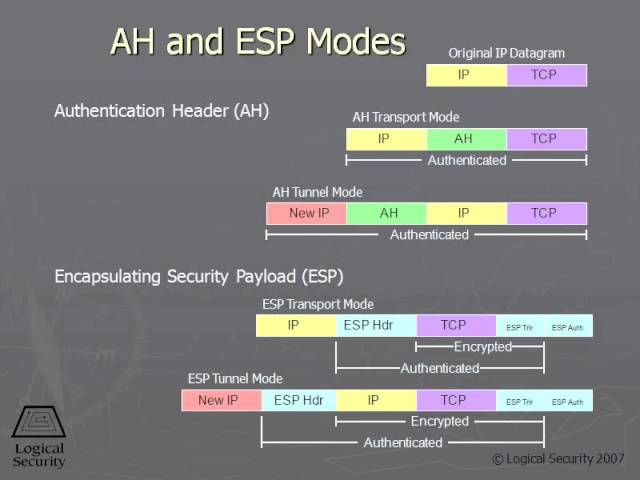
\includegraphics[width=0.86\linewidth]{assets/ipsec_ah_esp_modes.png}

\small\textit{Schéma AH a ESP režimů: AH hlavně autentizuje/integritně chrání, ESP přidává šifrování payloadu; transportní režim chrání původní paket mezi konci, tunelový režim zabalí celý původní IP paket do nového.}
\end{center}

TLS se nachází prakticky mezi transportní a aplikační vrstvou: běží nad TCP a poskytuje bezpečný kanál aplikačním protokolům. Proto vzniká HTTP na HTTPS, FTP na FTPS, případně zabezpečené varianty poštovních protokolů. TLS chrání komunikaci mezi dvěma koncovými body TLS spojení, ověřuje typicky server pomocí certifikátu a po handshake šifruje symetrickým klíčem.

Na aplikační vrstvě existují mechanismy jako PGP nebo S/MIME pro e-mail, aplikační podpisy, tokeny, vlastní autentizační protokoly a aplikační logika. Na linkové vrstvě záleží na technologii: Wi-Fi používá například WPA2/WPA3, podnikové linky mohou mít vlastní linkové zabezpečení, ale není to univerzální ochrana celé internetové cesty.

\itpr{\textbf{Mini box: jak funguje WPA2/WPA3 na Wi-Fi.} WPA chrání bezdrátový úsek mezi klientem a access pointem: nejdřív ověří, že klient zná správné tajemství nebo má správnou identitu, a potom šifruje rámce přenášené vzduchem. U domácího \textbf{WPA2-Personal} mají router i klient stejné heslo/PSK; heslo se neposílá vzduchem, ale použije se při \textbf{4-way handshake}, kde si strany přes nonce odvodí dočasné šifrovací klíče. Data se pak šifrují hlavně pomocí \textbf{AES-CCMP} a kontroluje se integrita, aby útočník nemohl rámce nepozorovaně měnit nebo přehrávat. Slabina WPA2-PSK je, že útočník může zachytit handshake a offline zkoušet hesla ze slovníku. \textbf{WPA3-Personal} nahrazuje PSK handshake metodou \textbf{SAE} (Dragonfly), která je odolnější proti offline hádání hesla a dává každému připojení vlastní klíč s lepší dopřednou bezpečností. Pro firmy je důležitý režim Enterprise, kde se místo sdíleného hesla používá typicky \textbf{802.1X/EAP} a autentizační server.}

VPN znamená virtuální privátní síť. V principu tuneluje provoz přes nedůvěryhodnou síť tak, že mezi klientem a VPN serverem nebo mezi dvěma gatewayemi vznikne chráněný tunel. VPN může chránit důvěrnost a integritu provozu na úseku do VPN brány, umožňuje autentizaci uživatele nebo zařízení a může způsobit, že se klient logicky chová jako součást vzdálené sítě. Neznamená ale automaticky anonymitu ani bezpečnost cílového serveru.

Pokud VPN končí ve firmě, poskytovatel cílové služby stále vidí provoz od VPN brány a aplikace musí být bezpečné samy o sobě.

Firewally filtrují provoz podle pravidel. Paketový filtr pracuje podle IP adres, portů a protokolů na L3/L4. Stateful \textbf{firewall} sleduje stav spojení, takže umí povolit odpovědi k již navázanému spojení. Aplikační firewall nebo NGFW umí kontrolovat obsah aplikačních protokolů, například HTTP, a \textbf{WAF} je specializovaný firewall pro webové aplikace proti útokům jako \textbf{SQL} injection, XSS nebo CSRF.

Proxy funguje jako prostředník: forward \textbf{proxy} řídí odchozí provoz klientů, reverse proxy chrání a zprostředkuje přístup k serverům, často s load balancingem a TLS terminací. \textbf{IDS} útoky detekuje a hlásí, \textbf{IPS} je navíc aktivně blokuje.

Na lokální síti se kromě firewallů uplatňují i ochrany přímo na druhé vrstvě, na switchích. \textbf{DHCP snooping} rozlišuje důvěryhodné a nedůvěryhodné porty a zahazuje DHCP odpovědi z nedůvěryhodných portů, čímž brání podvrženému (rogue) DHCP serveru a omezuje i \textbf{DHCP starvation}, tedy vyčerpání adresního poolu útočníkem. \textbf{Dynamic ARP Inspection} (DAI) kontroluje \textbf{ARP} zprávy proti tabulce z DHCP snoopingu a podvržené zahazuje, čímž brání ARP spoofingu.

Port security omezuje, kolik a jakých \textbf{MAC} adres smí být na portu, a port při porušení zablokuje. Client isolation zabrání tomu, aby spolu klienti na stejné síti, typicky Wi-Fi, navzájem komunikovali. \textbf{VLAN} \textbf{segmentace} odděluje provoz do logických sítí a \textbf{802.1X} vyžaduje autentizaci zařízení nebo uživatele dřív, než se port vůbec zpřístupní.

Dohromady tyto mechanismy řeší útoky, které firewall na hranici sítě nevidí, protože se odehrávají uvnitř jednoho L2 segmentu.

\itbox{\textbf{Vrstvové shrnutí:} Linková vrstva chrání konkrétní linku, IPsec chrání IP komunikaci, TLS chrání kanál pro aplikaci, PGP/S/MIME chrání přímo obsah zprávy. Čím výše zabezpečení leží, tím více rozumí konkrétní aplikaci; čím níže leží, tím transparentnější může být pro aplikace.}

\subsection*{9. Jak bych to celé řekl u státnic}

Síťové aplikace běží na aplikační vrstvě a používají aplikační protokoly, které definují formát, význam a pořadí zpráv. Mezi základní služby patří elektronická pošta, přenos souborů, web a DNS. U pošty se pro odesílání a předávání používá SMTP, zatímco pro vyzvedávání a synchronizaci schránky POP3 nebo IMAP.

U přenosu souborů je klasické FTP nezabezpečené a používá řídicí a datové spojení; FTPS je FTP přes TLS, zatímco SFTP je přenos souborů přes SSH. Web běží nad HTTP, zabezpečená varianta HTTPS používá TLS, které autentizuje server a šifruje komunikaci. DNS je hierarchická distribuovaná služba pro překlad jmen na IP adresy, kde se uplatňuje rekurzivní resolver, root, TLD a autoritativní servery.

Kvalita služby řeší, jaké vlastnosti od přenosu očekáváme: kapacitu, latenci, jitter a ztrátovost. Je důležitá hlavně pro multimédia, VoIP, videokonference a hry, protože ty jsou citlivé na zpoždění a kolísání. Mechanismy QoS zahrnují plánování front, priority, Weighted Fair Queuing, tvarování toků přes Leaky Bucket a Token Bucket a prevenci zahlcení pomocí RED/WRED.

Zabezpečení síťové komunikace řeší důvěrnost, integritu, autentizaci a nepopíratelnost. Symetrická kryptografie je rychlá, ale vyžaduje sdílený klíč; asymetrická kryptografie je pomalejší, ale umožňuje výměnu klíčů a digitální podpisy. V praxi se používá hybridní přístup. Na síťové vrstvě je typický IPsec, mezi transportní a aplikační vrstvou TLS, na aplikační vrstvě například PGP nebo S/MIME.

VPN vytváří chráněný tunel a používá autentizaci a šifrování k ochraně provozu přes nedůvěryhodnou síť.

\subsection*{10. Rychlá kontrola pojmů}

\begin{longtable}{p{0.475\linewidth}p{0.475\linewidth}}
\toprule
\textbf{Oblast} & \textbf{Co říct stručně} \\
\midrule\endhead
SMTP / POP3 / IMAP & SMTP odesílá a předává poštu; POP3 stahuje; IMAP synchronizuje schránku na serveru. \\
\addlinespace
FTP / FTPS / SFTP & FTP je nezabezpečené; FTPS = FTP přes TLS; SFTP = přenos souborů přes SSH; SCP = jednoduché kopírování přes SSH. \\
\addlinespace
DNS & Hierarchie: root, TLD, autoritativní server; rekurzivní resolver dotaz vyřeší a cacheuje. \\
\addlinespace
QoS & Metriky: bandwidth, latence, jitter, ztrátovost; metody: scheduling, token/leaky bucket, RED/WRED. \\
\addlinespace
TLS / IPsec / PGP & TLS chrání kanál aplikace, IPsec IP pakety, PGP/S/MIME obsah e-mailu. \\
\addlinespace
VPN & Tuneluje provoz přes nedůvěryhodnou síť; chrání úsek do VPN brány a autentizuje strany. \\
\addlinespace
\bottomrule
\end{longtable}

\newpage


\otazka{5. Principy programování}{Strukturované programování v imperativním jazyce. Paměťový model programu; správa paměti, dynamická alokace, práce s uživatelskými datovými strukturami. Nízkoúrovňová práce s pamětí, ukazatel, pole a ukazatelová aritmetika. Způsoby ladění programu (debugging). Bezpečné programování a vývoj SW.}{PB071, PV080}

\subsection*{5. Principy programování -- stručněji}
Otázka je hlavně o tom, jak program řízeně pracuje s výpočtem a pamětí. U nízkoúrovňového jazyka, typicky C, je důležité umět vysvětlit nejen algoritmus, ale i kde data leží a kdo odpovídá za jejich životnost.

\textbf{1. Strukturované imperativní programování}
\begin{itemize}
  \item Imperativní program říká počítači posloupnost kroků, které mění stav programu. Základ jsou proměnné, přiřazení, podmínky, cykly a funkce.
  \item Strukturované programování se snaží stavět program z čitelných bloků bez chaotických skoků. Cílem je, aby šel tok řízení sledovat a testovat.
\end{itemize}

\textbf{2. Paměťový model programu}
\begin{itemize}
  \item Běžně rozlišujeme kód, globální/statická data, haldu a zásobník. Zásobník drží lokální proměnné a návratové adresy, halda slouží pro dynamicky alokovaná data.
  \item Dynamická alokace znamená, že program za běhu žádá paměť, například přes \texttt{malloc}, a musí ji později uvolnit přes \texttt{free}. Chyby vedou k leakům, use-after-free nebo double free.
\end{itemize}

\textbf{3. Ukazatele, pole a struktury}
\begin{itemize}
  \item Ukazatel je proměnná obsahující adresu. Dereference znamená přístup k hodnotě na dané adrese.
  \item Pole v C úzce souvisí s ukazateli: jméno pole se často chová jako adresa prvního prvku. Ukazatelová aritmetika posouvá adresu po velikostech typu, ne po bajtech bez kontextu.
  \item Uživatelské datové struktury, například spojový seznam, strom nebo hash tabulka, stojí na kombinaci struktur, ukazatelů a dynamické alokace.
\end{itemize}

\textbf{4. Debugging}
\begin{itemize}
  \item Debugging je systematické hledání příčiny chyby. Používá se reprodukce, breakpointy, krokování, kontrola proměnných, logy, sanitizery a minimální testovací případ.
  \item Důležité je rozlišit symptom a příčinu: program může spadnout na jednom místě, ale paměť mohla být poškozena dávno předtím.
\end{itemize}

\textbf{5. Bezpečné programování}
\begin{itemize}
  \item Nejčastější nízkoúrovňová rizika jsou buffer overflow, use-after-free, integer overflow, formátovací řetězce, neinicializovaná paměť a chybějící kontrola návratových hodnot.
  \item Bezpečný vývoj znamená validovat vstupy, kontrolovat hranice, používat bezpečnější funkce, dělat code review, testy, statickou analýzu a kompilátorové ochrany.
\end{itemize}

\itbox{\textbf{Rozsah:} strukturované programování v imperativním jazyce, paměťový model programu, správa paměti, dynamická alokace, uživatelské datové struktury, nízkoúrovňová práce s pamětí, ukazatele, pole, ukazatelová aritmetika, debugging a bezpečné programování.}

\subsection*{Úvod: o čem u otázky mluvit}

Tahle otázka je hlavně o tom, že v nízkoúrovňovém programování už nevidím program jen jako sadu abstraktních příkazů, ale také jako konkrétní práci s pamětí. V jazyce C proměnná, pole, struktura, \textbf{ukazatel} i řetězec někde fyzicky leží v adresním prostoru procesu.

Programátor může s adresami přímo pracovat, a tím získává výkon a kontrolu, ale současně odpovědnost: C za něj běžně nehlídá meze pole, životnost objektů ani správné uvolnění dynamicky alokované paměti.

Začal bych strukturovaným a imperativním programováním, protože to je \textbf{rámec} celé otázky. Imperativní jazyk popisuje, jak se má výpočet provést krok za krokem: příkazy mění stav programu, tedy hodnoty proměnných a obsah paměti. Strukturované programování se snaží, aby program nebyl chaotický skok mezi instrukcemi, ale aby byl složený ze sekvence, větvení, cyklů a podprogramů.

Díky tomu jde problém rozdělit na menší funkce, každá funkce má jasnou odpovědnost, vstupy, výstupy a lokální proměnné.

U C je důležité dodat, že předávání parametrů je typicky hodnotou. Když funkci předám int, dostane kopii. Pokud chci, aby funkce změnila proměnnou volajícího, předám adresu, tedy ukazatel. To vypadá jako předávání referencí, ale v C se pořád předává hodnota - jen tou hodnotou je adresa. Tím se přirozeně dostávám k paměťovému modelu.

U strukturovaného programování je dobré zmínit také modularitu a čitelnost. Funkce by měla mít rozumně omezený účel, jasné parametry a dobře definovaný výsledek. V C se často rozlišuje vstupní parametr, který funkce jen čte, výstupní parametr, přes který funkce něco vrací pomocí ukazatele, a vstupně-výstupní parametr, který funkce čte i mění.

To je praktické například u funkcí, které mají vrátit více hodnot nebo měnit existující datovou strukturu.

\subsection*{Paměťový model procesu}

Když spustím program, operační systém mu vytvoří \textbf{proces} a proces dostane vlastní virtuální adresní prostor. Program tedy pracuje s virtuálními adresami. Překlad na fyzickou paměť řeší hardware, hlavně \textbf{MMU}, a operační systém pomocí stránkových tabulek. V rámci procesu se paměť tradičně dělí na několik částí: text neboli code \textbf{segment}, read-only data, data segment, BSS, \textbf{heap} a stack.

U zkoušky je dobré umět tento obrázek nakreslit a ukázat, kde bude lokální proměnná, globální proměnná a blok vrácený z mallocu.

\newpage
\begin{codebox}
\small
\begin{verbatim}
vyšší adresy
+----------------------------------+
| argumenty programu, prostředí    |
+----------------------------------+
| stack - lokální proměnné, rámce  |  roste typicky dolů
+----------------------------------+
| mapované oblasti, knihovny, mmap |
+----------------------------------+
| heap - bloky z malloc/calloc     |  roste typicky nahoru
+----------------------------------+
| BSS - neinicializované globální  |
+----------------------------------+
| data - inicializované globální   |
+----------------------------------+
| rodata - konstanty, literály     |
+----------------------------------+
| text/code - instrukce programu   |
+----------------------------------+
nižší adresy
\end{verbatim}
\end{codebox}

Text segment obsahuje strojové instrukce programu. Tam leží kód funkcí, například main nebo vlastní funkce. Typicky je tato oblast jen pro čtení a spouštění, aby program nemohl omylem nebo útokem přepisovat svůj vlastní kód.

Read-only data obsahují konstanty a často string literály, například text "ahoj". Data segment obsahuje inicializované globální a statické proměnné, například globální int nastavený na 10. BSS obsahuje globální a statické proměnné bez explicitní inicializace nebo inicializované nulou; při startu programu jsou vynulovány.

\itpr{\textbf{Mini pomůcka: .data vs. .bss.} \textbf{.data} obsahuje globální/statické proměnné s konkrétní počáteční hodnotou, takže tato hodnota musí být uložená i v programu na disku. \textbf{.bss} obsahuje proměnné nulové nebo bez explicitní inicializace; v souboru je hlavně informace o velikosti tohoto bloku a loader při spuštění vyhradí RAM a celý blok vynuluje. Tím se šetří hlavně místo v souboru na disku, ne RAM za běhu. Jakmile program běží, .data i .bss jsou normální zapisovatelná paměť a proměnná z .bss se po změně chová úplně stejně jako jiná globální proměnná.}

Stack neboli zásobník slouží hlavně pro volání funkcí. Při volání funkce vznikne stack frame, kde jsou lokální automatické proměnné, parametry, návratová adresa a často uložený stav předchozího rámce. Po návratu z funkce se její rámec zruší, a tím zaniknou její lokální proměnné. Heap neboli halda je oblast pro dynamickou alokaci. Pokud zavolám \textbf{malloc}, dostanu adresu bloku na heapu.

Tento blok nezanikne návratem z funkce, ale až tehdy, když ho explicitně uvolním pomocí free.

Správu paměti jde proto rozdělit na několik režimů. Statická paměť patří globálním a statickým objektům a existuje po celou dobu běhu programu. Automatická paměť patří lokálním proměnným na stacku a spravuje se automaticky podle běhu funkcí. Dynamická paměť je na heapu a její životnost řídí programátor. Právě dynamická paměť je nejčastějším zdrojem chyb, protože jazyk C za programátora nevykonává garbage collection.

\begin{longtable}{p{0.475\linewidth}p{0.475\linewidth}}
\toprule
\textbf{Příklad v C} & \textbf{Kam patří} \\
\midrule\endhead
int g = 10; & inicializovaná globální proměnná - data segment \\
\addlinespace
int g2; & neinicializovaná globální proměnná - BSS \\
\addlinespace
static int x = 5; & statická proměnná - data segment nebo BSS podle inicializace \\
\addlinespace
int local; & lokální automatická proměnná - stack \\
\addlinespace
int *p = malloc(sizeof *p); & p je lokální proměnná na stacku, ale blok, na který ukazuje, je na heapu \\
\addlinespace
char *s = "ahoj"; & s je ukazatel, samotný literál je typicky v read-only datech \\
\addlinespace
\bottomrule
\end{longtable}

Typická zkoušková věta: rozdíl je mezi proměnnou ukazatele a objektem, na který ukazuje. Lokální proměnná int *p může ležet na stacku, ale hodnota v ní je adresa bloku na heapu. To je přesně důvod, proč se často ptají, kde leží p a kde leží *p.

\subsection*{Stack vs. heap}

Stack je automaticky spravovaný. Když vstoupím do funkce, vytvoří se rámec; když se funkce vrátí, rámec zmizí. Proto je stack rychlý: alokace je v principu posun stack pointeru. Zároveň je ale omezený velikostí. Přesná velikost závisí na systému, nastavení a vlákně, typicky jde spíše o jednotky až desítky MB, ne o libovolně velkou paměť. Proto není dobré dávat na stack obrovská pole a hluboká rekurze může skončit stack \textbf{overflow}.

Heap je ručně spravovaný. Programátor explicitně řekne malloc nebo \textbf{calloc} a později musí říct free. Objekt na heapu může přežít návrat z funkce, což je užitečné například pro dynamické pole, spojový seznam nebo strom. Nevýhoda je, že programátor musí přesně vědět, kdo paměť vlastní a kdo ji uvolňuje. Pokud ji neuvolní, vzniká \textbf{memory leak}. Pokud ji uvolní dvakrát, vzniká \textbf{double free}.

Pokud ji po uvolnění ještě používá, vzniká \textbf{use-after-free}.

Vztah ke context switchi je takový, že každé \textbf{vlákno} má vlastní stack. Při přepnutí kontextu se uloží stav procesoru, zejména registry, program counter a stack pointer, aby se vlákno mohlo později vrátit přesně tam, kde skončilo. Heap je oproti tomu typicky sdílený všemi vlákny jednoho procesu. Proto když více vláken pracuje s daty na heapu, je potřeba synchronizace.

Při přepnutí mezi procesy se navíc může měnit celý virtuální adresní prostor, tedy i stránkové tabulky.

\subsection*{Dynamická alokace: malloc, calloc, realloc, free}

Dynamická alokace v C je založena na knihovních funkcích ze stdlib.h. Nejdůležitější jsou malloc, calloc, \textbf{realloc} a free. Funkce malloc má prototyp void *malloc(size\_t size). Vrací obecný ukazatel void * na blok o zadaném počtu bajtů. Pokud se alokace nepovede, vrátí NULL. Paměť z mallocu není inicializovaná, takže čtení jejího obsahu před zápisem je chyba.

\begin{codebox}
\small
\begin{verbatim}
#include <stdlib.h>
int *arr = malloc(n * sizeof *arr);
if (arr == NULL) {
    /* alokace selhala */
}
\end{verbatim}
\end{codebox}

Výraz sizeof je operátor, ne funkce. Vrací velikost typu nebo objektu v bajtech a výsledek má typ size\_t. Praktické je psát malloc(n * sizeof *arr), protože kdyby se změnil typ ukazatele arr, výraz zůstane správný. Pozor na to, že sizeof pole dává velikost celého pole, ale sizeof ukazatele dává jen velikost adresy. Když pole předám do funkce, rozpadne se na ukazatel na první prvek, takže funkce automaticky nezná jeho délku.

Funkce calloc alokuje paměť pro určitý počet prvků a vynuluje ji. Volání calloc(n, sizeof *arr) je tedy vhodné, když chci pole inicializované nulami. Funkce free uvolňuje blok, který byl získán z mallocu, callocu nebo reallocu. Do free se nesmí poslat adresa lokální proměnné ani ukazatel doprostřed bloku. free(NULL) je bezpečné a nic neudělá. Po free se obsah paměti nemaže spolehlivě a ukazatel se sám nenastaví na NULL.

Realloc mění velikost existujícího bloku. Může blok zvětšit na místě, zmenšit, nebo přesunout jinam a obsah překopírovat. Bezpečný vzor je použít dočasný ukazatel. Kdyby realloc selhal a já rovnou přepsal původní ukazatel, ztratil bych adresu starého bloku a vytvořil memory leak.

\begin{codebox}
\small
\begin{verbatim}
int *tmp = realloc(arr, new_n * sizeof *arr);
if (tmp == NULL) {
    /* arr je stale platny, muzeme ho uvolnit nebo dal pouzit */
} else {
    arr = tmp;
}
\end{verbatim}
\end{codebox}

\itbox{\textbf{Propojení s virtuální pamětí:} malloc je knihovní funkce v uživatelském prostoru. Pro malé alokace často používá oblast, kterou už má alokátor k dispozici. Když potřebuje více paměti, požádá operační systém například přes brk/sbrk nebo mmap. Vrácená adresa je virtuální adresa procesu. Fyzické stránky, stránkování a page fault řeší operační systém a MMU.}

\subsection*{Typické chyby při práci s pamětí}

Memory leak znamená, že program alokoval paměť a už ji neuvolní. Nejčastější varianta je, že lokální ukazatel na blok zanikne při návratu z funkce, ale blok na heapu zůstane alokovaný. U krátkého programu to nemusí být vidět, protože po skončení procesu operační systém paměť uklidí. U serveru nebo dlouho běžící aplikace je to vážná chyba.

\begin{codebox}
\small
\begin{verbatim}
void f(void) {
    int *p = malloc(sizeof *p);
    *p = 10;
} /* p zmizi, blok na heapu zustal: memory leak */
\end{verbatim}
\end{codebox}

Double free je uvolnění stejného bloku dvakrát. Může poškodit interní metadata alokátoru a v bezpečnostním kontextu může být zneužitelné. Nastavení ukazatele na NULL po free pomáhá jen částečně, protože mohou existovat aliasy, tedy jiné ukazatele na stejný blok. Use-after-free znamená, že po free s pamětí dál pracuji.

To je nedefinované chování: program může vypadat, že funguje, může spadnout, nebo může pracovat s pamětí, kterou už mezitím dostala jiná část programu.

Přístup mimo alokovanou paměť je další klasická chyba. C nekontroluje meze pole. Když mám int arr[10], platné indexy jsou 0 až 9. Zápis arr[10] je už za konec pole. U char bufferu to vede k \textbf{buffer overflow}, což je typická chyba, na kterou se u této otázky může komise zeptat. U stringů je navíc nutné počítat s ukončovacím nulovým znakem, takže pro text délky n potřebuji n + 1 znaků.

K typickým chybám patří i několik dalších, které je dobré umět pojmenovat. Integer overflow při výpočtu velikosti pro malloc nastane, když se velikost spočítá násobením, které přeteče rozsah typu; malloc pak alokuje menší blok, než program očekává, a následný zápis přeteče. S tím souvisí chyby signed/unsigned, kdy se záporné číslo přetypuje na velké kladné, například délka -1 uložená do size\_t se stane obrovským číslem.

Null pointer dereference je přístup přes ukazatel, který je NULL, typicky po neúspěšném mallocu nebo u neinicializovaného ukazatele. Dangling pointer je ukazatel na paměť, která už neexistuje (uvolněný blok nebo lokální proměnná po návratu z funkce); jeho použití je právě use-after-free. Off-by-one je chyba o jedničku, typicky zápis na \textbf{index} rovný délce pole nebo zapomenutí na nulový znak u řetězce.

Další skupina chyb souvisí s neopatrnou prací se vstupem a prostředím. Format string vulnerability vznikne, když se uživatelský vstup předá jako formátovací řetězec, například printf(vstup) místo printf("\%s", vstup); útočník pak může pomocí formátovacích značek číst nebo přepisovat paměť. Stack overflow je vyčerpání zásobníku, typicky příliš hlubokou nebo nekonečnou rekurzí.

Neověřené návratové hodnoty znamenají, že program ignoruje, zda funkce jako malloc, fopen nebo read uspěla, a pokračuje s neplatnou hodnotou. TOCTOU (time-of-check to time-of-use) je souběhová chyba, kdy se mezi kontrolou a použitím zdroje, například souboru, jeho stav změní a útočník toho zneužije.

Command injection vznikne, když se neověřený vstup vloží do příkazu pro shell, například přes system(); útočník tak může spustit vlastní příkazy.

\subsection*{Nedefinované chování (undefined behavior)}

Mnoho těchto chyb spadá pod takzvané nedefinované chování (\textbf{undefined behavior}, UB). To znamená, že \textbf{standard} jazyka pro danou situaci nepředepisuje vůbec nic: program může spadnout, vrátit nesmysl, nebo dokonce zdánlivě fungovat.

Ošemetné je, že chování se může lišit podle překladače a úrovně optimalizace, protože překladač předpokládá, že UB nikdy nenastane, a podle toho kód optimalizuje; stejný program tak může v ladicím a v optimalizovaném sestavení fungovat jinak. Typické příklady UB jsou přístup mimo pole, use-after-free, přetečení znaménkového celého čísla (signed overflow) a čtení neinicializované hodnoty.

Právě proto se na UB nelze spoléhat, ani když se kód zrovna "chová hezky".

\subsection*{Ukazatele: adresa, dereference, void pointer}

Ukazatel je proměnná, jejíž hodnota je adresa. Tedy ukazatel sám také někde leží v paměti, ale jeho obsahem je adresa jiného objektu. Operátor \& vrací adresu objektu. Operátor * při dereferenci zpřístupní hodnotu na adrese, na kterou ukazatel ukazuje.

\begin{codebox}
\small
\begin{verbatim}
int x = 10;
int *p = &x;
*p = 20;     /* meni x na 20 */
\end{verbatim}
\end{codebox}

\itpr{\textbf{Mini pomůcka k ukazatelům:} \texttt{p} je adresa, \texttt{*p} je objekt na této adrese. Když je \texttt{*p} vpravo od rovnítka, hodnotu čtu: \texttt{int y = *p;} vezme obsah krabičky. Když je \texttt{*p} vlevo od rovnítka, na tuto adresu zapisuji: \texttt{*p = 42;} přepíše původní hodnotu objektu. Naopak \texttt{p = 42;} by měnilo samotnou adresu uloženou v ukazateli, tedy kam ukazatel míří, ne hodnotu původní proměnné.}

Je potřeba přesně rozlišovat p, *p a \&p.; Samotné p je hodnota ukazatele, tedy adresa proměnné x. Výraz *p je hodnota objektu, na který p ukazuje. Výraz \&p; je adresa samotné proměnné p. Velikost pointeru není velikost objektu, na který ukazuje. Na běžném 64bitovém systému má ukazatel často 8 bajtů, ale int, double nebo struktura mohou mít jiné velikosti.

Void pointer, tedy void *, je obecný objektový ukazatel. Malloc ho vrací proto, aby mohl vrátit adresu paměti pro libovolný typ. V C se void * automaticky převede na konkrétní objektový pointer, například int *. Void pointer ale nejde standardně přímo dereferencovat, protože kompilátor neví, jaký typ objektu na adrese leží. A standardně s ním nelze dělat pointerovou aritmetiku, protože void nemá velikost.

Některé překladače to dovolí jako rozšíření, ale správně se má pro bajtovou aritmetiku použít char * nebo unsigned char *.

\subsection*{Pole, ukazatelová aritmetika a vícerozměrná pole}

Pole v C je souvislá oblast prvků stejného typu. Když zapíšu int arr[5], v paměti za sebou leží pět hodnot typu int. Název pole se ve většině výrazů převádí na ukazatel na první prvek, takže arr se často chová jako \&arr;[0]. Proto platí, že arr[i] je totéž jako *(arr + i). Pole a ukazatel ale nejsou totéž: sizeof arr dá velikost celého pole, zatímco sizeof p u ukazatele dá velikost adresy.

U pointerové aritmetiky je zásadní věta ke zkoušce: přičtení jedničky k ukazateli neznamená posun o jeden bajt, ale posun o jeden prvek daného typu. Pokud je p typu int *, pak p + 1 znamená posun o sizeof(int) bajtů. Pokud je p typu double *, posun je o sizeof(double) bajtů. U char * je posun o jeden bajt, protože sizeof(char) je 1.

\begin{codebox}
\small
\begin{verbatim}
int arr[4] = {10, 20, 30, 40};
int *p = arr;
*p        == 10
*(p + 1)  == 20     /* posun o jeden int, ne o jeden byte */
arr[2]    == *(arr + 2)
\end{verbatim}
\end{codebox}

Vícerozměrné pole, například int matrix[3][4], je v C uloženo po řádcích v souvislé paměti. Prvek matrix[row][col] odpovídá indexu row * počet\_sloupců + col v jednorozměrném pohledu. Při předávání dvourozměrného pole do funkce je potřeba znát počet sloupců, protože bez něj kompilátor neví, jak se má posunout na další řádek.

Dynamické pole se typicky alokuje přes malloc. U dynamické 2D matice jsou dvě běžné varianty: jeden souvislý blok, kde indexuji ručně přes row * cols + col, nebo pole ukazatelů na řádky. Souvislý blok je jednodušší pro \textbf{cache} a uvolňuje se jedním free. Pole ukazatelů umožní nepravidelné řádky, ale musí se uvolňovat každý řádek zvlášť a pak pole ukazatelů.

\subsection*{String v C}

String v C není speciální objekt s vlastní délkou. Je to pole znaků zakončené nulovým znakem '\textbackslash{}0'. Například řetězec "ahoj" má čtyři viditelné znaky, ale v paměti zabírá pět znaků: a, h, o, j a nulový znak. Funkce strlen vrátí 4, protože počítá znaky před nulovým znakem, zatímco sizeof u pole char s[] = "ahoj" vrátí 5.

\begin{codebox}
\small
\begin{verbatim}
char s[] = "ahoj";   /* modifikovatelne pole na stacku */
char *t = "ahoj";    /* t ukazuje na string literal, typicky read-only */
\end{verbatim}
\end{codebox}

Rozdíl mezi char s[] a char *t je zkouškově důležitý. Pole s obsahuje vlastní kopii znaků a můžu ho měnit. Ukazatel t ukazuje na string literál, který bývá v read-only paměti, a pokus o změnu t[0] je chyba. U stringů je typickým zdrojem bezpečnostních problémů buffer overflow, například při použití strcpy do příliš malého bufferu. Bezpečnější je pracovat s funkcemi, kde explicitně hlídám velikost bufferu, například fgets nebo snprintf.

\subsection*{Uživatelské datové struktury}

Do uživatelských datových struktur v C patří hlavně struct, union, enum a typedef. Struct spojuje více položek do jednoho typu. Například struktura uzlu spojového seznamu může obsahovat hodnotu a ukazatel na další uzel. Přístup k položce přes objekt se píše tečkou, přes ukazatel šipkou. Výraz p->next je zkratka za (*p).next. Velikost struktury nemusí být přesně součet velikostí položek, protože kompilátor může vložit zarovnávací mezery.

\begin{codebox}
\small
\begin{verbatim}
struct node {
    int value;
    struct node *next;
};
struct node *n = malloc(sizeof *n);
n->value = 10;
n->next = NULL;
\end{verbatim}
\end{codebox}

Union je podobný structu, ale položky sdílejí stejnou oblast paměti. V jednu chvíli tedy smysluplně drží jednu z hodnot. Enum slouží pro pojmenované konstanty a zlepšuje čitelnost kódu. Typedef zavádí alternativní jméno typu. U dynamických datových struktur, jako je spojový seznam, strom nebo dynamické pole, je podstatné vlastnictví paměti: kdo uzel vytvořil přes malloc, musí zajistit jeho uvolnění přes free.

U seznamu nestačí uvolnit jen hlavu, pokud tím ztratím odkazy na další uzly.

U struktur je vhodné zmínit i mělkou a hlubokou kopii. Při prostém přiřazení struktury se zkopírují hodnoty jejích položek. Pokud je ale položkou ukazatel na dynamicky alokovanou paměť, zkopíruje se jen adresa, ne data na heapu. Pak dvě struktury ukazují na stejný blok. Hluboká kopie znamená, že se alokuje nový blok a obsah se skutečně zkopíruje, aby každá struktura vlastnila vlastní paměť.

\subsection*{Debugging, testování a bezpečný vývoj}

Ladění programu znamená najít, proč se program nechová podle očekávání. V C je nutné brát vážně už varování překladače. Rozumný překlad pro vývoj je například gcc -Wall -Wextra -Wpedantic -g, kde -g přidá ladicí informace. Debugger, například gdb, umožňuje spustit program krok po kroku, nastavit breakpoint, vypsat hodnoty proměnných, dereferencovat ukazatele a zobrazit backtrace po pádu programu.

\textbf{Valgrind}, konkrétně nástroj Memcheck, pomáhá najít memory leak, čtení neinicializované hodnoty, neplatný zápis mimo blok, double free nebo use-after-free. Moderní alternativou jsou sanitizery, například AddressSanitizer přes volbu -fsanitize=address. Ty často velmi přesně ukážou, kde vznikl heap buffer overflow, stack buffer overflow nebo use-after-free.

Bezpečné programování v C znamená hlavně omezovat \textbf{riziko} nedefinovaného chování. Prakticky to znamená: kontrolovat návratové hodnoty mallocu a dalších funkcí, inicializovat proměnné, předávat do funkcí délku pole nebo velikost bufferu, nepoužívat paměť po free, neuvolňovat stejný blok dvakrát, hlídat přetečení indexů a velikostí, nepoužívat nebezpečné funkce typu gets a u textu vždy počítat s nulovým znakem.

U větších projektů k tomu patří unit testy, integrační testy, statická analýza a bezpečnostní testy v \textbf{CI/CD}.

U většího nebo bezpečnostně citlivého software se k tomu přidávají postupy nad rámec jednoho programu. Threat modeling už při návrhu hledá, kdo a jak by mohl systém napadnout. Code review znamená, že kód čte ještě další člověk. Statická analýza hledá chyby v kódu bez jeho spuštění, zatímco \textbf{fuzzing} program automaticky krmí náhodnými či záludnými vstupy a hledá pády.

Dependency scanning kontroluje použité knihovny na známé zranitelnosti a souvisí s pravidelnou aktualizací závislostí. Tyto kontroly se obvykle automaticky spouští v CI/CD. K bezpečnému provozu patří i správa tajemství (hesla a klíče nepatří do kódu, ale do správce tajemství), secure defaults (výchozí nastavení má být bezpečné už od začátku) a \textbf{least privilege} (program i jeho účet mají mít jen nutná oprávnění).

\subsection*{Závěrečná odpověď, kterou lze říct u zkoušky}

Kdybych měl otázku shrnout souvisle, řekl bych: V imperativním strukturovaném programování popisujeme výpočet krok za krokem pomocí sekvence, větvení, cyklů a funkcí. U nízkoúrovňového programování, typicky v C, je důležité chápat, že program pracuje s konkrétní pamětí.

Běžící proces má virtuální adresní prostor rozdělený na text segment s instrukcemi, read-only data s konstantami a string literály, data segment s inicializovanými globálními a statickými proměnnými, BSS s neinicializovanými nebo nulovými globálními a statickými proměnnými, heap pro dynamickou alokaci a stack pro volání funkcí, lokální proměnné a návratové adresy.

Stack je spravovaný automaticky, je rychlý, ale omezený velikostí a objekty na něm zanikají při návratu z funkce. Heap je spravovaný ručně přes malloc, calloc, realloc a free; objekty na něm žijí od alokace do uvolnění. Malloc vrací \textbf{void pointer} na neinicializovaný blok, calloc blok vynuluje, realloc mění velikost bloku a free ho uvolňuje. Při reallocu je bezpečné použít dočasný ukazatel.

Malloc pracuje nad virtuální pamětí procesu a alokátor si od operačního systému bere větší oblasti, které pak rozděluje na menší bloky.

Ukazatel je proměnná obsahující adresu. Operátor \& bere adresu, operátor * dereferencuje. Typ ukazatele určuje, jak se paměť interpretuje a jak funguje \textbf{ukazatelová aritmetika}. Přičtení jedničky k int pointeru není posun o jeden bajt, ale o velikost jednoho intu. Void pointer je obecný ukazatel, ale nelze ho standardně dereferencovat ani nad ním dělat aritmetiku bez převodu na konkrétní typ.

Pole je souvislá oblast prvků a ve výrazech se často převádí na ukazatel na první prvek; arr[i] je totéž jako *(arr + i), ale pole a ukazatel nejsou totéž, například podle sizeof.

String v C je pole znaků zakončené nulovým znakem. Proto musím vždy počítat s jedním znakem navíc. Typické chyby jsou memory leak, double free, use-after-free, přístup mimo pole, čtení neinicializované paměti a buffer overflow. Ladění se dělá pomocí varování překladače, gdb, Valgrindu, sanitizérů a testů.

Bezpečný vývoj znamená kontrolovat vstupy, velikosti bufferů, návratové hodnoty, životnost paměti a mít jasné vlastnictví dynamicky alokovaných objektů.

\itpr{\textbf{Na tabuli si pohlídat:} nakreslit paměť procesu; ukázat lokální proměnnou na stacku, globální v data/BSS a blok z mallocu na heapu; u pointerové aritmetiky říct, že +1 znamená posun o velikost typu; u stringu zmínit '\textbackslash{}0'; u chyb pojmenovat memory leak, double free, use-after-free a buffer overflow.}

\newpage


\otazka{6. Databáze}{Relační model, relační schéma, klíče relačních schémat, integritní omezení, relační algebra, spojování relací. Dotazovací jazyk SQL (příkaz select, spojování relací, agregační funkce). Zpracování dotazů. Indexování. Transakce. Vlastnosti transakčního zpracování.}{PB154 || PB168}

\subsection*{6. Databáze -- stručněji}
Databáze je řízené uložení dat tak, aby šla bezpečně sdílet, dotazovat, měnit a chránit proti nekonzistenci. Odpověď je dobré vést od relačního modelu přes SQL a indexy až k transakcím.

\textbf{1. Relační model}
\begin{itemize}
  \item Relační databáze ukládá data do relací, prakticky tabulek. Řádek je záznam, sloupec je atribut a relační schéma říká, jaké atributy tabulka má.
  \item Klíč jednoznačně identifikuje řádek. Primární klíč je zvolený hlavní identifikátor, cizí klíč odkazuje na řádek v jiné tabulce.
  \item Integritní omezení hlídají smysluplnost dat: doménová omezení, NOT NULL, UNIQUE, primární a cizí klíče.
\end{itemize}

\textbf{2. Relační algebra a SQL}
\begin{itemize}
  \item Relační algebra je formální základ dotazování: selekce vybírá řádky, projekce sloupce, spojení kombinuje tabulky podle vztahu.
  \item SQL je praktický dotazovací jazyk. Základní \texttt{SELECT} řeší \texttt{FROM}, \texttt{WHERE}, \texttt{JOIN}, \texttt{GROUP BY}, agregační funkce a \texttt{ORDER BY}.
  \item Join není jen "slepení tabulek"; vyjadřuje vztah mezi daty, typicky přes cizí klíč.
\end{itemize}

\textbf{3. Zpracování dotazů a indexy}
\begin{itemize}
  \item Databáze dotaz parsuje, optimalizuje a vytvoří plán provedení. Optimalizátor vybírá pořadí spojení, použití indexů a způsob čtení dat.
  \item Index zrychluje vyhledávání a řazení, ale zpomaluje zápisy a zabírá místo. Typický B+ strom umožní rychle hledat rozsahy i konkrétní hodnoty.
  \item Index není kouzlo na všechno: špatně zvolený index se nemusí použít, nízká selektivita moc nepomůže a příliš mnoho indexů zhorší update/insert.
\end{itemize}

\textbf{4. Transakce}
\begin{itemize}
  \item Transakce je skupina operací, která má proběhnout jako jeden logický celek. Vlastnosti ACID znamenají atomicitu, konzistenci, izolaci a trvanlivost.
  \item Atomicita: buď proběhne všechno, nebo nic. Izolace: souběžné transakce se nemají nebezpečně ovlivnit. Durability: po commitu data přežijí pád.
  \item Izolační úrovně řeší anomálie jako dirty read, non-repeatable read a phantom read. Vyšší izolace je bezpečnější, ale může snižovat výkon a zvyšovat blokování.
\end{itemize}

\subsection*{Relační model, SQL, zpracování dotazů, indexování a transakce}

Tato otázka spojuje dvě vrstvy databází: nejprve logický model dat, tedy \textbf{relační model}, schémata, klíče, \textbf{integritní omezení} a relační algebru, a potom praktickou práci v \textbf{SQL}, zpracování dotazů, indexování a transakční zpracování. U státnic je dobré nemluvit jen definice, ale pořád ukazovat, jak se z matematického pohledu dostaneme k tabulkám, dotazům a konkrétním problémům v praxi.

Komise se podle zápisů opakovaně ptaly na SQL syntaxi, klíče, normalizaci, \textbf{ACID} a indexy, takže odpověď by měla mít i malé příklady.

\subsection*{Relační model a relační schéma}

Relační model je databázový model, ve kterém jsou data reprezentována jako relace. Matematicky je relace množina n-tic, tedy množina uspořádaných řádků hodnot. Pokud má relace n atributů, mluví se o n-ární relaci. Formálně lze relaci chápat jako podmnožinu kartézského součinu domén D1 x D2 x ... x Dn. Prakticky v databázi tomu odpovídá tabulka: atributy jsou sloupce, n- tice jsou řádky a doména je množina povolených hodnot daného sloupce.

Například schéma Student(student\_id, jmeno, obor) říká, že relace Student má tři atributy. Jedna n-tice může být (1, Jan, Informatika). Z matematického pohledu je relace množina, takže neobsahuje duplicitní n-tice a nezáleží na pořadí řádků. Databázový pohled je implementační: tabulky mají datové typy, omezení, indexy a v SQL se mohou objevit duplicity, pokud jim nezabráníme klíčem nebo DISTINCT.

\begin{codebox}
\small
\begin{verbatim}
Student(student_id, jmeno, obor)
(1, Jan, Informatika)
(2, Eva, Kyberbezpečnost)
\end{verbatim}
\end{codebox}

Relační schéma je popis struktury relace: její název, seznam atributů a jejich domény. Samotná relace je až konkrétní aktuální množina řádků. Dobrá formulace ke zkoušce je: relační model je obecný princip práce s tabulkami, \textbf{relační schéma} je definice konkrétní tabulky a relace je aktuální obsah této tabulky.

\subsection*{Klíče a integritní omezení}

Klíče slouží k jednoznačné identifikaci řádků a ke spojování tabulek. Superklíč je libovolná množina atributů, která jednoznačně identifikuje řádek. Kandidátní klíč je minimální superklíč, tedy už z něj nejde odebrat atribut, aniž by se ztratila jednoznačnost. Primární klíč je jeden zvolený \textbf{kandidátní klíč}. Cizí klíč je atribut nebo množina atributů, které odkazují na klíč v jiné tabulce.

\begin{codebox}
\small
\begin{verbatim}
Student(student_id PRIMARY KEY, uco UNIQUE, jmeno)
Zapis(student_id FOREIGN KEY REFERENCES Student(student_id), predmet_id)
\end{verbatim}
\end{codebox}

Integritní omezení hlídají správnost dat. Entitní \textbf{integrita} říká, že \textbf{primární klíč} musí jednoznačně identifikovat řádek a nemá být NULL. Referenční integrita říká, že \textbf{cizí klíč} musí odkazovat na existující řádek v odkazované tabulce, případně být NULL, pokud to schéma dovoluje.

Doménová integrita omezuje hodnoty atributu podle typu a pravidel, například známka může být jen A až F. Prakticky se to v SQL vyjadřuje pomocí PRIMARY KEY, FOREIGN KEY, UNIQUE, NOT NULL nebo CHECK.

\begin{codebox}
\small
\begin{verbatim}
CREATE TABLE Hodnoceni (
  student_id INT NOT NULL,
  predmet_id INT NOT NULL,
  znamka CHAR(1) CHECK (znamka IN ('A','B','C','D','E','F')),
  PRIMARY KEY (student_id, predmet_id)
);
\end{verbatim}
\end{codebox}

Komise může chtít nakreslit tabulku a ukázat klíče. U vztahu 1:N je cizí klíč na straně N. U vztahu M:N se vytvoří spojovací tabulka, která má dva cizí klíče a často složený primární klíč. U vztahu 1:1 je cizí klíč navíc unikátní, nebo je přímo primárním klíčem druhé tabulky.

\subsection*{Relační algebra a spojování relací}

Relační algebra je formální dotazovací jazyk nad relacemi. Je procedurálnější než SQL: popisuje, jaké operace se nad relacemi provedou. Každá operace bere na vstupu relaci nebo relace a vrací opět relaci. Základní operace, které je potřeba umět namapovat na SQL, jsou selekce, projekce a spojení. Selekce vybírá řádky podle podmínky a značí se sigma. V SQL odpovídá hlavně klauzuli WHERE. Projekce vybírá sloupce a značí se pi.

V SQL odpovídá seznamu atributů za \textbf{SELECT}. Spojení relací propojuje řádky ze dvou tabulek podle podmínky, typicky podle primárního a cizího klíče.

\begin{codebox}
\small
\begin{verbatim}
Relační algebra:  pi jmeno ( sigma obor = 'Informatika' (Student) )
SQL: SELECT jmeno FROM Student WHERE obor = 'Informatika';
\end{verbatim}
\end{codebox}

Join je v databázích zásadní, protože normalizované schéma je rozdělené do více tabulek. Běžný INNER \textbf{JOIN} vrátí jen řádky, kde existuje odpovídající záznam na obou stranách. LEFT OUTER JOIN vrátí všechny řádky z levé tabulky a k nim odpovídající řádky zprava; pokud odpovídající řádek neexistuje, doplní se NULL. RIGHT JOIN je opačný a FULL OUTER JOIN zachová neodpovídající řádky z obou stran.

\begin{codebox}
\small
\begin{verbatim}
SELECT s.jmeno, p.nazev
FROM Student s
JOIN Zapis z ON s.student_id = z.student_id
JOIN Predmet p ON z.predmet_id = p.predmet_id;
\end{verbatim}
\end{codebox}

Přirozené spojení, NATURAL JOIN, automaticky spojuje podle všech stejně pojmenovaných atributů. Teoreticky odpovídá přirozenému spojení z relační algebry, ale prakticky je nebezpečné, protože může spojit i sloupce, které mají stejný název, ale jiný význam. U zkoušky je bezpečnější zdůraznit explicitní JOIN ON, kde přesně řeknu, podle čeho se tabulky spojují.

Kromě selekce, projekce a spojení má \textbf{relační algebra} ještě několik operací. Kartézský součin ($\times$) zkombinuje každý řádek jedné relace s každým řádkem druhé; spojení je vlastně \textbf{kartézský součin} následovaný selekcí.

Množinové operace pracují nad relacemi se stejnou strukturou, tedy stejnými atributy: sjednocení ($\cup$) vrátí řádky z obou relací, průnik ($\cap$) jen řádky společné oběma a rozdíl (-) řádky z první relace, které nejsou ve druhé. Přejmenování ($\rho$) změní jméno relace nebo atributů, což je užitečné například při spojení tabulky se sebou samou.

Spojení podle obecné podmínky (nejen rovnosti) se nazývá theta join; když je podmínkou rovnost stejnojmenných atributů a duplicitní sloupce se sloučí, jde o přirozené spojení (natural join). Okrajově existuje i relační dělení ($\div$), které odpovídá dotazům typu "najdi studenty zapsané do všech předmětů z dané množiny".

\subsection*{SQL: SELECT, DML, DDL a agregace}

SQL je praktický jazyk pro práci s relační databází. Základní SELECT má tvar SELECT - FROM - WHERE. SELECT říká, které sloupce chceme vrátit, FROM určuje zdrojové tabulky a WHERE filtruje řádky. Pro spojování se používá JOIN ON. SQL je deklarativní: uživatel popíše, co chce získat, ale konkrétní plán provedení vybírá optimalizátor databázového systému.

\begin{codebox}
\small
\begin{verbatim}
SELECT s.jmeno, COUNT(*) AS pocet_predmetu
FROM Student s
JOIN Zapis z ON s.student_id = z.student_id
WHERE s.obor = 'Informatika'
GROUP BY s.student_id, s.jmeno;
\end{verbatim}
\end{codebox}

DML, Data Manipulation Language, pracuje s konkrétními daty. Patří sem SELECT, INSERT, UPDATE a DELETE. DDL, Data Definition Language, definuje strukturu databáze. Patří sem CREATE TABLE, ALTER TABLE, DROP TABLE a CREATE INDEX. Komise se podle zápisů ptala i na CREATE TABLE, INSERT, UPDATE a ALTER TABLE, takže je dobré umět aspoň jednoduchý příklad.

\begin{codebox}
\small
\begin{verbatim}
CREATE TABLE Student (student_id INT PRIMARY KEY, jmeno VARCHAR(100));
INSERT INTO Student VALUES (1, 'Jan');
UPDATE Student SET jmeno = 'Jan Novak' WHERE student_id = 1;
ALTER TABLE Student ADD email VARCHAR(100);
\end{verbatim}
\end{codebox}

Agregační funkce počítají jednu souhrnnou hodnotu z více řádků. Typické jsou COUNT, SUM, AVG, MIN a MAX. Pokud chceme agregaci po skupinách, použijeme GROUP BY. Pokud chceme filtrovat jednotlivé řádky před seskupením, použijeme WHERE. Pokud chceme filtrovat až celé skupiny po agregaci, použijeme HAVING.

\begin{codebox}
\small
\begin{verbatim}
SELECT dept_name, AVG(salary) AS prumerny_plat
FROM Instructor
GROUP BY dept_name
HAVING AVG(salary) > 50000;
\end{verbatim}
\end{codebox}

Doplňkově se mohou objevit triggery a uložené procedury. Trigger je databázový objekt, který se automaticky spustí při události, například INSERT, UPDATE nebo DELETE. Hodí se pro audit, kontrolu pravidel nebo automatické doplnění odvozených dat, ale může skrývat vedlejší efekty. Uložená \textbf{procedura} je pojmenovaný blok kódu uložený v databázi, který lze opakovaně volat.

\subsection*{Normalizace a normální formy}

Normalizace je \textbf{proces} návrhu relačního schématu, při kterém se tabulky rozkládají tak, aby se snížila \textbf{redundance} a odstranily anomálie při vkládání, mazání a aktualizaci. Typický problém nenormalizované tabulky je opakování stejných údajů na mnoha řádcích. Když se například u každé objednávky opakuje jméno a adresa zákazníka, změna adresy vyžaduje aktualizovat mnoho řádků.

Pokud se některý řádek zapomene, vznikne inkonzistence. Normalizace se opírá o funkční závislosti. Zápis X -> Y znamená, že hodnota atributů X jednoznačně určuje hodnotu atributů Y. Například student\_id -> jmeno znamená, že pokud znám ID studenta, znám jeho jméno. Funkční závislosti nevznikají z názvů atributů, ale z významu dat a pravidel dané domény.

Předpokladem u \textbf{2NF}, \textbf{3NF} a \textbf{BCNF} je existence netriviální funkční závislosti X -> Y:

\begin{longtable}{p{0.237\linewidth}p{0.237\linewidth}p{0.237\linewidth}p{0.237\linewidth}}
\toprule
\textbf{Normální forma} & \textbf{Formální pravidlo pro X -> Y} & \textbf{Lidsky vysvětleno} & \textbf{Důraz na typy klíčů} \\
\midrule\endhead
1NF & (Neřeší se přes X -> Y) & Každá buňka obsahuje jen jednu nedělitelnou atomickou hodnotu. Žádná pole, seznamy ani opakující se skupiny. & Není relevantní. \\
\addlinespace
2NF & Pokud Y není součástí žádného klíče, X nesmí být jen ostrou podmnožinou klíče. & Obyčejný neklíčový údaj nesmí záviset pouze na kousku složeného klíče. & Levá strana nesmí být pouhá část kandidátního klíče. \\
\addlinespace
3NF & Platí alespoň jedno: X je superklíč, nebo Y je součástí kandidátního klíče. & Levá strana jednoznačně určuje celý řádek, nebo se aplikuje výjimka, protože vpravo je důležitá součást identifikátoru. & Vlevo superklíč, nebo jako výjimka vpravo atribut kandidátního klíče. \\
\addlinespace
BCNF & Musí vždy platit: X je superklíč. & Cokoliv, co v tabulce určuje něco jiného, musí umět určit úplně celý řádek. Bez výjimek. & Vlevo čistě jen superklíč; pravá strana se neřeší. \\
\addlinespace
\bottomrule
\end{longtable}

Jednoduchý příklad porušení \textbf{1NF} je Student(student\_id, jmeno, telefony), kde je v jedné buňce seznam telefonů. Správně se telefony přesunou do samostatné tabulky Telefon(student\_id, telefon). Porušení 2NF typicky vzniká u tabulky PolozkaObjednavky(objednavka\_id, produkt\_id, nazev\_produktu, cena, mnozstvi), kde klíč je (objednavka\_id, produkt\_id), ale název a cena produktu závisí jen na produkt\_id.

Porušení 3NF vzniká například u Student(student\_id, jmeno, obor\_id, nazev\_oboru), protože student\_id určuje obor\_id a obor\_id určuje nazev\_oboru. Název oboru proto patří do tabulky Obor.

Vztah mezi normálními formami je hierarchický: BCNF implikuje 3NF, 3NF implikuje 2NF a 2NF implikuje 1NF. Opačně to neplatí. 3NF je slabší než BCNF, protože připouští výjimku, když je pravá strana funkční závislosti součástí kandidátního klíče. BCNF je čistší: levá strana každé netriviální funkční závislosti musí být superklíč.

Normalizace typicky zlepšuje konzistenci dat, ale nemusí automaticky zvyšovat výkon, protože více tabulek znamená více spojování.

\subsection*{Zpracování dotazů}

Když uživatel napíše SQL dotaz, databázový systém ho nejdříve zparsuje a ověří, že syntaxe, tabulky a sloupce dávají smysl. Potom ho převede do interní reprezentace, často podobné relační algebře. Následuje optimalizace: databáze hledá vhodný plán provedení. Nakonec vykonávací engine plán provede.

Důležité je, že SQL neříká přesný postup provedení. Jeden dotaz lze provést více způsoby: full table scanem, \textbf{index} scanem, různým pořadím joinů nebo různým způsobem materializace mezivýsledků. Optimalizátor se snaží minimalizovat náklady, hlavně počet načtených bloků z disku, práci s pamětí a velikost mezivýsledků. Typické heuristiky jsou provádět selekce co nejdříve, projekce co nejdříve a nejrestriktivnější operace před drahými joiny.

\begin{codebox}
\small
\begin{verbatim}
SELECT z.jmeno, p.nazev
FROM Zakaznik z
JOIN Objednavka o ON z.id = o.zakaznik_id
JOIN Polozka po ON o.id = po.objednavka_id
JOIN Produkt p ON po.produkt_id = p.id
WHERE z.mesto = 'Brno' AND p.kategorie = 'Notebook';
\end{verbatim}
\end{codebox}

U tohoto dotazu je výhodné nejdříve vybrat zákazníky z Brna a produkty kategorie Notebook, a teprve potom spojovat. Pokud by databáze nejdřív spojila všechny zákazníky, objednávky, položky a produkty, vznikly by zbytečně velké mezivýsledky. Vyhodnocování může probíhat materializací, kdy se mezivýsledek uloží jako dočasná relace, nebo pipeliningem, kdy se řádky posílají dalším operátorům průběžně bez uložení celého mezivýsledku.

Konkrétní operace v plánu mají různé fyzické implementace a právě mezi nimi optimalizátor vybírá. Přístup k tabulce může být \textbf{full table scan}, kdy se přečtou všechny bloky tabulky (vhodné, když dotaz vrací velkou část řádků nebo není použitelný index), nebo \textbf{index scan}, kdy se nejdřív najdou odkazy v indexu a načtou se jen vybrané řádky (vhodné, když podmínka vybírá málo řádků).

Spojení dvou tabulek lze provést několika algoritmy. Nested-loop join pro každý řádek jedné tabulky projde druhou; je jednoduchý a dobrý pro malé tabulky. Index \textbf{nested-loop join} je jeho zrychlení, kdy se k vyhledání odpovídajících řádků druhé tabulky použije index, což se hodí, když je vnější tabulka malá a vnitřní má index na spojovacím sloupci.

Hash join si z menší tabulky postaví hašovací tabulku podle spojovacího klíče a druhou tabulkou jí prožene řádky; je výborný pro velké tabulky a spojení přes rovnost. Sort-merge join obě tabulky seřadí podle spojovacího klíče a pak je naráz prochází; vyplatí se, když jsou data už seřazená nebo když stejně potřebujeme seřazený výsledek.

Aby se optimalizátor mohl rozhodnout, je \textbf{cost-based}, tedy odhaduje náklady jednotlivých plánů. K tomu používá statistiky o datech (počty řádků, počty různých hodnot, rozložení hodnot), z nichž odhaduje selektivitu podmínky, tedy jakou část řádků podmínka propustí, a kardinalitu, tedy kolik řádků bude mít daný mezivýsledek. Z toho spočítá očekávaný počet přístupů na disk a vybere nejlevnější plán.

Když je potřeba seřadit velký výsledek, který se nevejde do paměti, použije se external sorting (vnější třídění), které řadí po částech na disku a pak je slévá. Špatné nebo zastaralé statistiky jsou častou příčinou toho, že optimalizátor zvolí pomalý plán.

U dřívějšího dotazu na zákazníky z Brna a notebooky lze stejnou logiku provést různými fyzickými plány. Jedna možnost: index scan vybere zákazníky z Brna a produkty kategorie Notebook a pak se postupně index nested-loop joiny napojí objednávky a položky přes indexy na cizích klíčích. Druhá možnost při velkých tabulkách: full table scany s následnými \textbf{hash} joiny přes rovnost klíčů.

Třetí možnost, pokud jsou data vhodně seřazená: \textbf{sort-merge join}. Všechny vrátí stejný výsledek, ale liší se náklady, a právě proto optimalizátor potřebuje statistiky.

\subsection*{Indexování, hašování a B+ stromy}

Index je pomocná datová struktura, která urychluje hledání dat podle vyhledávacího klíče. Místo toho, aby databáze procházela celou tabulku, najde hodnotu v indexu a podle odkazu načte odpovídající řádek nebo blok. Trade-off je zásadní: indexy zrychlují čtení, hledání, joiny a často ORDER BY, ale zabírají místo navíc a zpomalují INSERT, UPDATE a DELETE, protože se musí aktualizovat nejen tabulka, ale i indexy.

\begin{codebox}
\small
\begin{verbatim}
CREATE INDEX idx_zakaznik_email ON Zakaznik(email);
SELECT * FROM Zakaznik WHERE email = 'jan@example.com';
\end{verbatim}
\end{codebox}

Hustý index obsahuje položku pro každou hodnotu vyhledávacího klíče nebo přímo pro každý záznam. U neunikátních hodnot může jedna hodnota ukazovat na více řádků. Řídký index obsahuje položky jen pro některé hodnoty, typicky pro první hodnotu v bloku. Aby řídký index fungoval, musí být datový soubor fyzicky seřazený podle vyhledávacího klíče; jinak by index nevěděl, kde hledat další hodnoty.

Primární nebo shlukovací index je takový, jehož klíč určuje fyzické pořadí záznamů v souboru. Proto může být řídký. Sekundární index je index nad jiným atributem, než podle kterého jsou data fyzicky uložena. Proto bývá hustý, protože odpovídající řádky mohou být rozházené po celé tabulce. Například tabulka je uložená podle student\_id, ale vytvoříme sekundární index nad jmeno.

Hash index používá hashovací funkci, která hodnotu klíče mapuje do bucketu. Je vhodný pro přesné hledání podle rovnosti, například WHERE email = ... nebo WHERE id = ..., protože databáze spočítá hash a jde rovnou do bucketu. Nehodí se ale pro rozsahové dotazy a řazení, protože hash nezachovává pořadí hodnot. Proto se pro rozsahy používá spíše stromový index, typicky B+ strom.

\begin{codebox}
\small
\begin{verbatim}
Hash index: dobrý pro WHERE id = 123
B+ strom: dobrý pro WHERE datum BETWEEN ... AND ..., ORDER BY datum i WHERE id = 123
\end{verbatim}
\end{codebox}

B+ strom je vyvážená stromová struktura používaná pro databázové indexy. Vnitřní uzly slouží k navigaci a listy obsahují klíče s odkazy na záznamy; listy jsou navíc propojené, což pomáhá rozsahovým dotazům.

Na otázku, proč se pro databázové indexy nepoužívá MD5 nebo SHA1, je odpověď: kryptografický hash je dobrý pro otisk hodnoty, ale nezachovává pořadí, neřeší přirozeně rozsahy a jeho cílem není fyzická organizace databázových stránek ani efektivní průchod listy jako u B+ stromu.

U indexů je dobré znát ještě několik praktických pojmů. Shlukovací (clustered) index určuje fyzické pořadí řádků v tabulce, takže jich může být jen jeden; neshlukovací (non-clustered) index je oddělená struktura s odkazy na řádky a může jich být víc.

Složený (composite) index je index nad více sloupci najednou a velmi záleží na pořadí sloupců: index nad (prijmeni, jmeno) pomůže dotazu podle samotného příjmení nebo podle příjmení a jména, ale ne dotazu jen podle jména. Pokrývající (covering) index obsahuje přímo všechny sloupce, které dotaz potřebuje, takže databáze odpověď přečte z indexu a vůbec nemusí sáhnout do tabulky.

Jak už bylo řečeno, indexy nejsou zadarmo: každý další index zpomaluje INSERT, UPDATE i DELETE, protože se při změně dat musí aktualizovat i všechny indexy.

\subsection*{Transakce a vlastnosti transakčního zpracování}

Transakce je logická jednotka práce nad databází. Typický příklad je převod peněz mezi účty: částka se musí z jednoho účtu odečíst a na druhý přičíst. V SQL transakci typicky ohraničíme pomocí BEGIN TRANSACTION, COMMIT a případně ROLLBACK. Databázový systém potom zajišťuje vlastnosti ACID: \textbf{atomičnost}, konzistenci, izolaci a trvalost.

\begin{codebox}
\small
\begin{verbatim}
BEGIN TRANSACTION;
UPDATE Ucet SET zustatek = zustatek - 1000 WHERE id = 'A';
UPDATE Ucet SET zustatek = zustatek + 1000 WHERE id = 'B';
COMMIT;
\end{verbatim}
\end{codebox}

Atomičnost znamená, že \textbf{transakce} proběhne celá, nebo vůbec. Když se převod přeruší po odečtení z účtu A, musí se změna vrátit, protože by se peníze ztratily. Konzistence znamená, že transakce převádí databázi z jednoho konzistentního stavu do druhého a respektuje integritní omezení. Izolace znamená, že souběžné transakce nemají vidět nekonzistentní mezistavy jiných transakcí. Trvalost znamená, že po commitu změny přežijí i pád systému.

Formálním kritériem \textbf{izolace} je \textbf{serializovatelnost}. Souběžný plán je serializovatelný, pokud jeho výsledek odpovídá nějakému sériovému pořadí transakcí. Transakce se tedy mohou fyzicky prokládat, ale výsledek musí být stejný, jako kdyby běžely jedna po druhé. Konfliktní operace jsou operace různých transakcí nad stejnou položkou, kde alespoň jedna je zápis: read-write, write- read nebo write-write.

Konkrétní problémy souběhu je dobré umět pojmenovat. Dirty read nastane, když transakce čte nepotvrzená data jiné transakce, která se pak může rollbacknout. Lost update nastane, když dvě transakce přečtou stejnou hodnotu, obě ji upraví a jedna aktualizace přepíše druhou. Non-repeatable read nastane, když transakce přečte stejný řádek dvakrát a pokaždé dostane jinou hodnotu, protože jiná transakce mezi tím commitovala změnu.

Phantom read nastane, když opakovaný dotaz s podmínkou vrátí jinou množinu řádků, protože jiná transakce vložila nebo smazala řádky splňující podmínku.

Souběhové problémy se nejčastěji řeší zamykáním. Sdílený zámek (shared, S) slouží pro čtení a může ho na téže položce držet více transakcí zároveň. Výlučný zámek (exclusive, X) slouží pro zápis a smí ho držet jen jedna transakce; je nekompatibilní jak s dalším X, tak s S zámkem. Tato kompatibilita zámků zajišťuje, že se zápis nepotká se souběžným čtením ani jiným zápisem téže položky.

Aby zamykání zaručilo serializovatelnost, používá se dvoufázové zamykání (\textbf{two-phase locking}, 2PL). Každá transakce má rostoucí fázi (growing phase), ve které jen získává zámky, a klesající fázi (shrinking phase), ve které je už jen uvolňuje; jakmile jednou nějaký zámek uvolní, nesmí získat žádný nový.

Zamykání ale může vést k deadlocku mezi transakcemi: T1 drží zámek na A a čeká na B, zatímco T2 drží B a čeká na A. Databáze \textbf{deadlock} detekuje (typicky v grafu čekání) a jednu z transakcí zruší a rollbackne.

V praxi se míra izolace nastavuje pomocí izolačních úrovní, které dovolují kompromis mezi výkonem a přísností: READ UNCOMMITTED (dovolí i \textbf{dirty read}), READ COMMITTED (zakáže dirty read), REPEATABLE READ (zakáže i non-repeatable read) a SERIALIZABLE (nejpřísnější, brání i phantomům). Nižší úrovně jsou rychlejší, ale připouštějí více anomálií.

Mnoho moderních databází navíc používá \textbf{MVCC} (multiversion concurrency control): místo aby čtení a zápisy blokovaly jeden druhého, drží se více verzí řádku a každá transakce čte konzistentní snímek (\textbf{snapshot}) dat z určitého okamžiku. Čtenáři tak neblokují zapisovatele a naopak, což výrazně zlepšuje souběžnost.

Rollback znamená zrušení transakce a vrácení databáze do stavu před jejím začátkem. S tím souvisí obnovitelnost plánů: pokud T2 čte hodnotu zapsanou T1, měla by T1 commitnout dříve než T2. Jinak by T2 mohla potvrdit výsledek založený na datech, která se později rollbacknou. Kaskádový rollback nastává, když selhání jedné transakce vyvolá rollback dalších transakcí, které četly její nepotvrzená data.

Pro obnovu po selhání se používá logování. Databáze si do logu zapisuje, co transakce změnily, a při obnově provádí UNDO u nepotvrzených transakcí a REDO u potvrzených transakcí. Aby obnova nemusela procházet celý log od začátku, databáze pravidelně vytváří \textbf{checkpoint}, tedy bod, ke kterému jsou změny bezpečně zapsané; po pádu pak stačí log procházet zhruba od posledního checkpointu.

Důležitý princip je \textbf{write-ahead} logging: log o změně se musí zapsat dříve než samotná změněná databázová \textbf{stránka}. Alternativou jsou stínové databáze neboli shadow paging: původní stránky se nepřepisují, změny se dělají do kopií a při commitu se atomicky přepne \textbf{ukazatel} na novou verzi. Výhodou je jednoduchý rollback, nevýhodou režie, \textbf{fragmentace} a horší souběžnost.

\subsection*{Krátká závěrečná osnova odpovědi}

U zkoušky bych odpověď uzavřel takto: Databáze v relačním modelu ukládá data jako relace, tedy tabulky, jejichž strukturu popisuje relační schéma. Řádky jsou n-tice, sloupce atributy a hodnoty atributů patří do domén. Správnost a jednoznačnost zajišťují klíče a integritní omezení. Nad relacemi formálně pracuje relační algebra, hlavně selekce, projekce a spojení, což se v SQL projeví jako SELECT, WHERE a JOIN.

SQL dále umožňuje agregace pomocí COUNT, SUM, AVG, MIN a MAX, definici schématu pomocí DDL a změny dat pomocí DML. Dotazy se v DBMS parsují, optimalizují a provádějí podle vybraného plánu. Indexy urychlují hledání, ale stojí prostor a zpomalují zápisy; hash index je dobrý na rovnost, B+ strom i na rozsahy.

Transakce zajišťují ACID, izolace se formálně váže na serializovatelnost, při chybě se použije rollback a obnova se řeší logováním nebo stínovými databázemi.

\begin{codebox}
\small
\begin{verbatim}
Materiál vytvořen jako souvislé opakování k otázce 6 podle dodaného PDF a stop z databáze komisí.
\end{verbatim}
\end{codebox}

\newpage


\otazka{7. Softwarové a informační systémy}{Vývoj a provoz softwarových systémů. Použití UML při vývoji software. Aplikované informační systémy. Architektury rozsáhlých informačních systémů. Metody vedení rozsáhlých projektů. Řízení provozu IS.}{PB007, PV028}

\itbox{\textbf{Cíl odpovědi:} ukázat, že informační systém není jen program, ale celek lidí, dat, procesů, hardwaru a softwaru. U státnic je dobré postupovat od životního cyklu a požadavků přes modelování a testování až k architektuře, projektovému řízení a provozu. Praktická pointa je, že systém musí být nejen vyvinut, ale také provozován, udržován, měněn, monitorován a smluvně zajištěn.}

\begin{greenbox}
\textbf{Modelová odpověď v přesném pořadí otázky podle dodaných zdrojů}

\textbf{1. Softwarové a informační systémy.} Začal bych vymezením. \textbf{Software} je programové vybavení, tedy aplikace, služby, knihovny nebo komponenty, které vykonávají určitou činnost. \textbf{Informační systém} je širší socio-technický celek: lidé, hardware, software, data, procesy a pravidla, které zajišťují sběr, přenos, zpracování, uchování a prezentaci informací pro plánování, rozhodování a řízení. Operační systém nebo middleware samy o sobě ještě nejsou informační systém; jsou to podpůrné technologie. IS vzniká až tehdy, když nad daty pracují konkrétní uživatelé v rolích a systém podporuje reálný proces organizace.

\textbf{2. Vývoj a provoz softwarových systémů.} Vývoj bych popsal přes SDLC, tedy životní cyklus softwaru: \textbf{plánování a požadavky -- analýza -- návrh -- implementace -- testování -- nasazení -- provoz -- údržba a další vývoj}. Cílem SDLC je dodat software efektivně, v požadované kvalitě a tak, aby byl udržovatelný. Důležité je rozlišit \textbf{funkční požadavky}, tedy co systém dělá, a \textbf{nefunkční požadavky}, tedy v jaké kvalitě to dělá: dostupnost, výkon, bezpečnost, auditovatelnost, škálovatelnost nebo použitelnost. Provoz není dodatek až po projektu. Už při návrhu se musí myslet na monitoring, logy, zálohy, obnovu, správu verzí, podporu uživatelů, bezpečnostní aktualizace a změnové řízení. Pokud jde o bezpečný vývoj, SSDLC přidává bezpečnost do každé fáze: bezpečnostní požadavky, threat modeling, bezpečný návrh, statickou analýzu, bezpečnostní testy a provozní monitoring.

\textbf{3. Použití UML při vývoji software.} UML je standardizovaný grafický jazyk pro modelování systému. Jeho smysl není kreslit obrázky pro obrázky, ale vytvořit společný jazyk mezi zákazníkem, analytikem, vývojářem, testerem a provozem. \textbf{Use-case diagram} se hodí na začátku pro aktéry, hranice systému a požadavky. \textbf{Activity diagram} popisuje workflow procesu, například vyřízení žádosti nebo objednávky. \textbf{Class diagram} ukazuje strukturu domény nebo návrhu, tedy třídy, atributy a vztahy. \textbf{Sequence diagram} ukazuje komunikaci v čase, třeba volání mezi webem, API a databází. \textbf{Deployment diagram} ukazuje fyzické nebo virtuální nasazení: klient, web server, aplikační server, databáze, message broker nebo cloud. ER diagram a DFD nejsou UML v úzkém smyslu, ale ve zdrojích dávají smysl jako doplněk: ER pro databázový model, DFD pro toky dat a bezpečnostní/threat modeling.

\textbf{4. Aplikované informační systémy.} Aplikovaný IS je rozsáhlejší systém zasazený do konkrétní domény. Typicky jej používá více uživatelů v různých rolích, pracuje nad společnými daty v databázi, podporuje workflow a často běží jako klient-server nebo webový systém. V nemocnici AIS podporuje příjem pacienta, hospitalizaci, žádanky, laboratorní výsledky, medikaci, pojišťovny a role lékaře, sestry, laboratoře a administrativy. Ve veřejné správě AIS přijímá žádosti, vede spis, pracuje s číslem jednacím, registry a doručováním. V e-shopu se propojuje katalog, objednávka, sklad, platba, doprava, fakturace a reklamace. U environmentálních IS je dobré zmínit logiku monitoring -- data -- informace -- assessment -- reporting: stát sbírá data, kontroluje jejich kvalitu, převádí je na použitelné informace a reportuje je podle právních povinností, například vůči EU.

\textbf{5. Architektury rozsáhlých informačních systémů.} U architektur bych šel přes to, co zdroje výslovně chtějí slyšet: \textbf{třívrstvá architektura, MVC, SOA, mikroslužby, škálování a kontejnerizace}. Třívrstvá architektura dělí systém na prezentační vrstvu, aplikační vrstvu s business logikou a databázovou vrstvu. MVC je vzor uvnitř aplikace: Model drží data a pravidla, View zobrazuje a Controller zpracovává vstup. SOA chápe systém jako soubor spolupracujících služeb s rozhraními; mikroslužby jsou jemnější varianta s menšími samostatně nasazovanými službami. Rozsáhlý IS musí být škálovatelný, spolehlivý, bezpečný a efektivní. Škálování může být vertikální, tedy silnější server, nebo horizontální, tedy více instancí za load balancerem. Docker a Kubernetes patří k provoznímu nasazení: kontejnery balí aplikaci se závislostmi, Kubernetes je orchestruje, škáluje a restartuje.

\textbf{6. Metody vedení rozsáhlých projektů.} U velkých projektů bych zdůraznil, že bývají \textbf{iterativní a inkrementální}. Iterace je opakovaný vývojový cyklus, inkrement je konkrétní přírůstek funkcionality. Ze zdrojů je důležité říct \textbf{Unified Process/RUP}, případně kombinaci s PRINCE2 nebo IPMA. UP je iterativní a inkrementální, řízený riziky a případy užití, zaměřený na architekturu a podporovaný UML. Pro plánování se používá WBS pro rozpad práce, PERT pro odhad pracnosti a času, Ganttův diagram pro harmonogram, síťový diagram a kritická cesta pro zjištění úkolů, které nesmí sklouznout bez posunu celého projektu. U rozsáhlého projektu je nutné řídit rizika, komunikaci, eskalace, změny, rozpočet, milníky, akceptace, dodavatele a kvalifikaci týmu.

\textbf{7. Řízení provozu IS.} Provoz IS znamená zajistit, aby systém dlouhodobě poskytoval službu v dohodnuté kvalitě. Patří sem monitoring, helpdesk, incident management, problem management, change management, profylaxe, zálohování, obnova, dokumentace, správa kapacity, bezpečnost a komunikace s uživateli. \textbf{SLA} určuje servisní hodiny, kategorie incidentů, reakční dobu, dobu opravy, dostupnost, komunikační kanály, cenu a sankce. Kritický výpadek produkčního nemocničního systému se tedy řeší jinak než kosmetická chyba v interním reportu. Cena podpory může být částečně paušální a částečně položková podle rozsahu zásahů. Závěrečná věta: úspěšný IS se nepozná jen podle toho, že byl naprogramován, ale podle toho, že v provozu spolehlivě podporuje proces organizace, zvládá změny a má jasně nastavenou odpovědnost.
\end{greenbox}

\begin{greenbox}
\textbf{Doplňková praktická odpověď: aplikovaný informační systém, architektura, projekt a provoz}

Kdybych dostal otázku na softwarové a informační systémy a chtěl odpovědět co nejpraktičtěji, začal bych pojmem \textbf{aplikovaný informační systém}. AIS není jedna malá aplikace, ale \textbf{soubor aplikací, databází, uživatelů, rolí, workflow a integračních vazeb}, který umožňuje více lidem v organizaci pracovat nad společnými daty. Typicky jde o webový nebo klient-server systém: uživatel pracuje v prohlížeči nebo klientské aplikaci, aplikační server provádí business logiku a databázová vrstva drží sdílená data. Pointa je, že AIS podporuje reálný proces organizace, například léčbu pacienta, vyřízení žádosti, prodej zboží, skladové hospodářství nebo úřední řízení.

\textbf{Data a databáze.} Data jsou obvykle uložena v databázích, protože více uživatelů musí pracovat nad stejnými záznamy konzistentně a současně. Relační databáze, například PostgreSQL, Oracle nebo MySQL, ukládá data do tabulek a vztahů: pacient, vyšetření, lékař, hospitalizace; zákazník, objednávka, položka, faktura. Dokumentové nebo NoSQL databáze se hodí pro pružnější struktury, logy, dokumenty nebo velké objemy méně relačních dat. U zkoušky stačí říct, že databáze neřeší jen "uložení", ale také transakce, integritu, současný přístup více uživatelů, oprávnění, zálohy a obnovu.

\textbf{Příklad: AIS ve zdravotnictví.} Nemocniční informační systém není jen seznam pacientů. V nemocnici, například typu fakultní nemocnice, systém podporuje příjem pacienta, ambulantní návštěvy, hospitalizaci, diagnózy, žádanky na laboratorní vyšetření, výsledky laboratoří, obrazovou dokumentaci, medikaci, operační plán, výkazy pro pojišťovny, statistiky a administraci. Lékař, sestra, laboratoř, administrátor a pojišťovna mají jiné role a jiná oprávnění, ale pracují nad propojenými daty. Když se změní postup na oddělení, není to jen změna jedné obrazovky; může to ovlivnit workflow, databázi, oprávnění, integrace a reporty.

\textbf{Příklad: AIS ve veřejné správě.} Veřejnosprávní AIS přijímá žádosti, vede spis, podporuje práci úředníka a končí rozhodnutím, vyrozuměním nebo zápisem do registru. Prakticky: občan pošle žádost datovou schránkou, e-mailem s uznávaným podpisem nebo přes portál. \textbf{Spisová služba} žádost zaeviduje, přidělí číslo jednací nebo spisovou značku a dokument se spojí s konkrétním řízením až do vyřízení. Úředník může ověřovat údaje v základních registrech, katastru nemovitostí nebo jiných agendových systémech. Výstupem je rozhodnutí, výzva, potvrzení nebo jiný úřední dokument, který se doručí zpět, často datovou schránkou. Tady je dobře vidět, že AIS propojuje dokumenty, data, workflow, právní pravidla a integrace.

\textbf{Příklad: e-shop a sklad.} E-shop není jen katalog produktů. Je propojený se skladem, platbami, dopravci, fakturací, CRM, reklamačním procesem a účetnictvím. Když zákazník objedná zboží, systém zarezervuje skladovou zásobu, založí objednávku, předá platbu platební bráně, vytvoří doklad, pošle data dopravci a aktualizuje stav objednávky. Pokud selže integrace se skladem, web může prodávat zboží, které už fyzicky není. To je typická ukázka, proč AIS musí řešit procesy a integrace, ne jen programování formulářů.

\textbf{Architektura: třívrstvá aplikace a MVC.} Nejjednodušší architektonická odpověď je třívrstvá architektura. \textbf{Prezentační vrstva} je uživatelské rozhraní, na webu typicky HTML, CSS a frontendová logika. \textbf{Aplikační vrstva} obsahuje business logiku: validace, workflow, výpočty, pravidla, oprávnění, integrace a API. \textbf{Databázová vrstva} spravuje data, transakce, dotazy, indexy a integritní omezení. MVC je vzor uvnitř aplikace: Model drží data a pravidla, View zobrazuje, Controller zpracuje požadavek a řídí tok. Třívrstvá architektura tedy říká, kde systém běží a jak je rozdělený; MVC říká, jak je organizovaný kód aplikace.

\textbf{SOA, služby a kontejnery.} U rozsáhlejších systémů se monolit často rozděluje na služby. \textbf{SOA} chápe systém jako soubor softwarových komponent/služeb, které spolupracují přes rozhraní podobně jako služby v reálném světě: mapová služba, platební služba, identitní služba, notifikační služba. Mikroslužby jsou jemnější varianta: menší služby, samostatné nasazení, vlastní odpovědnost a často vlastní databáze. Výhody jsou nezávislé nasazování a škálování; nevýhody jsou složitější provoz, monitoring, síťová komunikace, verzování API a konzistence dat. Docker balí aplikaci se závislostmi do kontejneru, Kubernetes kontejnery nasazuje, restartuje, škáluje a vyvažuje provoz. Je dobré říct, že kontejnery nejsou architektura samy o sobě; jsou provozní technologie pro balení a nasazování.

\textbf{Vývoj a řízení projektu.} Vývoj AIS nejde dělat jen tak, že "programátor začne psát". Nejdřív se sbírají požadavky: funkční, tedy co má systém dělat, a nefunkční, tedy v jaké kvalitě to má dělat. Potom se analyzují procesy, data, role, integrace a rizika. UML se hodí jako komunikační jazyk: use-case diagram ukáže aktéry a případy užití, activity diagram workflow, class diagram doménové objekty, sequence diagram komunikaci v čase a deployment diagram nasazení. Pro vedení větších projektů je dobré zmínit \textbf{UP/RUP} a \textbf{Scrum}. UP/RUP je iterativní, řízený riziky, případy užití a architekturou; Scrum pracuje se sprinty, backlogem, Product Ownerem, Scrum Masterem, review a retrospektivou. Praktická věta: velký AIS často kombinuje formálnější řízení projektu s iterativním vývojem, protože organizace potřebuje kontrolu, ale zároveň se požadavky zpřesňují postupně.

\textbf{Provoz IS a SLA.} Nasazením projekt nekončí. AIS musí běžet, být podporovaný, zálohovaný, monitorovaný a měněný. Řízení provozu znamená helpdesk, incident management, change management, monitoring, logy, zálohy, obnovu, dokumentaci, správu kapacity a bezpečnost. \textbf{SLA} stanoví kvalitu služby: servisní hodiny, reakční dobu, dobu opravy, dostupnost, kategorie incidentů, komunikační kanál a sankce. Kritický výpadek nemocničního systému v režimu 24/7 je něco jiného než drobná chyba v interním reportu, která se řeší další pracovní den. U zkoušky se dá zakončit takto: dobrý AIS se pozná až v provozu podle toho, jestli dlouhodobě podporuje proces organizace, drží společná data konzistentní, má jasné role, zvládá změny a má smluvně i technicky zajištěnou podporu.
\end{greenbox}

\subsection*{7. Softwarové a informační systémy -- stručněji}
Tuhle kratší verzi lze použít, když je potřeba odpovědět rychle a přehledně. Nejde o seznam hesel, ale o osnovu, podle které se dá mluvit v logickém pořadí: nejdřív vymezit systém, potom vývoj, požadavky, modelování, testování, architekturu, projektové řízení a provoz.

\textbf{1. Co je software a informační systém}
\begin{itemize}
  \item \textbf{Software} je programové vybavení, tedy aplikace, knihovny, služby a komponenty, které vykonávají určitou činnost.
  \item \textbf{Informační systém} je širší celek: lidé, data, procesy, software, hardware a pravidla, které společně sbírají, zpracovávají, ukládají a poskytují informace pro řízení organizace.
  \item Důležitá věta ke zkoušce: informační systém není jen aplikace v počítači. Například nemocniční IS zahrnuje software, databázi pacientů, role lékařů a sester, laboratorní procesy, napojení na pojišťovny, pravidla přístupu a provozní podporu.
  \item \textbf{Aplikovaný IS} je systém zasazený do konkrétní domény, například zdravotnictví, banka, sklad, univerzita, veřejná správa nebo environmentální reporting. Klíčové je rozumět procesu organizace, ne jen napsat obrazovky.
\end{itemize}

\textbf{2. Vývojový životní cyklus: co jde po sobě}
\begin{itemize}
  \item Nejjednodušší pořadí je: \textbf{požadavky -- analýza -- návrh -- implementace -- testování -- nasazení -- provoz -- údržba}.
  \item V požadavcích se zjišťuje, co zákazník skutečně potřebuje. Častá chyba nastává už tady: zákazník řekne "chci rychlý systém", ale není určeno, co znamená rychlý, kolik uživatelů bude pracovat najednou a jaká odezva je přijatelná.
  \item V analýze se popíše problém, aktéři, procesy, data a hranice systému. V návrhu se rozhodne architektura, databáze, rozhraní, bezpečnost, komponenty a nasazení. Implementace je samotné programování.
  \item Testování ověřuje, zda systém funguje podle požadavků. Nasazení převádí systém do produkce. Provoz a údržba řeší incidenty, změny, nové požadavky, aktualizace, monitoring a podporu uživatelů.
  \item Praktická pointa: chyba je tím dražší, čím později se najde. Chyba v požadavku objevená až po nasazení může znamenat předělání architektury, databáze, obrazovek i smluvních akceptací.
\end{itemize}

\textbf{3. Požadavky: funkční, nefunkční, validace a verifikace}
\begin{itemize}
  \item \textbf{Funkční požadavky} říkají, co má systém dělat: přihlášení uživatele, vystavení faktury, zadání diagnózy, vytvoření objednávky, export dat nebo schválení žádosti.
  \item \textbf{Nefunkční požadavky} říkají, jak kvalitně to má dělat: dostupnost 99,9 \%, odezva do dvou sekund, šifrování dat, auditní logy, škálovatelnost, použitelnost, legislativní soulad nebo provoz 24/7.
  \item Velké problémy často nevznikají na funkcích, ale na nefunkčních požadavcích: systém sice umí vytvořit objednávku, ale nezvládne tisíc objednávek za minutu, nemá auditní stopu nebo nejde obnovit po výpadku.
  \item \textbf{Validace} znamená: děláme správný produkt pro uživatele? \textbf{Verifikace} znamená: děláme produkt správně podle specifikace?
  \item Příklad: pokud specifikace říká deset kroků pro příjem pacienta a systém je přesně splní, verifikace může být úspěšná. Pokud ale lékař kvůli tomu nestíhá reálný provoz, selhává validace.
\end{itemize}

\textbf{4. UML: proč, kdy a jaký diagram říct}
\begin{itemize}
  \item \textbf{UML} je standardizovaný grafický jazyk pro modelování systému. Smyslem není kreslit obrázky pro obrázky, ale domluvit se mezi zákazníkem, analytikem, vývojářem, testerem a provozem.
  \item \textbf{Use-case diagram} použiju na začátku pro požadavky: ukáže aktéry, hranice systému a případy užití. Příklad: pacient, lékař, sestra a pojišťovna; use-casy příjem pacienta, zadání vyšetření, import výsledků, vykázání péče.
  \item \textbf{Class diagram} ukáže strukturu domény nebo návrhu: třídy, atributy, vztahy, dědičnost, agregaci a kompozici. Příklad: Pacient, Vyšetření, Lékař, Oddělení.
  \item \textbf{Sequence diagram} ukáže komunikaci v čase. Hodí se pro přihlášení, platbu, objednávku nebo volání mezi mikroslužbami.
  \item \textbf{Activity diagram} ukáže proces nebo workflow, například schválení žádosti nebo průchod pacienta nemocnicí.
  \item \textbf{Deployment diagram} ukáže, kde co běží: klient, web server, aplikační server, databáze, message broker, cloud nebo on-premise infrastruktura.
  \item ER diagram není UML v užším smyslu, ale je důležitý pro databázový návrh: entity, atributy, vztahy, primární a cizí klíče.
\end{itemize}

\textbf{5. Testování a údržba}
\begin{itemize}
  \item Testování prokazuje přítomnost chyb, ne jejich nepřítomnost. Proto ani otestovaný systém není automaticky bezchybný.
  \item \textbf{Unit testy} ověřují malé části kódu. \textbf{Integrační testy} ověřují spolupráci komponent. \textbf{Systémové testy} testují systém jako celek. \textbf{Akceptační testy} rozhodují, zda zákazník může systém převzít.
  \item \textbf{Regresní testy} hlídají, že nová změna nerozbila staré funkce. To je zásadní u dlouho provozovaných IS.
  \item Když uživatel hlásí chybu, vývojář potřebuje kroky reprodukce, očekávané a skutečné chování, čas, prostředí, roli uživatele, vstupní data, screenshot nebo log a závažnost.
  \item Údržba není jen oprava bugů. Patří sem \textbf{corrective} údržba (opravy), \textbf{adaptive} údržba (nové prostředí, OS, legislativa), \textbf{perfective/evolutionary} údržba (nové funkce) a \textbf{preventive} údržba (refaktoring, snížení technického dluhu).
\end{itemize}

\textbf{6. Architektury rozsáhlých IS}
\begin{itemize}
  \item Základní odpověď je \textbf{třívrstvá architektura}: prezentační vrstva, aplikační vrstva a databázová vrstva. Oddělení vrstev zvyšuje přehlednost, udržovatelnost a možnost škálovat části samostatně.
  \item \textbf{MVC} je vzor pro organizaci aplikace: Model drží data a logiku, View zobrazuje, Controller zpracuje vstup a řídí tok. Třívrstvá architektura řeší rozdělení systému, MVC organizaci kódu.
  \item \textbf{Monolit} je jeden větší celek. Je jednodušší na vývoj a provoz, ale hůř se škáluje a mění, pokud je špatně modularizovaný.
  \item \textbf{SOA a mikroslužby} rozdělují systém na služby s jasnými rozhraními. Výhodou je nezávislé nasazování a škálování, nevýhodou složitější provoz, monitoring, síťová komunikace a konzistence dat.
  \item Škálování může být \textbf{vertikální} (silnější server) nebo \textbf{horizontální} (více instancí za load balancerem). U moderních IS se často používají kontejnery, Kubernetes, cloud, cache, replikace databáze a message brokery.
  \item Praktická věta: mikroslužby nejsou automaticky lepší než monolit. Dávají smysl až tehdy, když organizace zvládne jejich provozní složitost.
\end{itemize}

\textbf{7. Metody vedení rozsáhlých projektů}
\begin{itemize}
  \item \textbf{Vodopád} postupuje po fázích a hodí se, když jsou požadavky stabilní a je potřeba formální dokumentace. Nevýhoda je nízká pružnost při změnách.
  \item \textbf{Iterativní a inkrementální vývoj} dodává systém po částech. Iterace je opakovaný cyklus práce, inkrement je konkrétní nový přírůstek funkcionality.
  \item \textbf{Agile/Scrum} používá krátké sprinty, backlog, review a retrospektivu. Product Owner hlídá hodnotu a priority, Scrum Master proces a tým dodává přírůstky.
  \item \textbf{DevOps} propojuje vývoj a provoz. Důležité pojmy: CI/CD pipeline, automatické testy, automatizované nasazení, monitoring, rollback a společná odpovědnost za službu.
  \item U velkého projektu je nutné řídit rozsah, rizika, komunikaci, rozpočet, termíny, změny, kvalitu a dodavatele. Používá se WBS, Ganttův diagram, PERT, kritická cesta, milníky, akceptace a změnové řízení.
  \item Změnové řízení je prakticky klíčové: nový požadavek se zapíše, posoudí se dopad na cenu, čas, rizika, architekturu a provoz, schválí se a teprve pak implementuje.
\end{itemize}

\textbf{8. Řízení provozu IS}
\begin{itemize}
  \item Nasazením systém nekončí. V provozu se řeší dostupnost, incidenty, změny, monitoring, logy, zálohy, obnova, dokumentace, kapacita, bezpečnost a podpora uživatelů.
  \item \textbf{SLA} stanoví dohodnutou kvalitu služby: servisní hodiny, reakční dobu, dobu opravy, kategorie incidentů, dostupnost, cenu a případné sankce.
  \item \textbf{Incident management} má co nejrychleji obnovit službu. \textbf{Problem management} hledá kořenovou příčinu, aby se incident neopakoval. \textbf{Change management} řídí změny v produkci.
  \item \textbf{RTO} říká, za jak dlouho má být služba obnovena. \textbf{RPO} říká, kolik dat si organizace může maximálně dovolit ztratit, tedy jak stará smí být použitelná záloha.
  \item Zálohy nestačí jen vytvářet; musí se pravidelně testovat obnova. Bez dokumentace se systém stává závislý na konkrétních lidech.
\end{itemize}

\textbf{Krátká odpověď na konec:} Softwarový a informační systém je dlouhodobý socio-technický celek. Musím umět zjistit požadavky, rozlišit funkční a nefunkční vlastnosti, namodelovat systém, otestovat ho, zvolit architekturu, řídit projekt a hlavně zajistit provoz a údržbu. Úspěch IS se nepozná jen podle toho, že byl naprogramován, ale podle toho, že dlouhodobě podporuje procesy organizace, je dostupný, bezpečný, udržovatelný a rozumně rozšiřitelný.

\subsection*{Základní vymezení: software, informační systém a aplikovaný IS}

Nejdříve bych vymezil, o čem vlastně mluvím. Software je programové vybavení počítače, které umožňuje vykonávat určitou činnost. Může mít grafické rozhraní, textové rozhraní nebo rozhraní příkazové řádky, může být tvořeno jedním programem nebo více komponentami. Sám software ale ještě nemusí být informační systém.

Informační systém je širší celek: jsou to lidé, technické prostředky, software, data a procesy, které dohromady zajišťují sběr, přenos, zpracování, uchování a prezentaci informací. Tyto informace pak slouží k plánování, rozhodování a řízení. Operační systém nebo middleware tedy sám o sobě informační systémem není; je spíše podpůrnou technologií, na které může informační systém běžet.

Aplikovaný informační systém je typicky rozsáhlejší systém používaný v konkrétní doméně: nemocnice, veřejná správa, sklad, obchod, výroba, životní prostředí, univerzita nebo banka. Má více uživatelů v různých rolích, pracuje se společnými daty a podporuje podnikové nebo úřední procesy. Například nemocniční informační systém neslouží jen k ukládání pacientů.

Musí podporovat hospitalizaci, ambulantní péči, žádanky, laboratorní výsledky, výkazy pro pojišťovny, statistiky, administraci, import obrazových dat z rentgenu nebo komunikaci s dalšími systémy. Právě proto je rozdíl mezi malou aplikací a informačním systémem: IS se dotýká chodu celé organizace a chyba se může projevit jinde, později a u jiného uživatele, než kde vznikla.

U podnikového IS je důležitý pojem podnikový \textbf{proces} a workflow. Proces je opakovatelná posloupnost kroků, která převádí vstupy na výstupy, například vyřízení objednávky, přijetí pacienta, schválení faktury nebo odeslání environmentálního reportu do EU. Workflow popisuje, kdo krok provádí, v jakém pořadí, s jakými daty a s jakými termíny. Prakticky tedy IS nesmí být navržen jen podle obrazovek, ale podle reálných procesů organizace.

\subsection*{Životní cyklus softwaru a požadavky}

Vývoj softwarového systému se popisuje životním cyklem. Základní fáze jsou analýza požadavků, návrh, implementace, testování, nasazení, provoz, údržba a další vývoj. V analýze se zjišťuje, co zákazník skutečně potřebuje. V návrhu se rozhoduje o architektuře, databázovém modelu, rozhraních, komponentách a způsobu nasazení. V implementaci se systém programuje. Testování ověřuje, že systém plní požadavky a neobsahuje známé chyby.

Nasazení převádí systém do produkčního provozu. Provoz a údržba jsou dlouhodobé fáze, kdy se řeší incidenty, změny, opravy, aktualizace, dokumentace, monitoring a podpora uživatelů.

Zvlášť důležité je správně rozlišit požadavky. Funkční požadavky říkají, co má systém dělat: uživatel se přihlásí, lékař zadá diagnózu, skladník vytvoří příjemku, systém vygeneruje report nebo exportuje data pro úřad.

Nefunkční požadavky říkají, jak má systém fungovat a jaké má mít vlastnosti: \textbf{dostupnost} 99,9 \%, odezva do dvou sekund, šifrování osobních údajů, auditní stopa, možnost zpracovat tisíc transakcí za sekundu, použitelnost pro mobilní zařízení nebo splnění legislativy.

Častá chyba je, že zákazník mluví hlavně o funkcích, ale problém projektu nakonec způsobí \textbf{nefunkční požadavky}: výkon, bezpečnost, dostupnost, provozní okna, integrace nebo právní omezení.

S požadavky souvisí verifikace a validace. Validace odpovídá na otázku, jestli vytváříme správný produkt, tedy zda systém odpovídá skutečným očekáváním uživatele. Verifikace odpovídá na otázku, jestli produkt vytváříme správně, tedy zda odpovídá specifikaci a neobsahuje chyby.

Praktický příklad: pokud zákazník chtěl systém pro rychlé odbavení pacientů, ale my jsme přesně podle specifikace vytvořili systém, který vyžaduje deset obrazovek, může být verifikace úspěšná, ale validace selže. Naopak pokud je myšlenka správná, ale implementace padá, selhává verifikace.

Je dobré zmínit i bezpečný životní cyklus SSDLC. Ten do běžného SDLC přidává bezpečnost do všech fází: bezpečnostní požadavky už při analýze, \textbf{threat modeling} a bezpečný návrh, statickou analýzu během vývoje, bezpečnostní testy před nasazením a monitoring v provozu. U rozsáhlých IS je to důležité, protože pozdě opravená chyba je dražší než chyba odhalená v návrhu.

\subsection*{Modely vývoje: vodopád, iterace, agilní přístup a DevOps}

Klasický vodopádový model postupuje sekvenčně: požadavky, analýza, návrh, implementace, testování, nasazení a údržba. Hodí se tam, kde jsou požadavky stabilní, kde je potřeba silná dokumentace a formální akceptace, například u části veřejných zakázek nebo regulovaných systémů. Jeho nevýhoda je malá pružnost: když se chyba v požadavcích objeví až ve fázi testování, oprava je drahá.

Blízko vodopádu stojí \textbf{V-model}, který ke každé vývojové fázi přiřazuje odpovídající úroveň testování: požadavkům odpovídají akceptační testy, návrhu systému systémové testy, návrhu komponent integrační testy a implementaci unit testy. Levá strana "V" je návrh shora dolů, pravá strana je testování zdola nahoru; výhodou je, že už při psaní požadavků se promýšlí, jak se budou ověřovat.

Jiný přístup je \textbf{prototypování}: rychle se vytvoří zjednodušená verze, prototyp, na které si zákazník upřesní představu, a teprve pak se staví ostrý systém. Prototyp se může zahodit (throwaway), nebo postupně dopracovat. Hodí se, když požadavky nejsou na začátku jasné.

Iterativní a \textbf{inkrementální} přístup řeší systém postupně. Iterace je opakovaný vývojový cyklus, ve kterém se plánuje, navrhuje, implementuje a testuje menší část systému. Inkrement je konkrétní přírůstek funkcionality mezi dvěma verzemi. Velké projekty se často vedou právě iterativně a inkrementálně: nejdříve základní architektura a nejrizikovější části, potom další funkce.

U rozsáhlých informačních systémů je vhodné kombinovat strukturované projektové řízení s iterativním vývojem, protože úplně agilní přístup bez pevné architektury a bez řízení rizik může být u velkých organizací problematický.

Agilní vývoj, typicky \textbf{Scrum} nebo Kanban, zdůrazňuje krátké cykly, zpětnou vazbu, komunikaci se zákazníkem a průběžné dodávání hodnoty. Scrum pracuje se sprinty, backlogem, review a retrospektivou. Kanban více vizualizuje tok práce a omezuje rozpracovanost. Agile se hodí tam, kde se požadavky mění nebo nejsou na začátku přesně známé.

U státnic bych ale dodal, že agilní přístup neznamená vývoj bez dokumentace a bez řízení. I agilní projekt potřebuje požadavky, testování, architekturu, řízení změn a odpovědnosti.

U Scrumu je dobré umět role a artefakty. \textbf{Product Owner} zastupuje zákazníka, spravuje produktový \textbf{backlog} a určuje priority. \textbf{Scrum Master} se stará o proces, odstraňuje překážky a chrání tým, ale není to klasický nadřízený. Vývojový tým je samoorganizující se a doručuje hotový přírůstek.

Práce se plánuje v krátkých sprintech, typicky dva až čtyři týdny; produktový backlog je seznam všeho, co se má udělat, a \textbf{sprint} backlog je výběr položek pro daný sprint. Na konci sprintu je review, tedy předvedení přírůstku, a retrospektiva zaměřená na zlepšení procesu.

Moderní návazností je \textbf{DevOps}, který propojuje vývoj a provoz. Smyslem je, aby vývojáři nepředali kód provozu jako cizí balík, ale aby existovala společná odpovědnost za kvalitu, nasazení a stabilitu. DevOps používá \textbf{pipeline}: kontinuální integraci, automatické sestavení, testování, bezpečnostní kontroly a nasazení. Continuous Delivery znamená, že kód je připraven k produkčnímu nasazení po schválení.

Continuous Deployment znamená, že po průchodu testy se nasazuje automaticky. U velkého IS to snižuje \textbf{riziko} ručních chyb, ale vyžaduje dobré testy, rollback, monitoring a jasná pravidla nasazování.

\subsection*{UML a modelování systému}

\textbf{UML}, Unified Modeling Language, je standardizovaný jazyk pro grafické modelování softwaru. Jeho smysl není kreslit diagramy pro diagramy, ale vytvořit společný jazyk mezi analytiky, vývojáři, zákazníkem a provozem. Každý UML diagram ukazuje jiný pohled na systém. Externí pohled ukazuje hranice systému a komunikaci s okolím. Strukturální pohled ukazuje třídy, komponenty, balíky nebo nasazení. Interakční pohled ukazuje komunikaci v čase. Behaviorální pohled ukazuje chování, procesy a stavy.

Use-case diagram používám při analýze požadavků. Ukazuje aktéry, hranice systému a případy užití. Hodí se, když má systém více typů uživatelů nebo více rozhraní. Například u nemocničního IS budou aktéři lékař, sestra, laboratoř, pojišťovna a administrátor. Případy užití mohou být příjem pacienta, zadání vyšetření, import výsledků, vystavení výkazu pojišťovně a správa uživatelů.

Důležité je, že \textbf{use-case} nespouští systém sám od sebe, ale aktér. Vztah include znamená povinně sdílené chování, například při každém nákupu je zahrnuto ověření platby. Vztah extend znamená volitelné rozšíření, například použití slevového kupónu.

Class diagram popisuje třídy a jejich vztahy. Používá se v analýze i návrhu. V analýze bývá jednodušší a popisuje doménové pojmy, například Pacient, Lékař, Vyšetření, Oddělení, Faktura. V návrhu už může být implementační: atributy, metody, rozhraní, dědičnost, asociace, agregace a kompozice. Kompozice znamená silný vztah celek-část, kde část nemá samostatný život bez celku; agregace je slabší.

Sequence diagram používám, když chci ukázat časovou posloupnost zpráv mezi objekty nebo službami, například průběh přihlášení, vytvoření objednávky nebo platby. Activity diagram je vhodný pro procesy a workflow, zvlášť když je potřeba ukázat větvení, paralelní kroky a odpovědnosti v plaveckých drahách.

State diagram se hodí pro objekt s významným životním cyklem, například objednávka: vytvořená, zaplacená, odeslaná, doručená, reklamovaná, uzavřená.

Další UML diagramy doplňují pohled na strukturu systému. Component diagram ukazuje komponenty a jejich závislosti. Package diagram člení model nebo kód do balíků. Deployment diagram mapuje softwarové části na fyzické nebo virtuální uzly: klient, aplikační server, databázový server, \textbf{message broker}, load balancer. Object diagram ukazuje konkrétní instance v určitém okamžiku.

Vedle UML se často používá ER diagram pro databázový návrh. Ten modeluje entity, atributy a vztahy a je přirozeným mostem mezi analýzou domény a relační databází. Z ER diagramu se na relační model přechází tak, že z entit vzniknou tabulky, z atributů sloupce, identifikátor se stane primárním klíčem a vztah 1:N se realizuje cizím klíčem na straně N (vztah M:N samostatnou spojovací tabulkou). Rozdíl proti UML class diagramu je, že ER popisuje čistě data a databázový návrh, kdežto class diagram modeluje i chování (metody) objektů. U bezpečnostních a integračních analýz se také používá DFD, tedy diagram toků dat, protože jasně ukazuje, kudy data tečou a kde vznikají hranice důvěry.

\subsection*{Testování, statická analýza a údržba}

\begin{notebox}
\textbf{Shrnutí k zapamatování: testování, údržba a komunikace se zákazníkem}
\begin{itemize}
  \item \textbf{Údržba (maintenance)} -- \textbf{corrective} (oprava chyb), \textbf{adaptive} (přizpůsobení novému prostředí, OS, knihovnám, legislativě), \textbf{evolutionary/perfective} (nové a vylepšené funkce) a \textbf{preventive} (refaktoring, snižování technického dluhu). Probíhá ve fázích evolution, servicing a phase-out a u zakázkových systémů často stojí víc než původní vývoj.
  \item \textbf{Testování (úrovně)} -- \textbf{unit} (jednotky, metody/třídy), \textbf{integrační} (spolupráce komponent a rozhraní), \textbf{systémové} (celek proti požadavkům) a \textbf{akceptační} (zákazník dílo přebírá); navíc \textbf{regresní} testy hlídají, že nová změna nerozbila dříve funkční chování. Testování prokazuje přítomnost chyb, ne jejich nepřítomnost.
  \item \textbf{Mockup / mock testing} -- \textbf{mock} je náhrada reálné závislosti (databáze, externí služba, platební brána) připravená tak, aby vracela předem dané odpovědi. Umožní otestovat jednotku \textbf{izolovaně, rychle a opakovatelně}, bez volání skutečných systémů a bez vedlejších efektů.
  \item \textbf{Když zákazník hlásí chybu}, programátor potřebuje vědět: přesné \textbf{kroky reprodukce}, \textbf{očekávané vs. skutečné chování}, čas výskytu, \textbf{prostředí} (OS, verze, prohlížeč), roli/účet uživatele, vstupní data, \textbf{screenshot nebo log}, závažnost a zda je chyba \textbf{opakovatelná}. Bez spolehlivé reprodukce se chyba těžko opravuje.
  \item \textbf{Než začne něco programovat}, programátor chce od zákazníka: jasné \textbf{funkční i nefunkční požadavky}, účel a cílové uživatele, \textbf{akceptační kritéria} (podle čeho se pozná, že je hotovo), rozsah a priority, datový model a \textbf{integrace} (s jakými systémy se komunikuje), \textbf{omezení} (výkon, bezpečnost, legislativa, termín, rozpočet) a přístup k prostředí i \textbf{kontaktní osobu}, která zodpoví dotazy.
\end{itemize}
\end{notebox}

Testování je proces, kterým zjišťujeme, zda systém dělá to, co má, a zda se v něm nacházejí chyby. Důležité je říct, že testování prokazuje přítomnost chyb, ne jejich nepřítomnost. Vývojové testování probíhá během vývoje. Unit testy ověřují malé jednotky, typicky metody nebo třídy. Dobrý automatizovaný test má přípravu dat, provedení akce a ověření výsledku.

Mocky se používají tam, kde nechceme v testu používat skutečnou databázi, externí službu nebo platební bránu. Komponentní a integrační testy ověřují spolupráci více částí systému a rozhraní mezi nimi. Systémové testy testují systém jako celek a měly by pokrýt hlavní use-casy. Akceptační testování ověřuje, zda zákazník může systém převzít.

Vedle toho existuje release testing, tedy testování kompletní verze před vydáním, ideálně nezávislým týmem. Uživatelské testování může mít podobu alfa testování v prostředí vývoje, beta testování v reálném prostředí a akceptačních testů u zákazníka. Regresní testování ověřuje, že nová změna nerozbila dříve fungující chování.

Test-driven development píše testy před kódem; výhodou je lepší pokrytí, jednodušší refaktoring a testy jako částečná dokumentace chování.

Kromě dynamického testování existuje statická analýza, která nevyžaduje spuštění programu. Může jít o revize kódu lidmi, automatické nástroje hledající typické chyby, kontrolu assertions, SAST nebo formální verifikaci. U bezpečnosti se používá SAST pro analýzu kódu, DAST pro testování běžící aplikace a penetrační test jako simulace útoku.

Prakticky: SAST může najít nebezpečné volání v kódu, DAST najde \textbf{zranitelnost} v nasazené aplikaci a pentest ověří, zda ji lze reálně zneužít.

Po nasazení systém nezůstává stejný. Software stárne a mění se okolí: požadavky uživatelů, legislativa, operační systémy, knihovny, integrace i bezpečnostní hrozby. Fáze životnosti lze popsat jako initial development, evolution, servicing a phase-out. Evolution znamená opravy i nové funkce. Servicing znamená už hlavně opravy bez nových funkcí. Phase-out znamená, že systém se stále používá, ale už se nepodporuje.

Údržba může být corrective, tedy oprava chyb, adaptive, tedy přizpůsobení novému prostředí, a evolutionary, tedy přidávání nebo úprava funkcionality. U custom systémů cena údržby často přesahuje cenu původního vývoje, protože údržba postupně zhoršuje strukturu systému a starý systém může vyžadovat starý jazyk, starý kompilátor nebo znalosti původního týmu.

Proto existuje refaktoring a re-inženýrství. Refaktoring mění vnitřní strukturu kódu bez změny funkcionality a používá se průběžně, například při odstranění duplicit, rozdělení dlouhých metod nebo zjednodušení složitých podmínek. Re-inženýrství je rozsáhlejší zásah do existujícího systému po začátku údržby, například modularizace, migrace na jiný jazyk nebo přestavba datového modelu.

Když uživatel hlásí chybu, vývojář potřebuje minimálně přesný popis kroku, očekávané a skutečné chování, čas výskytu, roli uživatele, prostředí, vstupní data, screenshot nebo log, závažnost a informaci, zda je chyba opakovatelná.

\subsection*{Aplikované informační systémy v praxi}

U aplikovaných IS je dobré umět uvést příklad z praxe. U nemocničního IS je typické, že se systém skládá z mnoha částí: evidence pacientů, hospitalizace, ambulance, laboratorní a obrazová vyšetření, výkazy pro pojišťovny, statistiky, administrace a importy z jiných systémů. Při zavádění systému do nové nemocnice nestačí zkopírovat software.

Dělá se rozdílová analýza: porovná se původní proces s procesem nové organizace, vytvoří se use-case a activity diagramy, označí se části stejné, měněné a nové, navrhne se změna architektury, doplní se datové toky, odhadne se práce, čas, peníze a hardware. Příklad: dvě nemocnice mohou obě vykazovat péči pojišťovně, ale liší se v tom, kdo data sbírá, kdo je kontroluje a kdy se exportují.

Druhý dobrý příklad je environmentální informatika. Environmentální data jsou často časoprostorová: kde a kdy bylo co naměřeno, například koncentrace látky ve vodě, kvalita ovzduší, teplota, hluk nebo produkce odpadu. Česká CENIA shromažďuje a provozuje informační systémy v oblasti životního prostředí a reportuje data směrem k evropským institucím, například EEA.

V takovém systému se musí z legislativy odvodit reportingové povinnosti, datové modely, zdroje dat, formáty a termíny. Pyramida MDIAR ukazuje cestu od monitoringu přes data a informace až k assessmentu a reportingu. Monitoring jsou měření a senzory, data jsou uložené a validované záznamy, informace vznikají transformací a vizualizací, assessment je odborné hodnocení a reporting je předání vyhodnocených dat podle povinností.

Prakticky to znamená, že informační systém zde není jen databáze, ale nástroj pro splnění zákonných a evropských povinností.

U veřejného sektoru je důležitá i smluvní \textbf{stránka}. Smlouva na dodání softwaru typicky vymezuje předmět díla, požadovanou funkcionalitu a kvalitu, harmonogram a milníky, tým, cenu, platby, práva a povinnosti, licenční ujednání, ochranu důvěrných informací, záruku, sankce a přílohy s detailní specifikací požadavků. Požadavky bývají často v příloze, zatímco dodavatel v jiné příloze popisuje technické řešení.

U veřejné zakázky se řeší také kvalifikace firmy, reference, certifikace, složení týmu, hodnoticí kritéria a cenová nabídka. To je důležité, protože u velkých IS vývoj není jen technická aktivita, ale i právní, organizační a projektová záležitost.

\subsection*{Architektury rozsáhlých informačních systémů}

Architektura rozsáhlého IS musí řešit škálovatelnost, spolehlivost, bezpečnost, výkon, udržovatelnost a integraci. Klasická je \textbf{třívrstvá architektura}: prezentační vrstva, aplikační vrstva a databázová vrstva. Prezentační vrstva je uživatelské rozhraní, například web nebo mobilní aplikace. Aplikační vrstva obsahuje business logiku, validace, workflow a integrace. Databázová vrstva spravuje data.

Smyslem je oddělit části tak, aby změna vzhledu nemusela znamenat změnu databáze a aby bylo možné vrstvy samostatně škálovat a spravovat.

\textbf{MVC} je architektonický vzor uvnitř aplikace. Model představuje data a pravidla, View zobrazuje data uživateli a Controller zpracovává vstupy a řídí tok mezi modelem a view. MVC tedy řeší organizaci kódu, zatímco třívrstvá architektura řeší spíše rozdělení systému do vrstev, které mohou běžet i fyzicky odděleně. Oba přístupy se mohou kombinovat: webová aplikace může být uvnitř napsaná v MVC a současně běžet v třívrstvé architektuře.

\textbf{SOA}, Service Oriented Architecture, rozděluje monolitický systém na služby, které poskytují určité schopnosti a komunikují přes rozhraní. Typicky jedna služba poskytuje mapy, jiná platby, jiná identitu. Microservices jdou ještě dále: služby jsou menší, samostatně nasaditelné, mají úzkou odpovědnost a často vlastní databázi. Výhodou je nezávislé nasazování, horizontální škálování a menší vazba. Nevýhodou je složitější provoz, distribuované \textbf{transakce}, monitoring, síťová komunikace a potřeba dobrého DevOps. Monolit tedy není automaticky špatně; pro menší systém může být jednodušší. Mikroslužby dávají smysl tam, kde organizace zvládne jejich provozní složitost.

Škálování může být vertikální nebo horizontální. Vertikální škálování znamená silnější server: více CPU, \textbf{RAM} nebo rychlejší disk. Horizontální škálování znamená více instancí a \textbf{load balancing}. U rozsáhlých IS se často kombinuje cloud, kontejnery a orchestrátor. Docker balí aplikaci se závislostmi do kontejneru a Kubernetes pomáhá kontejnery nasazovat, škálovat, restartovat a vyvažovat zátěž.

Cloud nabízí pružnost, ale zároveň přináší závislost na poskytovateli, náklady a bezpečnostní požadavky. On-premise dává větší kontrolu, ale vyžaduje vlastní infrastrukturu a provozní tým.

U architektury velkých systémů je dobré znát i několik dalších pojmů. Modulární \textbf{monolit} je střední cesta mezi monolitem a mikroslužbami: systém běží jako jeden celek, ale uvnitř je rozdělený na jasně oddělené moduly s definovanými rozhraními; je jednodušší na provoz než \textbf{mikroslužby}, a přitom udržitelnější než nepřehledný monolit.

Výkon a dostupnost se zvyšují cachováním (uložení často čtených dat blíž k aplikaci, například v Redis) a replikací databáze (více kopií dat, typicky jeden zapisovatelný uzel a více čtecích replik). Load balancer rozkládá požadavky mezi více instancí.

Komponenty spolu mohou komunikovat synchronně, kdy volající čeká na odpověď (například REST volání), nebo asynchronně přes message broker (například Kafka nebo RabbitMQ), kdy odesílatel pošle zprávu do fronty a nečeká; to zvyšuje odolnost a umožňuje vyrovnat špičky.

Aby šly instance snadno škálovat, mají být pokud možno \textbf{stateless}, tedy bez vlastního stavu mezi požadavky (stav se drží v databázi nebo \textbf{cache}), takže je load balancer může libovolně střídat. Cenou za distribuovanost bývá jen \textbf{eventual consistency}: data se mezi uzly či službami sjednotí až po čase, ne okamžitě.

A protože distribuovaný systém je těžké ladit, klíčová je \textbf{observability}, tedy schopnost vidět, co se uvnitř děje, pomocí metrik, logů a trasování.

Lze zmínit i MDA, Model Driven Architecture. Ta odděluje pohled na business procesy od aplikační logiky a platformy. CIM popisuje požadavky a procesy bez výpočetních detailů, PIM popisuje systém nezávisle na platformě a PSM jej konkretizuje pro určitou technologii. Prakticky jde o snahu, aby změna technologie nemusela znamenat ztrátu porozumění doméně a procesům.

\subsection*{Metody vedení rozsáhlých projektů}

Vedení rozsáhlých projektů není jen volba mezi vodopádem a agilem. U velkých IS je potřeba řídit rozsah, rizika, rozpočet, termíny, komunikaci, změny, kvalitu, architekturu, dodavatele a akceptaci. Často se kombinuje metodika projektového řízení, například PRINCE2, IPMA nebo PMP, s metodikou vývoje, například Unified Process.

Unified Process je \textbf{iterativní} a inkrementální, řízený riziky a případy užití, zaměřený na architekturu a podporovaný UML. Hodí se pro rozsáhlé a heterogenní projekty, kde je potřeba detailní dokumentace, plánování a kontrola. Nevýhoda je menší flexibilita při častých změnách.

PRINCE2 je procesně orientovaná metodika, která vede projekt přes definované role, produkty řízení, fáze, kontroly a reporty. Je vhodná pro velké týmy a formální prostředí, ale může být byrokratická. U velkých projektů je nutné nastavit komunikační plán: kdo s kým komunikuje, jak často, o čem a v jakém formátu. Je nutné mít principy eskalace: kdy problém řeší tým, kdy projektový manažer a kdy řídicí výbor.

Stejně tak musí být změnové řízení. Každá změna požadavku se musí zaznamenat, posoudit z hlediska dopadu na cenu, termín, riziko, architekturu a provoz, schválit a teprve pak implementovat.

Při plánování se používá \textbf{WBS}, Work Breakdown Structure, která rozkládá projekt na menší části a úkoly. Z těchto úkolů se odhaduje pracnost a čas. \textbf{PERT} používá tři odhady: optimistický, nejpravděpodobnější a pesimistický. Očekávaný čas se počítá jako (optimistický + 4 $\times$ očekávaný + pesimistický) / 6. Z úkolů a závislostí lze vytvořit Ganttův diagram nebo síťový diagram.

CPM, Critical Path Method, hledá kritickou cestu, tedy nejdelší posloupnost závislých aktivit, která určuje nejkratší možný termín dokončení projektu. Pokud se zpozdí aktivita na kritické cestě, zpozdí se celý projekt.

U softwarové veřejné zakázky se projektové řízení promítá i do smlouvy. Milník obvykle znamená předání konkrétní části, kontrolní meeting, předávací protokol a akceptační proceduru. Příliš mnoho milníků zvyšuje režii, příliš málo milníků zvyšuje riziko, že se problém objeví pozdě. U ceny se řeší, zda se platí celé dílo najednou, po milnících nebo paušálem. U licencí je důležitý rozdíl mezi výhradní a nevýhradní licencí.

Výhradní licence je výhodnější pro zákazníka, ale pro dodavatele dražší, protože nemůže řešení jednoduše použít jinde. U ochrany informací se řeší důvěrná data, osobní údaje, sankce a někdy i požadované certifikace.

\subsection*{Řízení provozu informačního systému}

Nasazením vývoj nekončí. Řízení provozu IS znamená zajistit, aby systém dlouhodobě poskytoval službu v dohodnuté kvalitě. Řeší se monitoring, \textbf{incident} management, \textbf{problem} management, change management, zálohování, obnova, dokumentace, bezpečnost, kapacita, dostupnost a komunikace s uživateli.

Provozní tým musí vědět, co je normální stav, co je incident, komu se incident hlásí, jak se eskaluje a jak se ověřuje, že je služba obnovena.

Provoz bývá upraven servisní smlouvou a \textbf{SLA}, Service Level Agreement. SLA stanoví parametry služby: rozsah, servisní hodiny, reakční dobu, dobu opravy, způsob hlášení, kategorie incidentů, cenu a sankce. Servisní hodiny mohou být například 5x10, tedy pracovní dny 8-18, nebo 7x24, tedy nonstop. Response time je doba, do kdy dodavatel potvrdí, že požadavek převzal a pracuje na něm.

Fix time je doba, do kdy má být incident odstraněn nebo služba obnovena. Časy se počítají podle servisních hodin, takže stejných 12 hodin znamená něco jiného v režimu 7x24 a něco jiného v režimu 5x10. Incidenty se třídí podle závažnosti: kritický výpadek produkce, závažné omezení, běžná chyba nebo dotaz.

Incident management se soustředí na rychlé obnovení služby a minimalizaci dopadu na uživatele. Není prvořadé okamžitě znát kořenovou příčinu; důležité je službu obnovit. Potom může následovat analýza příčin a problem management. Change management řeší požadavky na změny v provozu, například novou funkci, změnu formuláře kvůli legislativě nebo úpravu integrace.

Změna by měla projít analýzou dopadu, naceněním, schválením, implementací, testováním a nasazením. Helpdesk poskytuje podporu uživatelům, ale musí mít pravidla, jinak se vývojářský tým zahltí telefonáty. Profylaxe je pravidelná preventivní kontrola systému: kapacita disků, paměť, vytížení, logy, dostupné IP adresy, certifikáty, zálohy a bezpečnostní rizika. Výstupem má být profylaktická zpráva s nálezy a doporučeními.

Do provozu patří také monitoring a plány kontinuity. Monitoring sleduje dostupnost, odezvu, chybovost, kapacitu, logy, bezpečnostní události a business metriky. U bezpečnostně významných systémů může existovat SOC nebo CSIRT, které sledují incidenty a koordinují reakci. Disaster Recovery Plan popisuje obnovu po havárii, například ztráta datového centra.

Business Continuity Plan řeší, jak organizace udrží klíčové činnosti i při výpadku systému. Zálohy nestačí jen vytvářet; musí se pravidelně testovat obnova. Dokumentace musí obsahovat architekturu, integrační vazby, konfiguraci, provozní postupy, kontakty, účty, zálohování a známé incidenty. Bez dokumentace se provoz stává závislý na konkrétních lidech.

U provozu je dobré umět několik dvojic pojmů přesně rozlišit. Incident je konkrétní výpadek nebo narušení služby, který je potřeba co nejrychleji vyřešit; problem je hledání a odstranění jeho kořenové příčiny, aby se incidenty neopakovaly. Change je schválená změna v systému, zatímco release je sbalení jedné nebo více změn do verze, která se nasadí do provozu.

SLA je závazek vůči zákazníkovi (například dostupnost a reakční doby), kdežto \textbf{OLA} (Operational Level Agreement) je interní dohoda mezi týmy uvnitř dodavatele, která plnění SLA podpírá. U obnovy se rozlišuje \textbf{RTO} (Recovery Time Objective), tedy za jak dlouho musí být služba opět v provozu, a \textbf{RPO} (Recovery Point Objective), tedy kolik posledních dat smíme nejvýše ztratit (jak staré smí být zálohy).

V monitoringu se rozlišuje monitoring (sledování metrik a stavu), logging (záznam událostí) a tracing (sledování jednoho požadavku napříč službami). Evidenci konfiguračních položek a jejich vazeb drží configuration management v databázi \textbf{CMDB}. A zatímco \textbf{disaster recovery} řeší technickou obnovu IT po havárii, \textbf{business continuity} řeší, jak organizace udrží klíčové činnosti i během výpadku.

Celou otázku bych u zkoušky uzavřel tak, že softwarový a informační systém je dlouhodobý socio-technický celek. Nestačí umět napsat kód. Je potřeba správně zjistit požadavky, rozlišit funkční a nefunkční vlastnosti, modelovat systém pomocí UML a ER diagramů, zvolit vhodnou architekturu, testovat, řídit projekt, smluvně ošetřit dodávku a hlavně zajistit provoz, údržbu a změny.

Úspěch informačního systému se pozná až v provozu: podle toho, zda podporuje procesy organizace, zda je dostupný, udržovatelný, bezpečný a zda se dá rozumně rozvíjet.

\subsection*{Smlouva, veřejná zakázka a akceptace dodávky}

U rozsáhlých informačních systémů je dobré zmínit, že projekt má vedle technické stránky také právní a organizační stránku. Ve veřejném sektoru se často začíná zadávací dokumentací. Ta popisuje zadavatele, účel zakázky, předpokládanou hodnotu, dobu a místo plnění, kvalifikační podmínky, hodnoticí kritéria a požadavky na nabídku.

Kvalifikace dodavatele může zahrnovat základní způsobilost, profesní způsobilost, technickou kvalifikaci, reference z posledních let, certifikace a složení týmu. U IT zakázky se často požadují role jako projektový manažer, analytik, architekt, vývojář, tester, bezpečnostní specialista nebo doménový expert. Prakticky to znamená, že schopnost dodat IS se neprokazuje jen cenou, ale také zkušeností a odborností týmu.

Smlouva na vývoj softwaru obvykle neobsahuje všechny technické detaily přímo v hlavním textu. Hlavní text vymezuje předmět díla, termíny, milníky, cenu, platební podmínky, práva a povinnosti stran, licenční ujednání, ochranu důvěrných informací, záruku, sankce a závěrečná ustanovení. Detailní funkční a nefunkční požadavky jsou často v příloze.

Dodavatel v jiné příloze popisuje technické řešení: platformu, architekturu, databázi, integrační rozhraní, způsob migrace dat, testování, nasazení a školení. Důležité jsou milníky a akceptace. Milník není jen datum v harmonogramu; obvykle znamená předání určité části, kontrolu, testování, předávací protokol a možnost zákazníka výstup přijmout nebo vrátit k opravě. Licenční ujednání určuje, kdo může software používat a jak.

U nevýhradní licence zůstává dodavateli možnost řešení dále poskytovat jiným zákazníkům. U výhradní licence získá zákazník silnější kontrolu, ale pro dodavatele je to dražší a omezuje ho to v dalším využití výsledku. Dále se řeší záruka a servis. Záruka se týká vad dodaného díla, zatímco servisní podpora se týká provozu a reakce na provozní problémy.

Je potřeba tyto věci nemíchat: chyba, která existovala v předaném díle, může být záruční vada; požadavek na novou funkcionalitu je typicky změnové řízení a platí se zvlášť.

Sankce a garance v IT smlouvách nejsou jen formalita. Mohou být za prodlení, za nedodržení SLA, za únik důvěrných informací, za nesplnění milníku nebo za nepředání práv. U velkých zakázek se mohou objevit pojistné smlouvy, bankovní záruky nebo kauce. Smyslem je snížit riziko pro zákazníka, ale pokud jsou sankce přehnané, promítne je dodavatel do ceny nebo se do zakázky nepřihlásí kvalitní firmy.

U státnic stačí říct, že smlouva je nástroj řízení rizik projektu: převádí požadavky, odpovědnosti, termíny, cenu, licence a provozní závazky do vymahatelné podoby.

\subsection*{Odhady pracnosti a plánování ceny}

Při plánování rozsáhlého projektu nestačí říct, že systém bude hotový za půl roku. Nejprve se rozpadne rozsah práce pomocí WBS. Potom se pro jednotlivé úkoly odhadne pracnost a závislosti. PERT pracuje se třemi odhady, protože jeden odhad bývá klamavě přesný: optimistický scénář, realistický nebo očekávaný scénář a pesimistický scénář. Vážený průměr dává větší váhu očekávanému odhadu.

V praxi je vhodné být spíše opatrný, protože velké projekty mají integrační rizika, schvalování, čekání na součinnost zákazníka, legislativní změny a akceptační řízení.

Do ceny se nepočítá jen vývojářská práce. Připočítává se projektové řízení, analýza, architektura, testování, dokumentace, školení, migrace dat, nasazení, provozní příprava, licence, hardware, cloudové zdroje, bezpečnostní testy a rezerva na rizika. V některých metodách se používají funkční body nebo COCOMO, tedy odhad podle velikosti a složitosti systému.

U zkoušky není nutné počítat přesné modely, ale je potřeba chápat princip: nejdřív odhadnout rozsah a složitost, potom pracnost, z ní cenu člověkodnů a nakonec přidat nepersonální náklady a rizikovou rezervu.

\subsection*{Servisní smlouva a provozní organizace detailněji}

Po předání systému se často uzavírá samostatná servisní smlouva. Její struktura může být podobná vývojové smlouvě, ale předmět je jiný: incident management, change management, helpdesk, konzultace, profylaxe, školení a pravidelné reporty. Incident management má obnovit službu co nejrychleji.

Když například nefunguje objednávání pacientů, nejdříve je potřeba systém zprovoznit, třeba restartem služby, přepnutím na záložní instanci nebo dočasným workaroundem. Analýza příčiny přijde následně. Change management je naproti tomu řízená změna systému: zákazník chce novou sestavu, změnu formuláře, nové pole v databázi nebo úpravu kvůli změně zákona.

Dodavatel změnu analyzuje, nacení, zákazník ji schválí a pak se implementuje.

SLA má být konkrétní a měřitelné. Nestačí napsat, že systém bude podporován rychle. Musí být řečeno, kdy běží servisní hodiny, jak se požadavek hlásí, jak se měří začátek incidentu, kdy se čas pozastavuje kvůli čekání na součinnost zákazníka, jaké jsou kategorie incidentů a jaké jsou reakční a opravné doby.

Například kritický incident v režimu 7x24 může mít reakci do 30 minut a obnovení do 4 hodin, zatímco běžný požadavek v režimu 5x10 může mít odpověď do dalšího pracovního dne. Část služeb může být v paušálu a část položkově. Typicky incident management a profylaxe jsou v paušálu, větší změny a rozvoj se platí podle hodinové sazby nebo samostatné objednávky.

Profylaxe je užitečná proto, že odhaluje problémy před výpadkem. Kontroluje se kapacita disků, dostupnost paměti, velikost databáze, expirace certifikátů, chybové logy, zálohy, výkon, bezpečnostní aktualizace a konfigurace. Výstupem má být srozumitelná zpráva: co je v pořádku, co je varování, co je kritické, jaké je doporučení, kdo má co opravit a do kdy.

V dobře řízeném provozu se výsledky profylaxe promítají do change managementu a do plánování kapacit.

\subsection*{Rychlá kontrola před zkouškou}

\begin{longtable}{p{0.475\linewidth}p{0.475\linewidth}}
\toprule
\textbf{Když se komise zeptá...} & \textbf{Co říct prakticky} \\
\midrule\endhead
Rozdíl validace/verifikace & Validace: děláme správný produkt pro uživatele. Verifikace: děláme produkt správně podle specifikace. \\
\addlinespace
Kdy použít UML diagramy & Use-case pro požadavky, class pro strukturu domény/kódu, sequence pro komunikaci v čase, activity pro proces, deployment pro nasazení. \\
\addlinespace
\bottomrule
\end{longtable}

\begin{longtable}{p{0.475\linewidth}p{0.475\linewidth}}
\toprule
\textbf{Co dodat k údržbě} & \textbf{Údržba je často dražší než vývoj; řeší opravy, adaptace, nové funkce, refaktoring a re-inženýrství.} \\
\midrule\endhead
Co potřebuje vývojář u hlášení chyby & Kroky reprodukce, očekávané/skutečné chování, čas, role, prostředí, data, screenshot/log, závažnost. \\
\addlinespace
Provoz IS & SLA, incident management, change management, helpdesk, monitoring, profylaxe, zálohy, DRP/BCP a dokumentace. \\
\addlinespace
\bottomrule
\end{longtable}

\subsection*{Krátká mluvená verze odpovědi}

Kdybych to měl říct u státnic souvisle, začal bych tím, že informační systém není pouze software. Je to celek lidí, dat, procesů, hardwaru a aplikací, který podporuje řízení organizace. Proto se při jeho vývoji musí řešit nejen programování, ale také požadavky, procesy organizace, role uživatelů, datový model, integrace, provoz a smluvní odpovědnosti.

Vývoj softwaru popíšu přes životní cyklus: požadavky, analýza, návrh, implementace, testování, nasazení, provoz a údržba. U požadavků rozliším funkční a nefunkční. Funkční říkají, co systém dělá, nefunkční říkají, v jaké kvalitě to dělá. Validace odpovídá na otázku, zda tvoříme správný produkt pro uživatele, verifikace zda ho tvoříme správně podle specifikace.

Testování pak probíhá od unit testů přes integrační a systémové testy až po akceptační testy u zákazníka.

UML uvedu jako nástroj komunikace a analýzy: use-case pro požadavky a aktéry, class diagram pro strukturu, sequence diagram pro komunikaci v čase, activity diagram pro workflow a deployment diagram pro nasazení. U rozsáhlých IS vysvětlím třívrstvou architekturu, MVC, SOA a mikroslužby, včetně škálování a kontejnerizace.

U řízení projektu zmíním iterativní a inkrementální přístup, WBS, PERT, Gantt, kritickou cestu, rizika, komunikaci, eskalaci a změnové řízení. Nakonec zdůrazním provoz: SLA, incidenty, změny, helpdesk, profylaxe, monitoring, zálohy, disaster recovery a dokumentace. Tím ukážu, že dobrý informační systém musí být nejen vyvinutý, ale dlouhodobě udržitelný a provozovatelný.

\newpage


\clearpage
\part*{Bezpečnost}
\addcontentsline{toc}{part}{Bezpečnost}

\otazka{1. Základní bezpečnostní funkce a jejich zajištění}{Důvěrnost, integrita, dostupnost, nepopiratelnost původu. Organizace a řízení bezpečnosti, bezpečnostní politiky a procedury. Struktura řízení kyberbezpečnosti, role, odpovědnosti a kompetence.}{PV080, PV017, PV210}

\subsection*{1. Základní bezpečnostní funkce -- stručněji}
Bezpečnost informací znamená řízeně chránit aktiva organizace. Technicky se nejčastěji mluví o důvěrnosti, integritě, dostupnosti a nepopiratelnosti; organizačně o politice, rolích, odpovědnosti, řízení rizik a průběžném zlepšování.

\textbf{1. Co chráníme}
\begin{itemize}
  \item Aktivum je cokoli hodnotného: data, služba, aplikace, konfigurace, účet administrátora, reputace, know-how nebo dostupnost systému.
  \item Bezpečnost není absolutní. Vždy se ptám: co chráním, před kým, proti jakému scénáři a jak silná opatření dávají smysl vzhledem k riziku.
\end{itemize}

\textbf{2. Základní bezpečnostní funkce}
\begin{itemize}
  \item \textbf{Důvěrnost} znamená, že informaci čte jen oprávněný subjekt. Zajišťuje se řízením přístupu, šifrováním, segmentací, klasifikací dat a školením.
  \item \textbf{Integrita} znamená, že data nejsou neoprávněně změněna. Pomáhají hashe, digitální podpisy, kontroly změn, auditní logy a transakční mechanismy.
  \item \textbf{Dostupnost} znamená, že služba je k dispozici, když ji potřebujeme. Řeší se redundancí, zálohami, monitoringem, kapacitním plánováním, DRP/BCP a ochranou proti DoS.
  \item \textbf{Nepopiratelnost původu} znamená, že původce nemůže rozumně popřít provedený úkon. Typicky se opírá o elektronický podpis, časové razítko a auditní stopu.
\end{itemize}

\textbf{3. Politiky a procedury}
\begin{itemize}
  \item Bezpečnostní politika říká, co je povoleno a zakázáno, kdo za co odpovídá a jaké cíle bezpečnosti organizace sleduje.
  \item Procedury jsou konkrétní postupy: jak se zakládá účet, jak se schvaluje přístup, jak se hlásí incident, jak se obnovuje ze zálohy nebo jak se nasazuje změna.
  \item Politika bez procedur je příliš obecná; procedury bez politiky mohou řešit detaily bez jasného cíle.
\end{itemize}

\textbf{4. ISMS a role}
\begin{itemize}
  \item ISMS je systém řízení bezpečnosti informací. Nejde jen o techniku, ale o cyklus: plánovat, zavést opatření, kontrolovat a zlepšovat.
  \item Role musí být jasné: vedení nese odpovědnost, vlastník aktiva určuje hodnotu a požadavky, bezpečnostní manažer koordinuje, administrátoři provozují, uživatelé dodržují pravidla a auditor nezávisle ověřuje.
  \item Důležitá věta: bezpečnost se nedá "delegovat na IT" celá, protože rozhodnutí o riziku, rozpočtu a dopadech patří vedení organizace.
\end{itemize}

Důvěrnost, \textbf{integrita}, \textbf{dostupnost}, \textbf{nepopiratelnost} původu. Organizace a řízení bezpečnosti, bezpečnostní politiky a procedury. Struktura řízení kyberbezpečnosti, role, odpovědnosti a kompetence.

Tento text je přepracovaná souvislá odpověď ke státnicové otázce 1. Je psaný tak, aby se dal před zkouškou prostě přečíst jako "pohádka": nejdřív vysvětluje základní bezpečnostní funkce, potom kryptografické mechanismy, na které se komise často ptá, a nakonec organizaci a řízení bezpečnosti, tedy politiky, procedury, \textbf{ISMS}, role, odpovědnosti a hodnocení bezpečnosti.

Pointa celé otázky je, že bezpečnost není jen šifra nebo \textbf{hash}. Je to řízený systém, který má chránit aktiva organizace před konkrétními hrozbami pomocí technických, organizačních, personálních a fyzických opatření.

\subsection*{1. Základní rámec: aktiva, politika a bezpečnostní cíle}

Začal bych tím, že bezpečnost informací chrání aktiva. Aktivem může být informace, software, hardware, výpočetní a komunikační služba, databáze, aplikace, účet administrátora, konfigurace systému, síťová infrastruktura nebo i důvěra uživatelů ve službu. Nechráníme tedy abstraktní "IT", ale konkrétní hodnoty, jejichž narušení by způsobilo škodu. Abychom věděli, co je bezpečné a co už bezpečné není, potřebujeme bezpečnostní politiku.

Bezpečnostní \textbf{politika} popisuje, co je v systému povoleno a co zakázáno. Určuje, která aktiva se chrání, kdo k nim smí přistupovat, jakým způsobem, jaké služby mají být dostupné a jaké kontroly musí být zavedeny. Teoreticky lze politiku chápat tak, že každý možný stav systému je buď autorizovaný, tedy bezpečný, nebo neautorizovaný, tedy nebezpečný.

Systém by měl začít v bezpečném stavu a jeho akce by neměly vést do stavu, který politika zakazuje. Porušení bezpečnostní politiky je tedy přechod do neautorizovaného stavu.

V praxi nejsou politiky vždy formální matematické modely. Často jde o dokumenty, které stanovují pravidla pro hesla, přístupy, klasifikaci informací, používání zařízení, práci z domova, hlášení incidentů, bezpečný vývoj, zálohování nebo vztah k dodavatelům. Je ale důležité říct větu: bezpečnost je vždy relativní k politice.

Pokud organizace nemá definováno, co chce chránit a jaké chování je povolené, neumí smysluplně tvrdit, že je systém bezpečný.

\itbox{\textbf{Dobrá úvodní věta:} Bezpečnost informací je řízené zajištění požadovaných vlastností aktiv. Technicky jde hlavně o důvěrnost, integritu, dostupnost a nepopiratelnost původu; organizačně jde o politiku, procedury, odpovědnosti, řízení rizik, audit a průběžné zlepšování.}

\subsection*{2. Důvěrnost}

Důvěrnost znamená, že neveřejné informace zůstávají přístupné pouze oprávněným stranám. Týká se dat uložených, tedy dat "v klidu", i dat přenášených, tedy dat "v pohybu". Příkladem jsou osobní údaje, zdravotní dokumentace, obchodní tajemství, interní konfigurace, hesla, soukromé klíče nebo neveřejné dokumenty organizace. Porušení důvěrnosti nastane, když se k informaci dostane někdo, kdo k ní nemá mít přístup.

Důvěrnost se nezajišťuje jedním opatřením, ale vrstvami. První vrstvou je řízení přístupu: systém musí znát identitu subjektu a rozhodnout, zda smí k daným datům přistoupit. V operačním systému to mohou být oprávnění k souborům, v databázi role a privilegia, v aplikaci \textbf{autorizace} konkrétní operace, v síti například \textbf{segmentace} a \textbf{firewall}. Druhou vrstvou je šifrování.

Pokud jsou data zašifrována a klíč zná jen oprávněná strana, útočník bez klíče nezíská smysluplný obsah.

Důvěrnost lze chránit i procedurálně a fyzicky. Zálohovací médium může být uložené v trezoru, serverovna může být přístupná jen oprávněným osobám, dokumenty se nemají nechávat na stole, citlivá data se nemají posílat nešifrovaným e-mailem a média se musí bezpečně likvidovat.

U zkoušky je vhodné uvést konkrétní opatření: šifrování disků a záloh, \textbf{TLS}/\textbf{VPN} pro komunikaci, \textbf{ACL} a role, vícefaktorová \textbf{autentizace}, klasifikace informací, \textbf{DLP}, fyzická kontrola vstupu, bezpečná likvidace médií a školení uživatelů. Důvěrnost souvisí se soukromím, ale není s ním totožná. Důvěrnost je bezpečnostní vlastnost informace: kdo ji může číst.

Soukromí je širší otázka toho, zda se informace o člověku vůbec smí zpracovávat, za jakým účelem, jak dlouho a s jakými právy subjektu údajů. Proto se u komisí může objevit přesah k ochraně soukromí a anonymitě.

\subsection*{3. Integrita}

Integrita znamená, že data, software nebo hardware zůstávají nezměněny, pokud změnu neprovedla oprávněná osoba oprávněným způsobem. Nejde tedy o to, že data někdo nevidí, ale o to, že datům můžeme věřit. Porušení integrity je například změna známky v informačním systému, úprava platebního příkazu, změna zdravotního záznamu, modifikace konfigurace firewallu, podvržení aktualizace nebo změna programu.

Integrita se chrání organizačně i technicky. Organizačně pomáhá autorizace změn, princip čtyř očí, změnové řízení, oddělení rolí a auditní stopa. Technicky pomáhá řízení přístupu, \textbf{transakce}, kontrola konfigurace, verzování, logování, hashovací funkce, \textbf{MAC}, digitální podpisy a kontrola integrity souborů.

U neúmyslných chyb se používají i detekční a opravné kódy, například v pamětech nebo při přenosech, ale ve státnicové bezpečnostní otázce je podstatná hlavně ochrana proti neoprávněné nebo úmyslné změně.

Častá chyba je myslet si, že samotné šifrování automaticky zajišťuje integritu. Šifrování primárně řeší \textbf{důvěrnost}. Pokud se použije nevhodný režim bez autentizace, útočník může někdy ciphertext změnit tak, že se po dešifrování změní i plaintext, aniž by příjemce změnu poznal. Proto se používají autentizované režimy šifrování nebo kombinace šifrování a MAC.

Moderní odpověď na otázku "co splňuje důvěrnost a integritu, ale ne nepopiratelnost" je například symetrické autentizované šifrování, typicky \textbf{AES}-GCM, nebo schéma encrypt-then-MAC. Protože obě strany sdílí tajný klíč, třetí straně typicky nelze prokázat, která strana zprávu vytvořila.

\subsection*{4. Dostupnost}

Dostupnost znamená, že informace, služby a výpočetní prostředky zůstávají přístupné pro autorizované použití tehdy, kdy jsou potřeba. Pro banku to znamená dostupné internetové bankovnictví, pro univerzitu dostupný informační systém, pro nemocnici dostupnou dokumentaci pacienta, pro firmu dostupné e- maily, ERP nebo výrobní systémy.

Porušení dostupnosti je výpadek služby, zablokování účtů, smazání dat, ransomware, zahlcení serveru nebo dlouhý výpadek dodavatele.

Dostupnost se zajišťuje jinými prostředky než důvěrnost. Když chráním důvěrnost, často přístup omezuji. Když chráním dostupnost, potřebuji zajistit, aby oprávnění uživatelé službu opravdu dostali.

Používá se \textbf{redundance}, replikace, zálohování, testování obnovy, \textbf{failover}, \textbf{disaster recovery}, monitoring, kapacitní plánování, ochrana proti \textbf{DoS}, řízení změn, spolehlivý hardware a software, dokumentované provozní postupy a dohody s dodavateli. Zásadní je, že záloha není opatření dostupnosti sama o sobě, pokud není ověřeno, že z ní umíme obnovit provoz v požadovaném čase.

K dostupnosti je dobré doplnit několik přesných pojmů. High availability, tedy vysoká dostupnost, je návrh, který minimalizuje výpadky, obvykle pomocí redundance a automatického failoveru, tedy přepnutí na záložní prvek při selhání. Clustering je propojení více serverů do celku, který se navenek tváří jako jedna služba a přežije výpadek uzlu.

Je dobré odlišit zálohu od replikace: replikace udržuje další, často aktuální kopii dat kvůli dostupnosti a výkonu, ale chybu nebo smazání věrně zkopíruje také; záloha je oddělená historická kopie, ze které lze obnovit i starší stav.

K plánování obnovy patří \textbf{RTO} (Recovery Time Objective), tedy za jak dlouho musí být služba opět dostupná, a \textbf{RPO} (Recovery Point Objective), tedy kolik posledních dat smíme nejvýše ztratit. Disaster recovery řeší technickou obnovu po havárii, kdežto \textbf{BCP} (Business Continuity Plan) řeší, jak organizace udrží klíčové činnosti i během výpadku.

Dostupnost může být v napětí s jinými cíli. Příliš přísné bezpečnostní kontroly mohou zhoršit použitelnost nebo zablokovat oprávněné uživatele. Naopak příliš volný přístup může zvýšit dostupnost, ale snížit důvěrnost a integritu. Bezpečnost se proto musí řídit riziky a požadavky organizace, ne pouze maximalizovat jednu vlastnost.

\subsection*{5. Autentizace, autorizace, odpovědnost a nepopiratelnost}

Vedle \textbf{CIA} je potřeba umět přesně rozlišit autentizaci, autorizaci, odpovědnost a nepopiratelnost původu. Autentizace je ujištění, že subjekt, data nebo software jsou skutečně tím, za co se vydávají. U subjektu jde o autentizaci entity: ověřujeme, že uživatel, \textbf{proces}, služba nebo komunikující strana má tvrzenou identitu. U dat jde o autentizaci původu dat: ověřujeme, že data pochází z tvrzeného zdroje.

Autorizace je něco jiného. Autentizace odpovídá na otázku "kdo jsi", zatímco autorizace odpovídá na otázku "co smíš dělat". Autorizace je rozhodnutí, zda ověřený subjekt smí provést konkrétní akci. Vynucuje se řízením přístupu, například pomocí ACL, rolí, databázových oprávnění, pravidel aplikace, síťových pravidel nebo fyzické kontroly vstupu.

Ověřený uživatel tedy ještě automaticky nemusí mít právo číst nebo měnit konkrétní data. Accountability, tedy odpovědnost nebo zúčtovatelnost, znamená schopnost identifikovat subjekty odpovědné za minulé akce. V digitálním světě ji podporují logy, auditní stopy, záznamy transakcí, časová razítka, identifikátory účtů a digitální důkazy.

Cílem je, aby bylo možné zpětně říct, kdo provedl změnu, kdo se přihlásil, kdo schválil transakci nebo kdo přistoupil k citlivým datům.

Nepopiratelnost původu znamená, že původce zprávy nebo úkonu nemůže později věrohodně popřít, že zprávu nebo úkon vytvořil. Je to silnější vlastnost než integrita i běžná autentizace. Integrita říká, že data nebyla změněna. Autentizace původu říká, že data pochází z očekávaného zdroje. Nepopiratelnost navíc umožňuje před třetí stranou doložit, kdo je původcem.

Typickým mechanismem je \textbf{digitální podpis} založený na soukromém klíči podepisující osoby a veřejném klíči pro ověření.

\itzk{\textbf{Častá zkoušková past:} MAC zajistí integritu a autenticitu mezi stranami, které sdílí tajný klíč. Typicky ale neposkytuje nepopiratelnost vůči třetí straně, protože každá strana se sdíleným klíčem mohla MAC vytvořit. Digitální podpis nepopiratelnost podporuje, pokud je soukromý klíč pod kontrolou podepisující osoby a existuje důvěryhodná vazba na její identitu.}

\subsection*{6. Kryptografické mechanismy: šifrování, hash, MAC, podpis, RSA}

Symetrické šifrování používá jeden sdílený tajný klíč pro šifrování i dešifrování. Je rychlé a vhodné pro velké objemy dat, například šifrování disků, záloh, databází nebo síťového toku. Problémem je bezpečné sdílení klíče a skutečnost, že stejný klíč zná více stran. Symetrická kryptografie proto sama o sobě obvykle nedává nepopiratelnost.

Asymetrická kryptografie používá dvojici klíčů: veřejný a soukromý. Veřejný klíč lze zveřejnit, soukromý musí zůstat tajný. Asymetrická kryptografie umožňuje šifrování pro konkrétního příjemce, výměnu nebo ustavení klíčů a digitální podpisy.

Je ale pomalejší, proto se v praxi běžně používá \textbf{hybridní šifrování}: asymetrický mechanismus pomůže bezpečně ustavit nebo ochránit symetrický klíč a \textbf{symetrická} šifra potom rychle chrání samotná data. Tento princip je typický pro bezpečnou komunikaci, například TLS.

Hashovací funkce převádí vstup libovolné délky na krátký otisk pevné délky. Bezpečná hashovací funkce má být jednosměrná, tedy z hashe nemá být prakticky možné zjistit původní vstup. Dále má být obtížné najít jiný vstup se stejným hashem a obtížné najít dvě různé zprávy se stejným hashem. Tomu se říká odolnost vůči druhému preimage a odolnost vůči kolizím.

MD5 je historický příklad hashovací funkce, která se dnes pro bezpečnostní účely nepovažuje za bezpečnou kvůli kolizím. SHA je rodina hashovacích funkcí; starší SHA-1 je také problematická, zatímco SHA-2 a SHA-3 jsou běžné moderní rodiny.

Samotný hash nestačí proti aktivnímu útočníkovi. Pokud útočník může změnit data a zároveň nechráněný hash, příjemce nic nepozná. Proto se používá MAC nebo digitální podpis. MAC, například \textbf{HMAC}, používá sdílený tajný klíč a poskytuje integritu a autenticitu mezi stranami, které klíč znají.

Digitální podpis používá asymetrickou kryptografii: podepisující vytvoří podpis soukromým klíčem, ověřovatel použije \textbf{veřejný klíč}. Prakticky se často podepisuje hash dat, ne celá data přímo.

\textbf{RSA} je klasické asymetrické kryptografické primitivum založené na obtížnosti faktorizace velkých čísel. Ve zkratce: veřejný klíč obsahuje modul vzniklý jako součin dvou velkých prvočísel a veřejný exponent, \textbf{soukromý klíč} souvisí se znalostí těchto prvočísel. Bez znalosti faktorizace má být obtížné odvodit soukromý klíč. RSA může sloužit pro šifrování nebo podpis, ale vždy záleží na správném použití výplní a protokolů. U zkoušky stačí princip: asymetrie, veřejný a soukromý klíč, obtížnost faktorizace, použití pro podpis a šifrování.

\subsection*{7. Bezpečnostní politika, procedury, opatření a kontroly}

Bezpečnostní politika je obecnější dokument, který říká, jaké bezpečnostní cíle organizace sleduje a jaká pravidla mají platit. Například může říkat, že přístup k osobním údajům je povolen pouze oprávněným zaměstnancům podle pracovní role, že všechny přístupy musí být logovány a že vzdálený přístup musí používat vícefaktorovou autentizaci. Procedura je konkrétnější postup, jak se pravidlo provede.

Politika řekne "přístupy se pravidelně revidují", \textbf{procedura} řekne kdo, kdy, podle jakého seznamu, jak zaznamená výsledek a kdo schvaluje odebrání práv. Opatření lze dělit na preventivní, detekční a reaktivní. Preventivní opatření se snaží incidentu zabránit: řízení přístupu, šifrování, \textbf{hardening}, segmentace, školení, změnové řízení.

Detekční opatření se snaží \textbf{incident} nebo porušení politiky odhalit: logování, monitoring, \textbf{IDS}, \textbf{SIEM}, auditní záznamy, kontrola integrity. Reaktivní nebo korektivní opatření omezují škody a obnovují stav: incident response, obnova ze záloh, disaster recovery, blokace účtu, oprava konfigurace, forenzní analýza a nápravná opatření.

Bezpečnostní dokumentace má obvykle hierarchii a je dobré ji umět seřadit. Politika je nejvýše a určuje cíl a směr: co a proč chráníme a kdo nese odpovědnost; je závazná a obecná. Standard stanovuje konkrétní závazné požadavky, které z politiky plynou, například že hesla mají mít alespoň dvanáct znaků nebo že komunikace musí používat TLS. Směrnice upřesňuje pravidla pro určitou oblast nebo útvar.

Procedura popisuje konkrétní postup krok za krokem, kdo co dělá a v jakém pořadí. Pracovní instrukce je nejdetailnější návod pro jednu konkrétní činnost, například jak přesně obnovit server ze zálohy. Guideline, tedy doporučení, je oproti tomu nezávazné doporučení dobré praxe, kterým se lze řídit, ale neukládá povinnost.

Zjednodušeně: politika říká "proč a co", \textbf{standard} "jaké závazné požadavky", procedura a instrukce "jak přesně" a \textbf{guideline} "jak nejlépe, ale nepovinně".

Z jiného pohledu rozlišujeme opatření technická, administrativní a fyzická. Technická opatření jsou například šifrování, firewall, MFA, ACL, antivirus, hardening nebo zálohovací systém. Administrativní opatření jsou politiky, procedury, školení, smlouvy s dodavateli, řízení rizik a řízení změn. Fyzická opatření jsou zámky, karty, ostraha, kamery, trezory, požární ochrana nebo kontrola vstupu do serverovny.

Dobrý bezpečnostní systém je kombinuje, protože samotná technika nestačí.

V přiložených materiálech se rozlišují countermeasures a controls. Protiopatření slouží k tomu, aby porušení bezpečnosti nevzniklo nebo bylo méně pravděpodobné. Kontroly pomáhají porušení detekovat, aby organizace mohla reagovat a omezit škodu. Obojí podporuje a vynucuje bezpečnostní politiku. Bez politiky ale není jasné, co vlastně opatření a kontroly vynucují.

\subsection*{8. Organizace a řízení bezpečnosti}

Tahle část je důležitá, protože otázka není jen o CIA a kryptografii. Informační bezpečnost se má zavádět v celé organizaci a má být integrovaná do jejích procesů. Musí se koordinovat logická bezpečnost, fyzická bezpečnost, personální bezpečnost, provoz, právní požadavky, nákup, dodavatelé a management.

Bezpečnost má vycházet z řízení rizik: organizace má určit, jaká aktiva jsou důležitá, jaké hrozby jí reálně hrozí, jaká rizika je ochotná akceptovat a jak silná opatření jsou přiměřená.

Vrcholové vedení odpovídá za organizaci jako celek. V oblasti bezpečnosti stanovuje strategii, priority, cíle a akceptovatelnou míru rizika, schvaluje zásadní politiky a poskytuje zdroje. Bez podpory vedení zůstane bezpečnost často jen formální dokumentací, protože pravidla nebudou mít autoritu ani rozpočet. Vedení musí také zajistit soulad s legislativou, regulatorními požadavky, smlouvami a interními pravidly.

Bezpečnostní cíle by neměly být odtržené od podnikatelských cílů; měly by chránit provoz, důvěryhodnost, finanční stabilitu a odpovědnost organizace.

Ve větších organizacích funguje řídicí výbor informační bezpečnosti. Je ustanoven nejvyšším managementem a sdružuje zástupce různých částí organizace. Jeho smyslem je koordinovat bezpečnost napříč organizační strukturou, aby IT, právní, provoz, HR, fyzická bezpečnost a vedení netáhly každý jiným směrem.

Výbor stanovuje cíle informační bezpečnosti, schvaluje role a odpovědnosti, posuzuje metodiky a procesy, sleduje významné incidenty, kontroluje dostupnost zdrojů, sleduje změny v rizicích, schvaluje hlavní bezpečnostní iniciativy a kontroluje účinnost opatření.

\textbf{CISO}, tedy manažer informační bezpečnosti, je klíčová výkonná role. Koordinuje činnosti související s informační bezpečností, připravuje a aktualizuje dokumentaci, koordinuje hodnocení rizik, navrhuje bezpečnostní opatření, sleduje hrozby a zranitelnosti, reportuje vedení, koordinuje reakci na incidenty, navrhuje školení a zvyšuje bezpečnostní povědomí. CISO musí rozumět nejen obecné bezpečnosti, ale také byznys procesům organizace, jejich rizikům, legislativě, regulatorním požadavkům a smluvním závazkům. Neměl by být z interního auditu, protože audit má být nezávislý a nemá kontrolovat oblast, kterou sám řídí.

Bezpečnostní architekt navrhuje architekturu bezpečnostních opatření. Řeší například segmentaci, síťové zóny, autentizaci, řízení přístupu, šifrování, logování, bezpečný vývoj a integraci bezpečnostních mechanismů do systémů. IT oddělení a administrátoři opatření provozně implementují: spravují účty, hesla, oprávnění, zálohy, monitoring, aktualizace, konfigurace, změnové řízení a obnovu.

Správci sítí odpovídají za bezpečné konfigurování sítí, firewally, síťová opatření a obnovu sítě. Správci areálů řeší fyzickou bezpečnost, vstupy, požární ochranu, zálohování energií a provozní zajištění prostor.

Uživatelé nejsou mimo bezpečnostní systém. Musí znát a dodržovat politiku informační bezpečnosti: pravidla přihlašování, clean desk, práci s notebooky, zacházení s citlivými daty, zákaz sdílení hesel a povinnost hlásit incidenty. Třetí strany, například dodavatelé a outsourcingoví partneři, musí mít odpovědnosti stanovené smluvně a musí znát relevantní bezpečnostní procedury.

Pokud má dodavatel vzdálený přístup nebo spravuje část infrastruktury, je z hlediska rizika stejně důležitý jako interní administrátor.

Auditor má zvláštní postavení. Nezávisle ověřuje, zda bezpečnostní procesy, dokumentace a opatření odpovídají politice, standardům a požadavkům. Nemá být ten, kdo bezpečnost navrhuje nebo provozuje, protože by kontroloval vlastní práci. Audit může odhalit nesoulady, slabá místa a doporučit nápravná opatření. V ISMS je audit jedním z hlavních mechanismů, jak ověřit, že systém řízení bezpečnosti opravdu funguje a není jen formální.

K rolím je dobré doplnit ještě několik dalších. Vlastník neboli garant aktiva je ten, kdo za konkrétní \textbf{aktivum} odpovídá, zná jeho hodnotu, určuje jeho klasifikaci a kdo k němu smí přistupovat. Vlastník rizika je role, která formálně přebírá odpovědnost za konkrétní \textbf{riziko} a rozhoduje o jeho ošetření nebo akceptaci; nemusí to být tatáž osoba jako vlastník aktiva.

Provozní detekci a reakci často zajišťují specializované týmy: SOC (Security Operations Center) nepřetržitě monitoruje a vyhodnocuje bezpečnostní události, zatímco CSIRT (či CERT) je tým pro řešení bezpečnostních incidentů, který koordinuje reakci, analýzu a obnovu.

U rolí je také vhodné rozlišit tři pojmy: odpovědnost je povinnost za něco ručit a nést důsledky, pravomoc je oprávnění rozhodovat a jednat (a měla by odpovědnosti odpovídat) a kompetence je skutečná způsobilost, tedy znalosti a dovednosti danou roli zvládnout.

\begin{notebox}
\textbf{Oficiální bezpečnostní role (zákon č. 264/2025 Sb. a vyhláška č. 409/2025 Sb., NÚKIB)} -- závazné pro poskytovatele regulované služby ve vyšším režimu:
\begin{itemize}
  \item \textbf{Výbor pro řízení kybernetické bezpečnosti} -- zřizuje ho vrcholové vedení; má v něm být alespoň jeden člen vrcholového vedení (nebo pověřená osoba) a manažer KB; určuje směřování a cíle a jedná alespoň jednou ročně.
  \item \textbf{Manažer kybernetické bezpečnosti} (odpovídá roli CISO) -- řídí systém řízení bezpečnosti informací, pravidelně informuje vrcholové vedení, koordinuje rizika a incidenty; praxe alespoň 3 roky. \textbf{Nesmí zároveň odpovídat za provoz technických aktiv} regulované služby (oddělení řízení od provozu).
  \item \textbf{Architekt kybernetické bezpečnosti} -- navrhuje implementaci bezpečnostních opatření a bezpečnou architekturu; praxe alespoň 3 roky.
  \item \textbf{Auditor kybernetické bezpečnosti} -- provádí nezávislý a nestranný audit KB; praxe alespoň 3 roky. \textbf{Nesmí vykonávat žádnou jinou bezpečnostní roli} (ani manažera, architekta či garanta aktiva).
  \item \textbf{Garant aktiva} -- zajišťuje rozvoj, použití a bezpečnost konkrétního aktiva (jeho důvěrnost, integritu a dostupnost) a podílí se na hodnocení rizik; v normách řady ISO/IEC 27000 mu odpovídá \textbf{vlastník aktiva}.
\end{itemize}
Role mohou být vykonávány i externě (outsourcing) a osoba nemusí být v zaměstnaneckém poměru; u manažera a architekta musí vedení zajistit \textbf{zastupitelnost}.
\end{notebox}

\subsection*{9. ISMS, ISO 27001/27002 a PDCA}

Pro systematické řízení bezpečnosti se používá ISMS, tedy systém řízení bezpečnosti informací. Dobré shrnutí je, že ISMS je dokumentovaný, systematicky implementovaný a řízený systém, který je trvale přezkoumávaný, auditovaný, kontrolovaný a zlepšovaný. Nejde tedy o jednorázový projekt, ale o cyklus řízení. ISO/IEC 27001 stanoví požadavky na ISMS a je certifikovatelná.

ISO/IEC 27002 je praktičtější kodex doporučených bezpečnostních opatření, který pomáhá při výběru a popisu kontrol.

ISMS lze vysvětlit cyklem \textbf{PDCA}. Ve fázi Plan se stanoví kontext organizace, rozsah ISMS, politika informační bezpečnosti, cíle, systematický přístup k hodnocení rizik, plán zvládání rizik a prohlášení o aplikovatelnosti. Ve fázi Do se implementují opatření, procedury, školení, provozní procesy, reakce na incidenty a zdroje pro provoz ISMS.

Ve fázi Check se monitoruje, měří, testuje a audituje výkon systému proti politice, cílům a praktickým zkušenostem. Ve fázi Act se zavádějí opravy, změny a vylepšení na základě výsledků měření, auditů a přezkoumání vedením.

\begin{notebox}
\textbf{PDCA v ISMS prakticky:}
\begin{itemize}
  \item \textbf{Plan (plánuj)} -- připravuje se celý systém řízení bezpečnosti: určí se bezpečnostní cíle, rozsah ISMS, relevantní systémy, pobočky a procesy, provede se analýza rizik, vybere se způsob zvládání rizik a sepíší se hlavní politiky, směrnice a \textbf{prohlášení o aplikovatelnosti} (SoA).
  \item \textbf{Do (dělej)} -- plán se zavádí do praxe: implementují se technická a organizační opatření, například firewall, šifrování, řízení přístupů nebo zálohování; zaměstnanci se školí; bezpečnost se každodenně provozuje; dokumentace se udržuje a incidenty se řeší podle schválených postupů.
  \item \textbf{Check (kontroluj)} -- ověřuje se, zda ISMS funguje: sledují se metriky, logy a účinnost opatření, provádějí se interní audity a vedení pravidelně přezkoumává, zda systém splňuje požadavky normy, politiky a potřeby organizace.
  \item \textbf{Act (jednej)} -- na základě kontroly se systém zlepšuje: přijímají se nápravná opatření k odstranění příčin zjištěných neshod, preventivní opatření proti budoucím problémům a aktualizují se politiky, cíle, analýza rizik i opatření pro další cyklus.
\end{itemize}
\end{notebox}

Moderní struktura \textbf{ISO 27001} se dá u zkoušky popsat jako kontext organizace, vůdčí role, plánování, podpora, provozování, hodnocení výkonnosti a zlepšování. Kontext znamená pochopení organizace a rozsahu ISMS. Vůdčí role znamená závazek vedení, politiku a role. Plánování znamená práci s riziky a bezpečnostní cíle. Podpora znamená zdroje, kompetence, povědomí a dokumentované informace.

Provozování znamená řízení procesů, hodnocení a ošetření rizik. Hodnocení výkonnosti zahrnuje monitoring, audit a přezkoumání vedením. Zlepšování zahrnuje neshody, nápravná opatření a neustálé zlepšování.

\subsection*{10. Model útočníka, model hrozeb a bezpečnostní analýza}

Z přiložených materiálů je vhodné doplnit model útočníka a model hrozeb. Model útočníka popisuje, proti komu se bráníme. Zvažují se cíle útočníka, metody, schopnosti, výpočetní zdroje, znalosti, personál, příležitosti, úroveň financování a to, zda jde o outsidera nebo insidera. Insider má výhodu, protože má nějaký legitimní přístup, znalost prostředí nebo důvěru organizace. Bez modelu útočníka nevíme, proti komu je systém vlastně bezpečný.

Model hrozeb identifikuje hrozby, původce hrozeb a vektory útoku, které jsou pro systém relevantní. Hrozby mohou být in scope, tedy organizace se proti nim chce bránit, nebo out of scope, ale v takovém případě by měly být výslovně zdůvodněny. Kvalitní model hrozeb se průběžně aktualizuje, protože technologie i útočníci se vyvíjejí.

Praktickou pomůckou je \textbf{STRIDE}: spoofing, tampering, repudiation, information disclosure, denial of service a escalation of privilege. Tyto kategorie přímo odpovídají bezpečnostním funkcím: spoofing souvisí s autentizací, tampering s integritou, repudiation s nepopiratelností, information disclosure s důvěrností, denial of service s dostupností a escalation of privilege s autorizací.

Bezpečnostní analýza se snaží identifikovat zranitelnosti v návrhu systému a přehlédnuté hrozby. Ideálně začíná už v rané fázi životního cyklu produktu a pokračuje při návrhu, implementaci a testování. Patří sem revize architektury, revize návrhových dokumentů, ruční revize zdrojového kódu a posouzení, zda stávající návrh splňuje bezpečnostní požadavky v konkrétním prostředí nasazení.

Posouzení zranitelností hledá slabá místa v nasazených systémech a zahrnuje například skenování a penetrační testování. Penetrační test je praktická zkouška zneužitelnosti slabin a může být black-box, white-box nebo gray-box.

\subsection*{11. Standardy, Common Criteria a hodnocení bezpečnosti}

Standardy dávají bezpečnosti společný jazyk a měřítko. ISO 27001 a 27002 jsou důležité pro řízení bezpečnosti informací. CIS Benchmarks jsou praktičtější technické benchmarky pro bezpečnou konfiguraci systémů a aplikací. \textbf{Common Criteria} se používají pro formální bezpečnostní hodnocení produktů a systémů.

Discordové materiály mohou Common Criteria řadit i sem, ale v rámci B-CS mají audit a hodnocení bezpečnosti silný přesah i do otázky o řízení rizik.

Formální bezpečnostní evaluace může být vyžadována u systémů pro vládu, banky nebo kritickou infrastrukturu. Typicky ji provádí třetí strana podle stanovených kritérií, stojí čas a peníze a výsledkem je ověřená shoda se standardem. Po významných změnách může být nutná recertifikace. Naproti tomu penetrační testování je praktičtější ověření konkrétní zranitelnosti v nasazeném systému.

Obě činnosti mají smysl, ale nejsou totéž: evaluace je formální důkaz shody, pen test je praktické hledání a ověření slabin.

S hodnocením bezpečnosti souvisí rozdíl trusted a trustworthy. Trusted systém je systém, na který spoléháme. Pokud selže, ztratíme bezpečnostní záruky. Trustworthy systém je systém, který si důvěru zaslouží, protože spolehlivě splňuje požadavky. Samotná důvěra tedy nestačí; má být podložená politikou, správným návrhem, implementací, provozem, testováním, auditem nebo certifikací.

\subsection*{12. Souvislé shrnutí pro komisi}

U komise bych otázku uzavřel takto: Základní bezpečnostní funkce určují, jaké vlastnosti chceme u informací a systémů chránit. Důvěrnost znamená, že neveřejné informace jsou dostupné jen oprávněným subjektům; chrání se řízením přístupu, šifrováním, klasifikací, fyzickou ochranou a procedurami.

Integrita znamená, že data, software nebo konfigurace nejsou neoprávněně změněny; chrání se autorizací změn, hashováním, MAC, digitálním podpisem, logováním, verzováním a změnovým řízením. Dostupnost znamená, že služby a informace jsou dostupné oprávněným uživatelům; chrání se redundancí, zálohami, monitoringem, obnovou, ochranou proti DoS a provozními postupy.

Nepopiratelnost původu je schopnost prokázat, že data nebo úkon pocházejí od konkrétního subjektu, typicky pomocí digitálního podpisu. Není to totéž co integrita ani běžná autentizace. MAC zajišťuje integritu a autenticitu mezi stranami se sdíleným tajemstvím, ale typicky ne nepopiratelnost vůči třetí straně. Digitální podpis používá soukromý klíč k podpisu a veřejný klíč k ověření, a proto se hodí pro důkaz původu.

Symetrická kryptografie je rychlá a používá sdílený klíč; \textbf{asymetrická} pracuje s dvojicí veřejný-soukromý klíč; v praxi se často používá hybridní šifrování. Hashovací funkce slouží k vytvoření otisku dat a má být jednosměrná a odolná vůči kolizím.

Bezpečnost ale není jen technika. Musí být řízena organizačně. Bezpečnostní politika definuje, co je povoleno a zakázáno, jaká aktiva se chrání a jaké kontroly se používají. Procedury popisují konkrétní kroky. Vrcholové vedení stanovuje cíle, zdroje a akceptovatelnou míru rizika. Řídicí výbor koordinuje bezpečnost napříč organizací. CISO řídí bezpečnostní program, rizika, dokumentaci, incidenty, reporting a školení.

Architekt navrhuje bezpečnostní řešení, administrátoři je provozují, uživatelé dodržují pravidla, třetí strany mají povinnosti ve smlouvách a \textbf{auditor} nezávisle kontroluje, zda systém funguje. ISMS podle ISO 27001 převádí bezpečnost do řízeného cyklu plánování, implementace, kontroly a zlepšování.

\subsection*{13. Na co si dát pozor}

Nejčastější chyba je zaměnit integritu, autentizaci a nepopiratelnost. Integrita je nezměněnost dat, autentizace je ověření identity nebo původu a nepopiratelnost je důkaz původu vůči třetí straně. Druhá chyba je tvrdit, že šifrování řeší všechno. Šifrování primárně řeší důvěrnost; integritu a autenticitu musí zajistit vhodný režim, MAC nebo podpis.

Třetí chyba je mluvit jen o kryptografii a vynechat řízení bezpečnosti: role, odpovědnosti, politika, procedury, ISMS, audit, standardy a kultura bezpečnosti jsou součástí otázky.

Když komise položí otázku na algoritmus, který splňuje důvěrnost a integritu, ale ne nepopiratelnost, odpověď je symetrické autentizované šifrování, například AES-GCM nebo šifrování doplněné MAC. Důvěrnost zajišťuje šifrování, integritu a autenticitu MAC nebo autentizovaný režim, ale protože jde o sdílené tajemství, nelze třetí straně spolehlivě prokázat, která ze stran zprávu vytvořila.

\subsection*{14. Doplňující propojení k otázkám z komisí}

Když se komise ptá na integritu dat, je dobré odpověď vést přes konkrétní příklad. U platebního příkazu nestačí, že ho nikdo cizí nevidí; musí být jisté, že částka, číslo účtu a příjemce nebyly změněny. Integritu lze ověřit hashem, ale pouze tehdy, pokud je hash sám chráněn. Proto v reálné komunikaci používáme MAC nebo digitální podpis.

U uložených dat se integrita často kombinuje s logováním, verzováním a změnovým řízením, protože kryptografický důkaz sám neřekne, zda změna byla organizačně schválená.

Když se komise ptá na digitální podpisy, je dobré říct celý řetězec: nejprve se spočítá hash dokumentu, tento hash se podepíše soukromým klíčem a ověřovatel ověří podpis veřejným klíčem. Důležitá je vazba veřejného klíče na identitu podepisující osoby, typicky pomocí certifikátu a důvěryhodné certifikační autority. Digitální podpis tedy podporuje integritu, autentizaci původu a nepopiratelnost, zatímco šifrování samo o sobě podpis nenahrazuje.

Když se objeví MAC, je podstatné říct, že MAC je vhodný mezi stranami, které si důvěřují a sdílí tajný klíč. Například klient a server si mohou ověřit, že zpráva nebyla změněna a že ji vytvořila strana znalá tajemství. Ale právě proto, že obě strany znají stejný klíč, nelze vůči nezávislé třetí straně jednoduše dokázat, která z nich konkrétní MAC vytvořila. Tady je hranice mezi autenticitou ve vztahu dvou stran a nepopiratelností vůči okolí.

Když se komise ptá na ochranu soukromí a anonymitu, dá se navázat na důvěrnost. Důvěrnost omezuje, kdo může data číst, ale soukromí řeší širší otázku, zda se data mají zpracovávat, k jakému účelu, jak dlouho a s jakými právy subjektu údajů. Anonymita znamená, že akci nebo údaj nelze rozumně spojit s konkrétní osobou.

V bezpečnostním řízení ale bývá napětí mezi anonymitou a \textbf{accountability}: čím více chci zpětně určit odpovědnou osobu, tím méně anonymní systém obvykle je.

Když se komise dotkne Common Criteria, stačí stručně: jde o formální hodnocení bezpečnosti konkrétního produktu nebo systému v určité konfiguraci. Neříká obecně, že produkt je bezpečný za všech okolností, ale že splnil deklarované bezpečnostní požadavky a úroveň zajištění v daném rozsahu. To je rozdíl proti běžnému auditu ISMS nebo penetračnímu testu, které se zaměřují na organizaci, procesy nebo praktické zneužitelnosti v konkrétním provozu.

\subsection*{Použité podklady}

Text je přepracovaný podle přiložených materiálů 9\_nejaka\_bezpecnost.pdf a Základní bezpečnostní funkce (2).pdf, původní šestistránkové verze otázky a doplněné čtyřstránkové verze s rozšířenou částí organizace a řízení bezpečnosti. Obsah je formulovaný jako souvislá odpověď pro opakování ke státnicím.

\newpage


\otazka{2. Metody autentizace a řízení přístupu}{Biometrické metody autentizace, jejich dopady a problémy. Elektronický podpis a jeho použití. Autentizace strojů a aplikací.}{PV080, PV157}

\subsection*{2. Metody autentizace a řízení přístupu -- stručněji}
Otázka stojí na rozdílu mezi identifikací, autentizací a autorizací. Identifikace je tvrzení identity, autentizace ověření identity a autorizace rozhodnutí, co smí ověřený subjekt dělat.

\textbf{1. Faktory autentizace}
\begin{itemize}
  \item Faktory jsou něco, co vím (heslo), co mám (token, karta, telefon), co jsem (biometrie) a případně kde/jak se chovám.
  \item MFA kombinuje více nezávislých faktorů. Smyslem je, aby kompromitace jednoho prvku nestačila k přihlášení.
  \item Challenge-response znamená, že server pošle výzvu a klient prokáže znalost tajemství nebo soukromého klíče, aniž by poslal samotné heslo v otevřené podobě.
\end{itemize}

\textbf{2. Hesla, tokeny a moderní přihlášení}
\begin{itemize}
  \item Hesla se mají ukládat jako solené pomalé hashe, ne jako plaintext. Rizikem jsou reuse, phishing, slabá hesla a únik databáze.
  \item TOTP je symetrický princip: server i aplikace mají sdílené tajemství a z času počítají jednorázový kód. FIDO2/WebAuthn je asymetrický: server má veřejný klíč a soukromý klíč zůstává u uživatele.
  \item Passkeys jsou praktické použití asymetrické autentizace. Jsou odolnější proti phishingu, protože podpis je vázán na konkrétní doménu.
\end{itemize}

\textbf{3. Biometrie}
\begin{itemize}
  \item Biometrie ověřuje vlastnost člověka, například otisk prstu, obličej, duhovku nebo hlas. Výhoda je pohodlí, nevýhoda je neodvolatelnost a riziko chyb.
  \item Biometrie není tajemství jako heslo. Otisk prstu po úniku nevyměním. Proto se má ukládat šablona, chránit lokálně a dobře řešit fallback.
  \item Chyby se popisují jako FAR a FRR: falešné přijetí neoprávněného a falešné odmítnutí oprávněného.
\end{itemize}

\textbf{4. Řízení přístupu}
\begin{itemize}
  \item Autorizace se dá řídit přes DAC, MAC, RBAC nebo ABAC. Prakticky se často používají role a atributy: uživatel, oddělení, čas, zařízení, citlivost dat.
  \item Zásada nejmenších oprávnění říká, že subjekt má mít jen ta práva, která potřebuje. Privilegované účty mají být oddělené, auditované a chráněné MFA.
  \item ACL je seznam práv ke konkrétnímu objektu, například kdo smí číst nebo zapisovat soubor.
\end{itemize}

\textbf{5. Elektronický podpis a stroje}
\begin{itemize}
  \item Elektronický podpis není primárně přihlášení, ale prokázání původu a integrity dokumentu nebo úkonu.
  \item Stroje a aplikace se autentizují certifikáty, API klíči, tokeny, mTLS nebo servisními účty. I strojová identita musí mít životní cyklus, rotaci tajemství a omezená oprávnění.
\end{itemize}

Biometrické metody \textbf{autentizace}, \textbf{elektronický podpis}, autentizace strojů a aplikací

Tahle otázka je dobré začít tím, že autentizace a řízení přístupu nejsou jedna věc, ale navazující řetězec. Nejdřív musíme vědět, kdo nebo co se snaží do systému vstoupit, potom musíme ověřit, že tvrzená identita je pravdivá, a teprve nakonec rozhodujeme, co daný subjekt smí dělat.

Uživatel, \textbf{proces}, server nebo aplikace tedy nejdřív vystupuje jako nějaký subjekt, předloží tvrzení o identitě, systém ho autentizuje a následně podle politiky přístupu autorizuje konkrétní operace.

Na zkoušce je potřeba pečlivě oddělit čtyři slova: \textbf{identifikace}, autentizace, \textbf{autorizace} a audit. Identifikace znamená, že subjekt řekne nebo systém zjistí, o jakou identitu jde. Autentizace znamená ověření, že subjekt skutečně je tím, za koho se vydává. Autorizace znamená rozhodnutí, jaká práva má po úspěšném ověření.

Audit nebo accounting znamená zpětné zaznamenání toho, kdo co dělal, aby bylo možné kontrolovat odpovědnost, řešit incidenty a případně prokazovat zneužití.

\subsection*{1. Identita, částečná identita a atributy}

Identita není jen přihlašovací jméno. V informačních systémech je identita soubor atributů, podle kterých systém rozlišuje subjekt. U člověka to může být jméno, uživatelské ID, e-mail, role, číslo zaměstnance, oddělení, \textbf{certifikát}, telefonní číslo nebo biometrický znak. U stroje nebo aplikace to může být certifikát, \textbf{veřejný klíč}, hostname, service account, klientské ID, API \textbf{token} nebo identita workloadu v cloudu.

Důležitý je pojem částečná identita. Člověk v různých kontextech nevystupuje vždy celou svojí občanskou identitou. Ve škole může vystupovat jako student s UČO, v bance jako klient, v e-shopu jako zákazník a v diskusním fóru jako pseudonymní účet. Každá taková částečná identita obsahuje jen část atributů. Z pohledu soukromí je výhodné, když systém vyžaduje jen atributy, které skutečně potřebuje.

Například při ověření věku není vždy nutné znát jméno a rodné číslo; často stačí důkaz, že osoba splňuje podmínku.

Atributy identity se často spravují centrálně v adresářových službách. Typickým příkladem je LDAP nebo Microsoft Active Directory. LDAP je protokol a adresářová služba pro ukládání a vyhledávání identit, skupin, rolí a atributů. V organizaci může aplikace při přihlášení ověřit uživatele vůči LDAP/AD a potom si z adresáře načíst jeho skupiny nebo role, podle kterých provede autorizaci.

LDAP tedy není sám o sobě jen "přihlášení", ale infrastruktura pro správu identit a jejich atributů.

\subsection*{2. Metody autentizace}

Autentizace je ověření identity subjektu. Klasicky se rozlišují autentizační faktory. První faktor je něco, co vím, například heslo, PIN nebo přístupová fráze. Druhý faktor je něco, co mám, například čipová karta, hardwarový token, mobilní telefon, FIDO klíč nebo certifikát uložený v tokenu. Třetí faktor je něco, co jsem, tedy biometrická charakteristika, například otisk prstu, obličej, duhovka, hlas nebo dynamika podpisu.

Někdy se doplňuje i faktor někde, kde jsem, tedy poloha, síťové umístění nebo fyzická přítomnost v určitém prostředí. Pokud systém kombinuje alespoň dva nezávislé faktory, mluvíme o vícefaktorové autentizaci.

Nejznámější metoda je autentizace heslem. Heslo má ale zásadní problém: pro člověka musí být zapamatovatelné, ale pro útočníka těžko uhodnutelné. Proto se nemá ukládat v otevřeném tvaru. Ukládá se výsledek pomalé jednosměrné funkce, typicky s náhodnou solí. Sůl brání efektivnímu použití předpočítaných tabulek a zajišťuje, že dvě stejná hesla nemusí mít stejný uložený otisk.

U moderních systémů se používají funkce pro derivaci klíče z hesla, například PBKDF2, \textbf{bcrypt}, \textbf{scrypt} nebo Argon2. Někdy se používá i pepper, tedy tajná hodnota uložená odděleně od databáze hesel.

Útoky na hesla mohou být online, kdy útočník zkouší hesla přímo proti službě, nebo offline, kdy získá databázi hashů a může hádat bez omezení systémem. Online útoky se brzdí rate limitingem, zamykáním účtů, detekcí anomálií nebo nástroji typu Fail2Ban. Offline útoky se brzdí silnou hashovací funkcí, solí a dostatečně silnými hesly. Praktickou pomůckou je správce hesel, protože umožní mít pro každou službu dlouhé, náhodné a unikátní heslo.

Autentizace pomocí tokenu používá objekt, který má uživatel u sebe. Může to být čipová karta, autentizační kalkulátor, mobilní aplikace, YubiKey nebo FIDO2 token. Token je lepší než samotné heslo v tom, že tajemství z něj obvykle nejde jednoduše opsat nebo zapamatovat, a ztrátu fyzického tokenu si uživatel často všimne. Nevýhodou je, že token může být ztracen, rozbit, odcizen nebo může vyžadovat čtečku.

U čipových karet je navíc důležité, aby byly odolné proti logickým i fyzickým útokům, například proti útokům přes API, časové analýze, výkonové analýze, indukci chyb nebo invazivnímu čtení paměti. U moderní autentizace je velmi důležitý princip, že uživatel nemá jen poslat tajemství po síti. Pokud by útočník zachytil heslo nebo autentizační cookie, mohl by je znovu použít. Tomu se říká \textbf{replay attack}, útok přehráním.

Obrana spočívá v tom, že autentizační důkaz je vázán na aktuální výzvu a je použitelný jen jednou nebo jen krátkou dobu.

Ještě dvě věci k heslům je dobré umět vysvětlit. Hesla se nikdy nemají ukládat v otevřené podobě ani reverzibilně zašifrovaná: kdyby útočník nebo i správce získal šifrovací klíč, dostal by rovnou všechna hesla. Proto se ukládá jen jednosměrný otisk, ze kterého heslo nejde získat zpět.

A právě proto nestačí rychlý kryptografický \textbf{hash} jako SHA-256: ten je navržen, aby byl rychlý, takže útočník s ukradenou databází může zkoušet miliardy hesel za sekundu. Pomalé funkce (\textbf{Argon2id}, bcrypt, scrypt) jsou naopak záměrně výpočetně a paměťově náročné, aby každý pokus stál čas a hádání bylo neúnosně drahé.

Samostatnou kapitolou je obnova hesla (recovery): je to častý slabý článek, protože když jde heslo snadno resetovat přes e-mail nebo bezpečnostní otázky, útočník může obejít i silné heslo; proto má být obnova chráněná stejně pečlivě jako přihlášení, ideálně druhým faktorem.

\subsection*{3. Challenge-response a čerstvost autentizace}

Protokoly typu výzva-odpověď řeší problém čerstvosti. Ověřovatel pošle náhodnou výzvu, typicky \textbf{nonce}, a autentizovaný subjekt z ní vypočítá odpověď pomocí svého tajemství. Když odpověď sedí, ověřovatel ví, že druhá strana zná tajemství, ale samotné tajemství nemuselo být posláno po síti. Důležité je, že stará zachycená odpověď nejde použít znovu, protože při dalším přihlášení přijde jiná výzva.

Čerstvost lze zajistit několika způsoby. Nejčastější je náhodné číslo - nonce. Může se použít také monotónně rostoucí sekvence, kde si strany pamatují poslední použitou hodnotu, nebo časové razítko, kde musí mít strany synchronizované a důvěryhodné hodiny. Pokud se používá nonce, musí být dostatečně náhodné a neopakovatelné. Jinak by útočník mohl čekat na opakování výzvy a zneužít dříve zachycenou odpověď.

U symetrického \textbf{challenge-response} protokolu sdílejí obě strany stejný tajný klíč. Bob pošle Alici náhodnou výzvu, Alice z výzvy vypočítá \textbf{MAC} pomocí sdíleného klíče a Bob si stejný MAC vypočítá také. Pokud se hodnoty shodují, Alice pravděpodobně zná sdílený klíč. Nevýhodou je, že obě strany mají stejný klíč, takže Bob by teoreticky mohl vytvořit stejný důkaz jako Alice.

Proto symetrický MAC obvykle nezajišťuje \textbf{nepopiratelnost} vůči třetí straně.

U asymetrického challenge-response protokolu má autentizovaná strana \textbf{soukromý klíč} a ověřovatel zná odpovídající veřejný klíč. Ověřovatel pošle nonce a subjekt ji podepíše soukromým klíčem. Ověřovatel podpis ověří veřejným klíčem. Tím se dokazuje držení soukromého klíče bez jeho odhalení. Tento princip je typický pro \textbf{SSH} klíče, klientské certifikáty, čipové karty, FIDO tokeny nebo podepisování dat.

\itpr{\textbf{Mini box: challenge-response může být symetrický i asymetrický.} Pointa není konkrétní algoritmus, ale čerstvá výzva a odpověď, kterou útočník neumí znovu použít.}

\begin{longtable}{p{0.23\linewidth}p{0.39\linewidth}p{0.31\linewidth}}
\toprule
\textbf{Varianta} & \textbf{Jak vzniká odpověď} & \textbf{Příklady a rizika} \\
\midrule\endhead
\textbf{Symetrická} & Klient i server znají stejné tajemství. Server pošle nonce, klient spočítá odpověď typicky jako \textbf{HMAC/MAC} z výzvy a sdíleného klíče, server spočítá totéž a porovná. & CHAP, NTLM, některé tokeny. Výhoda: rychlé a jednoduché. Nevýhoda: server musí mít tajemství nebo ekvivalentní ověřovací hodnotu; únik databáze může být vážný. \\
\addlinespace
\textbf{Asymetrická} & Server zná jen veřejný klíč klienta. Pošle nonce, klient ji \textbf{podepíše soukromým klíčem} a server podpis ověří veřejným klíčem. & SSH klíče, klientské certifikáty, čipové karty, FIDO2/WebAuthn/YubiKey. Výhoda: server neukládá soukromé tajemství klienta. \\
\addlinespace
\textbf{TOTP} & Je to symetrický princip, ale výzvou není náhodné číslo ze serveru, nýbrž \textbf{aktuální časový blok}, typicky 30 sekund. Mobil i server mají stejný seed a z času počítají kód přes HMAC, často HMAC-SHA1. & Google Authenticator, Microsoft Authenticator apod. Riziko: pokud útočník ukradne TOTP seed ze serveru nebo zařízení, umí generovat stejné kódy. \\
\bottomrule
\end{longtable}

Ještě dál jdou zero-knowledge protokoly, kde jedna strana prokáže, že zná určitou informaci, aniž by ji přímo odhalila. Myšlenka je podobná: neukazovat tajemství, ale prokázat schopnost odpovědět na náhodné testy. Opakováním protokolu klesá pravděpodobnost, že by podvodník uspěl náhodou.

\subsection*{4. Biometrické metody autentizace}

Biometrické metody jsou automatizované metody identifikace nebo ověření identity podle měřitelných fyziologických nebo behaviorálních vlastností člověka. Fyziologické biometriky jsou například otisk prstu, tvar ruky, obličej, duhovka, sítnice nebo DNA. Behaviorální biometriky jsou založené na chování, například hlas, dynamika podpisu nebo dynamika psaní na klávesnici.

Zvláštnost biometrik je v tom, že biometrický vzorek není nikdy úplně stejný. Heslo je buď stejné, nebo není, ale otisk prstu, hlas nebo obličej se pokaždé snímá s určitou variabilitou.

Biometrika může fungovat ve dvou režimech. Verifikace je režim 1:1: uživatel tvrdí identitu a systém ověřuje, zda biometrický vzorek odpovídá uloženému vzorku této identity. Typicky telefon ověřuje, zda otisk odpovídá majiteli zařízení. Identifikace je režim 1:N: systém nezná předem tvrzenou identitu a porovnává vzorek s databází, aby zjistil, kdo osoba je.

Identifikace je náročnější, citlivější na soukromí a s rostoucí databází roste i \textbf{riziko} chyb.

Proces použití biometriky má dvě hlavní fáze. Nejdříve proběhne registrace, kdy se nasnímá biometrický znak, vytvoří se z něj registrační vzorek nebo šablona a ta se uloží. Při pozdější verifikaci nebo identifikaci se znak znovu nasnímá, extrahují se charakteristiky a ty se porovnají s uloženou šablonou. U otisku prstu se například pracuje s markanty, tedy specifickými body otisku, jako jsou zakončení linií nebo rozdvojení.

Biometrické systémy se hodnotí podle chybovosti. \textbf{FAR} je false acceptance rate, tedy falešné přijetí neoprávněné osoby. To je chyba, která přímo ohrožuje bezpečnost. \textbf{FRR} je false rejection rate, tedy falešné odmítnutí oprávněného uživatele. To snižuje použitelnost. \textbf{EER} je bod, kde se FAR a FRR rovnají, a často slouží jako hrubé srovnání přesnosti. Prahová hodnota určuje, jak přísný systém je.

Pokud nastavíme systém přísněji, snížíme FAR, ale zvýšíme FRR. Pokud ho nastavíme benevolentněji, zlepšíme použitelnost, ale může růst riziko falešného přijetí.

Další chyby jsou FTE, tedy failure to enrol, když se biometrickou charakteristiku nepodaří získat už při registraci, a FTA, failure to acquire, když se ji nepodaří zpracovat při ověřování. Chybovost závisí na typu snímače, prostředí, osvětlení, kvalitě vzorku, počtu pokusů i na uživatelích. Proto samotné číslo FAR nebo FRR bez znalosti testovacích podmínek nestačí.

Biometrie má výhody: uživatel ji nemůže zapomenout, často je rychlá a pohodlná a může snížit náklady proti správě fyzických tokenů. Má ale zásadní problémy. Biometrické znaky nejsou tajné. Otisky necháváme na předmětech, obličej ukazujeme veřejně a hlas lze nahrát. Pokud dojde ke kompromitaci biometrické šablony, nelze ji jednoduše změnit jako heslo.

Další problém je ochrana soukromí, protože biometrická data mohou být velmi citlivá a mohou umožnit sledování osoby napříč systémy. Systém musí řešit i \textbf{liveness detection}, tedy zda vzorek pochází od živé osoby, například měřením teploty, odporu kůže nebo pulsu. To ale zvyšuje cenu a může zvyšovat i falešné odmítnutí.

Na zkoušce je dobré říct, že biometrika sama o sobě nemusí automaticky zvýšit bezpečnost. Je vhodná hlavně jako doplňkový faktor nebo jako lokální odemčení tajného klíče uloženého v zařízení či tokenu. Biometrika autentizuje člověka, nikoli zprávu, data, server nebo aplikaci. Proto pro podpis dokumentu nebo autentizaci stroje stále potřebujeme kryptografické klíče a protokoly.

\subsection*{5. Řízení přístupu}

Po úspěšné autentizaci nastupuje řízení přístupu. Autentizace odpovídá na otázku "kdo jsi", zatímco autorizace a řízení přístupu odpovídají na otázku "co smíš". Systém musí podle bezpečnostní politiky rozhodnout, zda subjekt smí číst soubor, měnit záznam, spustit službu, přistoupit do databáze nebo spravovat uživatele.

Základní mechanismus je \textbf{ACL}, access control list. ACL je seznam práv u konkrétního objektu. U objektu je uvedeno, kteří uživatelé nebo skupiny mají právo číst, zapisovat, spouštět, mazat nebo měnit oprávnění. Výhodou ACL je, že u objektu vidíme, kdo k němu má přístup. Nevýhodou je, že se hůř zjišťuje, ke kterým všem objektům má přístup konkrétní uživatel, což je problém při změně pracovního zařazení nebo odchodu zaměstnance.

Podle toho, kdo rozhoduje o přístupu, se rozlišuje několik modelů. \textbf{DAC}, discretionary access control, je volitelné řízení přístupu, kde o právech typicky rozhoduje vlastník objektu. Je flexibilní, ale méně odolné proti chybám uživatelů a šíření dat. MAC, mandatory access control, je povinné řízení přístupu, kde práva prosazuje systémová \textbf{politika} nezávislá na vůli vlastníka. Klasickým teoretickým modelem MAC pro důvěrnost je \textbf{Bell-LaPadula} se dvěma pravidly: \emph{no read up} (subjekt nesmí číst data s vyšší úrovní utajení, než na jakou má oprávnění) a \emph{no write down} (subjekt nesmí zapisovat do nižší úrovně, aby z ní neunikla tajná informace).

Používá klasifikace a bezpečnostní úrovně, typicky v prostředích s vysokými nároky na ochranu. \textbf{RBAC}, role-based access control, přiřazuje práva rolím a uživatelům přiřazuje role. V organizacích je praktické, protože práva odpovídají pracovním funkcím: účetní, student, administrátor, \textbf{auditor}, manažer.

Kromě DAC, MAC a RBAC existují i další modely. \textbf{ABAC} (attribute-based access control) rozhoduje podle atributů: vlastností subjektu, objektu, akce i kontextu, například "lékař smí číst záznam pacienta jen na svém oddělení a jen v pracovní době". Je pružnější než RBAC, ale složitější na správu.

Capability-based access control obrací pohled ACL: subjekt drží "klíč" (\textbf{capability}), tedy nepadělatelný token opravňující ke konkrétní operaci nad objektem, a přístup prokazuje jeho předložením. S \textbf{least privilege} úzce souvisí princip \textbf{need-to-know}: přístup k informaci dostane jen ten, kdo ji ke své práci skutečně potřebuje, i kdyby měl jinak dostatečnou úroveň oprávnění.

Velmi důležitý je princip nejmenších oprávnění. Uživatel, proces i aplikace mají mít jen ta práva, která skutečně potřebují. Stejně důležitá je separace povinností. Například člověk, který zadává platbu, by neměl být jediný, kdo ji schvaluje. U privilegovaných účtů je potřeba zvláštní opatrnost: administrátor, root, doménový správce nebo databázový administrátor může mít přístup k citlivým datům, konfiguraci, účtům i logům.

Proto se používá oddělení běžného a administrátorského účtu, MFA, \textbf{just-in-time} přístupy, logování administrátorských akcí, pravidelné revize oprávnění a zákaz sdílených admin účtů.

Pro správu privilegovaných účtů existuje samostatná kategorie nástrojů \textbf{PAM} (Privileged Access Management).

Kromě odděleného administrátorského účtu a vícefaktorové autentizace přidává další ochrany: just-in-time přidělení oprávnění jen na nezbytnou dobu, session recording, tedy nahrávání administrátorských relací pro audit, rotaci tajemství (pravidelnou výměnu hesel a klíčů, ideálně po každém použití) a takzvaný \textbf{break-glass} účet, tedy nouzový privilegovaný přístup pro krizové situace, jehož použití je přísně logované a vyvolá poplach.

\subsection*{6. Elektronický a digitální podpis}

Elektronický podpis je právně širší pojem než \textbf{digitální podpis}. Elektronickým podpisem může být v nejširším smyslu jakýkoliv elektronický údaj použitý jako podpis, například napsané jméno na konci e-mailu. Takový podpis ale nemusí spolehlivě spojovat dokument s konkrétní osobou. Proto se rozlišuje zaručený a kvalifikovaný elektronický podpis.

Zaručený elektronický podpis musí být jednoznačně spojen s podepisující osobou, umožnit její identifikaci a být k podepsaným datům připojen tak, aby bylo možné odhalit následnou změnu dat. Kvalifikovaný elektronický podpis je silnější právní forma. Je založen na kvalifikovaném certifikátu a vytvořen kvalifikovaným prostředkem pro vytváření podpisů. V evropském kontextu má kvalifikovaný elektronický podpis právní účinek vlastnoručního podpisu.

Technickým mechanismem je digitální podpis. Ten používá asymetrickou kryptografii. Podepisující má soukromý klíč, který musí chránit, a veřejný klíč, kterým mohou ostatní podpis ověřit. Z důvodu efektivity se obvykle nepodepisuje celý dokument. Nejprve se z dokumentu spočítá hash, tedy krátký otisk dokumentu, a ten se podepíše soukromým klíčem.

Příjemce spočítá hash přijatého dokumentu, ověří podpis veřejným klíčem a porovná hodnoty. Pokud sedí, ví, že dokument nebyl po podpisu změněn a že podpis odpovídá soukromému klíči.

Digitální podpis zajišťuje integritu dat, autentizaci původu a při správně nastavené infrastruktuře také nepopiratelnost. Nezajišťuje ale \textbf{důvěrnost}. Podepsaný dokument může číst každý, kdo ho získá. Pokud chceme i důvěrnost, musíme použít šifrování. Prakticky se nejdříve podepíše a potom zašifruje, podobně jako když nejdříve podepíšeme dopis a potom ho vložíme do obálky.

Aby veřejný klíč dával smysl, potřebujeme vědět, komu patří. K tomu slouží certifikát. Certifikát je veřejný klíč spolu s údaji o držiteli, podepsaný důvěryhodnou třetí stranou, certifikační autoritou. Běžným standardem je \textbf{X.509}. Certifikát obsahuje mimo jiné identifikaci vydavatele a držitele, veřejný klíč, sériové číslo, dobu platnosti, případná omezení použití a podpis vydavatele.

Celý systém správy veřejných klíčů se nazývá \textbf{PKI}. Patří do něj \textbf{certifikační autorita}, registrační autorita, adresářová služba pro distribuci certifikátů a seznamy zneplatněných certifikátů, například CRL. Elektronický podpis se používá pro podepisování dokumentů, smluv, podání vůči úřadům, podepisování e-mailů, podepisování kódu a také pro autentizaci v protokolech.

Je důležité nezaměnit digitální podpis s šifrováním. Podpis říká, kdo dokument podepsal a zda se nezměnil; šifrování říká, kdo ho může číst.

\subsection*{7. Autentizace strojů a aplikací}

Autentizace se netýká jen lidí. V moderních systémech se navzájem autentizují také servery, aplikace, služby, skripty, kontejnery, API klienti a zařízení. U strojů nemá smysl mluvit o hesle v lidském smyslu, ale o kryptografických klíčích, certifikátech, tokenech nebo service accounts.

Nejslabší možností je autentizace podle adresy, například podle IP nebo MAC adresy. To je problematické, protože IP i MAC adresu lze podvrhnout nebo změnit. Historickým příkladem je mechanismus `.rhosts`, kde určitým vzdáleným strojům důvěřujeme, že správně tvrdí uživatelské jméno. Takový přístup je křehký, protože stojí na důvěře v adresu a vzdálený stroj.

Silnější autentizace strojů používá kryptografické tajemství. Typickým příkladem je SSH. Klient si pamatuje veřejný klíč serveru v `known\_hosts`, aby poznal, že se připojuje ke správnému serveru a ne k útočníkovi. Server zase může znát veřejný klíč klienta v `authorized\_keys`. Klient při přihlášení prokáže, že vlastní odpovídající soukromý klíč, obvykle právě formou výzva-odpověď.

Pokud by se klient autentizoval heslem, heslo se posílá až uvnitř zabezpečeného kanálu po autentizaci serveru a ustanovení klíčů relace.

Další základní protokol je \textbf{TLS}. V běžném \textbf{HTTPS} se autentizuje hlavně server. Server pošle certifikát, klient ověří, zda certifikát platí, zda ho vydala důvěryhodná certifikační autorita a zda odpovídá jménu serveru. Potom se v handshaku ustanoví symetrický klíč pro rychlé šifrování komunikace. TLS tak typicky poskytuje autentizaci serveru, důvěrnost a integritu přenosu. U novějšího \textbf{TLS 1.3} je to už jinak: pro výměnu klíčů se používá efemérní \textbf{ECDHE}, takže dlouhodobý klíč z certifikátu slouží jen k autentizaci serveru, ale už ne k odvození symetrického klíče relace -- ten vzniká z čerstvých efemérních klíčů. Díky tomu má TLS 1.3 \textbf{forward secrecy} (z později prozrazeného dlouhodobého klíče nejde zpětně dešifrovat dříve zachycený provoz) a zároveň rychlejší handshake (typicky jediný round-trip).

Pokud se použije klientský certifikát, mluvíme o vzájemné autentizaci, tedy \textbf{mTLS}. To se často používá mezi službami, mikroservisami nebo v interních API.

U aplikací se často používají service accounts, API klíče, OAuth klientská tajemství, JWT tokeny, certifikáty nebo podepsané požadavky. Důležité je, aby tajemství nebyla uložená přímo ve zdrojovém kódu, aby měla omezená práva, aby se pravidelně rotovala a aby bylo možné je rychle zneplatnit. Aplikace má mít stejně jako člověk jen minimální oprávnění potřebná ke své práci.

Autentizace aplikací může znamenat také ověření původu a integrity samotného softwaru. K tomu slouží podepisování kódu, například Microsoft Authenticode. Spustitelný soubor je digitálně podepsán. Pokud je podpis platný a certifikát důvěryhodný, systém může uživateli ukázat vydavatele a ověřit, že soubor nebyl po podpisu změněn. Pokud podpis chybí nebo nesedí, je to varovný signál.

Podepisování kódu ale neznamená, že program je automaticky bezpečný; znamená hlavně to, že známe vydavatele a integritu balíčku od podpisu.

\subsection*{8. Protokoly v praxi: Kerberos, TLS, IPsec}

Praktickým příkladem centrální autentizace je \textbf{Kerberos}. Stojí na důvěryhodné třetí straně, Key Distribution Center, které se skládá z Authentication Serveru a Ticket Granting Serveru. Klient se nejdřív prokáže vůči autentizačnímu serveru a získá ticket-granting ticket. Když potom chce přistoupit ke konkrétní službě, použije tento lístek k získání service ticketu. Služba pak ověří service ticket a pustí klienta.

Výhodou je, že uživatel se nemusí opakovaně autentizovat heslem ke každé službě a heslo se nemusí posílat jednotlivým serverům.

Moderní obdobou centrální autentizace na webu je federace identit a jednotné přihlášení (\textbf{SSO}). Klíčové role jsou identity provider (\textbf{IdP}), který spravuje identity a provádí autentizaci, a service provider neboli relying party (SP/RP), tedy aplikace, která se na ověření spoléhá.

Uživatel se přihlásí jednou u IdP a do dalších služeb se dostane bez opětovného zadávání hesla. \textbf{SAML} je starší \textbf{standard} založený na XML pro federaci a SSO, typický v podnikovém a univerzitním prostředí.

Často se pletou OAuth 2.0 a \textbf{OpenID Connect}, proto je dobré je přesně rozlišit. OAuth 2.0 je primárně autorizační framework: řeší delegované oprávnění, tedy jak aplikaci bezpečně udělit přístup k nějakému zdroji jménem uživatele, aniž by dostala jeho heslo. Sám o sobě tedy není autentizační protokol a není správné mluvit o "přihlášení přes OAuth" ve smyslu ověření identity.

Ověřování identity nad OAuth 2.0 řeší až OpenID Connect (OIDC), který přidává ID token s informacemi o uživateli. V OAuth a OIDC se navíc pracuje se dvěma typy tokenů: \textbf{access token} je krátkodobý a opravňuje k přístupu ke zdroji, kdežto \textbf{refresh token} je dlouhodobější a slouží k získání nového access tokenu, aniž by se uživatel musel znovu přihlašovat.

TLS se používá hlavně pro zabezpečení aplikační komunikace, například HTTPS, e-mail nebo \textbf{VPN} nad TLS. V handshaku se dohodnou algoritmy, ověří certifikát serveru, případně klienta, a ustanoví se symetrické klíče. Pro samotná data se používá \textbf{symetrická} kryptografie, protože je rychlá; \textbf{asymetrická} kryptografie a certifikáty se používají hlavně pro autentizaci a ustanovení klíčů.

To je typické hybridní použití kryptografie.

\textbf{IPsec} pracuje na síťové vrstvě a zabezpečuje IP komunikaci mezi hostiteli nebo sítěmi. Může poskytovat autentizaci původu dat, integritu, ochranu proti replay attacku a podle zvoleného režimu také důvěrnost. AH poskytuje autentizaci a integritu bez šifrování, ESP poskytuje i šifrování. IPsec se používá hlavně ve VPN a může fungovat v transportním nebo tunelovém režimu.

\textbf{Diffie-Hellman} je důležitý pro ustanovení sdíleného tajemství přes nezabezpečený kanál. Sám o sobě ale neříká, s kým tajemství ustanovujeme. Pokud není autentizovaný, je zranitelný vůči man-in-the-middle útoku. Proto se v praxi kombinuje s autentizací, například certifikáty nebo digitálním podpisem.

\subsection*{9. Co si pohlídat u zkoušky}

U této otázky je nejčastější chyba zaměnit autentizaci a autorizaci. Autentizace je ověření identity, autorizace je povolení konkrétní činnosti. Druhá častá chyba je tvrdit, že biometrika je tajemství. Není. Biometrika je spíš měřitelná vlastnost člověka, která může být zneužita a kterou nejde snadno změnit. Třetí častá chyba je zaměnit elektronický podpis a digitální podpis.

Elektronický podpis je právní širší pojem, digitální podpis je kryptografický mechanismus. Čtvrtá chyba je zapomenout, že digitální podpis nezajišťuje důvěrnost.

Kdyby se komise zeptala na replay attack, odpověď je: útočník zachytí platnou autentizační zprávu a později ji přehraje. Obrana je výzva-odpověď s čerstvou hodnotou, například nonce, sekvence nebo timestamp. Čerstvost znamená, že důkaz je vázán na aktuální výzvu a starý důkaz nejde znovu použít.

Kdyby se komise zeptala, proč MAC nezajišťuje nepopiratelnost, odpověď je: protože MAC vzniká ze sdíleného tajného klíče. Obě strany, které klíč znají, mohou MAC vytvořit. Třetí strana tedy nemůže jednoznačně říct, kdo přesně zprávu vytvořil. Digitální podpis je jiný: vzniká soukromým klíčem podepisujícího a ověřuje se veřejným klíčem, takže může sloužit jako silnější důkaz původu.

Kdyby se komise zeptala na algoritmus nebo protokol pro autentizaci stroje nebo aplikace, vhodné příklady jsou SSH klíče, TLS serverový certifikát, klientský certifikát v mTLS, Kerberos service ticket, podepsaný JWT token nebo code signing certifikát u aplikace. Vždy je dobré dodat, že klíče musí být chráněné, rotované, s omezenou platností a s minimálními oprávněními.

\subsection*{Krátká mluvená verze}

Kdybych to měl u státnic říct souvisle, začal bych tím, že autentizace a řízení přístupu tvoří řetězec. Identifikace určí, kdo subjekt tvrdí, že je, autentizace tuto identitu ověří, autorizace rozhodne, co subjekt smí, a audit zaznamená, co subjekt skutečně dělal. Identitou přitom nemusí být jen jméno; může jít o částečnou identitu složenou z atributů, například uživatelské ID, role, skupiny, certifikátu nebo service accountu.

Tyto atributy se v organizacích často spravují přes LDAP nebo Active Directory.

Autentizace může být založená na tom, co znám, co mám nebo co jsem. Hesla jsou jednoduchá, ale problémová, proto se ukládají jen jako solený výsledek pomalé hashovací funkce a chrání se proti online i offline útokům. Tokeny přidávají fyzický prvek, například čipovou kartu nebo FIDO klíč. Biometrika ověřuje člověka podle fyziologických nebo behaviorálních znaků, například otisku prstu, obličeje, hlasu nebo dynamiky podpisu.

U biometriky je nutné znát FAR, FRR, EER, FTE a FTA a hlavně říct, že biometrika není stoprocentní, není tajná a při kompromitaci ji nelze snadno změnit.

Proti replay attacku se používají protokoly výzva-odpověď. Ověřovatel pošle čerstvou výzvu, například náhodné nonce, a druhá strana odpoví hodnotou vypočtenou pomocí tajemství. U symetrické varianty je to typicky MAC se sdíleným klíčem, u asymetrické varianty podpis výzvy soukromým klíčem. Smysl je v tom, že odposlechnutá stará odpověď už příště neplatí.

Po autentizaci řešíme řízení přístupu. ACL uvádí, kdo má jaká práva ke konkrétnímu objektu. DAC nechává rozhodnutí na vlastníkovi objektu, MAC prosazuje centrální systémovou politiku a RBAC přiřazuje práva rolím. U privilegovaných uživatelů je potřeba zvláštní režim, protože administrátor může změnit konfiguraci, číst data nebo ovlivnit logy.

Elektronický podpis je širší právní pojem, zatímco digitální podpis je kryptografický mechanismus. Digitální podpis se vytvoří tak, že se dokument zahashuje a hash se podepíše soukromým klíčem. Ověření probíhá veřejným klíčem. Certifikát váže veřejný klíč ke konkrétnímu subjektu a PKI řeší správu certifikátů, certifikační autority, registrační autority a zneplatnění certifikátů.

Podpis zajišťuje integritu a původ, ale ne důvěrnost; pro důvěrnost je potřeba šifrování.

Nakonec je potřeba říct, že autentizujeme nejen lidi, ale i stroje a aplikace. Slabá autentizace podle IP nebo MAC adresy je podvrhnutelná. Silnější je autentizace pomocí certifikátů, klíčů, service accounts a tokenů.

SSH používá známé veřejné klíče serverů a klientské klíče, TLS používá serverové a případně klientské certifikáty, Kerberos pracuje s lístky vydanými důvěryhodným KDC a podepisování kódu ověřuje integritu a původ aplikace. Tím se otázka propojí od člověka přes přístupová práva až ke strojům a aplikacím.

\subsection*{Mini tahák k rozdílům}

\begin{longtable}{p{0.317\linewidth}p{0.317\linewidth}p{0.317\linewidth}}
\toprule
\textbf{Pojem} & \textbf{Co řeší} & \textbf{Typická chyba u zkoušky} \\
\midrule\endhead
Autentizace & Ověření identity - kdo jsi. & Zaměnit s autorizací. \\
\addlinespace
Autorizace & Rozhodnutí, co smíš dělat. & Myslet si, že přihlášení automaticky znamená všechna práva. \\
\addlinespace
Biometrika & Ověření člověka podle vlastnosti těla/chování. & Tvrdit, že je tajná nebo stoprocentní. \\
\addlinespace
MAC & Integrita a autenticita se sdíleným klíčem. & Přisoudit mu nepopiratelnost. \\
\addlinespace
Digitální podpis & Integrita, původ a při PKI i nepopiratelnost. & Myslet si, že šifruje obsah. \\
\addlinespace
TLS/SSH/Kerberos & Praktické protokoly pro autentizaci a bezpečný kanál. & Zapomenout na čerstvost a ověření veřejných klíčů/certifikátů. \\
\addlinespace
\bottomrule
\end{longtable}

Poslední kontrolní věta: autentizace není jednorázové slovo pro celé přihlášení. U člověka může být založena na hesle, tokenu a biometrice; u stroje spíš na klíči, certifikátu, tokenu nebo service accountu. Řízení přístupu potom určuje práva a audit zpětně kontroluje, co se stalo.

Když se ptají na čerstvost, řekni nonce, sekvence nebo timestamp. Když se ptají na biometriku, řekni FAR, FRR, EER a nemožnost výměny biometrického znaku. Když se ptají na podpis, řekni hash dokumentu, soukromý klíč, veřejný klíč, certifikát a PKI. Když se ptají na aplikace a stroje, řekni SSH, TLS/mTLS, Kerberos, service accounts a code signing.

\newpage


\otazka{3. Analýza a řízení rizik}{Asset management, analýza rizik, opatření proti rizikům a jejich účinnost. Řízení identity a přístupu, ACL, privilegovaní uživatelé. Audit, bezpečnostní standardy, hodnocení bezpečnosti.}{PV080, PV157, PV017}

\subsection*{3. Analýza a řízení rizik -- stručněji}
Řízení rizik je proces, kterým organizace zjistí, co má hodnotu, co tomu hrozí, kde jsou slabiny, jaký by byl dopad a jaká opatření dávají smysl. Nejlepší základní řetězec je: aktivum -- hrozba -- zranitelnost -- dopad -- riziko -- opatření -- zbytkové riziko.

\textbf{1. Aktiva a hrozby}
\begin{itemize}
  \item Asset management znamená vědět, jaká aktiva organizace má, kdo je vlastní, kde jsou, jak jsou důležitá a na čem závisí.
  \item Hrozba je potenciální příčina škody: phishing, ransomware, chyba administrátora, výpadek elektřiny, požár, insider, selhání dodavatele nebo zranitelnost v aplikaci.
  \item Zranitelnost je slabina, kterou může hrozba využít: chybějící MFA, neaktualizovaný server, slabé heslo, špatná segmentace nebo nedokumentovaný proces obnovy.
\end{itemize}

\textbf{2. Kvalitativní a kvantitativní analýza}
\begin{itemize}
  \item Kvalitativní analýza používá škály, například nízké, střední, vysoké riziko. Je rychlá a vhodná pro rozhodování, když nejsou přesná čísla.
  \item Kvantitativní analýza se snaží počítat peníze nebo četnosti, například pravděpodobnost výpadku a očekávanou roční ztrátu. Je přesnější, ale náročná na data.
  \item Prakticky je důležité umět vysvětlit, že riziko je kombinace pravděpodobnosti a dopadu, ne jen "něco špatného".
\end{itemize}

\textbf{3. Opatření}
\begin{itemize}
  \item Riziko lze snížit, vyhnout se mu, přenést ho nebo přijmout. Opatření mohou být technická, organizační, personální nebo fyzická.
  \item Účinnost opatření se hodnotí podle toho, zda snižuje pravděpodobnost, dopad nebo obojí. MFA snižuje pravděpodobnost kompromitace účtu; zálohy snižují dopad ransomwaru.
  \item Po opatřeních zůstává zbytkové riziko. To musí někdo vědomě přijmout, typicky vedení nebo vlastník rizika.
\end{itemize}

\textbf{4. Identity, privilegia a audit}
\begin{itemize}
  \item IAM řeší životní cyklus identit: vznik účtu, změny rolí, odebrání práv, recertifikaci a logování. Nejcitlivější jsou privilegované účty.
  \item ACL říká, kdo má jaká práva ke konkrétnímu objektu. U velké organizace je lepší řídit práva přes role a pravidelně je kontrolovat.
  \item Audit nezavádí bezpečnost za organizaci, ale ověřuje, zda pravidla a opatření fungují. Interní auditor zná prostředí, externí přináší nezávislost.
\end{itemize}

\textbf{5. Standardy a hodnocení}
\begin{itemize}
  \item Standardy jako ISO/IEC 27001, ISO/IEC 27002 nebo NIST dávají rámec, jak bezpečnost řídit a jaká opatření zvažovat.
  \item Hodnocení bezpečnosti není jednorázové. Bezpečnost se mění s novými aktivy, hrozbami, dodavateli, lidmi a incidenty.
\end{itemize}

\itbox{\textbf{Jak tuhle otázku říct u státnic:} nejdřív ukážu logiku \textbf{aktivum -> hrozba -> zranitelnost -> dopad -> riziko -> opatření -> zbytkové riziko}. Potom vysvětlím, jak se rizika snižují, jak do toho patří identity a přístupy, proč jsou privilegované účty nejcitlivější a jak se bezpečnost ověřuje auditem, standardy a hodnocením.}

\begin{beigebox}
\textbf{Zkouškový blok - souvislá odpověď na dotazy komise:}
Když bych měl začít hrozbou, řekl bych, že hrozba je něco, co může negativně působit na aktivum a způsobit narušení důvěrnosti, integrity nebo dostupnosti. Hrozba sama o sobě ještě není riziko. Například phishingový e-mail je hrozba, slabá hesla a chybějící MFA jsou zranitelnosti, aktivem je třeba firemní VPN a interní systémy a rizikem je až celý scénář, že útočník získá heslo zaměstnance, přihlásí se přes VPN a dostane se do interní sítě. Příklady hrozeb jsou malware a ransomware, phishing, DDoS útok, zneužití zranitelnosti v nepatchovaném systému, chyba administrátora, výpadek elektřiny, požár serverovny, krádež notebooku, insider nebo selhání dodavatele. Typy útočníků mohou být náhodný externí útočník, který skenuje internet a hledá snadné cíle; organizovaná kriminální skupina, která chce peníze, typicky ransomwarem nebo krádeží dat; APT nebo státem podporovaný aktér, který má čas, zdroje a konkrétní cíl; insider, tedy zaměstnanec nebo bývalý zaměstnanec; a dodavatel nebo jeho kompromitovaný účet.

Riziko bych vysvětlil jako kombinaci pravděpodobnosti a dopadu, případně jako konkrétní scénář aktivum - hrozba - zranitelnost - dopad. Když mám e-shop, aktivem je služba prodeje, databáze zákazníků, objednávky, platební brána a dostupnost webu. Hrozbou může být DDoS nebo ransomware, zranitelností špatně nastavený administrátorský účet, chybějící zálohy nebo neaktualizovaná aplikace a dopadem je výpadek prodeje, únik osobních údajů, ztráta tržeb a reputační škoda. Rizika nejde vždycky úplně eliminovat. Úplná eliminace znamená odstranit samotný zdroj rizika, například vypnout nebezpečnou službu, zrušit nepotřebný systém nebo přestat používat zranitelný software. Častěji ale riziko snižujeme opatřeními: MFA, patch managementem, segmentací sítě, principem nejmenších oprávnění, zálohami, monitoringem, školením a incident response plánem. Část rizika lze přenést, třeba pojištěním nebo smlouvou s dodavatelem, ale odpovědnost za dopad na službu typicky zůstává organizaci. Po opatřeních vždy zůstává zbytkové riziko, které má někdo vědomě přijmout.

Kvalitativní analýza rizik používá slovní nebo bodové úrovně, například nízké, střední, vysoké a kritické riziko. Je praktická, rychlá a dobře se vysvětluje managementu: třeba VPN bez MFA pro všechny zaměstnance může být vysoké riziko, protože pravděpodobnost kompromitace hesla je reálná a dopad přístupu do interní sítě velký. Kvantitativní analýza se snaží vyjádřit riziko penězi nebo čísly, například očekávanou roční ztrátou. Typicky se mluví o SLE, ARO a ALE: jedna událost by stála třeba 500 000 Kč, očekávám ji jednou za pět let, takže roční očekávaná ztráta je přibližně 100 000 Kč. V kyberbezpečnosti je kvantifikace užitečná pro rozhodování o nákladech opatření, ale často je nejistá, protože reputace, ztráta důvěry nebo regulatorní dopady se špatně počítají přesně.

Auditor ověřuje, jestli skutečný stav odpovídá kritériím: zákonu, normě, interní politice, smlouvě nebo bezpečnostnímu standardu. Nedělá jen to, že se zeptá, jestli organizace má zálohy. Chce vidět politiku zálohování, seznam systémů, logy zálohování, důkaz o testu obnovy a ověří, jestli se obnova vejde do požadovaného času. Interní audit provádí člověk nebo útvar uvnitř organizace, externí audit provádí nezávislá třetí strana, například certifikační auditor nebo auditor dodavatele. Interní auditor by měl být organizačně nezávislý na IT provozu a bezpečnostní exekutivě, ideálně v interním auditu, compliance nebo přímo pod vedením, aby neauditoval vlastní práci. Když je interní auditor ve stejném týmu jako IT, výhoda je, že rozumí prostředí, technologiím a rychle najde reálné problémy. Nevýhoda je střet zájmů: může hodnotit nastavení, které sám navrhl nebo provozuje, může být pod tlakem kolegů a audit pak není dost nezávislý. Proto je dobré, aby IT poskytovalo součinnost a technické vysvětlení, ale samotný audit a závěry měly nezávislé postavení.
\end{beigebox}

\subsection*{0. Kostra celé odpovědi}

\begin{itemize}
    \item \textbf{Asset management}: musím vědět, co chráním, kdo za to odpovídá, jakou to má hodnotu a na čem to závisí.
    \item \textbf{Analýza rizik}: z aktiv, hrozeb, zranitelností a dopadů určím, jak velké riziko organizace má.
    \item \textbf{Řízení rizik}: riziko snížím, přenesu, přijmu, sleduji, nebo se mu vyhnu.
    \item \textbf{Účinnost opatření}: opatření nestačí mít napsané; musí být zavedené, testované a provozně funkční.
    \item \textbf{IAM, ACL, privilegovaní uživatelé}: řídím, kdo je kdo, k čemu má přístup a jak se hlídají silná oprávnění.
    \item \textbf{Audit a standardy}: nezávisle ověřuji, jestli bezpečnost odpovídá pravidlům, normám a reálným rizikům.
\end{itemize}

\subsection*{1. Asset management}

\textbf{Asset management} je evidence a řízení aktiv. Aktivum je cokoliv, co má pro organizaci hodnotu a co může být poškozeno ztrátou důvěrnosti, integrity nebo dostupnosti.

\begin{longtable}{p{0.22\linewidth}p{0.35\linewidth}p{0.36\linewidth}}
\toprule
\textbf{Typ aktiva} & \textbf{Co sem patří} & \textbf{Proč je to důležité} \\
\midrule\endhead
Primární aktiva & informace a služby, např. databáze klientů, platební systém, e-mail, interní IS & přímo nesou hodnotu pro organizaci; jejich výpadek nebo únik bolí nejvíc \\
\addlinespace
Podpůrná aktiva & servery, sítě, aplikace, lidé, dodavatelé, budovy, cloud, zálohy & umožňují fungování primárních aktiv; jejich selhání ohrozí službu nebo data \\
\bottomrule
\end{longtable}

U každého důležitého aktiva má být jasné:
\begin{itemize}
    \item \textbf{vlastník/garant aktiva} - určuje hodnotu, požadavky a přijatelné riziko,
    \item \textbf{technický správce} - provozuje systém, ale nemusí rozhodovat o obchodním významu,
    \item \textbf{hodnota aktiva} z pohledu důvěrnosti, integrity a dostupnosti,
    \item \textbf{vazby na jiná aktiva} - například aplikace závisí na databázi, síti, identitním systému a cloudu,
    \item \textbf{životní cyklus} - pořízení, provoz, změny, vyřazení a bezpečná likvidace.
\end{itemize}

\itpr{\textbf{Praktický příklad:} Internetové bankovnictví není jen jedna aplikace. Primárním aktivem je služba a klientská data. Podpůrná aktiva jsou servery, databáze, autentizační systém, síť, administrátoři, dodavatelé a monitoring. Když není evidence aktiv, organizace často zjistí závislosti až při incidentu.}

Ještě konkrétněji: u e-shopu je primárním aktivem služba prodeje zboží a informace o objednávkách, zákaznících, platbách a skladových zásobách. Podpůrná aktiva jsou webová aplikace, databáze, platební brána, hosting, DNS, administrátorské účty, pracovníci zákaznické podpory a dodavatel, který web vyvíjí. Pokud se zapomene evidovat například platební brána nebo DNS, organizace může krásně chránit databázi, ale při výpadku DNS stejně zákazníci obchod nenajdou a prodej stojí.

U nemocnice je dobré ukázat jiný typ hodnoty: aktivem nejsou jen osobní údaje pacientů, ale i dostupnost nemocničního informačního systému, laboratorních výsledků a přístupu k medikaci. U těchto služeb může mít výpadek přímý dopad na péči o pacienta, takže dostupnost může být důležitější než u běžného interního intranetu.

U dostupnosti se často používají hodnoty \textbf{RTO} a \textbf{RPO}. RTO říká, za jak dlouho musí být služba obnovena. RPO říká, kolik dat si organizace může dovolit ztratit. Pokud má služba RTO 2 hodiny a RPO 15 minut, musí tomu odpovídat zálohování, replikace i havarijní plán.

\subsection*{2. Analýza rizik}

Analýza rizik odpovídá na otázku: \textbf{co se může stát, proč se to může stát, jak pravděpodobné to je a jaký by byl dopad}. Riziko obvykle chápeme jako kombinaci pravděpodobnosti a dopadu.

\begin{longtable}{p{0.18\linewidth}p{0.38\linewidth}p{0.37\linewidth}}
\toprule
\textbf{Pojem} & \textbf{Význam} & \textbf{Příklad} \\
\midrule\endhead
Aktivum & hodnota, kterou chráním & databáze osobních údajů \\
Hrozba & co se může stát & phishing, malware, insider, výpadek proudu \\
Původce hrozby & kdo nebo co hrozbu způsobí & externí útočník, APT, zaměstnanec, dodavatel, chyba správce \\
Zranitelnost & slabina, kterou lze zneužít & slabé heslo, chybějící patch, špatná konfigurace, absence školení \\
Dopad & škoda pro organizaci & únik dat, výpadek služby, pokuta, reputační škoda \\
Riziko & kombinace pravděpodobnosti a dopadu & únik dat kvůli slabému řízení přístupů \\
\bottomrule
\end{longtable}

\textbf{Hrozba není totéž co zranitelnost.} Hrozba je například phishingová kampaň. Zranitelnost je to, že uživatelé nejsou školení, chybí MFA nebo lze poslat podvržený e-mail. Dopad je únik účtů nebo kompromitace systému. Riziko je až celá kombinace dohromady.

\itpr{\textbf{Konkrétní rizikový scénář:} Firma má VPN pro vzdálený přístup zaměstnanců. Aktivem je interní síť a systémy dostupné přes VPN. Hrozbou je útočník, který získá heslo zaměstnance přes phishing. Zranitelností je, že VPN nemá MFA a používá slabou politiku hesel. Dopadem může být přístup útočníka do interní sítě, krádež dat nebo nasazení ransomwaru. Riziko tedy není jen "phishing", ale celý scénář: získané heslo + VPN bez MFA + přístup k interním systémům.}

\itpr{\textbf{Další scénář:} Vývojářská firma má zdrojové kódy v Git repozitáři. Hrozbou je kompromitace účtu vývojáře, zranitelností je chybějící povinné MFA a příliš široká práva, dopadem je únik zdrojového kódu nebo vložení škodlivé změny do produktu. Opatřením je povinné MFA, pravidelné review práv, chráněné větve, code review a logování akcí v repozitáři.}

\subsection*{Kvalitativní a kvantitativní analýza}

\begin{longtable}{p{0.23\linewidth}p{0.36\linewidth}p{0.34\linewidth}}
\toprule
\textbf{Přístup} & \textbf{Jak funguje} & \textbf{Kdy se hodí} \\
\midrule\endhead
Kvalitativní analýza & používá slovní nebo bodové stupnice, např. nízké, střední, vysoké, kritické riziko & nejběžnější v kyberbezpečnosti; rychlá a srozumitelná pro management \\
\addlinespace
Kvantitativní analýza & počítá peněžní nebo číselné hodnoty, typicky \textbf{SLE}, \textbf{ARO}, \textbf{ALE} & hodí se tam, kde máme dobrá data o pravděpodobnosti a škodách \\
\bottomrule
\end{longtable}

Zjednodušeně: kvalitativně řeknu, že riziko je vysoké, protože pravděpodobnost je střední a dopad kritický. Kvantitativně se pokouším vyjádřit očekávanou roční ztrátu, například \textbf{ALE = SLE x ARO}. U kyberrizik je kvantifikace užitečná, ale často nejistá, protože reputační škodu, ztrátu důvěry nebo regulatorní dopady nejde přesně spočítat.

\subsection*{3. Řízení rizik a opatření}

Po vyhodnocení rizika musí organizace rozhodnout, co s ním udělá.

\begin{longtable}{p{0.22\linewidth}p{0.38\linewidth}p{0.33\linewidth}}
\toprule
\textbf{Strategie} & \textbf{Význam} & \textbf{Příklad} \\
\midrule\endhead
Snížení rizika & zavedu opatření, která snižují pravděpodobnost nebo dopad & MFA, patch management, segmentace, zálohy \\
Přenos nebo sdílení & část dopadu přesunu na jiný subjekt & pojištění, smlouva s dodavatelem, outsourcing \\
Přijetí rizika & riziko vědomě ponechám, pokud je přijatelné & nízké riziko u nekritického systému \\
Sledování rizika & riziko zatím neřeším technicky, ale pravidelně ho vyhodnocuji & nová zranitelnost bez aktivního zneužití \\
Vyhnutí se riziku & ukončím činnost, která riziko vytváří & zrušení nebezpečné služby \\
Eliminace rizika & odstranění rizika úplně; v praxi spíš výjimečné & odstranění nepotřebného systému z provozu \\
\bottomrule
\end{longtable}

\textbf{Zbytkové riziko} je riziko, které zůstane po zavedení opatření. Bezpečnost neznamená, že riziko je nulové. Znamená, že je známé, zdůvodněné a přijaté odpovědnou osobou.

\itpr{\textbf{Jak to říct na ransomware příkladu:} Organizace ví, že jí hrozí ransomware. Snížení rizika znamená patchování, EDR, omezení maker, segmentaci sítě, MFA a školení. Detekce znamená logy, alerty ze stanic a sledování neobvyklého šifrování souborů. Reakce znamená izolaci napadených zařízení, incident response plán a obnovu ze záloh. Zbytkové riziko zůstává i po zavedení opatření, protože se může objevit nová zranitelnost nebo někdo obejde proces.}

U přenosu rizika je dobrý příklad kyberpojištění nebo smluvní zajištění dodavatele cloudu. Tím se ale riziko neztratí. Když cloudový dodavatel způsobí výpadek aplikace, organizace může dostat kompenzaci podle SLA, ale zákazníkům služba stejně nefunguje a reputační škoda zůstává u organizace.

\subsection*{Druhy opatření}

\begin{longtable}{p{0.22\linewidth}p{0.34\linewidth}p{0.37\linewidth}}
\toprule
\textbf{Dělení} & \textbf{Typ} & \textbf{Příklad} \\
\midrule\endhead
Podle účelu & preventivní & MFA, školení, hardening, firewall \\
Podle účelu & detekční & monitoring, IDS/IPS, SIEM, auditní logy \\
Podle účelu & reaktivní/nápravné & incident response, obnova ze záloh, izolace napadeného stroje \\
\addlinespace
Podle povahy & administrativní & politika hesel, směrnice, školení, proces změn \\
Podle povahy & technické & šifrování, ACL, EDR, segmentace, zálohování \\
Podle povahy & fyzické & zámky, čipy, kamerový systém, zabezpečení serverovny \\
\bottomrule
\end{longtable}

\subsection*{Účinnost opatření}

Účinnost opatření se nepozná podle toho, že je opatření napsané v politice. Pozná se podle toho, zda reálně snižuje riziko.

\begin{itemize}
    \item \textbf{Design effectiveness}: opatření je navržené správně vzhledem k riziku.
    \item \textbf{Operational effectiveness}: opatření skutečně funguje v provozu a lidé ho dodržují.
    \item \textbf{KPI/KRI}: metriky ukazují výkon opatření nebo úroveň rizika.
\end{itemize}

\itpr{\textbf{Příklad účinnosti:} Zálohy nejsou účinné jen proto, že existují. Účinné jsou tehdy, když jsou pravidelně vytvářené, chráněné proti smazání, obnovitelné a obnova je testovaná. Stejně ACL nestačí jen nastavit; musí odpovídat rolím a musí se pravidelně revidovat.}

\subsection*{4. Provozní procesy, které snižují rizika}

\begin{itemize}
    \item \textbf{Change management}: změny se plánují, schvalují, testují, hodnotí se jejich dopad a existuje rollback.
    \item \textbf{Configuration management}: organizace zná konfigurace systémů, má bezpečné baseline a sleduje odchylky.
    \item \textbf{Vulnerability management}: identifikuje zranitelnosti, prioritizuje je podle rizika, opravuje je a ověřuje nápravu.
    \item \textbf{Patch management}: řeší nalezení, testování, nasazení a kontrolu bezpečnostních aktualizací.
    \item \textbf{Incident management}: připravuje postupy pro detekci, eskalaci, reakci, obnovu a poučení z incidentu.
\end{itemize}

Když oprava zranitelnosti nejde nasadit hned, organizace musí zvolit náhradní opatření: segmentaci, omezení přístupu, monitoring, vypnutí funkce nebo vědomé přijetí rizika.

\itpr{\textbf{Příklad náhradního opatření:} Firma provozuje starý výrobní systém, který nejde rychle aktualizovat, protože by se zastavila linka. Riziko nesníží tím, že napíše "patch nelze". Musí udělat kompenzační opatření: oddělit systém do samostatné VLAN, zakázat přímý internet, povolit přístup jen z jump serveru, zapnout monitoring a připravit plán výměny systému.}

\subsection*{5. Řízení identity a přístupu, ACL a privilegovaní uživatelé}

\textbf{IAM} řeší, kdo je uživatel nebo systém, jak se ověřuje, k čemu má přístup a jak se práva mění během životního cyklu. Typický model je \textbf{joiner-mover-leaver}: vznik účtu, změna role a zrušení účtu při odchodu.

\begin{itemize}
    \item \textbf{Autentizace}: ověření identity, například heslo, MFA, certifikát, token.
    \item \textbf{Autorizace}: rozhodnutí, k čemu má identita přístup.
    \item \textbf{Accounting/auditování}: záznam toho, co identita dělala.
    \item \textbf{Least privilege}: uživatel má jen práva, která opravdu potřebuje.
    \item \textbf{Need to know}: přístup má jen ten, kdo danou informaci potřebuje pro práci.
    \item \textbf{Default deny}: co není výslovně povoleno, je zakázáno.
    \item \textbf{Separation of duties}: citlivé operace nemá dělat jedna osoba sama.
\end{itemize}

\textbf{ACL} je seznam přístupových práv. U objektu, například souboru, databáze nebo systému, určuje, který subjekt má jaké oprávnění: číst, zapisovat, mazat, spouštět, administrovat. ACL je praktické, ale musí se revidovat; jinak v něm zůstávají stará a nadbytečná práva.

\itpr{\textbf{Příklad ACL:} Sdílená složka \texttt{HR\\_mzdy} má obsahovat mzdy zaměstnanců. Číst a upravovat ji má jen HR a mzdová účetní. IT správce může mít technický přístup pro správu systému, ale nemá běžně číst obsah dokumentů. Když ve složce zůstane skupina "All employees: read", je to špatně nastavené ACL a reálná zranitelnost, ne jen formální chyba.}

\subsection*{Privilegovaní uživatelé}

Privilegovaní uživatelé jsou administrátoři, root účty, doménoví administrátoři, databázoví správci, cloud admini nebo dodavatelské admin účty. Jsou rizikoví, protože mohou měnit konfiguraci, přidělovat práva, číst citlivá data, vypínat ochrany nebo mazat logy.

Základní opatření pro privilegované účty:
\begin{itemize}
    \item oddělený běžný a administrátorský účet,
    \item MFA pro privilegované přístupy,
    \item zákaz sdílených admin účtů,
    \item princip čtyř očí u kritických změn,
    \item \textbf{PAM} systém, ideálně just-in-time a just-enough administration,
    \item logování a případně nahrávání administrátorských relací,
    \item pravidelná revize práv a okamžité odebrání přístupů při odchodu.
\end{itemize}

\itpr{\textbf{Příklad privilegovaného rizika:} Admin odejde z firmy, ale jeho účet zůstane aktivní a stále má přístup do cloudu. Pokud účet někdo zneužije, může vypnout servery, stáhnout databáze nebo vytvořit nové účty. Proto je důležitý joiner-mover-leaver proces, oddělený admin účet, MFA, PAM a okamžité odebrání práv při odchodu nebo změně role.}

\subsection*{6. Audit}

Audit je nezávislé ověření, zda stav bezpečnosti odpovídá stanoveným kritériím. Kritériem může být interní politika, ISO norma, zákon, smlouva, bezpečnostní standard nebo vlastní požadavky organizace.

\begin{itemize}
    \item \textbf{Interní audit}: provádí ho organizace sama, ale auditor musí být nezávislý na auditované oblasti.
    \item \textbf{Externí audit}: provádí ho nezávislá třetí strana, často kvůli certifikaci, regulaci nebo smluvním požadavkům.
    \item \textbf{Důkazní materiál}: dokumentace, konfigurace, logy, rozhovory, pozorování a technické výstupy.
    \item \textbf{Zjištění}: odchylka od požadavku, slabina nebo nesoulad.
    \item \textbf{Nápravné opatření}: konkrétní krok, kterým se odstraní příčina zjištění.
    \item \textbf{Follow-up}: kontrola, že náprava opravdu proběhla.
\end{itemize}

\itbox{\textbf{Hlavní požadavek na auditora: nezávislost.} Auditor nemá auditovat vlastní práci. Bezpečnostní admin, architekt nebo CISO tedy nemá hodnotit jako nezávislý auditor proces, který sám navrhl nebo provozuje.}

Audit sám o sobě riziko nesnižuje. Riziko se sníží až tehdy, když se zjištění opraví a ověří se účinnost nápravy.

\itpr{\textbf{Jak vypadá audit v praxi:} Auditor se neptá jen "máte zálohy?". Vyžádá si politiku zálohování, seznam systémů, ukázku posledních backup jobů, výsledek testu obnovy a ověří, jestli se obnova povedla v požadovaném čase. Pokud zálohy existují, ale nikdo nikdy nezkoušel obnovit databázi, nález bude znít například: "proces obnovy není prokázaně funkční".}

\subsection*{7. Bezpečnostní standardy a hodnocení bezpečnosti}

Standardy dávají společný jazyk, měřítko a rámec pro řízení bezpečnosti. Neřeší jen techniku, ale také odpovědnosti, procesy, dokumentaci, audit a zlepšování.

\begin{longtable}{p{0.24\linewidth}p{0.68\linewidth}}
\toprule
\textbf{Standard/rámec} & \textbf{K čemu je dobrý} \\
\midrule\endhead
ISO/IEC 27001 & požadavky na systém řízení bezpečnosti informací \textbf{ISMS}; podle této normy lze certifikovat organizaci \\
ISO/IEC 27002 & katalog bezpečnostních opatření; pomáhá vybírat vhodné kontroly \\
ISO/IEC 27005 & řízení bezpečnostních rizik \\
NIST CSF & rámec pro řízení kyberbezpečnosti; pracuje s funkcemi Govern, Identify, Protect, Detect, Respond, Recover \\
CIS Controls & praktický seznam prioritních bezpečnostních opatření \\
CIS Benchmarks & bezpečné konfigurace konkrétních systémů a technologií \\
Common Criteria & hodnocení bezpečnosti konkrétního produktu nebo systému v dané verzi a konfiguraci \\
\bottomrule
\end{longtable}

\subsection*{Common Criteria a formy hodnocení}

Common Criteria necertifikuje celou organizaci jako ISO 27001, ale konkrétní produkt nebo systém. Důležité pojmy jsou:
\begin{itemize}
    \item \textbf{TOE} - Target of Evaluation, tedy hodnocený produkt nebo systém,
    \item \textbf{Security Target} - popis bezpečnostních vlastností hodnoceného produktu,
    \item \textbf{Protection Profile} - obecný profil požadavků pro určitou kategorii produktů,
    \item \textbf{SFR} - bezpečnostní funkční požadavky,
    \item \textbf{EAL 1-7} - úroveň důvěry v provedené hodnocení.
\end{itemize}

Vyšší EAL neznamená automaticky, že produkt je prakticky bezpečnější než jiný. Znamená hlavně větší hloubku a formálnost hodnocení. Certifikace také platí jen pro konkrétní verzi, konfiguraci a rozsah.

Bezpečnost lze hodnotit více způsoby:
\begin{itemize}
    \item audit ISMS,
    \item kontrola souladu s politikami a standardy,
    \item technická kontrola konfigurace,
    \item vulnerability scan,
    \item penetrační test,
    \item produktová certifikace.
\end{itemize}

\subsection*{8. Krátká mluvená verze}

Analýza a řízení rizik začíná tím, že organizace ví, jaká má aktiva a kdo za ně odpovídá. Například u e-shopu nejde jen o web, ale o službu prodeje, databázi objednávek, platební bránu, DNS, hosting, administrátory a dodavatele vývoje. U aktiv určí hodnotu z pohledu důvěrnosti, integrity a dostupnosti a popíše vazby na podpůrná aktiva, jako jsou systémy, lidé, sítě a dodavatelé. Potom identifikuje hrozby, původce hrozeb, zranitelnosti a možné dopady. Riziko vzniká jako konkrétní scénář, ne jako samostatné slovo: například phishingové heslo + VPN bez MFA + přístup do interní sítě = riziko kompromitace firmy.

S rizikem lze pracovat různě: snížit ho opatřeními, přenést ho, přijmout ho, sledovat ho nebo se mu vyhnout. U ransomwaru snížení znamená třeba patchování, EDR, MFA, segmentaci a školení; detekce znamená alerty a logy; reakce znamená izolaci zařízení a obnovu ze záloh. Opatření mohou být preventivní, detekční a reaktivní, případně administrativní, technická a fyzická. Důležité je ověřovat jejich účinnost, protože opatření, které existuje jen na papíře, riziko reálně nesnižuje.

Řízení identity a přístupu zajišťuje, aby správná osoba měla správná práva ve správný čas. ACL určuje konkrétní oprávnění k objektům a privilegované účty musí být chráněny přísněji, protože mohou způsobit největší škodu. Audit pak nezávisle ověřuje, zda bezpečnost odpovídá požadavkům. Standardy jako ISO 27001, ISO 27002, NIST CSF nebo CIS Controls dávají rámec pro řízení a hodnocení bezpečnosti.

\subsection*{9. Rychlé zkouškové otázky}

\begin{itemize}
    \item \textbf{Co je hrozba?} Událost nebo okolnost, která může poškodit aktivum, například malware, phishing, insider nebo výpadek.
    \item \textbf{Co je zranitelnost?} Slabina, kterou může hrozba využít, například chybějící patch nebo špatně nastavená práva.
    \item \textbf{Kdy riziko eliminuji?} Jen výjimečně, když odstraním činnost nebo aktivum, které riziko vytváří.
    \item \textbf{Co je kvalitativní analýza?} Hodnocení pomocí kategorií, typicky nízké/střední/vysoké/kritické.
    \item \textbf{Co je kvantitativní analýza?} Snaha vyjádřit riziko číselně, například přes SLE, ARO a ALE.
    \item \textbf{Co je hlavní požadavek na auditora?} Nezávislost na auditované oblasti.
    \item \textbf{K čemu jsou standardy?} Dávají rámec, měřítko a společný jazyk pro řízení, audit a hodnocení bezpečnosti.
\end{itemize}

\iffalse

Souvislá státnicová odpověď k otázce: \textbf{asset management}, analýza rizik, opatření, \textbf{IAM}, \textbf{ACL}, privilegovaní uživatelé, audit, standardy a hodnocení bezpečnosti

\itbox{Jak s dokumentem pracovat Text je napsaný jako dlouhá mluvená odpověď. Není to jen seznam pojmů: cílem je, aby šel přečíst jako opakování a zároveň aby pokryl oficiální rozsah i typické dotazy z databáze komisí. Klíčová osa celé otázky je: aktivum -> hrozba -> zranitelnost -> dopad -> riziko -> opatření -> zbytkové riziko.}

Oficiální rozsah: Asset management, analýza rizik, opatření proti rizikům a jejich účinnost. Řízení identity a přístupu, ACL, privilegovaní uživatelé. Audit, bezpečnostní standardy, hodnocení bezpečnosti.

Typická stopa z komisí: \textbf{hrozba}, příklady hrozeb, typy útočníků, eliminace rizik, kvalitativní a \textbf{kvantitativní analýza} rizik, \textbf{auditor}, interní/\textbf{externí audit} a postavení interního auditora.

Analýza a řízení rizik je jeden ze základních procesů bezpečnosti informací. Jeho smysl není jen vytvořit tabulku rizik, ale rozhodovat podle ní o tom, co má organizace chránit, jak silně to má chránit a jaké prostředky se do ochrany vyplatí vložit. Organizace obvykle nemá neomezené peníze, čas ani lidi, a proto nemůže chránit všechno stejně.

Potřebuje vědět, která aktiva jsou pro ni kritická, jaké hrozby na ně působí, jaké slabiny mohou být zneužity, jaký by byl \textbf{dopad} incidentu a jaké opatření dává smysl.

Základní řetězec je dobré umět říct jednou větou: nejdříve identifikuji \textbf{aktivum}, potom určím hrozby a zranitelnosti, z nich odvodím možný dopad, z pravděpodobnosti a dopadu stanovím \textbf{riziko}, proti riziku zvolím opatření a po zavedení opatření mi zůstává \textbf{zbytkové riziko}. Tento řetězec je prakticky kostra celé otázky:

\begin{longtable}{p{0.136\linewidth}p{0.136\linewidth}p{0.136\linewidth}p{0.136\linewidth}p{0.136\linewidth}p{0.136\linewidth}p{0.136\linewidth}}
\toprule
\textbf{aktivum} & \textbf{hrozba} & \textbf{zranitelnost} & \textbf{dopad} & \textbf{riziko} & \textbf{opatření} & \textbf{zbytkové riziko} \\
\midrule\endhead
co má hodnotu & co se může stát & slabina & škoda & kombinace pravd ěpodobnosti a dopadu & snížení pravděp odobnosti nebo dopadu & riziko, které zůstane \\
\addlinespace
\bottomrule
\end{longtable}

Na zkoušce je důležité neplést si hrozbu, \textbf{zranitelnost} a dopad. Například u databáze osobních údajů může být aktivem databáze, zranitelností slabé řízení přístupových práv, hrozbou zneužití identity nebo neoprávněný přístup, dopadem únik nebo modifikace dat a rizikem je až celá kombinace: že kvůli slabému řízení přístupů může neoprávněná osoba získat nebo změnit data.

Opatřením pak může být vícefaktorová \textbf{autentizace}, princip nejmenších oprávnění, ACL, pravidelná revize práv, logování a monitoring privilegovaných účtů. Po těchto opatřeních riziko neklesá nutně na nulu - vzniká zbytkové riziko.

Řízení rizik tedy není jednorázový výpočet. Je to cyklus. Organizace musí rizika pravidelně přehodnocovat, zejména při významných změnách systému, po bezpečnostních incidentech, po auditu nebo při změně rozsahu \textbf{ISMS}. Důvod je prostý: mění se aktiva, technologie, hrozby, útočníci, zranitelnosti i dopady.

Riziko, které bylo loni přijatelné, může být letos vysoké, protože se objevila nová zranitelnost, změnil se způsob používání systému nebo vzrostla hodnota zpracovávaných dat.

První částí řízení rizik je asset management, tedy řízení aktiv. Aktivum je cokoliv, co má pro organizaci hodnotu. V informační bezpečnosti se typicky rozlišují primární a podpůrná aktiva. Primární aktiva jsou to, kvůli čemu systém existuje: služby a informace. Podpůrná aktiva jsou prostředky, které umožňují, aby primární aktiva fungovala: hardware, software, komunikační prostředky, objekty, lidé, dodavatelé a externí služby.

Příklad: pokud má organizace informační systém pro vydávání certifikací, primárním aktivem je samotná služba vydávání certifikací a informace, se kterými tato služba pracuje. Podpůrnými aktivy jsou aplikační server, databázový server, operační systém, síťové prvky, administrátoři, dodavatel aplikace, datové centrum, napájení, zálohovací systém a dokumentace.

Bez těchto podpůrných aktiv primární služba nefunguje, ale jejich hodnota se odvozuje právě od toho, jak ovlivňují primární aktivum.

Asset management zahrnuje evidenci aktiv, určení vlastníků nebo garantů aktiv, popis aktiv, jejich zařazení do rozsahu ISMS, hodnocení z hlediska důvěrnosti, integrity a dostupnosti a evidenci vazeb mezi aktivy. Nestačí tedy mít seznam serverů. Je potřeba vědět, jaká služba na nich běží, jaká data zpracovávají, kdo za ně odpovídá, kdo je spravuje a jaký dopad by mělo jejich narušení.

Vlastník nebo gestor aktiva má odpovědnost za to, aby bylo jasné, jak důležité aktivum je a jak má být chráněno. Technický správce může vědět, jak server nakonfigurovat, ale nemusí znát obchodní nebo právní dopady výpadku služby. Proto je důležité oddělit technickou správu od vlastnictví aktiva.

Garant nebo vlastník aktiva má říct, jaká je hodnota aktiva a jaké jsou požadavky na ochranu; bezpečnostní a technické role pak navrhují a provozují opatření.

Hodnota aktiv se obvykle posuzuje podle bezpečnostních atributů. Důvěrnost řeší, co se stane, když se informace prozradí neoprávněné osobě. Integrita řeší, co se stane, když budou data neoprávněně změněna. Dostupnost řeší, co se stane, když služba nebo informace nebudou dostupné. Někdy se samostatně hodnotí i ztráta dat, například kolik dat může organizace ztratit od poslední zálohy.

U důležitých služeb se to převádí do požadavků typu \textbf{RTO} a \textbf{RPO}: jak rychle musí být služba obnovena a kolik dat si organizace může dovolit ztratit.

Správný asset management je předpoklad dobré analýzy rizik. Pokud organizace neví, že určitý server existuje, nemůže správně řídit jeho zranitelnosti. Pokud neví, že určitý dodavatel má vzdálený administrátorský přístup, podcení dodavatelské riziko. Pokud neví, že konkrétní databáze obsahuje osobní údaje, podcení dopady úniku. Proto se často říká, že co není v evidenci, to se prakticky nedá dobře chránit.

K řízení aktiv patří i jejich životní cyklus a bezpečná likvidace. Aktivum prochází fázemi od pořízení přes evidenci, používání a údržbu až po vyřazení a v každé fázi má jiné požadavky na ochranu. Zvlášť důležitý je konec životního cyklu: při vyřazení hardwaru nebo médií je nutná bezpečná likvidace, tedy spolehlivé smazání nebo fyzické zničení nosičů, aby z vyřazeného disku nešlo obnovit citlivá data.

Stejně tak je potřeba včas odebrat účty a přístupy navázané na aktivum nebo na odcházejícího zaměstnance.

Po identifikaci aktiv následuje analýza rizik. V ní se řeší, co může aktivum ohrozit a jak velká škoda z toho může vzniknout. Základní pojmy jsou hrozba, původce hrozby, zranitelnost, dopad a riziko. Hrozba je možná příčina nežádoucí události. Původce hrozby je ten, kdo nebo co ji způsobuje. Zranitelnost je slabina, kterou lze zneužít. Dopad je následek incidentu. Riziko je kombinace pravděpodobnosti a dopadu.

Je dobré to vysvětlit na jednoduchém příkladu. Slabé řízení přístupu není hrozba, ale zranitelnost. Útočník nebo zneužitý administrátor je původce hrozby. Hrozbou je neoprávněný přístup, zneužití identity, zneužití oprávnění nebo neoprávněná modifikace údajů. Dopadem je únik nebo změna dat. Riziko je teprve scénář, že kvůli slabému řízení přístupu může útočník získat nebo změnit data a způsobit organizaci škodu.

Mezi typické hrozby patří škodlivý kód, phishing, sociální inženýrství, zneužití identity, zneužití oprávnění, chyba administrátora, neoprávněná změna údajů, výpadek elektřiny, výpadek konektivity, selhání hardware nebo software, ztráta zařízení, fyzické narušení prostor, sabotáž, nedodržení smlouvy dodavatelem nebo cílený kybernetický útok. Některé hrozby jsou interní, některé externí a některé vycházejí z vyšší moci.

Typy útočníků lze popsat podle motivace a schopností. Náhodný externí útočník hledá známé zranitelnosti, slabá hesla a špatně nastavené služby. Cílený externí útočník se zaměřuje na konkrétní organizaci a může používat OSINT, phishing, malware a snahu o dlouhodobý přístup. Organizovaná skupina nebo APT má více času, financí a odbornosti. Interní uživatel může jednat úmyslně nebo neúmyslně.

Privilegovaný uživatel, například administrátor, je zvlášť rizikový, protože má rozsáhlá oprávnění. Dodavatel může být rizikem kvůli vzdálenému přístupu, znalosti prostředí nebo slabému zabezpečení vlastních systémů.

Zranitelnosti mohou být technické, organizační i lidské. Technickou zranitelností je například neopravený software, zastaralý operační systém, slabá kryptografie, chybějící \textbf{segmentace}, špatně nastavený \textbf{firewall} nebo chybějící zálohy.

Organizační zranitelností je neexistující bezpečnostní \textbf{politika}, nejasné odpovědnosti, chybějící \textbf{proces} řízení změn, nedostatečná smluvní úprava dodavatelů nebo absence auditu. Lidskou zranitelností je nedostatečné bezpečnostní povědomí, slabá práce s hesly, náchylnost k phishingu nebo obcházení pravidel.

Dopad může být finanční, právní, provozní, reputační nebo bezpečnostní. U informačních systémů se často mluví o dopadu na \textbf{důvěrnost}, integritu a \textbf{dostupnost}. Únik dat narušuje důvěrnost. Neoprávněná změna dat narušuje integritu. Výpadek systému narušuje dostupnost. Jeden \textbf{incident} ale často zasáhne více atributů najednou: ransomware může způsobit nedostupnost služeb, ztrátu nebo únik dat, finanční škodu i reputační dopad.

Vlastní riziko se dá obecně vyjádřit jako pravděpodobnost krát dopad. V metodikách pro bezpečnost se často používá také tvar dopad krát hrozba krát zranitelnost. Hrozba popisuje, jak pravděpodobné je, že se daný typ události bude pokoušet realizovat. Zranitelnost popisuje, jak snadno se může hrozba prosadit. Dopad říká, jak vážný následek by úspěšná realizace měla.

Pokud je dopad vysoký, ale hrozba je prakticky nerelevantní, riziko může být nižší. Pokud je dopad střední, ale zranitelnost je kritická a hrozba častá, riziko může být vysoké.

Analýza rizik může být kvalitativní nebo kvantitativní. Kvalitativní analýza pracuje se slovními nebo bodovými úrovněmi, například nízká, střední, vysoká a kritická. Často se používá matice pravděpodobnosti a dopadu. Na jedné ose je pravděpodobnost, na druhé dopad, a výsledkem je úroveň rizika. Výhodou je praktičnost, rychlost a použitelnost i tam, kde nemáme přesná historická data.

Nevýhodou je subjektivita, protože dva hodnotitelé mohou stejnou situaci ohodnotit trochu jinak.

Kvalitativní metoda je pro kyberbezpečnost velmi běžná, protože u mnoha hrozeb neumíme přesně říct, kolikrát ročně nastanou a kolik přesně budou stát. Umíme ale říct, že výpadek hlavního informačního systému na týden by byl kritický, že únik databáze osobních údajů by měl vysoký dopad a že neopravená zranitelnost na veřejně dostupném serveru zvyšuje pravděpodobnost útoku.

Kvalitativní analýza tedy dobře slouží k prioritizaci: co řešit hned, co řešit plánovaně, co sledovat a co akceptovat.

Kvantitativní analýza se snaží riziko vyjádřit číselně, typicky v penězích. Klasickým příkladem je \textbf{ALE} - Annual Loss Expectancy, tedy roční očekávaná ztráta. Zjednodušeně se počítá jako četnost události za rok krát průměrná ztráta na jednu událost. Pokud by například určitý incident nastal v průměru jednou za dva roky a jedna událost by stála 1 000 000 Kč, roční očekávaná ztráta by byla 500 000 Kč.

Takový výpočet může pomoci rozhodnout, kolik se vyplatí investovat do opatření.

Standardní kvantitativní model rozkládá výpočet podrobněji. Nejdřív se spočítá \textbf{SLE} (Single Loss Expectancy), tedy očekávaná ztráta z jedné události, jako hodnota aktiva krát \textbf{exposure factor} (podíl hodnoty, který se při incidentu ztratí). Roční očekávaná ztráta ALE je pak SLE krát \textbf{ARO} (Annual Rate of Occurrence), tedy očekávaný počet výskytů za rok.

\begin{codebox}
\small
\begin{verbatim}
SLE = hodnota aktiva (AV) x exposure factor (EF)
ALE = SLE x annual rate of occurrence (ARO)

Příklad:
  hodnota databáze (AV) = 2 000 000 Kč
  exposure factor (EF)  = 0,25     (incident poškodí čtvrtinu hodnoty)
  SLE = 2 000 000 x 0,25 = 500 000 Kč
  ARO = 0,5                (událost průměrně jednou za dva roky)
  ALE = 500 000 x 0,5 = 250 000 Kč/rok
=> do opatření se vyplatí investovat řádově do výše ALE
\end{verbatim}
\end{codebox}

Problém kvantitativní analýzy je v datech. U běžných provozních poruch může mít organizace historické statistiky, ale u cílených kybernetických útoků často ne. Hrozby se mění, zranitelnosti se mění, útočníci se učí a dopady jako reputace, důvěra zákazníků nebo strategické informace se špatně oceňují. Proto kvantitativní analýza může působit přesně, ale ve skutečnosti může stát na velmi nejistých odhadech.

U zkoušky je dobré říct, že kvantitativní přístup je vhodný tam, kde máme dostatek dat, zatímco kvalitativní je běžnější pro praktické řízení informační bezpečnosti.

\begin{longtable}{p{0.475\linewidth}p{0.475\linewidth}}
\toprule
\textbf{Kvalitativní analýza} & \textbf{Kvantitativní analýza} \\
\midrule\endhead
Úrovně typu nízké, střední, vysoké, kritické. Pracuje s maticí pravděpodobnost/dopad. Praktická a použitelná i bez přesných dat. & Snaží se vyčíslit riziko penězi. Typicky ALE = četnost události x průměrná ztráta. Užitečná pro ekonomické rozhodnutí, ale náročná na data. \\
\addlinespace
\bottomrule
\end{longtable}

Analýzou rizik práce nekončí. Kdyby organizace rizika jen popsala, ale nic podle nich neudělala, byl by to pouze formální dokument. Po vyhodnocení rizika musí následovat zvládání rizik. To znamená rozhodnout, zda riziko snížit, přenést, akceptovat, sledovat nebo se mu vyhnout. Volba závisí na velikosti rizika, nákladech na opatření, právních požadavcích, požadavcích vedení a na ochotě organizace riziko tolerovat.

Akceptace znamená, že organizace riziko vědomě přijme. Dává smysl u nízkých rizik nebo tam, kde by náklady na opatření byly nepřiměřené. Akceptace ale nemá znamenat, že si rizika nikdo nevšímá. Měla by být vědomá, zdokumentovaná a schválená odpovědnou osobou. Sledování znamená, že riziko zatím nesnižujeme, ale pozorujeme, zda se nezmění jeho pravděpodobnost nebo dopad.

Redukce je nejběžnější strategie: zavedeme opatření, které sníží pravděpodobnost nebo dopad. Vyhnutí se riziku znamená, že rizikovou činnost nebudeme dělat. Přenos nebo sdílení rizika znamená, že část dopadu přesuneme na pojišťovnu nebo dodavatele, ale odpovědnost za řízení rizika obvykle nezmizí úplně.

Eliminace rizika je teoreticky úplné odstranění rizika. V praxi je v kyberbezpečnosti spíš výjimečná. Pokud například zruším veřejně dostupnou službu, odstraním riziko jejího napadení z internetu, ale tím zároveň odstraním i její užitek. Většinou se proto rizika spíše snižují než úplně eliminují. I po dobrých opatřeních zůstává zbytkové riziko.

To je riziko, které zůstává po zavedení opatření a které musí organizace buď akceptovat, dále snižovat, nebo sledovat.

Opatření lze dělit podle účelu na preventivní, detekční a reaktivní. Preventivní opatření se snaží zabránit incidentu: například firewall, MFA, šifrování, \textbf{least privilege}, patch management, segmentace sítě nebo fyzická kontrola vstupu do serverovny. Detekční opatření se snaží incident odhalit: logování, \textbf{SIEM}, \textbf{IDS}/\textbf{IPS}, alerting, monitoring privilegovaných účtů nebo pravidelné audity.

Reaktivní nebo korektivní opatření pomáhají zvládnout následky: zálohy, \textbf{disaster recovery}, incident response plán, obnova ze záloh, forenzní analýza a nápravná opatření po incidentu.

Opatření lze také dělit podle povahy na administrativní, technická a fyzická. Administrativní opatření jsou politiky, postupy, \textbf{směrnice}, školení, smlouvy a organizační odpovědnosti. Technická opatření jsou například ACL, autentizace, šifrování, \textbf{hardening}, monitoring, zálohování, antivirová ochrana nebo řízení zranitelností.

Fyzická opatření jsou zámky, přístupové karty, kamerový systém, ostraha, zabezpečení serverovny, hašení a ochrana proti vodě nebo požáru. Dobrá bezpečnost obvykle kombinuje všechny tři kategorie.

Účinnost opatření je samostatné téma. Nestačí říct, že organizace má firewall, bezpečnostní politiku nebo školení. Je potřeba ověřit, zda opatření skutečně funguje a snižuje konkrétní zranitelnost nebo dopad. Školení je účinné jen tehdy, pokud uživatelé opravdu rozumějí pravidlům a podle nich jednají. Zálohy jsou účinné jen tehdy, pokud jsou pravidelně testované a lze z nich obnovit systém v požadovaném čase.

ACL jsou účinná jen tehdy, pokud odpovídají rolím uživatelů a jsou pravidelně revidována. Monitoring je účinný jen tehdy, pokud někdo logy vyhodnocuje a reaguje na incidenty.

Typický životní cyklus opatření je: navrhnout opatření podle rizika, přiřadit odpovědnou osobu, určit termín a zdroje, zavést opatření, ověřit jeho účinnost, zdokumentovat zbytkové riziko a opatření pravidelně přezkoumávat. Pokud opatření nefunguje, riziko se reálně nesnížilo, i když formálně existuje dokument, že opatření bylo přijato. To je častý rozdíl mezi papírovou bezpečností a skutečnou bezpečností.

U účinnosti opatření je dobré rozlišit návrhovou a provozní účinnost. Návrhová účinnost (design effectiveness) říká, zda je opatření vůbec správně navržené, aby dané riziko pokrylo. Provozní účinnost (operational effectiveness) říká, zda opatření skutečně funguje den za dnem v praxi. Opatření může být dobře navržené, ale provozně neúčinné, pokud ho lidé obcházejí nebo se nekontroluje.

Účinnost se sleduje pomocí metrik: \textbf{KPI} (Key Performance Indicators) měří výkon a plnění cílů, například podíl včas nainstalovaných záplat, zatímco \textbf{KRI} (Key Risk Indicators) jsou včasné varovné ukazatele rostoucího rizika, například počet účtů s nadměrnými oprávněními.

Po zavedení opatření vždy zůstává zbytkové riziko, které má být zdokumentované a formálně akceptované odpovědnou osobou, tedy vlastníkem rizika; akceptace zbytkového rizika je vědomé rozhodnutí, ne mlčení.

Řízení identity a přístupu navazuje na řízení rizik velmi přímo, protože mnoho bezpečnostních incidentů vzniká tím, že někdo získá nebo zneužije oprávnění, která neměl mít. IAM - Identity and Access Management - řeší životní cyklus identity a oprávnění: vytvoření identity, přiřazení rolí a práv, autentizaci, autorizaci, změnu práv při změně pracovní role a odebrání práv při odchodu uživatele.

Základní pojmy jsou \textbf{identifikace}, autentizace a \textbf{autorizace}. Identifikace znamená, že subjekt tvrdí, kdo je, například zadá uživatelské jméno. Autentizace znamená ověření této identity, například heslem, certifikátem, tokenem, biometrikou nebo vícefaktorovým ověřením. Autorizace znamená rozhodnutí, co uživatel smí po přihlášení dělat.

To, že je uživatel autentizovaný, ještě neznamená, že má mít přístup ke všemu. Dobré řízení přístupu stojí na principech least privilege, need to know, default deny a \textbf{separation of duties}. Least privilege znamená, že uživatel má jen minimální oprávnění nutná pro práci. Need to know znamená, že má přístup jen k informacím, které opravdu potřebuje.

Default deny znamená, že pokud pravidlo výslovně nepovoluje přístup, přístup je zamítnut. Separation of duties znamená, že kritické operace jsou rozděleny mezi více osob, aby jeden člověk nemohl sám provést a zároveň zakrýt problematickou akci.

ACL, tedy Access Control List, je konkrétní mechanismus řízení přístupových práv. Můžeme si představit přístupovou matici, kde na jedné ose jsou subjekty, například uživatelé nebo procesy, na druhé ose objekty, například soubory, databáze nebo aplikace, a v buňkách jsou práva. V praxi je taková matice obrovská a řídká, proto se ukládá po objektech jako ACL. ACL říká, kdo má k danému objektu jaká práva.

Jeden záznam v ACL se označuje jako ACE - Access Control Entry.

Výhodou ACL je, že u konkrétního objektu dobře vidíme, kdo k němu má přístup. Nevýhodou je složitější správa ve velkých systémech a obtížné zjišťování, ke kterým všem objektům má přístup konkrétní uživatel. To je problém hlavně při změně pracovní role nebo při odchodu zaměstnance. Pokud se práva pravidelně nerevidují, vzniká akumulace oprávnění: uživatel postupně získává práva z různých rolí, ale stará práva se mu neodebírají.

V UNIX/Linux systémech je základní model práv vlastník, skupina a ostatní, pro každého práva read, write a execute. Tento model je jednoduchý, ale má omezenou jemnost. Proto moderní systémy podporují POSIX ACL, kde lze nastavit výjimky pro konkrétní uživatele nebo skupiny.

Ve Windows jsou ACL detailnější a umožňují například měnit oprávnění, přebírat vlastnictví, mazat, číst atributy nebo auditovat úspěšné a neúspěšné pokusy o přístup. Čím jemnější model, tím přesnější bezpečnostní politika, ale tím větší nároky na správu.

Zvláštní kategorií jsou privilegovaní uživatelé. To jsou účty s rozšířenými oprávněními, například root, lokální administrátor, doménový administrátor, databázový administrátor, bezpečnostní správce nebo administrátor dodavatele. Privilegovaný účet je citlivý, protože může měnit konfiguraci systému, instalovat software, vytvářet účty, měnit oprávnění, číst citlivá data nebo upravovat logy.

Pokud útočník získá \textbf{privilegovaný účet}, často získá kontrolu nad celým prostředím.

Proto se privilegovaní uživatelé musí řídit přísněji než běžní uživatelé. V praxi se používají oddělené běžné a administrátorské účty, MFA pro administrátory, zákaz sdílených admin účtů, princip čtyř očí u kritických operací, \textbf{just-in-time} nebo just-enough administration, \textbf{PAM} nástroje, logování a nahrávání administrátorských relací, pravidelná revize práv a kontrola aktivit privilegovaných účtů.

Důležité je také oddělení rolí: auditor má být nezávislý a nemá auditovat vlastní práci. Nemá jím proto být ani \textbf{CISO} či bezpečnostní správce (auditoval by oblast, kterou sám navrhuje a řídí), ani \textbf{administrátor} (ten navíc může měnit stopy své činnosti v logu).

Audit je nezávislé ověření, zda bezpečnostní pravidla, procesy a opatření odpovídají požadavkům a zda skutečně fungují. V kontextu ISMS audit neznamená jen technické skenování zranitelností. Důležitá je dokumentace, procesy, odpovědnosti, řízení změn, řízení rizik, evidence aktiv, řízení přístupů a skutečné fungování opatření v praxi. Audit tedy odpovídá na otázku, jestli je bezpečnost řízena a zda se deklarovaná pravidla opravdu dodržují.

Typický audit začíná plánováním: stanoví se rozsah, cíle, kritéria a harmonogram. Potom auditor kontroluje dokumentaci a bezpečnostní opatření, provádí testy shody a případně speciální technické testy. Test shody odpovídá na otázku, zda organizace postupuje podle požadavků, politik a standardů. Technický test může ověřovat například konfiguraci, zranitelnosti, logování nebo funkčnost konkrétního opatření.

Výsledkem auditu jsou auditní nálezy, doporučení a následná kontrola, zda byla doporučení splněna. Auditní nález je zjištění, že skutečný stav neodpovídá požadavku, standardu, politice nebo dobré praxi. Nález by neměl být jen obecná kritika typu "bezpečnost je slabá". Měl by říct, jaký požadavek měl být splněn, jaký skutečný stav auditor zjistil, jaké riziko z toho plyne a jaké doporučení dává smysl.

Například: "Přístupová práva administrátorů nejsou pravidelně revidována. To zvyšuje riziko neoprávněného přístupu a zneužití privilegovaných účtů. Doporučuje se zavést čtvrtletní revizi privilegovaných oprávnění a její evidenci."

U auditu je dobré znát i přesnou terminologii. Auditní kritéria jsou měřítka, proti kterým se posuzuje, tedy politiky, standardy, zákony a smlouvy. Auditní důkazy jsou ověřitelné záznamy, dokumenty nebo pozorování, o které auditor opírá svá zjištění.

Zjištění (finding) je výsledek porovnání důkazů s kritérii; pokud kritérium není splněno, jde o neshodu (non-conformity), která se podle závažnosti dělí na zásadní a méně závažnou. Na neshodu navazuje nápravné opatření a následná kontrola, která ověří, že náprava byla skutečně provedena.

Rozlišujeme interní a externí audit. Interní audit provádí role uvnitř organizace, ale musí být nezávislá na auditované oblasti. Interní auditor tedy nemá být bezpečnostní manažer, bezpečnostní architekt ani administrátor systému, který audituje. Jinak by hodnotil vlastní práci a ztratil by nezávislost.

Postavení interního auditora je proto specifické: je součástí organizace, ale má mít nezávislost, přístup k informacím a možnost reportovat nálezy vedení.

Externí audit provádí nezávislá třetí strana. Může jít o certifikační audit \textbf{ISO 27001}, regulatorní audit, zákaznický audit dodavatele, audit po incidentu nebo nezávislé technické ověření. Výhodou externího auditu je vyšší nezávislost a důvěryhodnost vůči okolí. Nevýhodou může být cena a menší znalost interního prostředí.

Proto se interní a externí audit doplňují: \textbf{interní audit} pomáhá průběžně zlepšovat systém a externí audit poskytuje nezávislé potvrzení nebo tlak zvenčí.

Pro užitečný audit je důležitá spolupráce auditované organizace. Auditor potřebuje přístup k dokumentaci, výsledkům interních kontrol, zaměstnancům i managementu. Audit nemá být divadlo, kde se ukazuje jen ideální stav. Má odhalit slabiny, aby je organizace mohla opravit. Kvalitní audit tedy není nepřítel, ale mechanismus nezávislé zpětné vazby. Součástí auditu má být i následná kontrola, protože nález bez nápravy sám o sobě riziko nesnižuje.

Bezpečnostní standardy a rámce poskytují organizaci společný jazyk a měřítko. Pomáhají definovat, jak má být bezpečnost řízena, jaká opatření se očekávají a podle čeho lze posuzovat zralost nebo shodu. Standard není automaticky bezpečnost sám o sobě, ale je to nástroj, který pomáhá bezpečnost strukturovat, měřit a auditovat.

Nejznámější je řada ISO/IEC 27000. ISO/IEC 27001 definuje požadavky na ISMS - systém řízení bezpečnosti informací - a je certifikovatelná. ISO/IEC 27002 obsahuje doporučení ke konkrétním bezpečnostním opatřením. Důležitý je cyklus \textbf{PDCA}: Plan, Do, Check, Act. Nejdřív organizace plánuje politiku, cíle, procesy a řízení rizik. Potom opatření zavádí a provozuje. Následně kontroluje, měří a audituje.

Nakonec přijímá nápravná a preventivní opatření a systém zlepšuje. To odpovídá logice, že bezpečnost je průběžný proces, ne jednorázový projekt.

Vedle ISO se používají rámce a publikace NIST, například pro risk assessment, řízení bezpečnostních rizik a katalogy opatření. Prakticky významné jsou také \textbf{CIS Controls} a CIS Benchmarks. CIS Controls dávají priorizovaný seznam bezpečnostních opatření a CIS Benchmarks poskytují konkrétní doporučení pro bezpečné nastavení operačních systémů, databází, webových serverů a dalších technologií.

U zkoušky stačí umět říct, že CIS Benchmarks jsou prakticky použitelné hardeningové standardy a že mohou sloužit jako základ pro technický audit konfigurace.

K rámcům je vhodné doplnit ještě dva. ISO/IEC 27005 je \textbf{standard} přímo zaměřený na řízení rizik informační bezpečnosti a doplňuje 27001 metodikou, jak rizika identifikovat, analyzovat a ošetřovat.

NIST Cybersecurity Framework (\textbf{NIST CSF}) organizuje bezpečnost do funkcí Identify, Protect, Detect, Respond a Recover (novější verze přidává i Govern) a slouží jako srozumitelný \textbf{rámec} pro řízení a komunikaci kyberbezpečnosti napříč organizací.

Samostatnou oblastí je \textbf{Common Criteria}. Zatímco ISO 27001 řeší systém řízení bezpečnosti v organizaci, Common Criteria řeší hodnocení bezpečnosti konkrétního produktu nebo systému v dané konfiguraci.

Základní pojmy jsou TOE - Target of Evaluation, tedy předmět hodnocení, Security Target, tedy bezpečnostní tvrzení a cíle konkrétního produktu, Protection Profile, tedy obecný profil požadavků pro určitou třídu produktů, a SFR - Security Functional Requirements, tedy bezpečnostní \textbf{funkční požadavky}.

Common Criteria rozlišuje funkčnost a assurance. Funkčnost říká, jaké bezpečnostní funkce produkt poskytuje, například audit, identifikaci a autentizaci, ochranu uživatelských dat nebo kryptografickou podporu. Assurance znamená míru důvěry, že produkt tyto funkce opravdu správně splňuje. Vyjadřuje se mimo jiné úrovněmi \textbf{EAL} (Evaluation Assurance Level) od EAL 1 po EAL 7: čím vyšší číslo, tím důkladněji byl produkt navržen, testován a ověřen (od prostého funkčního testování až po formální ověření). Vyšší EAL ale znamená jen víc důvěry v ověření, ne automaticky bezpečnější produkt.

Důležité je dodat, že certifikace se vztahuje ke konkrétnímu produktu, konkrétní verzi a konkrétní konfiguraci, ne automaticky ke všem možným nasazením.

Hodnocení bezpečnosti může mít různé formy. Může jít o audit procesů a ISMS, technickou kontrolu konfigurace, sken zranitelností, penetrační test, compliance kontrolu vůči standardu nebo produktovou certifikaci. Audit říká, zda stav odpovídá požadavkům. Penetrační test aktivně zkouší zneužít zranitelnosti. Sken zranitelností hledá známé technické slabiny. Certifikace potvrzuje splnění určitého standardu.

Tyto činnosti se doplňují a dohromady dávají organizaci lepší představu o skutečné úrovni bezpečnosti.

Kdybych měl tuto otázku říct u státnic souvisle, začal bych tím, že analýza a řízení rizik je proces, který organizaci umožňuje rozhodovat o bezpečnosti podle významu aktiv a podle reálných hrozeb. Organizace nejdříve musí vědět, co chrání. K tomu slouží asset management. Aktivum je všechno, co má pro organizaci hodnotu.

Rozlišuji primární aktiva, tedy služby a informace, a podpůrná aktiva, například hardware, software, síť, zaměstnance, dodavatele a prostory. U aktiv eviduji vlastníka nebo garanta, hodnotu z hlediska důvěrnosti, integrity a dostupnosti a vazby mezi primárními a podpůrnými aktivy.

Na řízení aktiv navazuje analýza rizik. Riziko nevzniká samo o sobě, ale jako kombinace aktiva, hrozby, zranitelnosti a dopadu. Hrozba je něco, co se může stát, například malware, phishing, zneužití identity, chyba administrátora nebo výpadek elektřiny. Zranitelnost je slabina, která umožní hrozbě se uplatnit, například slabá autentizace, neaktualizovaný software, chybějící ACL nebo nedostatečný monitoring.

Dopad je následek, například únik dat, modifikace údajů, výpadek služby, finanční ztráta nebo poškození reputace. Riziko potom chápu jako pravděpodobnost krát dopad, případně jako dopad krát hrozba krát zranitelnost.

Jednoduchý příklad je databáze osobních údajů. Aktivem je databáze nebo služba, která s ní pracuje. Zranitelností je slabé řízení přístupu. Hrozbou je zneužití identity, zneužití oprávnění nebo neoprávněný přístup k údajům. Dopadem je únik nebo modifikace dat. Riziko je, že kvůli slabému řízení přístupu může neoprávněná osoba získat nebo změnit osobní údaje.

Opatřením může být MFA, pravidelné revize práv, ACL, princip nejmenších oprávnění, logování a monitoring. Po těchto opatřeních zůstává zbytkové riziko, které musí organizace vědomě akceptovat nebo dále snižovat.

Analýza rizik může být kvalitativní nebo kvantitativní. Kvalitativní pracuje s úrovněmi jako nízké, střední, vysoké a kritické riziko a často používá matici pravděpodobnosti a dopadu. Je praktická, protože u kybernetických rizik často nemáme přesná data. Kvantitativní analýza se snaží riziko vyjádřit finančně, například pomocí ALE, tedy roční očekávané ztráty.

Je užitečná pro ekonomické rozhodování, ale vyžaduje dobrá data a těžko oceňuje nehmotné dopady, jako je reputace.

Po vyhodnocení rizik následuje jejich zvládání. Riziko mohu snížit, přenést, akceptovat, sledovat nebo se mu vyhnout. Snížení znamená zavedení opatření. Ta mohou být preventivní, detekční nebo reaktivní a zároveň administrativní, technická nebo fyzická. Důležitá je účinnost opatření: nestačí, že je opatření napsané v dokumentaci, musí reálně fungovat a musí být kontrolováno.

Například zálohy jsou účinné jen tehdy, pokud se testuje obnova, a ACL jsou účinná jen tehdy, pokud odpovídají rolím a pravidelně se revidují.

Důležitou oblastí je řízení identity a přístupu. To řeší, kdo je uživatel, jak se autentizuje a co smí dělat. Dodržují se principy least privilege, need to know, default deny a separation of duties. Konkrétním mechanismem jsou ACL, tedy seznamy přístupových práv k objektům. Zvláštní pozornost vyžadují privilegovaní uživatelé, například root nebo doménový administrátor, protože mohou měnit konfigurace, přístupová práva i logy.

Proto se používají oddělené administrátorské účty, MFA, monitoring, PAM, revize práv a zákaz sdílených admin účtů.

Audit je nezávislé ověření, že bezpečnostní pravidla a opatření odpovídají požadavkům a fungují. Interní audit je uvnitř organizace, ale musí být nezávislý na auditované oblasti. Interní auditor nemá být bezpečnostní správce ani architekt, protože by auditoval vlastní práci. Externí audit provádí třetí strana, například certifikační orgán nebo zákazník. Výstupem auditu jsou nálezy, doporučení a následná kontrola.

Bez následné kontroly audit sám riziko nesníží.

Bezpečnostní standardy dávají celé oblasti rámec. ISO/IEC 27001 řeší ISMS a je certifikovatelná, ISO/IEC 27002 obsahuje doporučení opatření, NIST poskytuje metodiky a katalogy bezpečnostních opatření, CIS Benchmarks jsou praktická hardeningová doporučení a Common Criteria slouží k hodnocení bezpečnosti produktů.

Celkově tedy řízení aktiv říká, co chráním, analýza rizik říká, před čím a s jakou prioritou, opatření říkají, jak riziko snížím, IAM a ACL řeší, kdo co smí, audit ověřuje, jestli to funguje, a standardy dávají rámec pro řízení a hodnocení bezpečnosti.

\subsection*{Change, configuration, vulnerability a patch management}
Tyto čtyři provozní procesy spolu úzce souvisí a dohromady udržují systémy v bezpečném a známém stavu; jsou praktickou částí opatření proti rizikům.
\begin{itemize}
  \item \textbf{Change management} (řízení změn) -- zajišťuje, že každá změna systému (upgrade, migrace, úprava konfigurace, on/off-boarding zaměstnance) projde kontrolovaně: identifikace, posouzení dopadu a rizik, schválení, dokumentace, test a možnost návratu (rollback). Brání tomu, aby neřízená změna shodila provoz nebo otevřela zranitelnost.
  \item \textbf{Configuration management} (správa konfigurace) -- udržuje systémy nastavené konzistentně podle známého základu (baseline) a eviduje konfigurační položky a jejich vztahy v databázi \textbf{CMDB}; hlídá \emph{konfigurační drift}, tedy postupné odchýlení od žádoucího nastavení. Špatná konfigurace je častou příčinou incidentů; pomáhají nástroje jako Ansible nebo Terraform.
  \item \textbf{Vulnerability management} (řízení zranitelností) -- kontinuální cyklus: inventarizace aktiv, pravidelné skenování zranitelností, vyhodnocení a prioritizace, náprava a ověření. Je zastřešující a opírá se o patch management, správu konfigurace, SIEM, penetrační testy a threat intelligence.
  \item \textbf{Patch management} (správa záplat) -- konkrétní část předchozího: identifikace dostupných záplat, jejich otestování, nasazení a sledování účinnosti. Když záplata není k dispozici, jsou tři možnosti: nasadit ji, zavést kompenzační opatření, nebo riziko vědomě akceptovat.
\end{itemize}
Jak to spolu souvisí: \textbf{vulnerability management} řekne, \emph{co je zranitelné a jak naléhavé to je}, \textbf{patch management} a \textbf{configuration management} to napraví (záplatou nebo bezpečným nastavením) a \textbf{change management} dohlíží, aby se náprava i každá jiná úprava provedla kontrolovaně a bezpečně.

\subsection*{Co je hrozba?}

Hrozba je možná příčina incidentu, například malware, phishing, zneužití identity, chyba administrátora, výpadek elektřiny nebo fyzická krádež zařízení.

\subsection*{Je útočník hrozba?}

Přesněji je útočník původce hrozby. Hrozbou je například neoprávněný přístup, zneužití identity nebo modifikace dat.

\subsection*{Co je zranitelnost?}

Slabina, kterou může hrozba zneužít. Například slabé heslo, chybějící MFA, neopravený software, špatně nastavené ACL nebo chybějící monitoring.

\subsection*{Co je dopad?}

Následek realizace hrozby, například únik dat, výpadek služby, finanční škoda, reputační škoda nebo porušení zákona.

\subsection*{Co je zbytkové riziko?}

Riziko, které zůstává po zavedení opatření. V praxi téměř nikdy neklesne na nulu.

\subsection*{Jaký je rozdíl mezi kvalitativní a kvantitativní analýzou?}

Kvalitativní používá úrovně a matici pravděpodobnost/dopad. Kvantitativní se snaží riziko vyjádřit penězi, například metodou ALE.

\subsection*{Jaké jsou strategie práce s rizikem?}

Snížit, přenést nebo sdílet, akceptovat, sledovat, vyhnout se mu, případně eliminovat.

\subsection*{Jak se dělí opatření?}

Podle účelu na preventivní, detekční a reaktivní. Podle povahy na administrativní, technická a fyzická.

\subsection*{Co je ACL?}

Access Control List, tedy seznam přístupových práv k objektu. Říká, který subjekt má k objektu jaká práva.

\subsection*{Proč jsou privilegovaní uživatelé rizikoví?}

Mají rozsáhlá oprávnění. Mohou měnit konfigurace, práva, účty, data a někdy i logy. Kompromitace admin účtu může znamenat kompromitaci systému.

\subsection*{Co je hlavní požadavek na auditora?}

Nezávislost. Auditor nemá auditovat vlastní práci a má být oddělený od bezpečnostní exekutivy a správy systému.

\subsection*{K čemu jsou standardy?}

Dávají rámec, měřítko a společný jazyk. Pomáhají řídit, auditovat a hodnotit bezpečnost.

Text je zpracován podle přiložených materiálů k analýze a řízení rizik, zejména metodiky pro identifikaci a hodnocení aktiv a hodnocení rizik, přednáškového souhrnu Analýza a řízení rizik a doplněného seznamu typických dotazů z databáze komisí. Formulace je upravena jako souvislá státnicová odpověď, ne jako doslovný přepis materiálů.

\fi

\newpage


\otazka{4. Bezpečnostní architektura}{Bezpečnost sítí, izolace a segmentace sítí, firewally. Monitoring, detekce a logování. Bezpečnost operačních systémů, bezpečnost dat.}{PB156, PB156cv, PV004, PV175}

\subsection*{4. Bezpečnostní architektura -- stručněji}
Bezpečnostní architektura je návrh, jak se bezpečnost promítne do sítí, systémů, dat, monitoringu a provozu. Nejde o jeden firewall, ale o vrstvenou obranu: prevence, detekce, reakce a obnova.

\textbf{1. Bezpečnost sítí}
\begin{itemize}
  \item Segmentace rozděluje síť na zóny podle citlivosti a funkce. Cílem je, aby průnik do jedné části neznamenal volný pohyb všude.
  \item Izolace je silnější oddělení, například oddělená síť pro správu, DMZ pro veřejné služby nebo oddělení produkce a testu.
  \item Firewall filtruje provoz podle pravidel. Může být síťový, aplikační nebo host-based. Důležité je vědět, že firewall nenahradí správu identit, patching ani monitoring.
\end{itemize}

\textbf{2. Monitoring, detekce a logování}
\begin{itemize}
  \item Logování zaznamenává události, monitoring sleduje stav a metriky, detekce hledá podezřelé chování. Společně umožňují zjistit incident a rekonstruovat, co se stalo.
  \item SIEM sbírá a koreluje logy. IDS/IPS hledá podezřelý provoz, EDR sleduje koncové stanice a servery.
  \item Logy musí mít časovou synchronizaci, integritu, přiměřenou retenci a omezený přístup. Bez dobrých logů se incident vyšetřuje naslepo.
\end{itemize}

\textbf{3. Bezpečnost OS}
\begin{itemize}
  \item Bezpečný OS znamená aktualizace, hardening, omezení služeb, řízení účtů, nejmenší oprávnění, bezpečnou konfiguraci a audit.
  \item Důležitá je separace uživatelů a procesů, práva k souborům, ochrana kernelu, bezpečný boot, řízení služeb a kontrola privilegovaných operací.
\end{itemize}

\textbf{4. Bezpečnost dat}
\begin{itemize}
  \item Data je potřeba chránit v klidu, při přenosu i při zpracování. Používá se šifrování disků, TLS, řízení přístupu, klasifikace, DLP, zálohy a mazání podle retence.
  \item Zálohy jsou bezpečnostní opatření pro dostupnost a obnovu, ale musí být testované, oddělené a chráněné proti smazání útočníkem.
\end{itemize}

\textbf{5. Architektonická pointa}
\begin{itemize}
  \item Dobrá architektura počítá s tím, že některé opatření selže. Proto kombinuje více vrstev: MFA, segmentaci, patching, EDR, logy, zálohy, incident response a pravidelné testování.
  \item Praktický příklad: ransomware se má zastavit na phishingové ochraně nebo EDR, nemá se rozšířit kvůli segmentaci, má být vidět v logách a škodu mají omezit offline zálohy.
\end{itemize}

Bezpečnost sítí, \textbf{izolace} a \textbf{segmentace} sítí, firewally. Monitoring, detekce a logování. Bezpečnost operačních systémů, bezpečnost dat.

uvést konkrétní opatření i typické útoky z databáze komisí.

\subsection*{Základní myšlenka bezpečnostní architektury}

Bezpečnostní architektura je způsob, jak je bezpečnost promítnuta do návrhu, provozu a kontroly celého informačního systému. Nejde jen o jeden \textbf{firewall} nebo jeden bezpečnostní produkt. Jde o celkové uspořádání sítě, systémů, dat, identit, logování, detekce a provozních pravidel tak, aby byla chráněna \textbf{důvěrnost}, \textbf{integrita} a \textbf{dostupnost} služeb a dat.

Dobrá architektura odpovídá na otázky: kde jsou citlivá aktiva, kdo k nim smí přistupovat, přes jaké kanály, z jakých zón, jak se přístup omezuje, jak se útok pozná a jak se na něj reaguje.

V síťové bezpečnosti se často používá princip obrany do hloubky. Nečekáme, že jedno opatření vyřeší všechno. Pokud útočník obejde jednu vrstvu, má narazit na další: segmentaci, firewallová pravidla, autentizaci, šifrování, \textbf{hardening} operačního systému, logování, detekci a zálohy.

Architektura tedy kombinuje preventivní opatření, která mají útoku zabránit, detekční opatření, která mají útok odhalit, a reaktivní opatření, která umožní obnovu po incidentu.

U komise je dobré začít tím, že bezpečná komunikační síť má poskytovat zejména AAA, tedy autentizaci, autorizaci a accounting. Autentizace říká, kdo komunikuje nebo kdo službu používá. Autorizace říká, co daný subjekt smí dělat. Accounting neboli účtování/auditní evidence sleduje, co subjekt skutečně dělal.

Vedle toho chráníme důvěrnost přenášených dat, integritu přenášených dat, dostupnost služby a u některých komunikací i \textbf{nepopiratelnost} původu nebo doručení.

Dobrá bezpečnostní architektura stojí na několika obecných principech, které je dobré umět vyjmenovat. Defense in depth (obrana do hloubky) klade více nezávislých vrstev, aby selhání jedné neznamenalo prolomení celku. Least privilege dává každému subjektu jen nezbytná oprávnění.

Zero trust opouští představu důvěryhodné vnitřní sítě a vyžaduje ověření a autorizaci u každého přístupu bez ohledu na to, odkud přichází (heslo "nedůvěřuj, ověřuj"). Secure by default znamená, že výchozí nastavení je bezpečné, například default deny na firewallu. Fail secure znamená, že při selhání systém přejde do bezpečného, nikoli otevřeného stavu (například dveře, které při výpadku zůstanou zamčené).

Separation of duties rozděluje kritické pravomoci mezi více osob, aby jeden člověk nemohl sám zneužít celý \textbf{proces}. A minimalizace \textbf{attack surface} znamená co nejvíc omezit počet vystavených služeb, portů a vstupních bodů.

\subsection*{Síťová bezpečnost, izolace a segmentace}

Základní síťová otázka je, jestli spolu opravdu musí mluvit všechny systémy. V bezpečné architektuře by odpověď měla být ne. Síť se rozděluje na zóny podle citlivosti a účelu: uživatelská síť, serverová síť, administrační síť, databázová zóna, \textbf{DMZ} pro veřejně dostupné služby, síť pro hosty, případně zvláštní zóna pro IoT nebo testovací prostředí.

Mezi zónami se nepovoluje komunikace obecně, ale pouze konkrétní potřebné toky. To je síťová varianta principu nejmenších oprávnění.

Segmentace znamená rozdělení jedné fyzické nebo logické sítě na menší části. V praxi se používají hlavně \textbf{VLAN}, \textbf{subnetting} a pravidla na firewallech nebo \textbf{ACL}. VLAN odděluje provoz na linkové vrstvě, subnetting dělí IP adresní prostor a firewall nebo ACL určuje, co smí mezi segmenty procházet. Cíl není jen pořádek v adresách, ale hlavně omezení laterálního pohybu útočníka.

Když je kompromitována pracovní stanice v uživatelské VLAN, neměla by se z ní přímo dostat komunikace na databázový server nebo na management rozhraní síťových prvků.

Typický příklad: veřejný webový server je v DMZ, protože musí být dostupný z internetu. Databázový server ale není v DMZ ani v uživatelské síti, je v interní databázové zóně. Firewall dovolí internetu přístup pouze na webový server na port 443. Webovému serveru dovolí jen nutné spojení do databáze, například na konkrétní port a konkrétní IP adresu. Zaměstnanci nemají přímý přístup k databázi, pokud ho nepotřebují.

Administrace probíhá pouze ze správcovské zóny přes \textbf{VPN} a MFA.

Izolace je přísnější forma oddělení. Může být síťová, například oddělení hostovské Wi-Fi od interní sítě, nebo aplikační a systémová, například sandbox, virtualizace nebo kontejnery. U Wi-Fi se používá také \textbf{client isolation}: klienti připojení do stejné bezdrátové sítě nesmí komunikovat přímo mezi sebou.

To snižuje \textbf{riziko} lokálních útoků mezi klienty, například skenování, šíření malwaru nebo některých pokusů o \textbf{MITM} v rámci stejné Wi-Fi.

Do bezpečné architektury patří i ochrana lokální sítě proti útokům na druhé vrstvě. \textbf{DHCP snooping} rozlišuje důvěryhodné a nedůvěryhodné porty na switchi. \textbf{DHCP} nabídky se akceptují jen z portu, kde je legitimní DHCP server. Útočník připojený do běžné zásuvky tak nemůže snadno spustit vlastní \textbf{rogue DHCP} server a rozdávat klientům falešnou bránu nebo \textbf{DNS}.

DHCP snooping zároveň vytváří vazební tabulku IP adresa - \textbf{MAC} adresa - port - VLAN, kterou může využít \textbf{Dynamic ARP Inspection}. DAI kontroluje \textbf{ARP} odpovědi podle této tabulky a blokuje falešné ARP záznamy, čímž brání ARP spoofingu.

Samotný DHCP snooping ale neřeší celý \textbf{DHCP starvation}; proti vyčerpání poolu pomáhá \textbf{port security}, omezení počtu MAC adres na portu a rate limiting DHCP provozu.

K segmentaci je dobré doplnit několik pojmů. Provoz se dělí na north-south (mezi vnitřní sítí a vnějškem, typicky přes perimetr) a east-west (mezi systémy uvnitř datacentra); klasické perimetrové firewally hlídají hlavně north-south, ale moderní útoky se šíří east-west, proto je potřeba hlídat i vnitřní provoz.

Mikrosegmentace jde až na úroveň jednotlivých serverů nebo aplikací, kde se povolují jen konkrétní toky mezi konkrétními workloady, místo velkých plochých zón. Přístup do sítě může řídit \textbf{NAC} (Network Access Control), často pomocí \textbf{802.1X}, kdy se zařízení musí autentizovat dřív, než ho \textbf{switch} nebo Wi-Fi vůbec pustí do sítě.

Zvlášť je vhodné oddělit zálohovací infrastrukturu, aby se k zálohám útočník nedostal stejnou cestou jako k produkci. A je nutné zdůraznit, že samotná VLAN bez ACL nebo firewallu není plnohodnotná bezpečnostní hranice: odděluje provoz logicky, ale o povolených tocích mezi segmenty rozhoduje až filtrace.

\subsection*{Firewally a řízení síťových toků}

Firewall je mechanismus, který monitoruje a řídí příchozí a odchozí provoz podle bezpečnostních pravidel. Může být na hranici sítě, mezi vnitřními segmenty, na hostiteli, nebo jako součást cloudové infrastruktury. U státnic je důležité rozlišit základní typy firewallů. Paketový filtr rozhoduje podle IP adres, portů a protokolu.

Stavový firewall navíc sleduje stav spojení a chápe, jestli \textbf{paket} patří k již navázané relaci. Aplikační \textbf{proxy} nebo \textbf{WAF} pracuje výše, rozumí konkrétním protokolům nebo webovým požadavkům a umí filtrovat například podezřelé \textbf{HTTP} požadavky.

Bezpečnější přístup je whitelist, tedy default deny: zakázat všechno a povolit jen to, co je potřeba. Blacklist přístup blokuje jen známé špatné věci a zbytek pouští, což je méně bezpečné, protože neznámý nebo nový útok může projít. V praxi se proto pro komunikaci mezi zónami používá co nejpřesnější pravidlo: zdroj, cíl, port, protokol, směr, případně identita uživatele nebo aplikace.

Pravidla se mají pravidelně revidovat, protože staré výjimky bývají častou zranitelností.

Na Linuxu je typickým příkladem filtrování iptables nebo novější nftables. Pravidla mohou pracovat v řetězcích INPUT, OUTPUT a FORWARD. Akce může být ACCEPT, DROP nebo REJECT. ACCEPT paket propustí, DROP ho tiše zahodí a REJECT ho odmítne s odpovědí. U host-based firewallu se tím chrání přímo konkrétní server. Server by měl poslouchat jen na potřebných portech a firewall by měl blokovat všechny nepotřebné směry komunikace.

Firewall ale není samospasitelný. Pokud povolíme příliš široké pravidlo, například "any to database", segmentace ztrácí smysl. Pokud se pravidla neudržují, vzniká bezpečnostní dluh. Pokud je útok veden přes povolený protokol, například \textbf{HTTPS} na webovou aplikaci, běžný síťový firewall ho nemusí poznat. Tam se hodí aplikační kontrola, WAF, bezpečný vývoj aplikace a monitoring.

\subsection*{Monitoring, detekce a logování}

Bez monitoringu organizace často neví, že je pod útokem. Monitoring je proces sledování provozu, systémů, aplikací a událostí za účelem správy, diagnostiky, odhalování anomálií a reakce na incidenty. V bezpečnostní architektuře má monitoring stejnou důležitost jako preventivní opatření, protože žádná prevence není stoprocentní.

Síťový monitoring může být aktivní nebo pasivní. Aktivní monitoring používá například ping, Nmap nebo pravidelné testy dostupnosti. Dává detailní informace, ale generuje vlastní provoz a monitorovaný objekt o něm typicky ví. Pasivní monitoring pouze sleduje existující provoz. Příkladem je NetFlow, IPFIX nebo DPI.

Flow-based monitoring nevidí celý obsah komunikace, ale vidí metainformace: kdo s kým komunikoval, kdy, jak dlouho, jakým protokolem a v jakém objemu. Výhoda je škálovatelnost a použitelnost i u šifrované komunikace. DPI umí analyzovat hlavičky a někdy i aplikační data, ale u šifrované komunikace je omezené a zároveň naráží na otázky soukromí.

Host-based monitoring sleduje konkrétní počítač nebo server. Zajímá nás seznam procesů, otevřené porty, změny souborů, přihlašování, použití administrátorských práv, změny konfigurace, selhání služeb a bezpečnostní události. Na Windows se pracuje s Event Viewerem, na Linuxu typicky s /var/log a journalctl. Logy poskytují auditní stopu, tedy záznam toho, co se v systému stalo.

Bez logů je \textbf{incident} response výrazně slabší, protože není z čeho rekonstruovat průběh útoku.

Logy je vhodné centralizovat. Když jsou logy jen na kompromitovaném serveru, útočník s administrátorským přístupem je může smazat nebo upravit. Centralizace umožňuje korelaci událostí napříč systémy: například neúspěšná přihlášení na VPN, následné přihlášení z neobvyklé země, skenování interní sítě a přístup k databázi. Centralizované logování také pomáhá forenzní analýze, auditům a plnění regulatorních požadavků.

U důležitých logů je vhodné řešit integritu, časovou synchronizaci přes NTP, omezení přístupu a retenci.

Na logy a události navazuje \textbf{IDS}, \textbf{IPS} a \textbf{SIEM}. IDS je systém detekce narušení. Pasivně analyzuje události a hlásí podezřelé chování, které vyžaduje pozornost. IPS je systém prevence narušení a kromě detekce umí v reálném čase aktivně reagovat, například zahodit paket, resetovat spojení nebo zablokovat adresu. IDS může být síťové, tedy NIDS, nebo hostitelské, tedy HIDS.

SIEM shromažďuje a koreluje logy a události z mnoha zdrojů, vytváří alerty, pomáhá při incident response a dává bezpečnostnímu týmu centrální pohled na stav organizace.

Detekce může být signature-based, specification-based nebo anomaly-based. Signature-based detekce poznává známé útoky podle signatur, ale hůř odhaluje nové útoky. Specification-based detekce hledá porušení definovaného správného chování. Anomaly-based detekce hledá odchylky od běžného provozu a může najít nové útoky, ale často trpí falešnými poplachy.

Proto se u IDS/IPS řeší true positive, false positive, false negative a true negative. Falešně pozitivní alert zahlcuje analytiky, falešně negativní znamená neodhalený útok.

K monitoringu je dobré doplnit ještě pár pojmů. Baseline je obraz normálního chování (běžný objem provozu, obvyklé časy přihlašování, typické procesy); odchylky od \textbf{baseline} pomáhají odhalit anomálie. Je také potřeba rozlišit alert od incidentu: alert je upozornění z nástroje, které může být i planý poplach, kdežto incident je potvrzená bezpečnostní událost, kterou je potřeba řešit; ne každý alert je incident.

A zatímco SIEM logy sbírá, koreluje a generuje alerty, \textbf{SOAR} (Security Orchestration, Automation and Response) na to navazuje automatizací a playbooky: umí část reakce provést sám, například izolovat stroj, zablokovat účet nebo založit ticket.

\subsection*{Typické útoky a obrany}

\textbf{DoS} a \textbf{DDoS} útoky míří hlavně na dostupnost. DoS je útok z jednoho nebo menšího počtu zdrojů, DDoS je distribuovaný útok z mnoha zdrojů, často z botnetu. Cílem je zahltit linku, firewall, server, aplikaci nebo konkrétní službu. Obrana závisí na vrstvě útoku: rate limiting, filtrace na hraně sítě, anti-DDoS služba u poskytovatele, CDN, \textbf{anycast}, SYN cookies, omezení náročných aplikačních operací, fronty, \textbf{cache} a kvalitní monitoring. U velkého volumetrického DDoS se provoz musí řešit co nejblíže zdroji nebo u poskytovatele, protože lokální firewall za zahlcenou linkou už nepomůže. V materiálech je uveden i \textbf{RTBH}, tedy Remote Triggered Black Hole, kdy se nežádoucí provoz rychle zahazuje přesměrováním na null0. Je to účinné a rychlé, ale hrubé opatření, protože může odříznout i legitimní provoz k cíli.

\textbf{ICMP} flooding je konkrétní typ zahlcení, kdy útočník posílá velké množství ICMP paketů, například echo request. Obrana je rate limiting ICMP, filtrace nepotřebných ICMP typů, ochrana na síťovém okraji a monitoring objemových anomálií. Není ale správné slepě zakázat celé ICMP všude, protože některé ICMP zprávy jsou potřebné pro diagnostiku a správné fungování sítě.

\textbf{ARP spoofing} je útok v lokální síti. Útočník posílá falešné ARP odpovědi a přesvědčí oběť, že jeho MAC adresa patří například výchozí bráně. Tím může dostat provoz přes sebe, odposlouchávat ho nebo měnit, tedy vytvořit Man-in-the-Middle. Obrana je Dynamic ARP Inspection, DHCP snooping, statické ARP záznamy u kritických systémů, port security, segmentace a klientská izolace na Wi-Fi. Důležité je vysvětlit, že ARP samo o sobě nemá silné ověření, proto je na lokální síti zneužitelné.

Man-in-the-Middle znamená, že útočník stojí mezi dvěma komunikujícími stranami a může provoz číst, měnit nebo přeposílat. Může vzniknout přes ARP spoofing, rogue Wi-Fi, falešný DHCP server, DNS spoofing nebo kompromitovaný směrovač.

Obrana je šifrování a \textbf{autentizace} komunikujících stran, typicky \textbf{TLS} s ověřením certifikátu, \textbf{SSH} known\_hosts, VPN, HSTS, \textbf{DNSSEC} podle kontextu, ochrana lokální sítě, monitoring anomálií a školení uživatelů, aby neignorovali varování certifikátů. Samotné šifrování bez ověření protistrany nestačí, protože bychom sice šifrovali, ale možná přímo s útočníkem.

Rogue DHCP a DHCP starvation také patří mezi praktické útoky v lokální síti. Při rogue DHCP útočník rozdává klientům špatnou konfiguraci, například sebe jako bránu nebo DNS server. Obrana je DHCP snooping s trusted portem pro legitimní DHCP server. Při DHCP starvation útočník generuje mnoho požadavků s různými MAC adresami a vyčerpá adresní pool.

Obrana je port security, limit počtu MAC adres, rate limiting DHCP a monitoring neobvyklých DHCP požadavků.

\subsection*{Bezpečnost operačních systémů}

Bezpečná síťová architektura nestačí, pokud jsou koncové systémy špatně nakonfigurované. Bezpečnost operačního systému stojí na aktualizacích, hardeningu, řízení účtů a práv, omezení služeb, auditních záznamech a ochraně proti spouštění nedůvěryhodného kódu.

Hardening znamená snížit útočnou plochu: vypnout nepotřebné služby, zavřít nepotřebné porty, odstranit výchozí účty a hesla, nastavit bezpečná oprávnění, povolit firewall, zapnout auditování a aplikovat bezpečné konfigurace podle benchmarků.

V UNIX/Linux systémech je základní model práv vlastník, skupina, ostatní a práva read, write, execute. Tento model je jednoduchý, ale není vždy dostatečně jemný. Proto existují POSIX ACL, které umožňují přidávat výjimky pro konkrétní uživatele nebo skupiny a nastavovat výchozí ACL pro adresáře. Z hlediska bezpečnosti je důležité hlídat, kdo má právo číst citlivé soubory, kdo může zapisovat konfiguraci a kdo může spouštět programy.

Rizikovým mechanismem jsou SUID a SGID programy. Program běží s právy vlastníka nebo skupiny, typicky roota. To je užitečné například u programu passwd, který musí zapisovat do souborů s hesly, ale zároveň je to nebezpečné. SUID root program musí být napsaný velmi bezpečně, protože jeho vstupy, parametry a proměnné prostředí nejsou důvěryhodné. Chyba může vést k eskalaci privilegií.

Tradiční UNIX model má problém, že root může všechno. Proto existují mechanismy pro omezení privilegií.

Linux \textbf{capabilities} rozdělují moc roota na menší oprávnění, například možnost měnit vlastníka souboru nebo otevírat privilegované porty. \textbf{SELinux} přidává povinné řízení přístupu: při systémovém volání se vedle běžných práv kontroluje i bezpečnostní \textbf{politika} založená na identitě, roli, typu a případně MLS klasifikaci.

SELinux může běžet v enforcing režimu, kdy politiku vynucuje, nebo permissive režimu, kdy porušení jen loguje.

\begin{notebox}
\textbf{PAM, AppArmor a SELinux} -- tři linuxové bezpečnostní mechanismy na různých úrovních:
\begin{itemize}
  \item \textbf{PAM (Pluggable Authentication Modules)} -- modulární \emph{autentizační} rámec; řeší, \emph{kdo se přihlašuje}: ověření hesla, vícefaktor, politiku hesel, omezení relace a správu účtů. Aplikace (login, sshd, sudo) nevolají autentizaci přímo, ale přes PAM, takže se chování mění konfigurací (\texttt{/etc/pam.d/}) bez úpravy programu. \textbf{Příklad:} vynutit silná hesla (\texttt{pam\_pwquality}), zamknout účet po několika neúspěšných pokusech (\texttt{pam\_faillock}) nebo přidat OTP/MFA k SSH.
  \item \textbf{AppArmor} -- \emph{MAC} (povinné řízení přístupu) přes \textbf{profily vázané na cestu k programu}. Pro každý program profil určuje, k jakým souborům, schopnostem a síti smí. Snáz se píše a čte, ale je vázaný na cesty. \textbf{Příklad:} profil pro Nginx, který mu dovolí číst jen webový kořen a logy a zbytek zakáže; výchozí v Ubuntu a SUSE.
  \item \textbf{SELinux} -- \emph{MAC} přes \textbf{labely (kontext identita:role:typ)} a typovou politiku, kontrolovanou při každém systémovém volání bezpečnostním serverem v jádře. Je jemnější a silnější, ale složitější na správu; má režim \emph{enforcing} a \emph{permissive}. \textbf{Příklad:} type enforcement, kdy webový proces (\texttt{httpd\_t}) smí číst jen soubory typu \texttt{httpd\_sys\_content\_t}; výchozí v RHEL, Fedoře a Androidu.
\end{itemize}
\textbf{Jak se liší:} PAM řeší \emph{autentizaci} (vstup do systému), kdežto AppArmor i SELinux řeší \emph{autorizaci běžících procesů} (co smí program dělat) jako MAC nad běžnými unixovými právy. AppArmor confinuje podle \textbf{cesty k souboru} (jednodušší, méně jemné), SELinux podle \textbf{labelů a typů} (jemnější a robustnější, ale náročnější na nastavení). AppArmor i SELinux jsou implementované jako LSM (Linux Security Modules) a obvykle se používá jen jeden z nich.
\end{notebox}

\begin{notebox}
\textbf{Omezení a kontrola účtu root} -- jak v praxi zkrotit všemocného roota:
\begin{itemize}
  \item \textbf{Zákaz přímého přihlášení za root} -- přímé přihlášení roota (přes SSH i u konzole) se zakáže; správci se přihlašují pod osobními účty (např. \texttt{jan}) a správcovské zásahy dělají přes \texttt{sudo}. Výhoda: v logu je pak vidět, který konkrétní člověk příkaz spustil.
  \item \textbf{Jemná pravidla v sudo} -- \texttt{sudo} nemusí znamenat \emph{povolit úplně všechno}; v souboru \texttt{/etc/sudoers} lze nastavit velmi detailní pravidla. Příklad: juniorní správce smí spustit jen \texttt{systemctl restart nginx}, ale ne smazat disk ani měnit hesla.
  \item \textbf{SELinux jako jediný skutečný limit roota} -- tradiční DAC běžícímu rootovi nezabrání v ničem, kdežto SELinux (MAC) stojí \emph{nad} rootem. Příklad: když útočník získá root přes chybu v Apache, SELinux vidí, že proces má jen štítek \emph{webový server}, a podle politiky mu nedovolí číst \texttt{/root/} ani měnit firewall -- root má v tom případě smůlu.
  \item \textbf{Linux Capabilities} -- moc roota je rozdělená na desítky drobných schopností, které lze procesu udělit jednotlivě. Příklad: program pro synchronizaci času (NTP) nemusí běžet jako plný root; stačí mu jediná schopnost \texttt{CAP\_SYS\_TIME} -- může měnit systémový čas, ale ne mazat soubory ani restartovat stroj.
  \item \textbf{Kernel Lockdown} -- moderní jádra mají režim lockdown: ani root pak nesmí měnit paměť běžícího jádra ani obcházet Secure Boot. Brání to tomu, aby root nasadil do jádra hluboko skrytý rootkit.
\end{itemize}
\end{notebox}

Ve Windows jsou ACL jemnější a umožňují například číst atributy, zapisovat atributy, měnit oprávnění, převzít vlastnictví, mazat a auditovat úspěšné i neúspěšné pokusy o přístup. UAC snižuje riziko trvalé práce s administrátorskými právy tím, že administrátorské akce vyžadují potvrzení. I tady ale platí, že uživatelé a administrátoři by neměli pracovat trvale pod privilegovaným účtem.

Spouštění nedůvěryhodného kódu se řeší kombinací více opatření: ověřování původu kódu, například digitálním podpisem, antivirová a \textbf{EDR} kontrola, běh s minimálními právy, sandbox, omezené prostředí, aplikační whitelisting a oddělení procesů. Hardware podporuje bezpečnost například režimy procesoru, rings of protection, ochranu paměti a oddělení uživatelského a kernelového režimu.

Cílem je, aby proces nemohl číst nebo měnit paměť jiného procesu ani struktury jádra jinak než explicitně povoleným způsobem.

K bezpečnosti operačního systému patří i zabezpečení startu a kódu na nízké úrovni. \textbf{Secure Boot} ověřuje digitální podpisy zaváděného kódu už při startu (firmware, bootloader, jádro), takže se nespustí podvržený nebo upravený bootloader či rootkit. Na to navazuje podepisování kódu a kernelových modulů: systém spustí jen moduly a ovladače s platným podpisem, čímž ztíží zavedení škodlivého kódu do jádra.

Spolu s aktualizovaným firmwarem to chrání systém ještě dřív, než se vůbec nahraje operační systém.

\subsection*{Bezpečnost dat}

Bezpečnost dat se musí řešit v celém životním cyklu: vznik, uložení, přenos, zpracování, zálohování, archivace a likvidace. Pro důvěrnost se používá řízení přístupu a šifrování. Data v přenosu se chrání například TLS, SSH, VPN nebo \textbf{IPsec}. Data v klidu se chrání šifrováním disků, databází, záloh nebo jednotlivých souborů.

U šifrování je klíčová správa klíčů: kdo klíč generuje, kde je uložen, kdo k němu má přístup, jak se rotuje, zálohuje a ruší. Šifrování bez dobré správy klíčů může být jen formální opatření.

Integrita dat znamená, že data nebyla neautorizovaně změněna. Pro náhodné chyby stačí kontrolní součty nebo \textbf{CRC}, ale ty nechrání proti úmyslnému útočníkovi, protože útočník umí kontrolní součet přepočítat. Pro bezpečnostní integritu se používají kryptografické hashovací funkce, MAC nebo \textbf{digitální podpis}. Hash dává otisk dat pevné délky a používá se například k ověření, zda se soubor změnil.

MAC používá sdílený tajný klíč a zajišťuje integritu a autenticitu mezi stranami, které klíč znají. Digitální podpis používá privátní a \textbf{veřejný klíč}, umožňuje ověření třetí stranou a váže se na nepopiratelnost.

Dostupnost dat se zajišťuje hlavně zálohami, replikací, redundancí a testovanou obnovou. Záloha není bezpečnostní opatření, dokud nevíme, že ji umíme obnovit. Je třeba řešit pravidelnost, retenci, oddělení záloh od produkčního prostředí, ochranu proti ransomwaru, šifrování záloh a test obnovy. U důležitých dat je vhodné mít offline nebo immutable zálohy, aby je útočník s administrátorskými právy nemohl snadno smazat nebo zašifrovat.

Bezpečnost dat se propojuje s monitoringem a řízením přístupu. Nestačí data zašifrovat, pokud k dešifrovacímu klíči má přístup každý administrátor. Nestačí nastavit ACL, pokud se nerevidují a neloguje se přístup k citlivým datům. U citlivých systémů se proto sledují přístupy k datům, exporty, hromadné čtení, neobvyklé dotazy a změny oprávnění.

K bezpečnosti dat je dobré doplnit několik pojmů. Data rozlišujeme ve třech stavech: \textbf{data at rest} (uložená, chrání je šifrování disků a databází), \textbf{data in transit} (přenášená, chrání je TLS, VPN nebo IPsec) a \textbf{data in use} (právě zpracovávaná v paměti, nejhůř se chrání; pomáhají technologie jako šifrovaná či izolovaná paměť).

Aby se vědělo, co jak chránit, slouží klasifikace dat, například veřejné, interní, důvěrné a přísně tajné. Pro zálohy se doporučuje pravidlo 3-2-1: tři kopie dat, na dvou různých typech médií, jedna mimo lokalitu; ideálně doplněné o immutable nebo offline kopii odolnou vůči ransomwaru.

Únikům citlivých dat ven z organizace brání \textbf{DLP} (Data Loss Prevention), které hlídá a blokuje neoprávněné odesílání nebo kopírování citlivých dat. Na konci životního cyklu je nutné bezpečné mazání a likvidace médií, tedy spolehlivé přepsání nebo fyzické zničení nosičů, aby z nich nešlo data obnovit.

\subsection*{Jak to spojit u zkoušky}

U zkoušky bych odpověď uzavřel tím, že bezpečnostní architektura je návrh bezpečnosti jako celku. Začíná identifikací aktiv a jejich rozdělením do zón. Síťová bezpečnost potom pomocí segmentace, izolace, firewallů a pravidel minimálních síťových oprávnění omezuje, kdo s kým smí komunikovat. DMZ slouží pro služby dostupné z internetu, ale databáze a interní systémy mají být v oddělených zónách.

Firewally mohou být paketové, stavové nebo aplikační a ideálně fungují na principu default deny.

Druhá část je viditelnost. Monitoring, logování, IDS, IPS a SIEM umožňují poznat, že se děje něco podezřelého, a dodat informace pro incident response. Logy mají být centralizované, chráněné a časově synchronizované. Detekce může být založená na signaturách, specifikaci správného chování nebo anomáliích, ale vždy řešíme falešné pozitivní a falešné negativní výsledky.

Třetí část je bezpečnost koncových systémů a dat. Operační systémy musí být aktualizované, hardenované, s omezenými službami, správně nastavenými právy a auditními logy. U Linuxu je dobré zmínit rwx, POSIX ACL, SUID/SGID, capabilities a SELinux. U Windows jemná ACL, dědičnost, auditování a UAC. Data chráníme řízením přístupu, šifrováním v klidu a při přenosu, integritními mechanismy, zálohami a testovanou obnovou.

A nakonec je vhodné ukázat, že umím nejen definice, ale i obrany proti útokům. Proti DDoS pomáhá rate limiting, anti-DDoS, filtrace u poskytovatele, CDN a RTBH. Proti ARP spoofingu DHCP snooping, Dynamic ARP Inspection, port security a segmentace. Proti rogue DHCP DHCP snooping a trusted porty. Proti MITM hlavně autentizované šifrování, správné ověření certifikátů, SSH known\_hosts, VPN a ochrana lokální sítě.

Proti ICMP floodingu rate limiting a filtrace. Pointa je, že architektura musí útokům nejen bránit, ale také je detekovat a umožnit reakci.

\subsection*{Bezpečná komunikace, kryptografie a síťové protokoly}

Součástí bezpečnostní architektury je také zabezpečení samotné komunikace. Síť může být dobře segmentovaná, ale pokud citlivá data tečou nešifrovaně nebo se neověřuje druhá strana, pořád hrozí odposlech a manipulace. Základní kryptografické prostředky jsou symetrické a asymetrické šifrování. Symetrická kryptografie používá stejný klíč pro šifrování i dešifrování, je rychlá a hodí se pro velké objemy dat.

Problém je bezpečná distribuce klíče. Asymetrická kryptografie používá veřejný a \textbf{soukromý klíč}, řeší distribuci veřejného klíče a používá se například pro výměnu klíče, autentizaci nebo digitální podpis. Protože je pomalejší, v praxi se často používá hybridně: \textbf{asymetrická} část ověří strany nebo ustanoví sdílené tajemství a vlastní data se pak šifrují symetricky.

Klasický problém komunikace je také čerstvost autentizace. Pokud Alice pošle Bobovi jen heslo nebo důkaz, který útočník jednou zachytí, může ho později přehrát. Proto se používá \textbf{challenge-response}: Bob pošle náhodné číslo, \textbf{nonce}, a Alice musí odpovědět tak, že prokáže znalost tajemství, například vytvoří MAC nebo digitální podpis nad touto výzvou.

Starou odpověď nelze jednoduše znovu použít, protože nová výzva je jiná. U vzájemné autentizace se stejný princip použije oběma směry.

TLS, SSH a IPsec jsou příklady protokolů, které tyto principy dávají do provozní podoby. TLS chrání hlavně aplikační komunikaci, například HTTPS. Klient ověřuje \textbf{certifikát} serveru, během handshake se dohodnou kryptografické parametry a ustanoví se symetrické klíče pro další komunikaci.

SSH je typický pro bezpečnou vzdálenou správu serverů, kde klient ověřuje veřejný klíč serveru v known\_hosts a uživatel se může autentizovat heslem nebo klíčem. IPsec pracuje na síťové vrstvě a hodí se pro VPN nebo zabezpečení IP komunikace mezi hostiteli či sítěmi. V tunelovém režimu chrání celý původní IP paket, v transportním režimu hlavně payload.

Do širší bezpečné architektury sítě patří také dostupnost a odolnost \textbf{směrování}. Redundance spojů, agregace linek, vícecestné směrování, odolné překryvové sítě a bezpečné DNS pomáhají tomu, aby výpadek jedné cesty nebo jednoho prvku nezpůsobil výpadek celé služby.

U DNS je třeba myslet na to, že kompromitace nebo podvržení DNS odpovědi může uživatele přesměrovat na útočníka, proto podle kontextu pomáhá DNSSEC, ochrana resolverů, monitoring změn záznamů a oddělení administračních přístupů.

\subsection*{Jak logování navazuje na incident response}

Monitoring a logování mají smysl hlavně tehdy, když na ně navazuje proces reakce na incidenty. Alert v SIEMu sám o sobě systém nezachrání. Musí existovat odpovědnost, kdo alert sleduje, jak se vyhodnocuje, kdy se eskaluje, jak se izoluje kompromitovaný stroj a jak se obnoví provoz. Incident response obvykle začíná detekcí, pokračuje analýzou a omezením škod, potom odstraněním příčiny, obnovou a nakonec poučením.

Logy slouží jako důkazní materiál a jako základ pro pochopení časové osy incidentu.

Prakticky je vhodné logovat přihlašování a odhlašování, neúspěšné pokusy, změny účtů a oprávnění, použití privilegovaných práv, změny konfigurace, spuštění nebo pád služeb, síťová spojení u kritických serverů, DNS dotazy, VPN přístupy, administrátorské akce a přístupy k citlivým datům.

U aplikací se logují bezpečnostně významné operace: změna hesla, změna e-mailu, vytvoření API tokenu, export dat, změna role nebo neobvykle velký počet požadavků. Zároveň je nutné nelogovat zbytečně citlivý obsah, například hesla, celé tokeny nebo osobní údaje, pokud to není nutné.

Kvalita detekce stojí na tom, že se události dají spojit dohromady. Proto je důležitá časová synchronizace, jednotné identifikátory uživatelů, \textbf{normalizace} logů a znalost topologie. Bez toho může být v každém systému jiný čas a jiný název stejného uživatele, takže rekonstrukce útoku je obtížná.

Centralizované logy by měly být chráněné před mazáním a změnou, ideálně s odděleným oprávněním, aby běžný správce serveru nemohl zničit auditní stopu svého vlastního jednání.

\subsection*{Příklad kompletní architektury v praxi}

Představme si organizaci s veřejným webem, interním informačním systémem a databází. Internetový provoz jde nejprve přes hraniční filtraci a DDoS ochranu. Veřejný web je v DMZ. Z DMZ vede jen úzké pravidlo do aplikační vrstvy nebo databáze, nikoliv obecný přístup do interní sítě. Databáze je v samostatné zóně a přijímá spojení pouze z aplikačních serverů.

Administrace je možná jen ze správcovské sítě přes VPN, MFA a logovaný jump server. Hostovská Wi-Fi je oddělena od interní sítě a má client isolation. Přístupové switche používají DHCP snooping, Dynamic ARP Inspection a port security.

Servery jsou hardenované, mají jen potřebné služby, pravidelně se aktualizují a mají host-based firewall. Citlivé konfigurace a tajné klíče nejsou volně čitelné. Na Linuxu jsou správně nastavena práva a pokud je to vhodné, SELinux běží v enforcing režimu. Na Windows se používá UAC, auditování a oddělené administrátorské účty. Logy z firewallů, serverů, aplikací, VPN, DNS a identity provideru tečou do SIEMu.

IDS sleduje podezřelé síťové chování a EDR sleduje podezřelé procesy na hostech. Kritická data jsou šifrovaná, zálohovaná a obnova je testovaná. Tohle je příklad obrany do hloubky: i když útočník pronikne do jedné vrstvy, neměl by automaticky získat celou organizaci.

\subsection*{Krátké opakovací jádro}

\begin{longtable}{p{0.475\linewidth}p{0.475\linewidth}}
\toprule
\textbf{Téma} & \textbf{Co říct jednou větou} \\
\midrule\endhead
Segmentace & Rozdělení sítě na zóny a povolení jen nutných toků omezuje laterální pohyb útočníka. \\
\addlinespace
Firewall & Řídí provoz podle pravidel; paketový filtr řeší IP/port/protokol, stateful sleduje stav spojení, proxy/WAF rozumí aplikaci. \\
\addlinespace
Monitoring a logy & Bez centralizovaných a chráněných logů neumím spolehlivě zjistit průběh incidentu. \\
\addlinespace
IDS/IPS/SIEM & IDS hlásí, IPS aktivně blokuje, SIEM koreluje události napříč organizací. \\
\addlinespace
OS hardening & Aktualizace, minimum služeb, správná práva, auditování, SELinux/capabilities/UAC a bezpečné spouštění kódu. \\
\addlinespace
Bezpečnost dat & Důvěrnost šifrováním a ACL, integrita hashem/MAC/podpisem, dostupnost zálohami a obnovou. \\
\addlinespace
ARP/MITM & ARP spoofing řeší DAI/DHCP snooping; MITM řeší autentizované šifrování a ověření protistrany. \\
\addlinespace
DoS/DDoS & Cílí na dostupnost; obrana je rate limiting, filtrace, anti-DDoS, CDN, RTBH a monitoring. \\
\addlinespace
\bottomrule
\end{longtable}

\newpage

\section*{Jak s materiálem pracovat}
\addcontentsline{toc}{section}{Jak s materiálem pracovat}
Tyto poznámky vycházejí z přiloženého PDF \emph{Statnice B-CS blok 3, otázky 15-23, v4.2}, zachovávají jeho právní korekce a doplňují je do podoby širších studijních zápisků. U prvních tří BSS otázek jsou navíc zapracované dodané starší poznámky: širší vymezení bezpečnostních studií, vztah bezpečnostních a strategických studií, sektory, pojmy hrozba/riziko a základy kyberválky. U právních otázek je hlavním východiskem ověřený aktuální stav, ne starší právo.

U každé otázky je nejdříve kostra odpovědi, potom rozbor přesně podle podotázek ze zadání. U zkoušky je dobré nemluvit jen seznamem pojmů, ale vždy ukázat vztah: \emph{co chráním, před kým nebo čím, jaký je právní/institucionální režim, jaký je praktický dopad a kde je typická zkoušková chyba}.


\section*{Stavová tabulka k právu a strategiím}
\addcontentsline{toc}{section}{Stavová tabulka k právu a strategiím}
\begin{longtable}{p{0.25\linewidth}p{0.24\linewidth}p{0.20\linewidth}p{0.24\linewidth}}
\toprule
\textbf{Předpis / dokument} & \textbf{Stav k 18. 6. 2026} & \textbf{Použitelnost / účinnost} & \textbf{Co si pamatovat}\\
\midrule
NIS2 - směrnice 2022/2555 & Platná; transpoziční lhůta skončila 17. 10. 2024. & V ČR transponována hlavně zákonem o kybernetické bezpečnosti (č. 264/2025 Sb.). & Směrnice se neuplatní jako běžný český zákon sama o sobě; do praxe ji převádí národní úprava.\\
\addlinespace
Zákon o kybernetické bezpečnosti (č. 264/2025 Sb.) & Účinný, nahradil starý zákon o kybernetické bezpečnosti z roku 2014. & 1. 11. 2025. & Režim vyšších a nižších povinností, sebeidentifikace regulované služby, hlášení incidentů, odpovědnost vedení.\\
\addlinespace
Vyhlášky k novému ZKB & Účinné od 1. 11. 2025. & Zejména vyhláška o regulovaných službách, vyhláška o bezpečnostních opatřeních pro vyšší režim a vyhláška o bezpečnostních opatřeních pro nižší režim. & U zkoušky je důležité rozlišit, jestli subjekt vůbec poskytuje regulovanou službu a v jakém režimu.\\
\addlinespace
Národní strategie kybernetické bezpečnosti 2026-2030 & Zveřejněna NÚKIB 8. 9. 2025. & Strategický dokument od roku 2026. & Navazuje na Bezpečnostní strategii ČR 2023, Obrannou strategii 2023, EU a NATO dokumenty; akční plán je samostatný implementační dokument.\\
\addlinespace
CER - směrnice 2022/2557 a zákon o odolnosti subjektů kritické infrastruktury (č. 266/2025 Sb.) & Nová úprava odolnosti kritických subjektů. & Zákon účinný od 19. 8. 2025; k 18. 6. 2026 nebylo v dostupných oficiálních zdrojích potvrzeno účinné nařízení vlády o základních službách a kritériích významnosti. & Vedle kybernetické bezpečnosti řeší fyzickou a organizační odolnost; plné nové určování subjektů závisí na prováděcím nařízení a rozhodnutích MV.\\
\addlinespace
DORA - nařízení 2022/2554 & Platné a použitelné. & 17. 1. 2025. & Lex specialis pro finanční sektor: ICT rizika, incidenty, testování digitální odolnosti, dohled nad ICT třetími stranami.\\
\addlinespace
CRA - nařízení 2024/2847 & V platnosti. & Hlášení od 11. 9. 2026, hlavní povinnosti od 11. 12. 2027. & Produkty s digitálními prvky: bezpečný vývoj, zranitelnosti, aktualizace, CE logika.\\
\addlinespace
EU e-evidence - nařízení 2023/1543 & Platné. & Použitelné od 18. 8. 2026. & EPOC je evropský příkaz k vydání, EPOC-PR je příkaz k uchování. Neplést lhůty vydání a uchování.\\
\addlinespace
EU e-evidence - směrnice 2023/1544 & Platná; členské státy měly transponovat do 18. 2. 2026. & Navazuje na použitelnost e-evidence režimu. & Určené provozovny a právní zástupci poskytovatelů pro příjem příkazů.\\
\addlinespace
eIDAS 2.0 - nařízení 2024/1183 & V platnosti od 20. 5. 2024. & EUDI peněženky se odvíjejí od prováděcích aktů; obecně se uvádí horizont roku 2026, ale přesné lhůty je třeba ověřit podle aktuálních aktů. & Kvalifikovaný elektronický podpis má účinky vlastnoručního podpisu; EUDI peněženka přidává digitální identitu.\\
\addlinespace
2. dodatkový protokol k Budapešťské úmluvě - CETS 224 & Stále není v platnosti, protože je potřeba pět ratifikací. & Vstup po splnění ratifikační podmínky. & Nelze ho uvádět jako už účinný právní základ; je to budoucí nástroj přímější spolupráce.\\
\addlinespace
Úmluva OSN proti kyberkriminalitě & Není v platnosti; UNTC uvádí 77 signatářů a 3 strany. & Vstup 90 dní po 40. ratifikaci. & Podpis není ratifikace. U zkoušky říct, že jde zatím hlavně o politický a budoucí kooperační rámec.\\
\bottomrule
\end{longtable}

\newpage


\clearpage
\part*{Právo a politika pro kyberbezpečnost}
\addcontentsline{toc}{part}{Právo a politika pro kyberbezpečnost}

\otazka{1. Vymezení bezpečnostních studií}{Pojmy bezpečnost, hrozba a riziko a jejich použití v oblasti kyberbezpečnosti. Vnitřní a vnější bezpečnost a sektory z pohledu kyberbezpečnosti. Vymezení bezpečnostní politiky a její analýza se zaměřením na politiku v oblasti kyberbezpečnosti.}{BSSb1101}

\subsection*{1. Vymezení bezpečnostních studií -- stručněji}
Tuhle otázku je nejlepší říct jako základní pojmový rámec. Nejdřív vysvětlím, co bezpečnostní studia zkoumají, potom pojmy bezpečnost, hrozba a riziko, potom vnitřní/vnější bezpečnost a nakonec bezpečnostní politiku na příkladu kyberbezpečnosti.

\textbf{1. Bezpečnostní studia}
\begin{itemize}
  \item Bezpečnostní studia zkoumají, jak aktéři rozpoznávají hrozby, jak chrání své hodnoty a jakými politickými, právními, vojenskými, ekonomickými, technologickými a společenskými nástroji bezpečnost zajišťují.
  \item Nejde jen o válku. Moderní bezpečnost zahrnuje stát, společnost, jednotlivce, kritickou infrastrukturu, ekonomiku, informace, technologie a kyberprostor.
\end{itemize}

\textbf{2. Bezpečnost, hrozba a riziko}
\begin{itemize}
  \item Bezpečnost je stav nebo proces, kdy jsou chráněny důležité hodnoty a funkce před ohrožením. Může být objektivní i subjektivní; člověk nebo stát se může cítit bezpečněji či méně bezpečně, než odpovídá realitě.
  \item Hrozba je potenciální zdroj škody: aktér, jev nebo událost, která může narušit chráněnou hodnotu. V kyberbezpečnosti to může být ransomware skupina, státní APT, phishing, insider nebo zranitelnost v dodavateli.
  \item Riziko je pravděpodobnost a dopad toho, že hrozba využije zranitelnost a způsobí škodu. Prakticky: hrozba je ransomware, zranitelnost jsou neaktualizované servery, riziko je šance a dopad zašifrování nemocnice.
\end{itemize}

\textbf{3. Vnitřní, vnější a sektorová bezpečnost}
\begin{itemize}
  \item Vnější bezpečnost řeší hrozby z mezinárodního prostředí, například cizí státy, válku, špionáž, sankční nátlak nebo hybridní působení.
  \item Vnitřní bezpečnost řeší pořádek a fungování státu uvnitř: kriminalitu, ochranu obyvatelstva, veřejnou správu, kritické služby a krizové řízení.
  \item V kyberprostoru se hranice stírá. Útok může přijít ze zahraničí, vést přes infrastrukturu třetích zemí, zasáhnout českou nemocnici a současně mít trestní, politickou i bezpečnostní rovinu.
  \item Sektory bezpečnosti lze říct jednoduše: vojenský, politický, ekonomický, societální, environmentální a kybernetický/informační rozměr. Kyberbezpečnost je průřezová, protože může zasáhnout všechny ostatní sektory.
\end{itemize}

\textbf{4. Bezpečnostní politika}
\begin{itemize}
  \item Bezpečnostní politika je vrcholný program státu nebo jiného aktéra, jak chce chránit své zájmy. Vychází z definice zájmů, analýzy bezpečnostního prostředí, klasifikace hrozeb a rizik a mezinárodních závazků.
  \item Deklaruje, jakými prostředky bude aktér své zájmy hájit. U kyberbezpečnosti to znamená strategie, zákony, instituce, technická opatření, vzdělávání, mezinárodní spolupráci a reakce na incidenty.
  \item Analýza bezpečnostní politiky se ptá: jaký problém stát vidí, jaký má cíl, jaké nástroje volí, kdo je odpovědný, jaké jsou náklady a jak poznáme, že politika funguje.
\end{itemize}

\subsection*{Kostra odpovědi}
\begin{enumerate}
  \item Vymezit bezpečnostní studia a vztah ke strategickým studiím.
  \item Vysvětlit pojmy bezpečnost, kybernetická bezpečnost, hrozba, zranitelnost, riziko a incident.
  \item Ukázat rozdíl mezi vnitřní a vnější bezpečností a proč se v kyberprostoru prolínají.
  \item Popsat pět sektorů Kodaňské školy a stručně vysvětlit sekuritizaci a bezpečnostní dilema.
  \item Vymezit bezpečnostní politiku a praktickou šablonu její analýzy v kyberbezpečnosti.
\end{enumerate}

\subsection*{Bezpečnostní studia}
Bezpečnostní studia zkoumají, co je ohroženo, kdo nebo co to ohrožuje a jakými prostředky lze bezpečnost chránit nebo obnovit. Většinou se chápou jako podobor mezinárodních vztahů. Vznikala přibližně v polovině 20. století, hlavně v USA a západní Evropě, a během studené války se soustředila zejména na válku, vojenskou bezpečnost, jaderné odstrašení a vztahy mezi státy.

Po skončení studené války se pojetí bezpečnosti rozšířilo. Vedle vojenských hrozeb se začaly řešit také hrozby ekonomické, politické, společenské, ekologické, kriminální, teroristické a kybernetické. Po 11. září 2001 výrazně posílila studia vnitřní bezpečnosti, protože se ukázalo, že bezpečnost státu neohrožuje jen armáda jiného státu, ale i terorismus, extremismus, kriminalita, radikalizace nebo selhání kritických služeb.

Hranice bezpečnostních studií nejsou úplně ostré. Obor využívá politologii, právo, ekonomii, sociologii, psychologii, historii i technické vědy. Kyberbezpečnost je dobrý příklad: útok na nemocnici je současně technický incident, právní otázka, problém krizového řízení, ekonomická škoda a ohrožení důvěry veřejnosti.

Strategická studia jsou užší. Zaměřují se hlavně na vojenskou bezpečnost, válku, strategii, ozbrojené síly a odstrašení. Bezpečnostní studia jsou širší: zahrnují i nevojenské a vnitřní hrozby, například kyberkriminalitu, ochranu kritické infrastruktury nebo bezpečnost veřejných služeb.

\subsection*{Bezpečnost a kybernetická bezpečnost}
Bezpečnost je stav, kdy jsou hrozby pro určitý objekt a jeho zájmy omezeny na přijatelnou úroveň a objekt je připraven zbývající hrozby zvládat. Vždy se proto ptáme: bezpečnost koho nebo čeho? Chráněným objektem může být stát, člověk, firma, nemocnice, informační systém, digitální služba nebo data.

Absolutní bezpečnost neexistuje. Bezpečnost znamená, že hrozby nejsou nepřijatelné a že objekt umí přežít, fungovat a dále se rozvíjet. Nemocnice například není bezpečná jen tehdy, když na ni nikdo nikdy nezaútočí. Bezpečná je tehdy, když má přiměřenou prevenci, umí incident včas zjistit, omezit jeho dopad a obnovit zdravotní péči.

Krátce je dobré rozlišit dvě roviny. \textbf{Objektivní bezpečnost} je skutečná úroveň hrozeb, zranitelností a ochrany. \textbf{Subjektivní bezpečnost} je pocit bezpečí nebo ohrožení. Firma může mít objektivně slabé zabezpečení, ale vedení má pocit, že je vše v pořádku, protože se zatím nic nestalo. Naopak mediálně viditelný incident může vyvolat silný pocit ohrožení i tam, kde bylo konkrétní riziko rychle omezeno.

Rozdíl mezi \emph{security} a \emph{safety} je praktický. \emph{Security} míří hlavně na ochranu před úmyslným jednáním, například hackingem, špionáží nebo sabotáží. \emph{Safety} míří na nehody, poruchy, lidské chyby a přírodní události. V kyberbezpečnosti se prolínají: ransomware je security problém, ale výpadek nemocničního systému může ohrozit safety pacientů.

Kybernetická bezpečnost je soubor právních, organizačních, technických a vzdělávacích opatření, která chrání systémy, sítě, aplikace, data a uživatele a umožňují zvládnout incident a obnovit provoz. \textbf{Právní} část znamená pravidla, povinnosti a odpovědnost. \textbf{Organizační} část znamená role, procesy, řízení rizik a kontinuitu. \textbf{Technická} část zahrnuje řízení přístupů, segmentaci, šifrování, monitoring a zálohy. \textbf{Vzdělávací} část znamená školení uživatelů i odborníků.

Prakticky se chráněné vlastnosti často vysvětlují přes CIA triádu: \textbf{důvěrnost} znamená, že se k datům dostane jen oprávněný, \textbf{integrita} znamená, že data a systémy nejsou neoprávněně změněny, a \textbf{dostupnost} znamená, že služba funguje, když ji potřebujeme. U kritických služeb se k tomu přidává odolnost a schopnost obnovy.

\subsection*{Hrozba, zranitelnost, riziko a incident}
Hrozba je jev, událost nebo aktér, který může nebo chce poškodit určitou hodnotu. V kyberbezpečnosti může být hrozbou ransomwarová skupina, státem podporovaná špionáž, DDoS útok, insider, lidská chyba, požár serverovny nebo technická porucha. Úmyslná hrozba je například ransomware, špionáž nebo DDoS. Neúmyslná hrozba je například chyba administrátora, požár nebo výpadek napájení.

Nezáplatovaný systém není hrozba, ale \textbf{zranitelnost}. Zranitelnost je slabina, přes kterou může hrozba způsobit škodu: neopravený software, slabé heslo, chybějící MFA, špatná konfigurace, neotestované zálohy nebo neproškolení zaměstnanci.

Hrozby lze stručně popsat jako aktivní, pasivní, pokročilé a trvalé. Aktivní hrozba přímo škodí, například malware nebo DDoS. Pasivní hrozba sleduje nebo sbírá informace, například odposlech provozu. Pokročilá hrozba používá sofistikované metody, třeba zero-day nebo cílený spear phishing. Trvalá hrozba odpovídá APT logice, tedy dlouhodobému a skrytému působení.

Riziko je možnost, že hrozba využije zranitelnost a způsobí škodu konkrétnímu objektu. Zjednodušeně se hodnotí podle pravděpodobnosti a dopadu, ale vždy se bere v úvahu hodnota aktiva, hrozba, zranitelnosti a připravenost organizace.

Řetězec je nejlepší vysvětlit na nemocnici. \textbf{Aktivum} je nemocniční informační systém. \textbf{Hrozba} je ransomwarová skupina. \textbf{Zranitelnost} je vzdálený přístup bez MFA. \textbf{Škodlivá událost} je průnik a zašifrování systémů. \textbf{Dopad} je omezení zdravotní péče a ohrožení pacientů. \textbf{Riziko} je možnost, že tento scénář nastane a způsobí závažné následky.

\pozor{Hrozba je možný zdroj škody, zranitelnost je slabina, riziko je možnost a závažnost škody a incident je událost, která už nastala.}

\subsection*{Vnitřní a vnější bezpečnost}
Vnitřní bezpečnost znamená ochranu pořádku, obyvatelstva a fungování státu před kriminalitou, terorismem, extremismem, korupcí a dalšími hrozbami působícími uvnitř státu. V kyberprostoru sem patří například kyberkriminalita, podvody, útoky na nemocnice, úniky dat nebo narušení digitálních služeb veřejné správy.

Vnější bezpečnost znamená ochranu před zahraniční vojenskou agresí, špionáží, nátlakem cizích států a státem podporovanými kybernetickými operacemi. V kyberprostoru sem patří například kyberšpionáž cizího státu, příprava útoků proti kritické infrastruktuře nebo kybernetické operace doprovázející ozbrojený konflikt.

V kyberprostoru se toto rozdělení stírá. Útok může být veden ze zahraničí, infrastruktura může být v několika státech, dopad se projeví uvnitř České republiky a incident současně řeší policie, NÚKIB, zpravodajské služby, diplomacie a někdy armáda.

\priklad{APT31 proti Ministerstvu zahraničních věcí ČR: česká vláda 28. 5. 2025 veřejně atribuovala dlouhodobou škodlivou kybernetickou kampaň proti jedné z neutajovaných sítí MZV ČR Čínské lidové republice; podle NÚKIB za ní velmi pravděpodobně stála skupina APT31 spojovaná s čínskou zpravodajskou službou. Příklad ukazuje prolínání vnější bezpečnosti, protože šlo o cizí státní moc, a vnitřní bezpečnosti, protože napadena byla česká veřejná instituce a dopady řešily české orgány.}

\subsection*{Bezpečnostní sektory}
Kodaňská škola rozlišuje pět bezpečnostních sektorů:
\begin{itemize}
  \item \textbf{Vojenský sektor} řeší ozbrojené síly, obranu a schopnost odstrašení; kyberpříkladem je útok na vojenské komunikační sítě.
  \item \textbf{Politický sektor} řeší suverenitu, legitimitu a fungování institucí; kyberpříkladem je útok na ministerstvo, volby nebo systémy veřejné správy.
  \item \textbf{Ekonomický sektor} řeší finance, výrobu, obchod a dodavatelské řetězce; kyberpříkladem je ransomware proti bance, továrně nebo energetické firmě.
  \item \textbf{Societální sektor} řeší identitu, sociální soudržnost a důvěru; kyberpříkladem jsou dezinformační kampaně nebo úniky dat, které podkopávají důvěru ve stát.
  \item \textbf{Environmentální sektor} řeší životní prostředí a přírodní zdroje; kyberpříkladem je útok na monitorovací systémy vody, přehrad nebo průmyslových provozů s ekologickým dopadem.
\end{itemize}

Zdravotnictví, energetika, doprava nebo komunikace nejsou dalšími teoretickými sektory Kodaňské školy. Jsou to praktická odvětví, ve kterých se několik sektorů překrývá. Útok na energetiku může být ekonomickou hrozbou kvůli výpadku výroby, politickou hrozbou kvůli oslabení fungování státu, societální hrozbou kvůli panice a vojenskou hrozbou, pokud je součástí konfliktu.

\subsection*{Sekuritizace a bezpečnostní dilema}
Sekuritizace je proces, kdy je určité téma označeno za existenční bezpečnostní hrozbu a relevantní publikum přijme potřebu mimořádných opatření. Nestačí tedy, že někdo řekne "tohle je hrozba". Důležité je, zda publikum přijme, že jde o mimořádný problém vyžadující mimořádnou reakci.

Základní prvky jsou jednoduché: \textbf{sekuritizující aktér} téma označuje za hrozbu, \textbf{referenční objekt} je to, co má být chráněno, \textbf{hrozba} je to, před čím se chrání, \textbf{publikum} musí rámování přijmout a výsledkem jsou \textbf{mimořádná opatření}. Funkční aktéři, například média, experti, dodavatelé technologií nebo regulované firmy, mohou výsledek ovlivnit, i když nejsou hlavním mluvčím.

Stupnice vypadá takto: \textbf{nepolitizované téma} stát skoro neřeší, \textbf{politizované téma} je předmětem běžné veřejné politiky, \textbf{sekuritizované téma} je prezentováno jako existenční hrozba a \textbf{desekuritizace} znamená návrat z mimořádného bezpečnostního režimu do běžné politiky.

Přednáška zdůrazňuje dva extrémy. \textbf{Sebeuspokojení} znamená podcenění reálné hrozby, například když nemocnice roky ignoruje slabé zabezpečení. \textbf{Paranoia} znamená označování neexistujících nebo přehnaných problémů za existenční hrozby. Dobrá bezpečnostní politika má mezi těmito krajnostmi udržet rozumnou rovnováhu.

Bezpečnostní dilema vzniká, když opatření jednoho aktéra ke zvýšení vlastní bezpečnosti vyvolá obavy druhého aktéra, který reaguje dalšími opatřeními, a tím vzniká spirála nedůvěry. V kyberprostoru to může být budování ofenzivních schopností nebo hromadění informací o zranitelnostech: jeden stát tvrdí, že se jen připravuje na obranu, druhý to může číst jako přípravu útoku.

\subsection*{Bezpečnostní politika}
Bezpečnostní politika je nejobecnější a vrcholný program státu nebo uskupení států v oblasti obhajoby a obrany národních zájmů. Vychází z definice národních zájmů, analýzy bezpečnostního prostředí, klasifikace hrozeb a rizik a z mezinárodních závazků. Věnuje pozornost vnitřní i vnější bezpečnosti a deklaruje, jakým způsobem a při použití jakých prostředků chce aktér, který bezpečnostní politiku definuje a provádí, hájit své zájmy. Není to jen jeden dokument; zahrnuje strategické dokumenty, právní předpisy, instituce, konkrétní opatření, financování a mezinárodní spolupráci.

V terminologii přednášky má bezpečnostní politika ČR pět základních komponent:
\begin{itemize}
  \item zahraniční politika v oblasti bezpečnosti státu,
  \item obranná politika,
  \item politika v oblasti vnitřní bezpečnosti,
  \item hospodářská politika v oblasti bezpečnosti státu,
  \item politika veřejné informovanosti v oblasti bezpečnosti státu.
\end{itemize}

Kybernetická bezpečnost je průřezová politika, protože zasahuje do všech těchto složek. Má zahraničněpolitickou rovinu při atribuci a sankcích, obrannou rovinu u kyberobrany, vnitřněbezpečnostní rovinu u kyberkriminality, hospodářskou rovinu u ochrany firem a kritické infrastruktury a informační rovinu u varování, vzdělávání a komunikace s veřejností.

\subsection*{Analýza bezpečnostní politiky}
Analýza bezpečnostní politiky se dá dělat podle jednoduché šablony:
\begin{enumerate}
  \item \textbf{Co chráníme} - referenční objekt a zájmy.
  \item \textbf{Před čím} - hrozby, zranitelnosti a rizika.
  \item \textbf{Kdo jedná} - stát, instituce, firmy, občané a útočníci.
  \item \textbf{Jaké prostředky používá} - právo, technologie, finance, diplomacii, trestní řízení a vzdělávání.
  \item \textbf{Jaké jsou náklady a vedlejší dopady} - práva, soukromí, ekonomika a inovace.
  \item \textbf{Jak poznáme, že politika funguje} - měřitelné výsledky, odolnost a schopnost obnovy.
\end{enumerate}

Tři roviny politiky stačí vysvětlit jednoduše. \textbf{Polity} je institucionální rámec, tedy kdo má pravomoci a jaké instituce existují. \textbf{Politics} je proces rozhodování a střet zájmů. \textbf{Policy} je konkrétní obsah opatření, například zákon, strategie, povinnost hlášení incidentů nebo bezpečnostní standard.

Příklad analýzy kyberbezpečnostní politiky nemocnice: chráníme dostupnost zdravotní péče, pacientská data a důvěru pacientů. Hrozbou je ransomware, phishing, zneužití dodavatele nebo výpadek systému. Zranitelností může být vzdálený přístup bez MFA, starý systém, slabá segmentace nebo neotestované zálohy. Aktéři jsou nemocnice, zřizovatel, dodavatelé, NÚKIB, policie, ÚOOÚ, ministerstvo zdravotnictví a pacienti. Nástroje jsou bezpečnostní opatření, školení, segmentace, zálohy, hlášení incidentů, trestní řízení, financování a krizová komunikace. Vedlejší dopady jsou náklady, omezení provozu a zásahy do soukromí. Fungování politiky poznáme podle toho, zda nemocnice incident včas zjistí, omezí, nahlásí, obnoví péči a sníží dopad na pacienty.

\zkouska{Bezpečnostní studia zkoumají, co je ohroženo, kdo nebo co to ohrožuje a jak lze bezpečnost chránit nebo obnovit. Vznikla jako podobor mezinárodních vztahů zaměřený hlavně na válku a vojenskou bezpečnost, ale po studené válce se rozšířila na ekonomické, politické, společenské, ekologické, kriminální a kybernetické hrozby a po 11. září 2001 i na vnitřní bezpečnost. Bezpečnost chápu jako stav, kdy jsou hrozby pro určitý objekt omezeny na přijatelnou úroveň a objekt je připraven zbylé hrozby zvládat. V kyberbezpečnosti se chrání systémy, sítě, aplikace, data a uživatelé pomocí právních, organizačních, technických a vzdělávacích opatření; prakticky jde hlavně o důvěrnost, integritu, dostupnost, odolnost a obnovu. Hrozba je možný zdroj škody, zranitelnost je slabina, riziko je možnost, že hrozba zranitelnost využije a způsobí škodu, a incident je událost, která už nastala. Vnitřní bezpečnost chrání pořádek a fungování státu uvnitř, vnější bezpečnost chrání před zahraniční agresí, špionáží a nátlakem; v kyberprostoru se ale prolínají, protože útok může přijít ze zahraničí, dopadnout uvnitř ČR a řešit ho policie, NÚKIB, zpravodajské služby i diplomacie. Kodaňská škola rozlišuje vojenský, politický, ekonomický, societální a environmentální sektor, ale praktická odvětví jako zdravotnictví nebo energetika tyto sektory kombinují. Sekuritizace znamená označení tématu za existenční hrozbu a přijetí mimořádných opatření publikem. Bezpečnostní politika je nejobecnější a vrcholný program státu nebo uskupení států pro obhajobu a obranu národních zájmů; vychází z národních zájmů, analýzy bezpečnostního prostředí, hrozeb, rizik a mezinárodních závazků a určuje prostředky pro vnitřní i vnější bezpečnost. U kyberbezpečnosti ji analyzuji přes referenční objekt, hrozby, aktéry, nástroje, náklady a ověření, zda opatření skutečně zvyšují odolnost a schopnost obnovy.}

\zdroje{Přednáškový materiál \emph{1.) Vymezení bezpečnostních studií (LONG)}; přiložené PDF v4.2; NÚKIB k veřejné atribuci APT31 proti MZV ČR; NIS2 definice rizika a bezpečnosti sítí a informačních systémů; Buzan, Waever, de Wilde: \emph{Security: A New Framework for Analysis}.}

\newpage


\otazka{2. Bezpečnostní strategie}{Dokumenty České republiky a význam kyberbezpečnosti v nich. Bezpečnostní systém České republiky a role institucí v oblasti kyberbezpečnosti.}{BSSb1103}

\subsection*{2. Bezpečnostní strategie -- stručněji}
Tuhle otázku je dobré říct jako spojení dokumentů, institucí a praxe. Strategie řekne, co stát považuje za problém a jaký chce směr; bezpečnostní systém určí, kdo co dělá.

\textbf{1. Co je bezpečnostní strategie}
\begin{itemize}
  \item Strategie je politicko-koncepční dokument. Není to přímo zákon, ale nastavuje priority, cíle a způsob uvažování státu.
  \item Strategie vychází z analýzy bezpečnostního prostředí, hrozeb, rizik, národních zájmů a závazků v EU a NATO. Akční plán potom rozděluje úkoly, zákon ukládá povinnosti a metodika vysvětluje postup.
\end{itemize}

\textbf{2. Klíčové dokumenty ČR}
\begin{itemize}
  \item Bezpečnostní strategie ČR 2023 je nejširší rámec. Kyberbezpečnost chápe jako součást národní bezpečnosti, odolnosti, ochrany institucí, kritické infrastruktury a reakce na hybridní působení.
  \item Obranná strategie ČR 2023 řeší obranu státu, ozbrojené síly, odstrašení a vojenskou dimenzi. Kyber zde vystupuje hlavně jako doména obrany a multidoménových operací.
  \item Národní strategie kybernetické bezpečnosti 2026-2030 je specializovaný dokument pro kyberbezpečnost. Stojí na bezpečné strategické infrastruktuře, celospolečenské připravenosti a mezinárodní spolupráci.
\end{itemize}

\textbf{3. Bezpečnostní systém ČR}
\begin{itemize}
  \item Bezpečnostní systém ČR je síť orgánů, institucí, pravidel a procesů, které předcházejí hrozbám, reagují na ně a obnovují fungování státu.
  \item Patří sem prezident, Parlament, vláda, Bezpečnostní rada státu, ministerstva, kraje, obce, IZS, policie, zpravodajské služby, armáda a specializované úřady.
  \item V kyberbezpečnosti je hlavní civilní autoritou NÚKIB. Trestní rovinu řeší policie a státní zastupitelství, vojenskou kyberobranu Ministerstvo obrany, Vojenské zpravodajství a Armáda ČR.
\end{itemize}

\textbf{4. Praktický příklad}
\begin{itemize}
  \item Útok na nemocnici není jen IT problém. Nemocnice řeší obnovu, NÚKIB kybernetickou koordinaci, policie trestní rovinu, ÚOOÚ možný únik osobních údajů, zřizovatel kontinuitu péče a dodavatelé obnovu systémů.
  \item Strategický dokument říká, že odolnost zdravotnictví je důležitá; právní předpisy a metodiky pak určují, co mají subjekty prakticky dělat.
\end{itemize}

\subsection*{Kostra odpovědi}
\begin{enumerate}
  \item Vysvětlit funkci strategických dokumentů, akčních plánů, právních předpisů a metodik.
  \item Popsat klíčové dokumenty ČR: Bezpečnostní strategii 2023, Obrannou strategii 2023 a Národní strategii kybernetické bezpečnosti 2026-2030.
  \item Vymezit bezpečnostní systém ČR a jeho hlavní aktéry.
  \item Rozlišit instituce civilní kybernetické bezpečnosti, kyberkriminality, zpravodajství a kyberobrany.
  \item Ukázat na příkladu, jak se strategie promítne do právních povinností a praktické reakce.
\end{enumerate}

\subsection*{Strategie, akční plán, zákon a metodika}
Strategický neboli koncepční dokument určuje, jak stát chápe bezpečnostní problém, jakých dlouhodobých cílů chce dosáhnout a jakým směrem má postupovat. Bezpečnostní strategie je vrcholný strategický dokument, který popisuje bezpečnostní prostředí, zájmy státu, hlavní hrozby, priority a obecné způsoby reakce.

Názvy dokumentů se v praxi mohou překrývat, proto je důležitější jejich funkce než formální název. \textbf{Strategie} určuje problém, směr, cíle a priority. \textbf{Akční plán} převádí cíle do konkrétních úkolů, odpovědností a termínů. \textbf{Právní předpis} ukládá právně závazná práva, povinnosti a pravomoci. \textbf{Metodika} vysvětluje, jak mají být požadavky prakticky splněny.

Jednoduchý řetězec je: analýza prostředí a hrozeb - strategie - akční plán - právní, organizační a finanční opatření - vyhodnocení. Například strategie řekne, že je nutné zvýšit odolnost zdravotnictví proti ransomwaru; akční plán rozdělí úkoly; zákon a vyhlášky stanoví povinnosti; metodiky pomohou nemocnicím povinnosti splnit; vyhodnocení ukáže, zda se zlepšila detekce, reakce a obnova.

Strategické dokumenty mohou mít různý tematický záběr, časovou platnost, územní působnost a úroveň obecnosti. Bezpečnostní strategie ČR je široká a celostátní, Národní strategie kybernetické bezpečnosti se soustředí na jednu oblast, akční plán je konkrétnější a krajská nebo organizační strategie může mít užší územní či institucionální působnost.

\subsection*{Klíčové dokumenty ČR}
U zkoušky je lepší u každého dokumentu říct dvě věci: co je jeho funkce a jak přesně v něm kyberbezpečnost vystupuje. Není potřeba tvrdit, že všechny dokumenty řeší totéž. Bezpečnostní strategie je nejširší bezpečnostní rámec, Obranná strategie řeší obranu státu a vojenskou dimenzi, Národní strategie kybernetické bezpečnosti je specializovaný dokument pro kyberbezpečnost.

\textbf{Bezpečnostní strategie ČR 2023} je základní strategický dokument bezpečnostní politiky ČR. Kyberbezpečnost v ní vystupuje jako součást národní bezpečnosti, odolnosti státu a hybridního působení.
\begin{itemize}
  \item \textbf{Kyberprostor jako součást bezpečnostního prostředí:} strategie výslovně říká, že účinek hrozeb je násoben "překotným vývojem technologií, kybernetického a informačního prostoru i ekonomickými závislostmi".
  \item \textbf{Odolnost vůči nepřátelskému působení:} dokument uvádí, že "Česko musí být schopné odolávat nepřátelskému působení v kybernetické, informační, ekonomické a zpravodajské oblasti".
  \item \textbf{Konkrétní kyberhrozby:} v kyberprostoru protivníci útočí proti "kritické infrastruktuře a institucím", získávají citlivé informace a ohrožují strategické informační a komunikační systémy.
  \item \textbf{Kyberútok může mít strategickou váhu:} strategie počítá s tím, že "kybernetický útok velkého rozsahu může vést k aktivaci kolektivní obrany NATO".
  \item \textbf{Hybridní působení:} kybernetické, dezinformační, ekonomické a zpravodajské nástroje se podle strategie používají společně. Prakticky: kyberútok na instituci, únik dat, dezinformační kampaň a politický tlak mohou být části jedné operace.
  \item \textbf{Ochrana státu a společnosti:} zvyšování odolnosti se v dokumentu vztahuje i k ochraně kritické infrastruktury a k posilování informační a kybernetické bezpečnosti.
\end{itemize}

\textbf{Obranná strategie ČR 2023} řeší obranu státu, ozbrojené síly, odstrašení a spojenecké závazky. Kyber zde není obecná digitalizace státu, ale doména obrany, hybridního působení a multidoménových operací.
\begin{itemize}
  \item \textbf{Hybridní působení proti ČR:} strategie říká, že stát, společnost i ozbrojené síly jsou vystavovány "systematickému nepřátelskému hybridnímu působení".
  \item \textbf{Konkrétní hrozby:} jako hrozby pro ČR uvádí "kybernetické útoky, dezinformační kampaně, ekonomický nátlak a sabotážní, subverzní a zpravodajské aktivity".
  \item \textbf{Odolnost jako předpoklad obrany:} dokument zdůrazňuje, že základním nevojenským předpokladem obranyschopnosti je "posilování odolnosti státu, společnosti a občanů".
  \item \textbf{Kyberprostor jako vojenská doména:} strategie uvádí, že roste význam "vesmíru a kyberprostoru pro zajištění obranyschopnosti i pro fungování společnosti".
  \item \textbf{Multidoménové operace:} budoucí konflikty mají probíhat propojeně v pozemní, vzdušné, námořní, kybernetické a vesmírné doméně. Prakticky: kyberoperace může podporovat vojenské velení, rušit komunikaci protivníka nebo chránit vlastní systémy.
  \item \textbf{Schopnosti pro NATO a EU:} ČR má podle strategie budovat "schopnosti pro operace v kybernetickém prostoru" včetně kapacit využitelných ve prospěch NATO a EU.
  \item \textbf{Role NÚKIB v obranném systému:} strategie zmiňuje NÚKIB zejména u fungování kritické informační infrastruktury státu, ochrany utajovaných informací v informačních a komunikačních systémech, kryptografické ochrany a navigačních družicových systémů.
\end{itemize}

\textbf{Národní strategie kybernetické bezpečnosti 2026-2030} je hlavní specializovaný dokument pro kyberbezpečnost. Je dobré si zapamatovat její tři strategické oblasti a u každé jednu konkrétní formulaci.
\begin{itemize}
  \item \textbf{Bezpečná strategická infrastruktura:} strategie říká, že Česko bude posilovat zdroje a schopnosti "k proaktivní a účinné reakci na kybernetické hrozby", včetně budování kapacit kybernetické obrany.
  \item \textbf{Ochrana a odolnost:} dokument zdůrazňuje ochranu a odolnost strategické infrastruktury proti hrozbám z kyberprostoru i fyzického prostředí, včetně hybridního působení.
  \item \textbf{Kontinuita služeb:} když se útoku nepodaří zabránit, prioritou má být "zajištění kontinuity nebo včasné obnovy poskytování služeb". Prakticky: nemocnice, energetika nebo úřad musí mít zálohy, krizové postupy a plán obnovy, ne jen antivir.
  \item \textbf{Dodavatelské řetězce:} strategie výslovně řeší bezpečné a odolné dodávky, diverzifikaci a prověřování dodavatelů do strategické infrastruktury.
  \item \textbf{Celospolečenská připravenost a rozvoj:} dokument říká, že vysoká úroveň znalostí, schopností a kybernetické gramotnosti celé společnosti je zásadní předpoklad bezpečnosti kyberprostoru. Tím se kyberbezpečnost přesouvá i do vzdělávání, výzkumu, inovací a spolupráce veřejného a soukromého sektoru.
  \item \textbf{Mezinárodní spolupráce:} strategie uvádí, že bezpečnost Česka je úzce spjata s členstvím v NATO a EU "i v kyberprostoru".
  \item \textbf{Atribuce a reakce na škodlivé aktéry:} dokument počítá s asertivním vystupováním proti škodlivým aktérům, včetně atribuce útoků, diplomatické reakce a sankcí. Prakticky: veřejná atribuce APT31 proti MZV není jen technická zpráva, ale politicko-diplomatická reakce státu se spojenci.
\end{itemize}

Další dokumenty je vhodné zmínit jen stručně. \textbf{Strategie pro posílení odolnosti subjektů kritické infrastruktury 2026-2029} navazuje na all-hazards logiku CER a řeší odolnost základních služeb. Pro kyberobranu jsou relevantní aktuální dokumenty a koncepce resortu obrany; starší Strategie kybernetické obrany ČR 2018-2022 je historický dokument, ne aktuální strategie. Důležité jsou také Strategická koncepce NATO 2022 a unijní strategické dokumenty pro kybernetickou bezpečnost.

\subsection*{Bezpečnostní systém ČR}
Bezpečnostní systém ČR je soubor ústavních orgánů, státních institucí, ozbrojených sil, bezpečnostních sborů, záchranných složek, pravidel a procesů, kterými stát předchází hrozbám, reaguje na ně a obnovuje základní funkce. Jeho právní základ tvoří zejména Ústava, Listina základních práv a svobod, ústavní zákon o bezpečnosti České republiky, krizová legislativa a zvláštní bezpečnostní předpisy.

Hlavní aktéři:
\begin{itemize}
  \item \textbf{Prezident republiky} je hlava státu a vrchní velitel ozbrojených sil, ale není běžným řídicím orgánem civilní kyberbezpečnosti.
  \item \textbf{Parlament} přijímá zákony, kontroluje vládu a rozhoduje o některých zásadních bezpečnostních otázkách.
  \item \textbf{Vláda} je hlavní výkonný orgán bezpečnostní politiky.
  \item \textbf{Bezpečnostní rada státu} je stálý pracovní orgán vlády pro koordinaci bezpečnostních otázek a přípravu návrhů opatření.
  \item \textbf{Ústřední krizový štáb} je pracovní orgán pro koordinaci při závažných krizových situacích.
  \item \textbf{Ministerstva a jiné ústřední správní úřady} vykonávají své sektorové působnosti.
  \item \textbf{Kraje a obce} zajišťují územní krizové řízení a kontinuitu služeb.
  \item \textbf{Integrovaný záchranný systém} koordinuje záchranné a likvidační práce.
\end{itemize}

Kybernetická bezpečnost do systému vstupuje průřezově. Jeden incident může vyžadovat technickou reakci, právní posouzení, krizové řízení, komunikaci s veřejností, trestní řízení i mezinárodní koordinaci. Proto nestačí jeden úřad: NÚKIB je hlavní civilní autorita, ale ne jediný aktér.

\subsection*{Krizové stavy a stav kybernetického nebezpečí}
Krizové stavy nejsou totéž co každý závažný incident. Kybernetický útok může vést ke krizovému řízení, pokud má takový rozsah dopadů, že běžné nástroje nestačí. Vedle ústavních krizových stavů existuje i sektorový \textbf{stav kybernetického nebezpečí} podle zákona o kybernetické bezpečnosti. Stav kybernetického nebezpečí vyhlašuje Národní úřad pro kybernetickou a informační bezpečnost, tedy Úřad ve smyslu zákona č. 264/2025 Sb., na své úřední desce. Vyhlašuje se na nezbytně nutnou dobu, nejvýše na 30 dnů; prodloužení je možné jen v zákonných mezích tak, aby celková doba nepřekročila 60 dnů.

\subsection*{Role institucí v kyberbezpečnosti}
\textbf{NÚKIB} je hlavní civilní správní autorita pro kybernetickou bezpečnost. Vykonává regulaci, dohled, strategickou koordinaci a mezinárodní spolupráci, provozuje vládní CERT GovCERT.CZ, vydává výstrahy, varování a reaktivní protiopatření a koordinuje řešení významných incidentů ve své působnosti.

\textbf{CSIRT.CZ} je národní bezpečnostní tým provozovaný sdružením CZ.NIC. Pomáhá s koordinací incidentů zejména mimo vládní sektor, spolupracuje s poskytovateli, odbornou komunitou a zahraničními týmy. GovCERT.CZ a CSIRT.CZ se liší základním zaměřením, ale v praxi spolupracují.

\textbf{Policie ČR a státní zastupitelství} řeší trestní rovinu kybernetických incidentů: zajištění důkazů, identifikaci pachatele, trestní řízení a mezinárodní policejní i justiční spolupráci.

\textbf{Zpravodajské služby} sledují hrozby podle působnosti. BIS se zaměřuje na hrozby s dopadem na vnitřní bezpečnost ČR, ÚZSI na zahraniční informace a hrozby a Vojenské zpravodajství na obranu a vojenskou oblast. V kyberprostoru jsou důležité hlavně u státních aktérů, špionáže, strategické atribuce a varování.

\textbf{Kyberobrana} se musí odlišit od civilní kybernetické bezpečnosti. Civilní kybernetickou bezpečnost koordinuje především NÚKIB. Kybernetická obrana spadá do působnosti Ministerstva obrany, Vojenského zpravodajství a Armády ČR. Národní centrum kybernetických operací je spojeno s kybernetickou obranou a Vojenským zpravodajstvím. Velitelství kybernetických sil a informačních operací plánuje a řídí vojenské působení v kybernetickém a informačním prostoru. Není potřeba spekulovat o neveřejných schopnostech ani konkrétních ofenzivních operacích.

\textbf{Další aktéři} doplňují systém. Ministerstvo zahraničních věcí řeší kyberdiplomacii, mezinárodní reakce a veřejné atribuce. DIA je důležitá pro digitální služby státu, identitu a architekturu eGovernmentu. ČTÚ působí v elektronických komunikacích. NBÚ chrání utajované informace. Soukromý sektor provozuje velkou část infrastruktury a technologií. Akademická sféra zajišťuje vzdělávání, výzkum a odbornou podporu.

\subsection*{Praktické propojení strategie a institucí}
Příklad zdravotnictví ukazuje rozdíl mezi strategickým cílem, právní povinností, institucionální kompetencí a praktickou reakcí. Strategický dokument označí útoky na zdravotnictví za závažnou bezpečnostní hrozbu a stanoví cíl zvýšit odolnost nemocnic. Akční plán rozdělí úkoly mezi stát, zdravotnictví a regulátory. Zákon a vyhlášky stanoví povinnosti nemocnic, například bezpečnostní opatření, řízení rizik, hlášení incidentů a kontinuitu služby. Metodiky vysvětlí, jak se to má prakticky dělat.

Nemocnice pak zavede MFA, segmentaci, monitoring, školení, zálohy a plán kontinuity. Při incidentu zasahuje její technický tým a vedení, NÚKIB řeší kybernetickou rovinu a koordinaci ve své působnosti, policie trestní rovinu, ÚOOÚ případný únik osobních údajů, kraj nebo zřizovatel kontinuitu péče a dodavatelé obnovu systémů. Po incidentu se vyhodnotí, zda strategie a opatření fungovaly: jak rychle byl incident zjištěn, zda se nerozšířil, zda se obnovil provoz a zda nebyli nepřiměřeně ohroženi pacienti.

\priklad{APT31 a MZV ČR ukazuje strategickou a institucionální rovinu z jiné strany. Technická analýza a zpravodajské poznatky vedly k politickému rozhodnutí vlády o veřejné atribuci Čínské lidové republice. Do reakce vstoupily NÚKIB, zpravodajské služby, vláda, MZV a spojenci. Je to příklad, kdy kyberincident není jen technická událost, ale součást bezpečnostní politiky a kyberdiplomacie.}

\zkouska{Strategický dokument určuje, jak stát chápe bezpečnostní problém, jaké má dlouhodobé cíle a jakým směrem chce postupovat. Bezpečnostní strategie ČR 2023 je nejširší dokument bezpečnostní politiky, který vychází z analýzy prostředí, zdůrazňuje celovládní a celospolečenský přístup, odolnost a propojení vojenských, hybridních, kybernetických, ekonomických a informačních hrozeb. Obranná strategie ČR 2023 řeší obranu státu, ozbrojené síly, odstrašení a spojenecké závazky včetně vojenského působení v kybernetickém a informačním prostoru. Národní strategie kybernetické bezpečnosti 2026-2030 má tři hlavní oblasti: bezpečnou strategickou infrastrukturu, celospolečenskou připravenost a rozvoj a mezinárodní spolupráci a prosazování zájmů. Strategie není zákon: strategie určí směr, akční plán úkoly, právní předpis povinnosti a metodika praktický postup. Bezpečnostní systém ČR je soubor institucí, pravidel a procesů od prezidenta, Parlamentu, vlády a Bezpečnostní rady státu přes ministerstva, kraje, obce a IZS až po specializované úřady. V kyberbezpečnosti je hlavní civilní autoritou NÚKIB s GovCERT.CZ, vedle něj působí CSIRT.CZ, policie a státní zastupitelství, zpravodajské služby, Ministerstvo obrany, Vojenské zpravodajství, Armáda ČR, MZV, DIA, ČTÚ, NBÚ, soukromý sektor a akademická sféra. Klíčové je rozlišit civilní kybernetickou bezpečnost, trestní rovinu kyberkriminality a vojenskou kyberobranu.}

\zdroje{Přednáškový materiál \emph{2.) Bezpečnostní strategie (LONG)}; Bezpečnostní strategie ČR 2023; Obranná strategie ČR 2023; NÚKIB: Národní strategie kybernetické bezpečnosti 2026-2030; ústavní zákon o bezpečnosti České republiky; zákon o kybernetické bezpečnosti (č. 264/2025 Sb.).}

\newpage


\otazka{3. Ochrana kritické infrastruktury}{Kyberútoky na kritickou infrastrukturu. Přisouzení a odstrašování v kyberprostoru.}{BSSb1103}

\subsection*{3. Ochrana kritické infrastruktury -- stručněji}
Kritická infrastruktura není jen důležitý server. Jsou to prvky, systémy, subjekty a služby, jejichž narušení by vážně zasáhlo bezpečnost státu, zdraví lidí, ekonomiku nebo základní fungování společnosti.

\textbf{1. Co je kritická infrastruktura}
\begin{itemize}
  \item Prakticky jde o energetiku, dopravu, zdravotnictví, vodu, finance, digitální infrastrukturu, veřejnou správu, potraviny a další základní služby.
  \item Starší logika určovala konkrétní prvky podle odvětvových a průřezových kritérií. Odvětvově může jít například o satelitní řídicí středisko nebo informační systém veřejné moci s údaji o více než 300000 osobách.
  \item Průřezově se řeší dopad: mnoho obětí, vysoká ekonomická škoda nebo zásah do každodenního života velké části veřejnosti.
\end{itemize}

\textbf{2. Nový kontext CER}
\begin{itemize}
  \item Novější evropská a česká úprava posouvá důraz od izolovaných prvků k odolnosti subjektů poskytujících základní služby.
  \item CER/ZKI je all-hazards logika: neřeší jen kyberútok, ale i fyzické hrozby, výpadky, dodavatele, personál, krize a schopnost obnovy.
  \item ZKB/NIS2 řeší kybernetickou bezpečnost regulovaných služeb; CER/ZKI řeší širší odolnost kritických subjektů.
\end{itemize}

\textbf{3. Proč jsou kyberútoky na KI specifické}
\begin{itemize}
  \item Dopad může přejít z digitálního světa do fyzického: výpadek elektřiny, nemocniční péče, dopravy nebo vody.
  \item Častým problémem jsou starší OT/ICS systémy, dlouhá životnost technologií, propojení IT a OT, vzdálená správa a závislost na dodavatelích.
  \item Útok na KI nemusí mít cíl jen "ukrást data"; může jít o sabotáž, vydírání, špionáž, přípravu bojiště nebo psychologický tlak.
\end{itemize}

\textbf{4. Příklady a reakce}
\begin{itemize}
  \item Stuxnet ukazuje sabotáž průmyslového procesu. Ukrajinská energetika 2015/2016 ukazuje kyberútok s reálným výpadkem dodávky elektřiny. Colonial Pipeline ukazuje, že i ransomware v IT části může vést k zastavení kritické služby.
  \item Ochrana stojí na prevenci, segmentaci IT/OT, monitoringu, zálohách, obnově, kontinuitě, cvičeních, řízení dodavatelů a krizové komunikaci.
  \item Atribuce a odstrašení jsou těžké stejně jako u kyberválky, ale u KI je obzvlášť důležitá odolnost: útok se má co nejméně vyplatit a služba se má rychle obnovit.
\end{itemize}

\subsection*{Kostra odpovědi}
\begin{enumerate}
  \item Nejdřív vysvětlit, co je kritická infrastruktura: služby, systémy a prvky, jejichž výpadek zasáhne bezpečnost státu, ekonomiku, veřejnou správu, zdraví nebo základní životní potřeby.
  \item Ukázat starší určování prvků KI: kombinace \textbf{odvětvových kritérií} a \textbf{průřezových kritérií}.
  \item Dát velký aktuální právní kontext: \textbf{CER} a nový zákon o odolnosti subjektů kritické infrastruktury.
  \item Vysvětlit specifika KI v kyberbezpečnosti: provázanost sektorů, OT/IT, staré systémy, fyzické dopady a dodavatelé.
  \item Uvést známé útoky: Stuxnet, Ukrajina 2015/2016, Colonial Pipeline, Viasat, zdravotnictví, hacktivisté.
  \item Nakonec říct přisouzení a odstrašování: proč je atribuce těžká a proč je u KI klíčová odolnost a obnova.
\end{enumerate}

\subsection*{Co je kritická infrastruktura}
Kritická infrastruktura je taková infrastruktura, jejíž narušení nebo nefunkčnost by měly závažný dopad na fungování státu a společnosti. Nejde jen o “důležité počítače”. Jde o služby a systémy, bez kterých se stát a obyvatelstvo rychle dostávají do problémů: elektřina, voda, zdravotnictví, doprava, telekomunikace, finance, veřejná správa, zásobování, krizová komunikace nebo digitální služby státu.

Když vypadne běžný e-shop, je to hlavně obchodní škoda. Když vypadne nemocniční informační systém, dispečink elektrické sítě nebo satelitní komunikace používaná pro krizové řízení, dopad může být bezpečnostní, zdravotní, ekonomický a politický. Proto se u KI neřeší jen důvěrnost dat, ale hlavně \textbf{dostupnost služby}, \textbf{integrita řízení} a \textbf{schopnost obnovy}.

\subsection*{Sektory kritické infrastruktury}
Kritická infrastruktura je průřezová. Jednotlivé sektory nejsou izolované:
\begin{itemize}
  \item \textbf{Energetika} - elektrárny, rozvodné sítě, plyn, ropa, paliva, dispečinky.
  \item \textbf{Vodohospodářství} - úpravny vody, čerpací stanice, kanalizace, vodní zdroje.
  \item \textbf{Doprava} - železnice, letiště, přístavy, silniční uzly, řízení provozu.
  \item \textbf{Telekomunikace a digitální infrastruktura} - mobilní a pevné sítě, datová centra, DNS, páteřní konektivita, satelitní komunikace.
  \item \textbf{Zdravotnictví} - nemocnice, laboratoře, krevní banky, zdravotnické systémy.
  \item \textbf{Finance} - banky, platební systémy, burzy, clearing, elektronické platby.
  \item \textbf{Základní životní služby} - IZS, zásobování, potraviny, zemědělství, krizové informační systémy.
\end{itemize}
Energetika a komunikace často podpírají ostatní sektory. Výpadek elektřiny zasáhne telekomunikace, nemocnice i dopravu. Výpadek telekomunikací komplikuje obnovu elektřiny. Útok na dodavatele laboratorních služeb může zastavit nemocnice, i když samotná nemocniční budova napadena nebyla.

\subsection*{Starší určování prvků KI: odvětvová a průřezová kritéria}
Starší český systém vycházel z krizového zákona a nařízení vlády o kritériích pro určení prvku kritické infrastruktury. Logika byla \textbf{objektová}: stát určoval konkrétní prvek, například zařízení, stavbu, systém, síť nebo veřejnou infrastrukturu. Aby byl prvek KI určen, pracovalo se s \textbf{odvětvovými kritérii} a \textbf{průřezovými kritérii}. Zjednodušeně: odvětvové kritérium říká, \emph{jaký typ infrastruktury} se posuzuje, a průřezové kritérium říká, \emph{jak závažný dopad} by mělo její narušení.

\subsubsection*{Příklad odvětvových kritérií}
Odvětvová kritéria se liší podle sektoru. Typicky se ptáme, jestli jde o infrastrukturu, která svým druhem a významem patří mezi kritické služby.

\textbf{Technologické prvky pro satelitní komunikaci} mohou být například:
\begin{itemize}
  \item hlavní pozemní satelitní přijímací a vysílací stanice,
  \item Evropský globální navigační družicový systém,
  \item pozemní řídící a komunikační středisko,
  \item pozemní propojovací síť.
\end{itemize}
Na tom se dá dobře vysvětlit, že nejde jen o družici na oběžné dráze. Kritická může být i pozemní stanice, řídicí středisko nebo síť, která zajišťuje spojení mezi nimi. Útok na pozemní segment může vyřadit nebo omezit službu, aniž by útočník fyzicky zasáhl družici.

Jiný typ odvětvového kritéria je informační systém. Příkladem je \textbf{informační systém spravovaný orgánem veřejné moci obsahující osobní údaje o více než 300000 osobách}. Tady je dobré říct: nejde o obyčejnou databázi kontaktů, ale o systém veřejné moci, jehož narušení by mělo dopad na velkou část obyvatel, výkon veřejné správy a důvěru ve stát.

\subsubsection*{Příklad průřezových kritérií}
Průřezová kritéria sledují závažnost dopadu bez ohledu na odvětví. Typicky jde o:
\begin{itemize}
  \item \textbf{oběti} - více než 250 mrtvých nebo více než 2500 osob s následnou hospitalizací po dobu delší než 24 hodin,
  \item \textbf{ekonomický dopad} - hospodářská ztráta státu vyšší než 0,5 \% HDP,
  \item \textbf{dopad na veřejnost} - rozsáhlé omezení poskytování nezbytných služeb nebo jiný závažný zásah do každodenního života postihující více než 125000 osob.
\end{itemize}

\modelovy{\textbf{Jak se to vybírá ve starém modelu:} Máme pozemní řídicí středisko satelitní komunikace. Nejprve se ptám, zda splňuje odvětvové kritérium pro technologické prvky satelitní komunikace. Pokud ano, ptám se na dopad: kdyby středisko vypadlo, způsobí to rozsáhlé omezení nezbytných služeb pro více než 125000 osob, významnou ekonomickou škodu nebo ohrožení životů? Pokud je odpověď ano, dává smysl uvažovat o prvku kritické infrastruktury. U informačního systému veřejné moci s osobními údaji více než 300000 osob je odvětvové kritérium splněno samotnou povahou a rozsahem systému; potom se hodnotí dopad na veřejnou správu, obyvatele, bezpečnost a ekonomiku.}

\pravobox{\textbf{Co mění CER a nový zákon o kritické infrastruktuře:} Směrnice CER, tedy směrnice EU 2022/2557 o odolnosti kritických subjektů, posouvá logiku ochrany od samotných “prvků” k \textbf{odolnosti subjektů poskytujících základní služby}. Českou transpozicí je zákon č. 266/2025 Sb., o odolnosti subjektů kritické infrastruktury, účinný od 19. 8. 2025. Zatímco starý model se ptal hlavně “který konkrétní prvek je kritický?”, nový model se ptá “kdo poskytuje základní službu, bez které stát a společnost nemohou fungovat, a jak zajistí její odolnost?”. Subjekt kritické infrastruktury má řešit posouzení rizik, plán odolnosti, kritické pracovníky, kritické dodavatele, incidenty, cvičení a kontinuitu služby. CER/ZKI je \textbf{all-hazards} režim: nezajímá ho jen kyberútok, ale i sabotáž, výpadek dodavatele, povodeň, požár, pandemie, selhání techniky nebo kombinovaný hybridní scénář. Vedle toho zákon o kybernetické bezpečnosti řeší kybernetickou bezpečnost regulovaných služeb. Prakticky se oba režimy překrývají: kyberincident může současně ohrozit základní službu. K 21. 6. 2026 je potřeba před zkouškou ověřit aktuální stav prováděcího nařízení o základních službách a kritériích významnosti, protože zařazování podle nového modelu je na něm prakticky závislé.}

\subsection*{Kritická komunikační a informační infrastruktura}
Starší poznámky často rozlišují \textbf{kritickou komunikační infrastrukturu} a \textbf{kritickou informační infrastrukturu}. Komunikační infrastruktura jsou sítě a služby elektronických komunikací: pevné a mobilní sítě, satelitní komunikace, datová centra, páteřní internet, veřejné radiokomunikační sítě nebo spojení mezi státními institucemi, bankami a dalšími klíčovými subjekty. Informační infrastruktura jsou informační systémy a data, bez kterých nefunguje veřejná správa, zdravotnictví, energetika, finance, doprava nebo krizové řízení. U zkoušky je dobré říct, že moderní úprava se posouvá k základním službám a subjektům, ale věcně pořád chráníme sítě, systémy, data, technologie a lidi, na kterých služba stojí.

\subsection*{Specifika kyberbezpečnosti u KI}
Kritická infrastruktura má několik zvláštností:
\begin{itemize}
  \item \textbf{velký dopad} - výpadek se může projevit na obyvatelstvu, zdraví, ekonomice nebo bezpečnosti státu,
  \item \textbf{kaskádové dopady} - problém v jednom sektoru se přelévá do jiných sektorů,
  \item \textbf{starší systémy} - v energetice, dopravě nebo vodárenství běží technologie s dlouhou životností,
  \item \textbf{obtížné patchování} - systém nejde snadno vypnout kvůli aktualizaci, protože řídí fyzický provoz,
  \item \textbf{propojení IT a OT} - kancelářské IT může být vstupem k provozním systémům,
  \item \textbf{dodavatelé a vzdálená správa} - mnoho provozů závisí na externích firmách,
  \item \textbf{fyzické důsledky} - útok nemusí skončit jen ztrátou dat, ale může změnit fyzický proces.
\end{itemize}

\textbf{IT} je klasické informační prostředí: servery, stanice, aplikace, databáze a účty. \textbf{OT} je provozní technologie, která řídí fyzický proces: ventily, čerpadla, rozvodny, turbíny, tlak, průtok nebo signalizaci. \textbf{ICS} jsou průmyslové řídicí systémy a \textbf{SCADA} je dohledové a řídicí prostředí pro distribuované provozy. V IT často řešíme hlavně důvěrnost a integritu dat; v OT je často první dostupnost a bezpečný fyzický provoz. Proto nestačí říct “nasadíme antivirus”. Je potřeba segmentace, řízení vzdáleného přístupu, monitoring průmyslových protokolů, manuální režimy, zálohy konfigurací a cvičená obnova.

\subsection*{Typické kyberútoky na KI}
\begin{itemize}
  \item \textbf{Ransomware} - zašifruje IT a může zastavit nemocnici, potrubí, logistiku nebo úřad.
  \item \textbf{Destruktivní malware} - cílem je zničení nebo chaos, ne výkupné.
  \item \textbf{Útok na OT/ICS} - manipulace s řídicími systémy, senzory nebo provozní logikou.
  \item \textbf{DDoS} - nedostupnost služeb veřejnosti, státních webů nebo bankovnictví.
  \item \textbf{Dodavatelský řetězec} - kompromitace dodavatele, aktualizace nebo vzdálené správy.
  \item \textbf{Pre-positioning} - tichý dlouhodobý přístup do KI pro budoucí krizi.
  \item \textbf{Hacktivismus} - DDoS, publicita a propaganda, někdy oportunistické útoky na špatně zabezpečené OT.
\end{itemize}

\subsection*{Známé útoky na kritickou infrastrukturu}
\aktualni{\textbf{Stuxnet, cca 2010, Írán.} Malware cílil na průmyslové řídicí systémy v jaderném zařízení Natanz a manipuloval provoz centrifug. Význam: ukazuje kyberneticko-fyzickou sabotáž, kdy kód zasáhne fyzický proces. Pro zkoušku: Stuxnet není obyčejný virus; vyžadoval znalost průmyslového softwaru, procesů a cílového prostředí.}

\aktualni{\textbf{Ukrajinská energetika 2015/2016.} Útoky na distribuční energetické společnosti vedly k výpadkům elektřiny. Útočníci se dostali do prostředí přes IT, využili vzdálený přístup, zasahovali do provozu, mazali systémy a komplikovali komunikaci se zákazníky. Význam: jasný příklad přechodu z IT do OT a fyzického dopadu na základní službu.}

\aktualni{\textbf{Colonial Pipeline, 2021, USA.} Ransomware skupiny DarkSide zasáhl podnikovou IT síť provozovatele palivového potrubí. Potrubí bylo odstaveno, což způsobilo výpadky dodávek paliv, paniku a růst cen v části USA. Důležité: nejde o čistý OT útok, ale o ukázku, že kompromitace IT může zastavit fyzickou službu, pokud organizace nemá jistotu bezpečného provozu.}

\aktualni{\textbf{Viasat KA-SAT, 2022.} Útok na satelitní komunikační službu proběhl v den ruské invaze na Ukrajinu. Dopady byly na Ukrajině i v dalších evropských zemích. Význam: komerční satelitní infrastruktura může mít civilně-vojenskou hodnotu a přeshraniční dopady.}

\aktualni{\textbf{Zdravotnictví - FN Brno 2020, HSE Irsko 2021, Synnovis/NHS 2024.} Zdravotnické incidenty ukazují, že ransomware nebo výpadek dodavatele neohrožuje jen data, ale i péči: odklady operací, omezení laboratorních služeb, manuální režimy a krizová komunikace. Synnovis je dobrý příklad dodavatelského řetězce: napaden nebyl jen koncový nemocniční systém, ale poskytovatel laboratorních služeb, na kterém nemocnice závisely.}

\aktualni{\textbf{NoName057(16) a proruský hacktivismus.} DDoS kampaně proti státním institucím, firmám a kritickým subjektům ukazují netwar: útok má technickou část, ale také mediální a propagandistickou rovinu. Dopad bývá často krátkodobá nedostupnost webu, ale smyslem je tlak, publicita a dojem, že stát není schopen chránit služby. U špatně zabezpečených OT/ICS zařízení může být riziko vážnější než u běžného DDoS.}

\begin{longtable}{p{0.18\linewidth}p{0.09\linewidth}p{0.18\linewidth}p{0.22\linewidth}p{0.28\linewidth}}
\toprule
\textbf{Případ} & \textbf{Rok} & \textbf{Sektor} & \textbf{Typ útoku} & \textbf{Co si z toho pamatovat}\\
\midrule
Stuxnet & 2010 & Jaderný průmysl & Sabotáž ICS & Kyberútok může poškodit fyzické zařízení.\\
Ukrajinská energetika & 2015/2016 & Elektřina & IT/OT zásah & Spear phishing, vzdálený přístup, výpadek elektřiny, ruční obnova.\\
Colonial Pipeline & 2021 & Paliva & Ransomware & Kompromitace IT může zastavit fyzickou službu.\\
Viasat & 2022 & Satelitní komunikace & Destruktivní operace & Přeshraniční dopad a souběh s konvenční válkou.\\
Synnovis/NHS & 2024 & Zdravotnictví & Ransomware dodavatele & Kritický dodavatel může zastavit péči.\\
NoName057(16) & 2023-2026 & Veřejná správa/KI & DDoS, hacktivismus & Technický útok + propaganda + politický tlak.\\
\bottomrule
\end{longtable}

\subsection*{Ochrana kritické infrastruktury}
Ochrana KI je kombinace prevence, detekce, reakce a obnovy:
\begin{itemize}
  \item \textbf{řízení rizik} - znát kritické služby, závislosti a dopady,
  \item \textbf{segmentace IT/OT} - oddělit kancelářské sítě od provozních systémů,
  \item \textbf{MFA a správa přístupů} - hlavně u VPN, administrátorů a dodavatelů,
  \item \textbf{patch management a kompenzační opatření} - u starých systémů aspoň izolace, monitoring a omezení přístupu,
  \item \textbf{zálohy a obnova} - offline/immutable zálohy a test obnovy,
  \item \textbf{monitoring} - SIEM, EDR, OT monitoring, logování vzdálených přístupů,
  \item \textbf{dodavatelská bezpečnost} - smluvní požadavky, kontrola přístupů, povinnost hlášení incidentů,
  \item \textbf{fyzická bezpečnost} - ochrana objektů, napájení, přístupových míst a datových center,
  \item \textbf{BCM a krizové řízení} - ruční režimy, náhradní komunikace, záložní postupy,
  \item \textbf{cvičení} - table-top, red teaming, technická cvičení a kybernetické polygony.
\end{itemize}

\subsection*{Přisouzení kyberútoků na KI}
Atribuce je u KI mimořádně citlivá. Technické stopy často nestačí, protože útočník může použít VPN, proxy, botnet, kompromitované routery, infrastrukturu třetích osob, ukradený malware nebo falešné stopy. U KI navíc veřejné obvinění státu může eskalovat mezinárodní konflikt. Proto se přisouzení skládá z technické analýzy, zpravodajských informací, geopolitického kontextu, motivu a politického rozhodnutí, co veřejně říct.

Důležité je rozlišit:
\begin{itemize}
  \item \textbf{technickou atribuci} - malware, infrastruktura, logy, TTP,
  \item \textbf{zpravodajské hodnocení} - neveřejné zdroje a metody,
  \item \textbf{politickou atribuci} - stát se rozhodne útok veřejně připsat,
  \item \textbf{právní přičitatelnost} - zda lze útok přičíst státu podle mezinárodního práva.
\end{itemize}
Odveta proti špatnému cíli neodstraší a může vytvořit dalšího nepřítele. Proto je často racionální investovat do obrany, odolnosti a schopnosti obnovy, protože ty snižují dopad i bez dokonalé atribuce.

\subsection*{Odstrašování v kyberprostoru}
Odstrašení u KI nefunguje jednoduše jako v jaderném odstrašení. Problémy jsou anonymita, nejasný práh reakce, asymetrie a rozdíl mezi státními a nestátními aktéry. Kriminální ransomware motivují peníze, státní aktér může sledovat strategické informace nebo přípravu bojiště a hacktivista publicitu.

Formy odstrašení:
\begin{itemize}
  \item \textbf{odstrašení trestem} - sankce, trestní stíhání, veřejná atribuce, diplomatická reakce,
  \item \textbf{odstrašení odepřením} - útok se nevyplatí, protože obrana, segmentace a obnova zmenší dopad,
  \item \textbf{odolnost} - služba pokračuje nebo se rychle obnoví, takže útočník nedosáhne strategického efektu,
  \item \textbf{kolektivní reakce} - EU, NATO, společná atribuce, sdílení informací,
  \item \textbf{rozbití útočné infrastruktury} - zásahy proti botnetům, serverům, doménám a finančním tokům.
\end{itemize}

Dobré zkouškové otázky k odstrašení: Kde je práh reakce? Je to počet obětí, rozsah výpadku, hospodářská škoda, útok na zdravotnictví nebo zásah během války? Umíme reagovat opakovaně, nebo jednorázová reakce odhalí naše schopnosti? Co když útočník nemá citlivou infrastrukturu, na kterou lze působit? Co když se do konfliktu připojí třetí strany? U KI proto nejlépe funguje kombinace: silná obrana, rychlá obnova, důvěryhodná atribuce, promyšlená komunikace a škála reakcí.

\pozor{Kyberterorismus zmiň opatrně. Terorismus vyžaduje politický cíl, zastrašení a publicitu. Mnoho útoků na infrastrukturu je závažných, ale analyticky půjde spíš o kriminalitu, špionáž, sabotáž, hacktivismus nebo státní/proxy operaci.}

\zkouska{Souvisle bych otázku řekl takto: kritická infrastruktura jsou služby, systémy a prvky, jejichž narušení by vážně zasáhlo bezpečnost státu, ekonomiku, veřejnou správu, zdraví nebo základní životní potřeby obyvatel. Starší český systém určoval konkrétní prvky podle odvětvových a průřezových kritérií. Odvětvově může jít třeba o hlavní pozemní satelitní stanice, řídicí střediska, propojovací síť nebo informační systém orgánu veřejné moci s údaji o více než 300000 osobách. Průřezově se řeší závažnost dopadu: oběti, ekonomická škoda přes 0,5 \% HDP nebo zásah do života více než 125000 osob. Nový zákon č. 266/2025 Sb. navazuje na CER a posouvá logiku od prvků k subjektům poskytujícím základní služby a k jejich odolnosti. U kyberútoků na KI je zásadní IT/OT propojení, starší průmyslové systémy, dodavatelé, vzdálená správa a fyzické dopady. Příklady: Stuxnet, Ukrajina 2015/2016, Colonial Pipeline, Viasat, ransomware ve zdravotnictví a proruské DDoS kampaně. Přisouzení je těžké kvůli proxy, botnetům a falešným stopám; odstrašení stojí hlavně na odolnosti, obnově, atribuci, sankcích a kolektivní reakci.}

\zdroje{Přiložený text \emph{4.) Ochrana Kritické Infrastruktury (LONG)}; zákon č. 266/2025 Sb. o odolnosti subjektů kritické infrastruktury; směrnice CER 2022/2557; HZS ČR k nové kritické infrastruktuře; Ministerstvo vnitra k ochraně KI; starší krizový zákon a nařízení vlády č. 432/2010 Sb.; CISA k Volt Typhoon a ukrajinské energetice; veřejné materiály k Colonial Pipeline, Viasat a ransomware útokům ve zdravotnictví.}

\iffalse

\subsection*{Kostra odpovědi}
\begin{enumerate}
  \item Vymezit kritickou infrastrukturu a kritické subjekty: služby nezbytné pro fungování státu a společnosti.
  \item Dát aktuální právní kontext: směrnice CER, zákon o odolnosti subjektů kritické infrastruktury a prováděcí nařízení o základních službách a kritériích významnosti.
  \item Vysvětlit přechod mezi starým objektovým systémem a novým service/entity-centric systémem.
  \item Vysvětlit sektory, interdependence a rozdíl IT/OT/ICS/SCADA.
  \item Popsat typické kyberútoky na KI a konkrétní příklady.
  \item Vyložit ochranu: prevence, detekce, reakce, obnova, kontinuita, fyzická bezpečnost, dodavatelé a cvičení.
  \item Zopakovat atribuci a odstrašení v kontextu KI, včetně prahu reakce a rizika eskalace.
\end{enumerate}

\subsection*{Vymezení kritické infrastruktury}
Kritická infrastruktura zahrnuje prvky, systémy a služby, jejichž narušení by mělo závažný dopad na bezpečnost státu, životy a zdraví osob, ekonomiku nebo základní funkce společnosti. Typicky jde o energetiku, dopravu, zdravotnictví, vodní hospodářství, digitální infrastrukturu, finanční služby, veřejnou správu, potraviny, chemický průmysl a další základní odvětví.

Základní myšlenka je jednoduchá: nejde jen o to, že existuje důležitá budova, kabel nebo server. Důležité je, jaká \emph{základní služba} na nich závisí. Výpadek nemocničního informačního systému není problém proto, že "nejde počítač", ale proto, že se zpozdí péče, nejdou plánovat operace, laboratoře neposílají výsledky a pacienti se mohou dostat do reálného ohrožení.

\pravobox{Aktuálně rozliš tři úrovně. \textbf{Směrnice CER} je směrnice EU 2022/2557 o odolnosti kritických subjektů; není sama českým zákonem ani "nařízením CER". \textbf{Zákon č. 266/2025 Sb.} je český zákon o odolnosti subjektů kritické infrastruktury, který směrnici CER transponuje a je účinný od 19. 8. 2025. \textbf{Nařízení vlády o základních službách a kritériích významnosti} je prováděcí předpis, který má určit konkrétní základní služby a prahová nebo jiná kritéria významnosti. Bez jeho účinnosti nelze nový určovací mechanismus v plném rozsahu prakticky použít. Vedle toho \textbf{ZKB/NIS2} řeší kybernetickou bezpečnost regulovaných služeb; CER/ZKI řeší all-hazards odolnost kritických subjektů.}

\subsection*{Aktuální stav přechodu mezi starým a novým režimem}
Ověřeno k 18. 6. 2026 z dostupných oficiálních zdrojů MV, GŘ HZS ČR a e-Sbírky: zákon č. 266/2025 Sb. je účinný, ale v dostupných oficiálních podkladech nebylo potvrzeno účinné nařízení vlády o základních službách a kritériích významnosti ani zveřejněné rozhodnutí o prvních nově zařazených subjektech. Proto je potřeba odpověď formulovat opatrně.

Původní informační povinnost měla být poprvé splněna do 1. března 2026. Ministerstvo vnitra a GŘ HZS ČR ale uvedly, že splnění této povinnosti je fakticky podmíněno účinností nařízení vlády, protože bez něj nelze spolehlivě určit okruh základních služeb, kritéria významnosti ani rozsah povinných informací. Dotčené subjekty proto mají informace předat bez zbytečného odkladu po nabytí účinnosti nařízení vlády. Pracovní návrh nařízení lze použít jen orientačně; sám nezakládá postavení subjektu kritické infrastruktury ani plné povinnosti podle nového systému.

Ministerstvo vnitra mělo podle původního přechodného harmonogramu poprvé rozhodnout o zařazení poskytovatelů základní služby na seznam subjektů kritické infrastruktury do 17. července 2026. Tento harmonogram ale předpokládal, že poskytovatelé předají údaje do 1. března 2026. Pokud nařízení vlády stále není účinné, harmonogram je narušený. Bez výslovné novely nebo jiného právního řešení však neříkej, že zákonný termín byl automaticky posunut.

\pozor{Dosavadní subjekty kritické infrastruktury podle dřívějšího krizového zákona plní staré povinnosti podle § 30 odst. 6 zákona č. 266/2025 Sb. do 17. července 2026. Zákon ale výslovně nestanoví, že starý režim automaticky pokračuje neomezeně dlouho až do účinnosti nařízení vlády. Pokud bude dosavadní subjekt následně zařazen i podle zákona č. 266/2025 Sb., podle § 30 odst. 7 pokračuje v plnění starých povinností ještě deset měsíců ode dne doručení nového rozhodnutí. Jestliže by do 17. července 2026 nebyla kvůli chybějícímu nařízení vydána nová rozhodnutí, jde o problém přechodného harmonogramu; před státnicí znovu ověř novelu, oficiální stanovisko nebo jiné právní řešení.}

\subsection*{Starý a nový systém v jedné tabulce}
\begin{longtable}{p{0.18\linewidth}p{0.38\linewidth}p{0.38\linewidth}}
\toprule
\textbf{Oblast} & \textbf{Starý systém} & \textbf{Nový systém podle CER/ZKI}\\
\midrule
Právní základ & Krizový zákon č. 240/2000 Sb. a nařízení vlády č. 432/2010 Sb. & Zákon č. 266/2025 Sb. a nařízení vlády o základních službách a kritériích významnosti.\\
Hlavní předmět ochrany & Konkrétní prvek kritické infrastruktury. & Kontinuita základní služby a odolnost jejího poskytovatele.\\
Základní logika & Asset-centric, objektový přístup. & Service-centric a entity-centric přístup.\\
Co se určovalo & Konkrétní stavba, zařízení, prostředek nebo veřejná infrastruktura. & Nejprve poskytovatel základní služby jako subjekt KI; konkrétní KI si následně identifikuje subjekt.\\
Kritéria & Odvětvová kritéria a průřezová kritéria závažného dopadu. & Konkrétní základní služba a její kritérium významnosti.\\
První aktivita & Stát a věcně příslušný úřad vytipovaly a posoudily konkrétní prvek. & Poskytovatel nejprve sám posoudí, zda poskytuje základní službu a splňuje kritérium.\\
Formální určení & Stát určil konkrétní prvek; u prvků provozovaných organizační složkou státu rozhodovala vláda. & Gestor ověří údaje a podá podnět; Ministerstvo vnitra individuálně rozhodne o zařazení poskytovatele na seznam.\\
Role provozovatele & Součinnost se státem a ochrana již určeného prvku. & Aktivní sebehodnocení, předání údajů, vlastní posouzení rizik a určení vlastní KI.\\
Hlavní dokumentace & Plán krizové připravenosti subjektu KI. & Posouzení rizik a plán odolnosti.\\
Rozsah rizik & Ochrana konkrétních prvků a krizová připravenost. & All-hazards odolnost: fyzická, kybernetická, přírodní, personální a dodavatelská rizika.\\
Další povinnosti & Ochrana prvku, součinnost a krizové plánování. & Manažer KI, kritičtí pracovníci a dodavatelé, opatření, hlášení incidentů, cvičení a kontinuita.\\
Aktuální přechod & Staré subjekty dočasně pokračují ve starých povinnostech. & Nový systém se plně rozběhne po účinnosti nařízení a individuálních rozhodnutích MV.\\
\bottomrule
\end{longtable}

\subsection*{Kdo co dělá v novém systému}
\textbf{A. Fáze obecné regulace - stát.} Zákon stanoví odvětví, institucionální systém a obecný proces. Vláda nařízením vymezí základní služby a kritéria významnosti. Stát zpracuje národní posouzení rizik a pro jednotlivá odvětví určí gestory.

\textbf{B. Fáze předběžného posouzení - poskytovatel.} Organizace posoudí, zda poskytuje některou z vymezených základních služeb a zda splňuje příslušné kritérium významnosti. Při pozitivním výsledku předá informace věcnému gestorovi a Ministerstvu vnitra. Pokud zůstane nečinná, může proces iniciovat gestor nebo Ministerstvo vnitra. Poskytovatel se tímto vlastním posouzením ještě sám nestává subjektem kritické infrastruktury. Pouze poznává, že může splňovat obecná kritéria a musí poskytnout informace. Nemůže se závazně "sám vyřadit", pokud stát na základě vlastních informací dospěje k opačnému závěru.

\textbf{C. Fáze formálního určení - gestor a Ministerstvo vnitra.} Odvětvový gestor informace ověří. Při splnění podmínek podá Ministerstvu vnitra podnět. Ministerstvo vnitra individuálním správním rozhodnutím zařadí poskytovatele na seznam subjektů kritické infrastruktury. Až doručením rozhodnutí se poskytovatel stává subjektem kritické infrastruktury.

\textbf{D. Fáze plnění povinností - subjekt kritické infrastruktury.} Po doručení rozhodnutí subjekt zpracuje do devíti měsíců vlastní posouzení rizik, identifikuje svou konkrétní kritickou infrastrukturu, identifikuje kritické dodavatele a závislosti, přijímá technická, bezpečnostní, organizační, fyzická, personální a dodavatelská opatření, do deseti měsíců zpracuje plán odolnosti, do deseti měsíců určí manažera kritické infrastruktury, po uplynutí zákonné desetiměsíční lhůty začne hlásit incidenty, provádí cvičení, aktualizuje dokumentaci a umožňuje kontrolu. Není správné říct, že všechny nové povinnosti vznikají až za deset měsíců. Základní postavení subjektu a část povinností vznikají doručením rozhodnutí; jen některé konkrétní povinnosti mají devíti- nebo desetiměsíční lhůtu.

Klíčové slovo je \textbf{all-hazards}. CER/ZKI neřeší jen hackery. Stejný plán odolnosti má dávat smysl pro ransomware, požár, povodeň, blackout, sabotáž, pandemii, selhání dodavatele i kombinovaný hybridní scénář. Proto se liší od čistě kybernetické regulace: ZKB se ptá na bezpečnost informačních a komunikačních systémů regulované služby, zatímco ZKI se ptá, zda základní služba přežije široké spektrum narušení.

\zkouska{Starý systém byl objektový: stát podle odvětvových a průřezových kritérií určoval konkrétní prvky, například elektrárnu, dispečink nebo zařízení. Nový systém podle CER je orientován na službu a odolnost jejího poskytovatele. Stát obecně vymezí základní služby a kritéria, poskytovatel se předběžně sám posoudí a předá informace, gestor je ověří a Ministerstvo vnitra teprve individuálním rozhodnutím poskytovatele zařadí na seznam. Potom si subjekt sám určí infrastrukturu nezbytnou pro poskytování služby a zpracuje posouzení rizik a plán odolnosti. K 18. 6. 2026 je nutné ověřit přechodný stav, protože zákon č. 266/2025 Sb. je účinný, ale prováděcí nařízení o základních službách a kritériích významnosti nebylo v dostupných oficiálních zdrojích potvrzeno jako účinné.}

Starší poznámky často pracují s pojmy \textbf{kritická komunikační infrastruktura} a \textbf{kritická informační infrastruktura}. U zkoušky je můžeš použít jako vysvětlující zkratky, ale s aktuální korekcí. Komunikační infrastruktura znamená sítě a služby elektronických komunikací, které umožňují přenos informací: pevné a mobilní sítě, páteřní internet, datová centra, satelitní komunikace nebo veřejné radiokomunikační sítě. Informační infrastruktura znamená informační systémy a data, bez nichž nemůže fungovat veřejná správa, zdravotnictví, energetika, finance nebo doprava. Nový ZKB už odpověď staví hlavně přes regulovanou službu a jejího poskytovatele, ale věcně pořád chráníme totéž: systémy, sítě, data a služby, jejichž výpadek má společenský dopad.

\subsection*{Sektory a vzájemné závislosti}
Kritická infrastruktura není soubor izolovaných ostrovů. Sektory jsou propojené a právě to vytváří systémové riziko:
\begin{itemize}
  \item \textbf{energetika} podpírá téměř všechno ostatní: datová centra, nemocnice, vodárenství, dopravu i bankovnictví,
  \item \textbf{digitální a komunikační infrastruktura} umožňuje řízení sítí, komunikaci složek státu, platby, logistiku a krizové řízení,
  \item \textbf{zdravotnictví} závisí na elektřině, datech, přístrojích, dodavatelích léčiv a schopnosti komunikovat,
  \item \textbf{finance} závisí na konektivitě, identitě, dostupnosti platebních systémů a důvěře,
  \item \textbf{doprava a logistika} závisí na plánovacích systémech, GPS, přístavech, letištích, železnici, palivech a komunikaci,
  \item \textbf{vodohospodářství a potraviny} jsou méně viditelné, ale jejich výpadek rychle dopadá na základní životní potřeby.
\end{itemize}
Proto se u KI mluví o kaskádových dopadech. Útok na jednu službu může způsobit řetězovou reakci v jiných sektorech. Výpadek elektřiny poškodí telekomunikace; výpadek telekomunikací komplikuje obnovu elektřiny; výpadek plateb nebo logistiky zasáhne zásobování.

\subsection*{Proč je kyberútok na KI zvláštní}
Útok na běžnou firmu může znamenat finanční škodu. Útok na kritickou infrastrukturu může zastavit péči, dodávky elektřiny, dopravu, komunikaci nebo fungování úřadů. U KI se proto neřeší jen důvěrnost dat, ale hlavně dostupnost, integrita provozu a bezpečnost lidí.

Specifické jsou průmyslové systémy OT/ICS/SCADA. \textbf{IT} je klasické informační prostředí: servery, stanice, aplikace, databáze. \textbf{OT} je provozní technologie: řídí fyzický proces, například tlak, průtok, spínače, ventily, turbíny nebo signalizaci. \textbf{ICS} jsou průmyslové řídicí systémy a \textbf{SCADA} je dohledové a řídicí prostředí pro distribuované provozy.
\begin{itemize}
  \item mají dlouhou životnost a často běží na starších technologiích,
  \item nelze je snadno vypnout kvůli aktualizaci,
  \item výpadek může způsobit fyzickou škodu,
  \item priorita je bezpečný provoz, ne jen IT čistota,
  \item bývají závislé na dodavatelích a vzdálené správě.
\end{itemize}
Proto se ochrana OT nedá kopírovat z kancelářského IT. V běžném IT je často prioritou důvěrnost a integrita; v OT je často první dostupnost a bezpečný fyzický provoz. Potřebuje segmentaci, řízení vzdáleného přístupu, monitoring průmyslových protokolů, testované manuální režimy, bezpečnost změn a silnou spolupráci provozu s bezpečností.

\subsection*{Typické útoky}
\begin{itemize}
  \item \textbf{Ransomware} - zašifruje IT a nepřímo zastaví provoz; u nemocnic ohrožuje péči.
  \item \textbf{Destruktivní malware} - cílem není výkupné, ale zničení nebo chaos.
  \item \textbf{Útok na OT/ICS} - manipulace s řídicími systémy, senzory nebo logikou provozu.
  \item \textbf{DDoS} - nedostupnost služeb veřejnosti nebo podpůrných systémů.
  \item \textbf{Dodavatelský řetězec} - kompromitace aktualizace, dodavatele nebo vzdálené správy.
  \item \textbf{Špionáž} - dlouhodobé mapování infrastruktury pro budoucí krizi.
\end{itemize}

\subsection*{Příklady skutečných útoků na kritickou infrastrukturu}
\aktualni{\textbf{Synnovis / NHS, 2024, Spojené království.} Napadeným sektorem bylo zdravotnictví, přesněji dodavatel laboratorních a patologických služeb pro několik londýnských nemocnic. Šlo o ransomware kriminální skupiny; pro účely státnic je podstatné, že nejde o útok na "nemocnici jako budovu", ale na kritického dodavatele. Dopad: odkládání vyšetření a operací, narušení krevních testů, transfuzních služeb a přechod na náhradní postupy. Pojem: dodavatelský řetězec, kontinuita zdravotní péče, kritická závislost. Poučení: alternativní postupy, smluvní a technická bezpečnost dodavatelů, testovaná obnova a krizová komunikace.}

\aktualni{\textbf{Volt Typhoon, zveřejněno 2024 a dále sledováno.} Cílem byla americká kritická infrastruktura ve více odvětvích, například komunikace, energetika, voda a doprava. CISA a partneři popsali čínského státem podporovaného aktéra s dlouhodobou perzistencí, living off the land technikami a zneužíváním legitimních účtů. Dopad není prokázaná destrukce, ale připravený přístup pro případ budoucí krize nebo konfliktu. Pojem: pre-positioning. Poučení: hardening identit, detekce nenápadného chování, segmentace, odstrašení odepřením a odolnost.}

\aktualni{\textbf{Viasat KA-SAT, 2022, Ukrajina a Evropa.} Útok na satelitní komunikační síť proběhl přibližně hodinu před ruskou invazí na Ukrajinu; EU jej veřejně spojila s Ruskou federací. Způsobem byla destruktivní operace proti komunikační infrastruktuře a zákaznickým modemům. Dopad byl přeshraniční: narušení komunikace na Ukrajině a výpadky u civilních uživatelů mimo Ukrajinu. Pojem: souběh kybernetické a konvenční vojenské operace, civilně-vojenská závislost na komerční infrastruktuře, kaskádové dopady. Poučení: záložní komunikace, odolnost satelitních služeb a mezinárodní atribuce.}

\aktualni{\textbf{Ukrajinská energetika, 2015/2016, Ukrajina.} Napadeným sektorem byla distribuce elektřiny. Bezpečnostní komunita útoky spojuje s ruskými aktéry; přesná právní přičitatelnost je samostatná otázka. Způsobem byla kompromitace IT prostředí energetických společností, zásah do provozních a řídicích procesů, zneužití vzdáleného přístupu a narušení obnovy. Dopad: výpadky elektřiny a nutnost manuální obnovy provozu. Pojem: IT/OT propojení, fyzický dopad, kontinuita. Poučení: segmentace, řízení vzdáleného přístupu, manuální režimy a plán obnovy.}

\aktualni{\textbf{Colonial Pipeline, 2021, USA.} Ransomware DarkSide zasáhl podnikovou IT síť provozovatele palivového potrubí. Potrubní provoz byl preventivně nebo provozně nutně odstaven kvůli nejistotě a riziku pro bezpečný provoz. Nešlo o klasický prokázaný přímý zásah do OT, ale o situaci, kdy kompromitace IT vedla k zastavení fyzické služby. Dopad: přerušení dodávek paliv, ekonomické a společenské dopady a krizová reakce státu. Pojem: vazba IT/OT, kontinuita základní služby, ransomware. Poučení: oddělení IT a OT, MFA, obnova, krizová komunikace.}

\aktualni{\textbf{Proruské hacktivistické skupiny, 2025-2026.} NÚKIB a mezinárodní partneři upozornili na skupiny jako NoName057(16), Cyber Army of Russia Reborn, Z-Pentest nebo Sector16. Typicky jde o DDoS kampaně proti institucím a firmám, ale upozornění zmiňují i oportunistické útoky na špatně zabezpečená OT/ICS zařízení přes vzdálený přístup. Dopad bývá často nižší a více mediální, ale četnost a propaganda zvyšují tlak. Pojem: hacktivismus, proxy aktéři, netwar, swarming. Poučení: ochrana dostupnosti, vypnutí veřejně dostupné vzdálené správy, silné ověřování, monitoring OT a opatrnost vůči propagandistickým tvrzením útočníků.}

\textbf{Doplňkové historické příklady.} \textbf{Stuxnet} ukazuje kyberneticko-fyzickou sabotáž průmyslového procesu. \textbf{NotPetya} ukazuje destruktivní wiper s globálními vedlejšími dopady. \textbf{HSE Irsko 2021} ukazuje ransomware ve zdravotnictví, rozsáhlé omezení péče a dlouhou obnovu. \textbf{Triton/Trisis} ukazuje cílení na bezpečnostní instrumentované systémy v průmyslu, tedy na vrstvu, která má chránit fyzický provoz.

\begin{longtable}{p{0.20\linewidth}p{0.09\linewidth}p{0.18\linewidth}p{0.20\linewidth}p{0.15\linewidth}p{0.15\linewidth}}
\toprule
\textbf{Případ} & \textbf{Rok} & \textbf{Sektor} & \textbf{Typ operace} & \textbf{Dopad} & \textbf{Co demonstruje}\\
\midrule
Ukrajinská energetika & 2015/2016 & Energetika & Zásah do provozu/OT & Výpadky elektřiny & IT/OT a fyzický dopad\\
Stuxnet & cca 2010 & Jaderný průmysl & Cílená sabotáž ICS & Fyzické poškození zařízení & Kyberneticko-fyzická operace\\
NotPetya & 2017 & Více sektorů & Destruktivní wiper & Globální ekonomické škody & Nekontrolované vedlejší dopady\\
Colonial Pipeline & 2021 & Energie & Ransomware & Přerušení dodávek & Kontinuita a vazba IT/OT\\
Viasat & 2022 & Satelitní komunikace & Destruktivní operace & Přeshraniční výpadky & Integrace s válkou\\
Synnovis & 2024 & Zdravotnictví & Ransomware dodavatele & Omezení péče & Dodavatelský řetězec\\
Volt Typhoon & 2024- & Více sektorů KI & Pre-positioning & Připravený přístup & Dlouhodobá státní hrozba\\
NoName057(16) a další & 2025-2026 & Veřejná správa a KI & DDoS/opportunistické OT & Narušení dostupnosti & Hacktivismus a netwar\\
\bottomrule
\end{longtable}

\modelovy{\textbf{Vodárenská společnost.} Útočník získá přístup přes vzdáleně dostupné zařízení dodavatele, z kancelářského IT se pokusí proniknout do OT a změní nastavení řídicího systému. Provozovatel automatizaci raději odstaví a přejde na ruční provoz, aby zajistil bezpečnost vody. Současně informuje veřejnost, obnovuje konfigurace, hlásí incident NÚKIB, předává podklady policii a posuzuje, zda došlo i k porušení zabezpečení osobních údajů. Po incidentu řeší dodavatele, segmentaci IT/OT, zálohy konfigurací a plán kontinuity. Tento scénář není popis jednoho českého případu; slouží k vysvětlení, jak digitální incident přechází do fyzického provozu a právních povinností.}

\subsection*{Ochrana kritické infrastruktury}
Ochrana KI je kombinace prevence, detekce, reakce a obnovy. Nestačí koupit bezpečnostní nástroj; cílem je odolnost služby.
\begin{itemize}
  \item \textbf{řízení rizik} - vědět, které služby jsou kritické a na čem závisejí,
  \item \textbf{mapování závislostí} - znát dodavatele, datové toky, vzdálené přístupy, záložní trasy a single points of failure,
  \item \textbf{segmentace} - oddělit kancelářské IT, kritické systémy a OT,
  \item \textbf{přístupová práva} - MFA, privilegované účty, princip nejmenších oprávnění,
  \item \textbf{zálohy a obnova} - offline/immutable zálohy a pravidelné testy obnovy,
  \item \textbf{monitoring a detekce} - SIEM, EDR, logy, OT monitoring,
  \item \textbf{dodavatelská bezpečnost} - smlouvy, kontrola vzdálených přístupů, bezpečnostní požadavky,
  \item \textbf{BCM a krizové plány} - kontinuita služeb, manuální postupy, cvičení,
  \item \textbf{fyzická bezpečnost} - přístup do objektů, napájení, ochrana datových center.
  \item \textbf{cvičení} - table-top cvičení, technická cvičení, red teaming a kybernetické polygony; cvičí se rozhodování, komunikace i technická reakce.
\end{itemize}

CER/ZKI do toho přidává jazyk odolnosti: posouzení rizik, plán odolnosti, určení manažera kritické infrastruktury, určení vlastní kritické infrastruktury a kritických dodavatelů, hlášení incidentů, cvičení a komunikaci s věcně příslušnými gestory. ZKB přidává kybernetická opatření a incident reporting. Dohromady to znamená, že organizace musí umět odpovědět na otázku: \emph{jakou základní službu poskytujeme, co ji může zastavit, jak tomu bráníme a jak ji obnovíme, když obrana selže?}

\subsection*{Přisouzení a odstrašování u KI}
Atribuce u útoků na KI je politicky citlivá, protože veřejné přisouzení státu může znamenat eskalaci. Technické stopy samy o sobě často nestačí: útočník může použít VPN, proxy, botnet, kompromitovanou infrastrukturu, falešné stopy, ukradený malware nebo časové značky napodobující jinou skupinu. Proto se atribuce skládá z techniky, zpravodajských informací, geopolitického kontextu, motivu a posouzení, komu útok prospívá.

U KI je problém ještě ostřejší: před odvetou musí stát vědět, zda jde o kriminální ransomware, státem tolerovanou skupinu, proxy aktéra, vojenskou operaci nebo kombinaci. Odveta proti špatnému cíli neodstraší, ale vytvoří další konflikt. I když se útočník technicky přisoudí, nemusí být veřejně zveřejněny všechny důkazy, protože by se odhalily zpravodajské zdroje a metody.

Odstrašení v kyberprostoru má několik forem:
\begin{itemize}
  \item \textbf{odstrašení trestem} - sankce, trestní stíhání, diplomatická reakce, veřejná atribuce, případně kybernetická nebo jiná protiopatření,
  \item \textbf{odstrašení znemožněním} - útok se nevyplatí, protože organizace má segmentaci, zálohy, monitoring, obnovení provozu a silnou reakci,
  \item \textbf{resilience} - útočník sice zasáhne, ale nedosáhne strategického efektu, protože služba pokračuje nebo se rychle obnoví,
  \item \textbf{kolektivní reakce} - EU/NATO, společné atribuce, koordinované sankce a sdílení informací,
  \item \textbf{normy a právo} - budování hranic přijatelného chování, zejména u útoků na civilní a zdravotnickou infrastrukturu.
\end{itemize}

Starší debata o odstrašení klade dobré otázky: Kde je práh reakce? Je to počet obětí, rozsah výpadku, finanční škoda, zásah do zdravotnictví nebo útok během ozbrojeného konfliktu? Dokáže stát reagovat opakovaně, nebo jednorázová odveta odhalí vlastní schopnosti? Nezapojí se třetí strany, které využijí odhalenou zranitelnost? Přijme veřejnost sílu odvety, nebo ji bude považovat za eskalaci? U KI proto dává největší smysl kombinace: dobrá obrana, rychlá obnova, věrohodná atribuce, promyšlená komunikace a škála reakcí od trestního řízení po mezinárodní sankce.

\pozor{Kyberterorismus u KI zmiň opatrně. Terorismus potřebuje politický cíl, zastrašení, publicitu a symbolický efekt. Mnoho útoků na infrastrukturu je závažných, ale právně a analyticky půjde spíš o kriminalitu, špionáž, sabotáž nebo státní/proxy operaci než o terorismus.}

\zkouska{U KI vždy řekni: nejde jen o data, ale o kontinuitu základní služby a fyzické dopady. Právně rozliš směrnici CER, český zákon č. 266/2025 Sb. a prováděcí nařízení o základních službách a kritériích významnosti. Starý systém byl objektový, nový systém je orientovaný na službu a poskytovatele. Poskytovatel se sám předběžně posoudí a předá informace, ale subjektem KI se stává až doručením rozhodnutí Ministerstva vnitra. K 18. 6. 2026 je přechodový stav citlivý: zákon je účinný, ale účinné prováděcí nařízení nebylo v dostupných oficiálních zdrojích potvrzeno, takže harmonogram je narušený a před státnicí je nutné ověřit novelu, stanovisko nebo první rozhodnutí. U útoků použij Synnovis pro dodavatele, Volt Typhoon pro pre-positioning, Viasat pro souběh s válkou, Ukrajinu 2015/2016 pro IT/OT, Colonial Pipeline pro IT dopad na fyzickou službu a NoName057(16) pro hacktivismus/netwar.}

\zdroje{Přiložené PDF; starší výpisky k otázce 4; směrnice CER 2022/2557; zákon o odolnosti subjektů kritické infrastruktury (č. 266/2025 Sb.); MV a GŘ HZS ČR ke stanovení informací a přechodnému období; metodika GŘ HZS ČR k zařazení poskytovatele základní služby; zákon o kybernetické bezpečnosti (č. 264/2025 Sb.); CISA k Volt Typhoon a Colonial Pipeline; NHS England k Synnovis; Rada EU k Viasat; NÚKIB k proruským hacktivistům a APT28/TP-Link.}

\fi

\newpage


\otazka{4. Právní úprava kyberbezpečnosti v ČR a EU}{Základní instituty, principy, povinné orgány, systém zajištění kybernetické bezpečnosti.}{BVV03K}

\subsection*{4. Právní úprava kyberbezpečnosti -- stručněji}
Tuhle otázku je potřeba říct prakticky: kdo spadá do regulace, podle čeho se to pozná, jaký režim povinností má, co musí dělat, komu hlásí incidenty a jakou roli má NÚKIB.

\textbf{1. Co právo kyberbezpečnosti řeší}
\begin{itemize}
  \item Kyberbezpečnostní regulace neřeší každý počítač na světě. Soustředí se na regulované služby, významné organizace, základní bezpečnostní opatření, hlášení incidentů, dohled a spolupráci.
  \item Je potřeba odlišit kyberbezpečnost, kyberobranu, kyberkriminalitu a ochranu osobních údajů. Mohou se potkat u jednoho incidentu, ale mají jiné právní režimy.
\end{itemize}

\textbf{2. EU rámec}
\begin{itemize}
  \item NIS2 je hlavní směrnice pro kyberbezpečnost významných a základních subjektů. Stojí na řízení rizik, bezpečnostních opatřeních, hlášení incidentů, odpovědnosti vedení a dohledu.
  \item CER řeší odolnost kritických subjektů all-hazards způsobem. DORA řeší digitální provozní odolnost finančního sektoru. Cyber Resilience Act míří na bezpečnost produktů s digitálními prvky.
  \item Cyber Solidarity Act vytváří evropský systém kybernetického varování, cyber hubs, mechanismus kybernetické nouze, evropskou kybernetickou rezervu a přezkum incidentů.
\end{itemize}

\textbf{3. Český rámec}
\begin{itemize}
  \item Základem je zákon o kybernetické bezpečnosti č. 264/2025 Sb. a prováděcí vyhlášky. Praktické jádro je sebeidentifikace: subjekt má sám posoudit, zda poskytuje regulovanou službu.
  \item Nižší režim typicky dopadá na méně významné regulované služby, vyšší režim na významnější služby s přísnějšími opatřeními, audity a řízením bezpečnosti.
  \item Povinnosti zahrnují kontaktní údaje, bezpečnostní role, řízení rizik, evidenci aktiv, bezpečnostní opatření, řízení dodavatelů, školení, dokumentaci a hlášení incidentů.
\end{itemize}

\textbf{4. NÚKIB a nástroje}
\begin{itemize}
  \item NÚKIB je hlavní civilní správní autorita pro kybernetickou bezpečnost. Vykonává regulaci, dohled, metodickou podporu, koordinaci a provozuje GovCERT.CZ.
  \item Zákon rozlišuje běžná bezpečnostní opatření subjektů, nápravná opatření při dohledu a protiopatření NÚKIB: výstrahu, varování a reaktivní protiopatření.
  \item Stav kybernetického nebezpečí vyhlašuje NÚKIB jako úřad na své úřední desce, ne přímo ředitel osobně. Je na nezbytně nutnou dobu, nejvýše 30 dnů, s možností prodloužení v zákonných mezích do 60 dnů.
\end{itemize}

\subsection*{Kostra odpovědi}
\begin{enumerate}
  \item Odlišit kybernetickou bezpečnost, kyberobranu, kyberkriminalitu a ochranu osobních údajů.
  \item Vyložit EU rámec: NIS2, CER, DORA, CRA a související předpisy.
  \item Vyložit český rámec: zákon o kybernetické bezpečnosti a prováděcí vyhlášky.
  \item Popsat regulované služby, vyšší a nižší režim, sebeidentifikaci a hlášení incidentů.
  \item Popsat orgány a systém zajištění kybernetické bezpečnosti.
\end{enumerate}

\subsection*{Základní rozlišení}
Kybernetická bezpečnost je prevence, řízení rizik, ochrana systémů a služeb, detekce incidentů, reakce a obnova. Kyberobrana je vojenská dimenze kyberprostoru a patří do obranné politiky. Kyberkriminalita je trestná činnost a řeší ji orgány činné v trestním řízení. Ochrana osobních údajů chrání práva subjektů údajů a řeší ji hlavně GDPR a ÚOOÚ.

Jeden incident může spadat do více režimů. Ransomware v nemocnici může být kybernetický bezpečnostní incident podle ZKB, trestný čin podle trestního zákoníku, porušení zabezpečení osobních údajů podle GDPR a krizová situace z hlediska zdravotnictví.

\subsection*{EU rámec}
\textbf{NIS2} je hlavní směrnice EU pro vysokou společnou úroveň kybernetické bezpečnosti. Rozšiřuje okruh regulovaných subjektů, posiluje řízení rizik, odpovědnost vedení, hlášení incidentů, dohled a sankce. V ČR je transponována novým zákonem o kybernetické bezpečnosti.

\textbf{CER} řeší odolnost kritických subjektů v širším smyslu: fyzická, organizační a provozní odolnost. Je důležitá tam, kde narušení služby ohrožuje společnost bez ohledu na to, zda příčinou je kyberútok, sabotáž, přírodní událost nebo technické selhání.

\textbf{DORA} je zvláštní úprava pro finanční sektor. Zaměřuje se na řízení ICT rizik, hlášení incidentů, testování digitální provozní odolnosti a rizika spojená s externími ICT poskytovateli. U zkoušky je dobré říct, že DORA je lex specialis pro finance, ale neznamená, že finanční subjekt nikdy neřeší jiné předpisy.

\textbf{CRA} zavádí požadavky na produkty s digitálními prvky. Posouvá kyberbezpečnost do fáze návrhu, vývoje a uvádění produktů na trh. Výrobci budou řešit bezpečnostní požadavky, správu zranitelností, aktualizace a hlášení aktivně zneužívaných zranitelností.

Vedle těchto předpisů je dobré zmínit i institucionální vrstvu EU. \textbf{ENISA} podporuje členské státy, certifikaci, metodiky a evropskou spolupráci. \textbf{CSIRT Network} propojuje národní CSIRT týmy. \textbf{EU-CyCLONe} podporuje koordinaci rozsáhlých kybernetických krizí. \textbf{CERT-EU} chrání instituce EU. U trestních věcí vstupuje \textbf{Europol/EC3} a Eurojust. EU tedy nedělá jen normy, ale buduje i praktické koordinační a krizové mechanismy.

\textbf{Cybersecurity Act} - nařízení 2019/881 - je důležitý proto, že dal ENISA stálý mandát jako Agentuře EU pro kybernetickou bezpečnost a vytvořil evropský rámec kyberbezpečnostní certifikace. Certifikace se týká ICT produktů, služeb a procesů; může být dobrovolná, ale jiné předpisy nebo zadávací podmínky z ní mohou udělat prakticky nutný standard. Zkouškově si pamatuj: NIS2 řeší povinnosti subjektů, Cybersecurity Act řeší ENISA a certifikační rámec.

\textbf{Cyber Solidarity Act} - nařízení 2025/38 - posiluje unijní schopnosti detekce, připravenosti a reakce na velké kybernetické hrozby a incidenty. Staví na třech pilířích: \textbf{Evropský systém kybernetického varování}, \textbf{mechanismus kybernetické nouze} a \textbf{mechanismus přezkumu kybernetických incidentů}. Evropský systém kybernetického varování tvoří \textbf{národní kybernetická centra} (National Cyber Hubs) a \textbf{přeshraniční kybernetická centra} (Cross-Border Cyber Hubs). Tato centra mohou využívat funkce a schopnosti podobné bezpečnostním operačním centrům, například pokročilou detekci, sdílení informací a analýzu hrozeb, ale právní předpis je označuje jako cyber hubs, ne jako běžná SOC. Mechanismus kybernetické nouze zahrnuje mimo jiné \textbf{Evropskou kybernetickou rezervu}. Nejde o náhradu NIS2, ale o operační a krizovou nadstavbu pro společnou detekci, podporu a poučení z rozsáhlých incidentů.

\subsection*{Český zákon o kybernetické bezpečnosti}
Zákon o kybernetické bezpečnosti (č. 264/2025 Sb.) je česká transpozice NIS2. Neptá se obecně, jestli má firma "nějaké IT", ale jestli \textbf{poskytuje regulovanou službu}. Praktický postup je:
\begin{enumerate}
  \item Najdu službu ve \textbf{vyhlášce o regulovaných službách}. Typická odvětví jsou veřejná správa, energetika, doprava, zdravotnictví, digitální infrastruktura, finanční trh, voda, potraviny, chemie, výzkum a další.
  \item Ověřím \textbf{velikost a význam}. Typicky platí: \textbf{střední podnik} ve vybraném odvětví spadne do nižšího režimu, \textbf{velký podnik} nebo služba s vysokým dopadem do vyššího režimu. Vždy ale rozhoduje konkrétní služba a kritéria ve vyhlášce.
  \item Pokud podmínky sedí, subjekt službu \textbf{ohlásí NÚKIB}. Nečeká pasivně, až ho stát najde.
  \item Po registraci doplní kontaktní a další údaje, vymezí aktiva související s regulovanou službou a zavede bezpečnostní opatření podle svého režimu.
\end{enumerate}

\priklad{Střední výrobce v regulovaném výrobním odvětví si ověří službu ve vyhlášce a typicky řeší nižší režim. Velká nemocnice, významný provozovatel energetiky nebo zásadní digitální infrastruktura typicky řeší vyšší režim. Neříkej ale automaticky "každá firma od 50 lidí je NIS2"; vždy musí jít o regulovanou službu a splněná kritéria.}

\subsection*{Nižší a vyšší režim prakticky}
\begin{longtable}{p{0.18\linewidth}p{0.34\linewidth}p{0.40\linewidth}}
\toprule
\textbf{Režim} & \textbf{Kdo typicky} & \textbf{Co musí prakticky zavést}\\
\midrule
\textbf{Nižší povinnosti} &
Typicky střední podnik v regulovaném odvětví nebo méně významný poskytovatel regulované služby. &
Určí osobu pověřenou kybernetickou bezpečností, proškolí vedení a uživatele, sepíše přehled opatření, eviduje aktiva, vede jednoduché hodnocení rizik, nastaví pravidla přístupů a identit, řeší logování/detekci událostí, incidentní postup, kontinuitu a obnovu, základní síťovou a aplikační bezpečnost a používání kryptografie.\\
\addlinespace
\textbf{Vyšší povinnosti} &
Typicky velký nebo výrazně významný poskytovatel: podle velikosti, počtu uživatelů, geografického rozsahu, dopadu na odvětví, dopadu na jinou regulovanou službu nebo rizikovosti provozu. Do vyššího režimu spadne i služba registrovaná z moci úřední pro zvláštní význam. &
Zavede plnější ISMS: bezpečnostní politiku, role, řízení aktiv a rizik, řízení dodavatelů, HR bezpečnost, řízení změn, bezpečný vývoj a nákupy, řízení přístupů, zvládání incidentů, kontinuitu, audit. Technicky řeší fyzickou bezpečnost, segmentaci a bezpečnost sítí, správu identit, oprávnění, detekci, logování, vyhodnocování událostí, aplikační bezpečnost, kryptografii, dostupnost služby a OT/řídicí systémy, pokud je má.\\
\bottomrule
\end{longtable}

\textbf{Střední podnik} si pro zkoušku představ jako organizaci, která už není malá: zjednodušeně má méně než 250 zaměstnanců a zároveň roční obrat nejvýše 50 mil. EUR nebo bilanční sumu nejvýše 43 mil. EUR. \textbf{Velký podnik} už do této definice nespadá, typicky má 250 a více zaměstnanců nebo překročí finanční hranice. ZKB používá evropskou logiku velikosti podniku, ale u některých služeb a subjektů jsou zvláštní pravidla; proto je správná odpověď vždy: \emph{nejdřív služba a vyhláška, potom velikost a význam}.

\subsection*{Konkrétní opatření, která říct u zkoušky}
U \textbf{nižšího režimu} řekni hlavně toto:
\begin{itemize}
  \item vedení určí odpovědnou osobu pro kyberbezpečnost a pravidelně se seznamuje se stavem bezpečnosti,
  \item organizace ví, jaké služby, data, systémy, účty, dodavatelé a zařízení regulovanou službu drží nad vodou,
  \item existuje seznam hlavních rizik: ransomware, výpadek dodavatele, kompromitace admin účtu, ztráta záloh, zranitelná aplikace,
  \item přístupy se dávají podle potřeby, administrátorské účty jsou oddělené a důležité účty se silně ověřují,
  \item události se zaznamenávají a někdo je vyhodnocuje; incident má předem daný postup, kontakty a eskalační cestu,
  \item existují zálohy, pořadí obnovy služeb a nacvičený postup, co dělat při výpadku,
  \item zaměstnanci a administrátoři jsou školeni; dodavatelské smlouvy obsahují bezpečnostní požadavky.
\end{itemize}

U \textbf{vyššího režimu} přidej navíc:
\begin{itemize}
  \item plnohodnotný systém řízení bezpečnosti informací: politika, dokumentace, cíle, pravidelné přezkoumání,
  \item bezpečnostní role: manažer kybernetické bezpečnosti, architekt kybernetické bezpečnosti, garant aktiva a auditor kybernetické bezpečnosti,
  \item formální hodnocení rizik a plán zvládání rizik s termíny, odpovědnostmi a kontrolou účinnosti opatření,
  \item řízení významných dodavatelů: evidence, hodnocení rizik, bezpečnostní požadavky ve smlouvách, právo kontroly, řešení subdodavatelů,
  \item audit kybernetické bezpečnosti a pravidelné informování vedení,
  \item technické pokrytí od fyzické bezpečnosti přes sítě, IAM, logování, detekci a aplikační bezpečnost až po dostupnost služby a zabezpečení OT/ICS.
\end{itemize}

\subsection*{NÚKIB, protiopatření a dodavatelé}
NÚKIB je hlavní regulátor. V praxi vede registraci regulovaných služeb, kontroluje plnění povinností, přijímá hlášení ve vyšším režimu, vydává metodiky a může ukládat opatření. Vedle běžných bezpečnostních opatření existují přesné druhy protiopatření: \textbf{výstraha}, \textbf{varování} a \textbf{reaktivní protiopatření}. Výstraha upozorňuje na nebezpečí, varování na hrozbu, kterou mají dotčené subjekty zohlednit v řízení rizik, a reaktivní protiopatření už ukládá konkrétní technický nebo organizační krok.

Dodavatelský řetězec vysvětli jednoduše: regulovaný subjekt nemůže říct "to je problém našeho dodavatele". Pokud dodavatel spravuje nemocniční systém, cloud, síť, vzdálený přístup nebo OT technologii, jeho selhání může shodit regulovanou službu. Proto se řeší bezpečnostní požadavky ve smlouvě, přístupy dodavatele, subdodavatelé, auditovatelnost, reakce na incident a ukončení spolupráce.

\subsection*{Hlášení incidentů prakticky}
Vyšší a nižší režim se liší i hlášením. \textbf{Vyšší režim} hlásí širší okruh incidentů postihujících regulovanou službu, pokud mají původ v kyberprostoru a nelze rychle vyloučit úmyslné zavinění. \textbf{Nižší režim} hlásí užší okruh: incident musí mít významný dopad na poskytování regulované služby. Zkouškově stačí říct logiku: nejdřív rychlá informace, potom doplnění detailů, průběžné aktualizace podle potřeby a závěrečná zpráva.

Hlášení podle ZKB neznamená, že odpadá GDPR nebo trestní rovina. Ransomware v nemocnici může být současně kybernetický incident, trestný čin, porušení zabezpečení osobních údajů a problém kontinuity zdravotní péče.

\textbf{Stav kybernetického nebezpečí} je mimořádný režim pro závažné ohrožení kybernetické bezpečnosti; vyhlašuje jej Národní úřad pro kybernetickou a informační bezpečnost, tedy Úřad ve smyslu zákona č. 264/2025 Sb., na své úřední desce, a to na nezbytně nutnou dobu, nejvýše na 30 dnů. Lze jej prodloužit tak, aby celková doba nepřekročila 60 dnů.

\pravobox{Principy regulace: \textbf{technologická neutralita} znamená, že právo nemá být navázané na jednu konkrétní technologii. \textbf{Proporcionalita} znamená, že povinnosti a zásahy musí odpovídat riziku a dopadu. \textbf{Risk-based approach} znamená, že organizace má řídit skutečná rizika, ne jen formálně plnit seznam. \textbf{Odpovědnost vedení} znamená, že kyberbezpečnost není jen problém IT oddělení. \textbf{Autonomie regulovaného subjektu} znamená, že stát stanoví rámec, ale subjekt si musí prakticky nastavit vlastní řízení bezpečnosti.}

\subsection*{Praktické situace použití předpisů}
\priklad{Modelový příklad - nemocnice a ransomware: nemocnice zjistí ransomware a možné odcizení zdravotnické dokumentace. Pokud poskytuje regulovanou službu, řeší podle ZKB kybernetický bezpečnostní incident, hlášení NÚKIB a splnění bezpečnostních opatření; vedení nemocnice nemůže tvrdit, že jde jen o problém IT. Současně běží GDPR: zdravotní údaje jsou zvláštní kategorie, správce posuzuje porušení zabezpečení, oznamuje ÚOOÚ při riziku a informuje pacienty při vysokém riziku. Policie řeší trestní rovinu, nemocnice kontinuitu péče, zřizovatel kapacity a komunikaci. Pokud jde zároveň o kritickou infrastrukturu nebo kritický subjekt, vstupuje i CER/ZKI logika odolnosti. Ke zkoušce: jeden incident spouští více režimů vedle sebe, žádný z nich automaticky "nepřebije" všechny ostatní.}

\priklad{Modelový příklad - banka a cloudový poskytovatel: banka ztratí dostupnost klíčového systému kvůli selhání externího ICT poskytovatele. Základní rámec pro finanční sektor je DORA: řízení ICT rizik, evidence a hlášení závažného ICT incidentu, řízení rizik třetích stran, smluvní požadavky, plány kontinuity a testování obnovy. Pokud incident zároveň obsahuje osobní údaje, běží GDPR. Pokud banka nebo dodavatel spadá i do obecné kybernetické regulace, řeší se souběh podle konkrétní role a služby; není přesné říct, že DORA vždy úplně ruší všechny ostatní předpisy. Ke zkoušce: DORA je lex specialis pro digitální provozní odolnost financí, ale souběžné režimy se posuzují podle účelu a dopadu.}

\priklad{Modelový příklad - výrobce připojeného routeru a CRA: výrobce zjistí aktivně zneužívanou zranitelnost ve firmware routeru. Cyber Resilience Act posouvá odpovědnost do celého životního cyklu produktu: bezpečný návrh, dokumentace, správa zranitelností, bezpečnostní aktualizace, informování uživatelů a posouzení shody. K 18. 6. 2026 je CRA v platnosti, ale plná sada hlavních povinností pro produkty s digitálními prvky se použije až od 11. 12. 2027; zvláštní hlášení aktivně zneužívaných zranitelností a závažných incidentů začne dříve, od 11. 9. 2026. Ke zkoušce: k 18. 6. 2026 nejde tvrdit, že všechny povinnosti CRA už prakticky běží.}

\priklad{Modelový příklad - Cyber Solidarity Act: rozsáhlý přeshraniční útok zasáhne poskytovatele služeb ve více členských státech. Národní a přeshraniční kybernetická centra v Evropském systému kybernetického varování sdílejí detekční poznatky a korelují hrozby; při závažném incidentu může mechanismus kybernetické nouze pomoci s podporou, například přes Evropskou kybernetickou rezervu, a po incidentu může následovat přezkum kybernetického incidentu. Rezerva ale není náhradou odpovědnosti provozovatele: ten musí dál řídit rizika, obnovu, hlášení a komunikaci. Ke zkoušce: EU mechanismus pomáhá koordinovat a posílit kapacity, nenahrazuje lokální povinnosti subjektu.}

\subsection*{Orgány a systém}
\begin{itemize}
  \item \textbf{NÚKIB} - gestor kybernetické bezpečnosti, dohled, varování, opatření, metodiky, GovCERT.CZ.
  \item \textbf{GovCERT.CZ} - vládní tým pro řešení incidentů.
  \item \textbf{CSIRT.CZ} - národní CSIRT, koordinace incidentů v širším ekosystému.
  \item \textbf{Regulované subjekty} - nesou primární odpovědnost za bezpečnost svých služeb.
  \item \textbf{Vrcholové vedení} - schvaluje a nese odpovědnost za bezpečnostní opatření; NIS2 posiluje osobní odpovědnost managementu.
  \item \textbf{Policie, zpravodajské služby, armáda, ÚOOÚ, ČTÚ, DIA, NBÚ a další} - vstupují podle povahy incidentu a právního režimu.
\end{itemize}

Prakticky se dá systém popsat jako vícevrstvý. NÚKIB a GovCERT řeší civilní kyberbezpečnost a regulaci. CSIRT.CZ podporuje širší technickou komunitu. Policie a státní zastupitelství řeší trestní rovinu. Zpravodajské služby pomáhají s hrozbami, špionáží a atribucí. Armáda a Vojenské zpravodajství řeší obrannou dimenzi. ÚOOÚ vstupuje při osobních údajích, ČTÚ u elektronických komunikací, DIA u digitálních služeb státu a NBÚ u utajovaných informací.

\priklad{Výrobní podnik nejdřív neřeší "jsme NIS2?", ale konkrétně: poskytujeme regulovanou službu podle české vyhlášky? V jakém odvětví? Splňujeme velikostní nebo významová kritéria? Až potom určí režim povinností.}

\priklad{Nemocnice ve vyšším režimu musí uvažovat nejen antivir a firewall, ale i odpovědnost vedení, řízení dodavatelů nemocničního systému, zálohy oddělené od produkce, krizové postupy pro výpadek IT, školení personálu, hlášení incidentu NÚKIB a souběžně GDPR režim, pokud uniknou údaje pacientů.}

\pozor{Neříkej, že NIS2 přímo ukládá české firmě všechny povinnosti. Jako směrnice potřebuje transpozici; v ČR je klíčový zákon o kybernetické bezpečnosti (č. 264/2025 Sb.) a prováděcí vyhlášky.}

\zdroje{Směrnice 2022/2555 (NIS2); zákon o kybernetické bezpečnosti (č. 264/2025 Sb.); vyhlášky k regulovaným službám, vyšším povinnostem a nižším povinnostem; DORA 2022/2554; CRA 2024/2847.}

\newpage


\otazka{5. Kyberkriminalita}{Prameny práva (národní, evropské a mezinárodní), typická trestná činnost, klasifikace trestných činů, právní kvalifikace a související postupy a kritéria, mezinárodní spolupráce.}{BVV03K}

\subsection*{5. Kyberkriminalita -- stručněji}
Kyberkriminalita je trestná činnost, kde jsou technologie cílem, nástrojem nebo prostředím. U zkoušky je dobré jít přes prameny práva, typické skutky, klasifikaci, paragrafy, procesní postupy a mezinárodní spolupráci.

\textbf{1. Prameny práva}
\begin{itemize}
  \item Národní rámec tvoří hlavně trestní zákoník a trestní řád. Trestní zákoník říká, co je trestné, trestní řád říká, jak se trestná činnost vyšetřuje a dokazují se elektronické stopy.
  \item Evropsky jsou důležité předpisy k útokům na informační systémy, platebním podvodům, evropskému vyšetřovacímu příkazu a e-evidence. Mezinárodně je základ Budapešťská úmluva.
\end{itemize}

\textbf{2. Typická trestná činnost}
\begin{itemize}
  \item Cyber-dependent kriminalita existuje jen díky IT: neoprávněný přístup, malware, DDoS, ransomware, zásah do systému nebo dat.
  \item Cyber-enabled kriminalita je tradiční trestná činnost usnadněná internetem: podvod, vydírání, krádež identity, phishing, platební podvody, stalking nebo šíření nelegálního obsahu.
  \item Cyber-supported činnost používá IT jen podpůrně, například komunikace pachatelů, ukládání výnosů nebo koordinace skupiny.
\end{itemize}

\textbf{3. Právní kvalifikace}
\begin{itemize}
  \item Typické paragrafy jsou § 230 neoprávněný přístup k počítačovému systému a nosiči informací, § 231 opatření a přechovávání přístupového zařízení a hesla, § 232 poškození záznamu v počítačovém systému.
  \item Podle situace se přidává § 209 podvod, § 175 vydírání, § 234 neoprávněné opatření platebního prostředku nebo § 182 porušení tajemství dopravovaných zpráv.
  \item Kvalifikace závisí na jednání, úmyslu, škodě, rozsahu, následku, souběhu trestných činů a tom, zda pachatel útočil na systém, data, peníze nebo člověka.
\end{itemize}

\textbf{4. Související postupy}
\begin{itemize}
  \item U kyberkriminality je klíčové rychle zajistit elektronické důkazy, protože logy mizí, data se mění a služby jsou často v cloudu.
  \item Prakticky se řeší uchování dat, vydání nebo odnětí zařízení, metadata, domovní prohlídka, forenzní kopie, hash, chain of custody a spolupráce s poskytovateli.
  \item Podle zákona o elektronických komunikacích operátoři veřejných sítí nebo veřejně dostupných služeb uchovávají provozní a lokalizační údaje 6 měsíců. Jde o metadata, ne obsah zpráv.
\end{itemize}

\textbf{5. Mezinárodní spolupráce}
\begin{itemize}
  \item Kyberkriminalita je často přeshraniční: pachatel, oběť, server, doména, platební tok a poskytovatel mohou být v různých státech.
  \item Používá se MLA, evropský vyšetřovací příkaz, Budapešťská síť 24/7, Europol/EC3, Eurojust a od 18. 8. 2026 e-evidence nástroje EPOC a EPOC-PR.
\end{itemize}

\subsection*{Kostra odpovědi}
\begin{enumerate}
  \item Definovat kyberkriminalitu.
  \item Projít prameny práva: národní, evropské, mezinárodní.
  \item Vyjmenovat typickou trestnou činnost.
  \item Vysvětlit klasifikaci: cyber-dependent, cyber-enabled, cyber-supported a právní třídění podle skutkových podstat.
  \item Ukázat právní kvalifikaci na konkrétních příkladech.
  \item Popsat související postupy a kritéria dokazování.
  \item Uzavřít mezinárodní spoluprací.
\end{enumerate}

\subsection*{Vymezení}
Kyberkriminalita je trestná činnost, u které je informační technologie buď \textbf{cílem}, \textbf{nástrojem}, nebo \textbf{prostředím}. Cílem je například databáze, server, účet, e-mailová schránka nebo platební systém. Nástrojem je technologie tehdy, když pachatel přes phishing, malware, falešný e-shop nebo deepfake páchá klasickou kriminalitu. Prostředím je internet, cloud, sociální sítě, kryptoměnové služby nebo anonymizační infrastruktura.

Odlišuj tři roviny. \textbf{Kyberbezpečnost} řeší ochranu systémů a služeb, typicky NÚKIB, správci a CSIRT/CERT. \textbf{Kyberobrana} je vojenská a státně-obranná rovina. \textbf{Kyberkriminalita} je trestní odpovědnost pachatele: policie, státní zastupitelství, soud, znalci a mezinárodní spolupráce.

\priklad{Ransomware v nemocnici může být současně trestný čin pachatele, kybernetický bezpečnostní incident nemocnice podle ZKB, porušení zabezpečení osobních údajů podle GDPR a krizový problém zdravotnictví. U zkoušky proto vždy řekni, který režim právě řešíš.}

\subsection*{Prameny práva}
Jdi přesně v pořadí: národní právo, evropské právo, mezinárodní právo.

\textbf{Národní prameny:} základ je \textbf{trestní zákoník} a \textbf{trestní řád}. Trestní zákoník říká, co je trestné. Trestní řád říká, jak se to vyšetřuje a dokazují elektronické stopy.
\begin{itemize}
  \item \textbf{§ 230 TZ} - neoprávněný přístup k počítačovému systému a nosiči informací; odst. 1 typicky průnik po překonání zabezpečení, odst. 2 užití, změna, smazání nebo poškození dat.
  \item \textbf{§ 231 TZ} - opatření a přechovávání přístupového zařízení a hesla; typicky prodej hesel, exploitů nebo nástrojů s úmyslem spáchat útok podle § 230.
  \item \textbf{§ 232 TZ} - poškození záznamu v počítačovém systému z nedbalosti; použitelné jen při zákonném následku a nedbalosti, ne na každý omyl v IT.
  \item \textbf{§ 209 TZ} - podvod; phishing, falešný e-shop, investiční podvod, BEC.
  \item \textbf{§ 175 TZ} - vydírání; ransomware, sextortion, hrozba zveřejněním dat.
  \item \textbf{§ 234 TZ} - neoprávněné opatření, padělání a pozměnění platebního prostředku; platební karty, internetbanking, platební údaje.
  \item \textbf{§ 182 TZ} - porušení tajemství dopravovaných zpráv; neoprávněné zachycení komunikace.
\end{itemize}

\textbf{Evropské prameny:}
\begin{itemize}
  \item \textbf{směrnice o útocích na informační systémy} - harmonizuje nezákonný přístup, zásah do systému, zásah do dat, zachycování a nástroje k útokům,
  \item \textbf{směrnice o bezhotovostních platebních podvodech} - důležitá pro karty, elektronické peníze a internetbanking,
  \item \textbf{evropský vyšetřovací příkaz} - orgán jednoho státu EU žádá orgán jiného členského státu o vyšetřovací úkon,
  \item \textbf{e-evidence} - od 18. 8. 2026 EPOC a EPOC-PR pro vydání nebo uchování uložených elektronických důkazů u poskytovatelů v EU.
\end{itemize}

\textbf{Mezinárodní prameny:} základ je \textbf{Budapešťská úmluva o kyberkriminalitě}. Je prakticky nejdůležitější, protože spojuje hmotněprávní skutky, procesní nástroje a spolupráci včetně sítě 24/7. Druhý dodatkový protokol má posílit přímější přeshraniční spolupráci, ale k 21. 6. 2026 ještě není v platnosti. Úmluva OSN proti kyberkriminalitě také ještě není v platnosti; podpis neznamená ratifikaci.

\subsection*{Typická trestná činnost}
\begin{itemize}
  \item \textbf{neoprávněný přístup} - prolomení účtu, zneužití zranitelnosti, průnik do serveru,
  \item \textbf{malware a ransomware} - zašifrování dat, krádež dat, vydírání, dvojí vydírání při hrozbě zveřejněním,
  \item \textbf{phishing a BEC} - vylákání hesel, platebních údajů nebo převodu peněz přes falešnou autoritu,
  \item \textbf{DDoS} - zahlcení služby, často jako vydírání nebo politicky motivovaný útok,
  \item \textbf{krádež a prodej dat} - databáze zákazníků, přístupové údaje, cookies, tokeny, obchodní tajemství,
  \item \textbf{infostealery a initial access brokering} - krádež přístupů a jejich prodej dalším pachatelům,
  \item \textbf{platební a investiční podvody} - karty, internetbanking, kryptoměny, falešné platformy,
  \item \textbf{online vydírání, stalking a sextortion} - klasické útoky zesílené digitálními kanály,
  \item \textbf{nelegální tržiště a praní výnosů} - prodej malwaru, přístupů, drog, dokladů a kryptoměnové praní.
\end{itemize}

\subsection*{Klasifikace trestných činů}
Nejpraktičtější je klasifikovat podle role technologie:
\begin{longtable}{p{0.23\linewidth}p{0.35\linewidth}p{0.34\linewidth}}
\toprule
\textbf{Typ} & \textbf{Co to znamená} & \textbf{Příklad}\\
\midrule
\textbf{Cyber-dependent} & Bez počítače, sítě nebo dat by trestný čin nedával smysl. & Neoprávněný přístup, malware, DDoS, smazání databáze.\\
\addlinespace
\textbf{Cyber-enabled} & Klasická kriminalita, kterou internet usnadní, zrychlí nebo zvětší. & Phishingový podvod, ransomware jako vydírání, falešné investice, sextortion.\\
\addlinespace
\textbf{Cyber-supported} & Technologie je jen podpůrný prostředek. & Komunikace pachatelů přes šifrovanou aplikaci, cloudové úložiště dokumentů, vyhledávání obětí.\\
\bottomrule
\end{longtable}

Vedle toho vždy existuje \textbf{právní klasifikace}: konkrétní skutková podstata v trestním zákoníku. Jeden technický útok může právně spadat pod více trestných činů. Ransomware je technicky malware, ale právně může být současně § 230, § 175 vydírání, případně § 209 podvod nebo další skutky.

\subsection*{Právní kvalifikace}
Právní kvalifikace znamená převést skutkový děj na konkrétní paragraf. Nestačí říct "hacking" nebo "phishing". Postup:
\begin{itemize}
  \item co pachatel udělal a vůči jakému systému, účtu, datům nebo penězům,
  \item jestli překonal zabezpečení, data jen získal, nebo je změnil/smazal/zašifroval,
  \item jaký měl úmysl: průnik, krádež, vydírání, podvod, prodej přístupů,
  \item jaký vznikl následek: škoda, výpadek, únik dat, zásah do komunikace, počet poškozených,
  \item zda jde o souběh více skutkových podstat.
\end{itemize}

\begin{longtable}{p{0.24\linewidth}p{0.37\linewidth}p{0.31\linewidth}}
\toprule
\textbf{Skutek} & \textbf{Typická kvalifikace} & \textbf{Co zdůraznit}\\
\midrule
\textbf{Průnik do účtu/serveru} & § 230 odst. 1, případně § 230 odst. 2. & U odst. 1 se řeší překonání bezpečnostního opatření; u odst. 2 zásah do dat nebo jejich neoprávněné užití.\\
\addlinespace
\textbf{Ransomware} & § 230 odst. 1 a 2, § 175 vydírání, někdy § 209 podvod nebo § 182. & Typický souběh: průnik, zašifrování, exfiltrace, výhrůžka a výkupné.\\
\addlinespace
\textbf{Phishing na banku} & § 209 podvod, § 234 platební prostředek, případně § 230 při přihlášení do účtu. & Dokaž omyl oběti, dispozici s penězi, škodu a použití přístupů.\\
\addlinespace
\textbf{Prodej hesel/exploitu} & § 231, pokud je dán úmysl spáchat § 230. & Samotný nástroj není automaticky trestný; rozhoduje účel a kontext.\\
\addlinespace
\textbf{DDoS} & Podle dopadu § 230 odst. 2, případně vydírání. & Jde hlavně o dostupnost služby, rozsah a škodu.\\
\bottomrule
\end{longtable}

\pozor{U § 230 odst. 1 nestačí říct "někdo se dostal k datům". Musí jít o neoprávněný přístup po překonání bezpečnostního opatření. Když pachatel data mění, maže, zašifruje nebo neoprávněně užije, řeší se hlavně § 230 odst. 2.}

\subsection*{Související postupy a kritéria}
U kyberkriminality nestačí znát paragraf. Musíš ukázat, jak se skutek prokáže. Typická osa:
\begin{enumerate}
  \item \textbf{Zjištění skutku} - trestní oznámení, incident report, banka, CSIRT, poskytovatel, zahraniční partner.
  \item \textbf{Rychlé uchování stop} - logy, účty, IP adresy, e-maily, cloud, domény, kryptopeněženky; data rychle mizí.
  \item \textbf{Zajištění zařízení a dat} - vydání/odnětí věci, prohlídky, forenzní kopie, hash, chain of custody.
  \item \textbf{Vyžádání údajů} - metadata, provozní a lokalizační údaje, data od poskytovatelů, případně obsah uložené komunikace.
  \item \textbf{Analýza} - časová osa, malware, účty, peněžní toky, IP adresy, přihlášení, vazba mezi online identitou a osobou.
  \item \textbf{Kvalifikace a důkazní hodnocení} - skutková podstata, škoda, úmysl, souběh, použitelnost důkazu.
\end{enumerate}

\priklad{Podle zákona o elektronických komunikacích musí právnická nebo fyzická osoba zajišťující veřejnou komunikační síť nebo poskytující veřejně dostupnou službu elektronických komunikací uchovávat \textbf{6 měsíců provozní a lokalizační údaje}. Jde o metadata, například kdo, kdy, odkud a jak komunikoval; ne o obsah zpráv. V trestním řízení se pak k těmto údajům přistupuje jen přes příslušný procesní titul, typicky režim provozních a lokalizačních údajů.}

Hlavní kritéria:
\begin{itemize}
  \item \textbf{zákonnost} - správný procesní titul,
  \item \textbf{proporcionalita} - zásah odpovídá závažnosti,
  \item \textbf{rychlost} - logy rotují, cloudová data se mažou, kryptoměny se přesouvají,
  \item \textbf{integrita} - hash, forenzní kopie, dokumentace,
  \item \textbf{chain of custody} - kdo s důkazem nakládal,
  \item \textbf{jurisdikce} - kde je pachatel, oběť, server, poskytovatel a dopad.
\end{itemize}

\subsection*{Mezinárodní spolupráce}
Kyberkriminalita je skoro vždy přeshraniční. Oběť může být v ČR, server v Irsku, poskytovatel v USA, doména přes anonymního registrátora a peníze v kryptoměně. Proto je nejprve potřeba určit, \textbf{kdo drží data}, \textbf{v jakém státě jsou}, \textbf{o jaký typ dat jde} a \textbf{jak rychle mohou zmizet}.

Používají se:
\begin{itemize}
  \item \textbf{MLA} - klasická vzájemná právní pomoc mezi státy; pomalejší, ale použitelná i mimo EU,
  \item \textbf{EVP/EIO} - evropský vyšetřovací příkaz; v EU orgán žádá orgán jiného členského státu,
  \item \textbf{Budapešťská síť 24/7} - rychlé uchování dat a kontakt mezi státy,
  \item \textbf{Europol/EC3 a Eurojust} - koordinace operací, analytická podpora a koordinace státních zástupců,
  \item \textbf{EPOC/EPOC-PR} - od 18. 8. 2026 přímější příkaz k vydání nebo uchování uložených elektronických důkazů u poskytovatelů v EU,
  \item \textbf{dobrovolná spolupráce poskytovatelů} - jen v mezích práva a pravidel poskytovatele; nenahrazuje soudní nebo jiný povinný titul, pokud je potřeba.
\end{itemize}

\pravobox{EPOC není živý odposlech a neprolamuje šifrování. EPOC slouží k vydání uložených elektronických důkazů, EPOC-PR k jejich uchování. U otázky 5 stačí říct, že jde o evropský nástroj pro rychlejší přeshraniční důkazy u poskytovatelů; detail patří hlavně do otázky 6.}

\zkouska{Souvisle: kyberkriminalita je trestná činnost, kde jsou technologie cílem, nástrojem nebo prostředím. Prameny jsou národní trestní zákoník a trestní řád, evropské směrnice a procesní nástroje a mezinárodně hlavně Budapešťská úmluva. Typicky řeším hacking, malware, ransomware, phishing, DDoS, krádež dat, platební podvody, vydírání a praní výnosů. Klasifikuji cyber-dependent, cyber-enabled a cyber-supported. Potom technický popis převedu na paragrafy: § 230, § 231, § 232, § 209, § 175, § 234, § 182. U kvalifikace řeším jednání, úmysl, škodu, následek a souběh. Procesně je klíčové rychle uchovat elektronické důkazy, zajistit zařízení a data, udržet integritu a řešit jurisdikci. Mezinárodně použiji MLA, EVP, Budapešť 24/7, Europol/Eurojust a nově e-evidence.}

\zdroje{Trestní zákoník; trestní řád; směrnice o útocích na informační systémy; směrnice o bezhotovostních platebních podvodech; směrnice o evropském vyšetřovacím příkazu; Budapešťská úmluva; e-evidence nařízení a směrnice; referenční PDF a starší výpisky.}

\newpage


\otazka{6. Elektronické důkazy a jejich zajišťování}{Procesní instituty a jejich praktické využití, nakládání s elektronickými důkazy, elektronické dokumenty.}{BVV03K}

\subsection*{6. Elektronické důkazy -- stručněji}
Elektronický důkaz je digitální informace použitelná k prokázání skutečnosti v řízení. Může to být log, e-mail, IP adresa, chat, telefon, disk, cloudový účet, metadata, fotka, GPS stopa nebo kryptoměnová transakce.

\textbf{1. Proč jsou elektronické důkazy zvláštní}
\begin{itemize}
  \item Jsou snadno změnitelné, rychle mizí, mohou být šifrované, často leží u poskytovatele a mohou být v zahraničí.
  \item Nestačí říct "máme screenshot". Musí být jasné, odkud důkaz pochází, kdo s ním nakládal, kdy vznikl a zda nebyl změněn.
\end{itemize}

\textbf{2. Procesní instituty}
\begin{itemize}
  \item § 7b TŘ znamená uchování dat: rychlé zmrazení existujících dat, aby nezmizela. Neznamená automaticky jejich vydání ani přečtení.
  \item § 78 TŘ je vydání věci nebo dat, § 79 TŘ odnětí věci nebo kopie dat, § 82 a násl. TŘ prohlídka prostor kvůli nalezení zařízení a stop.
  \item § 113a TŘ řeší ohledání obsahu zajištěného zařízení nebo kopie dat. § 88a TŘ řeší provozní a lokalizační údaje, tedy metadata. § 88 TŘ řeší budoucí obsah komunikace jako odposlech.
\end{itemize}

\textbf{3. Metadata vs obsah}
\begin{itemize}
  \item Metadata říkají kdo, kdy, odkud, s kým a jak dlouho komunikoval. Obsah je samotný text zprávy, e-mail, hlas hovoru nebo soubor.
  \item Starý e-mail uložený ve schránce není odposlech. Odposlech je zachycování budoucí komunikace za přísných podmínek.
\end{itemize}

\textbf{4. Forenzní práce}
\begin{itemize}
  \item Důkazní hodnota stojí na dokumentaci, forenzní kopii, hashi, chain of custody a práci s kopií místo originálu.
  \item Hash dokazuje shodu kopie se zajištěnými daty. Nedokazuje pravdivost obsahu ani to, že data nebyla zmanipulována před zajištěním.
\end{itemize}

\textbf{5. Přeshraničnost a dokumenty}
\begin{itemize}
  \item U zahraničních poskytovatelů se používá MLA, evropský vyšetřovací příkaz, Budapešťská úmluva a e-evidence nástroje EPOC/EPOC-PR.
  \item Elektronický dokument není slabší jen proto, že je elektronický. Řeší se autenticita, integrita a čas; pomáhá podpis, pečeť a časové razítko.
\end{itemize}

\subsection*{Kostra odpovědi}
\begin{enumerate}
  \item Definovat elektronický důkaz.
  \item Vysvětlit, proč je zvláštní: volatilita, metadata, cloud, šifrování, přeshraničnost.
  \item Projít procesní instituty a u každého říct příklad.
  \item Rozlišit metadata, uložený obsah a budoucí komunikaci.
  \item Popsat forenzní zásady: kopie, hash, dokumentace, chain of custody.
  \item Zmínit přeshraniční důkazy a elektronické dokumenty.
\end{enumerate}

\subsection*{Co je elektronický důkaz}
Elektronický důkaz je digitální informace použitelná k prokázání skutečnosti v řízení. Může to být e-mail, log, IP adresa, metadata, chat, fotka, soubor, databáze, cloudový účet, telefon, disk, kamerový záznam, GPS stopa, kryptoměnová transakce nebo konfigurace systému.

Je zvláštní tím, že se snadno mění, rychle mizí, bývá šifrovaný, často leží u poskytovatele v zahraničí a jeho význam závisí na kontextu. Samotný screenshot nestačí; musí být jasné, odkud pochází, kdy vznikl, kdo s ním nakládal a zda nebyl změněn.

\pozor{Zajištění notebooku není totéž co neomezené prohledání celého digitálního života. U elektronických důkazů pořád řeším zákonný titul, rozsah a proporcionalitu.}

\subsection*{Procesní instituty s příklady}
\begin{longtable}{p{0.16\linewidth}p{0.34\linewidth}p{0.42\linewidth}}
\toprule
\textbf{Institut} & \textbf{K čemu je} & \textbf{Příklad u zkoušky}\\
\midrule
\textbf{§ 78 TŘ - vydání věci nebo dat} & Osoba má věc nebo data a na výzvu je předloží nebo vydá. U elektronických dat lze místo nosiče pořídit kopii nebo poskytnout součinnost. & Firma dobrovolně vydá notebook bývalého administrátora, export VPN logů a zálohu e-mailové schránky. Do protokolu se přesně popíše, co bylo vydáno, v jakém stavu a kdo to převzal.\\
\addlinespace
\textbf{§ 79 TŘ - odnětí věci nebo kopie dat} & Použije se, když věc nebo data nejsou vydány dobrovolně. U dat lze místo fyzického nosiče pořídit kopii. & Podezřelý odmítne vydat telefon s komunikací k ransomware útoku. Telefon je odňat, izolován od sítě kvůli vzdálenému smazání a předán specialistovi k forenznímu postupu.\\
\addlinespace
\textbf{§ 82 a násl. TŘ - domovní prohlídka / prohlídka jiných prostor} & Slouží ke vstupu do obydlí, kanceláře, serverovny nebo jiných prostor a k nalezení věcí nebo stop. & Při zásahu u provozovatele phishingové infrastruktury se hledají notebooky, NAS, USB disky, seed fráze, hardwarové peněženky, poznámky s hesly a dokumentace k serverům.\\
\addlinespace
\textbf{§ 7b TŘ - uchování dat} & Rychlé "zmrazení" existujících dat, aby nezmizela nebo nebyla změněna. Neznamená automaticky vydání nebo přečtení dat. Příkaz může být až na 90 dnů. & Po phishingu se zjistí, že poskytovatel drží logy jen krátce. Orgán nařídí uchování logů k účtu a IP adresám, aby se nesmazaly dřív, než se získá titul k vydání.\\
\addlinespace
\textbf{§ 113a TŘ - ohledání obsahu zařízení} & Řeší nahlížení do dat v zajištěném přenosném zařízení nebo kopii dat, zejména když je zařízení chráněné uživatelem. & Policie zajistí telefon podezřelého. Nestačí říct "telefon máme"; pokud se má prohlížet obsah zpráv a aplikací, řeší se podmínky ohledání obsahu zařízení.\\
\addlinespace
\textbf{§ 88a TŘ - provozní a lokalizační údaje} & Metadata, ne obsah komunikace. Kdo, kdy, odkud, s kým, jak dlouho, jaká IP nebo poloha. & U přihlášení do cizího účtu policie potřebuje zjistit, komu patřila IP adresa a odkud se připojovalo. To je § 88a, ne odposlech.\\
\addlinespace
\textbf{§ 158d TŘ - sledování osob a věcí} & Utajované získávání poznatků o osobách a věcech technickými nebo jinými prostředky. Může jít o sledování pohybu, předání věci, zásilky nebo pořizování obrazových, zvukových či jiných záznamů podle zákonných podmínek. & U phishingu policie zjistí, že podezřelý si má převzít telefon nebo hotovost na konkrétním místě. Sledování může dokumentovat, kdo přišel, s kým se setkal, jakou věc převzal a kam odešel. Není to nástroj na čtení starého chatu ani na budoucí odposlech komunikace.\\
\addlinespace
\textbf{§ 88 TŘ - odposlech a záznam telekomunikačního provozu} & Obsah budoucí komunikace za přísných podmínek. Není to nástroj na staré e-maily nebo staré zprávy uložené v cloudu. & U organizované skupiny, která plánuje další vydírání, může soud povolit odposlech budoucí komunikace. Historický e-mail ve schránce se ale řeší jako uložený obsah, ne jako odposlech.\\
\addlinespace
\textbf{Znalec / odborné vyjádření} & Technická analýza, malware, časová osa, hash, logy, konfigurace, vazba stop na zařízení nebo účet. & Znalec porovná hash forenzní kopie, rekonstruuje průnik z logů, určí funkci malwaru a vysvětlí, zda nalezený nástroj sloužil k útoku nebo má legitimní administrátorské použití.\\
\bottomrule
\end{longtable}

\pravobox{\textbf{Novinka § 113a TŘ od 1. 1. 2026:} zákon č. 270/2025 Sb. vložil do trestního řádu samostatný institut \emph{ohledání obsahu zařízení}. Dříve se obsah mobilů, notebooků nebo tabletů řešil spíše přes obecná pravidla ohledání věci, což bylo problematické kvůli zásahu do soukromí. Nově zákon výslovně říká, že jde o data v zajištěném přenosném zařízení umožňujícím oboustrannou komunikaci, včetně dat ve vzdáleném úložišti, pokud jsou ze zařízení dostupná bez překonání dalšího zabezpečení. Základní pravidlo je písemné a odůvodněné povolení soudce, v přípravném řízení na návrh státního zástupce; zákon ale zná i neodkladný postup s dodatečným souhlasem a výjimky, například souhlas oprávněného uživatele nebo zařízení zajištěné při domovní prohlídce. Pointa pro zkoušku: staré doručené zprávy v telefonu už nejsou jen "obyčejná věc k prohlédnutí"; spadají do přísnějšího režimu § 113a. Pořád ale nejde o budoucí komunikaci - tu řeší § 88 TŘ.}

\pravobox{\textbf{Proč § 113a vznikl: telefon není nůž.} Před novou úpravou se mobil nebo počítač často ohledával podle obecného § 113 jako věc. U nože, auta nebo balíku to dává smysl: věc se prohlédne a popíše. U chytrého telefonu je ale zásah úplně jiný, protože v něm může být celý soukromý život člověka: staré zprávy, e-maily, fotografie, poloha, bankovnictví, zdravotní data, historie vyhledávání i komunikace s obhájcem. Kritika proto mířila na to, že policie mohla přes obecné ohledání věci získat historickou komunikaci bez stejné úrovně soudní kontroly, jaká se vyžaduje u odposlechu nebo jiných intenzivních zásahů. § 113a tuto "divokou kartu" omezuje: data už nejsou jen vedlejší vlastnost věci, ale samostatný zásah do soukromí. Proto se klade důraz na soudní povolení, subsidiaritu, proporcionalitu, cílenost vyhledávání a ochranu podstaty základních práv.}

\pravobox{\textbf{Co přes který paragraf prakticky můžu udělat:}
\begin{itemize}
  \item \textbf{§ 7b TŘ} - můžu rychle \textbf{zmrazit existující data} u poskytovatele, aby se nesmazala. Ještě je ale nečtu ani nedostávám.
  \item \textbf{§ 78 TŘ} - můžu vyzvat k \textbf{vydání věci nebo dat}, například telefon, notebook, export logů nebo datovou kopii, pokud osoba vydá dobrovolně.
  \item \textbf{§ 79 TŘ} - můžu věc nebo kopii dat \textbf{odejmout}, když dobrovolně vydána není.
  \item \textbf{§ 82 a násl. TŘ} - můžu \textbf{hledat a zajistit věci v prostoru}, například při domovní prohlídce najít telefon, notebook, SIM kartu, seed frázi nebo server.
  \item \textbf{§ 113a TŘ} - můžu za podmínek tohoto ustanovení \textbf{prohlížet uložený obsah zajištěného telefonu/notebooku/tabletu nebo jeho kopie}: staré SMS, chaty, e-maily v aplikaci, fotky, historii prohlížeče, poznámky, aplikační data. Není to čtení budoucích zpráv.
  \item \textbf{§ 88a TŘ} - můžu získat \textbf{provozní a lokalizační metadata}: komu patřila IP adresa, odkud se připojovalo, kdy, jak dlouho, případně poloha. Nečtu obsah komunikace.
  \item \textbf{§ 158d TŘ} - můžu \textbf{sledovat osobu nebo věc} a dokumentovat poznatky, například předání telefonu nebo pohyb podezřelého. Není to čtení chatu ani odposlech.
  \item \textbf{§ 88 TŘ} - můžu při splnění přísných podmínek \textbf{odposlouchávat a zaznamenávat budoucí obsah telekomunikační komunikace}. To je režim pro komunikaci, která teprve proběhne.
\end{itemize}}

\zkouska{Nejkratší rozlišení: § 7b = uchovat existující data, § 78/79 = vydat nebo odejmout věc/data, § 82 = najít věci při prohlídce, § 113a = podívat se do uloženého obsahu zajištěného zařízení, § 88a = metadata, § 158d = sledovat osobu nebo věc a dokumentovat poznatky, § 88 = obsah budoucí komunikace.}

\subsection*{Metadata, obsah a data retention}
\begin{itemize}
  \item \textbf{Metadata} - kdo, kdy, odkud a jak komunikoval; typicky provozní a lokalizační údaje.
  \item \textbf{Obsah} - samotný text zprávy, e-mail, hlas hovoru, soubor nebo obsah chatu.
  \item \textbf{Uložený obsah} - starý e-mail v mailboxu nebo soubor v cloudu; není to odposlech.
  \item \textbf{Budoucí komunikace} - živé zachycování obsahu do budoucna; typicky § 88.
\end{itemize}

\pravobox{Podle zákona o elektronických komunikacích musí osoba zajišťující veřejnou komunikační síť nebo poskytující veřejně dostupnou službu elektronických komunikací uchovávat \textbf{6 měsíců provozní a lokalizační údaje}. Jde o metadata: kdo, kdy, odkud, komu a jak dlouho komunikoval, případně jaká IP adresa byla přidělena. \textbf{Nejde o obsah zpráv}. Zákon o elektronických komunikacích tedy vysvětluje, proč operátor metadata má, ale sám o sobě není procesním titulem pro čtení obsahu ani pro odposlech. Procesní oprávnění musí přijít z trestního řádu: typicky § 88a pro metadata, § 113a pro uložený obsah v zajištěném zařízení nebo jeho kopii a § 88 pro budoucí obsah komunikace.}

\subsection*{Pohádka: phishing přes Bazoš}
\modelovy{Představ si jednoduchý český případ. Poškozený prodává telefon na Bazoši. Ozve se mu "kupující", pošle odkaz na falešnou platební bránu a poškozený zadá údaje ke kartě. Z účtu zmizí peníze a poškozený jde na policii. Policie si hned na začátku musí oddělit tři věci: \textbf{metadata}, \textbf{uložený obsah} a \textbf{budoucí komunikaci}. Když tohle rozlišíš, přestane se plést § 88a, § 113a a § 88.

První krok je zachránit stopy dřív, než zmizí. Policie nechce, aby Bazoš, hosting falešné platební brány, e-mailový poskytovatel nebo jiný poskytovatel smazal logy rotací. Proto použije \textbf{§ 7b TŘ - uchování dat}. To je rychlé "zmrazení" existujících dat: údaje k inzerátu, účtu, zprávám v systému, přihlášením, IP adresám, časům a technickým logům. Důležité: § 7b ještě neznamená, že policie data dostala nebo přečetla. Jen zajistí, aby data nezmizela, než se získá další procesní titul k jejich vydání nebo zpřístupnění.

Druhý krok je zjistit, kdo se za technickými stopami skrývá. Pokud Bazoš nebo platební brána ukáže IP adresu, ze které se pachatel přihlásil, policie potřebuje zjistit, komu byla tato IP adresa v daný čas přidělena. To jsou \textbf{provozní a lokalizační údaje}, tedy metadata. Použije se \textbf{§ 88a TŘ}. Do toho zapadá zákon o elektronických komunikacích: operátor veřejné komunikační sítě nebo poskytovatel veřejně dostupné služby elektronických komunikací musí uchovávat provozní a lokalizační údaje \textbf{6 měsíců}. Proto je možné se zpětně ptát na IP adresu, čas připojení, účastnické číslo, polohu nebo identifikaci zdroje a adresáta komunikace. Ale pořád platí: operátor podle tohoto režimu neuchovává obsah zpráv. Operátor typicky umí říct "tato IP byla v tento čas přidělena tomuto účastníkovi", ne "tady je text chatu pachatele".

Třetí krok je jít po konkrétní osobě a zařízení. Když metadata ukážou na podezřelého v ČR, policie může potřebovat telefon, notebook, SIM kartu, hardwarovou peněženku, poznámky s hesly nebo zařízení, ze kterého se pachatel přihlašoval. Pokud podezřelý věc dobrovolně vydá, použije se \textbf{§ 78 TŘ - vydání věci nebo dat}. Pokud odmítne, může přijít \textbf{§ 79 TŘ - odnětí věci nebo kopie dat}. Pokud se věci teprve hledají v bytě, kanceláři nebo jiné místnosti, použije se \textbf{§ 82 a násl. TŘ - domovní prohlídka nebo prohlídka jiných prostor}.

Čtvrtý krok je nejdůležitější pro tvoji otázku: \textbf{co když policie chce číst staré zprávy v telefonu?} Samotné zajištění telefonu neznamená automaticky neomezené prohlížení celého obsahu. Pokud má policie zajištěný telefon a chce se podívat do uložených dat, například do starých SMS, WhatsApp/Signal/Telegram konverzací, fotek, historie prohlížeče, uložených přihlášení, poznámek s hesly nebo aplikace banky, řeší se \textbf{§ 113a TŘ - ohledání obsahu zařízení}. Prakticky je to situace: "telefon už máme, teď potřebujeme zákonně a forenzně pracovat s uloženým obsahem". § 113a tedy míří na \textbf{data uchovávaná v zajištěném přenosném zařízení} nebo na kopii takových dat; vztahuje se i na data ve vzdáleném úložišti, pokud jsou ze zajištěného zařízení dostupná bez překonání dalšího zabezpečení.

To znamená: ano, pokud jsou staré zprávy uložené v telefonu nebo v aplikaci, do které je telefon už přihlášený a data jsou dostupná bez dalšího prolomení, § 113a je typický institut pro jejich ohledání. Neznamená to ale "policie může do budoucna průběžně číst všechno, co do telefonu nově přijde". § 113a je ohledání uloženého obsahu zařízení, ne živý odposlech a ne dlouhodobé sledování budoucí komunikace. Když policie při ohledání najde historickou konverzaci z minulého týdne, je to uložený obsah. Když by chtěla sledovat, co si podezřelý bude psát zítra a pozítří v reálném čase jako komunikaci, už se pohybujeme v logice \textbf{§ 88 TŘ - odposlech a záznam telekomunikačního provozu}, pokud jsou splněny přísné podmínky.

Pátý krok je rozlišit starý obsah v telefonu od starého obsahu u poskytovatele. Pokud jsou zprávy fyzicky nebo aplikačně dostupné v zajištěném telefonu, řeší se ohledání obsahu zařízení podle § 113a. Pokud ale policie telefon nemá nebo zprávy nejsou v telefonu, ale jen u poskytovatele služby, typicky v cloudu, v účtu nebo na serveru platformy, nejde automaticky o § 113a. Pak se řeší vydání nebo zpřístupnění uložených dat u poskytovatele příslušným procesním postupem, případně přes mezinárodní spolupráci, EIO nebo e-evidence. Pořád je to ale \textbf{uložený obsah}, ne odposlech.

Šestý krok může být \textbf{§ 158d TŘ - sledování osob a věcí}. Ten se hodí, když policie potřebuje utajeně zjistit a zdokumentovat, co podezřelý dělá, kam chodí, s kým se schází, jaké zařízení používá nebo zda si jde převzít věc či peníze. U Bazoš phishingu může například poškozený domluvit osobní předání telefonu, dobírky nebo hotovosti a policie chce sledovat, kdo na místo přijde, jaký telefon používá, s kým komunikuje navenek, kam po předání odjede a zda u sebe má další věci důležité pro řízení. Podle povahy zásahu se řeší zákonné podmínky a povolení, zejména pokud se pořizují obrazové, zvukové nebo jiné záznamy nebo se zasahuje do soukromí. Důležité: § 158d není čtení obsahu starých zpráv a není to ani odposlech. Je to sledování osoby nebo věci a dokumentace poznatků.

Sedmý krok je § 88. Ten se použije až tehdy, když policie nechce jen staré stopy nebo sledování pohybu, ale potřebuje zachytávat \textbf{budoucí obsah komunikace}. Například zjistí, že podezřelý není sám, ale je součástí skupiny, která právě domlouvá další phishingovou kampaň, převod výnosů nebo nátlak na další oběti. Pokud jsou splněny zákonné podmínky, soud může povolit odposlech a záznam telekomunikačního provozu. To je přísnější institut než § 113a, § 88a i § 158d. § 88 tedy není "chci starý chat z mobilu"; § 88 je "za přísných podmínek chci zachytávat komunikaci do budoucna".

Krátká zkoušková věta: \textbf{§ 88a = metadata od operátora, § 113a = uložený obsah v zajištěném zařízení nebo jeho kopii, § 158d = sledování osob a věcí, § 88 = budoucí obsah komunikace}. Zákon o elektronických komunikacích vysvětluje, proč má operátor po dobu 6 měsíců metadata, ale nevytváří sklad starých zpráv a nenahrazuje trestní řád.

Nakonec se všechno musí forenzně udržet: zařízení se zdokumentují, data se kopírují pokud možno forenzně, počítá se hash, vede se chain of custody a znalec nebo specialista vysvětlí, co logy, telefon, IP adresy, platební stopa, uložené zprávy a metadata dohromady dokazují.}

\subsection*{Forenzní zásady}
U elektronických důkazů musíš vždy říct, jak se udrží důkazní hodnota:
\begin{itemize}
  \item zdokumentovat výchozí stav: čas, obrazovka, zapojení, síť, přítomné osoby,
  \item rozhodnout live vs dead forenziku: běžící šifrovaný systém může vyžadovat RAM,
  \item pracovat pokud možno s kopií, originál zapečetit,
  \item udělat forenzní obraz disku nebo relevantních dat,
  \item spočítat hash, například SHA-256,
  \item vést chain of custody: kdo, kdy, kde, proč a jak s důkazem nakládal,
  \item držet se rozsahu příkazu a neprohledávat zbytečně vše.
\end{itemize}

\pozor{Hash dokazuje, že kopie odpovídá zajištěným datům. Nedokazuje pravdivost obsahu ani to, že data nebyla zmanipulována před zajištěním.}

\priklad{Ransomware na běžícím šifrovaném serveru: nejdřív se zdokumentuje stav, zváží se RAM a síťová spojení, zajistí se SIEM, VPN, EDR a firewall logy, potom se pořídí forenzní kopie, spočítá hash a analyzuje se kopie. Když server bez rozmyslu vypnu, můžu ztratit klíče v paměti a důležité stopy.}

\subsection*{Přeshraniční elektronické důkazy}
U cloudu a velkých platforem se nejdřív ptám: kdo drží data, kde je poskytovatel, jaký typ dat chci, jak rychle mizí a jaký procesní nástroj použiji.

\begin{itemize}
  \item \textbf{MLA} - klasická vzájemná právní pomoc mimo EU nebo obecně mezi státy.
  \item \textbf{EVP/EIO} - evropský vyšetřovací příkaz: orgán žádá orgán jiného členského státu.
  \item \textbf{Budapešťská úmluva} - rychlé uchování dat a síť 24/7.
  \item \textbf{EPOC/EPOC-PR} - od 18. 8. 2026 evropský příkaz k vydání a uchování uložených elektronických důkazů přímo vůči poskytovatelům nebo jejich určeným adresátům.
\end{itemize}

\pozor{EVP a EPOC nejsou totéž. EVP je "orgán žádá orgán". EPOC je "orgán míří na poskytovatele nebo jeho určeného adresáta" a týká se uložených elektronických důkazů. EPOC není živý odposlech a neprolamuje šifrování.}

\subsection*{Elektronické dokumenty}
Elektronický dokument není horší jen proto, že je elektronický. U důkazu řeším:
\begin{itemize}
  \item \textbf{autenticitu} - od koho dokument pochází,
  \item \textbf{integritu} - zda se nezměnil,
  \item \textbf{čas} - kdy existoval v dané podobě.
\end{itemize}

Elektronický podpis pomáhá prokázat vazbu osoby k dokumentu a integritu. Elektronická pečeť dokládá původ od právnické osoby. Časové razítko dokládá existenci dat v čase. Ani podpis, pečeť ani razítko nedokazují pravdivost obsahu.

\subsection*{Co důkaz znehodnotí}
\begin{itemize}
  \item otevření originálu "jen pro kontrolu" a změna metadat,
  \item chybějící hash nebo nejasný postup kopírování,
  \item díra v chain of custody,
  \item nezdokumentovaný zásah administrátora nebo specialisty,
  \item nejasné časové pásmo a nesynchronizované časy,
  \item překročení rozsahu příkazu,
  \item směšování incident response a trestního zajištění bez záznamu.
\end{itemize}

\zkouska{Souvisle: elektronický důkaz je digitální stopa použitelná v řízení. U každého důkazu řeším zákonný titul, rozdíl metadata/obsah, rychlé uchování, forenzní integritu a přeshraničnost. U paragrafů řeknu: § 7b uchování, § 78 vydání, § 79 odnětí, § 82 prohlídka prostor, § 113a ohledání obsahu zařízení, § 88a metadata, § 158d sledování osob a věcí, § 88 budoucí obsah komunikace. Potom doplním hash, kopii, dokumentaci a chain of custody.}

\zdroje{Trestní řád (§ 7b, § 78, § 79, § 82 a násl., § 88, § 88a, § 113a, § 158d); zákon č. 270/2025 Sb.; zákon o elektronických komunikacích; Budapešťská úmluva; evropský vyšetřovací příkaz; e-evidence nařízení 2023/1543 a směrnice 2023/1544; eIDAS; přiložený referenční text a starší výpisky.}

\newpage

\iffalse

\otazka{21. Elektronické důkazy a jejich zajišťování}{Procesní instituty a jejich praktické využití, nakládání s elektronickými důkazy, elektronické dokumenty.}{BVV03K}

\subsection*{Kostra odpovědi}
\begin{enumerate}
  \item Definovat elektronický důkaz.
  \item Vysvětlit jeho vlastnosti: volatilita, objem, přeshraničnost, metadata, šifrování.
  \item Popsat procesní instituty v trestním řádu: § 78, § 79, § 82 a násl., § 7b, § 88a, § 88.
  \item Doplnit zákon o elektronických komunikacích: metadata vs obsah, role operátorů a ČTÚ.
  \item Vysvětlit přeshraniční režimy: MLA, EVP, Budapešť, EPOC/EPOC-PR.
  \item Vysvětlit forenzní zásady: live/dead forenzika, integrita, dokumentace, hash, chain of custody.
  \item Popsat elektronické dokumenty, podpisy, pečetě a časová razítka.
\end{enumerate}

\subsection*{Co je elektronický důkaz}
Elektronický důkaz je jakákoli digitální informace použitelná k prokázání skutečnosti v řízení. Může jít o soubor, e-mail, log, metadata, databázi, fotografii, zprávu v aplikaci, záznam přihlášení, IP adresu, cookies, data z telefonu, cloudový účet, kamerový záznam, GPS stopu, síťový provoz, kryptoměnovou transakci nebo konfiguraci systému.

Elektronické důkazy jsou zvláštní tím, že jsou snadno změnitelné, volatilní, často u třetích stran, šifrované, objemné a přeshraniční. Obsah RAM zmizí vypnutím, logy rotují, cloudová data mohou být v jiné zemi a časové údaje mohou být v různých časových pásmech. Proto nestačí důkaz "mít"; je potřeba prokázat, že byl získán zákonně, že nebyl změněn a že interpretace dává smysl.

Zkouškově je klíčové rozlišit \textbf{fyzický nosič} a \textbf{data}. Zajištění notebooku nebo telefonu neznamená automaticky neomezené oprávnění prohledat celý digitální život člověka. Jiný zásah je zajistit zařízení, jiný vytvořit forenzní kopii, jiný prohledávat obsah, jiný vyžádat data u poskytovatele a jiný zachycovat budoucí komunikaci. Stejně tak je rozdíl mezi \textbf{historicky uloženými daty} a \textbf{živou nebo budoucí komunikací}: starý e-mail uložený ve schránce se nezískává jako odposlech, zatímco budoucí obsah komunikace už spadá do přísnějšího režimu odposlechu.

Při zajišťování se vždy řeší rozsah a proporcionalita. Příkaz má být co nejpřesnější podle účelu řízení, aby se z trestního zajištění nestalo plošné prohledání všeho. Zvláštní opatrnost vyžadují privilegovaná data, zejména komunikace s obhájcem nebo advokátní tajemství, zdravotnická dokumentace, novinářské zdroje a soukromí třetích osob. V praxi proto pomáhá filtrovat data, dokumentovat kroky, oddělit irelevantní obsah a vždy umět vysvětlit, proč byl zásah nezbytný.

\pozor{Elektronický důkaz není automaticky slabší než listina. Slabý je tehdy, když neumím prokázat původ, integritu, čas, zákonnost získání nebo souvislost s dokazovanou skutečností.}

\subsection*{Procesní instituty trestního řádu}
Je potřeba rozlišovat, co chci získat: zařízení, uložená data, metadata, historický obsah u poskytovatele, nebo budoucí komunikaci.
\begin{itemize}
  \item \textbf{§ 78 TŘ - vydání věci} - osoba vydá věc důležitou pro trestní řízení; může jít o telefon, disk, notebook, token, dokumentaci nebo nosič.
  \item \textbf{§ 79 TŘ - odnětí věci} - když věc není vydána dobrovolně, lze ji odňat procesním postupem.
  \item \textbf{§ 82 a násl. TŘ - domovní prohlídka a prohlídka jiných prostor} - typicky zajištění techniky, serverů, listinných poznámek, seed frází, hardwarových peněženek a přístupových údajů.
  \item \textbf{§ 7b TŘ - uchování dat} - rychlé "zmrazení" dat, aby nezmizela dřív, než se opatří další procesní titul k vydání; věcně podobné quick freeze logice Budapešťské úmluvy.
  \item \textbf{§ 88a TŘ - provozní a lokalizační údaje} - metadata: kdo s kým, kdy, jak dlouho, odkud; ne obsah komunikace.
  \item \textbf{§ 88 TŘ - odposlech a záznam telekomunikačního provozu} - obsah budoucí komunikace, jen za přísných podmínek a zpravidla na příkaz soudu.
  \item \textbf{znalecké zkoumání} - forenzní analýza, interpretace stop, posouzení malwaru, časové osy, zařízení nebo logů.
\end{itemize}

\subsubsection*{Jak se instituty používají prakticky}
U procesních institutů nestačí umět paragraf. U zkoušky je potřeba říct, jaký problém daný institut řeší a co ještě neumožňuje. V praxi se často kombinuje několik kroků: rychle uchovat volatilní data, zajistit zařízení, vytvořit forenzní kopii, vyžádat data od poskytovatele, získat metadata a až při splnění přísných podmínek zachycovat budoucí komunikaci.

\priklad{Modelový příklad - § 78 TŘ: firma sama vydá notebook bývalého administrátora, export přístupových logů a hardwarový token, protože mohou prokázat neoprávněné přihlášení. Praktický postup je protokolovat, co přesně bylo vydáno, v jakém stavu, kdo s tím nakládal a zda jde o originál nebo kopii. Samotné "dobrovolné vydání notebooku" ale neznamená, že lze bez omezení procházet všechna soukromá data nesouvisející s věcí.}

\priklad{Modelový příklad - § 79 TŘ: podezřelý odmítne vydat telefon, na kterém může být komunikace s dalšími členy skupiny a seed fráze ke kryptopeněžence. Orgán proto věc odnímá, izoluje ji od sítě kvůli riziku vzdáleného smazání, zdokumentuje stav obrazovky a předá zařízení specialistovi. Smysl institutu je překonat odmítnutí vydání věci, ne obejít požadavky na zákonnost následného zkoumání dat.}

\priklad{Modelový příklad - § 82 a násl. TŘ: při domovní prohlídce u osoby podezřelé z provozu ransomwarové infrastruktury se hledají notebooky, NAS, USB disky, hardwarové peněženky, poznámky s hesly, seed fráze, záložní telefony a dokumentace k serverům. Klíčové je řešit běžící šifrované systémy, vzdálené mazání a privilegovaná data. Prohlídka je fyzický zásah, ale u digitálních stop musí být předem promyšlen rozsah a forenzní postup.}

\priklad{Modelový příklad - § 7b TŘ: po phishingu banka zjistí IP adresu a e-mailovou schránku útočníka, ale poskytovatel logy drží jen krátkou dobu. § 7b slouží k rychlému uchování existujících dat, aby se nesmazala rotací logů. Není to příkaz k jejich přečtení nebo vydání; na to je potřeba další procesní titul. Ke zkoušce: § 7b je "zmrazení", ne "získání obsahu".}

\priklad{Modelový příklad - § 88a TŘ: policie potřebuje zjistit, komu v určitém čase patřila IP adresa použitá při přihlášení do kompromitovaného účtu. Žádá provozní a lokalizační údaje, tedy metadata. Výsledek může ukázat účastníka služby nebo místo připojení, ale sám o sobě neprokazuje, kdo fyzicky seděl u klávesnice a co bylo obsahem komunikace.}

\priklad{Modelový příklad - § 88 TŘ: pokud jde o organizovanou skupinu, která plánuje další vydírání nebo převod výkupného a jsou splněny zákonné podmínky, může přicházet v úvahu odposlech budoucí komunikace. Je to přísnější institut než získání starých e-mailů nebo metadat. Proto se u běžného historického phishingového e-mailu neřekne automaticky "odposlech"; nejdřív se řeší uložený obsah a metadata.}

\priklad{Modelový příklad - znalecké zkoumání: znalec nebo specialista rekonstruuje časovou osu z logů, posoudí malware, ověří hash forenzní kopie, porovná konfiguraci serveru a vysvětlí, zda nástroj na zařízení sloužil k útoku nebo může mít legitimní administrátorské použití. Znalec má vysvětlit technické stopy; právní kvalifikaci skutku dělá orgán činný v trestním řízení a soud.}

\zkouska{§ 88 = obsah budoucí komunikace. § 88a = metadata. § 7b = uchování existujících dat. § 78/79 = vydání nebo odnětí věci/dat. Tohle rozlišení je u otázky 6 klíčové.}

\subsection*{Zákon o elektronických komunikacích}
Zákon o elektronických komunikacích (č. 127/2005 Sb.) je důležitý proto, že velká část stop leží u operátorů. Upravuje sítě a služby elektronických komunikací, chrání důvěrnost komunikace, stanoví povinnosti součinnosti a dohledovou roli Českého telekomunikačního úřadu.

Nejdůležitější je rozdíl mezi \textbf{metadaty} a \textbf{obsahem}. Metadata jsou provozní a lokalizační údaje: kdo komunikoval, kdy, odkud, jak dlouho a přes jakou službu. Obsah je text zprávy, zvuk hovoru nebo samotný obsah komunikace. Operátor běžně uchovává metadata v zákonném režimu, ale neukládá obsah minulých hovorů jen proto, aby ho později vydal policii. Naopak cloudová nebo e-mailová služba může mít historický obsah uložený na serveru; ten se pak získává vydáním/uchováním dat, ne odposlechem.

\pravobox{Data retention podle zákona o elektronických komunikacích: právnická nebo fyzická osoba zajišťující veřejnou komunikační síť nebo poskytující veřejně dostupnou službu elektronických komunikací je povinna uchovávat po dobu \textbf{6 měsíců} provozní a lokalizační údaje vytvářené nebo zpracovávané při zajišťování sítě nebo poskytování služby. Zákon zároveň stanoví, že při této povinnosti nesmí být uchováván obsah zpráv. Po uplynutí retenční doby se údaje likvidují, pokud nebyly poskytnuty oprávněnému orgánu, nebyl vydán příkaz k jejich uchování nebo zákon nestanoví jinak.}

\pozor{Zákon o elektronických komunikacích sám o sobě policii "nedává odposlech". Stanoví povinnosti operátorů a součinnost, ale procesní oprávnění musí přijít z trestního řádu nebo jiného zvláštního zákona.}

\subsection*{Přeshraniční elektronické důkazy}
U cloudu, e-mailu, sociálních sítí a globálních poskytovatelů je otázka často přeshraniční. Používají se:
\begin{itemize}
  \item \textbf{vzájemná právní pomoc (MLA)} - klasická žádost mezi státy,
  \item \textbf{evropský vyšetřovací příkaz (EVP/EIO)} - v EU orgán žádá orgán druhého státu o zajištění nebo předání důkazu,
  \item \textbf{Budapešťská úmluva} - zejména rychlé uchování uložených dat a provozních údajů a síť 24/7,
  \item \textbf{Europol/Eurojust} - koordinace, analytická a justiční podpora,
  \item \textbf{e-evidence} - EPOC a EPOC-PR od 18. 8. 2026.
\end{itemize}

\pravobox{EPOC/EPOC-PR v otázce 6: nařízení 2023/1543 zavádí evropský vydávací příkaz a evropský uchovávací příkaz pro elektronické důkazy v trestních věcech; k 18. 6. 2026 jde stále o budoucí režim použitelný od 18. 8. 2026. EPOC míří na vydání uložených dat, standardně do 10 dnů a v naléhavém případě do 8 hodin. EPOC-PR míří na uchování dat bez odkladu po dobu 60 dnů, s možností prodloužení o 30 dnů. Směrnice 2023/1544 řeší určené provozovny a právní zástupce poskytovatelů, aby bylo komu příkazy doručovat. Data se dělí na údaje o účastníkovi/službě, údaje sloužící výlučně k identifikaci uživatele, provozní údaje a obsah. Čím citlivější kategorie, tím přísnější vydání nebo validace příkazu. Režim chrání základní práva, profesní tajemství a umožňuje odmítnutí nebo přezkum v zákonných situacích. Nevztahuje se na Dánsko, neznamená živý odposlech a neprolamuje šifrování.}

\pozor{EVP a EPOC nejsou totéž. EVP je model "orgán žádá orgán" a může se týkat různých vyšetřovacích úkonů. EPOC je model "orgán míří přímo na poskytovatele nebo jeho určeného adresáta" a týká se uložených elektronických důkazů.}

\priklad{Modelový přeshraniční scénář: česká oběť přijde o účet přes phishing, doména je registrovaná u zahraničního registrátora, e-mail je u amerického poskytovatele, server běží v Irsku a výnos jde přes kryptopeněženku. První krok je rychle uchovat data, například logy, registrační údaje, obsah schránky a údaje k účtu. Potom se volí nástroj podle toho, kde data jsou a kdo je drží: v EU typicky EVP, od 18. 8. 2026 pro uložené elektronické důkazy e-evidence, mimo EU MLA nebo Budapešťská úmluva a síť 24/7. Ke zkoušce: nejdřív urč držitele dat, stát, kategorii dat a naléhavost.}

\priklad{Aktuální příklad z praxe - mezinárodní zajištění infrastruktury: u Operation Endgame orgány neřešily jen jeden počítač pachatele, ale servery, domény, databáze, přihlašovací údaje a kryptopeněženky v několika jurisdikcích. U First VPN šlo zase o službu, jejíž provozní data mohla ukazovat, kdo infrastrukturu používal a k jakým útokům. Tyto příklady jsou vhodné u otázky 6 proto, že ukazují elektronický důkaz jako síť stop: zařízení, logy, účty, domény, platební toky a mezinárodní procesní spolupráci.}

\subsection*{Nakládání s elektronickými důkazy}
Forenzní postup má dva cíle: zajistit relevantní data a zároveň udržet jejich důkazní hodnotu. Základní zásady:
\begin{itemize}
  \item \textbf{zdokumentovat výchozí stav} - fotografie, zapojení, čas, obrazovka, síťové připojení, kdo byl přítomen,
  \item \textbf{rozhodnout live vs dead forenziku} - běžící šifrovaný systém může vyžadovat RAM a síťová spojení; jindy je lepší řízené vypnutí,
  \item \textbf{minimalizovat změny} - pokud možno analyzovat kopii, originál zapečetit,
  \item \textbf{vytvořit forenzní obraz} - bitová kopie zařízení nebo relevantních dat; u klasických nosičů ideálně přes write-blocker,
  \item \textbf{hashovat} - například SHA-256 originálu a kopie, aby bylo možné prokázat integritu kopie,
  \item \textbf{dokumentovat nástroje a metodu} - název, verze, nastavení, časové pásmo, postup,
  \item \textbf{chain of custody} - nepřerušený řetězec držení: kdo, kdy, kde, proč a jak s důkazem nakládal,
  \item \textbf{respektovat rozsah příkazu} - nepřiměřené "prohledání všeho" může narazit na zákonnost, soukromí, advokátní tajemství nebo privilegovaná data.
\end{itemize}

Hash prokazuje, že kopie odpovídá tomu, co bylo zajištěno. Nedokazuje ale pravdivost obsahu, autenticitu původce ani to, že data nebyla zmanipulována před zajištěním. To se prokazuje dalšími důkazy, kontextem, logy, podpisy, svědeckými výpověďmi a znaleckým posouzením.

\priklad{Běžící server je šifrovaný. Pokud ho vyšetřovatel bez rozmyslu vypne, může přijít o klíče v paměti a data už neotevře. Někdy je proto vhodná živá akvizice: zajistit RAM, síťová spojení a běžící procesy, potom pořídit obraz disku, spočítat hash a analyzovat kopii.}

\subsection*{Co důkaz znehodnotí}
\begin{itemize}
  \item rychlé otevření originálu "jen pro kontrolu", protože se změní metadata,
  \item chybějící hash nebo nejasný postup kopírování,
  \item díra v chain of custody,
  \item nezdokumentovaný zásah specialisty,
  \item nesynchronizovaný čas nebo chybějící časové pásmo,
  \item nevalidovaná metoda bez možnosti opakování,
  \item překročení rozsahu příkazu nebo nepřiměřený zásah do soukromí,
  \item směšování incident response a trestního zajištění důkazu bez jasného záznamu.
\end{itemize}

\subsection*{Modelové situace}
\begin{enumerate}
  \item \textbf{Ransomware na běžícím šifrovaném serveru}: řešit live forenziku, RAM, síťová spojení, IoC, logy ze SIEM, potom forenzní obraz, hash a analýza kopie.
  \item \textbf{Mobil podezřelého}: izolace od sítě kvůli riziku vzdáleného smazání, ale postup volí specialista; Faradayův obal nebo režim letadlo nejsou magická univerzální řešení.
  \item \textbf{Data v cloudu}: nejprve uchování dat, potom vydání dat správným procesním titulem; přeshraničně MLA/EVP/EPOC podle situace.
  \item \textbf{Metadata od operátora}: § 88a, ne § 88; jde o provozní a lokalizační údaje, ne obsah komunikace.
  \item \textbf{Historický e-mail}: není to odposlech budoucí komunikace; jde o uložený obsah u poskytovatele nebo v zařízení.
\end{enumerate}

\subsection*{Forenzní model od incidentu k důkazu}
U ransomwaru v nemocnici se dá postup popsat jako krátká osa. Nejprve se oddělí incident response od trestního dokazování: technici musí obnovit službu, ale zároveň nesmí zničit stopy. Zaznamená se čas zjištění, dotčené systémy, obrazovky, síťová spojení, běžící procesy, účty s podezřelou aktivitou a komunikace útočníka. U šifrovaných běžících systémů se zvažuje live akvizice RAM a síťových spojení. Potom se pořídí forenzní kopie relevantních disků nebo virtuálních serverů, spočítají se hashe, zajistí se SIEM, firewallové, VPN, EDR, cloudové a aplikační logy, stáhnou se ransom notes a případná komunikace s útočníkem. Paralelně se přes § 7b nebo mezinárodní nástroje uchovají data u poskytovatelů. Teprve potom se analyzuje prvotní vektor, lateral movement, exfiltrace a rozsah škody. Ke zkoušce: důkazní hodnota nevzniká tím, že "máme screenshot", ale tím, že umíme doložit původ, integritu, čas a zákonný způsob získání.

\subsection*{Civilní a správní řízení}
Elektronické důkazy se nepoužívají jen v trestním řízení. V civilním sporu může být důkazem e-mail, elektronická smlouva, log z informačního systému, datová zpráva nebo elektronicky podepsaný dokument. Ve správním řízení může jít o spisovou službu, datové schránky, kamerové záznamy nebo dokumenty ve veřejné správě. Důležitý rozdíl je, že civilní nebo správní orgán nemá automaticky trestněprocesní donucovací nástroje typu odposlechu, domovní prohlídky nebo zajištění dat u poskytovatele podle trestního řádu. I tam se ale hodnotí autenticita, integrita, původ, čas a zákonnost získání.

\subsection*{Elektronické dokumenty}
Elektronický dokument není méněcenný jen proto, že je elektronický. eIDAS stanoví, že elektronickému dokumentu a elektronickému podpisu nelze upírat právní účinky pouze kvůli elektronické formě. Důkazní hodnota ale závisí na tom, zda lze prokázat autenticitu, integritu a čas.

Elektronický podpis dokládá vazbu osoby k dokumentu a integritu od podpisu. Elektronická pečeť dokládá původ u právnické osoby nebo instituce. Časové razítko dokládá, že data existovala v určité podobě v určitém čase. Ani podpis, ani pečeť, ani razítko nedokazují pravdivost obsahu. Dokazují pouze původ, integritu a časové souvislosti.

U dokumentu jako důkazu řeším tři otázky: \textbf{autenticita} - od koho dokument pochází, \textbf{integrita} - zda se nezměnil, \textbf{čas} - kdy existoval v dané podobě. Kvalifikovaný podpis má účinky vlastnoručního podpisu, kvalifikovaná pečeť zakládá domněnku integrity a původu od právnické osoby a kvalifikované časové razítko podporuje důkaz o existenci dat v čase. U dlouhodobé archivace je potřeba myslet na stárnutí certifikátů a algoritmů, proto se používají validační data a navazující časová razítka.

\pozor{Kvalifikovaný podpis má účinky vlastnoručního podpisu, ale neznamená to, že obsah dokumentu je pravdivý. Podepsat lze i nepravdivé prohlášení.}

\zkouska{U elektronických důkazů propoj právo a techniku: procesní titul podle trestního řádu, rozdíl metadata/obsah, přeshraniční nástroj, a potom forenzní integrita přes kopii, hash, dokumentaci a chain of custody.}

\zdroje{Trestní řád (§ 7b, § 78, § 79, § 82 a násl., § 88, § 88a); zákon o elektronických komunikacích (č. 127/2005 Sb.); směrnice 2014/41/EU; Budapešťská úmluva čl. 16, 17, 29, 30, 35; e-evidence nařízení 2023/1543 a směrnice 2023/1544; eIDAS; ISO/IEC 27037; přiložený referenční text a starší výpisky.}

\fi

\newpage


\otazka{7. Ochrana osobních údajů}{Právní úprava. Principy a zásady zpracování osobních údajů - definice, základní zásady, posouzení rizik, test proporcionality. Účely zpracování. Právní tituly. Zákon o zpracování osobních údajů - ÚOOÚ a jeho úloha a postavení v České republice.}{BI301K}

\subsection*{7. Ochrana osobních údajů -- stručněji}
GDPR není zákaz práce s daty, ale pravidlový rámec. Správná odpověď nezačíná souhlasem, ale účelem: proč údaje sbírám, jaký titul mi to dovoluje, jaké zásady dodržím a jak doložím odpovědnost.

\textbf{1. Právní rámec a pojmy}
\begin{itemize}
  \item Základ je GDPR jako přímo použitelné nařízení EU a český zákon o zpracování osobních údajů. Zvláštní předpisy doplňují pravidla pro zdravotnictví, práci, elektronické komunikace nebo policii.
  \item Osobní údaj je informace o identifikované nebo identifikovatelné fyzické osobě. Správce určuje účely a prostředky, zpracovatel jedná pro správce podle jeho pokynů.
  \item Pseudonymizace není anonymizace. Pseudonymizovaná data zůstávají osobními údaji, pokud existuje vazba zpět na člověka.
\end{itemize}

\textbf{2. Zásady zpracování}
\begin{itemize}
  \item Zásady jsou zákonnost, korektnost, transparentnost, účelové omezení, minimalizace, přesnost, omezení uložení, integrita a důvěrnost a odpovědnost.
  \item Odpovědnost znamená, že správce musí soulad nejen dodržet, ale také doložit: záznamy, smlouvy, DPIA, bezpečnostní opatření, interní pravidla a školení.
\end{itemize}

\textbf{3. Účel a právní titul}
\begin{itemize}
  \item Účel je skutečně to, \textbf{proč} údaje sbíráte. Musí být jasný, konkrétní a stanovený předem. Právní titul je až zákonný \textbf{důvod}, který dovoluje tento účel uskutečnit.
  \item Tituly podle čl. 6 jsou souhlas, smlouva, právní povinnost, životně důležitý zájem, veřejný zájem/výkon veřejné moci a oprávněný zájem.
  \item Souhlas není univerzální řešení. Musí být svobodný, konkrétní, informovaný, jednoznačný a odvolatelný.
\end{itemize}

\textbf{4. Zvláštní kategorie, oprávněný zájem a DPIA}
\begin{itemize}
  \item Zvláštní kategorie údajů jsou citlivé údaje, například zdravotní, biometrické pro identifikaci, genetické, politické, náboženské nebo údaje o sexuální orientaci. Potřebují titul podle čl. 6 a výjimku podle čl. 9.
  \item Oprávněný zájem vyžaduje balancing test: oprávněný cíl, nezbytnost a vyvážení vůči právům subjektu údajů.
  \item DPIA se dělá před rizikovým zpracováním, například rozsáhlé profilování, biometrika, rozsáhlé kamerové sledování nebo zpracování citlivých údajů.
\end{itemize}

\textbf{5. Práva subjektů, DPO a ÚOOÚ}
\begin{itemize}
  \item Subjekty mají právo na informace, přístup, opravu, výmaz, omezení, přenositelnost, námitku a ochranu proti čistě automatizovanému rozhodování.
  \item DPO radí, kontroluje soulad, školí a komunikuje s ÚOOÚ, ale odpovědnost za GDPR zůstává správci.
  \item ÚOOÚ je český dozorový úřad: kontroluje, řeší stížnosti, ukládá opatření a pokuty a spolupracuje v evropském systému.
\end{itemize}

\subsection*{Kostra odpovědi}
\begin{enumerate}
  \item Říct právní rámec: GDPR, zákon o zpracování osobních údajů, zvláštní předpisy.
  \item Vymezit základní pojmy: osobní údaj, subjekt údajů, správce, zpracovatel, zpracování.
  \item Vyjmenovat zásady čl. 5 GDPR.
  \item Vysvětlit účel a právní titul: účel je proč, titul je proč to smím.
  \item Vyjmenovat právní tituly čl. 6 a zvláštní kategorie čl. 9.
  \item Popsat riziko, DPIA, test proporcionality a DPO.
  \item Zmínit práva subjektů, porušení zabezpečení, ÚOOÚ a předávání mimo EHP.
\end{enumerate}

\subsection*{Právní úprava}
\begin{itemize}
  \item \textbf{GDPR} - hlavní přímo použitelné nařízení EU pro ochranu osobních údajů.
  \item \textbf{Zákon o zpracování osobních údajů} - český adaptační zákon; doplňuje GDPR, řeší ÚOOÚ, některé výjimky a zvláštní režimy.
  \item \textbf{Zvláštní předpisy} - zdravotnictví, pracovní právo, školství, banky, elektronické komunikace, obchodní sdělení, policie.
  \item \textbf{EDPB} - Evropský sbor pro ochranu osobních údajů sjednocuje výklad v EU.
\end{itemize}

\subsection*{Základní pojmy}
\begin{itemize}
  \item \textbf{Osobní údaj} - informace o identifikované nebo identifikovatelné fyzické osobě: jméno, e-mail, rodné číslo, IP adresa, cookie, poloha, fotka, hlas, kombinace údajů.
  \item \textbf{Subjekt údajů} - člověk, kterého se údaje týkají.
  \item \textbf{Správce} - určuje, proč a jak se údaje zpracovávají.
  \item \textbf{Zpracovatel} - zpracovává údaje pro správce podle jeho pokynů, například cloud, účetní, mailingový nástroj.
  \item \textbf{Zpracování} - sběr, uložení, použití, předání, změna, zveřejnění, výmaz.
  \item \textbf{Pseudonymizace} - vazba na osobu stále existuje, GDPR platí.
  \item \textbf{Anonymizace} - osobu už nelze rozumně znovu identifikovat, GDPR se neuplatní.
\end{itemize}

\subsection*{Zásady zpracování}
\begin{longtable}{p{0.30\linewidth}p{0.62\linewidth}}
\toprule
\textbf{Zásada} & \textbf{Co říct}\\
\midrule
Zákonnost, korektnost, transparentnost & Musím mít právní titul a člověk má vědět, co s údaji dělám.\\
Účelové omezení & Údaje sbírám pro jasný účel a nepoužiji je libovolně jinak.\\
Minimalizace & Sbírám jen údaje, které opravdu potřebuji.\\
Přesnost & Údaje mají být správné a aktualizované.\\
Omezení uložení & Nedržím údaje déle, než je potřeba.\\
Integrita a důvěrnost & Musím zajistit bezpečnost: přístupy, šifrování, logy, zálohy.\\
Odpovědnost & Správce musí soulad nejen dodržet, ale i doložit.\\
\bottomrule
\end{longtable}

\subsection*{Účely a právní tituly}
\pozor{Účel je skutečně to, \textbf{proč} údaje sbírám. Musí být jasný, konkrétní a stanovený předem. Právní titul je až zákonný \textbf{důvod}, který dovoluje tento účel uskutečnit.}

\begin{longtable}{p{0.28\linewidth}p{0.62\linewidth}}
\toprule
\textbf{Právní titul čl. 6} & \textbf{Příklad}\\
\midrule
Souhlas & Newsletter pro nového zájemce; musí být svobodný, konkrétní, informovaný a odvolatelný.\\
Plnění smlouvy & Jméno a adresa pro doručení objednávky.\\
Právní povinnost & Uchování faktur podle účetních a daňových pravidel.\\
Životně důležitý zájem & Zpracování údajů pacienta v akutní nouzi.\\
Veřejný zájem / veřejná moc & Matrika, úřad, výkon veřejné správy.\\
Oprávněný zájem & Bezpečnostní logy, vymáhání pohledávky, ochrana majetku, některý přímý marketing.\\
\bottomrule
\end{longtable}

\subsection*{Oprávněný zájem}
Oprávněný zájem není kouzelné zaklínadlo. Správce má udělat \textbf{LIA / balancing test}:
\begin{enumerate}
  \item \textbf{Účel} - mám konkrétní a legitimní zájem?
  \item \textbf{Nezbytnost} - nejde toho dosáhnout méně invazivně?
  \item \textbf{Vyvážení} - nepřevažují práva a rozumná očekávání člověka?
\end{enumerate}

\priklad{Kamera u vstupu do skladu kvůli krádežím může obstát: jasný účel, krátká retence, záběr jen na vstup, informování osob. Kamera se zvukem nad celým pracovištěm kvůli kontrole výkonu zaměstnanců už pravděpodobně neobstojí.}

\subsection*{Zvláštní kategorie údajů}
Zvláštní kategorie podle čl. 9 GDPR jsou citlivé údaje: zdraví, genetické údaje, biometrika pro jedinečnou identifikaci, sexuální orientace, politické názory, náboženství, členství v odborech, rasový nebo etnický původ.

U těchto údajů nestačí běžný titul. Potřebuji:
\begin{itemize}
  \item \textbf{čl. 6} - obecný právní titul,
  \item \textbf{čl. 9} - výjimku ze zákazu zpracování.
\end{itemize}

Typické výjimky podle čl. 9: výslovný souhlas, pracovní právo a sociální zabezpečení, životně důležité zájmy, zdravotní péče, veřejné zdraví, významný veřejný zájem, právní nároky, výzkum a archivace. Údaje o trestních odsouzeních a trestných činech mají zvláštní režim podle čl. 10.

\subsection*{Riziko, DPIA a proporcionalita}
GDPR je postavené na riziku. Čím vyšší riziko pro člověka, tím silnější opatření. \textbf{DPIA} se dělá před zahájením zpracování, pokud zpracování pravděpodobně povede k vysokému riziku.

DPIA typicky řeším u:
\begin{itemize}
  \item rozsáhlého profilování s významnými účinky,
  \item rozsáhlého zpracování zvláštních kategorií údajů,
  \item rozsáhlého kamerového sledování veřejně přístupných prostor,
  \item biometriky, AI, nových technologií nebo spojování velkých datových sad.
\end{itemize}

Test proporcionality řekni čtyřmi kroky: legitimní cíl, vhodnost, nezbytnost, přiměřenost v užším smyslu.

\subsection*{DPO, práva a incidenty}
\textbf{DPO / pověřenec} radí, kontroluje, školí, komunikuje s ÚOOÚ a je kontaktním místem. Není to osoba, která přebírá odpovědnost správce. Povinný je hlavně u veřejné moci, rozsáhlého systematického monitorování a rozsáhlého zpracování citlivých údajů.

Subjekt údajů má práva: informace, přístup, oprava, výmaz, omezení, přenositelnost, námitka, nebýt předmětem čistě automatizovaného rozhodování s významnými účinky.

\textbf{Námitka} je důležitá hlavně u oprávněného zájmu a veřejného zájmu. U přímého marketingu platí: když člověk vznese námitku, marketing musí skončit. \textbf{Výmaz} není absolutní: faktury nebo údaje nutné pro právní nároky se nemažou jen proto, že si to někdo přeje.

Porušení zabezpečení se hlásí ÚOOÚ zpravidla do 72 hodin, pokud hrozí riziko pro práva a svobody. Subjektům údajů se oznamuje při vysokém riziku.

\subsection*{ÚOOÚ a předávání mimo EHP}
ÚOOÚ je nezávislý dozorový úřad: řeší stížnosti, kontroly, opatření, pokuty, metodiku a spolupráci v EDPB. Sankce mohou u nejzávažnějších porušení dosáhnout až 20 mil. eur nebo 4 \% celosvětového obratu.

Předávání mimo EHP je možné hlavně přes rozhodnutí o odpovídající ochraně, standardní smluvní doložky, závazná podniková pravidla nebo výjimky. U standardních doložek je potřeba myslet i na rizika práva cílové země.

\zkouska{Souvisle: u GDPR nejdřív řeknu právní rámec, potom pojmy, zásady, účel a právní titul. Nikdy nezačínám automaticky souhlasem. U citlivých údajů potřebuji čl. 6 i čl. 9. U oprávněného zájmu udělám balancing test. U rizikového zpracování udělám DPIA před spuštěním. Správce musí umět soulad doložit a ÚOOÚ nad tím vykonává dohled.}

\zdroje{GDPR 2016/679; zákon o zpracování osobních údajů; zákon o některých službách informační společnosti; metodiky ÚOOÚ a EDPB; přiložené PDF a starší výpisky.}

\newpage

\iffalse
\otazka{22. Ochrana osobních údajů}{Právní úprava. Principy a zásady zpracování osobních údajů - definice, základní zásady, posouzení rizik, test proporcionality. Účely zpracování. Právní tituly. Zákon o zpracování osobních údajů - ÚOOÚ a jeho úloha a postavení v České republice.}{BI301K}

\subsection*{Kostra odpovědi}
\begin{enumerate}
  \item Právní rámec: GDPR jako přímo použitelné nařízení, zákon o zpracování osobních údajů, zvláštní předpisy a ePrivacy/obchodní sdělení.
  \item Pojmy: osobní údaj a identifikovatelnost, subjekt údajů, správce, zpracovatel, příjemce, pseudonymizace vs anonymizace.
  \item Zvláštní kategorie údajů: čl. 6 a čl. 9 zároveň, čl. 10 pro trestní údaje.
  \item Zásady čl. 5 na příkladech: zákonnost, transparentnost, účel, minimalizace, přesnost, omezení uložení, integrita/důvěrnost, odpovědnost.
  \item Nejdřív účel, potom právní titul: šest titulů čl. 6, souhlas, soft opt-in a oprávněný zájem.
  \item Oprávněný zájem: LIA/balancing test - oprávněný cíl, nezbytnost, vyvážení zájmů a právo námitky.
  \item DPIA, proporcionalita, privacy by design/default a DPO.
  \item Práva subjektů: přístup, oprava, výmaz, omezení, přenositelnost, námitka, automatizované rozhodování.
  \item Porušení zabezpečení, ÚOOÚ, EDPB, one-stop-shop a předávání mimo EHP.
\end{enumerate}

\subsection*{Právní úprava}
Základem je GDPR, tedy nařízení EU 2016/679, použitelné od 25. května 2018. Je přímo použitelné a sjednocuje pravidla ochrany osobních údajů v EU. To je rozdíl proti směrnicím typu NIS2: GDPR se netransponuje, ale přímo platí. Český zákon o zpracování osobních údajů (č. 110/2019 Sb.) je adaptační zákon. GDPR nenahrazuje, jen doplňuje tam, kde nařízení nechává prostor členskému státu.

Český zákon řeší zejména postavení ÚOOÚ, některé výjimky pro žurnalistiku, vědu, archivnictví a svobodu projevu, samostatný režim pro zpracování v trestněprávní oblasti a také věkovou hranici dítěte pro souhlas u služeb informační společnosti: v ČR 15 let. Vedle toho existují zvláštní předpisy pro zdravotnictví, pracovní právo, elektronické komunikace, obchodní sdělení, bankovnictví, školství, archivnictví, policii a zpravodajské služby.

GDPR není "zákaz zpracování dat". Je to pravidlový rámec: osobní údaje zpracovávat lze, ale musí být jasný účel, právní titul, přiměřenost, bezpečnost a odpovědnost.

\subsubsection*{GDPR, trestněprávní oblast a územní působnost}
GDPR se neuplatní na všechno zpracování osobních údajů veřejnou mocí. Pokud příslušné orgány zpracovávají osobní údaje pro účely prevence, vyšetřování, odhalování nebo stíhání trestných činů, výkonu trestů nebo ochrany před hrozbami pro veřejnou bezpečnost, nastupuje zvláštní režim směrnice 2016/680, tzv. Law Enforcement Directive, a český zákon o zpracování osobních údajů. Stejný orgán proto může být jednou v režimu GDPR a jindy v režimu LED podle účelu. Policie při personalistice nebo nákupu služeb řeší GDPR; při vyšetřování trestného činu řeší zvláštní trestněprávní režim.

Územní působnost GDPR není omezena jen na firmy fyzicky v EU. GDPR se použije na zpracování v souvislosti s provozovnou správce nebo zpracovatele v EU. Vedle toho dopadá i na subjekty mimo EU, pokud nabízejí zboží nebo služby osobám v EU nebo monitorují jejich chování v EU, například cíleným trackingem, profilováním nebo behaviorální reklamou. Neznamená to, že každý web na světě automaticky spadá pod GDPR; rozhoduje reálné cílení na osoby v EU nebo monitorování jejich chování.

\pozor{Domácí výjimka se týká čistě osobní nebo domácí činnosti, například soukromého adresáře nebo rodinné fotografie. Neplatí automaticky, pokud osoba zveřejňuje údaje neurčité veřejnosti na internetu, provozuje veřejnou stránku, systematicky monitoruje okolí nebo zasahuje do práv cizích osob.}

\subsection*{Základní pojmy}
\textbf{Osobní údaj} je informace o identifikované nebo identifikovatelné fyzické osobě. Identifikovatelnost znamená, že osobu lze určit přímo nebo nepřímo pomocí rozumně dostupných prostředků. Jméno a rodné číslo jsou zřejmé příklady, ale osobním údajem může být i IP adresa, cookie identifikátor, poloha, hlas, fotografie, pracovní identifikátor nebo kombinace údajů.

Ne každý technický identifikátor je osobním údajem vždy a pro každého. Dynamická IP adresa nebo cookie je osobní údaj tehdy, pokud existují rozumně pravděpodobné prostředky, jak ji spojit s osobou. Pro poskytovatele služby to často osobní údaj bude; pro subjekt bez možnosti vazby to tak být nemusí.

\textbf{Subjekt údajů} je fyzická osoba, které se údaje týkají. \textbf{Správce} určuje účely a prostředky zpracování, tedy proč a jak se údaje zpracovávají. \textbf{Zpracovatel} zpracovává údaje pro správce a podle jeho pokynů, typicky cloud, externí účetní, mailingový nástroj nebo IT dodavatel; vztah se upravuje zpracovatelskou smlouvou podle čl. 28 GDPR. \textbf{Příjemce} je ten, komu jsou údaje zpřístupněny. \textbf{Zpracování} je skoro jakákoli operace s údaji: sběr, ukládání, změna, použití, předání, nahlížení, zveřejnění nebo výmaz.

\textbf{Pseudonymizace} nahrazuje identifikátory kódem, ale klíč nebo vazba existuje odděleně, takže GDPR stále platí. \textbf{Anonymizace} musí být prakticky nevratná; osobu už nelze rozumně pravděpodobnými prostředky znovu identifikovat, vyčlenit ani propojit. Pouhé odstranění jména není anonymizace, pokud zbylá data pořád umožní re-identifikaci.

\pozor{Pseudo není anonym. Pseudonymizovaná data zůstávají osobními údaji, protože existuje vazba zpět na člověka.}

\subsection*{Zvláštní kategorie údajů}
Zvláštní kategorie podle čl. 9 GDPR jsou citlivější osobní údaje: zdravotní údaje, genetické údaje, biometrické údaje zpracovávané za účelem jedinečné identifikace, údaje o sexuální orientaci, politických názorech, náboženském nebo filozofickém přesvědčení, členství v odborech a rasovém nebo etnickém původu. Jejich zpracování je v zásadě zakázané a teprve výjimka podle čl. 9 zákaz prolomí.

U zvláštních kategorií je potřeba splnit dvě vrstvy najednou:
\begin{itemize}
  \item \textbf{čl. 6} - obecný právní titul, tedy proč osobní údaj vůbec smím zpracovat,
  \item \textbf{čl. 9} - zvláštní výjimka, která dovolí zpracovat citlivý údaj.
\end{itemize}
Splnit jen jednu vrstvu nestačí. Nemocnice například zpracovává zdravotní údaje na základě právní povinnosti nebo poskytování zdravotní péče podle čl. 6 a současně používá výjimku podle čl. 9 pro zdravotní péči. Údaje o odsouzeních a trestných činech mají vlastní režim v čl. 10.

\priklad{Fitness aplikace sbírá počet kroků a tepovou frekvenci. Pokud z toho vyvozuje zdravotní stav nebo používá data pro zdravotní doporučení, může se dostat ke zvláštní kategorii údajů. Pak nestačí "uživatel souhlasil s podmínkami"; je potřeba přesně vyřešit titul podle čl. 6 a výjimku podle čl. 9, často výslovný souhlas.}

\priklad{Aktuální příklad z praxe - biometrická docházka: ÚOOÚ v kontrolách ukončených v roce 2025 řešil zaměstnavatele, kteří používali docházkové systémy založené na otiscích prstů nebo jejich šablonách. Potvrzená pointa je, že biometrický údaj je zvláštní kategorií podle GDPR, pokud se zpracovává za účelem jedinečné identifikace osoby. U zaměstnanců je navíc problematická svobodnost souhlasu, protože vztah je nerovný. Ke zkoušce: biometrika v práci není jen "moderní docházka"; vyžaduje čl. 6, výjimku podle čl. 9, minimalizaci, posouzení alternativ a často DPIA.}

\subsection*{Zásady zpracování}
GDPR stojí na zásadách:
\begin{itemize}
  \item \textbf{zákonnost, korektnost a transparentnost} - zpracování musí mít právní titul a člověk má srozumitelně vědět, co se děje; e-shop musí jasně informovat, že e-mail použije pro objednávku,
  \item \textbf{účelové omezení} - data se sbírají pro konkrétní účel a nelze je libovolně použít jinak; e-mail z objednávky nejde bez dalšího použít k profilování reklam,
  \item \textbf{minimalizace} - sbírat jen to, co je nezbytné; pro newsletter stačí e-mail, ne rodné číslo,
  \item \textbf{přesnost} - údaje mají být aktuální a správné; špatnou doručovací adresu je třeba opravit,
  \item \textbf{omezení uložení} - neuchovávat déle, než je potřeba; faktury podle účetních lhůt, marketingový kontakt jen do odvolání souhlasu nebo námitky,
  \item \textbf{integrita a důvěrnost} - zajistit bezpečnost: řízení přístupů, šifrování, zálohy, logování,
  \item \textbf{odpovědnost} - správce musí soulad nejen dodržet, ale i doložit: záznamy o činnostech, testy, DPIA, smlouvy, interní pravidla.
\end{itemize}

\subsection*{Účely a právní tituly}
Účel říká, proč údaje zpracovávám. Právní titul říká, proč to smím. Správné pořadí je: nejdřív účel, potom právní titul, potom rozsah údajů, doba uložení, informace subjektu a zabezpečení. Titul se nemá vybírat dodatečně jako náplast, když se původní důvod nehodí.

Čl. 6 GDPR zná šest titulů:
\begin{enumerate}
  \item \textbf{souhlas} - newsletter pro nového zájemce, pokud není jiný titul,
  \item \textbf{plnění smlouvy} - jméno a adresa pro doručení objednávky,
  \item \textbf{právní povinnost} - uchování účetních a daňových dokladů,
  \item \textbf{ochrana životně důležitých zájmů} - péče o pacienta v bezvědomí,
  \item \textbf{úkol ve veřejném zájmu nebo výkon veřejné moci} - matrika, veřejná správa,
  \item \textbf{oprávněný zájem} - bezpečnostní monitoring, ochrana majetku, vymáhání pohledávky, některý přímý marketing.
\end{enumerate}

Souhlas není univerzální náplast. Musí být svobodný, konkrétní, informovaný, jednoznačný a odvolatelný stejně snadno, jako byl udělen. Problém vzniká, když je služba podmíněna souhlasem se zpracováním, které pro službu není nezbytné: například nákup v e-shopu podmíněný souhlasem s marketingem.

U přímého elektronického marketingu je vedle souhlasu důležitý i český režim obchodních sdělení podle zákona o některých službách informační společnosti (č. 480/2004 Sb.) a tzv. soft opt-in: stávajícímu zákazníkovi lze za splnění podmínek nabízet vlastní obdobné výrobky nebo služby, pokud měl možnost jednoduše a zdarma odmítnout při získání kontaktu i v každé další zprávě.

\subsection*{Oprávněný zájem a balancing test}
Oprávněný zájem podle čl. 6 odst. 1 písm. f GDPR není volná karta. Správce musí před zpracováním projít a zdokumentovat test oprávněného zájmu, často označovaný jako LIA. Má tři kroky:
\begin{enumerate}
  \item \textbf{Test účelu / oprávněnosti cíle} - je zájem konkrétní, skutečný a zákonný? Typicky ochrana majetku, bezpečnost sítě, prevence podvodů, vymáhání pohledávky, přímý marketing vůči vlastním zákazníkům.
  \item \textbf{Test nezbytnosti} - je zpracování pro daný cíl skutečně potřebné a nejde stejného výsledku dosáhnout méně invazivně? Kamera na vstup může být nezbytná, kamera na celou jídelnu nebo šatnu už ne.
  \item \textbf{Balancing test / vyvážení} - nepřevažují práva, svobody a rozumná očekávání subjektu nad zájmem správce? Hodnotí se rozsah údajů, citlivost, vztah se subjektem, možnost námitek, dopad, transparentnost, záruky a bezpečnostní opatření.
\end{enumerate}

Výsledek má být písemně doložen, protože správce nese odpovědnost. Test oprávněného zájmu není totéž co DPIA a není totéž co ústavní test proporcionality. LIA řeší, zda mohu použít konkrétní právní titul. DPIA řeší rizika rizikového zpracování jako celek. Ústavní test proporcionality je obecnější test zásahu do základních práv, typicky u veřejné moci.

\pravobox{TEST OPRÁVNĚNÉHO ZÁJMU A JEHO HRANICE: Firma chce nasadit kameru u vstupu do skladu kvůli krádežím. Cíl je oprávněný: ochrana majetku a bezpečnost. Nezbytnost: kamera míří jen na vstup, nikoli na odpočinkovou místnost, záznam se drží krátce a přístup má jen omezený počet osob. Vyvážení: zaměstnanci a návštěvníci jsou jasně informováni, nejde o skryté sledování, záznam se používá jen při incidentu. Oprávněný zájem pravděpodobně obstojí. Kdyby kamera snímala celý pracovní prostor se zvukem a záznam se používal k výkonovému hodnocení zaměstnanců, vyvážení by nejspíš neobstálo a mohlo by být potřeba DPIA.}

\priklad{Bezpečnostní logy e-shopu: oprávněný zájem na ochraně účtů a detekci útoků je reálný. Nezbytnost znamená logovat údaje, které opravdu pomáhají detekci, ne sbírat všechno navždy. Vyvážení znamená krátké retenční lhůty, omezený přístup, informování uživatelů a nepoužívat bezpečnostní logy potichu k marketingovému profilování.}

\priklad{Aktuální příklad z praxe - údaje z realit a investiční nabídky: ÚOOÚ v kontrolách ukončených v roce 2025 popsal situaci, kdy byly údaje klientů realitního zprostředkovatele staženy z informačního systému a použity pro investiční nebo finanční nabídky bez odpovídajícího právního titulu a transparentního informování. Tento případ je dobrý na oprávněný zájem: obchodní zájem oslovit potenciální klienty může existovat, ale neznamená automaticky oprávněné převzetí databáze získané pro jiný účel. Ke zkoušce: balancing test zkoumá i původ dat, rozumné očekávání člověka, změnu účelu a možnost námitky.}

\subsection*{Riziko, DPIA a proporcionalita}
GDPR je rizikově orientované. Čím vyšší riziko pro práva a svobody osob, tím silnější musí být opatření. Když zpracování pravděpodobně povede k vysokému riziku, provádí se \textbf{DPIA} - posouzení vlivu na ochranu osobních údajů podle čl. 35 GDPR. DPIA se dělá \textbf{před zahájením zpracování}, ne až po incidentu nebo po spuštění systému.

Typicky je DPIA potřeba u:
\begin{itemize}
  \item systematického a rozsáhlého profilování s právními nebo obdobně závažnými účinky,
  \item rozsáhlého zpracování zvláštních kategorií údajů,
  \item rozsáhlého systematického monitorování veřejně přístupných prostor,
  \item biometrické identifikace, rozsáhlého kamerového sledování, nových technologií, AI systémů nebo kombinování datových sad,
  \item zpracování, které může vést k diskriminaci, ztrátě kontroly nad daty, finanční újmě, poškození pověsti nebo omezení práv.
\end{itemize}

Obsah DPIA v praxi:
\begin{enumerate}
  \item popsat účel a zamýšlené zpracování,
  \item určit kategorie údajů, subjektů, příjemců, zdroje a dobu uložení,
  \item doložit právní titul a případně výjimku podle čl. 9,
  \item posoudit nezbytnost a přiměřenost,
  \item identifikovat rizika pro osoby,
  \item navrhnout opatření: minimalizace, pseudonymizace, šifrování, řízení přístupu, logování, omezení retence, lidský dohled,
  \item vyhodnotit zbytkové riziko.
\end{enumerate}
Pokud i po opatřeních zůstává vysoké riziko, musí správce před zahájením zpracování konzultovat ÚOOÚ.

Test proporcionality se dá vyložit jednoduše:
\begin{enumerate}
  \item \textbf{legitimní cíl} - sleduji oprávněný a jasný účel?
  \item \textbf{vhodnost} - pomůže zpracování cíle dosáhnout?
  \item \textbf{nezbytnost} - nejde to méně invazivně?
  \item \textbf{přiměřenost v užším smyslu} - nepřevažuje zásah do práv nad přínosem?
\end{enumerate}

\priklad{Kamerový systém ve škole: účel může být bezpečnost. Vhodnost ano, kamery mohou pomoci. Nezbytnost se ptá, zda nestačí méně kamer, kratší uchování nebo jen vstupy. Přiměřenost řeší, zda se nesledují šatny, toalety nebo žáci nepřiměřeně dlouho.}

\subsection*{Pověřenec, privacy by design a profilování}
\textbf{Pověřenec pro ochranu osobních údajů} (DPO) je osoba, která radí správci nebo zpracovateli, sleduje soulad s GDPR, školí, kontroluje, spolupracuje s ÚOOÚ a je kontaktním místem pro subjekty údajů. Není to "ten, kdo za všechno odpovídá" místo správce; odpovědnost za soulad má pořád správce nebo zpracovatel.

DPO je povinný zejména:
\begin{itemize}
  \item u orgánů veřejné moci a veřejných subjektů,
  \item když hlavní činnost spočívá v rozsáhlém pravidelném a systematickém monitorování osob,
  \item když hlavní činnost spočívá v rozsáhlém zpracování zvláštních kategorií údajů nebo údajů podle čl. 10.
\end{itemize}
DPO musí být odborně způsobilý, nezávislý ve výkonu své funkce, nesmí být za plnění úkolů sankcionován a nemá se dostat do střetu zájmů. Malý e-shop DPO obvykle nepotřebuje, nemocnice nebo obec ano.

\textbf{Privacy by design a by default} znamená, že ochrana údajů se zabuduje už do návrhu systému a výchozí nastavení je co nejšetrnější: sbírat méně dat, kratší retence, omezené role, auditní logy, pseudonymizace, oddělení prostředí, výchozí neveřejnost profilu.

\textbf{Profilování} je automatizované zpracování osobních údajů k hodnocení osobních aspektů člověka, například ekonomické situace, zdraví, preferencí, chování, spolehlivosti nebo pohybu. Profilování není vždy zakázané, ale u rozsáhlého a systematického profilování s významnými dopady typicky roste riziko, může být potřeba DPIA a u čistě automatizovaného rozhodování s právními nebo obdobně závažnými účinky se uplatní čl. 22 GDPR.

\priklad{Nemocnice chce nasadit AI systém pro podporu diagnostiky. Zpracovává zdravotní údaje, tedy zvláštní kategorii. Potřebuje titul podle čl. 6 a výjimku podle čl. 9, DPO je prakticky povinný kvůli rozsáhlému zpracování citlivých údajů, před spuštěním se dělá DPIA a opatření jako pseudonymizace tréninkových dat, omezení přístupů, logování a lidský dohled nad rozhodnutím.}

\priklad{Aktuální příklad z praxe - AI modely a GDPR: EDPB ve stanovisku 28/2024 řeší, kdy lze model považovat za anonymní, kdy může být oprávněný zájem právním titulem pro vývoj nebo nasazení AI a jaké následky může mít nezákonné použití osobních údajů při trénování. Nejde o zákaz AI, ale o požadavek doložit účel, minimalizaci, právní titul, rizika, práva subjektů a vliv případného nezákonného zdroje dat. Ke zkoušce: u AI se neptám jen "je model užitečný", ale i "jaká data ho vytvořila, zda jsou osoby identifikovatelné a jaké dopady má výstup na člověka".}

\subsection*{Porušení zabezpečení a práva subjektů}
Porušení zabezpečení osobních údajů je únik, ztráta, zničení, změna nebo neoprávněný přístup. Správce oznamuje dozorovému úřadu zpravidla do 72 hodin od okamžiku, kdy se o porušení dozvěděl, pokud je pravděpodobné riziko pro práva a svobody. Subjektům údajů oznamuje bez zbytečného odkladu až tehdy, pokud je vysoké riziko. Pokud je riziko nepravděpodobné, nemusí se hlásit ÚOOÚ, ale porušení se má interně zdokumentovat.

Při hodnocení rizika se řeší povaha údajů, rozsah, identifikovatelnost, zranitelnost osob, zabezpečení, možnost zneužití a následky. Únik hashovaných hesel bude jiný, pokud jsou hesla silně solená a hashovaná moderním algoritmem, než pokud jde o plaintext hesla se jmény a e-maily. Pokud je organizace zároveň regulovaná podle ZKB, může vedle GDPR běžet i samostatné hlášení kybernetického incidentu.

Subjekty údajů mají práva podle čl. 12-22 GDPR: informace, přístup, opravu, výmaz, omezení zpracování, přenositelnost, námitku a nebýt předmětem čistě automatizovaného rozhodování s právními nebo obdobně významnými účinky. Žádost se vyřizuje zpravidla do jednoho měsíce, s možností prodloužení o dva měsíce u složitých případů.

\subsubsection*{Námitka vs výmaz}
\textbf{Námitka} podle čl. 21 míří hlavně na zpracování založené na oprávněném zájmu nebo veřejném zájmu. U přímého marketingu je zvlášť silná: pokud subjekt vznese námitku proti přímému marketingu, údaje už pro tento účel nesmí být zpracovávány. U jiného oprávněného zájmu může správce pokračovat jen tehdy, pokud prokáže závažné oprávněné důvody, které převažují nad zájmy a právy subjektu, nebo pokud data potřebuje pro právní nároky.

\textbf{Výmaz} podle čl. 17 znamená odstranění údajů, ale není absolutní. Neuplatní se, pokud správce údaje potřebuje například ke splnění právní povinnosti, pro výkon nebo obhajobu právních nároků, veřejný zájem, archivaci nebo svobodu projevu. Prakticky: zákazník může požádat o výmaz marketingového profilu, ale faktury se nevymažou, pokud je správce musí držet podle účetních a daňových předpisů.

\subsection*{ÚOOÚ}
ÚOOÚ je nezávislý dozorový úřad. Kontroluje dodržování GDPR a českého zákona, řeší stížnosti, ukládá opatření a pokuty, schvaluje některé nástroje, konzultuje DPIA, vydává metodiku a spolupracuje v Evropském sboru pro ochranu osobních údajů (EDPB). Nezávislost je klíčová, protože úřad dohlíží i na veřejnou moc.

Sankce mohou dosáhnout 20 mil. eur nebo 4 procent celosvětového ročního obratu u závažnějších porušení, případně 10 mil. eur nebo 2 procenta u méně závažných porušení. V přeshraničních věcech funguje mechanismus one-stop-shop: hlavní dozorový úřad je typicky úřad státu hlavní provozovny správce, ostatní dotčené úřady spolupracují a EDPB pomáhá sjednocovat výklad.

\subsection*{Předávání mimo EHP}
Předání osobních údajů mimo Evropský hospodářský prostor je možné jen při zajištění srovnatelné ochrany. Nejjednodušší je rozhodnutí Komise o odpovídající ochraně. Pokud není, používají se standardní smluvní doložky, závazná podniková pravidla nebo výjimky pro specifické situace. Po Schrems II je potřeba u standardních doložek posoudit i právo cílové země a praktická rizika přístupu veřejné moci, tedy transfer impact assessment.

Pro USA existuje EU-US Data Privacy Framework jako rozhodnutí o odpovídající ochraně pro certifikované subjekty. K 18. 6. 2026 platí, ale po rozhodnutí Tribunálu ve věci Latombe z 3. 9. 2025 běží odvolací rovina u Soudního dvora, takže u zkoušky je dobré říct: rámec se používá, ale politicko-právní nejistota kolem transatlantických přenosů trvá.

\subsection*{Modelové situace}
\begin{enumerate}
  \item \textbf{E-shop}: doručení objednávky je plnění smlouvy, faktury právní povinnost, bezpečnostní logy oprávněný zájem, newsletter novému zájemci souhlas, nabídka obdobného zboží stávajícímu zákazníkovi může spadat pod soft opt-in. Námitka proti marketingu zastaví marketing, ale nevymaže faktury.
  \item \textbf{Kamerový systém v obci}: veřejná moc nebo oprávněný zájem podle konkrétního režimu, jasný účel, informační cedule, omezená doba uložení, záběr jen potřebných míst, případně DPIA při rozsáhlém systematickém monitorování.
  \item \textbf{HR screening uchazečů}: nelze bez dalšího sbírat vše z internetu. Účel musí souviset s pozicí, rozsah musí být přiměřený, uchazeč má být informován a zvláštní kategorie údajů jsou vysoce rizikové.
  \item \textbf{AI profilování klientů banky}: profilování kvůli prevenci podvodů může mít oprávněný zájem nebo právní povinnost, ale je potřeba posoudit rizika, vysvětlitelnost, lidský dohled, minimalizaci a často DPIA.
\end{enumerate}

\priklad{Avast/Jumpshot: ÚOOÚ uložil Avast Software pokutu 351 mil. Kč za neoprávněné zpracování údajů o prohlížení uživatelů. Klíčová učební pointa je pseudo vs anonym: odstranění přímých identifikátorů a nahrazení identifikátorem nemusí být anonymizace, pokud lze osoby rozumně znovu identifikovat nebo profilovat. Městský soud v Praze v roce 2025 potvrdil porušení, ale zrušil část rozhodnutí ohledně výše pokuty kvůli odůvodnění; věc tím dobře ukazuje, že "anonymizováno" nestačí jen tvrdit.}

\zkouska{U GDPR odpovědi nikdy nezačínej "potřebujeme souhlas". Začni účelem, pak právním titulem, zásadami, minimalizací, rizikem a dokumentací. U oprávněného zájmu řekni tři kroky LIA; u rizikového zpracování řekni DPIA před spuštěním; u citlivých údajů řekni čl. 6 plus čl. 9.}

\zdroje{GDPR 2016/679; zákon o zpracování osobních údajů (č. 110/2019 Sb.); zákon o některých službách informační společnosti (č. 480/2004 Sb.); metodiky ÚOOÚ k DPIA a DPO; EDPB Guidelines 1/2024 k oprávněnému zájmu; věc Breyer C-582/14; Schrems II C-311/18; věc Latombe T-553/23 a navazující odvolání; ÚOOÚ a Městský soud v Praze ve věci Avast/Jumpshot; přiložené PDF a vložený text.}

\newpage
\fi

\otazka{8. Elektronický podpis a elektronická pečeť}{Právní úprava a druhy. Datové schránky - právní úprava a praxe používání.}{BI301K}

\subsection*{8. Elektronický podpis, pečeť a datové schránky -- stručněji}
Tuhle otázku je dobré držet jako čtyři různé věci: podpis váže dokument na fyzickou osobu, pečeť na právnickou osobu, časové razítko na čas a datová schránka je doručovací kanál.

\textbf{1. Právní rámec}
\begin{itemize}
  \item eIDAS upravuje elektronickou identifikaci a služby vytvářející důvěru: podpisy, pečetě, časová razítka, certifikáty a důvěryhodné služby.
  \item eIDAS 2.0 rozšiřuje rámec hlavně o evropskou peněženku digitální identity, tedy EUDI Wallet, a přeshraniční použití digitální identity a atributů.
  \item Český rámec doplňují zákon o službách vytvářejících důvěru, zákon o elektronické identifikaci a zákon o elektronických úkonech a autorizované konverzi dokumentů.
  \item DIA v praxi řeší dohled nad službami vytvářejícími důvěru, důvěryhodné seznamy, elektronickou identifikaci, datové schránky a koordinaci digitálních služeb státu.
\end{itemize}

\textbf{2. Technický princip podpisu}
\begin{itemize}
  \item Z dokumentu se spočítá hash. Podepisující použije soukromý klíč a ověřovatel veřejný klíč z certifikátu. Když se dokument změní, podpis už nesedí.
  \item Certifikát váže veřejný klíč na identitu. U kvalifikovaných certifikátů je identita ověřena kvalifikovaným poskytovatelem služeb vytvářejících důvěru.
\end{itemize}

\textbf{3. Druhy podpisu}
\begin{itemize}
  \item Prostý elektronický podpis může být jméno v e-mailu, kliknutí nebo sken podpisu. Má právní účinky, ale slabší důkazní jistotu.
  \item Zaručený podpis je kryptograficky vázán na podepisujícího, umožňuje jeho identifikaci, je pod jeho kontrolou a detekuje změny dokumentu.
  \item Kvalifikovaný elektronický podpis je zaručený podpis založený na kvalifikovaném certifikátu a vytvořený kvalifikovaným prostředkem. Má účinky vlastnoručního podpisu v celé EU.
  \item Český uznávaný elektronický podpis není totéž co QES. Zahrnuje QES a také zaručený podpis založený na kvalifikovaném certifikátu.
\end{itemize}

\textbf{4. Pečeť, razítko a datové schránky}
\begin{itemize}
  \item Elektronická pečeť slouží právnické osobě nebo orgánu k prokázání původu a integrity dokumentu. Nepodepisuje člověk, ale organizace.
  \item Časové razítko dokládá, že data existovala v určitém čase. Nedokazuje pravdivost obsahu.
  \item Datová schránka je systém elektronického doručování. Dodání a doručení nejsou totéž; u doručování orgánem veřejné moci může nastat fikce doručení.
  \item Datová schránka není podpis uvnitř PDF. Odeslání z datové schránky může mít zákonem stanovené účinky podepsaného úkonu, ale technicky dokument nepodepisuje.
\end{itemize}

\textbf{5. Autorizovaná konverze}
\begin{itemize}
  \item Autorizovaná konverze převádí dokument mezi listinnou a elektronickou podobou se zachováním právních účinků formy.
  \item Není to obyčejný sken a nepotvrzuje pravdivost obsahu. Potvrzuje shodu vstupu a výstupu a přidává konverzní doložku.
\end{itemize}

\subsection*{Kostra odpovědi}
\begin{enumerate}
  \item Právní rámec: eIDAS, eIDAS 2.0, český zákon o službách vytvářejících důvěru, datové schránky.
  \item Druhy podpisů: prostý, zaručený, uznávaný, kvalifikovaný.
  \item Rozdíl podpis, pečeť, časové razítko.
  \item Datové schránky: dodání, doručení, fikce, účinky podání.
  \item Autorizovaná konverze.
\end{enumerate}

\subsection*{Právní rámec}
\begin{longtable}{p{0.28\linewidth}p{0.34\linewidth}p{0.30\linewidth}}
\toprule
\textbf{Předpis / instituce} & \textbf{Co z toho prakticky plyne} & \textbf{Příklad}\\
\midrule
\textbf{eIDAS} & Evropské pravidlo pro elektronickou identifikaci a služby vytvářející důvěru: podpisy, pečetě, časová razítka, certifikáty, doporučené doručování a důvěryhodné seznamy. Elektronickému podpisu se nesmí upřít účinky jen proto, že je elektronický. & Kvalifikovaný elektronický podpis českého občana musí být uznáván i v jiném státě EU a má účinky vlastnoručního podpisu.\\
\addlinespace
\textbf{eIDAS 2.0} & Přidává evropskou peněženku digitální identity (EUDI Wallet), atributy identity a větší přeshraniční použitelnost digitální identity. Nejde jen o podpis, ale i o prokazování údajů o osobě. & Člověk může v budoucnu prokázat věk, identitu nebo oprávnění jednat za firmu a případně podepsat dokument z peněženky.\\
\addlinespace
\textbf{Zákon o službách vytvářejících důvěru} & Český doplněk k eIDAS: říká, jak se v ČR používají a dohlížejí důvěryhodné služby. Prakticky řeší uznávaný elektronický podpis a požadavky vůči veřejné moci. & Když posílám podání českému úřadu e-mailem, řeším, zda potřebuji uznávaný elektronický podpis.\\
\addlinespace
\textbf{Zákon o elektronické identifikaci} & Upravuje prokazování totožnosti online přes kvalifikovaný systém elektronické identifikace a Národní bod. Prakticky jde o Identitu občana a prostředky jako NIA ID, Mobilní klíč eGovernmentu, bankovní identitu nebo eObčanku. & Přihlášení do Portálu občana nebo datové schránky přes Identitu občana není elektronický podpis; je to ověření totožnosti pro přístup ke službě.\\
\addlinespace
\textbf{Zákon o elektronických úkonech a autorizované konverzi dokumentů} & Upravuje datové schránky, doručování, podání vůči veřejné moci a autorizovanou konverzi mezi papírem a elektronickou podobou. & Podání poslané datovou schránkou může mít účinky podepsaného podání, i když PDF uvnitř nemá kryptografický podpis.\\
\addlinespace
\textbf{DIA} & Prakticky drží českou digitální infrastrukturu: zveřejňuje důvěryhodné seznamy kvalifikovaných poskytovatelů a služeb, řeší oblast elektronické identifikace, Národní bod/Identitu občana, datové schránky a agendu dohledu nad službami vytvářejícími důvěru. & Když chci vědět, zda je poskytovatel certifikátu nebo časového razítka kvalifikovaný, ověřuji ho v důvěryhodném seznamu zveřejněném DIA.\\
\bottomrule
\end{longtable}

\pozor{Nepleť tři věci: elektronická identifikace znamená "prokázal jsem online, kdo jsem"; elektronický podpis znamená "podepsal jsem konkrétní dokument"; datová schránka znamená "poslal jsem dokument důvěryhodným doručovacím kanálem".}

\subsection*{Druhy elektronického podpisu}
\begin{longtable}{p{0.22\linewidth}p{0.34\linewidth}p{0.34\linewidth}}
\toprule
\textbf{Typ} & \textbf{Co to je} & \textbf{Kdy ho zmínit}\\
\midrule
\textbf{Prostý elektronický podpis} & Jméno v e-mailu, kliknutí na "Souhlasím", sken podpisu, podpis prstem na tabletu. & Má právní účinky, ale slabou důkazní jistotu. Ve sporu se dokazují okolnosti.\\
\addlinespace
\textbf{Zaručený elektronický podpis} & Kryptografický podpis svázaný s podepisujícím, umožní detekovat změnu dokumentu. Certifikát nemusí být kvalifikovaný. & Dobře chrání integritu, ale identita se může dokazovat dalším kontextem.\\
\addlinespace
\textbf{Uznávaný elektronický podpis} & Český pojem: kvalifikovaný podpis nebo zaručený podpis založený na kvalifikovaném certifikátu. & Důležitý pro komunikaci s českou veřejnou mocí. Není vždy totéž co QES.\\
\addlinespace
\textbf{Kvalifikovaný elektronický podpis (QES)} & Zaručený podpis s kvalifikovaným certifikátem vytvořený kvalifikovaným prostředkem. & Nejvyšší úroveň; má účinky vlastnoručního podpisu v celé EU.\\
\bottomrule
\end{longtable}

\pravobox{Certifikát si technicky můžeš vytvořit sám, ale nebude kvalifikovaný. Kvalifikovaný certifikát musí vydat kvalifikovaný poskytovatel služeb vytvářejících důvěru po ověření identity. Pro QES navíc nestačí kvalifikovaný certifikát; podpis musí vzniknout kvalifikovaným prostředkem, například certifikovaným tokenem, kartou nebo vzdálenou kvalifikovanou službou.}

\pozor{Uznávaný podpis není automaticky QES. Každý QES je uznávaný podpis, ale zaručený podpis založený na kvalifikovaném certifikátu může být uznávaný, aniž by byl kvalifikovaný podpis, pokud nebyl vytvořen kvalifikovaným prostředkem.}

\subsection*{Pečeť a časové razítko}
\begin{itemize}
  \item \textbf{Elektronický podpis} patří fyzické osobě a zachycuje její jednání.
  \item \textbf{Elektronická pečeť} patří právnické osobě a dokládá původ a integritu dokumentu od organizace.
  \item \textbf{Časové razítko} prokazuje, že dokument nebo data existovala v určitém čase.
\end{itemize}

Pečeť není podpis konkrétního člověka. Hodí se třeba pro automaticky vydané potvrzení univerzity nebo úřadu. Podpis, pečeť ani razítko nedokazují pravdivost obsahu; dokazují původ, integritu a čas.

\subsection*{Datové schránky}
Datové schránky upravuje zákon o elektronických úkonech a autorizované konverzi dokumentů. Jsou důvěryhodný kanál pro doručování a podání, ne elektronický podpis.

Nejdůležitější:
\begin{itemize}
  \item \textbf{dodání} - zpráva technicky dorazí do datové schránky,
  \item \textbf{doručení} - adresát se přihlásí, případně nastane fikce doručení,
  \item \textbf{fikce doručení} - typicky po 10 dnech u doručování orgánem veřejné moci,
  \item \textbf{podání vůči veřejné moci} - odeslání z datové schránky může mít účinky podepsaného podání,
  \item \textbf{datová schránka není archiv} - zprávy je potřeba ukládat včetně obálky a doručenky.
\end{itemize}

\pozor{Datová schránka nevytvoří podpis uvnitř PDF. Jen zákon může říct, že úkon odeslaný datovou schránkou má účinky podepsaného úkonu. Proto nepleť podepsaný dokument a dokument odeslaný datovou schránkou.}

\subsection*{Autorizovaná konverze}
Autorizovaná konverze převádí dokument mezi listinnou a elektronickou podobou se zachováním právních účinků formy. Není to obyčejný sken a nepotvrzuje pravdivost obsahu. Potvrzuje shodu podoby vstupu a výstupu a obsahuje konverzní doložku.

\subsection*{Jak to říct u zkoušky}
\begin{itemize}
  \item Prostý podpis: právně možný, důkazně slabší.
  \item Zaručený podpis: kryptografie, vazba na osobu, detekce změn.
  \item Uznávaný podpis: český pojem důležitý pro veřejnou moc.
  \item QES: nejvyšší úroveň, vlastnoruční podpis v celé EU.
  \item Pečeť: právnická osoba, původ a integrita.
  \item Razítko: důkaz času.
  \item Datovka: doručovací kanál, ne podpis.
  \item Konverze: převod listina/elektronicky, ne ověření pravdivosti.
\end{itemize}

\zkouska{Souvisle: elektronický podpis řeší identitu podepisujícího a integritu dokumentu, pečeť řeší původ dokumentu od právnické osoby, časové razítko řeší existenci v čase, datová schránka řeší doručovací kanál a autorizovaná konverze řeší převod formy dokumentu. Nejvyšší úroveň podpisu je QES, který má účinky vlastnoručního podpisu v celé EU.}

\zdroje{eIDAS 910/2014; eIDAS 2.0 - nařízení 2024/1183; zákon o službách vytvářejících důvěru pro elektronické transakce; zákon o elektronické identifikaci; zákon o elektronických úkonech a autorizované konverzi dokumentů; DIA; přiložené PDF.}

\iffalse
\otazka{23. Elektronický podpis a elektronická pečeť}{Právní úprava a druhy. Datové schránky - právní úprava a praxe používání.}{BI301K}

\subsection*{Kostra odpovědi}
\begin{enumerate}
  \item Vysvětlit technický princip podpisu: hash, soukromý a veřejný klíč, certifikát.
  \item Vyložit eIDAS, eIDAS 2.0 a české zákony o službách vytvářejících důvěru, elektronické identifikaci a datových schránkách/autorizované konverzi.
  \item Popsat druhy podpisu: prostý, zaručený, kvalifikovaný; český uznávaný podpis.
  \item Popsat elektronickou pečeť a časové razítko.
  \item Vyložit datové schránky: zřízení, dodání, doručení, fikce, vztah k podpisu.
  \item Zmínit autorizovanou konverzi.
\end{enumerate}

\subsection*{Technický princip}
Elektronický podpis využívá asymetrickou kryptografii. Z dokumentu se vypočte hash, tedy krátký otisk. Podepisující použije soukromý klíč k vytvoření podpisové hodnoty. Ověřovatel použije veřejný klíč, ověří podpis a znovu vypočte hash dokumentu. Pokud se dokument změní, hash nesedí a podpis neprojde.

Veřejný klíč je spojen s osobou certifikátem. Certifikát vydává certifikační autorita. Ověření podpisu proto znamená nejen ověřit kryptografii, ale i řetězec certifikátů, platnost, účel certifikátu, revokaci a čas podpisu. Pro dlouhodobé ověřování je důležité časové razítko a uchování validačních dat.

\subsection*{Právní rámec}
Základem je eIDAS - nařízení EU 910/2014, novelizované eIDAS 2.0 nařízením 2024/1183. eIDAS upravuje elektronickou identifikaci, elektronické podpisy, pečetě, časová razítka, služby elektronického doporučeného doručování, certifikáty a důvěryhodné služby. Českou úpravu doplňuje zákon o službách vytvářejících důvěru pro elektronické transakce (č. 297/2016 Sb.), zákon o elektronické identifikaci (č. 250/2017 Sb.) a zákon o elektronických úkonech a autorizované konverzi dokumentů (č. 300/2008 Sb.).

eIDAS stanoví důležitou zásadu: elektronickému podpisu nesmí být upírány právní účinky jen proto, že je elektronický. Kvalifikovaný elektronický podpis má stejné právní účinky jako vlastnoruční podpis. V ČR od roku 2023 vykonává úkoly orgánu dohledu v oblasti služeb vytvářejících důvěru Digitální a informační agentura (DIA); dříve tuto agendu vykonávalo Ministerstvo vnitra. NÚKIB tedy není obecným dozorovým orgánem pro elektronické podpisy a pečetě.

eIDAS 2.0 přidává důraz na evropskou peněženku digitální identity (EUDI Wallet), atributy identity a praktičtější přeshraniční používání důvěryhodných služeb. Pro otázku na podpisy je pointa hlavně v tom, že se posiluje ekosystém elektronické identity a kvalifikovaných služeb: osoba se má umět důvěryhodně identifikovat, podepsat, prokazovat atributy a používat digitální doklady napříč EU. Peněženka nemá být jen "občanka v mobilu"; má umožnit online i offline prokazování identity, sdílení jen vybraných údajů, ukládání digitálních dokladů a vytváření právně závazných elektronických podpisů. Přesné načasování peněženek není dobré říkat jen jako "do konce 2026" bez kontextu: eIDAS 2.0 váže dostupnost peněženek na lhůty od vstupu relevantních prováděcích aktů v účinnost, takže před zkouškou je vhodné ověřit aktuální stav implementačních aktů a českého projektu DIA.

\pravobox{eIDAS 2.0 v praxi: každý členský stát má zpřístupnit alespoň jednu evropskou peněženku digitální identity občanům, rezidentům a podnikům. Uživatel bude moci prokázat identitu nebo atribut, například věk či oprávnění jednat za firmu, aniž by pokaždé sdílel celý doklad. V ČR přípravu EUDI Wallet koordinuje DIA. Navazuje to na český ekosystém elektronické identity, například Identitu občana, ale eDoklady nelze jednoduše označit za totéž co EUDI peněženku - jde o samostatné národní řešení a jeho vztah k evropské peněžence se postupně formuje.}

Pro podpisy je prakticky důležité, že peněženka má umožnit i vytváření elektronických podpisů. U fyzických osob se počítá s tím, že kvalifikovaný elektronický podpis pro neprofesní použití bude dostupný bez poplatku; neznamená to ale, že všechny podpisové služby pro firmy nebo profesní použití budou zdarma. eIDAS 2.0 také počítá s tím, že vybrané veřejné a soukromé služby budou muset peněženku přijímat, aby ji člověk mohl použít nejen vůči státu, ale i v běžných přeshraničních situacích, například u banky, telekomunikační služby nebo při prokazování kvalifikace.

\priklad{Praktický výhled - EUDI Wallet: podle informačního webu DIA má evropská peněženka digitální identity sloužit k prokázání totožnosti, ukládání a správě údajů a digitálních dokladů a k předávání jen vybraných informací. Modelově může jít o prokázání věku bez sdílení rodného čísla, prokázání oprávnění jednat za právnickou osobu, předložení kvalifikace v jiné zemi EU nebo podpis dokumentu kvalifikovaným podpisem přímo z peněženky. Ke zkoušce: eDoklady, Identita občana, datová schránka, EUDI Wallet a elektronický podpis nejsou totéž; každé řeší jinou část digitální důvěry.}

\subsection*{Druhy elektronického podpisu}
Nejjednodušší je držet v hlavě dvě osy: \textbf{technika} a \textbf{právní důvěra}. Technicky může být podpis jen obrázek nebo kryptografický podpis. Právně je ale rozdíl, jestli identitu podepisujícího jen tvrdím, nebo ji ověřil kvalifikovaný poskytovatel služeb vytvářejících důvěru a jestli se podpis vytvořil kvalifikovaným prostředkem.

\begin{longtable}{p{0.19\linewidth}p{0.32\linewidth}p{0.22\linewidth}p{0.19\linewidth}}
\toprule
\textbf{Typ podpisu} & \textbf{Co to technicky a certifikačně je} & \textbf{Právní síla v ČR} & \textbf{Kdy ho použít}\\
\midrule
\textbf{Prostý elektronický podpis} & Jakákoli elektronická data připojená k projevu vůle: jméno v e-mailu, kliknutí na "Souhlasím", vložený obrázek podpisu, podpis prstem na tabletu. Certifikát není potřeba. & Má právní účinky, ale nízkou důkazní jistotu. Ve sporu se musí jinými důkazy prokazovat, kdo podpis vytvořil a že chtěl právně jednat. & Interní schválení, dovolenky, převzetí zásilky, jednoduchá komunikace, situace s nízkým rizikem.\\
\addlinespace
\textbf{Zaručený elektronický podpis bez kvalifikovaného certifikátu} & Kryptografický podpis vytvořený soukromým klíčem; může být založen na interním, komerčním nebo i self-signed certifikátu. Splňuje vazbu na podepisujícího, identifikaci, výhradní kontrolu a detekci změn, ale certifikát není kvalifikovaný. & Střední a silně závislá na důkazech. Dobře chrání integritu dokumentu, ale identitu podepisujícího je nutné doložit smlouvou, interní PKI, předchozí komunikací nebo jiným kontextem. & B2B vztahy, faktury, objednávky, interní workflow, pokud si strany předem ujednají, že takový podpis přijímají.\\
\addlinespace
\textbf{Uznávaný elektronický podpis} & Český pojem: buď kvalifikovaný elektronický podpis, nebo zaručený podpis založený na kvalifikovaném certifikátu pro elektronický podpis. Certifikát vydal kvalifikovaný poskytovatel po ověření identity, ale podpis nemusí být vytvořen kvalifikovaným prostředkem. & Vysoká. Pro komunikaci s veřejnou mocí v ČR typicky postačuje, pokud zvláštní předpis nevyžaduje něco přísnějšího. Není ale automaticky totéž co QES. & Podání vůči českým úřadům, daňová přiznání, důležitější česká elektronická komunikace, nahrazení úředně ověřeného podpisu jen v zákonem dovolených situacích.\\
\addlinespace
\textbf{Kvalifikovaný elektronický podpis (QES)} & Zaručený podpis založený na kvalifikovaném certifikátu a vytvořený kvalifikovaným prostředkem pro vytváření podpisů (QSCD), například certifikovaným tokenem, kartou nebo vzdálenou kvalifikovanou službou. & Nejvyšší. Podle eIDAS má stejné právní účinky jako vlastnoruční podpis a musí být uznáván v celé EU. & Právní jednání vyžadující písemnou formu, přeshraniční styk v EU, velmi důležité smlouvy, situace, kde chceš nejvyšší důkazní jistotu.\\
\bottomrule
\end{longtable}

\pravobox{Můžu si certifikát udělat sám? Technicky ano: můžeš si vytvořit vlastní pár klíčů a self-signed certifikát. Tím ale nevznikne kvalifikovaný certifikát ani kvalifikovaný podpis. Kvalifikovaný certifikát musí vydat kvalifikovaný poskytovatel služeb vytvářejících důvěru vedený v důvěryhodném seznamu; poskytovatel ověřuje totožnost žadatele, certifikát obsahuje identifikační údaje, veřejný klíč, dobu platnosti, sériové číslo, údaj o kvalifikovaném charakteru a informace potřebné pro ověření a zneplatnění. Pro QES navíc nestačí samotný kvalifikovaný certifikát: podpis musí být vytvořen kvalifikovaným prostředkem, tedy bezpečným certifikovaným zařízením nebo vzdálenou kvalifikovanou službou pod kontrolou podepisujícího.}

\pozor{Nepleť tři věci: \textbf{kryptografický podpis} chrání integritu a vazbu na klíč; \textbf{kvalifikovaný certifikát} důvěryhodně váže veřejný klíč na ověřenou osobu; \textbf{kvalifikovaný prostředek} chrání vytvoření podpisu. Uznávaný podpis v českém právu může mít kvalifikovaný certifikát, ale nemusí být QES, pokud nebyl vytvořen kvalifikovaným prostředkem.}

\priklad{Modelový příklad - podpis fyzické osoby: český občan podepisuje přeshraniční smlouvu s německým partnerem. Pokud použije kvalifikovaný elektronický podpis podle eIDAS, má podpis účinky vlastnoručního podpisu a uznává se v celé EU. Pokud do PDF jen vloží naskenovaný podpis, může jít pořád o elektronický podpis, ale důkazně bude slabší: bude se dokazovat, kdo ho vložil, s jakým úmyslem a zda se dokument nezměnil.}

\priklad{Modelový příklad - "komerční" vs kvalifikovaný certifikát: firma si může zřídit interní certifikáty pro zaměstnance a podepisovat jimi objednávky uvnitř firemního systému. To může být důkazně dobře použitelné, pokud jsou jasná pravidla, logy a vazba certifikátu na zaměstnance. Není to ale kvalifikovaný certifikát pro elektronický podpis. Když stejný zaměstnanec potřebuje podat dokument úřadu jako uznávaně podepsaný, použije certifikát od kvalifikovaného poskytovatele, například podle aktuálního důvěryhodného seznamu DIA.}

\subsection*{Elektronická pečeť a časové razítko}
Elektronická pečeť je obdobou podpisu pro právnickou osobu nebo instituci, ale není to totéž co podpis. \textbf{Elektronický podpis} náleží fyzické osobě a typicky zachycuje její projev vůle. \textbf{Elektronická pečeť} náleží právnické osobě a dokládá původ a integritu dokumentu od této organizace. I pečeť může být prostá, zaručená nebo kvalifikovaná. Kvalifikovaná pečeť zakládá silnou domněnku původu a integrity, ale není ekvivalentem vlastnoručního podpisu fyzické osoby a sama o sobě neprokazuje, že konkrétní člověk učinil právní jednání.

Elektronické časové razítko spojuje data s konkrétním časem a prokazuje, že data v dané podobě v daném čase existovala. Kvalifikované časové razítko má vyšší důkazní sílu. Dlouhodobá validace kombinuje podpis, certifikát, revokační informace a časová razítka tak, aby bylo možné podpis ověřit i po vypršení certifikátu nebo zestárnutí algoritmů.

Podpis, pečeť ani časové razítko nedokazují pravdivost obsahu. Dokazují původ, integritu a čas. Dokument může být formálně správně podepsaný a přesto obsahovat nepravdu.

U dlouhodobého uchování je důležité neponechat dokument jen jako "soubor s podpisem". Je potřeba zachovat validační data: certifikát, řetězec důvěry, informace o revokaci a časová razítka. V praxi se používají formáty a profily jako PAdES u PDF, XAdES u XML nebo ASiC kontejnery. Dlouhodobá validace ale neopraví podpis, který byl neplatný už v okamžiku vytvoření; jen umožňuje později doložit, že tehdy byl ověřitelný.

\priklad{Modelový příklad - pečeť právnické osoby: univerzita automaticky vydává potvrzení o studiu z informačního systému a opatří je kvalifikovanou elektronickou pečetí. Pečeť dokládá, že dokument pochází od univerzity a od zapečetění se nezměnil. Neříká ale, který konkrétní úředník klikl na vydání potvrzení, a nenahrazuje podpis fyzické osoby tam, kde je vyžadován osobní projev vůle.}

\priklad{Modelový příklad - časové razítko a archivace: firma podepíše smlouvu kvalifikovaným podpisem v roce 2026, ale spor vznikne až v roce 2034, kdy je certifikát dávno expirovaný. Pokud má dokument uložená validační data a navazující kvalifikovaná časová razítka, lze doložit, že podpis byl v době vytvoření platný a dokument se nezměnil. Bez dlouhodobé validace může být pozdější dokazování výrazně slabší.}

\subsection*{Služby vytvářející důvěru}
Podpisy, pečetě a razítka patří mezi služby vytvářející důvěru. Důležité je, že kvalifikovaný status se vztahuje vždy ke konkrétní službě, ne automaticky k celému poskytovateli. Poskytovatel může mít kvalifikovanou službu vydávání certifikátů pro podpisy, ale nemusí mít kvalifikovaná časová razítka nebo kvalifikovanou službu elektronického doporučeného doručování. Proto se v praxi ověřuje aktuální důvěryhodný seznam, místo aby se jen pamatoval název firmy.

Kvalifikované elektronické doporučené doručování podle eIDAS je evropská kategorie důvěryhodné služby. Umí prokazovat odeslání, přijetí, čas, integritu a identifikaci stran. Není to totéž co česká datová schránka. Funkčně se podobají tím, že obě řeší prokazatelné doručování, ale mají jiný právní základ a jinou územní logiku: datové schránky jsou český národní systém, kvalifikované doporučené doručování je evropská služba podle eIDAS.

\subsection*{Datové schránky}
Datové schránky upravuje zákon o elektronických úkonech a autorizované konverzi dokumentů. Slouží k elektronickému doručování a k činění úkonů vůči orgánům veřejné moci. Informační systém datových schránek spravuje DIA a provozuje jej Česká pošta. Datová zpráva je dodána do schránky okamžikem dodání a doručena přihlášením oprávněné osoby. Fikce doručení po 10 dnech je typická hlavně u doručování orgánem veřejné moci; u soukromé komunikace a poštovních datových zpráv je potřeba rozlišit konkrétní režim a neříkat ji úplně univerzálně.

Informační systém datových schránek je veřejnoprávní doručovací infrastruktura. Pro zkoušku je důležité rozlišovat \textbf{dodání} a \textbf{doručení}. Dodání znamená, že zpráva technicky dorazila do schránky. Doručení znamená právní okamžik, kdy se s ní adresát má seznámit - typicky přihlášením oprávněné osoby nebo fikcí po 10 dnech. U orgánů veřejné moci a soukromých osob se liší praktické režimy doručování a dostupnost některých služeb, ale základní pointa je stejná: datová schránka je důvěryhodný kanál, ne podpisový nástroj.

Je dobré rozlišit tři komunikační situace. \textbf{Orgán veřejné moci} doručuje do datové schránky v režimu veřejnoprávního doručování. \textbf{Soukromá osoba vůči orgánu veřejné moci} typicky činí podání, kterému zákon přiznává účinky podepsaného úkonu. \textbf{Soukromá komunikace mezi soukromými osobami} funguje jako poštovní datová zpráva nebo soukromoprávní komunikace, kde se právní následky a fikce neposuzují úplně stejně jako u doručování orgánu veřejné moci. Proto je potřeba vždy říct, kdo komu doručuje a v jakém režimu.

Datová schránka není elektronický podpis. Odeslání z datové schránky ale může mít účinky podepsaného úkonu, pokud to zákon připouští. Jde o zákonné nahrazení podpisu, ne o vytvoření podpisu uvnitř dokumentu. Proto je nutné rozlišit:
\begin{itemize}
  \item dokument podepsaný elektronickým podpisem,
  \item dokument odeslaný datovou schránkou,
  \item dokument autorizovaně konvertovaný,
  \item běžný sken vlastnoručně podepsaného dokumentu.
\end{itemize}

Datové zprávy nejsou ve schránce uchovávány navždy. V praxi je nutné řešit archivaci, doručenky a dlouhodobé ověření dokumentů. Pro právní jistotu je vhodné ukládat nejen přílohu, ale i obálku datové zprávy a doručenku.

Zřízení datové schránky se liší podle typu osoby. Orgány veřejné moci, právnické osoby zapsané v rejstřících, podnikající fyzické osoby a vybrané profese ji mají typicky zřízenou ze zákona; nepodnikající fyzická osoba ji má na žádost. Prakticky je důležité vědět i to, že ISDS není archiv. Zprávy se uchovávají jen omezenou dobu, řádově 90 dnů po doručení, a pro dlouhodobé uchování je potřeba spisová služba, Datový trezor, stažení celé zprávy včetně doručenky nebo autorizovaná konverze.

\pozor{Datová schránka často prakticky nahradí podpis podání, ale nevytvoří elektronický podpis uvnitř PDF. Když později oddělíš přílohu od obálky datové zprávy a doručenky, můžeš přijít o důkazní kontext, kdy a odkud byla zpráva odeslána a doručena.}

\priklad{Modelový příklad - orgán veřejné moci doručuje podnikateli: finanční úřad odešle rozhodnutí do datové schránky společnosti. Dodání je technický okamžik vložení zprávy do schránky, doručení nastane přihlášením oprávněné osoby nebo fikcí po 10 dnech, pokud se nikdo nepřihlásí. U zkoušky zdůrazni, že se počítají lhůty a že datová schránka nahrazuje papírové doručování v právně řízeném kanálu.}

\priklad{Modelový příklad - osoba činí podání vůči soudu: fyzická osoba nebo advokát pošle žalobu či jiné podání datovou schránkou. Dokument nemusí být zvlášť elektronicky podepsaný, pokud zákon spojuje odeslání z datové schránky s účinky podepsaného podání. To ale neznamená, že PDF obsahuje kryptografický podpis; důkazní síla plyne z obálky datové zprávy, identifikace schránky a zákonné fikce.}

\priklad{Modelový příklad - soukromá poštovní datová zpráva: dvě firmy si pošlou smluvní dokument datovou schránkou. Je nutné rozlišit doručovací účinky datové zprávy od podpisu samotného dokumentu. Pokud má být později prokázán obsah smlouvy, vůle konkrétní osoby a integrita dokumentu, může být vhodný i elektronický podpis nebo pečeť, nejen samotné doručení.}

\subsection*{Autorizovaná konverze}
Autorizovaná konverze převádí dokument mezi listinnou a elektronickou podobou se zachováním právních účinků formy. Není to obyčejný sken, tisk ani ověření pravdivosti obsahu. Konverze potvrzuje shodu podoby dokumentu. Při konverzi elektronického dokumentu se kontrolují elektronické prvky, například podpisy, pečetě a časová razítka.

Výstup konverze obsahuje konverzní doložku. Ta říká, kdo, kdy a z čeho dokument převedl, a potvrzuje shodu podoby vstupu a výstupu. Neznamená to, že obsah dokumentu je pravdivý nebo že právní jednání v něm je platné. Konverze řeší formu a důkazní použitelnost, ne věcnou správnost.

\priklad{Podání soudu lze učinit datovou schránkou; podpis se pak zpravidla nevyžaduje, protože zákon přiznává úkonu účinky podepsaného podání. Když stejný dokument pošlu obyčejným e-mailem bez uznávaného podpisu, účinky mohou být jiné.}

\zkouska{Závěrečná věta může být: "Elektronický podpis řeší, kdo a s jakou integritou dokument podepsal; datová schránka řeší důvěryhodný kanál doručení a identifikaci schránky; autorizovaná konverze řeší převod formy dokumentu."}

\zdroje{eIDAS 910/2014 a eIDAS 2.0 - nařízení 2024/1183; zákon o službách vytvářejících důvěru pro elektronické transakce (č. 297/2016 Sb.); zákon o elektronické identifikaci (č. 250/2017 Sb.); zákon o elektronických úkonech a autorizované konverzi dokumentů (č. 300/2008 Sb.); důvěryhodné seznamy a informace DIA ke kvalifikovaným poskytovatelům, certifikátům a prostředkům; přiložené PDF.}

\fi

\otazka{Kyberválka (doplňkové téma)}{Definice, historie, současné trendy. Identifikace aktérů, problémy s přisouzením kyberútoků, možnost odstrašení v kyberprostoru. Koncept netwars a jeho použití v kyberkonfliktu.}{BSSb1152}

\subsection*{Kyberválka -- stručněji}
U kyberválky je nejdůležitější nepoužít slovo válka na každý hack. Odpověď musí rozlišit kriminalitu, špionáž, sabotáž, informační operace, kyberkonflikt a skutečnou kyberválku.

\textbf{1. Definice a hranice pojmu}
\begin{itemize}
  \item Kyberválka je úzký pojem pro použití kyberprostředků v kontextu ozbrojeného konfliktu nebo k účinkům srovnatelným s vojenským útokem. Ne každý státem podporovaný kyberútok je válka.
  \item Kyberoperace může být špionáž, příprava bojiště, sabotáž, nátlak, propaganda nebo kriminální zisk. Proto se vždy ptám na aktéra, cíl, dopad, kontext a práh použití síly.
\end{itemize}

\textbf{2. Historie a příklady}
\begin{itemize}
  \item Estonsko 2007 ukazuje masivní DDoS proti státu závislému na digitálních službách. Dopad byl hlavně dostupnost webů, bank a veřejných služeb, ne fyzické zničení.
  \item Gruzie 2008 ukazuje propojení kyberútoků s konvenční vojenskou operací. DDoS a defacementy doprovázely ruskou vojenskou akci a měly narušit komunikaci a informační obraz.
  \item Viasat 2022 ukazuje útok na satelitní komunikaci na začátku ruské invaze na Ukrajinu. Malware narušil modemy KA-SAT, dopadl na ukrajinskou komunikaci i některé evropské uživatele.
\end{itemize}

\textbf{3. Aktéři a atribuce}
\begin{itemize}
  \item Aktéři mohou být státy, zpravodajské služby, armády, proxy skupiny, kyberkriminální skupiny, hacktivisté, insideři a soukromí dodavatelé.
  \item Atribuce je těžká, protože útočník používá proxy infrastrukturu, kompromitované servery, falešné stopy a sdílené nástroje. Přisouzení proto není jen technické, ale i zpravodajské a politické.
\end{itemize}

\textbf{4. Odstrašení}
\begin{itemize}
  \item Odstrašení trestem znamená hrozbu nákladů: sankce, trestní stíhání, diplomatická reakce, veřejná atribuce nebo protiopatření.
  \item Odstrašení odepřením znamená, že útok se nevyplatí, protože obrana, segmentace, zálohy a obnova sníží dopad.
  \item V kyberprostoru je odstrašení těžší kvůli anonymitě, nízkým nákladům útoku, nejistému prahu reakce a rozdílu mezi státními a nestátními aktéry.
\end{itemize}

\textbf{5. Netwars}
\begin{itemize}
  \item Netwar označuje síťově organizovaný konflikt, kde se propojuje informační působení, mobilizace komunit, propaganda, DDoS, hacktivismus a tlak na veřejné mínění.
  \item Příklad NoName057(16): proruská hacktivistická síť vyhlašuje cíle, mobilizuje podporovatele a používá DDoS proti webům států podporujících Ukrajinu. Dopad je často symbolický a reputační, ale politicky viditelný.
\end{itemize}

\subsection*{Kostra odpovědi}
\begin{enumerate}
  \item Přesně odlišit incident, kriminalitu, špionáž, sabotáž, informační operaci, kyberkonflikt, kyberobranu a kyberválku.
  \item Definovat kyberválku úzce: ne každý státem podporovaný útok je kyberválka.
  \item Vysvětlit historický vývoj přes konkrétní příklady a jejich význam.
  \item Popsat současné trendy vždy s případem: APT31, Volt Typhoon, Salt Typhoon, APT28/TP-Link, NoName057(16), AI, dodavatelé a soukromý sektor.
  \item Vysvětlit aktéry, atribuci, odstrašení a základní mezinárodněprávní rámec.
  \item Ukázat netwar na proruských hacktivistických kampaních.
\end{enumerate}

\subsection*{Přesné rozlišení pojmů}
U této otázky je nejdůležitější nezačít tím, že každý velký kyberútok označíš za kyberválku. \textbf{Kybernetický incident} je událost, která narušuje nebo může narušit bezpečnost systému, služby nebo dat. Může být technickou chybou, omylem, kriminalitou nebo státní operací. \textbf{Kyberkriminalita} je trestná činnost, například ransomware, phishing, podvod, neoprávněný přístup nebo vydírání. \textbf{Kyberšpionáž} je získávání informací, přístupů a dokumentů; může být státní i nestátní a typicky zůstává pod prahem ozbrojeného útoku. \textbf{Kybernetická sabotáž} míří na narušení, poškození nebo vyřazení systému či procesu. \textbf{Informační operace} míří na vnímání, rozhodování a důvěru veřejnosti nebo institucí.

\textbf{Kybernetický konflikt} je širší pojem pro soutěžení a střet v kyberprostoru: špionáž, sabotáž, nátlak, DDoS, vlivové operace, úniky dat, příprava přístupu nebo operace během války. \textbf{Kyberobrana} je vojenská a státně-obranná dimenze působení v kyberprostoru. \textbf{Kyberválka} je užší pojem: použití kybernetických operací státem nebo jiným politickým aktérem jako součást ozbrojeného konfliktu nebo k dosažení účinků srovnatelných se závažným vojenským útokem.

Rozhodující je aktér, účel, rozsah, účinky a vztah k širšímu konfliktu. APT31 proti MZV ČR, Salt Typhoon nebo Volt Typhoon jsou velmi významné státní nebo státem podporované operace, ale bez dalšího je nelze automaticky označit za ozbrojený útok nebo kyberválku. U zkoušky stačí říct: "Kyberválka je úzký pojem, většina škodlivých kyberoperací zůstává v šedé zóně pod prahem války."

\subsection*{Kyberprostor, vrstvy a typy účinků}
Kyberprostor není jen "internet". Pro zkoušku je užitečné ho rozdělit na několik vrstev. \textbf{Fyzická vrstva} jsou kabely, servery, datová centra, satelity, koncová zařízení a průmyslová zařízení. \textbf{Logická/protokolová vrstva} jsou adresace, směrování, protokoly, domény, autentizace a síťová pravidla. \textbf{Datová nebo sémantická vrstva} je obsah: databáze, e-maily, dokumenty, konfigurace, účty. \textbf{Kognitivní vrstva} je lidské vnímání, rozhodování, důvěra a informační působení.

Kyberoperace mohou mít různé účinky. \textbf{Logický účinek} je změna dat, účtů, konfigurace nebo dostupnosti služby. \textbf{Fyzický účinek} nastává, když zásah do systému ovlivní reálný proces, například turbínu, tlak, signalizaci, nemocniční provoz nebo průmyslovou linku. \textbf{Kognitivní účinek} míří na důvěru, rozhodování, paniku nebo politickou legitimitu. Proto je důležitá triáda CIA - důvěrnost, integrita, dostupnost - ale u konfliktu je potřeba přidat i odolnost, obnovu a dopad na společnost.

\priklad{Když útočník ukradne diplomatické e-maily, jde hlavně o důvěrnost a politický účinek. Když změní konfiguraci průmyslového řídicího systému, jde o integritu a možný fyzický účinek. Když shodí online služby státu před volbami a současně šíří narativ o neschopnosti vlády, kombinuje dostupnost a kognitivní účinek.}

Typy kyberoperací se dají vysvětlit podle toho, co chtějí způsobit. \textbf{Akvizice informací} znamená špionáž a krádež dat. \textbf{Zveřejnění nebo šíření informací} znamená úniky, propagandu a dezinformace. \textbf{Disrupce} znamená narušení provozu, například DDoS nebo vyřazení části služby. \textbf{Destrukce} znamená mazání dat, wipery nebo výjimečně fyzické poškození zařízení. Tím se dá pěkně ukázat, že kyberválka není jen "hackování", ale práce s účinky na rozhodování, provoz a schopnost státu jednat.

\pozor{Kyberválku nepleť s elektronickým bojem. Elektronický boj pracuje s elektromagnetickým spektrem, rušením, radiolokací a signály. Může vojensky souviset s kyberoperacemi, ale není to totéž.}

\subsection*{Historický vývoj přes příklady}
Historii neříkej jako seznam let, ale jako několik případů, na kterých ukážeš vývoj: nejdřív DDoS a politický tlak, potom zásah do kritické infrastruktury, destruktivní malware s globálními dopady a nakonec kyberoperace přímo navázaná na konvenční válku.

\priklad{\textbf{Případová studie - Estonsko 2007.} Kdy a kontext: na jaře 2007 se Estonsko dostalo do sporu s Ruskem kvůli přesunu sovětského památníku v Tallinnu. Současně začaly vlny DDoS útoků proti estonským vládním webům, parlamentu, ministerstvům, médiím, bankám, poskytovatelům internetu a DNS službám. Co se technicky dělo: útočníci zahlcovali servery provozem, používali botnety i dobrovolnickou mobilizaci přes fóra a návody, takže služba nebyla dostupná běžným uživatelům. Cíl: nešlo o fyzické zničení infrastruktury, ale o ochromení digitálního státu, politický tlak, reputační dopad a vytvoření dojmu, že stát neumí chránit vlastní online služby. Dopad: výpadky veřejných webů, bankovnictví a médií; zasažena byla důvěra v digitalizovaný stát. Reakce: Estonsko zapojilo domácí správce sítí, mezinárodní technickou pomoc a incident se stal impulzem pro posílení kyberobrany NATO a rozvoj Tallinnského centra CCDCOE. Zkouškový význam: dobrý příklad kyberkonfliktu a netwar, ale opatrně s pojmem kyberválka, protože přímá právní přičitatelnost ruskému státu nebyla jednoduše prokázána.}

\priklad{\textbf{Případová studie - ukrajinská energetika 2015/2016.} Kdy a kdo: 23. prosince 2015 zasáhl útok ukrajinské distribuční energetické společnosti; bezpečnostní komunita jej běžně spojuje se skupinou Sandworm a ruskými zájmy, ukrajinská SBU vinila Rusko. Co bylo cílem: narušit distribuci elektřiny a ukázat schopnost zasáhnout základní službu během širšího rusko-ukrajinského konfliktu. Jak to proběhlo: útočníci se do prostředí dostali dlouhodobě předem, mimo jiné přes spear phishing a malware BlackEnergy, získali přístupy do provozních systémů, vzdáleně ovládali rozvodny, vypínali jističe, mazali systémy pomocí KillDisk a zároveň zahltili call centra, aby zákazníci nemohli hlásit výpadky. Dopad: výpadky elektřiny pro velký počet odběratelů a nutnost ruční obnovy provozu. V roce 2016 následoval sofistikovanější útok spojený s malwarem Industroyer/CrashOverride, který byl navržen pro komunikaci s průmyslovými protokoly. Reakce: manuální provoz, obnova konfigurací, oddělování IT a OT, posilování detekce a mezinárodní sdílení poznatků. Zkouškový význam: tady už jasně ukážeš přechod z IT do OT a fyzický dopad na základní službu.}

\priklad{\textbf{Případová studie - NotPetya 2017.} Kdy a kdo: v červnu 2017 se z Ukrajiny rozšířil destruktivní malware NotPetya; Spojené království a USA jej veřejně připsaly ruskému státu/ruské armádě. Cíl: podle veřejných atribucí destabilizovat Ukrajinu, zejména její instituce a ekonomické prostředí. Jak to technicky začalo: malware byl rozšířen přes kompromitovaný aktualizační mechanismus ukrajinského účetního softwaru M.E.Doc, který používala řada firem v Ukrajině. Jak se šířil: uvnitř sítí využíval techniky pro laterální pohyb a credential abuse, takže rychle zasáhl celé podnikové prostředí. Důležité: tvářil se jako ransomware, ale prakticky šlo o wiper; zaplacení výkupného nemělo reálně vést k obnově dat. Dopad: ochromení ukrajinských organizací a rozsáhlé globální škody u firem jako Maersk, Merck nebo FedEx/TNT; problém se přelil přes dodavatelské a podnikové vazby mimo původní cíl. Reakce: veřejná atribuce západních států, diplomatické odsouzení, posílení debaty o sankcích, kyberpojištění a odpovědnosti za státní destruktivní operace. Zkouškový význam: destruktivní operace maskovaná jako kriminalita a příklad nekontrolovaných vedlejších dopadů.}

\priklad{\textbf{Případová studie - Viasat KA-SAT 2022.} Kdy a kdo: útok proběhl 24. února 2022, tedy v den zahájení ruské invaze proti Ukrajině; EU a spojenci jej veřejně spojili s Ruskou federací. Cíl: narušit satelitní komunikační službu KA-SAT, kterou využívali uživatelé na Ukrajině i v dalších evropských zemích. Jak to proběhlo podle Viasatu: útočník zneužil chybnou konfiguraci nebo kompromitovaný přístup ve správní části sítě, získal možnost posílat příkazy zákaznickým modemům a poškodil jejich funkčnost. Dopad: část zákazníků ztratila satelitní připojení, bylo nutné měnit nebo obnovovat koncová zařízení a dopady se projevily i mimo Ukrajinu, například u civilních evropských uživatelů. Reakce: technická obnova služby a výměna zařízení, veřejné odsouzení a politická atribuce ze strany EU a partnerů. Zkouškový význam: kyberoperace časově sladěná s konvenční vojenskou operací a ukázka, že komerční infrastruktura může mít civilně-vojenský význam a přeshraniční dopady.}

\priklad{\textbf{Případová studie - APT31 proti MZV ČR.} Kdy a kdo: česká vláda v květnu 2025 veřejně atribuovala dlouhodobou škodlivou kampaň proti jedné z neutajovaných sítí Ministerstva zahraničních věcí ČR skupině APT31 spojované s čínskou zpravodajskou službou; podle NÚKIB aktivita probíhala minimálně od roku 2022. Cíl: získávat diplomatické informace a dlouhodobý přístup k infrastruktuře ministerstva, ne způsobit viditelný výpadek. Jak to chápat: jde o kyberšpionáž a působení pod prahem války; technické detaily nemusejí být veřejné, protože stát chrání zdroje a metody. Dopad: bezpečnostní a diplomatický problém, nikoli fyzická škoda. Reakce: veřejná politická atribuce, zapojení NÚKIB, vlády, MZV, zpravodajských informací a spojenců. Zkouškový význam: ideální případ pro vysvětlení rozdílu mezi technickou atribucí, zpravodajským hodnocením, politickou atribucí a právní přičitatelností.}

\subsection*{Současné trendy}
\textbf{Působení pod prahem války.} Dnešní kyberkonflikt se často odehrává v šedé zóně: špionáž, krádeže přístupů, DDoS, vlivové operace, zveřejňování odcizených dat, kompromitace účtů a příprava přístupu pro budoucí konflikt. Cílem nemusí být okamžitě něco vypnout; často stačí získat informace, oslabit důvěru nebo držet možnost budoucího nátlaku.

\aktualni{\textbf{APT31 proti MZV ČR.} Česká vláda v květnu 2025 veřejně atribuovala škodlivou kampaň skupině APT31 spojované s čínskou zpravodajskou službou. Podle NÚKIB cílila minimálně od roku 2022 na jednu z neutajovaných sítí Ministerstva zahraničních věcí ČR. Příklad vysvětluje kyberšpionáž, veřejnou politickou atribuci a šedou zónu: jde o závažnou státní operaci proti infrastruktuře státu, ale ne automaticky o kyberválku.}

\textbf{Pre-positioning v kritické infrastruktuře.} Útočník nemusí infrastrukturu hned vypnout. Může si tiše připravovat přístup, mapovat závislosti, získávat účty a držet perzistenci pro budoucí politickou nebo vojenskou krizi.

\aktualni{\textbf{Volt Typhoon.} CISA a partneři popsali čínským státem podporovaného aktéra, který si udržoval dlouhodobý přístup v prostředí americké kritické infrastruktury. Typické byly living off the land techniky, legitimní účty, silná operační bezpečnost a dlouhodobá perzistence. Význam případu není v prokázané destrukci, ale v přípravě možnosti budoucího narušení energetiky, vody, dopravy, komunikací nebo dalších služeb v krizi.}

\textbf{Telekomunikace jako strategický cíl.} Telekomunikační sítě mají zpravodajskou hodnotu, protože přes jednoho poskytovatele lze sledovat provozní údaje, správní přístupy, komunikaci vybraných osob a vztahy mezi institucemi. Routery a síťová zařízení jsou proto strategické cíle, ne jen technická periferie.

\aktualni{\textbf{Salt Typhoon.} NÚKIB se v srpnu 2025 připojil ke společnému upozornění amerických a dalších partnerů na čínské státem podporované aktéry, jejichž aktivity částečně odpovídají označení Salt Typhoon. Cílem byly zejména telekomunikační sítě, dopravní infrastruktura, ubytovací zařízení a vojenské systémy. Případ ukazuje strategickou hodnotu páteřních routerů, provider edge/customer edge zařízení, důvěryhodných propojení a dlouhodobého přístupu pro špionáž.}

\textbf{Zneužití infrastruktury třetích stran.} Zdrojová IP adresa neprokazuje identitu útočníka. Státní i kriminální aktéři mohou používat domácí routery, malé firemní routery, VPS, cloudové účty nebo botnety jako prostředníky. Tím kryjí původ operace a komplikují atribuci.

\aktualni{\textbf{APT28 a kompromitované routery TP-Link.} NÚKIB v dubnu 2026 informoval, že ruský státní aktér APT28 podle zpráv USA a FBI vybudoval globální síť kompromitovaných SOHO routerů. U zranitelného modelu TP-Link TL-WR841N měl zneužít známou zranitelnost, měnit DHCP/DNS nastavení a přes podvržené DNS odpovědi získávat hesla, tokeny a další citlivé informace. Příklad ukazuje, proč samotná IP adresa nestačí, proč jsou okrajová zařízení strategická a proč jsou výchozí hesla a EOL zařízení bezpečnostní problém.}

\textbf{Hacktivismus a proxy aktéři.} DDoS se používá jako nástroj politického tlaku, mediální viditelnosti a swarmingového zahlcení. U proruských skupin je potřeba rozlišovat autentický hacktivismus, státní toleranci, státní koordinaci a právní přičitatelnost. To, že skupina tvrdí fyzický dopad, ještě neznamená, že se skutečně stal.

\aktualni{\textbf{NoName057(16) a další proruské skupiny.} NÚKIB v prosinci 2025 upozornil spolu s partnery na proruské hacktivistické útoky proti kritické infrastruktuře. U NoName057(16) NÚKIB evidoval od roku 2023 desítky incidentů proti českým institucím a firmám, všechny jako DDoS. Upozornění zároveň řešilo i oportunistické útoky na špatně zabezpečená OT/ICS zařízení přes vzdálený přístup. Příklad se hodí pro hacktivismus, proxy aktéry, netwar a rozdíl mezi reálným dopadem a propagandistickým tvrzením.}

\textbf{AI v kyberkonfliktu.} AI realisticky zvyšuje rychlost a kvalitu phishingu, překladů, jazykové lokalizace, deepfake audia a videa, analýzy odcizených dat, průzkumu a skriptování. Stejně tak pomáhá obraně: korelace logů, detekce anomálií, triage incidentů a tvorba pravidel. Není vhodné tvrdit, že už existuje běžná plně autonomní kyberválka bez lidské kontroly.

\textbf{Dodavatelské řetězce a poskytovatelé.} Kompromitace jednoho důvěryhodného dodavatele, cloudu, telekomunikačního operátora, správního nástroje nebo aktualizačního mechanismu může otevřít cestu k mnoha obětem. Proto se útoky přesouvají od jednotlivých počítačů k identitám, tokenům, správním účtům, API, cloudovým oprávněním a třetím stranám.

\textbf{Soukromý sektor jako aktér konfliktu.} Válka na Ukrajině ukazuje význam cloudových společností, satelitních poskytovatelů, threat-intelligence firem, výrobců technologií, dobrovolnických skupin a veřejně-soukromých partnerství. Soukromé firmy nejsou jen pasivní oběti; mohou poskytovat obrannou infrastrukturu, analýzu hrozeb, obnovu služeb i politicky citlivé služby dvojího užití.

\subsection*{Aktéři}
\begin{itemize}
  \item \textbf{Státy a jejich vojenské či zpravodajské složky} mají strategickou motivaci, dlouhodobé zdroje a cíle jako špionáž, příprava bojiště, sabotáž nebo podpora vojenských operací.
  \item \textbf{Státem podporované APT skupiny} mohou být formálně oddělené od státu, ale jejich cíle často odpovídají státním zájmům.
  \item \textbf{Proxy aktéři} jsou skupiny, které stát toleruje, podporuje nebo využívá, aby si udržel popiratelnost.
  \item \textbf{Kyberkriminální skupiny} sledují hlavně zisk, například ransomware nebo krádeže dat, ale jejich infrastruktura se může potkat se státními zájmy.
  \item \textbf{Hacktivisté} jsou motivovaní ideologií, solidaritou nebo politickým protestem a typicky cílí na viditelnost.
  \item \textbf{Teroristické organizace} běžně používají internet k propagandě, náboru, komunikaci a financování; mnohem vzácnější je kybernetický útok, který by sám naplnil znaky teroristického násilí.
  \item \textbf{Soukromé firmy} provozují cloud, satelitní komunikaci, bezpečnostní služby, threat intelligence a někdy i nástroje dvojího užití.
  \item \textbf{Jednotlivci a dobrovolnické skupiny} mají menší zdroje, ale v asymetrickém prostředí mohou způsobit viditelný dopad nebo se zapojit do širších kampaní.
\end{itemize}
U aktérů se vždy ptej na motivaci, zdroje, typické cíle a vztah ke státu. Stejný technický útok může mít jiný význam, když ho provede kriminální skupina kvůli výkupnému, hacktivisté kvůli publicitě nebo státní aktér kvůli přípravě na budoucí konflikt.

\subsection*{Atribuce kyberútoků}
Atribuce je proces, kterým se kybernetická operace přisuzuje konkrétnímu aktérovi. Není to jen otázka IP adresy. IP adresa ukazuje, odkud přišlo spojení, nikoli nutně kdo útok provedl.

\begin{longtable}{p{0.17\linewidth}p{0.43\linewidth}p{0.32\linewidth}}
\toprule
\textbf{Úroveň atribuce} & \textbf{Co se zkoumá} & \textbf{Příklad}\\
\midrule
Technická & Malware, infrastruktura, TTP, logy, účty, indikátory kompromitace. & APT28 a kompromitované routery TP-Link.\\
Operační & Výběr cílů, pracovní rytmus, opakující se postupy skupiny. & Dlouhodobé kampaně APT aktérů.\\
Strategická & Motiv, geopolitický kontext a komu operace prospívá. & APT31 proti MZV ČR.\\
Zpravodajská & Neveřejné informace, zdroje a metody, které stát nemusí zveřejnit. & Veřejně se zveřejní jen část podkladů.\\
Politická & Rozhodnutí státu útok veřejně přisoudit. & Česká veřejná atribuce APT31 v roce 2025.\\
Právní & Přičitatelnost podle mezinárodního práva. & Vyšší práh než technická pravděpodobnost.\\
\bottomrule
\end{longtable}

Hlavní problémy jsou VPN a proxy, botnety, kompromitovaná zařízení, infrastruktura třetích osob, sdílený nebo odcizený malware, falešné stopy, změněné časové údaje, false flag operace, rozdíl mezi pravděpodobností a jistotou a ochrana zpravodajských zdrojů. Technické přiřazení není totéž jako právní přičitatelnost. Veřejná atribuce je politické rozhodnutí a stát často nezveřejní všechny důkazy, protože by prozradil zpravodajské zdroje a metody.

\aktualni{\textbf{APT31 a politická atribuce.} Česká atribuce APT31 je dobrý příklad konečné politické roviny. Student má říct: nejprve technická a zpravodajská práce, potom vyhodnocení strategického kontextu a nakonec politické rozhodnutí vlády, co veřejně říct a jaký diplomatický signál vyslat.}

\subsection*{Odstrašení v kyberprostoru}
Odstrašení znamená přesvědčit protivníka, že útok se mu nevyplatí, protože nebude úspěšný nebo za něj ponese nepřijatelnou cenu. V kyberprostoru je to složitější než u klasického vojenského odstrašení: atribuce je nejistá, útoky často zůstávají pod prahem války, aktéři jsou různí a náklady na útok mohou být nízké.

Rozlišují se tři základní logiky:
\begin{itemize}
  \item \textbf{Odstrašení trestem} - sankce, trestní stíhání, diplomatické kroky, zveřejnění atribuce nebo jiná odveta.
  \item \textbf{Odstrašení odepřením} - útok je technicky obtížný a nepřinese očekávaný výsledek díky segmentaci, MFA, zálohám, monitoringu a řízení přístupů.
  \item \textbf{Odolnost} - i úspěšný útok nezpůsobí dlouhodobý strategický efekt, protože stát nebo organizace službu obnoví.
\end{itemize}

K tomu přidej \textbf{kolektivní reakci}: společné atribuce, koordinované sankce, EU, NATO, sdílení informací a diplomatický tlak. Vedle toho existuje \textbf{rozbíjení infrastruktury útočníků}: policejní, zpravodajské nebo technické operace proti botnetům, malware infrastruktuře, serverům, doménám nebo kryptoměnovým tokům.

\aktualni{\textbf{Jak spojit příklady s odstrašením.} Volt Typhoon se hodí hlavně k odstrašení odepřením a odolnosti: segmentace, hardening, detekce living off the land, ochrana identit a schopnost fungovat i při kompromitaci. APT31 se hodí k odstrašení trestem a kolektivní reakci: veřejná atribuce, diplomacie a politický tlak. DDoS kampaně NoName057(16) se hodí k otázce, zda rychlá obrana a obnova odeberou útočníkovi propagandistický efekt.}

\pozor{Těžký kyberútok může vytvářet riziko eskalace, ale není přesné tvrdit, že téměř vždy přeroste do fyzického násilí. U zkoušky mluv o riziku eskalace, ne o automatickém následku.}

Na příkladu nemocnice nebo energetiky je rozdíl dobře vidět. Odstrašení trestem říká: když zaútočíš, vystavuješ se sankcím, trestnímu stíhání nebo diplomatické reakci. Odstrašení odepřením říká: útok se ti nevyplatí, protože máme segmentaci, monitoring a řízené přístupy. Odolnost říká: i když něco zasáhneš, nezískáš strategický efekt, protože službu obnovíme.

\subsection*{Mezinárodní právo}
Mezinárodní právo platí i v kyberprostoru. Sporná není samotná použitelnost práva, ale jeho aplikace na konkrétní technické situace. \textbf{Suverenita} chrání státní autoritu nad územím, infrastrukturou a veřejnými funkcemi. \textbf{Zákaz vměšování} chrání rozhodovací autonomii státu, například volby nebo výkon veřejné moci. \textbf{Zákaz použití síly} může být relevantní, pokud kyberoperace svými účinky odpovídá použití síly, například rozsáhlým fyzickým škodám nebo paralyzování kritické infrastruktury.

\textbf{Ozbrojený útok} je ještě vyšší práh a může založit právo na sebeobranu. \textbf{Retorze} je nepřátelský, ale dovolený krok, například diplomatické vyhoštění nebo sankce. \textbf{Protiopatření} by jinak byla protiprávní, ale za splnění podmínek mohou být dočasnou reakcí na předchozí mezinárodně protiprávní jednání jiného státu. \textbf{Odpovědnost státu} vyžaduje přičitatelnost jednání státu; politická atribuce a právní přičitatelnost nejsou totéž.

V ozbrojeném konfliktu se použije i mezinárodní humanitární právo. Kyberoperace musí respektovat rozlišování civilních a vojenských cílů, proporcionalitu, vojenskou nezbytnost a ochranu civilistů. Tallinn Manual je odborná nezávazná studie, ne smlouva a ne právně závazný předpis. NATO uvádí, že závažný kybernetický útok může vést k úvahám o článku 5, ale vždy politicky a případ od případu; neplatí automaticky "kyberútok = článek 5".

\subsection*{Netwars}
Netwar je konflikt vedený síťově organizovanými aktéry, kteří využívají decentralizovanou komunikaci, informace a koordinované působení proti hierarchicky organizovanému protivníkovi. Koncept vytvořili John Arquilla a David Ronfeldt. Netwar není jen hacking; může zahrnovat propagandu, mobilizaci, dezinformace, psychologické působení, hacktivismus, úniky dat, koordinované kampaně a tlak na veřejné mínění.

Rozdíl je tento: \textbf{kyberválka} se týká hlavně využití kybernetických operací pro státní nebo vojenské cíle. \textbf{Netwar} se týká způsobu organizace a vedení konfliktu. Nemusí probíhat pouze v kyberprostoru, ale kyberprostor mu dává rychlou koordinaci, propagandu, nábor, informační operace a swarming.

V kyberkonfliktu se netwars projevují tak, že vedle technických útoků běží informační operace. Útočník nejen shodí službu, ale zároveň šíří narativ, že stát je neschopný. Nejen ukradne e-maily, ale zveřejní je ve správný politický moment. Nejen napadne infrastrukturu, ale posiluje chaos na sociálních sítích.

Síťové konflikty mohou mít různé organizační podoby. \textbf{Řetězová síť} předává komunikaci nebo zboží po linii. \textbf{Hvězdicová síť} má centrální uzel, kolem kterého se koordinují ostatní. \textbf{Vícekanálová neboli all-channel síť} umožňuje komunikaci mezi všemi uzly a je nejméně závislá na jednom centru. \textbf{Swarming} je koordinované rojení většího počtu menších aktérů nebo útoků proti jednomu či více cílům z různých směrů.

Netwar je dobré vysvětlit jako konflikt sítí proti hierarchii. Tradiční stát rozhoduje pomaleji, přes instituce, procedury a odpovědnosti. Síťově organizovaní aktéři mohou jednat rychle, decentralizovaně a často bez jasného velitele. To je výhoda u kampaní, kde se kombinuje únik dat, DDoS, memy, dezinformace, dobrovolnické skupiny, kriminální infrastruktura a mediální tlak. Obrana pak není jen technická, ale i komunikační a politická: stát musí chránit systémy, vysvětlovat situaci veřejnosti a nenechat si vnutit útočníkův narativ.

\aktualni{\textbf{Proruské hacktivistické kampaně jako netwar.} Skupiny typu NoName057(16) zveřejňují seznamy cílů, mobilizují dobrovolníky přes sociální sítě a komunikační platformy, provádějí DDoS a okamžitě publikují propagandistické výsledky. Technicky jde často "jen" o dostupnost, ale politicky o tlak na veřejné mínění a reputaci státu. To je swarming: více menších útoků a mediálních signálů působí současně na technické systémy i psychologii publika.}

\subsection*{Banka příkladů ke zkoušce}
Tuhle část ber jako rychlé karty. U každého případu si zkus říct: \emph{kdy, kdo, cíl, technika, dopad, reakce, proč je to důležité}.
\begin{itemize}
  \item \textbf{Estonsko 2007 - politický DDoS a digitální stát.} Po sporu o sovětský památník byly zahlcovány weby vlády, parlamentu, médií, bank a poskytovatelů. Technicky šlo hlavně o DDoS, politicky o nátlak a reputační zásah. Reakce vedla k posílení mezinárodní kyberobranné spolupráce a často se zmiňuje v souvislosti s NATO CCDCOE. Neříkej zkratkovitě "Rusko hacknulo Estonsko"; správně: šlo o politicky motivované útoky s problematickou atribucí.
  \item \textbf{Ukrajinská energetika 2015/2016 - IT útok s fyzickým dopadem.} Útočníci se dostali do sítí distribučních společností, získali přístupy, ovládali provozní systémy, vypínali rozvodny, mazali stanice a komplikovali komunikaci se zákazníky. Dopadem byly výpadky elektřiny a ruční obnova. Reakce: segmentace IT/OT, obnova manuálních postupů, sdílení poznatků o ICS hrozbách. Význam: ukázka, že kyberoperace může narušit základní službu, i když nejde o tanky nebo bomby.
  \item \textbf{NotPetya 2017 - wiper maskovaný jako ransomware.} Šíření začalo přes kompromitovanou aktualizaci ukrajinského účetního softwaru M.E.Doc. Malware se uvnitř sítí rychle šířil a ničil systémy; výkupné bylo spíš krycí legenda než reálná cesta k obnově. Dopad zasáhl Ukrajinu i globální firmy, například logistiku, farmaceutický sektor a dopravu. Reakce: veřejná atribuce Rusku ze strany USA, UK a dalších, debata o sankcích, kyberpojištění a odpovědnosti za státní destruktivní operace.
  \item \textbf{Viasat KA-SAT 2022 - kyberoperace v okamžiku invaze.} V den ruské invaze proti Ukrajině byla narušena satelitní komunikační služba KA-SAT. Podle Viasatu útočník zneužil správní přístup a poslal destruktivní příkazy koncovým modemům, což vedlo k výpadkům a nutnosti obnovy nebo výměny zařízení. Dopad byl přeshraniční a dotkl se civilních uživatelů mimo Ukrajinu. Reakce: technická obnova a veřejná atribuce/odsouzení ze strany EU a spojenců.
  \item \textbf{APT31 proti MZV ČR - špionáž, ne automaticky kyberválka.} Česká vláda v roce 2025 veřejně atribuovala dlouhodobou kampaň proti neutajované síti MZV skupině APT31 spojované s čínskou zpravodajskou službou. Cílem bylo získávání informací a přístupů, ne fyzická destrukce. Reakce: veřejná atribuce, diplomatický signál a spolupráce se spojenci. Význam: rozdíl mezi technickou stopou, zpravodajským hodnocením, politickou atribucí a právní přičitatelností.
  \item \textbf{Volt Typhoon - připravený přístup bez okamžité destrukce.} CISA a partneři popsali čínského státem podporovaného aktéra v prostředí americké KI. Nešlo o prokázané vypnutí elektrárny nebo vody, ale o dlouhodobé udržování přístupu, living off the land a zneužívání legitimních účtů. Cíl: možnost budoucího narušení během krize. Význam: pre-positioning, odstrašení odepřením a odolnost.
  \item \textbf{NoName057(16) - hacktivismus a netwar.} Skupina zveřejňuje cíle, mobilizuje dobrovolníky, provádí DDoS a okamžitě komunikuje propagandistické výsledky. Dopad bývá často hlavně dostupnostní a reputační, ne fyzická destrukce. Reakce: filtrace DDoS, rychlá obnova, komunikace s veřejností a spolupráce s NÚKIB/partnery. Význam: swarming, síťový konflikt a rozdíl mezi reálným dopadem a propagandou.
\end{itemize}

\zkouska{Nejdřív odliš incident, kriminalitu, špionáž, sabotáž, informační operaci, kyberkonflikt, kyberobranu a kyberválku. Kyberválka je úzký pojem: kyberoperace státu nebo politického aktéra jako součást ozbrojeného konfliktu nebo s účinky srovnatelnými se závažným vojenským útokem. Ne každý státní útok je kyberválka. U příkladů neříkej jen název: vždy řekni kdy, aktéra nebo míru atribuce, cíl, techniku, dopad a reakci. Estonsko 2007 = DDoS a politický tlak na digitální stát s problematickou atribucí. Ukrajinská energetika 2015/2016 = průnik přes IT do OT, vypínání rozvoden, mazání systémů a ruční obnova. NotPetya 2017 = wiper přes ukrajinský software M.E.Doc, globální vedlejší dopady a veřejná atribuce Rusku. Viasat 2022 = satelitní komunikace narušená v den invaze, dopad i mimo Ukrajinu a reakce EU/spojenců. APT31 proti MZV = špionáž a politická atribuce, ne automaticky kyberválka. Atribuce má technickou, operační, strategickou, zpravodajskou, politickou a právní rovinu. Odstrašení funguje přes trest, odepření, odolnost, kolektivní reakci a rozbíjení infrastruktury útočníků. Netwar je síťový konflikt: decentralizace, propaganda, DDoS, mobilizace dobrovolníků a swarming.}

\zdroje{Přednáškový materiál \emph{3.) Kyberválka (LONG)}; přiložené PDF a BSS poznámky; Tallinn Manual jako akademický rámec; NATO a EU dokumenty k odpovědnému chování a kolektivní reakci; CCDCOE k Estonsku; CISA k ukrajinské energetice a Volt Typhoon; Viasat a Rada EU k útoku KA-SAT; UK/USA k NotPetya; NÚKIB k APT31, APT28/TP-Link, Salt Typhoon a NoName057(16); NATO CCDCOE k Ukrajině.}

\newpage



\newpage
\section*{Rychlé opakování před zkouškou}
\addcontentsline{toc}{section}{Rychlé opakování před zkouškou}
\begin{itemize}
  \item Hrozba není riziko. Hrozba je zdroj škody, riziko je míra ohrožení konkrétního objektu.
  \item Kyberbezpečnost stírá hranici vnitřní a vnější bezpečnosti.
  \item Strategie není zákon. Strategie určuje cíle, zákon ukládá povinnosti, akční plán rozepisuje úkoly.
  \item Ne každý kyberútok je kyberválka. Kyberválku říkej jen u operací v ozbrojeném konfliktu nebo s účinky srovnatelnými se závažným vojenským útokem.
  \item U kyberválky měj připravené příklady: APT31 = špionáž a politická atribuce, Volt Typhoon = pre-positioning, Salt Typhoon = telekomunikace, APT28/TP-Link = cizí infrastruktura, NoName057(16) = hacktivismus/netwar, Viasat = souběh s invazí.
  \item U kritické infrastruktury nejde jen o data, ale o kontinuitu základní služby a fyzické dopady.
  \item CER není český zákon ani "nařízení CER"; směrnice CER je v ČR transponována hlavně zákonem č. 266/2025 Sb. a praktické určení subjektů závisí na účinném nařízení vlády o základních službách a kritériích významnosti.
  \item Starý systém KI byl objektový, nový systém je orientovaný na základní službu a poskytovatele; subjekt KI vzniká až doručením rozhodnutí Ministerstva vnitra.
  \item NIS2 se v ČR učí přes zákon o kybernetické bezpečnosti a prováděcí vyhlášky.
  \item U kyberkriminality převáděj technický popis na skutkové podstaty.
  \item U elektronických důkazů hlídej volatilitu, integritu, hash a chain of custody.
  \item U GDPR nejdřív účel, potom právní titul, minimalizace, riziko a dokumentace.
  \item Datová schránka není elektronický podpis, ale zákon jí může dát účinky podepsaného úkonu.
\end{itemize}

\section*{Nově doplněné příklady podle otázek}
\addcontentsline{toc}{section}{Nově doplněné příklady podle otázek}
\begin{itemize}
  \item \textbf{15}: APT31 proti infrastruktuře Ministerstva zahraničních věcí ČR jako průřezový příklad referenčního objektu, hrozby, rizika, vnitřní/vnější bezpečnosti, sektorů a aktérů bezpečnostní politiky.
  \item \textbf{16}: APT31 jako řetězec od technického zjištění po veřejnou atribuci vlády; DDoS vlna v Q1 2026 jako příklad rozdílu mezi provozním incidentem a strategickou reakcí státu.
  \item \textbf{17}: APT31, Volt Typhoon, Salt Typhoon, APT28/TP-Link, NoName057(16), Viasat, Ukrajina, AI, dodavatelské řetězce a soukromý sektor jako konkrétní příklady kyberkonfliktu pod prahem i během ozbrojeného konfliktu.
  \item \textbf{18}: přechod starý/nový systém KI; Synnovis/NHS, Volt Typhoon, Viasat, ukrajinská energetika 2015/2016, Colonial Pipeline a NoName057(16) jako sada příkladů pro základní službu, IT/OT, dodavatele, kontinuitu a netwar.
  \item \textbf{19}: modelové situace nemocnice, banky, cloudového dodavatele, výrobce routeru podle CRA a použití Cyber Solidarity Act.
  \item \textbf{20}: Operation Endgame, First VPN, Cryptomixer/AudiA6 a modelové kvalifikace pro infostealery, deepfake podvod, initial access brokera, DDoS-for-hire a kryptoměnové praní.
  \item \textbf{21}: praktické použití § 78, § 79, § 82, § 7b, § 113a, § 88a, § 88, znaleckého zkoumání, přeshraničního scénáře a forenzní osy u ransomwaru.
  \item \textbf{22}: GDPR přes účel, právní titul, zásady, zvláštní kategorie, oprávněný zájem, DPIA, DPO, práva subjektů a ÚOOÚ.
  \item \textbf{23}: elektronický podpis, uznávaný podpis, QES, pečeť, časové razítko, datové schránky a autorizovaná konverze.
\end{itemize}

\section*{Skutečné a modelové příklady}
\addcontentsline{toc}{section}{Skutečné a modelové příklady}
\begin{itemize}
  \item \textbf{Skutečné případy z oficiálních zdrojů}: APT31/MZV ČR, DDoS vlna Q1 2026, Volt Typhoon, Salt Typhoon, APT28/TP-Link, NoName057(16), Viasat, Colonial Pipeline, ukrajinská kybernetická obrana podle CCDCOE, Synnovis/NHS, Operation Endgame, First VPN a Cryptomixer/AudiA6.
  \item \textbf{Modelové příklady pro vysvětlení práva}: vodárenská společnost, nemocnice a ransomware podle ZKB/NIS2, banka a cloud, výrobce routeru podle CRA, e-evidence scénář, použití procesních institutů trestního řádu, phishing/cloud přes hranice, GDPR kamera/sklad, QES, pečeť, časové razítko a datové schránky.
  \item \textbf{Atribuce}: u státních aktérů rozlišuj veřejnou politickou atribuci státu, technické přiřazení bezpečnostní komunitou, pravděpodobné spojení se státem a právní přičitatelnost. Ne každý případ kyberšpionáže je kyberválka a ne každá zdrojová IP adresa identifikuje pachatele.
\end{itemize}

\section*{Dynamické údaje k ověření před státnicí}
\addcontentsline{toc}{section}{Dynamické údaje k ověření před státnicí}
\begin{itemize}
  \item \textbf{E-evidence}: od 18. 8. 2026 se začne používat EPOC/EPOC-PR; před zkouškou ověř, zda už je režim použitelný, jak je nastaven český příjem a validace příkazů a zda se změnila praxe poskytovatelů.
  \item \textbf{2. dodatkový protokol k Budapešťské úmluvě}: ověř počet ratifikací a zda už vstoupil v platnost; k 18. 6. 2026 mu chyběla pátá ratifikace.
  \item \textbf{Úmluva OSN proti kyberkriminalitě}: ověř počet signatářů, ratifikací a vstup v platnost; k 18. 6. 2026 nebyla v platnosti a UNTC uváděl 77 signatářů a 3 strany.
  \item \textbf{CER/ZKI}: k 18. 6. 2026 nebylo v dostupných oficiálních zdrojích potvrzeno účinné nařízení vlády o základních službách a kritériích významnosti ani první individuální rozhodnutí MV o zařazení nových subjektů. Těsně před státnicí ověř e-Sbírku, MV a GŘ HZS ČR: zda už je nařízení účinné, zda byla vydána rozhodnutí, zda se změnil termín 17. 7. 2026 a zda existuje novela nebo nové stanovisko k přechodu.
  \item \textbf{ZKB/NIS2}: ověř aktuální prováděcí předpisy NÚKIB, metodiky, režim strategicky významných služeb a pravidla bezpečnosti dodavatelského řetězce.
  \item \textbf{eIDAS 2.0 a EUDI Wallet}: ověř prováděcí akty, český projekt DIA, povinnosti přijímat peněženku a přesné lhůty pro zpřístupnění.
  \item \textbf{Předávání osobních údajů do USA}: ověř stav EU-US Data Privacy Framework a případná rozhodnutí Soudního dvora EU navazující na věc Latombe.
  \item \textbf{Strategie}: ověř aktuální akční plán Národní strategie kybernetické bezpečnosti 2026-2030 a dokumenty ke Strategii pro posílení odolnosti subjektů kritické infrastruktury 2026-2029.
\end{itemize}

\section*{Ověřené online zdroje}
\addcontentsline{toc}{section}{Ověřené online zdroje}
\begin{itemize}
  \item NÚKIB - strategie a akční plány: \url{https://nukib.gov.cz/cs/infoservis/dokumenty-a-publikace/strategie-akcni-plan/}
  \item NÚKIB - veřejná atribuce kampaně APT31 proti MZV ČR: \url{https://nukib.gov.cz/cs/infoservis/aktuality/2262-ceska-vlada-provedla-verejnou-atribuci-kybernetickych-utoku-ciny-apt31-napojena-na-cinskou-zpravodajskou-sluzbu-dlouhodobe-cilila-na-infrastrukturu-ministerstva-zahranicnich-veci-cr/}
  \item Ministerstvo zahraničních věcí - prohlášení vlády k APT31: \url{https://mzv.gov.cz/jnp/cz/udalosti_a_media/tiskove_zpravy/prohlaseni_vlady_ceske_republiky.html}
  \item NÚKIB - čtvrtletní přehled hrozeb Q1 2026: \url{https://nukib.gov.cz/cs/infoservis/aktuality/2399-vydali-jsme-ctvrtletni-prehled-hrozeb-nukib-q1-2026/}
  \item NÚKIB - Zpráva o stavu kybernetické bezpečnosti ČR za rok 2024: \url{https://nukib.gov.cz/download/publikace/zpravy_o_stavu/Zpr%C3%A1va_o_stavu_kyberneticke_bezpecnosti_CR_za_rok_2024.pdf}
  \item NÚKIB - routery TP-Link kompromitované aktérem APT28: \url{https://nukib.gov.cz/cs/infoservis/aktuality/2394-routery-tp-link-kompromitovany-ruskym-statnim-akterem-apt28/}
  \item NÚKIB - proruské hacktivistické skupiny proti kritické infrastruktuře: \url{https://nukib.gov.cz/cs/infoservis/aktuality/2356-nukib-se-pripojil-k-mezinarodnimu-upozorneni-na-proruske-hacktivisticke-skupiny-utocici-na-subjekty-kriticke-infrastruktury/}
  \item NÚKIB - Salt Typhoon a kompromitace sítí: \url{https://nukib.gov.cz/cs/infoservis/aktuality/2292-nukib-spolu-s-nsa-a-dalsimi-americkymi-urady-upozornuje-na-cinskeho-aktera-salt-typhoon-ktery-kompromituje-site-po-celem-svete/}
  \item Portál NÚKIB k novému zákonu o kybernetické bezpečnosti: \url{https://portal.nukib.gov.cz/}
  \item e-Sbírka - zákon o kybernetické bezpečnosti (č. 264/2025 Sb.): \url{https://e-sbirka.gov.cz/sb/2025/264}
  \item e-Sbírka - zákon o odolnosti subjektů kritické infrastruktury (č. 266/2025 Sb.): \url{https://e-sbirka.gov.cz/sb/2025/266}
  \item HZS ČR - kritická infrastruktura po nové úpravě: \url{https://hzscr.gov.cz/clanek/web-informacni-servis-zpravodajstvi-2026-unor-kriticka-infrastruktura.aspx}
  \item HZS ČR - představení zákona o kritické infrastruktuře: \url{https://hzscr.gov.cz/clanek/predstaveni-zakona-o-kriticke-infrastrukture.aspx}
  \item GŘ HZS ČR - metodika k zařazení poskytovatele základní služby mezi subjekty KI: \url{https://hzscr.gov.cz/soubor/2026-02-25-metodika-procesu-urceni-subjektu-ki-pro-subjekty-pdf.aspx}
  \item Ministerstvo vnitra - poskytování informací podle zákona o kritické infrastruktuře: \url{https://mv.gov.cz/npo/clanek/sdeleni-ministerstva-vnitra-k-poskytovani-informaci-podle-zakona-o-kriticke-infrastrukture.aspx}
  \item Vláda ČR - Bezpečnostní rada státu: \url{https://vlada.gov.cz/cz/pracovni-a-poradni-organy-vlady/brs/brs-uvod-3851/}
  \item EUR-Lex - NIS2: \url{https://eur-lex.europa.eu/eli/dir/2022/2555/oj}
  \item EUR-Lex - CER: \url{https://eur-lex.europa.eu/eli/dir/2022/2557/oj}
  \item EUR-Lex - Cybersecurity Act 2019/881: \url{https://eur-lex.europa.eu/eli/reg/2019/881/oj}
  \item EUR-Lex - Cyber Solidarity Act 2025/38: \url{https://eur-lex.europa.eu/eli/reg/2025/38/oj}
  \item EUR-Lex - útoky na informační systémy, směrnice 2013/40/EU: \url{https://eur-lex.europa.eu/eli/dir/2013/40/oj}
  \item EUR-Lex - bezhotovostní platební podvody, směrnice 2019/713: \url{https://eur-lex.europa.eu/eli/dir/2019/713/oj}
  \item EUR-Lex - evropský vyšetřovací příkaz, směrnice 2014/41/EU: \url{https://eur-lex.europa.eu/eli/dir/2014/41/oj}
  \item EUR-Lex - e-evidence nařízení 2023/1543: \url{https://eur-lex.europa.eu/eli/reg/2023/1543/oj}
  \item EUR-Lex - e-evidence směrnice 2023/1544: \url{https://eur-lex.europa.eu/eli/dir/2023/1544/oj}
  \item EUR-Lex - Cyber Resilience Act 2024/2847: \url{https://eur-lex.europa.eu/eli/reg/2024/2847/oj}
  \item EUR-Lex - eIDAS 2.0, nařízení 2024/1183: \url{https://eur-lex.europa.eu/eli/reg/2024/1183/oj}
  \item EUR-Lex - GDPR, nařízení 2016/679: \url{https://eur-lex.europa.eu/eli/reg/2016/679/oj}
  \item EUR-Lex - policejní směrnice 2016/680: \url{https://eur-lex.europa.eu/eli/dir/2016/680/oj}
  \item NATO CCDCOE - analýza kyberútoků proti Estonsku 2007: \url{https://ccdcoe.org/uploads/2018/10/Ottis2008_AnalysisOf2007FromTheInformationWarfarePerspective.pdf}
  \item CISA - kyberútok proti ukrajinské kritické infrastruktuře 2015: \url{https://www.cisa.gov/news-events/ics-alerts/ir-alert-h-16-056-01}
  \item CISA - Volt Typhoon a kritická infrastruktura: \url{https://www.cisa.gov/news-events/cybersecurity-advisories/aa24-038a}
  \item CISA - Volt Typhoon kompromitace SOHO zařízení: \url{https://www.cisa.gov/news-events/cybersecurity-advisories/aa23-144a}
  \item CISA - Salt Typhoon / čínští státní aktéři proti telekomunikacím: \url{https://www.cisa.gov/news-events/cybersecurity-advisories/aa25-239a}
  \item CISA - Colonial Pipeline: \url{https://www.cisa.gov/news-events/news/attack-colonial-pipeline-what-weve-learned-what-weve-done-over-past-two-years}
  \item U.S. Department of Energy - Colonial Pipeline Cyber Incident: \url{https://www.energy.gov/ceser/colonial-pipeline-cyber-incident}
  \item Rada EU - ruské kybernetické operace proti Ukrajině a KA-SAT: \url{https://www.consilium.europa.eu/en/press/press-releases/2022/05/10/russian-cyber-operations-against-ukraine-declaration-by-the-high-representative-on-behalf-of-the-european-union/}
  \item Viasat - KA-SAT Network cyber attack overview: \url{https://www.viasat.com/perspectives/corporate/2022/ka-sat-network-cyber-attack-overview/}
  \item UK Government - atribuce NotPetya Rusku: \url{https://www.gov.uk/government/news/foreign-office-minister-condemns-russia-for-notpetya-attacks}
  \item White House Archives - NotPetya attribution statement: \url{https://trumpwhitehouse.archives.gov/briefings-statements/statement-press-secretary-25/}
  \item UK NCSC - APT28 a zneužití routerů k DNS hijackingu: \url{https://www.ncsc.gov.uk/news/apt28-exploit-routers-to-enable-dns-hijacking-operations}
  \item NATO CCDCOE - ukrajinská kybernetická obrana a role nestátních aktérů: \url{https://ccdcoe.org/library/publications/policy-brief-ukraines-cyber-defence-evolution-the-role-of-non-state-actors-and-public-private-partnerships/}
  \item ENISA - Space Threat Landscape 2025: \url{https://www.enisa.europa.eu/publications/enisa-space-threat-landscape-2025}
  \item NHS England - Synnovis cyber attack statement: \url{https://www.england.nhs.uk/2024/06/synnovis-cyber-attack-statement-from-nhs-england/}
  \item NHS England - Synnovis cyber incident: \url{https://www.england.nhs.uk/synnovis-cyber-incident/}
  \item Europol - IOCTA 2026: \url{https://www.europol.europa.eu/publications-events/main-reports/iocta-report}
  \item Europol - Operation Endgame 2025: \url{https://www.europol.europa.eu/media-press/newsroom/news/end-of-game-for-cybercrime-infrastructure-1025-servers-taken-down}
  \item Eurojust - Operation Endgame 2025: \url{https://www.eurojust.europa.eu/news/authorities-continue-protect-citizens-cybercriminals-during-major-malware-operation}
  \item Eurojust - First VPN: \url{https://www.eurojust.europa.eu/news/eurojust-coordinated-investigation-shuts-down-criminal-vpn-network}
  \item Europol - First VPN: \url{https://www.europol.europa.eu/media-press/newsroom/news/cybercriminal-vpn-used-ransomware-actors-dismantled-in-global-crackdown}
  \item Eurojust - Cryptomixer: \url{https://www.eurojust.europa.eu/news/cryptocurrency-mixing-service-used-launder-money-taken-down}
  \item Europol - AudiA6 crypto laundering pipeline: \url{https://www.europol.europa.eu/media-press/newsroom/news/ransomware-gangs-cut-eur-336-million-audia6-crypto-laundering-pipeline}
  \item ÚOOÚ - posouzení vlivu na ochranu osobních údajů: \url{https://uoou.gov.cz/profesional/metodiky-a-doporuceni-pro-spravce/posouzeni-vlivu-na-ochranu-osobnich-udaju}
  \item ÚOOÚ - základní příručka k ochraně údajů: \url{https://uoou.gov.cz/verejnost/zakladni-prirucka-k-ochrane-udaju}
  \item ÚOOÚ - kontrola biometrické docházky ve výrobní společnosti: \url{https://uoou.gov.cz/cinnost/ochrana-osobnich-udaju/ukoncene-kontroly/kontroly-za-rok-2025/kontrolni-cinnost-v-oblasti-ochrany-osobnich-udaju-2025/vyrobni-spolecnost-uoou-0433023}
  \item ÚOOÚ - realitní zprostředkovatel a následné využití údajů: \url{https://uoou.gov.cz/cinnost/ochrana-osobnich-udaju/ukoncene-kontroly/kontroly-za-rok-2025/kontrolni-cinnost-v-oblasti-ochrany-osobnich-udaju-2025/realitni-zprostredkovatel-uoou-0351021}
  \item ÚOOÚ - investiční zprostředkovatel a právní titul zpracování: \url{https://uoou.gov.cz/cinnost/ochrana-osobnich-udaju/ukoncene-kontroly/kontroly-za-rok-2025/kontrolni-cinnost-v-oblasti-ochrany-osobnich-udaju-2025/investicni-zprostredkovatel-uoou-0248922}
  \item EDPB - územní působnost GDPR: \url{https://www.edpb.europa.eu/our-work-tools/our-documents/guidelines/guidelines-32018-territorial-scope-gdpr-article-3-version_en}
  \item EDPB - Guidelines 1/2024 k oprávněnému zájmu: \url{https://www.edpb.europa.eu/our-work-tools/documents/public-consultations/2024/guidelines-12024-processing-personal-data-based_en}
  \item EDPB - stanovisko 28/2024 k AI modelům a GDPR: \url{https://www.edpb.europa.eu/our-work-tools/our-documents/opinion-board-art-64/opinion-282024-certain-data-protection-aspects_en}
  \item ÚOOÚ - Avast/Jumpshot pokuta 351 mil. Kč: \url{https://uoou.gov.cz/novinky/vse/uoou-ulozil-pokutu-351-mil-kc-za-poruseni-gdpr}
  \item Městský soud v Praze - Avast/Jumpshot rozsudek 2025: \url{https://msp.gov.cz/documents/d/mestsky-soud-v-praze/tiskova-zprava-k-rozsudku-ze-dne-30-9-2025-sp-zn-5-a-56-2024}
  \item CURIA - Latombe v Commission, T-553/23: \url{https://infocuria.curia.europa.eu/tabs/redirect/juris/liste.jsf?num=T-553/23}
  \item Council of Europe - Budapešťská úmluva a protokoly: \url{https://www.coe.int/en/web/cybercrime/the-budapest-convention}
  \item Council of Europe - 2. dodatkový protokol CETS 224, podpisy a ratifikace: \url{https://www.coe.int/en/web/conventions/full-list?module=signatures-by-treaty&treatynum=224}
  \item UN Treaty Collection - Úmluva OSN proti kyberkriminalitě: \url{https://treaties.un.org/pages/ViewDetails.aspx?chapter=18&clang=_en&mtdsg_no=XVIII-16&src=TREATY}
  \item DIA - evropská peněženka digitální identity: \url{https://www.dia.gov.cz/eudiw/cs}
  \item DIA - seznam kvalifikovaných poskytovatelů služeb vytvářejících důvěru: \url{https://www.dia.gov.cz/cs/legislativa/eidas-sluzby-vytvarejici-duveru-a-elektronicka-identifikace/povinne-zverejnovane-informace/seznam-kvalifikovanych-poskytovatelu-sluzeb-vytvarejicich-duveru-a-poskytovanych-kvalifikovanych-sluzeb-vytvarejicich-duveru}
  \item DIA - seznam kvalifikovaných prostředků pro vytváření elektronických podpisů v ČR: \url{https://www.dia.gov.cz/cs/legislativa/eidas-sluzby-vytvarejici-duveru-a-elektronicka-identifikace/informace-pro-uzivatele/seznam-vydavanych-kvalifikovanych-prostredku-pro-vytvareni-elektronickych-podpisu-v-ceske-republice}
  \item DIA - ověřování zahraničních kvalifikovaných certifikátů: \url{https://www.dia.gov.cz/cs/legislativa/eidas-sluzby-vytvarejici-duveru-a-elektronicka-identifikace/overovani-zahranicnich-kvalifikovanych-certifikatu}
  \item NATO - kolektivní obrana a článek 5: \url{https://www.nato.int/en/what-we-do/introduction-to-nato/collective-defence-and-article-5}
\end{itemize}


\end{document}
